% Options for packages loaded elsewhere
\PassOptionsToPackage{unicode}{hyperref}
\PassOptionsToPackage{hyphens}{url}
\PassOptionsToPackage{dvipsnames,svgnames,x11names}{xcolor}
%
\documentclass[
  letterpaper,
  DIV=11,
  numbers=noendperiod]{scrreprt}

\usepackage{amsmath,amssymb}
\usepackage{iftex}
\ifPDFTeX
  \usepackage[T1]{fontenc}
  \usepackage[utf8]{inputenc}
  \usepackage{textcomp} % provide euro and other symbols
\else % if luatex or xetex
  \usepackage{unicode-math}
  \defaultfontfeatures{Scale=MatchLowercase}
  \defaultfontfeatures[\rmfamily]{Ligatures=TeX,Scale=1}
\fi
\usepackage{lmodern}
\ifPDFTeX\else  
    % xetex/luatex font selection
\fi
% Use upquote if available, for straight quotes in verbatim environments
\IfFileExists{upquote.sty}{\usepackage{upquote}}{}
\IfFileExists{microtype.sty}{% use microtype if available
  \usepackage[]{microtype}
  \UseMicrotypeSet[protrusion]{basicmath} % disable protrusion for tt fonts
}{}
\makeatletter
\@ifundefined{KOMAClassName}{% if non-KOMA class
  \IfFileExists{parskip.sty}{%
    \usepackage{parskip}
  }{% else
    \setlength{\parindent}{0pt}
    \setlength{\parskip}{6pt plus 2pt minus 1pt}}
}{% if KOMA class
  \KOMAoptions{parskip=half}}
\makeatother
\usepackage{xcolor}
\ifLuaTeX
  \usepackage{luacolor}
  \usepackage[soul]{lua-ul}
\else
  \usepackage{soul}
  
\fi
\setlength{\emergencystretch}{3em} % prevent overfull lines
\setcounter{secnumdepth}{5}
% Make \paragraph and \subparagraph free-standing
\ifx\paragraph\undefined\else
  \let\oldparagraph\paragraph
  \renewcommand{\paragraph}[1]{\oldparagraph{#1}\mbox{}}
\fi
\ifx\subparagraph\undefined\else
  \let\oldsubparagraph\subparagraph
  \renewcommand{\subparagraph}[1]{\oldsubparagraph{#1}\mbox{}}
\fi

\usepackage{color}
\usepackage{fancyvrb}
\newcommand{\VerbBar}{|}
\newcommand{\VERB}{\Verb[commandchars=\\\{\}]}
\DefineVerbatimEnvironment{Highlighting}{Verbatim}{commandchars=\\\{\}}
% Add ',fontsize=\small' for more characters per line
\usepackage{framed}
\definecolor{shadecolor}{RGB}{241,243,245}
\newenvironment{Shaded}{\begin{snugshade}}{\end{snugshade}}
\newcommand{\AlertTok}[1]{\textcolor[rgb]{0.68,0.00,0.00}{#1}}
\newcommand{\AnnotationTok}[1]{\textcolor[rgb]{0.37,0.37,0.37}{#1}}
\newcommand{\AttributeTok}[1]{\textcolor[rgb]{0.40,0.45,0.13}{#1}}
\newcommand{\BaseNTok}[1]{\textcolor[rgb]{0.68,0.00,0.00}{#1}}
\newcommand{\BuiltInTok}[1]{\textcolor[rgb]{0.00,0.23,0.31}{#1}}
\newcommand{\CharTok}[1]{\textcolor[rgb]{0.13,0.47,0.30}{#1}}
\newcommand{\CommentTok}[1]{\textcolor[rgb]{0.37,0.37,0.37}{#1}}
\newcommand{\CommentVarTok}[1]{\textcolor[rgb]{0.37,0.37,0.37}{\textit{#1}}}
\newcommand{\ConstantTok}[1]{\textcolor[rgb]{0.56,0.35,0.01}{#1}}
\newcommand{\ControlFlowTok}[1]{\textcolor[rgb]{0.00,0.23,0.31}{#1}}
\newcommand{\DataTypeTok}[1]{\textcolor[rgb]{0.68,0.00,0.00}{#1}}
\newcommand{\DecValTok}[1]{\textcolor[rgb]{0.68,0.00,0.00}{#1}}
\newcommand{\DocumentationTok}[1]{\textcolor[rgb]{0.37,0.37,0.37}{\textit{#1}}}
\newcommand{\ErrorTok}[1]{\textcolor[rgb]{0.68,0.00,0.00}{#1}}
\newcommand{\ExtensionTok}[1]{\textcolor[rgb]{0.00,0.23,0.31}{#1}}
\newcommand{\FloatTok}[1]{\textcolor[rgb]{0.68,0.00,0.00}{#1}}
\newcommand{\FunctionTok}[1]{\textcolor[rgb]{0.28,0.35,0.67}{#1}}
\newcommand{\ImportTok}[1]{\textcolor[rgb]{0.00,0.46,0.62}{#1}}
\newcommand{\InformationTok}[1]{\textcolor[rgb]{0.37,0.37,0.37}{#1}}
\newcommand{\KeywordTok}[1]{\textcolor[rgb]{0.00,0.23,0.31}{#1}}
\newcommand{\NormalTok}[1]{\textcolor[rgb]{0.00,0.23,0.31}{#1}}
\newcommand{\OperatorTok}[1]{\textcolor[rgb]{0.37,0.37,0.37}{#1}}
\newcommand{\OtherTok}[1]{\textcolor[rgb]{0.00,0.23,0.31}{#1}}
\newcommand{\PreprocessorTok}[1]{\textcolor[rgb]{0.68,0.00,0.00}{#1}}
\newcommand{\RegionMarkerTok}[1]{\textcolor[rgb]{0.00,0.23,0.31}{#1}}
\newcommand{\SpecialCharTok}[1]{\textcolor[rgb]{0.37,0.37,0.37}{#1}}
\newcommand{\SpecialStringTok}[1]{\textcolor[rgb]{0.13,0.47,0.30}{#1}}
\newcommand{\StringTok}[1]{\textcolor[rgb]{0.13,0.47,0.30}{#1}}
\newcommand{\VariableTok}[1]{\textcolor[rgb]{0.07,0.07,0.07}{#1}}
\newcommand{\VerbatimStringTok}[1]{\textcolor[rgb]{0.13,0.47,0.30}{#1}}
\newcommand{\WarningTok}[1]{\textcolor[rgb]{0.37,0.37,0.37}{\textit{#1}}}

\providecommand{\tightlist}{%
  \setlength{\itemsep}{0pt}\setlength{\parskip}{0pt}}\usepackage{longtable,booktabs,array}
\usepackage{calc} % for calculating minipage widths
% Correct order of tables after \paragraph or \subparagraph
\usepackage{etoolbox}
\makeatletter
\patchcmd\longtable{\par}{\if@noskipsec\mbox{}\fi\par}{}{}
\makeatother
% Allow footnotes in longtable head/foot
\IfFileExists{footnotehyper.sty}{\usepackage{footnotehyper}}{\usepackage{footnote}}
\makesavenoteenv{longtable}
\usepackage{graphicx}
\makeatletter
\def\maxwidth{\ifdim\Gin@nat@width>\linewidth\linewidth\else\Gin@nat@width\fi}
\def\maxheight{\ifdim\Gin@nat@height>\textheight\textheight\else\Gin@nat@height\fi}
\makeatother
% Scale images if necessary, so that they will not overflow the page
% margins by default, and it is still possible to overwrite the defaults
% using explicit options in \includegraphics[width, height, ...]{}
\setkeys{Gin}{width=\maxwidth,height=\maxheight,keepaspectratio}
% Set default figure placement to htbp
\makeatletter
\def\fps@figure{htbp}
\makeatother
% definitions for citeproc citations
\NewDocumentCommand\citeproctext{}{}
\NewDocumentCommand\citeproc{mm}{%
  \begingroup\def\citeproctext{#2}\cite{#1}\endgroup}
\makeatletter
 % allow citations to break across lines
 \let\@cite@ofmt\@firstofone
 % avoid brackets around text for \cite:
 \def\@biblabel#1{}
 \def\@cite#1#2{{#1\if@tempswa , #2\fi}}
\makeatother
\newlength{\cslhangindent}
\setlength{\cslhangindent}{1.5em}
\newlength{\csllabelwidth}
\setlength{\csllabelwidth}{3em}
\newenvironment{CSLReferences}[2] % #1 hanging-indent, #2 entry-spacing
 {\begin{list}{}{%
  \setlength{\itemindent}{0pt}
  \setlength{\leftmargin}{0pt}
  \setlength{\parsep}{0pt}
  % turn on hanging indent if param 1 is 1
  \ifodd #1
   \setlength{\leftmargin}{\cslhangindent}
   \setlength{\itemindent}{-1\cslhangindent}
  \fi
  % set entry spacing
  \setlength{\itemsep}{#2\baselineskip}}}
 {\end{list}}
\usepackage{calc}
\newcommand{\CSLBlock}[1]{\hfill\break\parbox[t]{\linewidth}{\strut\ignorespaces#1\strut}}
\newcommand{\CSLLeftMargin}[1]{\parbox[t]{\csllabelwidth}{\strut#1\strut}}
\newcommand{\CSLRightInline}[1]{\parbox[t]{\linewidth - \csllabelwidth}{\strut#1\strut}}
\newcommand{\CSLIndent}[1]{\hspace{\cslhangindent}#1}

\KOMAoption{captions}{tableheading}
\makeatletter
\@ifpackageloaded{bookmark}{}{\usepackage{bookmark}}
\makeatother
\makeatletter
\@ifpackageloaded{caption}{}{\usepackage{caption}}
\AtBeginDocument{%
\ifdefined\contentsname
  \renewcommand*\contentsname{Table of contents}
\else
  \newcommand\contentsname{Table of contents}
\fi
\ifdefined\listfigurename
  \renewcommand*\listfigurename{List of Figures}
\else
  \newcommand\listfigurename{List of Figures}
\fi
\ifdefined\listtablename
  \renewcommand*\listtablename{List of Tables}
\else
  \newcommand\listtablename{List of Tables}
\fi
\ifdefined\figurename
  \renewcommand*\figurename{Figure}
\else
  \newcommand\figurename{Figure}
\fi
\ifdefined\tablename
  \renewcommand*\tablename{Table}
\else
  \newcommand\tablename{Table}
\fi
}
\@ifpackageloaded{float}{}{\usepackage{float}}
\floatstyle{ruled}
\@ifundefined{c@chapter}{\newfloat{codelisting}{h}{lop}}{\newfloat{codelisting}{h}{lop}[chapter]}
\floatname{codelisting}{Listing}
\newcommand*\listoflistings{\listof{codelisting}{List of Listings}}
\makeatother
\makeatletter
\makeatother
\makeatletter
\@ifpackageloaded{caption}{}{\usepackage{caption}}
\@ifpackageloaded{subcaption}{}{\usepackage{subcaption}}
\makeatother
\ifLuaTeX
  \usepackage{selnolig}  % disable illegal ligatures
\fi
\usepackage{bookmark}

\IfFileExists{xurl.sty}{\usepackage{xurl}}{} % add URL line breaks if available
\urlstyle{same} % disable monospaced font for URLs
\hypersetup{
  pdftitle={R for Non-Programmers: A Guide for Social Scientists},
  pdfauthor={Daniel Dauber},
  colorlinks=true,
  linkcolor={blue},
  filecolor={Maroon},
  citecolor={Blue},
  urlcolor={Blue},
  pdfcreator={LaTeX via pandoc}}

\title{R for Non-Programmers: A Guide for Social Scientists}
\author{Daniel Dauber}
\date{2025-05-06}

\begin{document}
\maketitle

\renewcommand*\contentsname{Table of contents}
{
\hypersetup{linkcolor=}
\setcounter{tocdepth}{2}
\tableofcontents
}
\bookmarksetup{startatroot}

\chapter*{Welcome}\label{welcome}

\markboth{Welcome}{Welcome}

Welcome to \emph{R for Non-Programmers: A Guide for Social Scientists
(R4NP)}. This book provides a helpful resource for anyone looking to use
\emph{R} for their research projects, regardless of their level of
programming or statistical analysis experience. Each chapter presents
essential concepts in data analysis in a concise, thorough, and
user-friendly manner. \emph{R4NP} will guide you through your first
steps on a possibly endless journey full of `awe and wonder'.

This book is designed to be accessible to beginners while also providing
valuable insights for experienced analysts looking to transition to
\emph{R} from other computational software. You don't need any prior
knowledge or programming skills to get started. \emph{R4NP} provides a
comprehensive entry into R programming, regardless of your background.

\href{https://www.buymeacoffee.com/thesocialsciencesofa}{
\includegraphics[width=2.08333in,height=\textheight]{images/cover_art_icons/buy_me_a_coffee_custom.png}}

\bookmarksetup{startatroot}

\chapter*{About the author}\label{sec-about-the-author}

\markboth{About the author}{About the author}

I am a Reader\footnote{A Reader is a senior academic position, a rank
  between Associate Professor and Full Professor.} at the University of
Warwick. My research interfaces with multiple disciplines, such as
International Management, Organisational Behaviour, Cross-cultural
Psychology and Intercultural Communication. Most of my research
investigates real-life issues in organisational contexts using a
diagnostic angle with an emphasis on helping prove organisational
members' experiences and organisational performance.

For more than 15 years, I have enjoyed teaching students how to turn
data into meaningful recommendations for businesses, universities and
the broader society by conveying relevant theory-driven knowledge and
research methods skills. In addition, I am enthusiastic about new
approaches to analysing data, whether quantitative or qualitative.

My most recent publications can be found on
\href{https://www.researchgate.net/profile/Daniel-Dauber}{ResearchGate}.
If you like to connect with me, you can find me on
\href{https://twitter.com/daniel_dauber}{X/Twitter}.

\bookmarksetup{startatroot}

\chapter*{Acknowledgements}\label{sec-acknowledgements}

\markboth{Acknowledgements}{Acknowledgements}

My deepest gratitude goes to my beloved wife, Fiona, who supported me in
so many ways that I would not be able to list them all here. I am
grateful for having you by my side. Also, I would like to thank my son
Lukas and daughter Luna, who patiently watched me sitting at the
computer typing this book and encouraged me with hugs, smiles and
kisses. Finally, my mother-in-law, Ida, deserves special thanks because
she ensured I would not starve while passionately completing this
mammoth project.

\bookmarksetup{startatroot}

\chapter{\texorpdfstring{\texttt{Readme.} before you get
started}{Readme. before you get started}}\label{sec-readme-before-you-get-started}

\section{A starting point and reference
book}\label{sec-a-starting-point-and-reference-book}

My journey with \emph{R} began rather suddenly one night. After many
months of contemplating learning \emph{R} and too many excuses not to
get started, I put all logic aside and decided to use \emph{R} on my
most significant project to date. Admittedly, at the time, I had some
knowledge of other programming languages and felt maybe overconfident
learning a new tool. This is certainly not how I would recommend
learning \emph{R}. In hindsight, though, it enabled me to do things that
pushed the project much further than I could have imagined. However, I
invested a lot of additional time on top of my project responsibilities
to learn this programming language. In many ways, \emph{R} opened the
door to research I would not have thought of a year earlier. Today, I
completely changed my style of conducting research, collaborating with
others, composing my blog posts and writing my research papers.

It is true what everyone told me back then: \emph{R} programming has a
steep learning curve and is challenging. To this date, I would agree
with this sentiment if I ignored all the available resources. The one
thing I wish I had to help me get started was a book dedicated to
analysing data from a Social Scientist perspective and which guides me
through the analytical steps I partially knew already. Instead, I spent
hours searching on different blogs and YouTube to find solutions to
problems in my code. However, at no time I was tempted to revert to my
trusted statistics software of choice, i.e.~SPSS. I certainly am an
enthusiast of learning programming languages, and I do not expect that
this is true for everyone. Nevertheless, the field of Social Sciences is
advancing rapidly and learning at least one programming language can
take you much further than you think.

Thus, the aim of this book is narrowly defined: A springboard into the
world of \emph{R} without having to become a full-fledged \emph{R}
programmer or possess abundant knowledge in other programming languages.
This book will guide you through the most common challenges in empirical
research in the Social Sciences. Each chapter is dedicated to a common
task we have to achieve to answer our research questions. At the end of
each chapter, exercises are provided to hone your skills and allow you
to revisit key aspects.

This book likely caters to your needs irrespective of whether you are a
seasoned analyst and want to learn a new tool or have barely any
knowledge about data analysis. However, it would be wrong to assume that
the book covers everything you possibly could know about \emph{R} or the
analytical techniques covered. There are dedicated resources available
to you to dig deeper. Several of these resources are cited in this book
or are covered in Chapter~\ref{sec-next-steps}. The primary focal point
of the book is on learning \emph{R} in the context of Social Sciences
research projects. As such, it serves as a starting point on what
hopefully becomes an enriching, enjoyable, adventurous, and lasting
journey.

\section{Download the companion R
package}\label{sec-download-the-companion-r-package}

The learning approach of this book is twofold: Convey knowledge and
offer opportunities to practice. Therefore, more than 50\% of the book
are dedicated to examples, case studies, exercises and code you can
directly use yourself. To facilitate this interactive part, this book is
accompanied by a so-called \emph{R package} (see also
Section~\ref{sec-r-packages}), which contains all datasets used in this
book and enables you to copy and paste any code snippet\footnote{A
  \emph{code snippet} is a piece of programming code that can be used
  directly as is.} and work along with the book.

Once you have worked through Chapter~\ref{sec-setting-up-r-and-rstudio}
you can easily download the package \texttt{r4np} using the following
code snippet in your console (see Section~\ref{sec-the-console-window}):

\begin{Shaded}
\begin{Highlighting}[]
\NormalTok{devtools}\SpecialCharTok{::}\FunctionTok{install\_github}\NormalTok{(}\StringTok{"ddauber/r4np"}\NormalTok{)}
\end{Highlighting}
\end{Shaded}

\section{A `tidyverse' approach with some basic
R}\label{sec-a-tidyverse-approach-with-some-basic-r}

As you likely know, every language has its flavours in the form of
dialects. This is no different to programming languages. The chosen
`dialect' of \emph{R} in this book is the \texttt{tidyverse} approach.
Not only is it a modern way of programming in \emph{R}, but it is also a
more accessible entry point. The code written with \texttt{tidyverse}
reads almost like a regular sentence and, therefore, is much easier to
read, understand, and remember. Unfortunately, if you want a
comprehensive introduction to learning the underlying basic \emph{R}
terminology, you will have to consult other books. While it is
worthwhile to learn different ways of conducting research in \emph{R},
basic \emph{R} syntax is much harder to learn, and I opted against
covering it as an entry point for novice users. After working through
this book, you will find exploring some of the \emph{R} functions from
other `dialects' relatively easy, but you likely miss the ease of use
from the \texttt{tidyverse} approach.

\section{Understanding the formatting of this
book}\label{sec-formatting-of-this-book}

The formatting of this book carries special meaning. For example, you
will find actual \emph{R} code in boxes like these.

\begin{Shaded}
\begin{Highlighting}[]
\NormalTok{name }\OtherTok{\textless{}{-}} \StringTok{"Daniel"}
\NormalTok{food }\OtherTok{\textless{}{-}} \StringTok{"Apfelstrudel"}

\FunctionTok{paste}\NormalTok{(}\StringTok{"My name is "}\NormalTok{, name, }\StringTok{", and I love "}\NormalTok{, food, }\StringTok{"."}\NormalTok{, }\AttributeTok{sep =} \StringTok{""}\NormalTok{)}
\end{Highlighting}
\end{Shaded}

\begin{verbatim}
[1] "My name is Daniel, and I love Apfelstrudel."
\end{verbatim}

You can easily copy this \emph{code chunk} by using the button in the
top-right corner. Of course, you are welcome to write the code from
scratch, which I would recommend because it accelerates your learning.

Besides these blocks of code, you sometimes find that certain words are
formatted in a particular way. For example, datasets, like
\texttt{halloween}, included in the \emph{R} package \texttt{r4np}, are
highlighted. Every time you find a highlighted word, it refers to one of
the following:

\begin{itemize}
\item
  A dataset,
\item
  A variable,
\item
  A data type,
\item
  The output of code,
\item
  The name of an \emph{R} package,
\item
  The name of a function or one of its components.
\end{itemize}

This formatting style is consistent with other books and resources on
\emph{R} and, therefore, easy to recognise when consulting other
content, such as those covered in Chapter~\ref{sec-next-steps}.

\bookmarksetup{startatroot}

\chapter{Why learn a programming language as a
non-programmer?}\label{sec-why-learn-a-programming-language-as-a-non-programmer}

\emph{R,} it is not just a letter you learn in primary school, but a
powerful programming language. While it is used for a lot of
quantitative data analysis, it has grown over the years to become a
powerful tool that excels (\#no-pun-intended) in handling data and
performing customised computations with quantitative and qualitative
data.

\emph{R} is now one of my core tools for performing various types of
work, for example,

\begin{itemize}
\tightlist
\item
  Statistical analysis,
\item
  Corpus analysis,
\item
  Development of online dashboards for interactive data visualisations
  and exploration,
\item
  Connection to social media APIs for data collection,
\item
  Creation of reporting systems to provide individualised feedback to
  research participants,
\item
  Writing research articles, books, and blog posts,
\item
  etc.
\end{itemize}

\begin{quote}
\emph{Learning R is like learning a foreign language. If you enjoy
learning languages, then R is just another one.}
\end{quote}

While \emph{R} has become a comprehensive tool for data scientists, it
has yet to find its way into the mainstream field of Social Sciences.
Why? Well, learning programming languages is not necessarily something
everyone feels comfortable with. It is unlike Microsoft Word, where you
can open the software and explore it through trial and error. Learning a
programming language is like learning a foreign language: You have to
learn vocabulary, grammar and syntax. Similar to learning a new
language, programming languages also have steep learning curves and
require quite some commitment.

For this reason, most people do not even dare to learn it because it is
time-consuming and often not considered a \emph{`core method'} in Social
Sciences disciplines. Apart from that, tools like SPSS have very
intuitive interfaces, which seem much easier to use (or not?). However,
the feeling of having \emph{`mastered'} \emph{R} (although one might
never be able to claim this) can be extremely rewarding.

I guess this introduction was not necessarily helpful in convincing you
to learn any programming language. However, despite those initial
hurdles, there are many advantages to consider. Below I list some good
reasons to learn a programming language as they pertain to my own
experiences.

\section{Learning new tools to analyse your data is always
essential}\label{sec-learning-new-tools-to-analyse-your-data-is-always-essential}

Theories change over time, and new insights into certain social
phenomena are published daily. Thus, your knowledge might get outdated
quite quickly. This is not so much the case for research methods
knowledge. Typically, analytical techniques remain over many years. We
still use the mean, mode, quartiles, standard deviation, etc., to
describe our quantitative data. However, there are always new
computational methods that help us to crunch the numbers even more.
\emph{R} is a tool that allows you to venture into new analytical
territory because it is open source. Thousands of developers provide
cutting-edge research methods free of charge for you to try with your
data. You can find them on platforms like
\href{https://github.com}{GitHub}. \emph{R} is like a giant supermarket,
where all products are available for free. However, to read the labels
on the product packaging and understand what they are, you have to learn
the language used in this supermarket.

\section{Programming languages enhance your conceptual
thinking}\label{sec-programming-languages-enhance-your-conceptual-thinking}

While I have no empirical evidence for this, I am very certain it is
true. I would argue that my conceptual thinking is quite good, but I
would not necessarily say I was born with it. Programming languages are
very logical. Any error in your code will cause you to fail to execute
it properly. Sometimes, you face challenges in creating the correct code
to solve a problem. Through creative abstract thinking (I should
copyright this term), you approach your problems differently, whether it
is a coding problem or a problem in any other context. For example, I
know many students enjoy the process of qualitative coding. However,
they often struggle to detach their insights from the actual data and
synthesise ideas on an abstract and more generic level. Qualitative
researchers might refer to this as challenges in '\emph{second-order
deconstruction of meaning'}. This process of abstraction is a skill that
needs to be honed, nurtured and practised. From my experience,
programming languages are one way to achieve this, but they might not be
recognised for this just yet. Programming languages, especially
functions (see Section~\ref{sec-functions}), require us to generalise
from a particular case to a generic one. This mental mechanism is also
helpful in other areas of research or work in general.

\section{Programming languages allow you to look at your data from a
different
angle}\label{sec-programming-languages-allow-you-to-look-at-your-data-from-a-different-angle}

There are commonly known and well-established techniques regarding how
you should analyse your data rigorously. However, it can be quite some
fun to try techniques outside your discipline. This does not only apply
to programming languages, of course. Sometimes, learning about a new
research method enables you to look at your current tools differently.
One of the biggest challenges for any researcher is to reflect on one's
own work. Learning new and maybe even \emph{`strange'} tools can help
with this. Admittedly, sometimes you might discover that some new tools
are also a dead-end. Still, you likely have learned something valuable
through the process of engaging with your data differently. So, shake
off the rust of your analytical routine and blow some fresh air into
your research methods.

\section{Learning any programming language will help you learn other
programming
languages.}\label{sec-learning-any-programming-language-will-help-you-learn-other-programming-languages.}

Once you understand the logic of one language, you will find it
relatively easy to understand new programming languages. Of course, if
you wanted to, you could become the next '\emph{Neo'} (from
\href{https://www.imdb.com/title/tt0133093/?ref_=ext_shr_lnk}{`The
Matrix')} and change the reality of your research forever. On a more
serious note, though, if you know any programming language already,
learning \emph{R} will be easier because you have accrued some basic
understanding of these particular types of languages.

Considering everything above, do you feel ready for your next foreign
language?

\bookmarksetup{startatroot}

\chapter{\texorpdfstring{Setting up \emph{R} and
RStudio}{Setting up R and RStudio}}\label{sec-setting-up-r-and-rstudio}

Every journey starts with gathering the right equipment. This
intellectual journey is not much different. The first step that every
\emph{R} novice has to face is to set everything up to get started.
There are essentially two strategies:

\begin{itemize}
\tightlist
\item
  Install \href{https://www.r-project.org}{\emph{R}} and
  \href{https://www.rstudio.com}{RStudio}
\end{itemize}

or

\begin{itemize}
\tightlist
\item
  Run RStudio in a browser via \href{https://rstudio.cloud}{posit Cloud}
\end{itemize}

While installing \emph{R} and RStudio requires more time and effort, I
strongly recommend it, especially if you want to work offline or make
good use of your computer's CPU. However, if you are unsure whether you
enjoy learning \emph{R}, you might wish to look at Posit Cloud first.
Either way, you can follow the examples of this book no matter which
choice you make.

\section{\texorpdfstring{Installing
\emph{R}}{Installing R}}\label{sec-installing-r}

The core module of our programming is \emph{R} itself, and since it is
an open-source project, it is available for free on Windows, Mac and
Linux computers. So, here is what you need to do to install it properly
on your computer of choice:

\begin{enumerate}
\def\labelenumi{\arabic{enumi}.}
\item
  Go to \href{https://www.r-project.org}{www.r-project.org}

  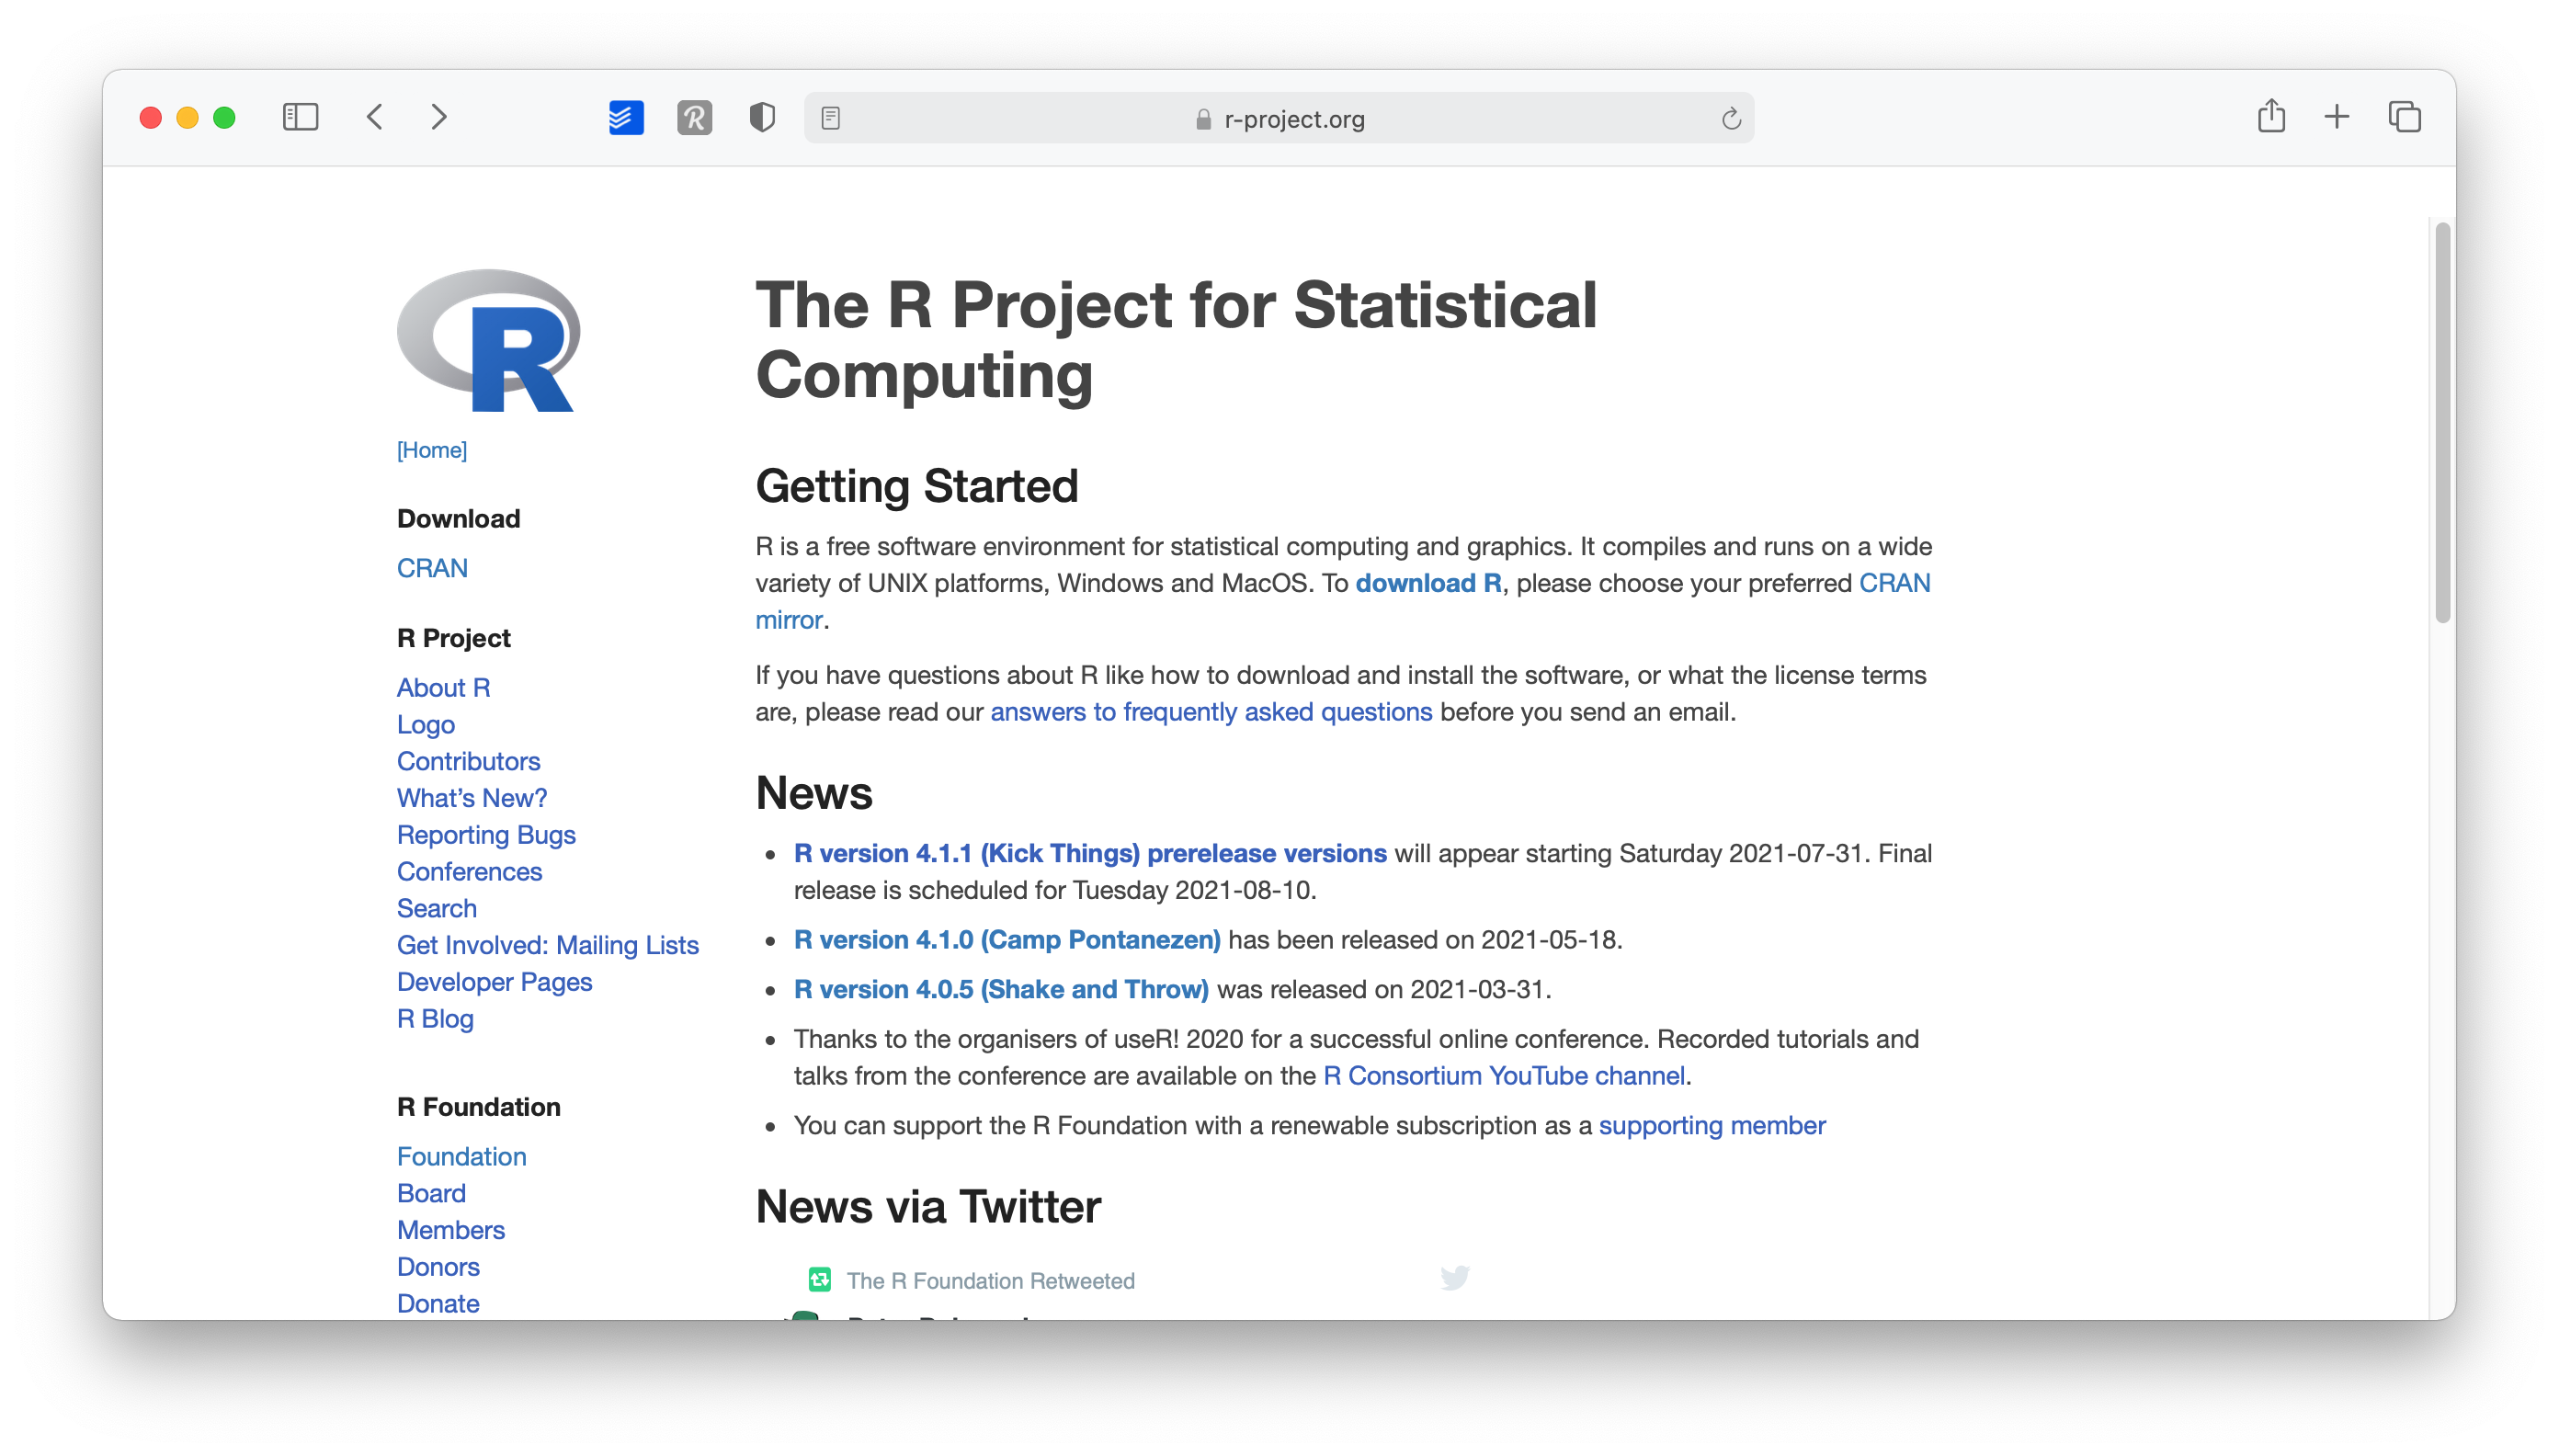
\includegraphics{images/chapter_03_img/r_project/00_r_project_page.png}
\item
  Click on \texttt{CRAN} where it says \texttt{Download}.
\item
  Choose a server in your country (all of them work, but downloads will
  perform quicker if you choose your country or one that is close to
  where you are).

  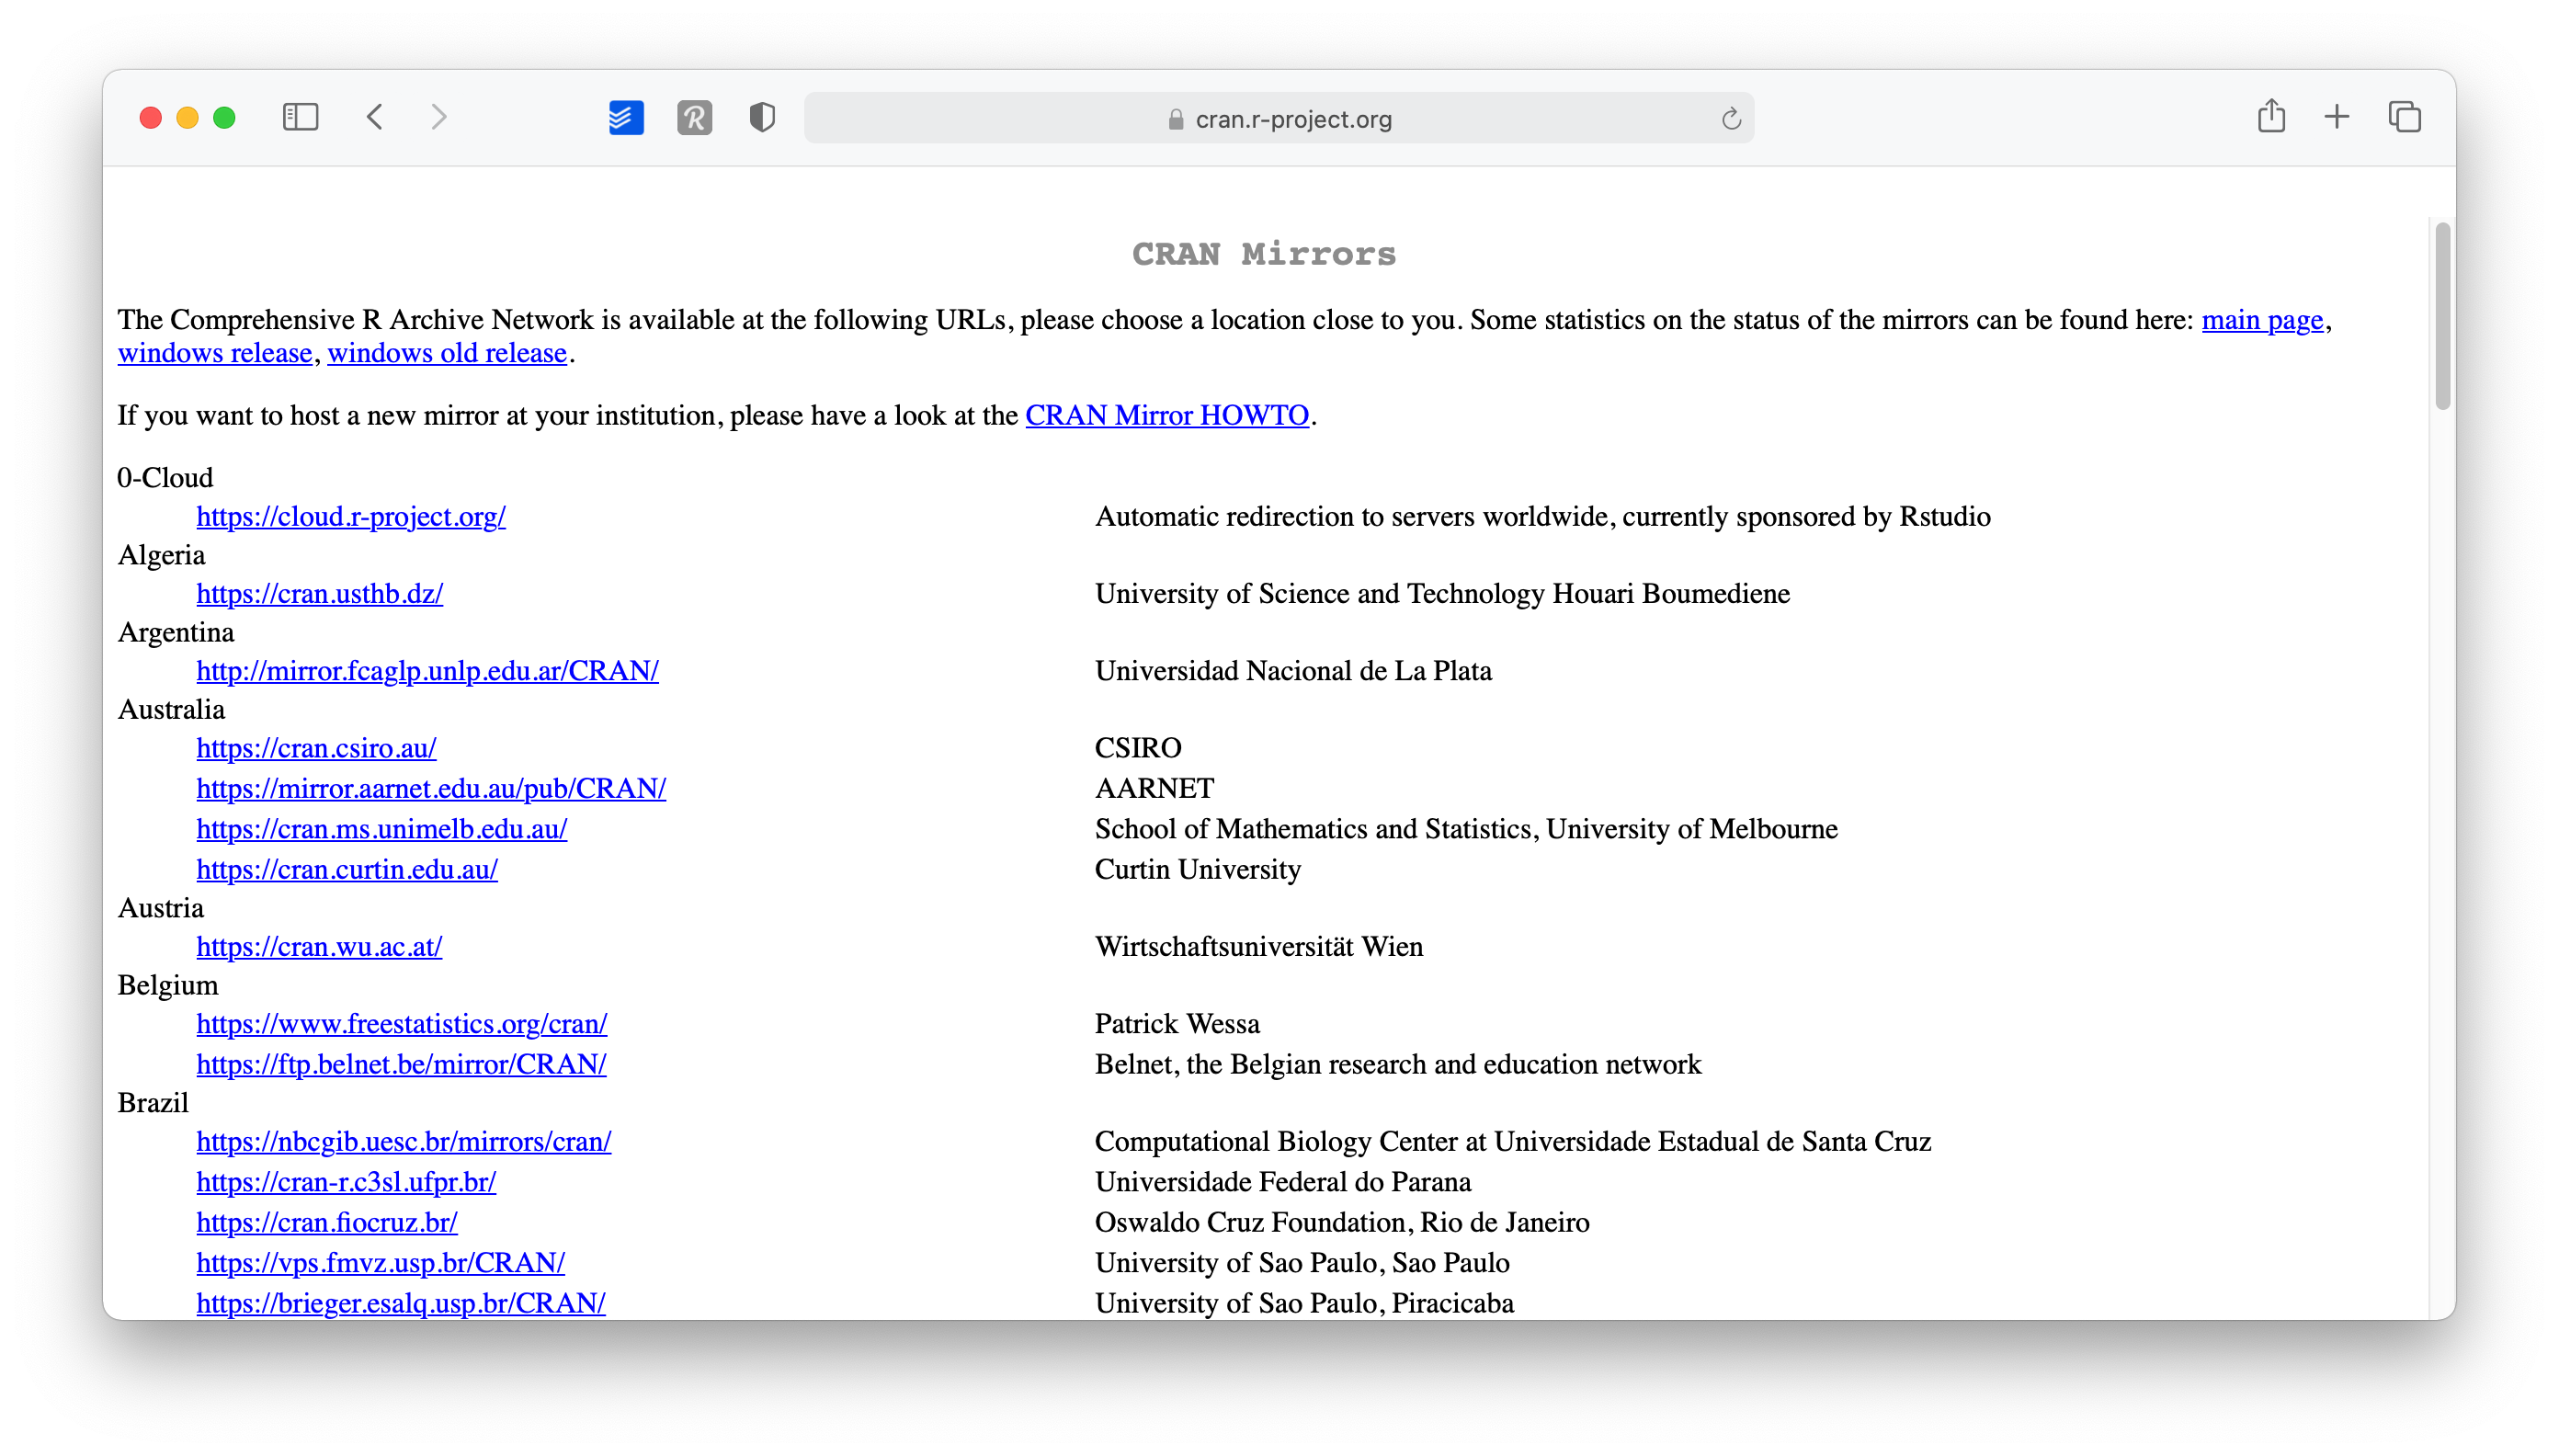
\includegraphics{images/chapter_03_img/r_project/01_r_project_cran_mirror.png}
\item
  Select the operating system for your computer, for example
  \texttt{Download\ R\ for\ macOS}.

  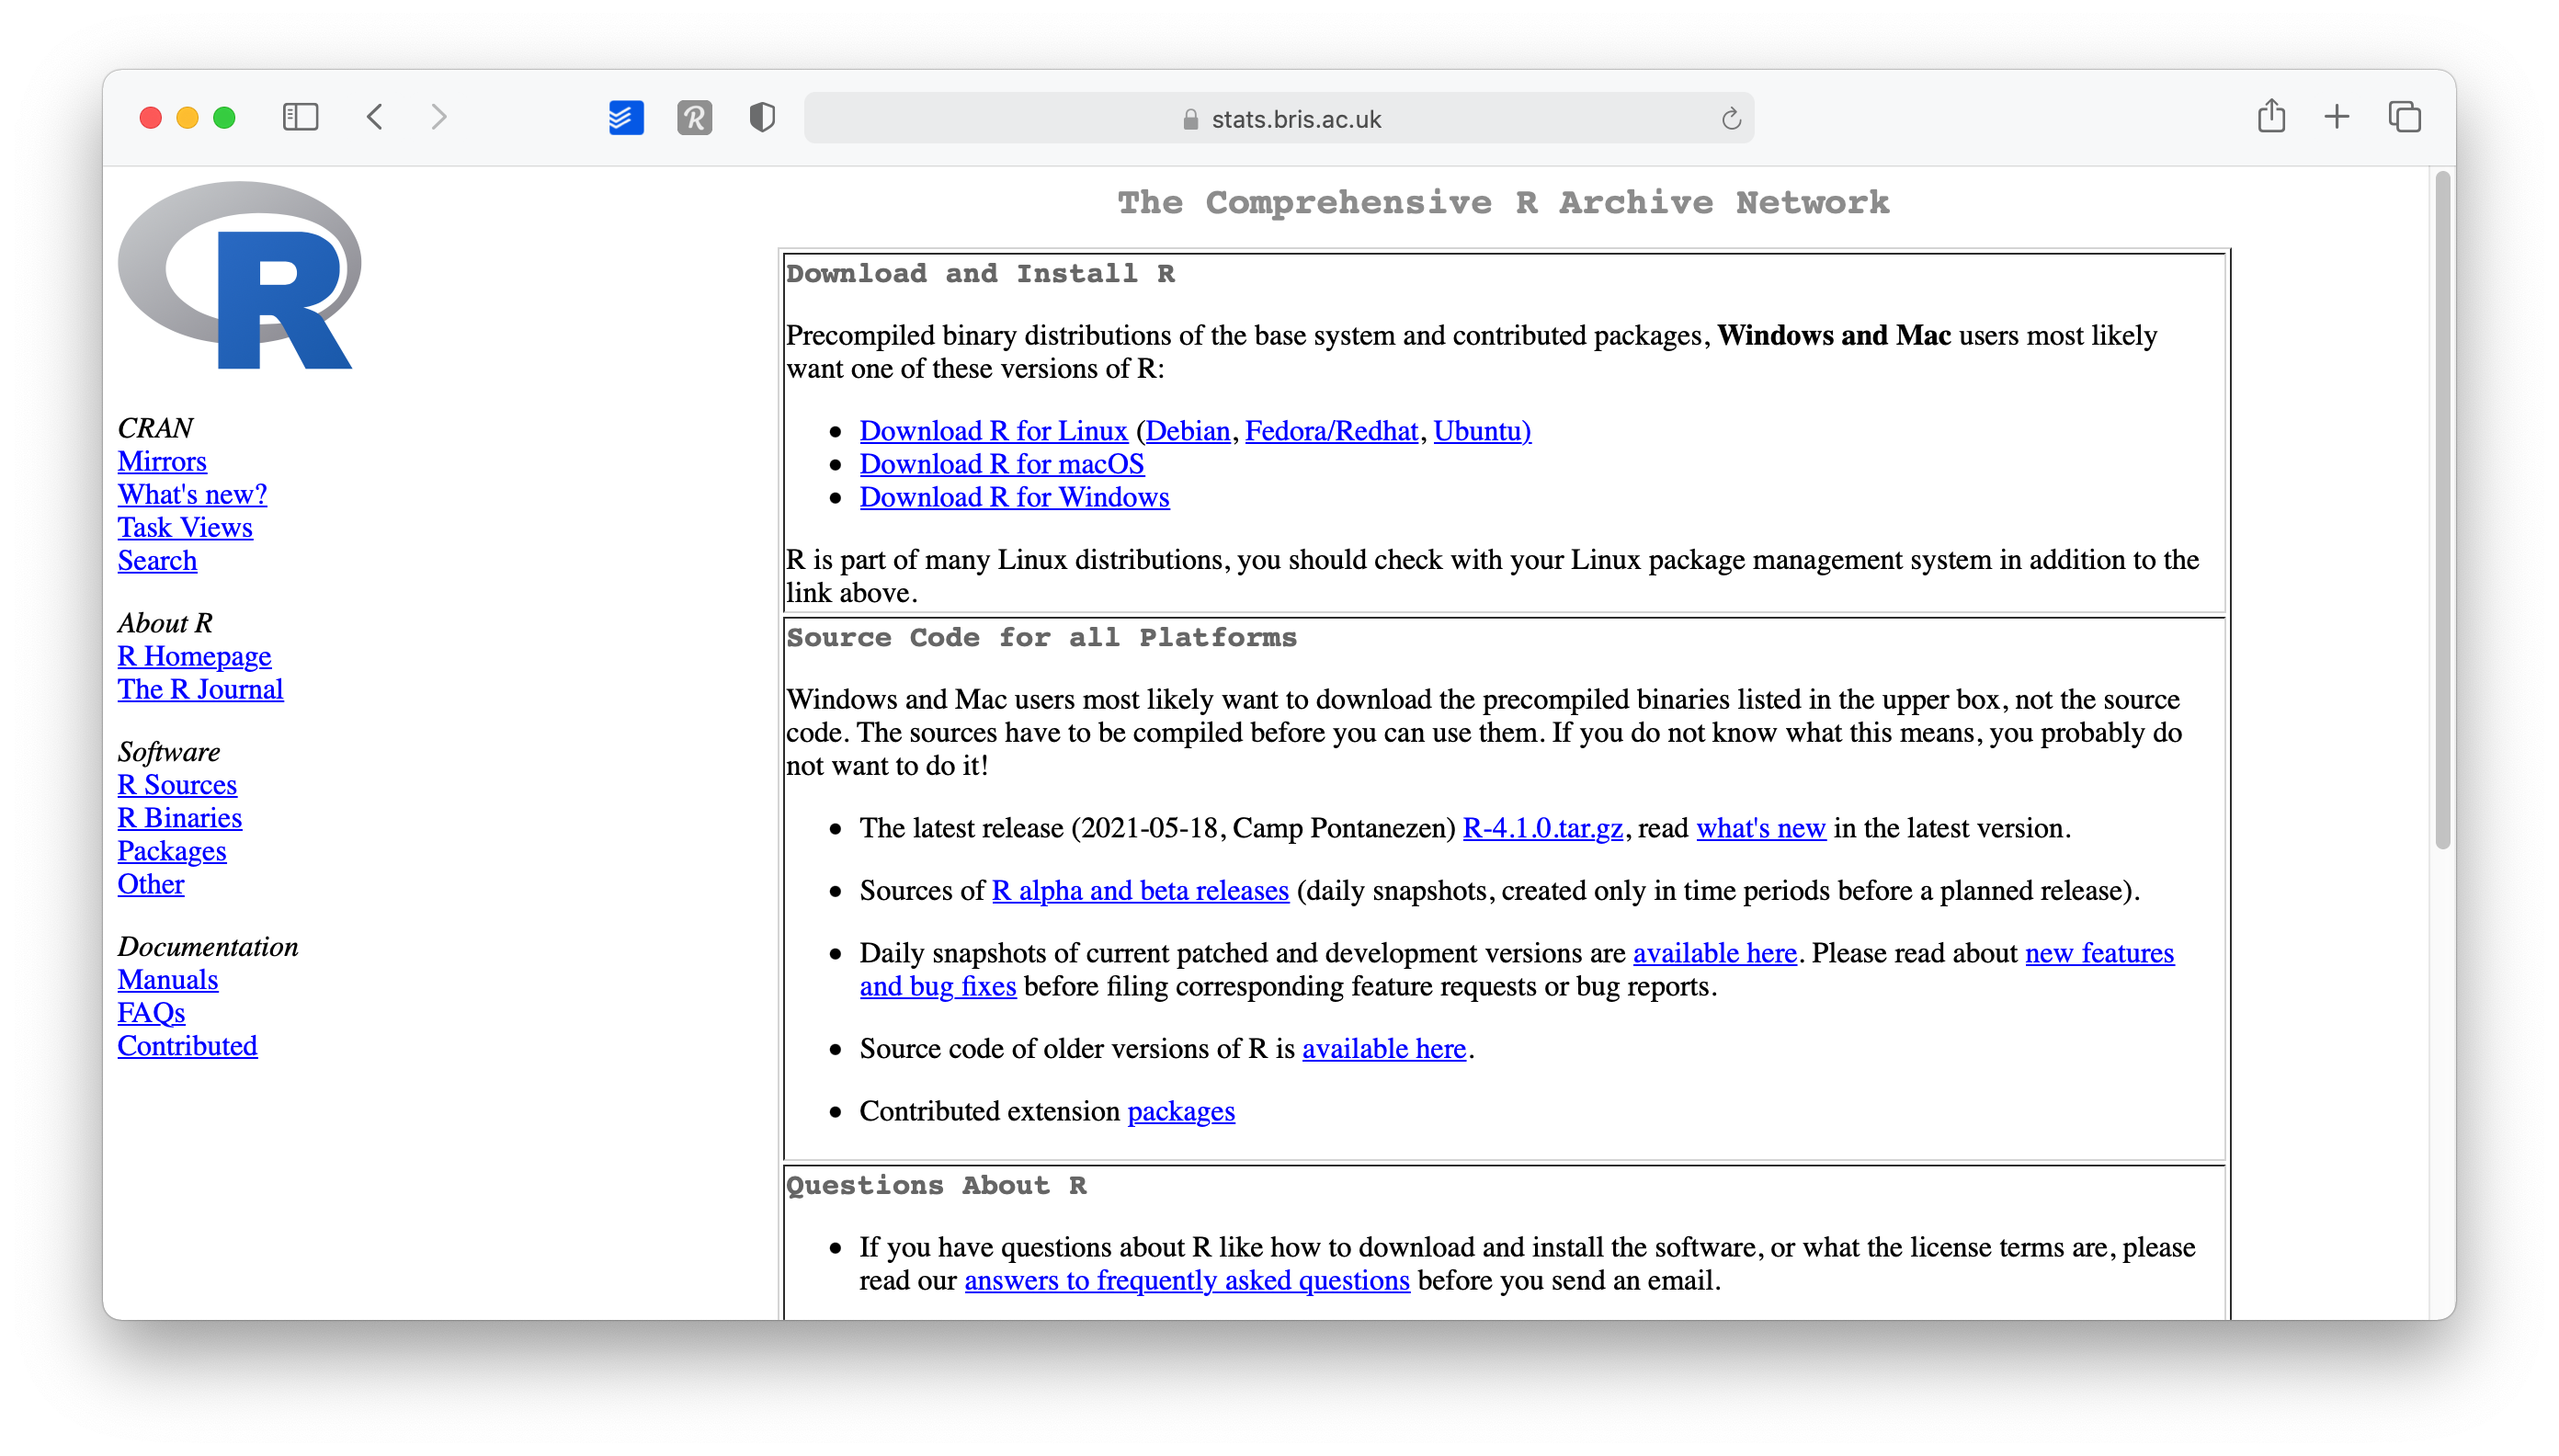
\includegraphics{images/chapter_03_img/r_project/02_r_project_os_choice.png}
\item
  Select the version you want to install (I recommend the latest
  version)

  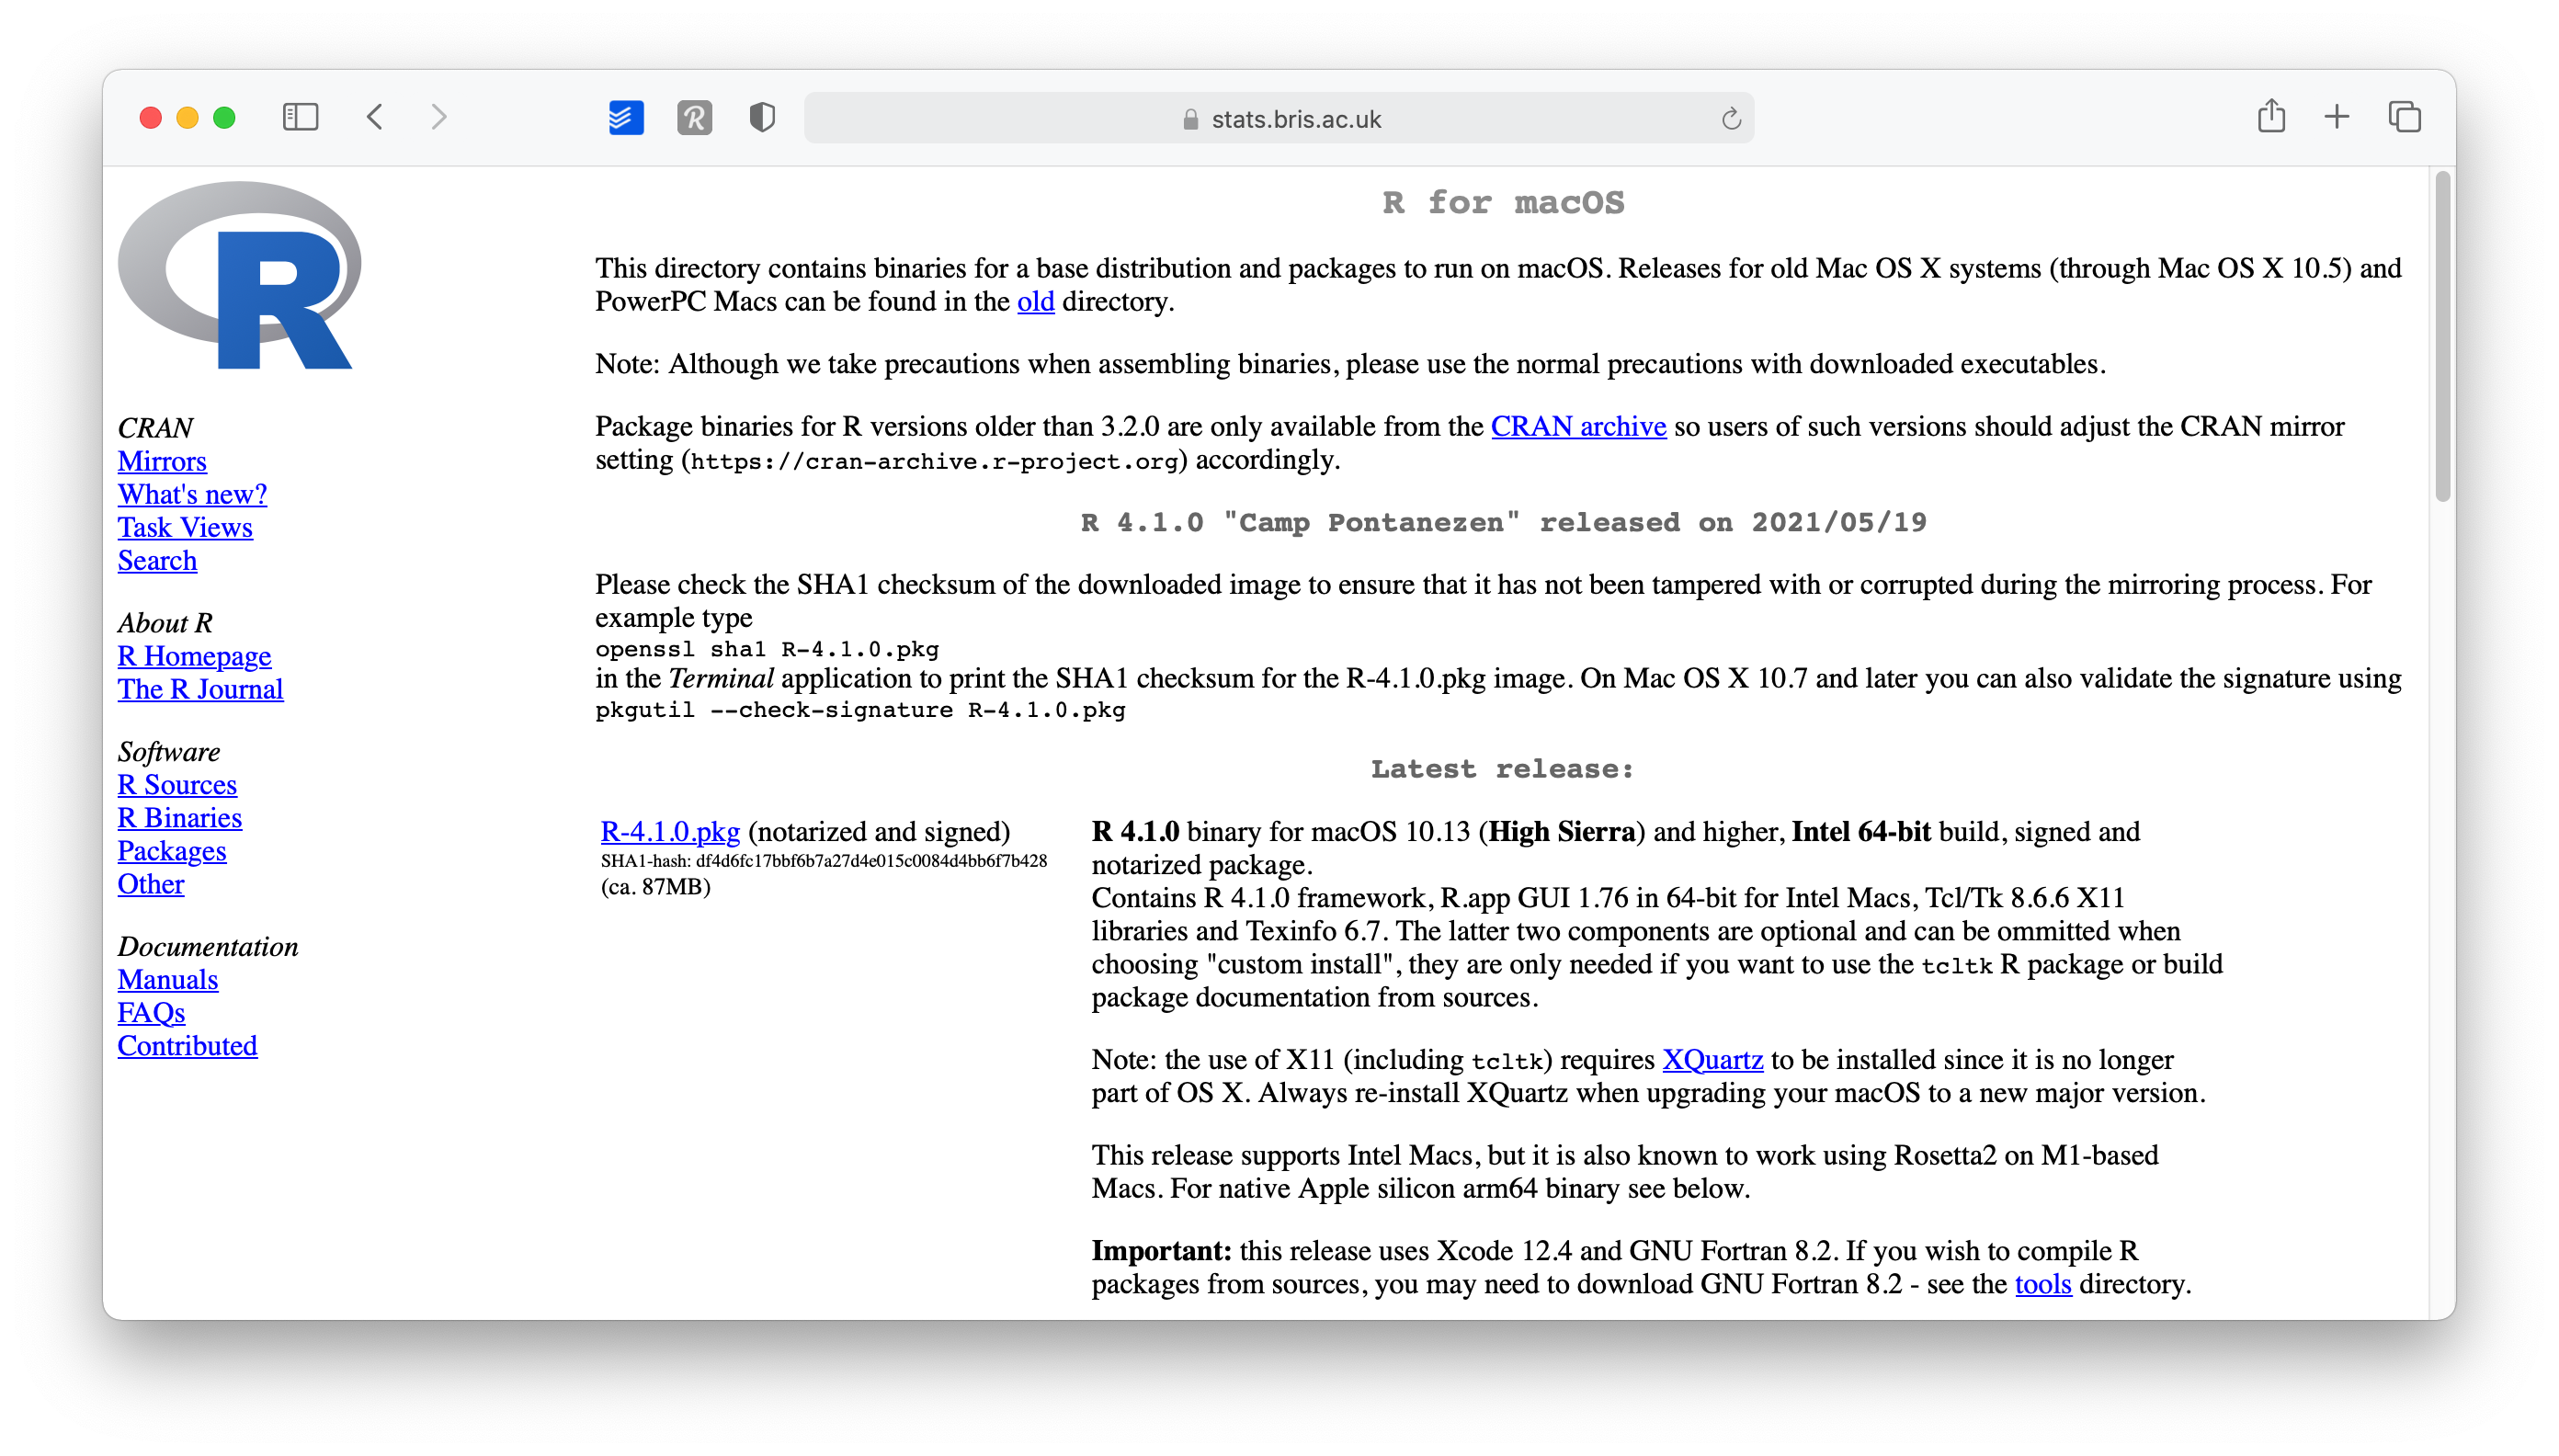
\includegraphics{images/chapter_03_img/r_project/03_r_project_version_choice.png}
\item
  Open the downloaded file and follow the installation instructions. I
  recommend leaving the suggested settings as they are.
\end{enumerate}

This was relatively easy. You now have \emph{R} installed. Technically,
you can start using \emph{R} for your research, but there is one more
tool I strongly advise installing: RStudio.

\section{Installing RStudio}\label{sec-installing-rstudio}

\emph{R} by itself is just the `beating heart' of \emph{R} programming,
but it has no particular user interface. If you want buttons to click
and actually `see' what you are doing, there is no better way than
RStudio. RStudio is an \emph{integrated development environment} (IDE)
and will be our primary tool to interact with \emph{R}. It is the only
software you need to do all the fun parts and, of course, to follow
along with the examples in this book. To install RStudio, perform the
following steps:

\begin{enumerate}
\def\labelenumi{\arabic{enumi}.}
\item
  Go to \url{http://posit.co} and click on \texttt{DOWNLOAD\ RSTUDIO}.

  
\includegraphics{images/chapter_03_img/rstudio/01_posit_main_page.png}
\item
  Click on \texttt{DOWNLOAD\ RSTUDIO} on this page.

  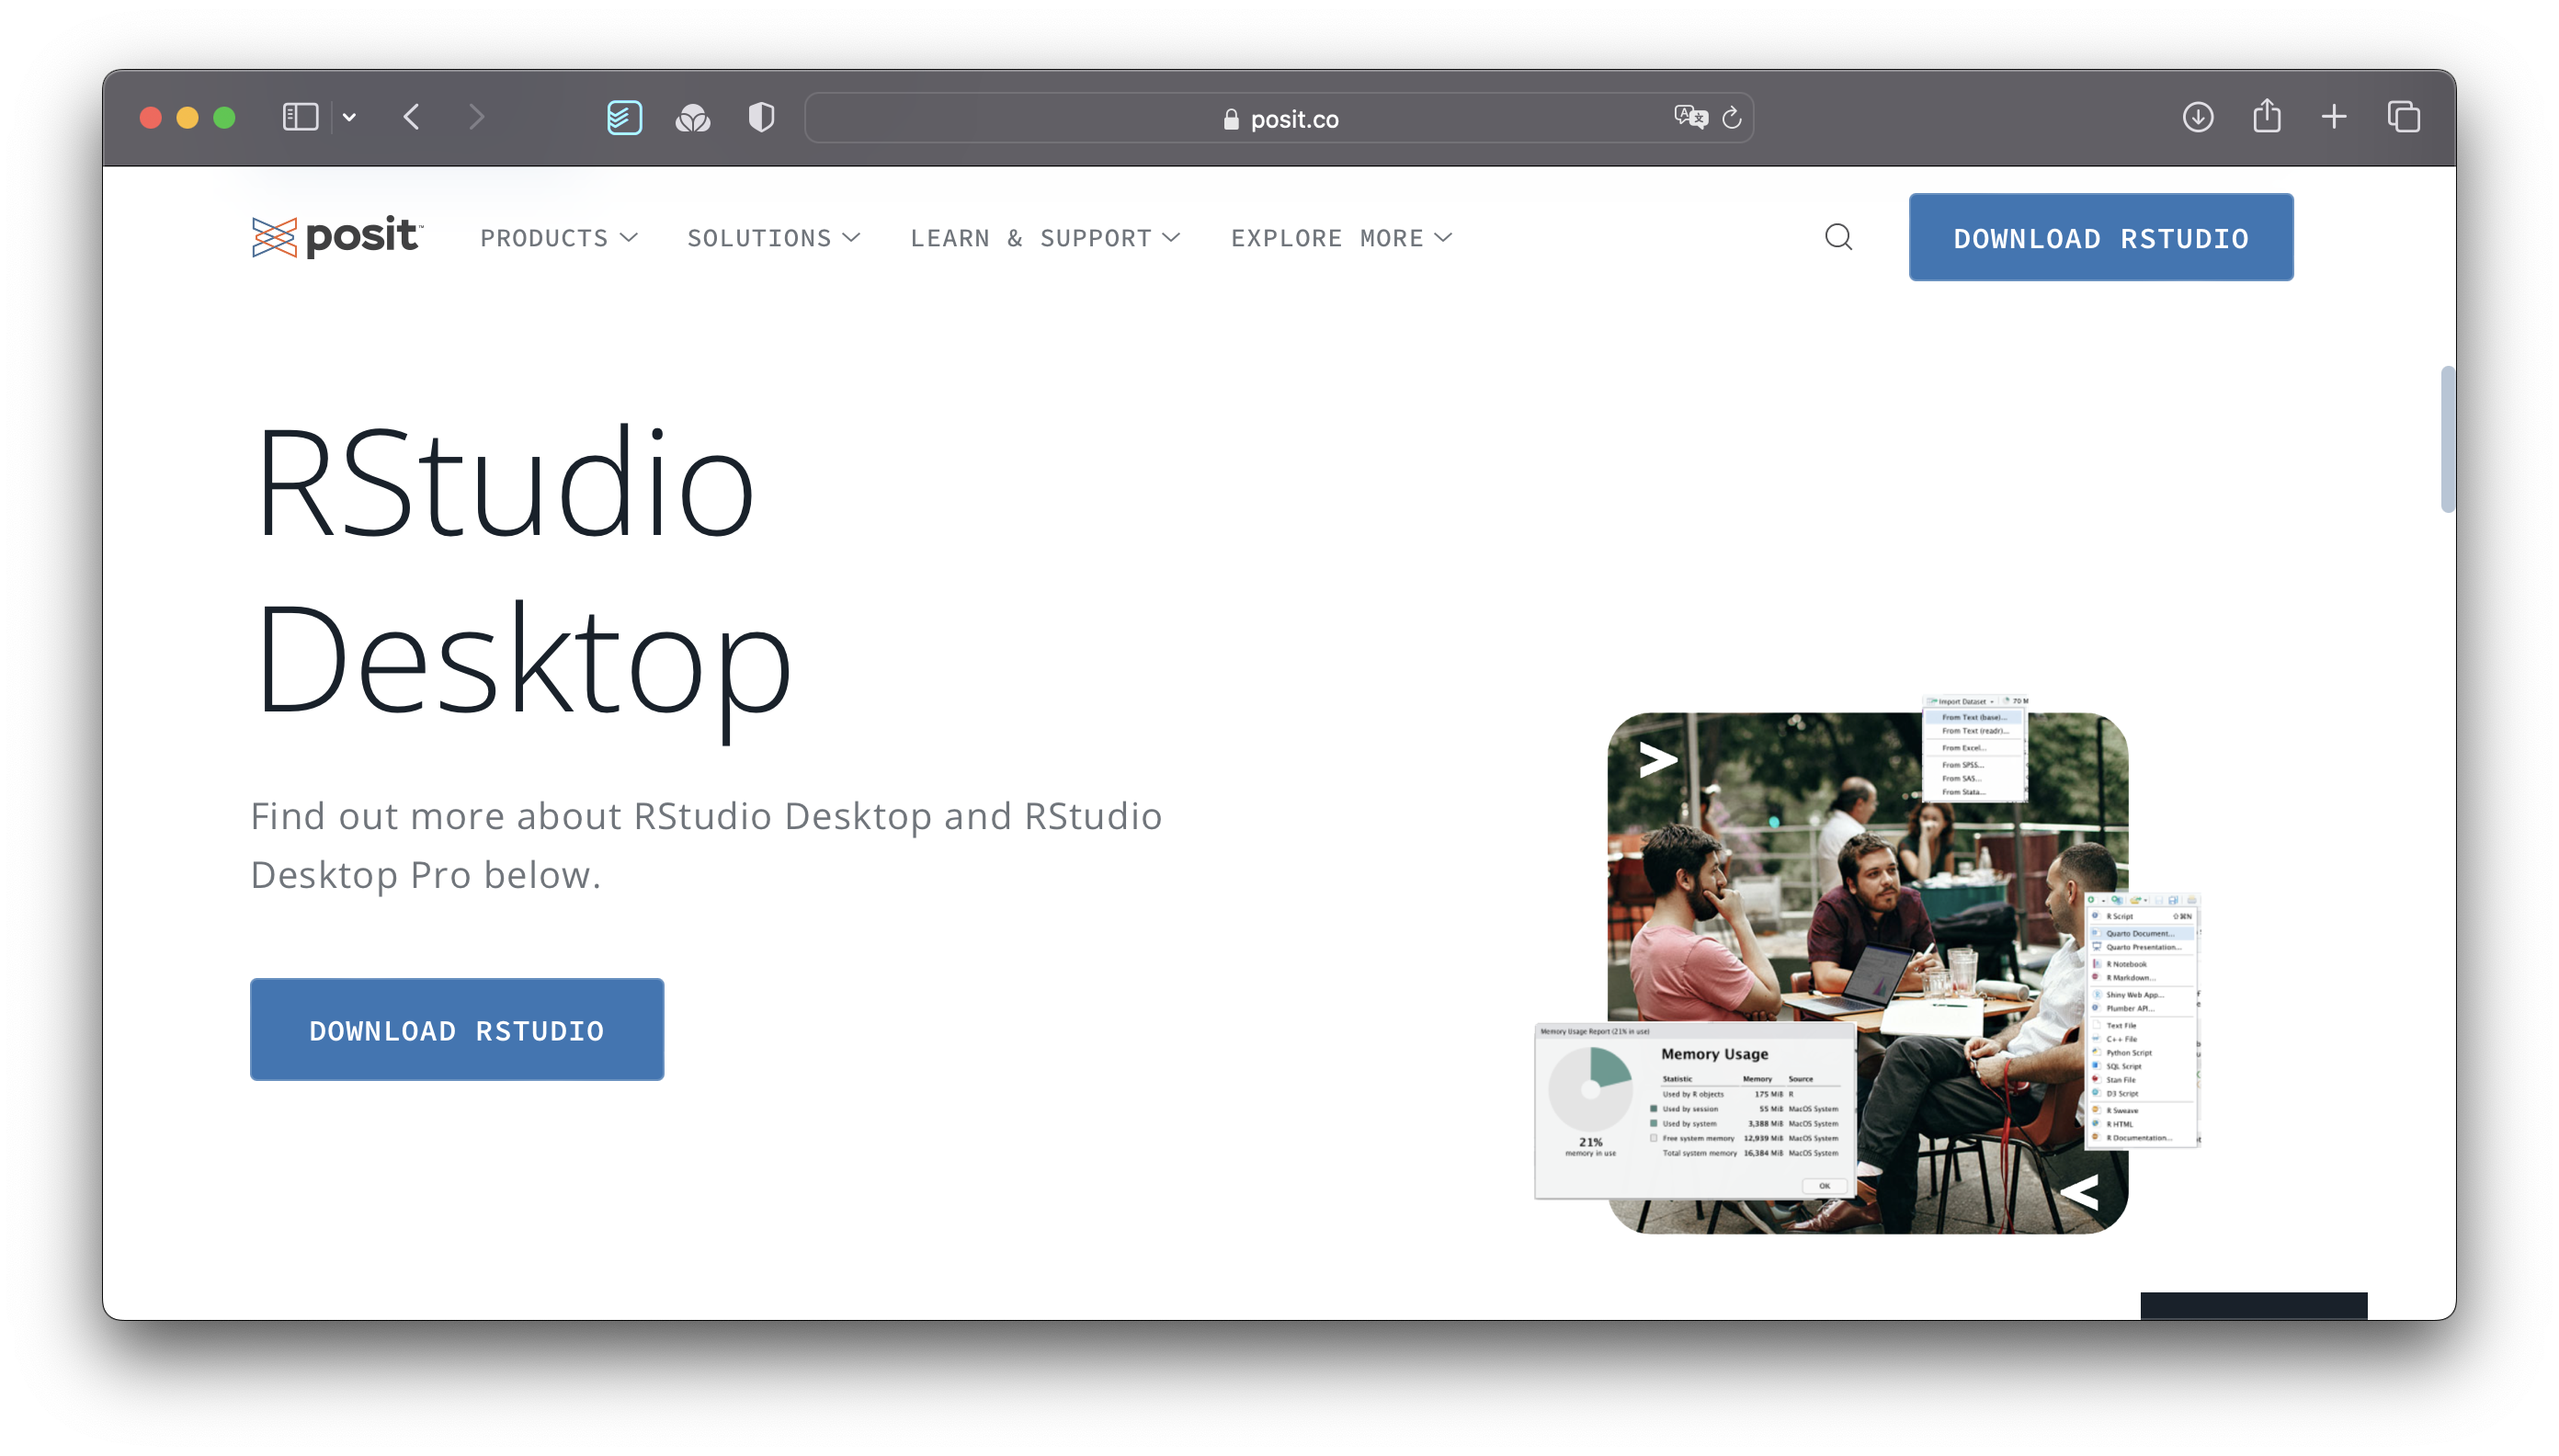
\includegraphics{images/chapter_03_img/rstudio/02_posit_rstudio_desktop.png}
\item
  This leads you to the page where you can install \emph{R} as a first
  step and RStudio as a second step. Since we installed \emph{R}
  already, we can click on
  \texttt{DOWNLOAD\ RSTUDIO\ DESKTOP\ FOR\ WINDOWS} (or for Mac if you
  are not using a PC).

  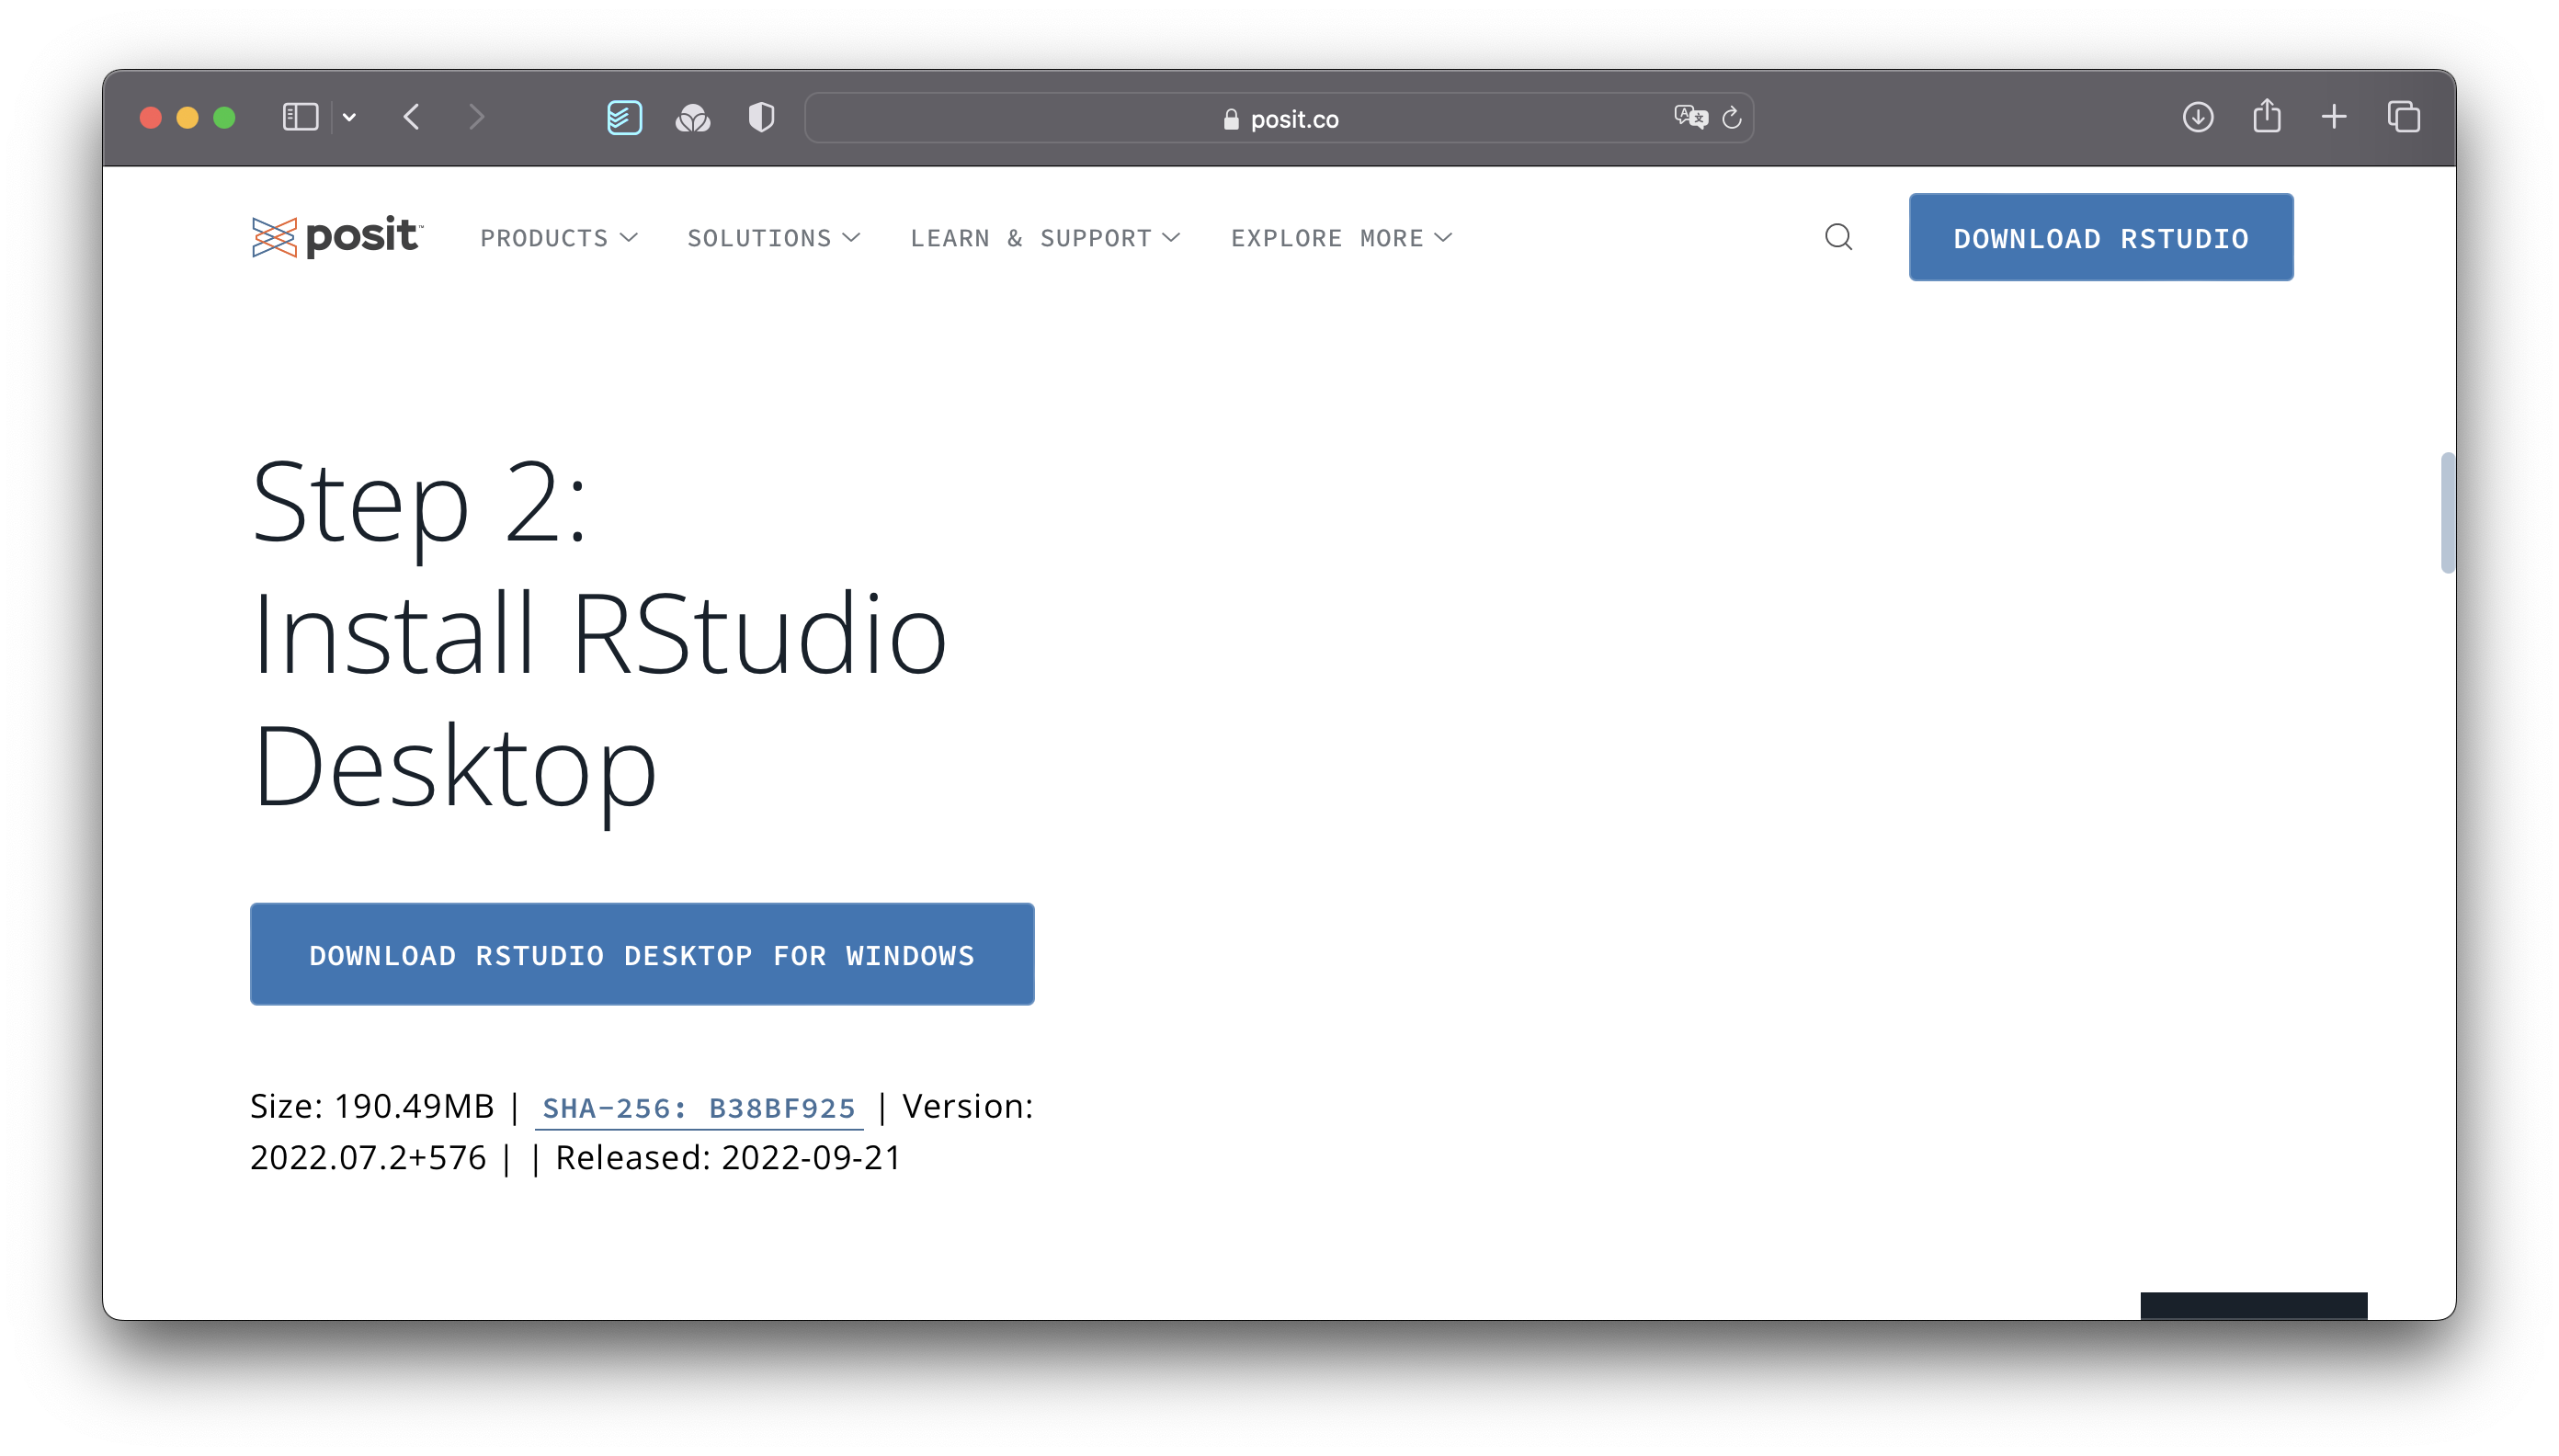
\includegraphics{images/chapter_03_img/rstudio/03_posit_installer.png}
\item
  If, for some reason, the version for your operating system is not
  showing up correctly, you can scroll down and find other versions
  ready to be installed.

  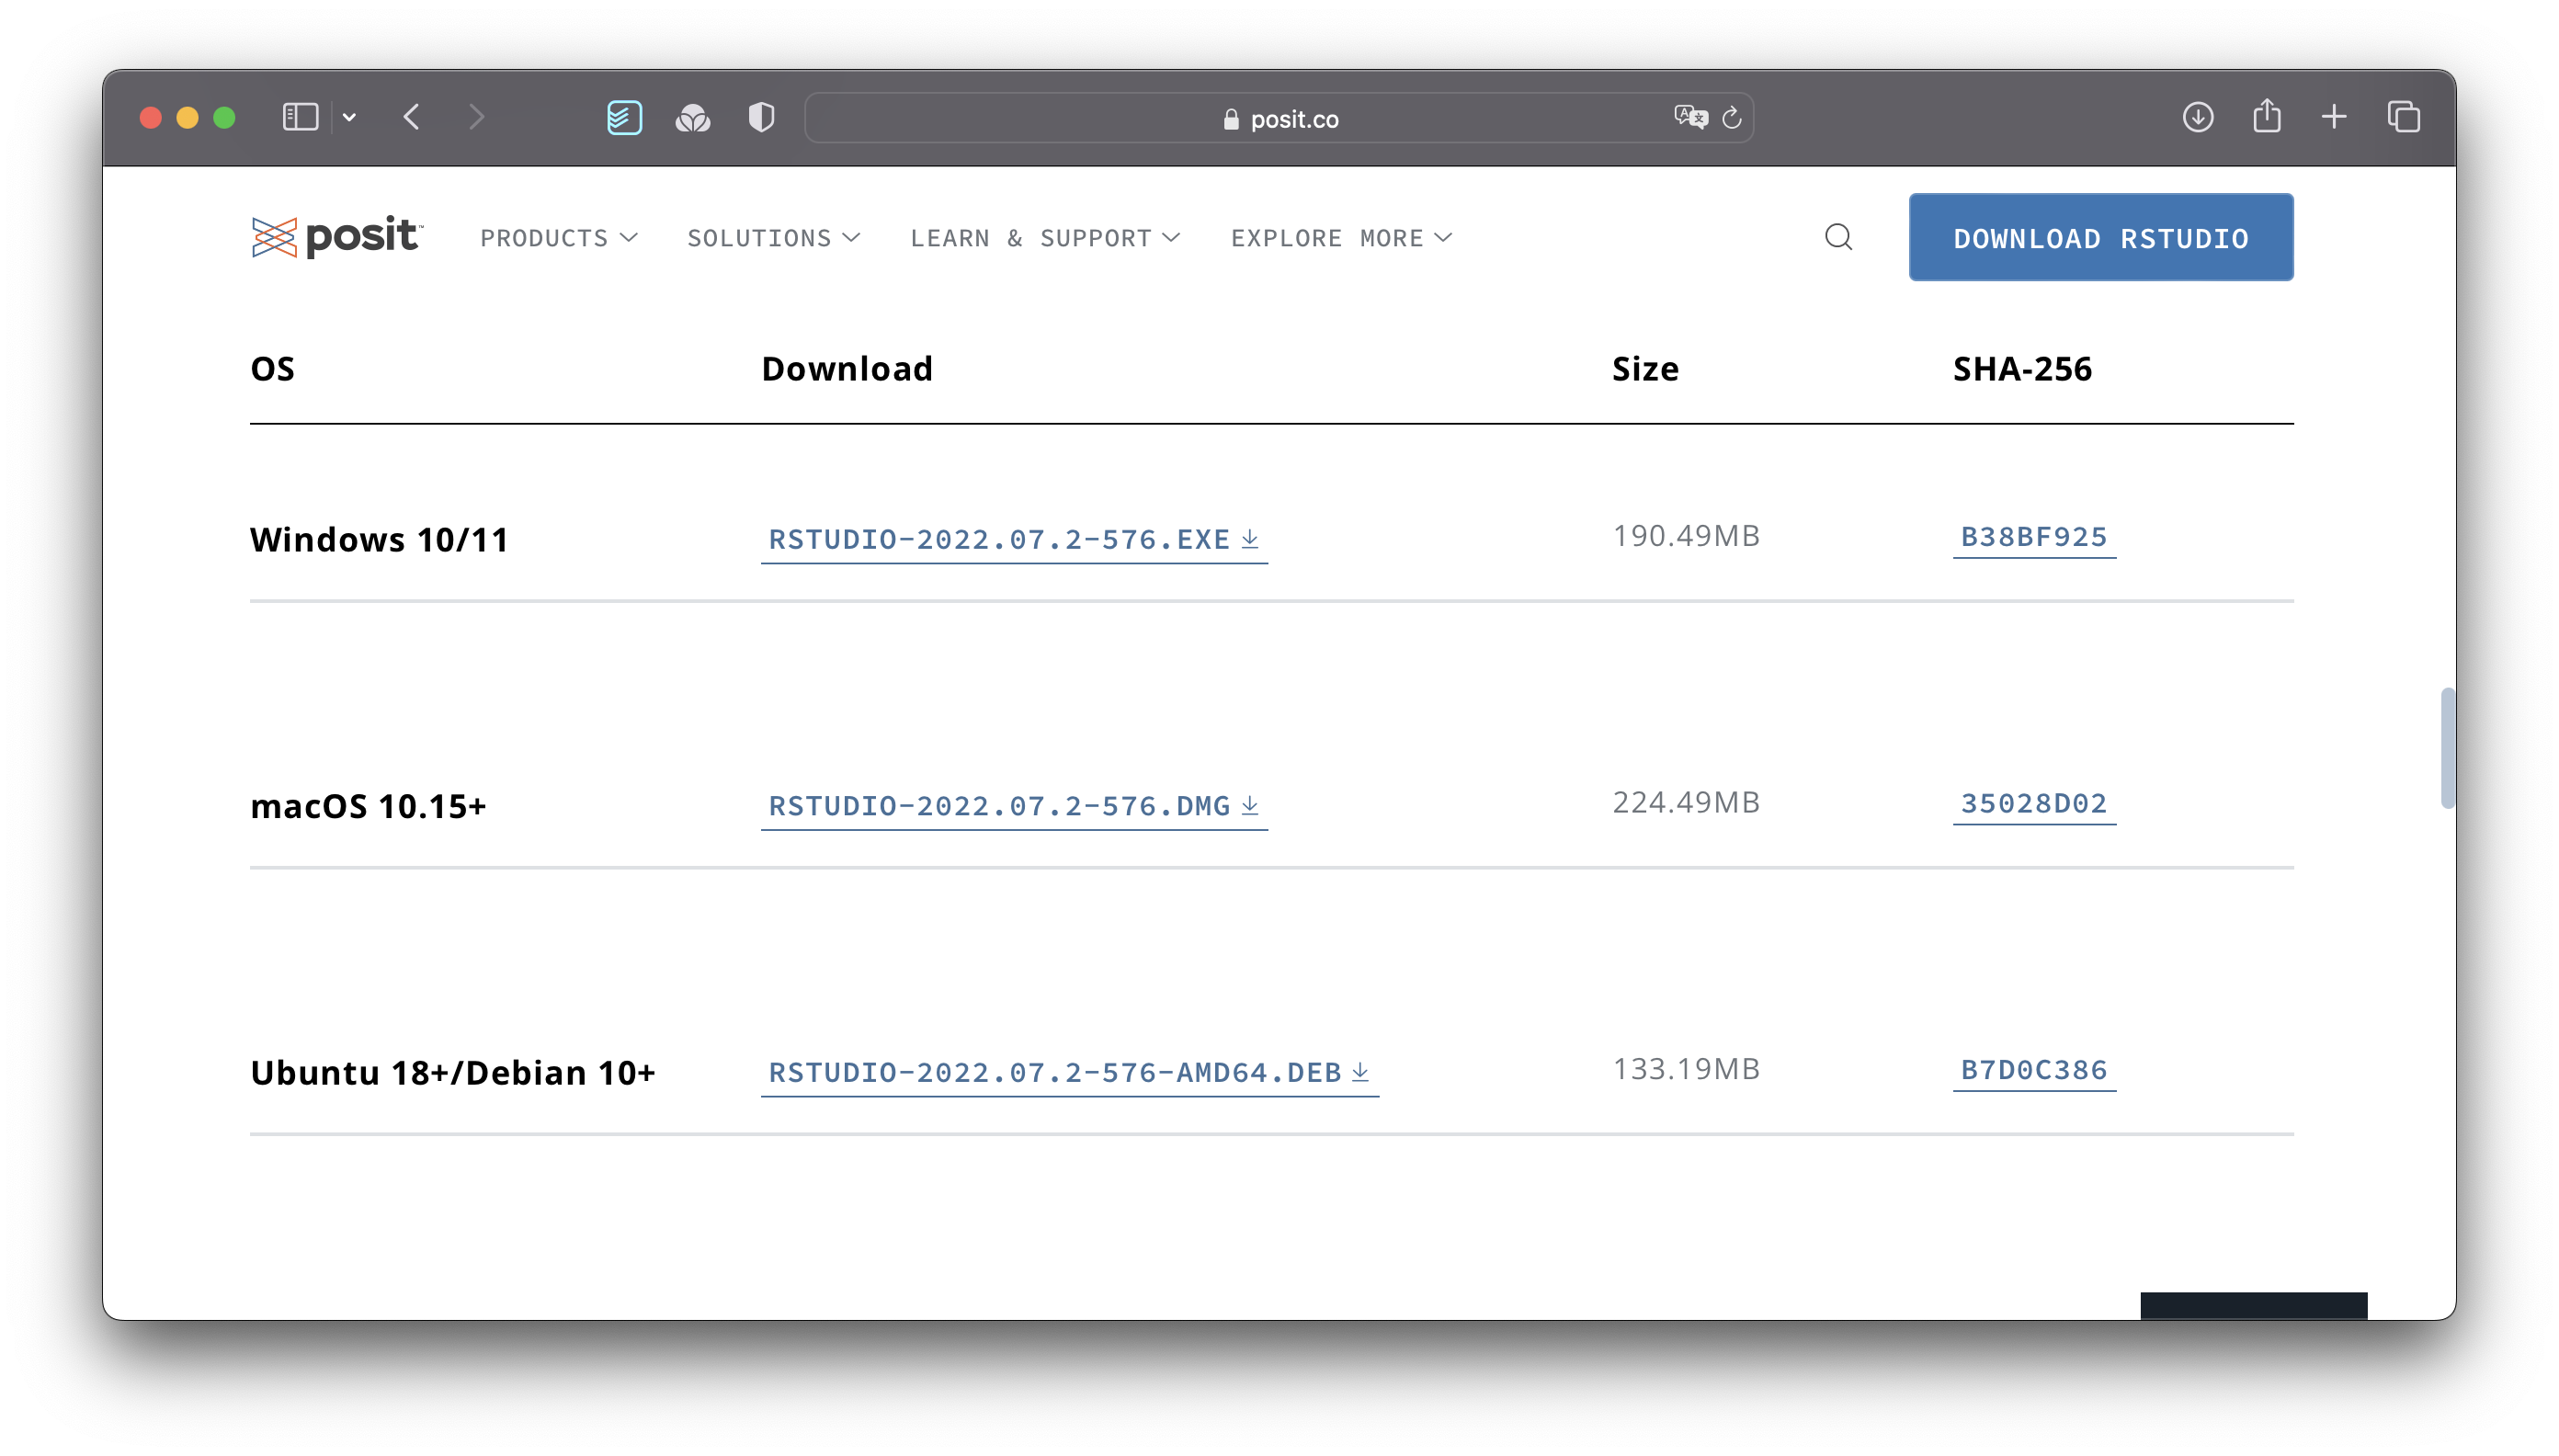
\includegraphics{images/chapter_03_img/rstudio/04_other_installers.png}
\item
  Open the downloaded file and follow the installation instructions.
  Again, stick with the default settings as much as possible.
\end{enumerate}

Congratulations, you are all set up to learn \emph{R}. From now on, you
only need to start RStudio and not \emph{R}. Of course, if you are the
curious type, nothing shall stop you from trying \emph{R} without
RStudio.

\section{When you first start
RStudio}\label{sec-when-you-first-start-rstudio}

Before you start programming away, you might want to tweak some of your
settings right away to have a better experience (in my humble opinion).
To open the Rstudio settings, you have to click on

\begin{itemize}
\item
  \texttt{RStudio\ \textgreater{}\ Tools\ \textgreater{}\ Global\ Options}
  or press \texttt{⌘\ +\ ,} if you are on a Mac.
\item
  \texttt{RStudio\ \textgreater{}\ Tools\ \textgreater{}\ Global\ Options}
  or press \texttt{Ctrl\ +\ ,} if you are working on a Windows computer.
\end{itemize}

I recommend to at least make the following changes to set yourself up
for success right from the start:

\begin{enumerate}
\def\labelenumi{\arabic{enumi}.}
\item
  Already on the first tab,
  i.e.~\texttt{General\ \textgreater{}\ Basic}, we should make one of
  the most significant changes. Deactivate every option that starts with
  \texttt{Restore}. This will ensure that every time you start RStudio,
  you begin with a clean slate. At first sight, it might sound
  counter-intuitive not to restart everything where you left off, but it
  is essential to make all your projects easily reproducible.
  Furthermore, if you work together with others, not restoring your
  personal settings also ensures that your programming works across
  different computers. Therefore, I recommend having the following
  unticked:

  \begin{itemize}
  \item
    \texttt{Restore\ most\ recently\ opened\ project\ at\ startup},
  \item
    \texttt{Restore\ previsouly\ open\ source\ documents\ at\ startup},
  \item
    \texttt{Restore\ .Rdata\ into\ workspace\ at\ startup}

    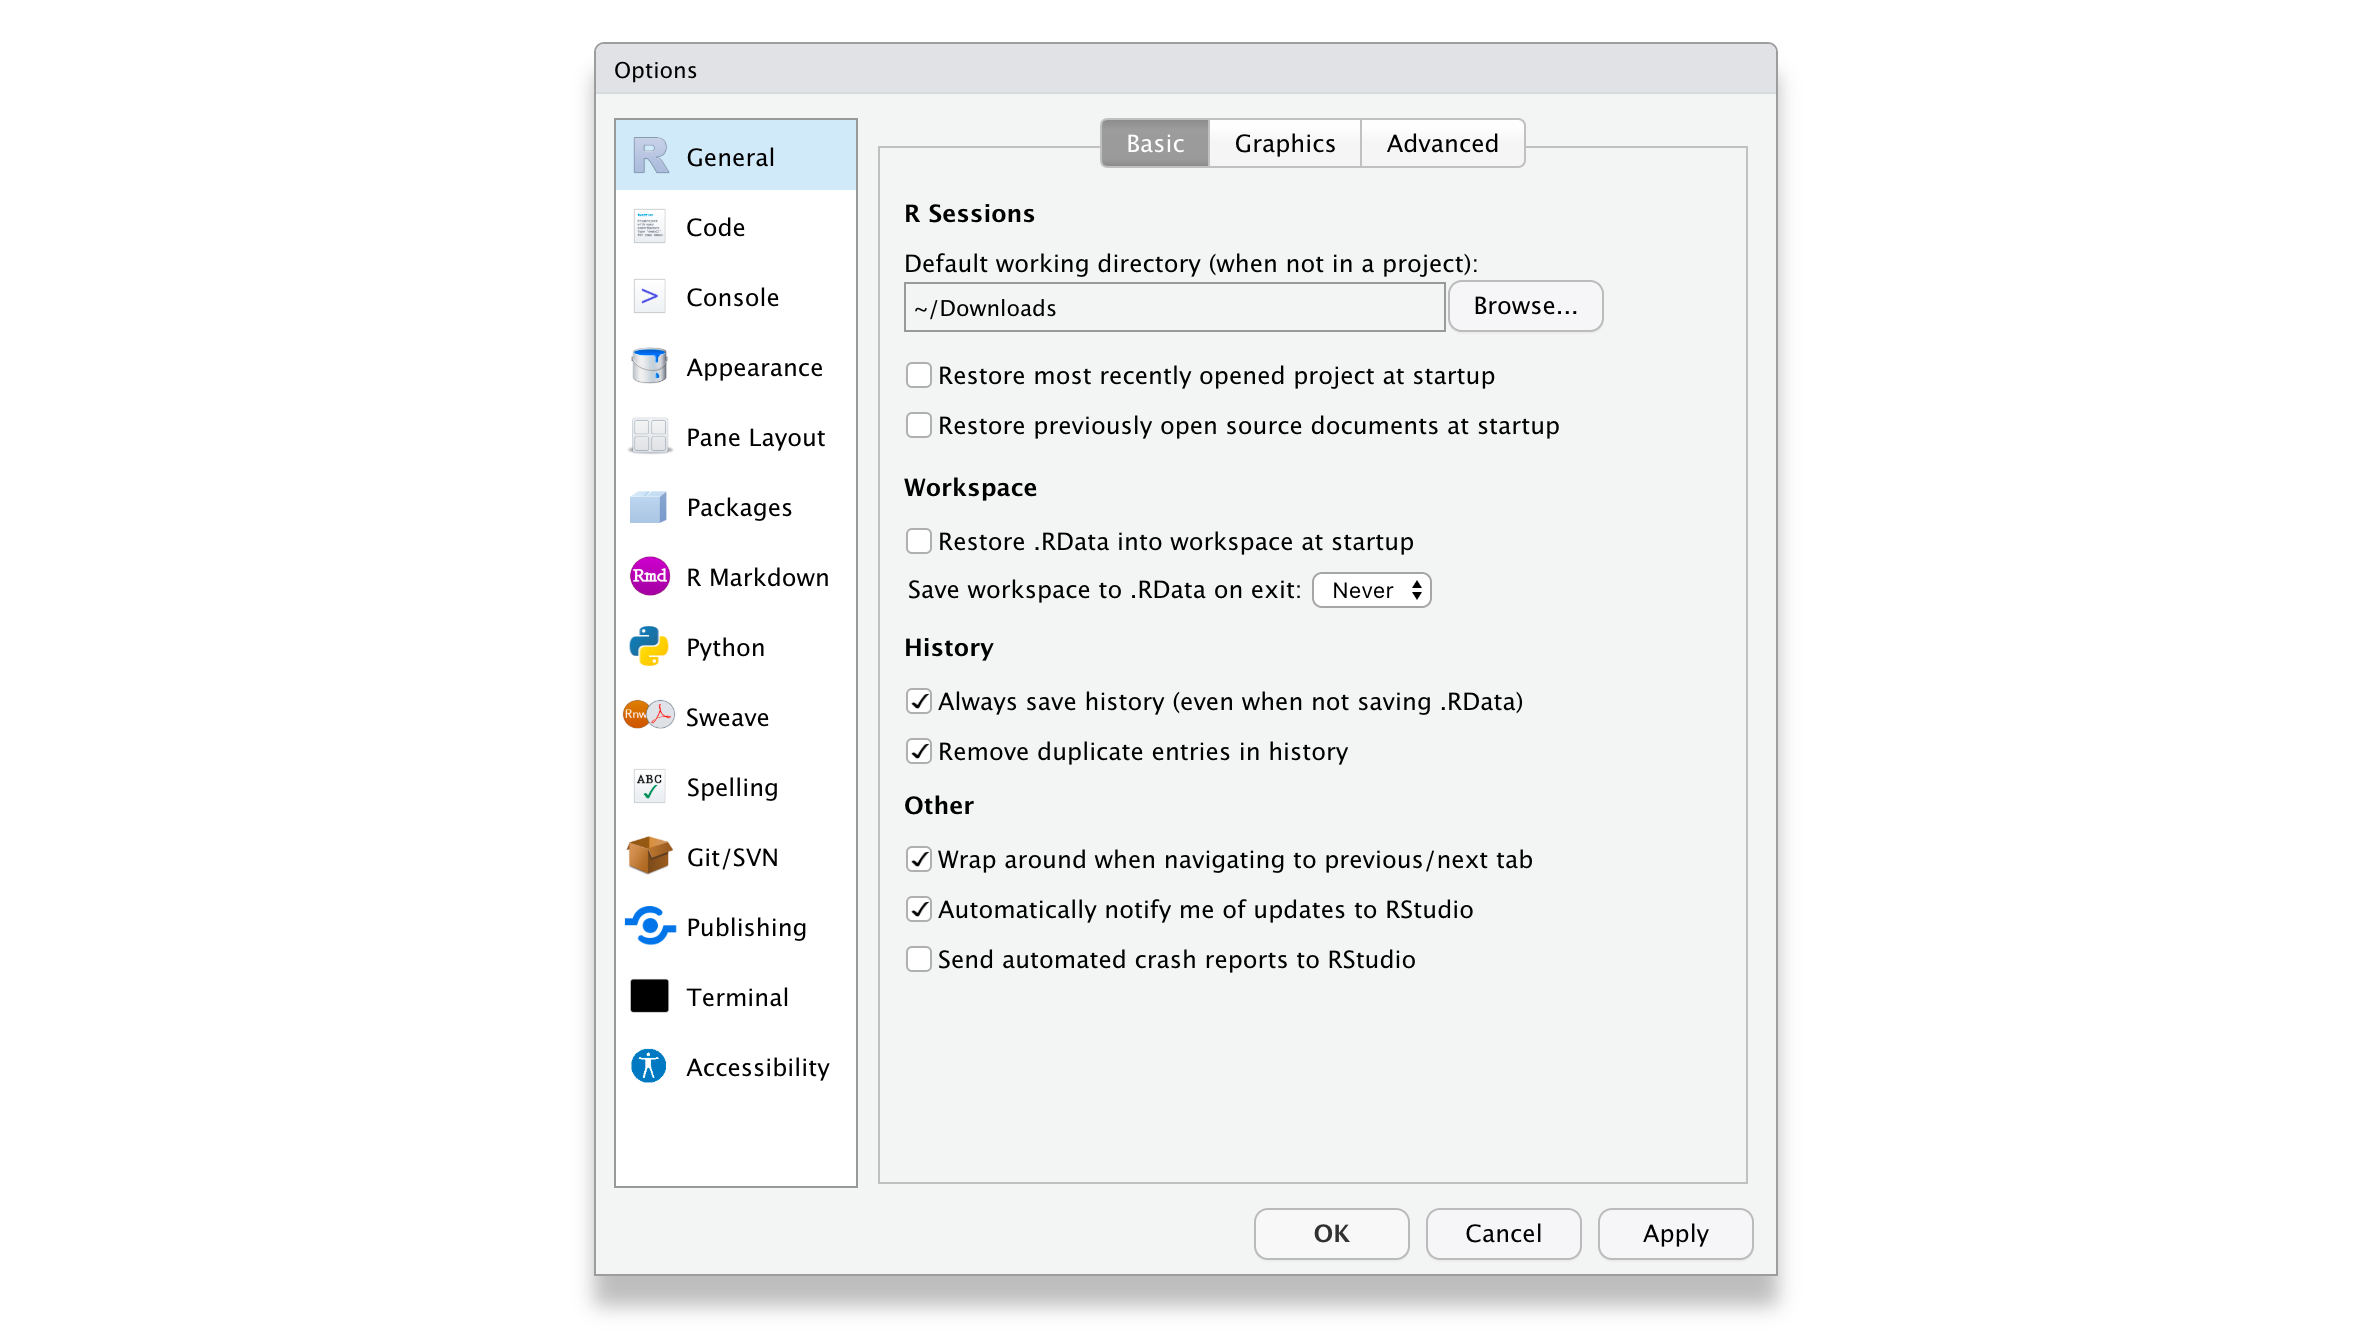
\includegraphics{images/chapter_03_img/rstudio_preferences/00_rstudio_preferences_basic.png}
  \end{itemize}
\item
  In the same tab under \texttt{Workspace}, select \texttt{Never} for
  the setting \texttt{Save\ workspace\ to\ .RData\ on\ exit}. One might
  think it is wise to keep intermediary results stored from one \emph{R}
  session to another. However, I often found myself fixing issues due to
  this lazy method, and my code became less reliable and, therefore,
  less reproducible. With experience, you will find that this avoids
  many headaches.
\item
  In the \texttt{Code\ \textgreater{}\ Editing} tab, make sure to have
  at least the first five options ticked, especially the
  \texttt{Auto-indent\ code\ after\ paste}. This setting will save time
  when formatting your coding appropriately, making it easier to read.
  Indentation is the primary way of making your code look more readable
  and less like a series of characters that appear almost random.

  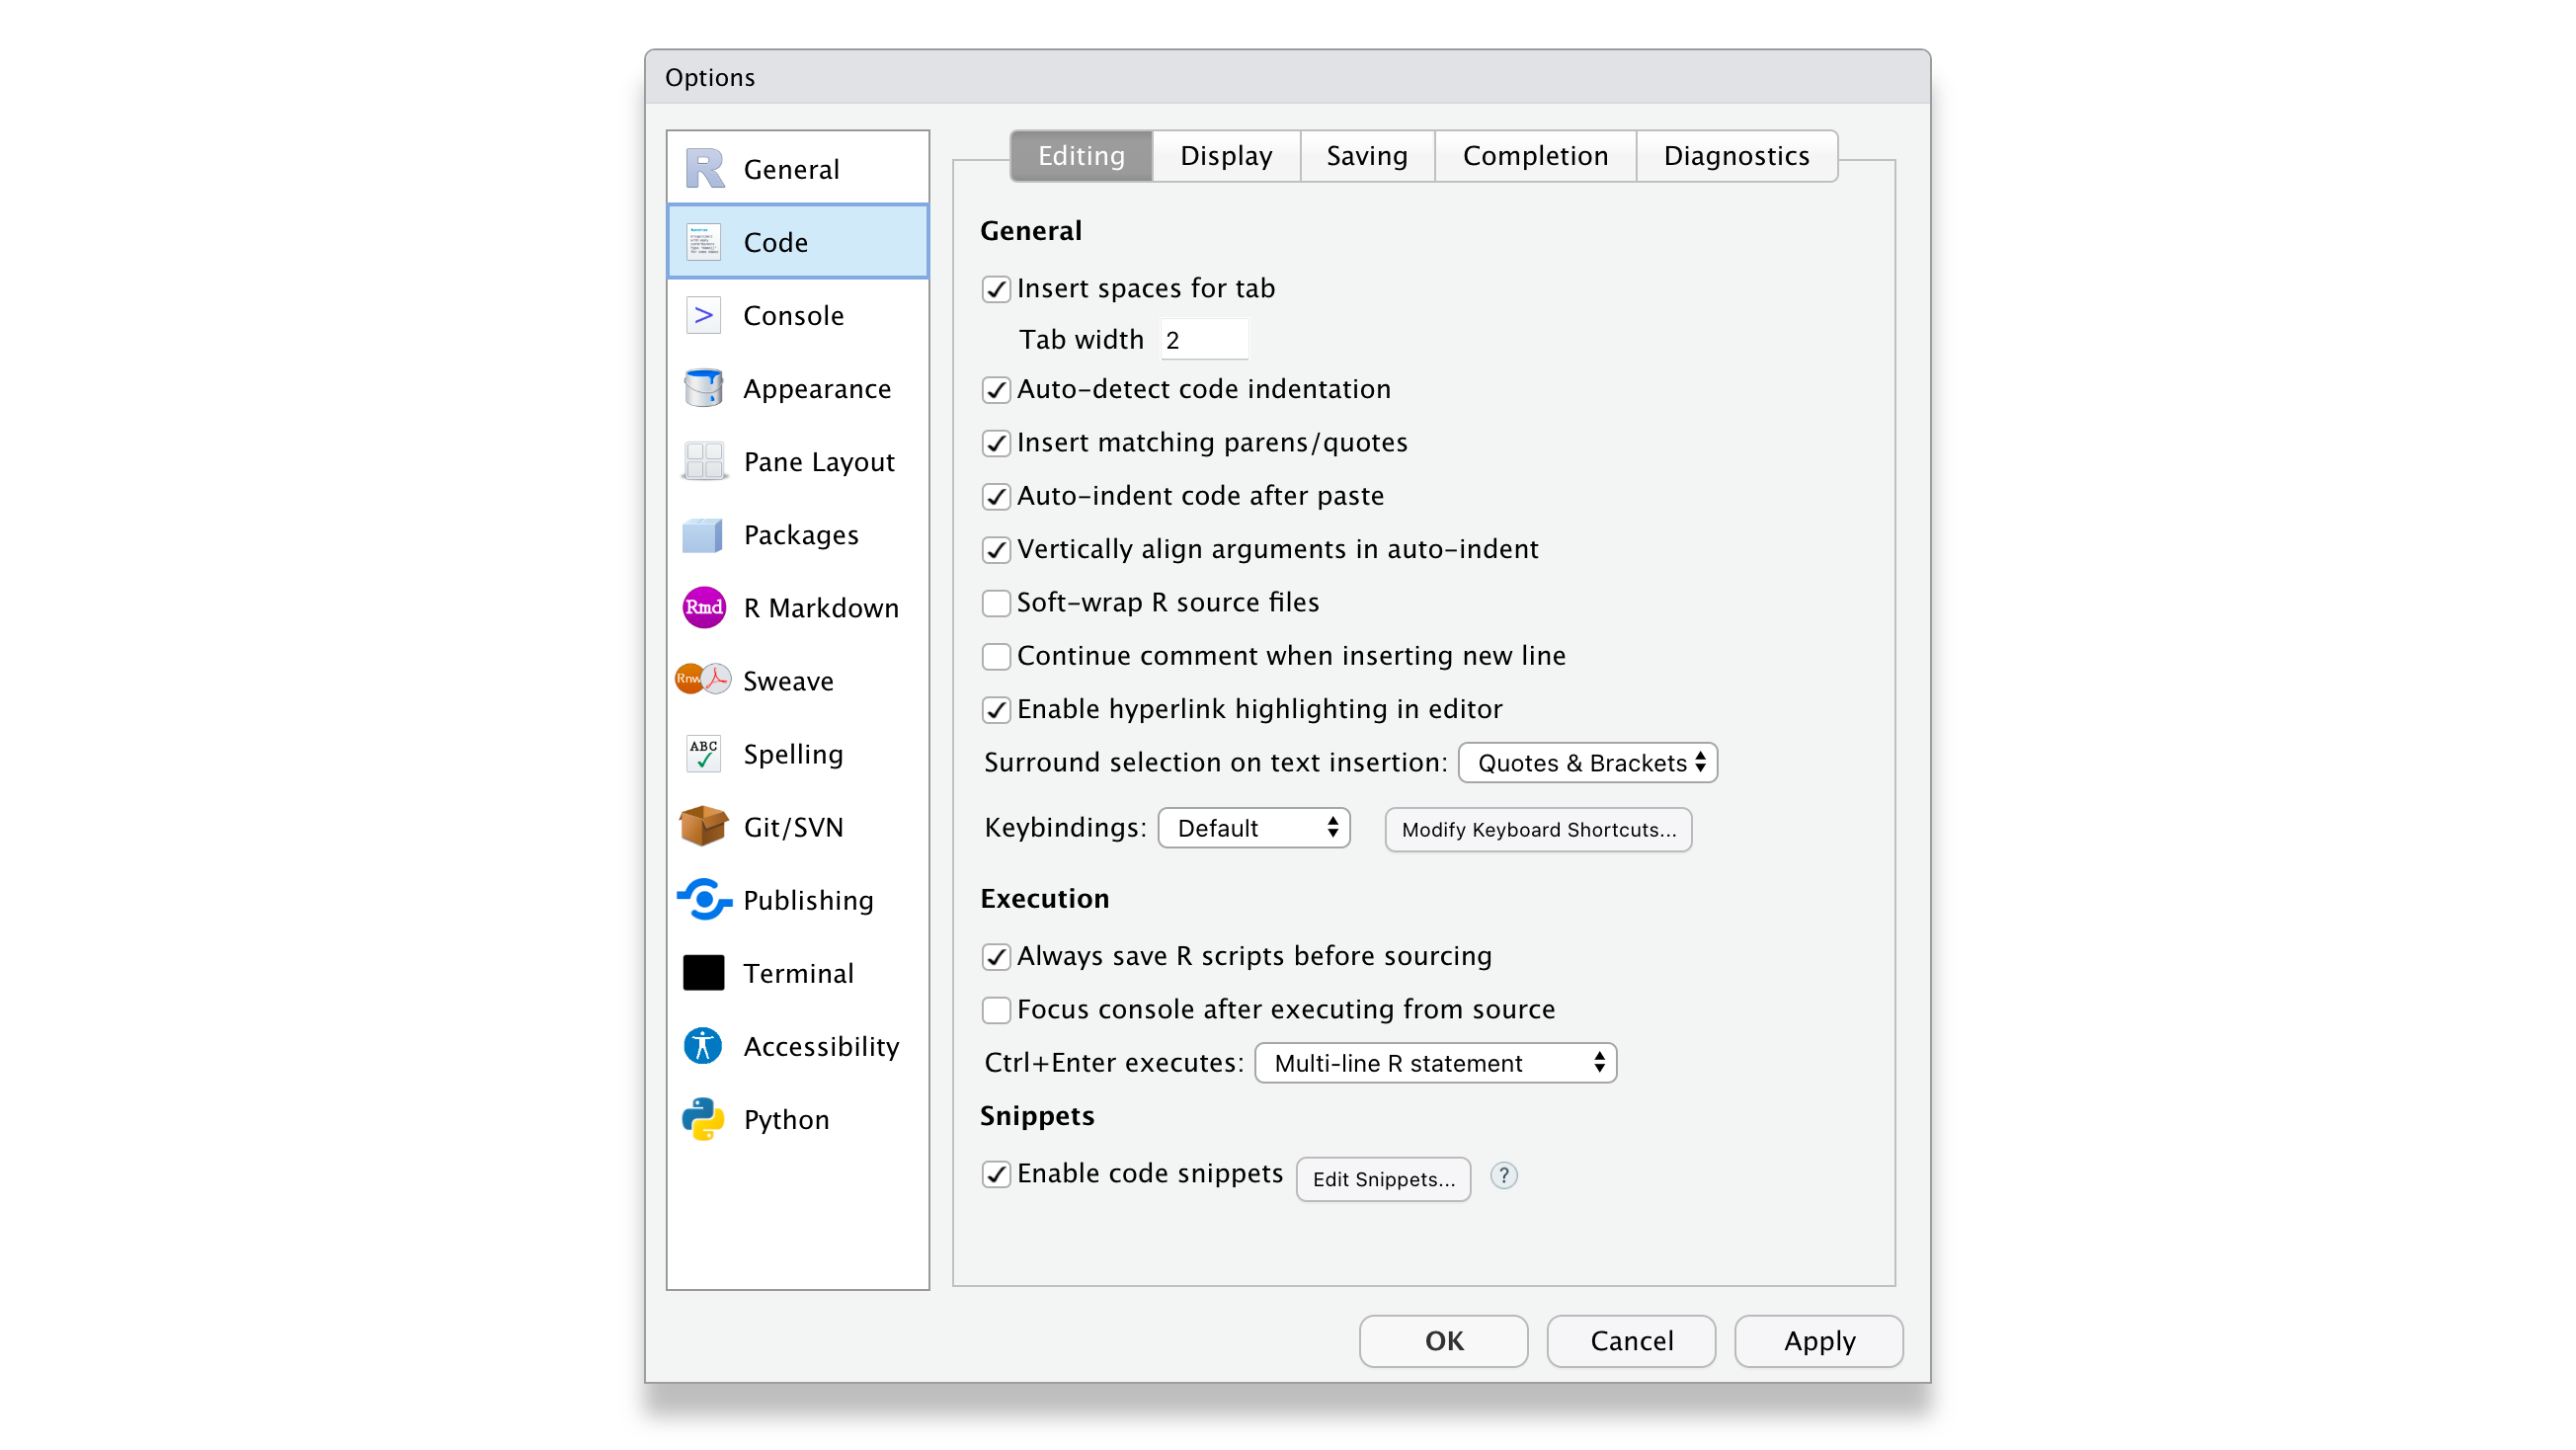
\includegraphics{images/chapter_03_img/rstudio_preferences/01_rstudio_preferences_editing.png}
\item
  In the \texttt{Display} tab, you might want to have the first three
  options selected. In particular, \texttt{Highlight\ selected\ line} is
  helpful because, in more complicated code, it is helpful to see where
  your cursor is.

  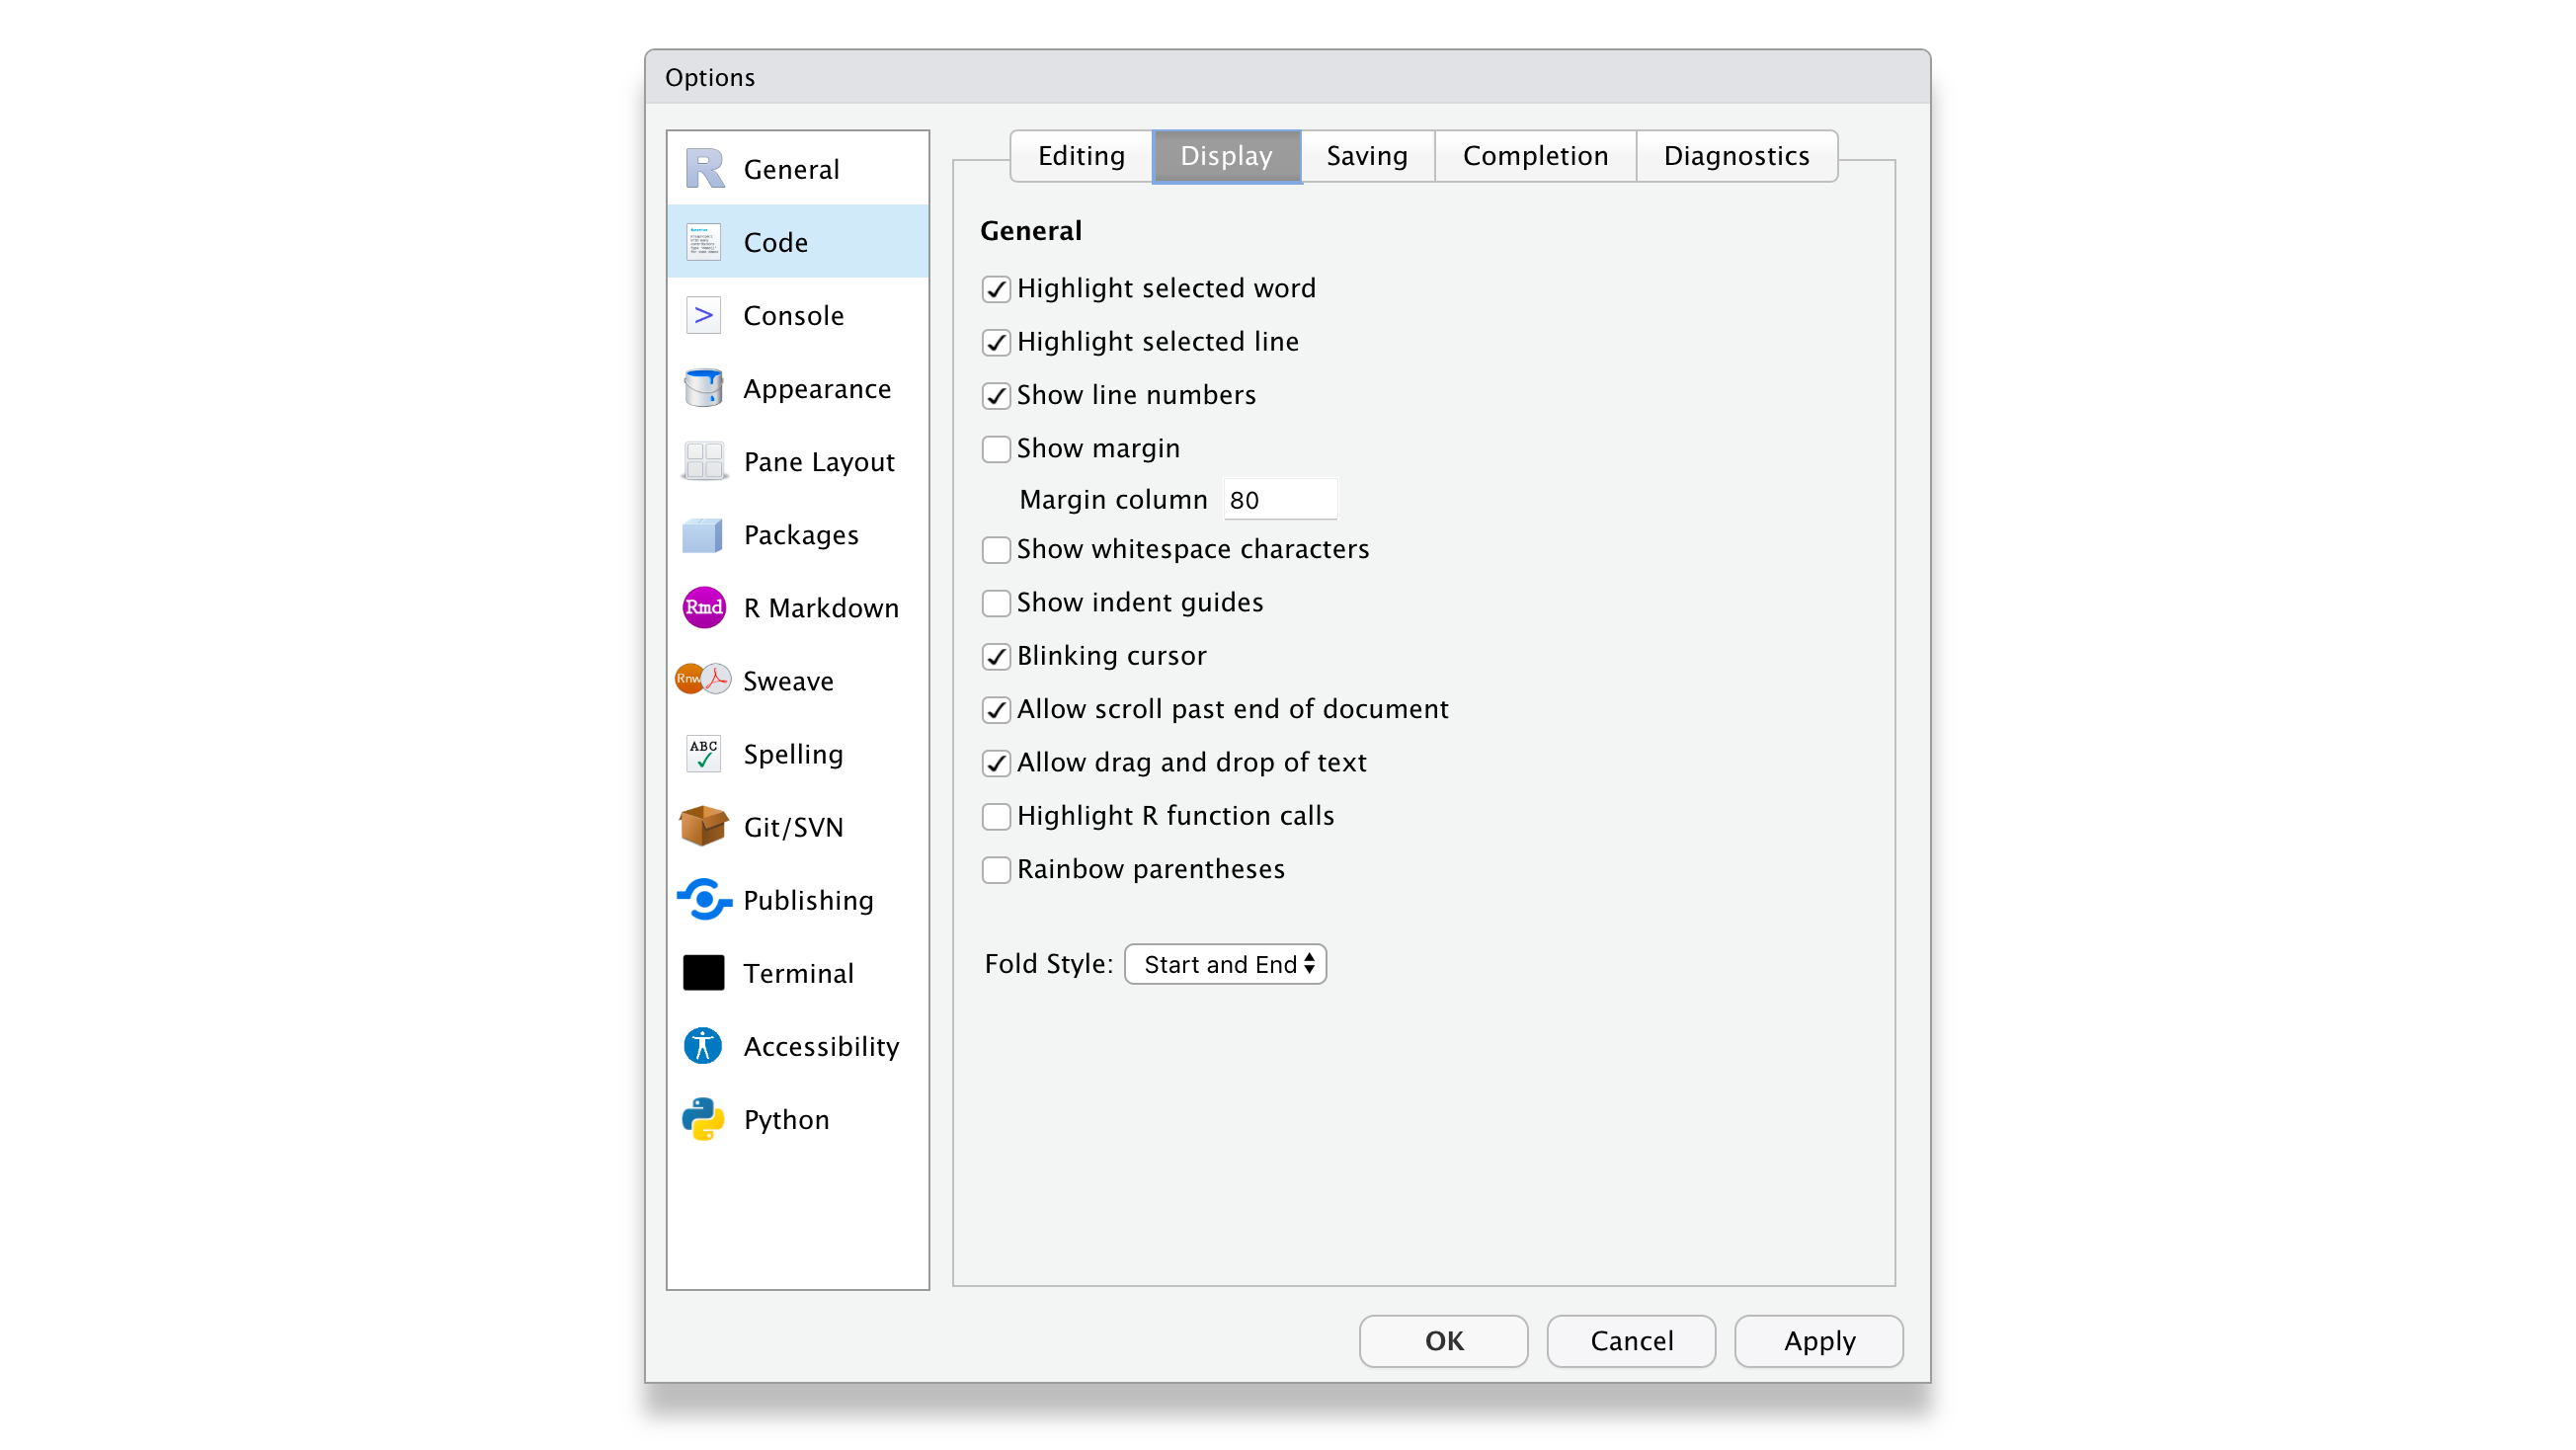
\includegraphics{images/chapter_03_img/rstudio_preferences/02_rstudio_preferences_display.png}
\end{enumerate}

Of course, if you wish to customise your workspace further, you can do
so. The visually most impactful way to alter the default appearance of
RStudio is to select \texttt{Appearance} and pick a completely different
colour theme. Feel free to browse through various options and see what
you prefer. There is no right or wrong here. Just make it your own.

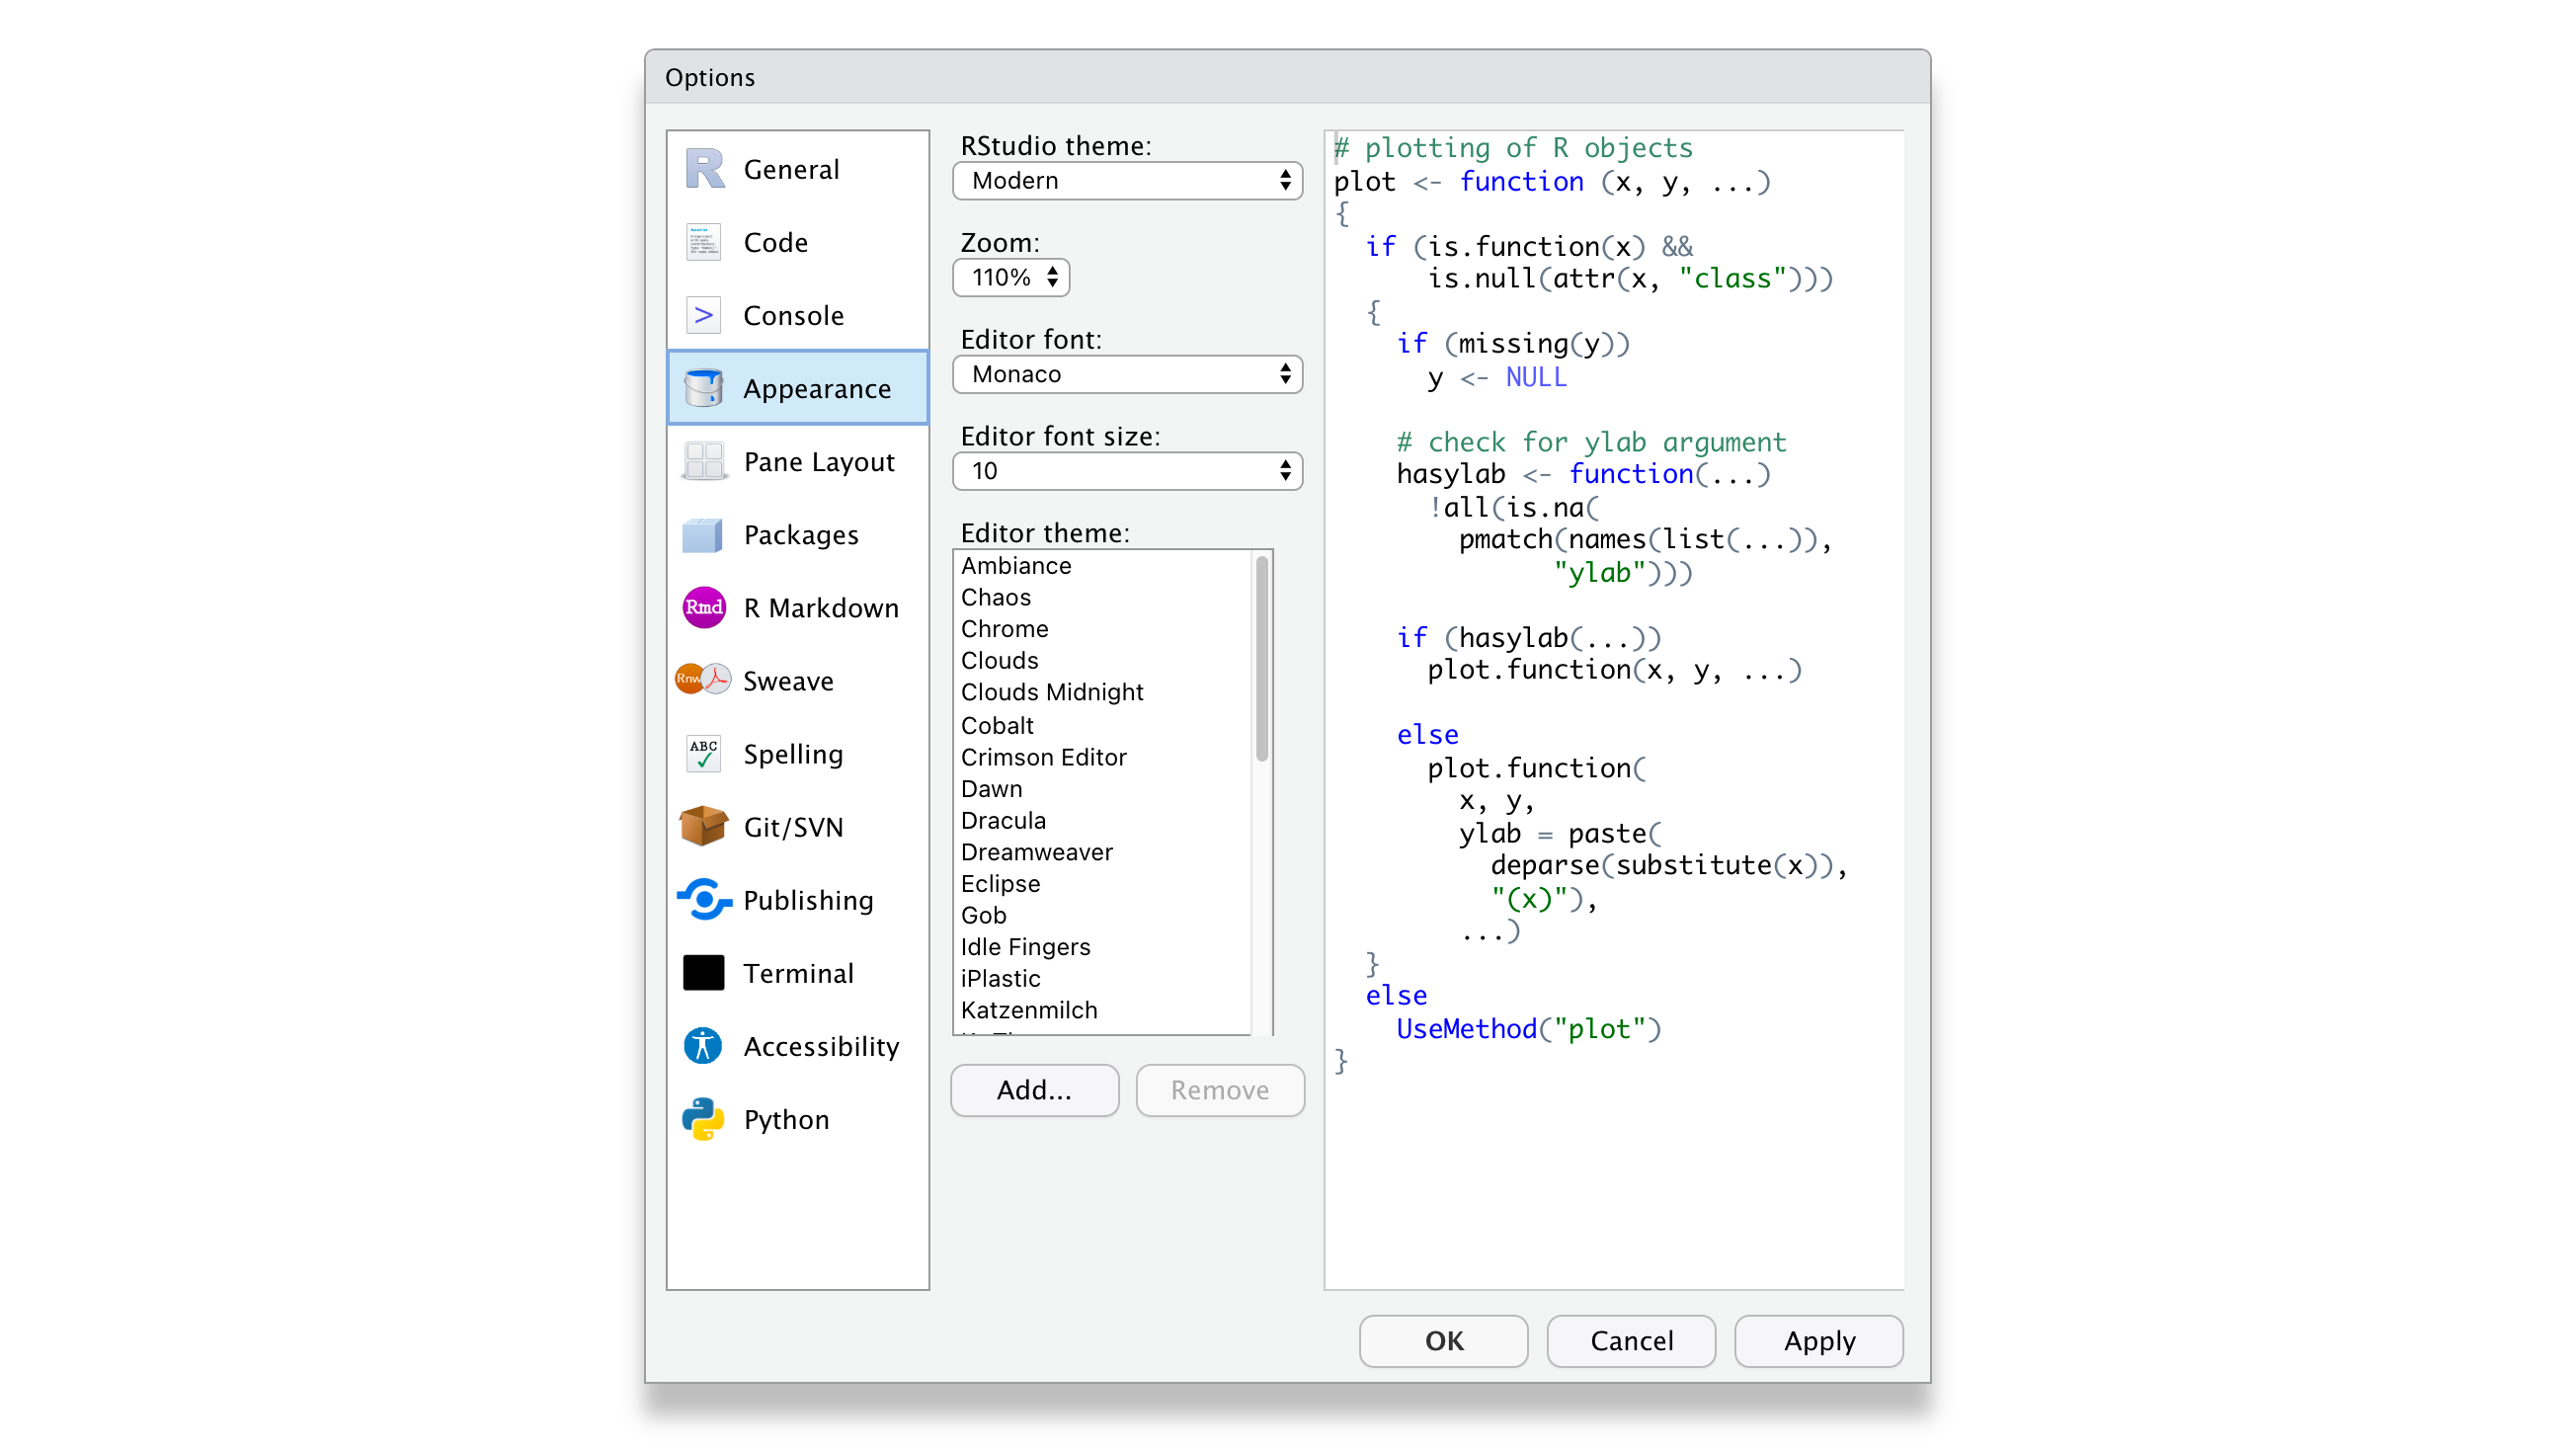
\includegraphics{images/chapter_03_img/rstudio_preferences/03_rstudio_preferences_appearance.png}

\section{\texorpdfstring{Updating \emph{R} and RStudio: Living at the
pulse of
innovation}{Updating R and RStudio: Living at the pulse of innovation}}\label{sec-updating-r-and-rstudio}

While not strictly something that helps you become a better programmer,
this advice might come in handy to avoid turning into a frustrated
programmer. When you update your software, you need to update \emph{R}
and RStudio separately from each other. While both \emph{R} and RStudio
work closely with each other, they still constitute separate pieces of
software. Thus, it is essential to remember that updating RStudio will
not automatically update \emph{R}. This can become problematic if
specific tools you installed via RStudio (like a fancy learning
algorithm) might not be compatible with earlier versions of \emph{R}.
Also, additional \emph{R} packages (see Section~\ref{sec-r-packages})
developed by other developers are separate pieces that require updating
too, independently from \emph{R} and RStudio.

I know what you are thinking: This already sounds complicated and
cumbersome. However, rest assured, we look at how you can easily update
all your packages with RStudio. Thus, all you need to remember is that
\emph{R} needs to be updated separately from everything else.

\section{Posit Cloud}\label{sec-rstudio-cloud}

Posit Cloud is an application that runs in your web browser. It allows
you to write and access \emph{R} code wherever you go. It even works on
your tablet because it does not require installation. However, do expect
it to run slower if your internet connection is not fast or stable. To
work with Posit Cloud, you also need an internet connection. However,
there are many benefits to using RStudio in the cloud, such as running
time-consuming scripts without using your own device. Also, it is much
easier to collaborate with others, and since no installation is
required, you can work on projects on any device as long as you are
connected to the internet. However, Posit Cloud's most significant
advantage is that you can get started with programming within seconds
compared to a desktop installation. Still, I prefer my locally run
offline version of RStudio because I appreciate working offline as much
as online. Nevertheless, I recommend setting up an account because you
never know when you need it.

To get started with Posit Cloud, we have to undertake a couple of steps:

\begin{enumerate}
\def\labelenumi{\arabic{enumi}.}
\item
  Open your web browser of choice and navigate to
  \url{https://rstudio.cloud}.

  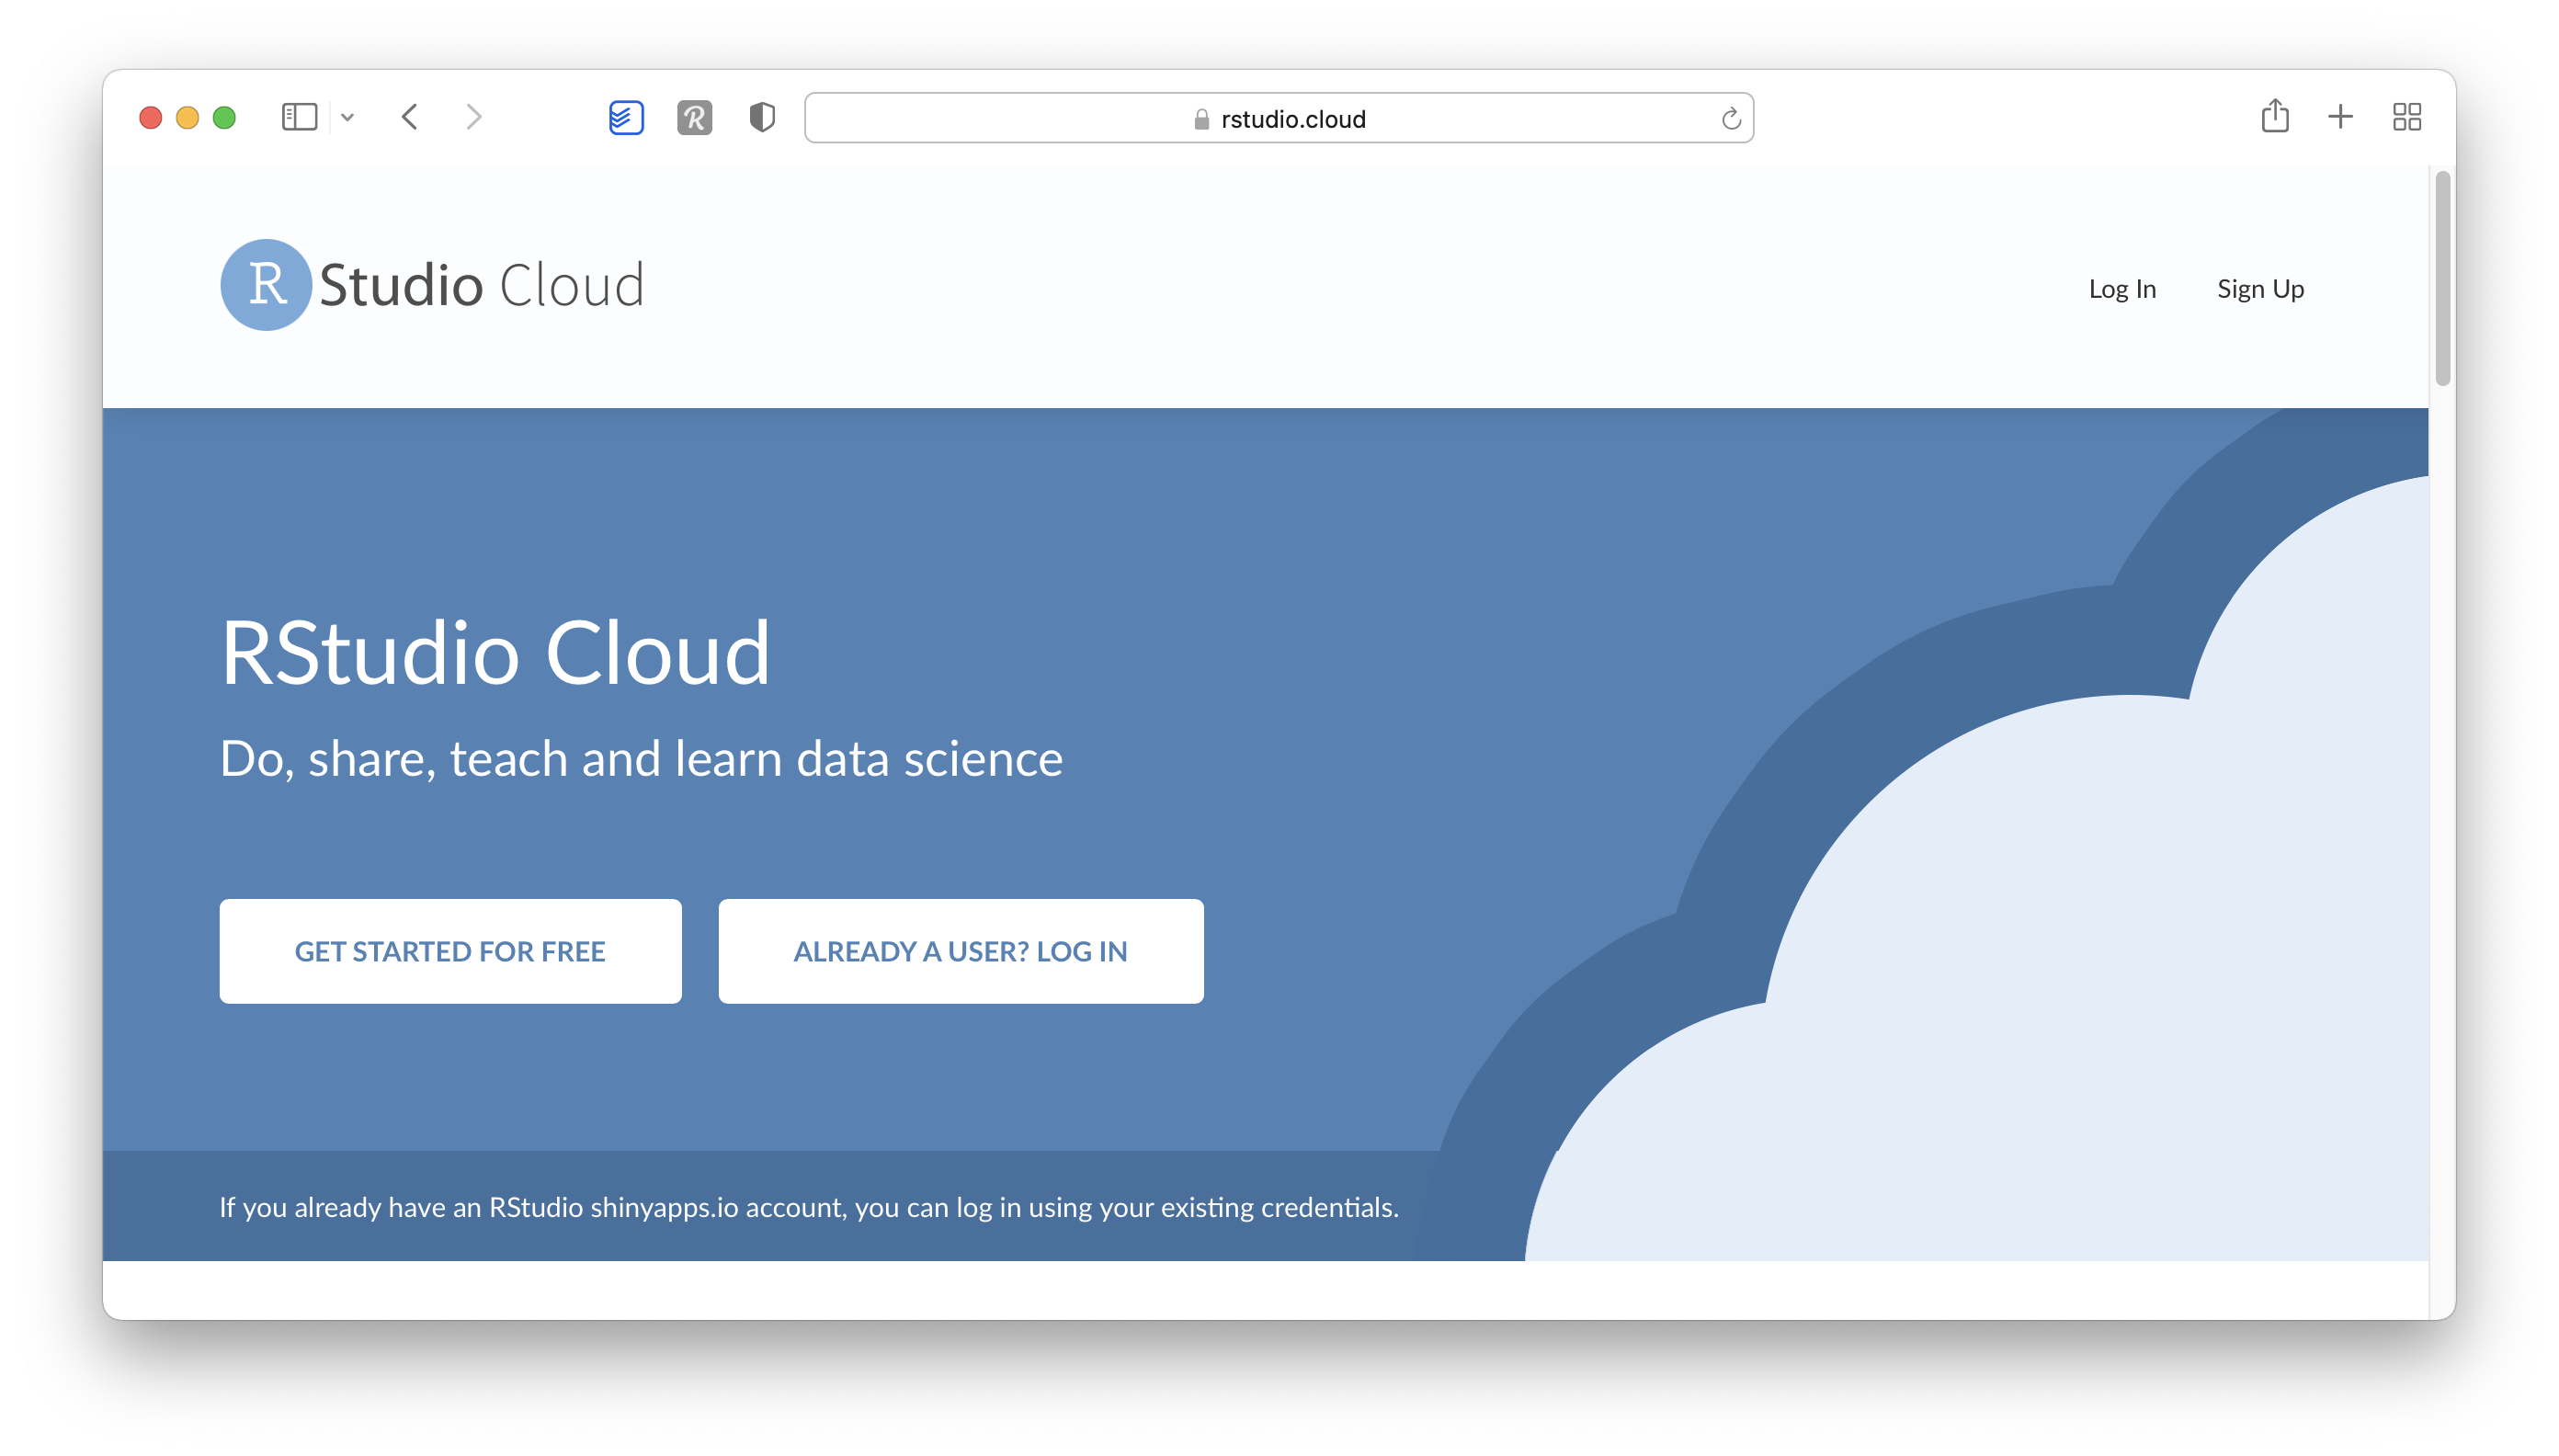
\includegraphics{images/chapter_03_img/rstudio_cloud/01_rstudio_cloud.png}
\item
  Click on \texttt{Sign\ Up} to create your account.
\item
  On the next page, make sure you have the free plan selected and click
  on \texttt{Sign\ up}.

  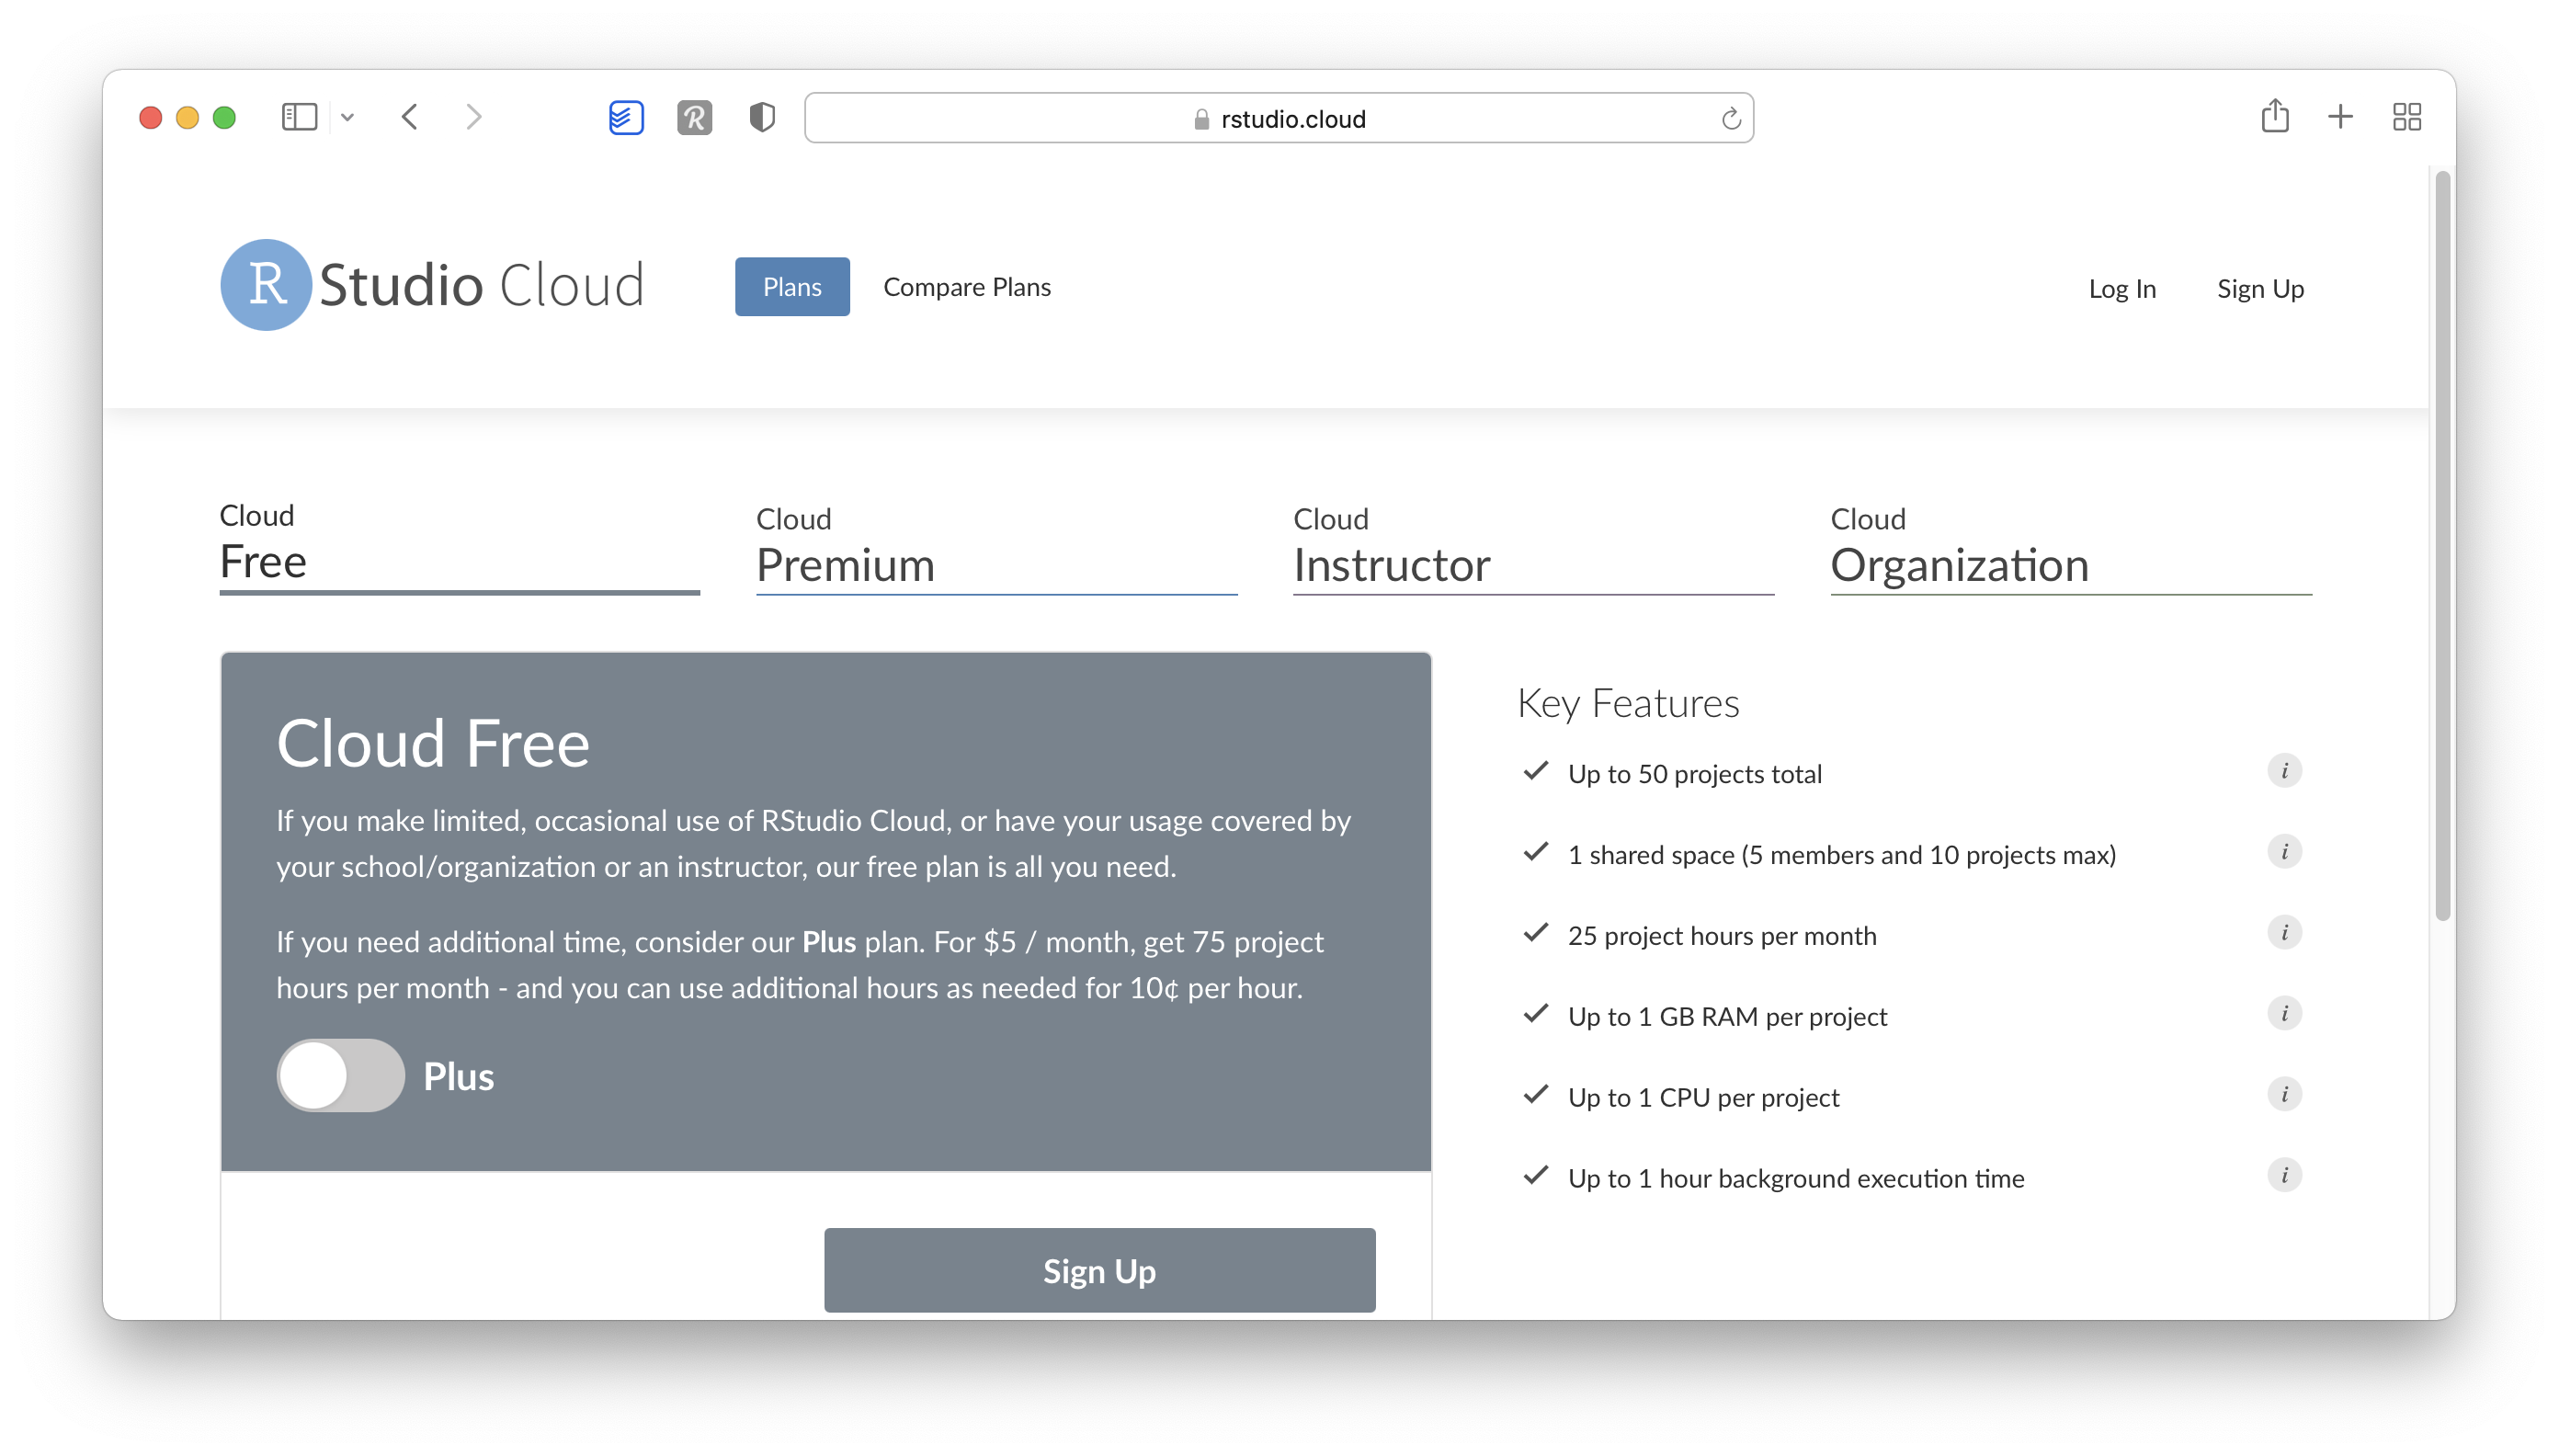
\includegraphics{images/chapter_03_img/rstudio_cloud/02_rstudio_cloud.png}
\item
  To finalise the registration process, you are required to provide your
  credentials.

  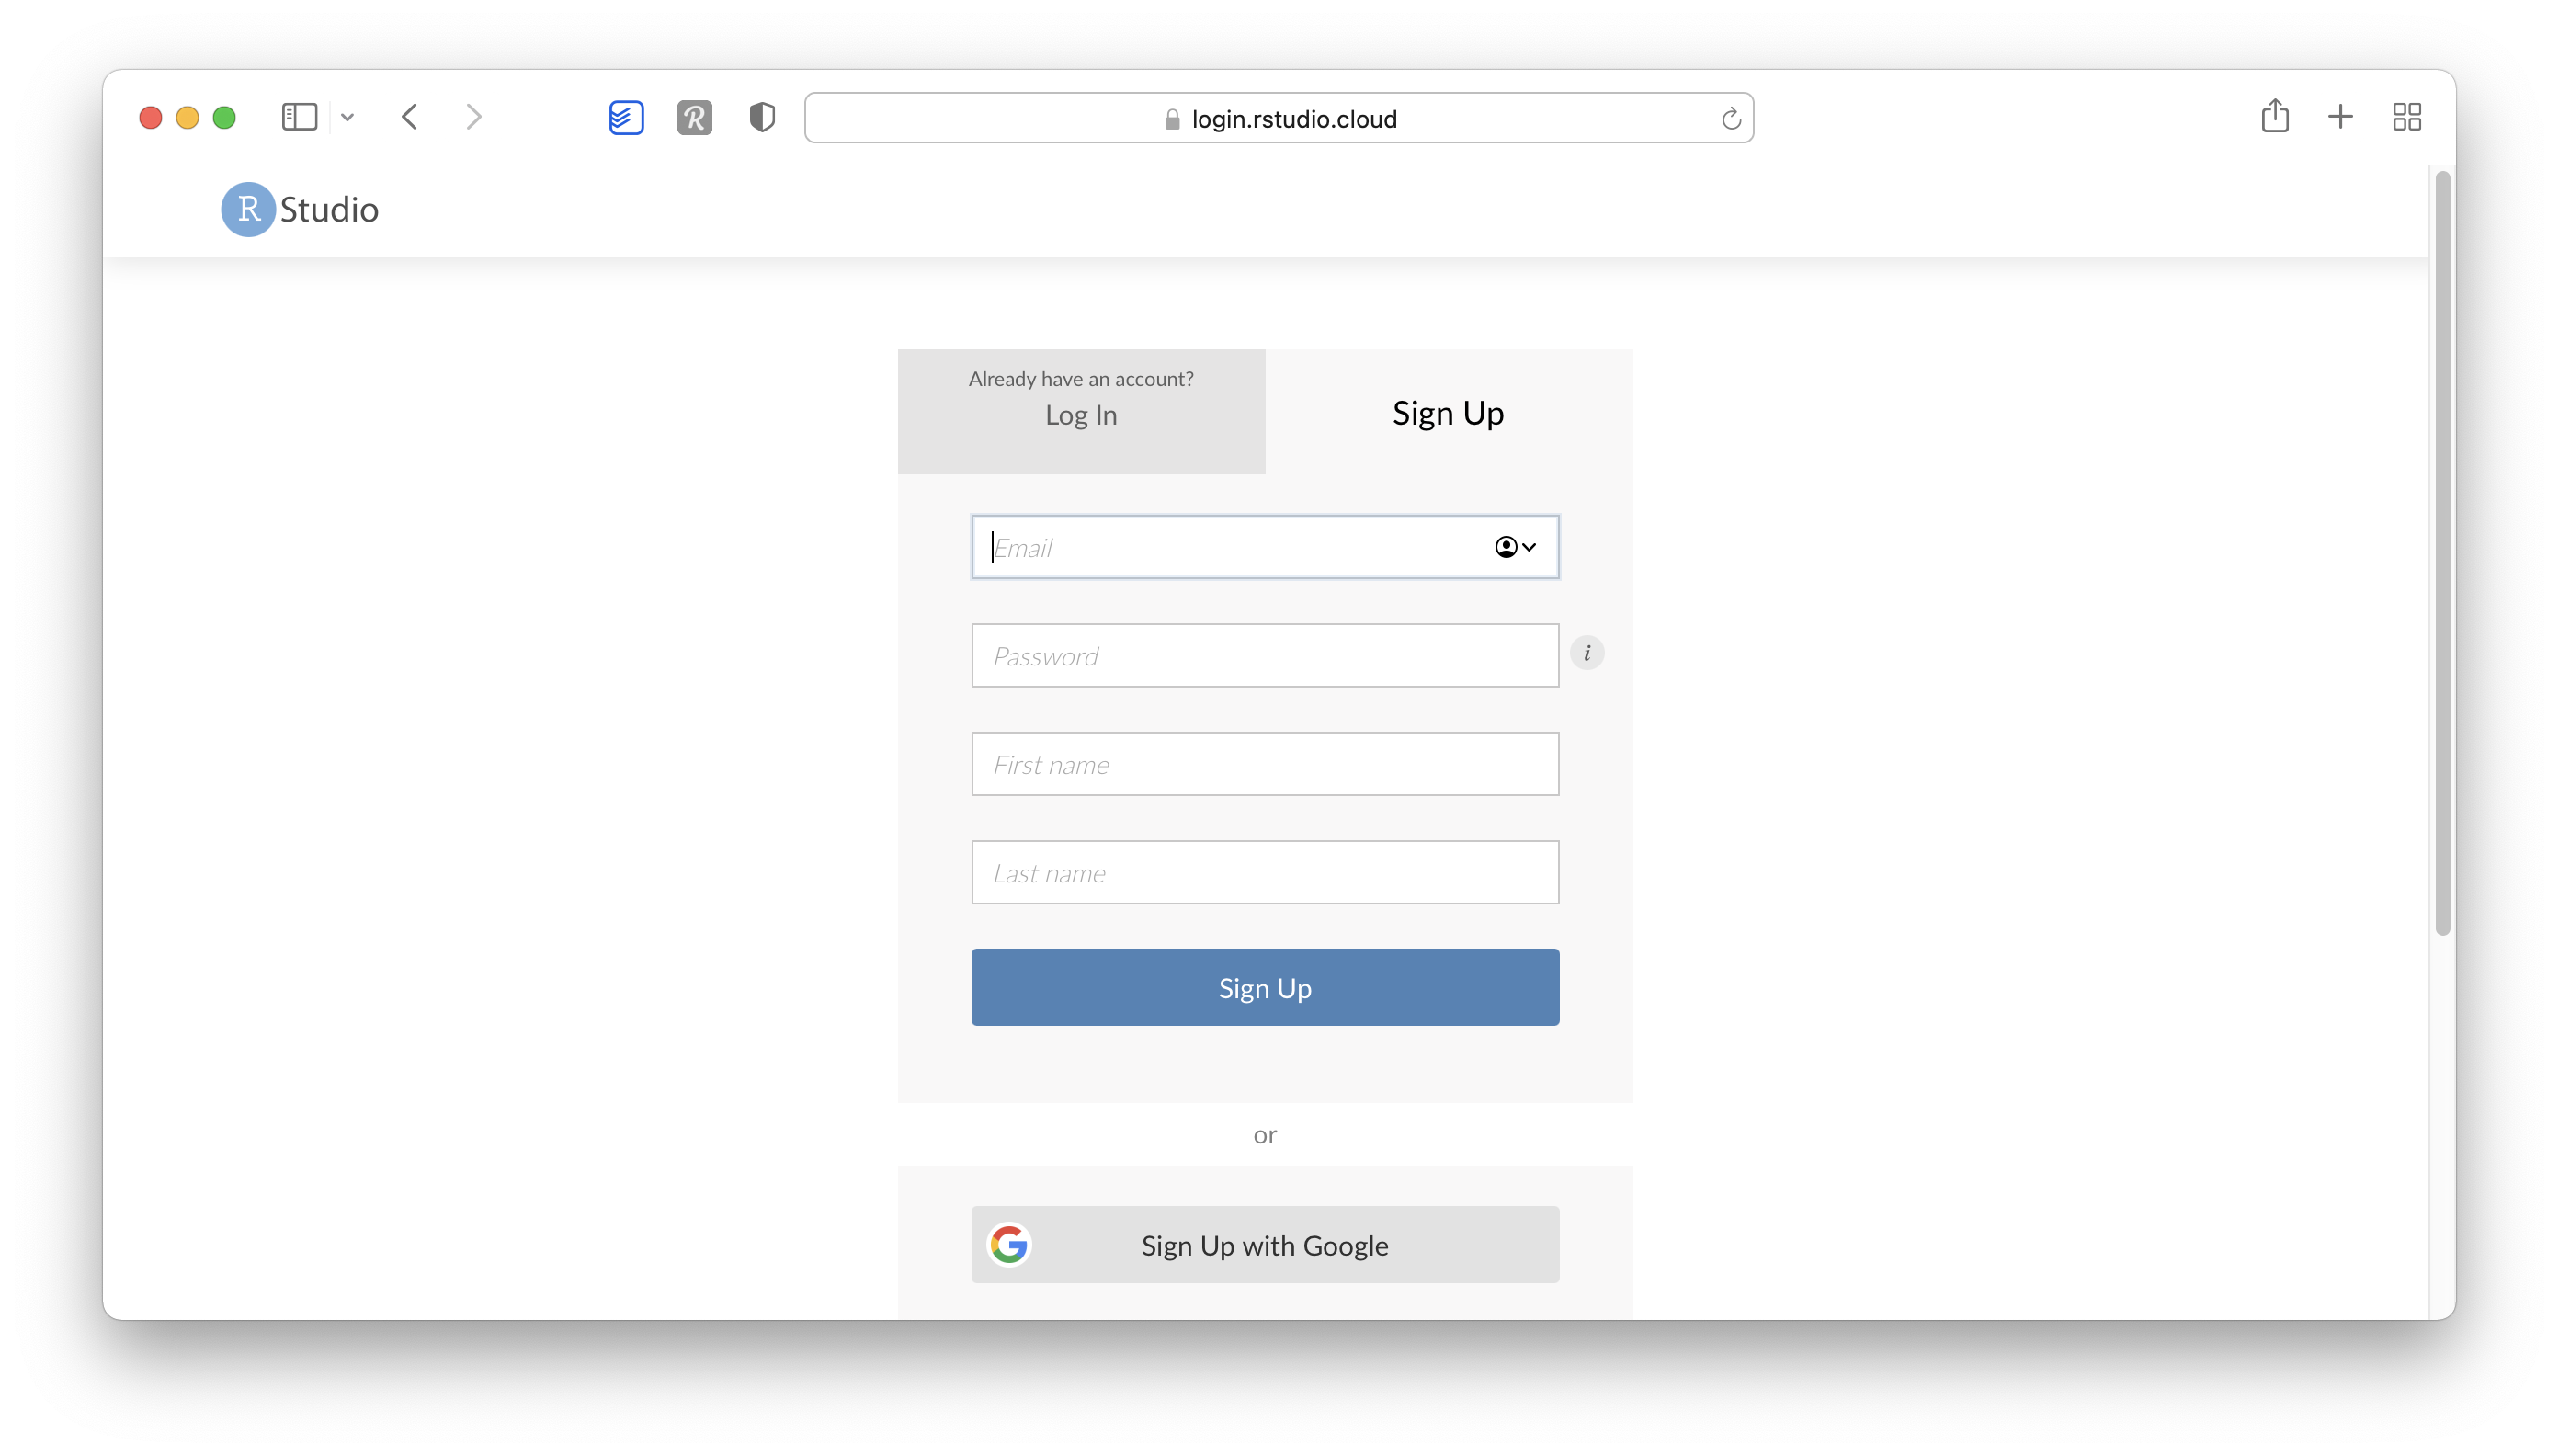
\includegraphics{images/chapter_03_img/rstudio_cloud/03_rstudio_cloud.png}
\item
  Once you complete your registration, you are redirected to
  \texttt{Your\ Workspace}, the central hub for all your projects. As
  you can tell, I already added another workspace called
  \texttt{R\ for\ Non-Programmers}. However, it is fine to use the
  default one.

  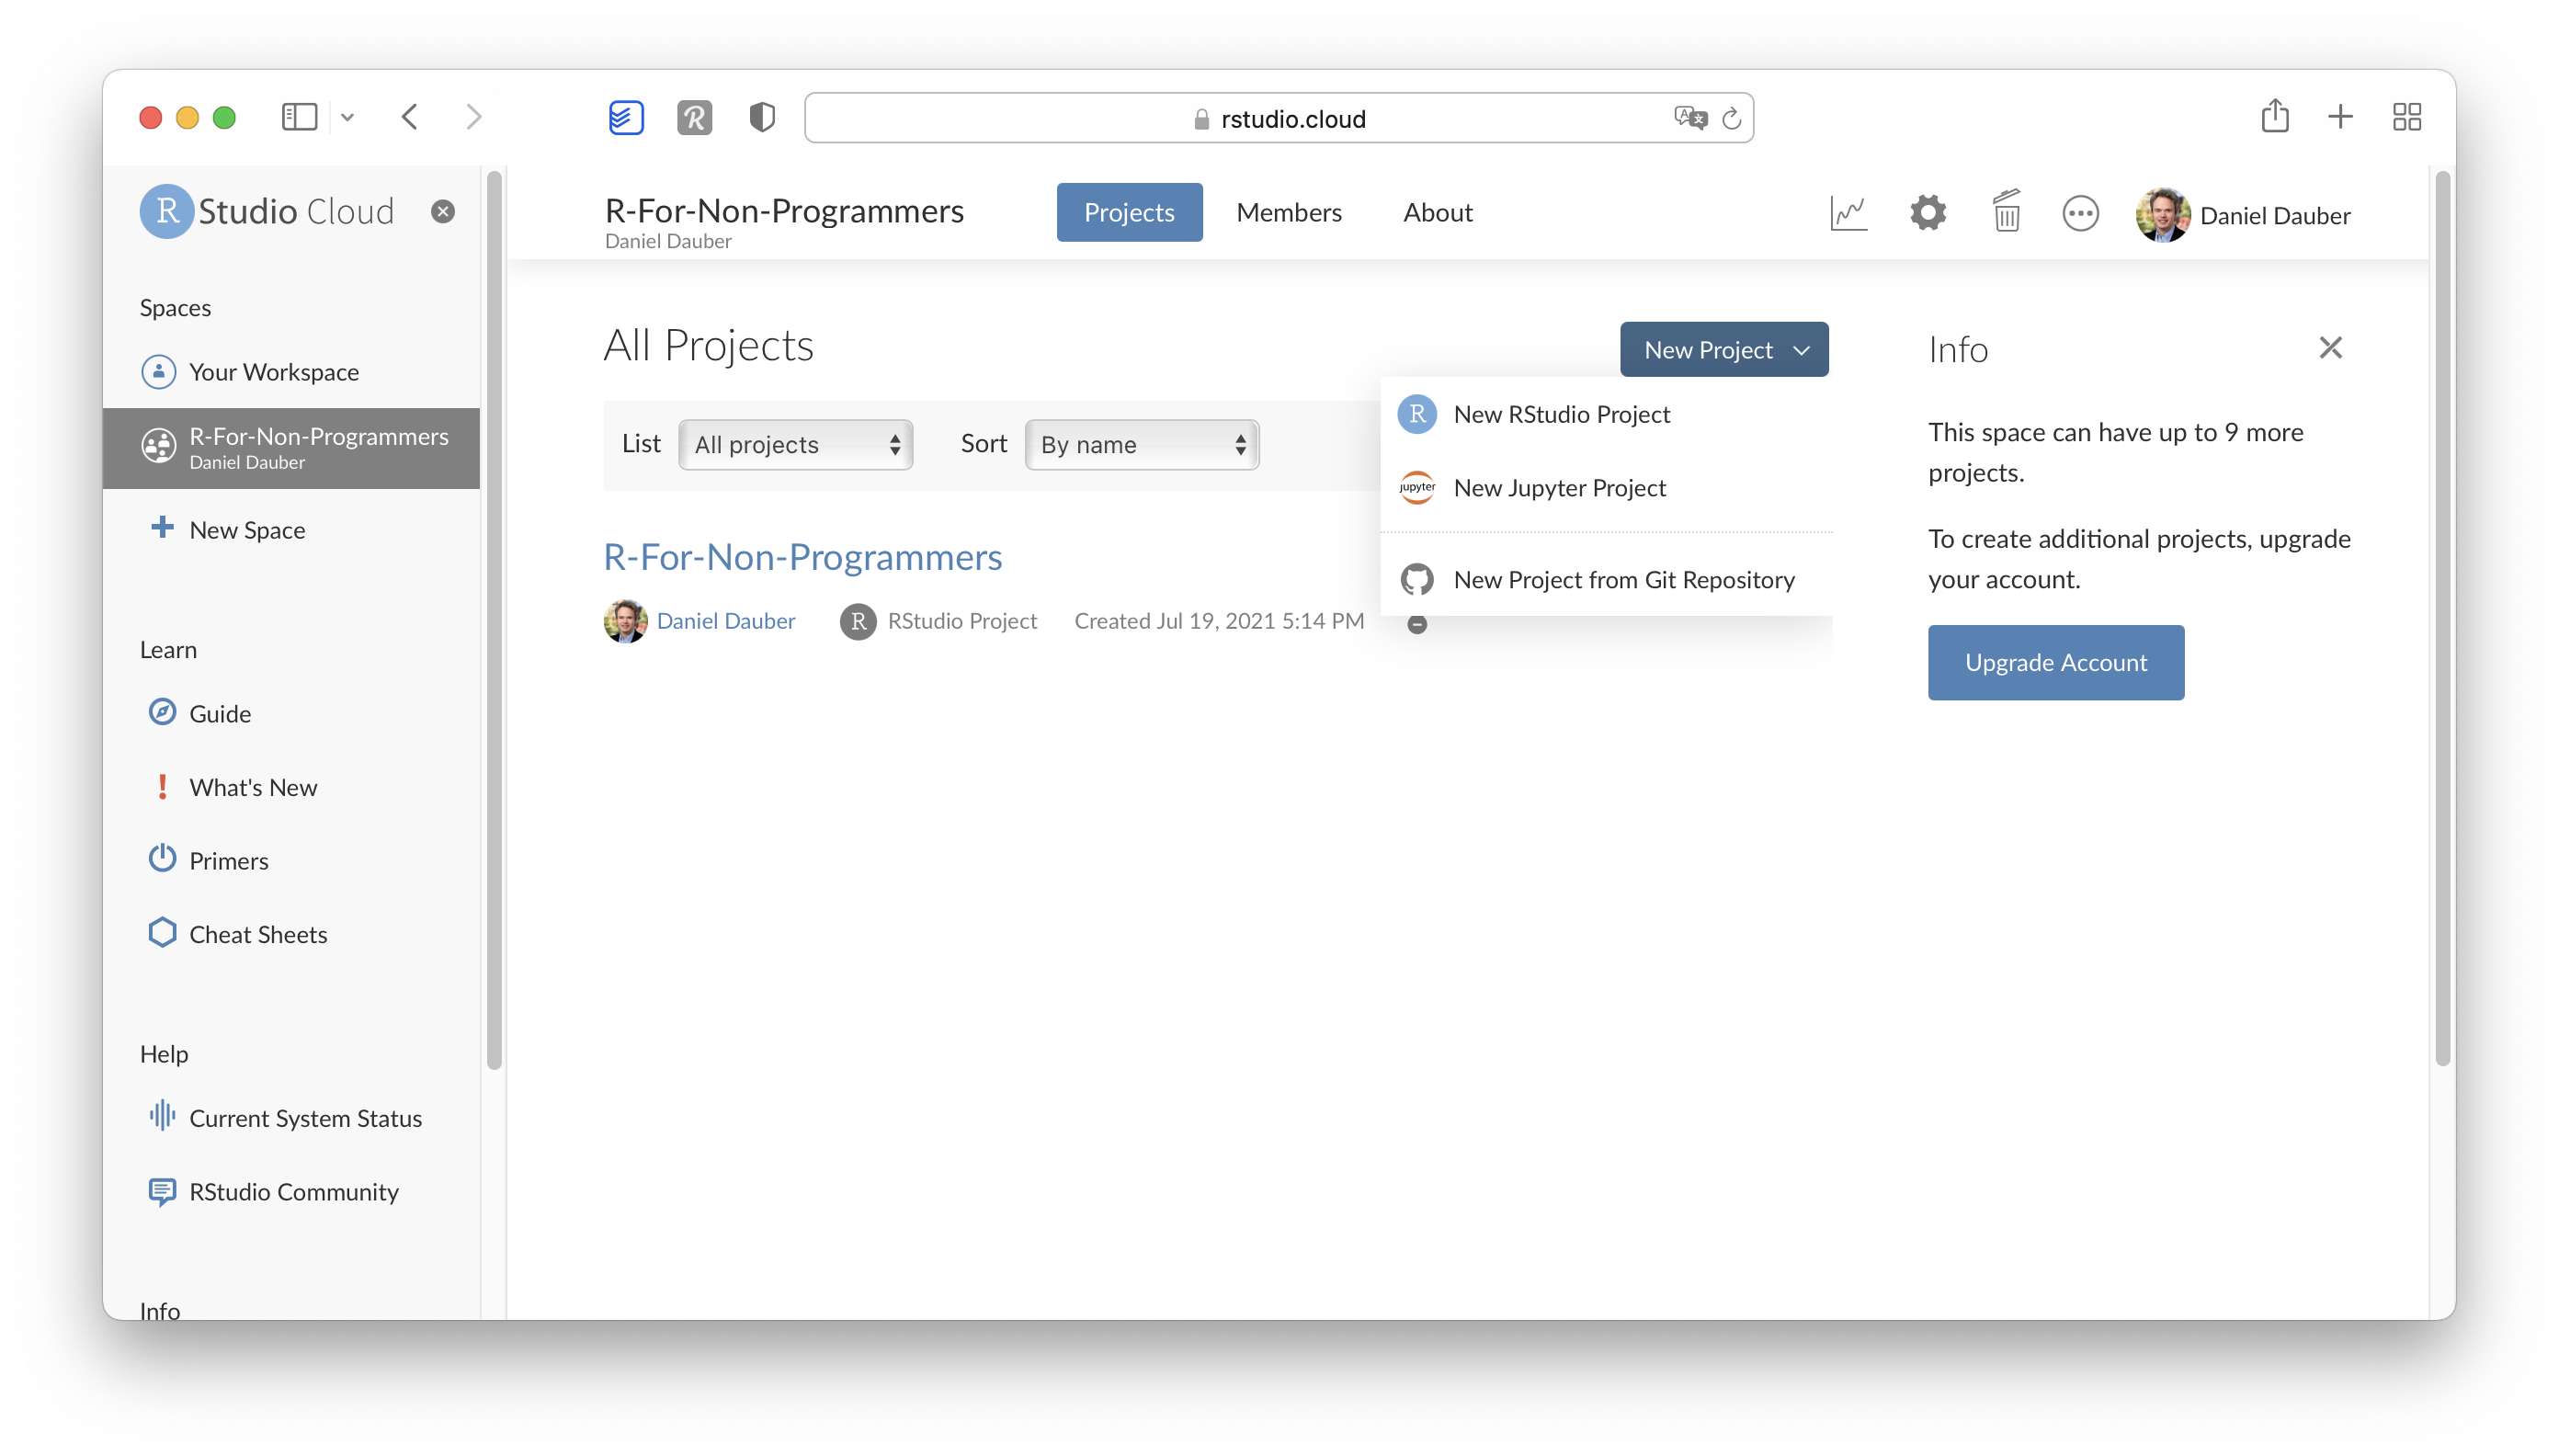
\includegraphics{images/chapter_03_img/rstudio_cloud/05_rstudio_cloud.png}
\item
  To start a new \emph{R} project, you can click on
  \texttt{New\ Project\ \textgreater{}\ New\ RStudio\ Project}. This
  will open RStudio in the Cloud, which looks identical to the desktop
  version. You can immediately start writing your code. The example
  below computes a plot.\footnote{RStudio and Posit Cloud warn you if
    you need to install certain \emph{R} packages to successfully run
    code. More about \emph{R} packages and what they are can be found in
    Section~\ref{sec-r-packages}.}

  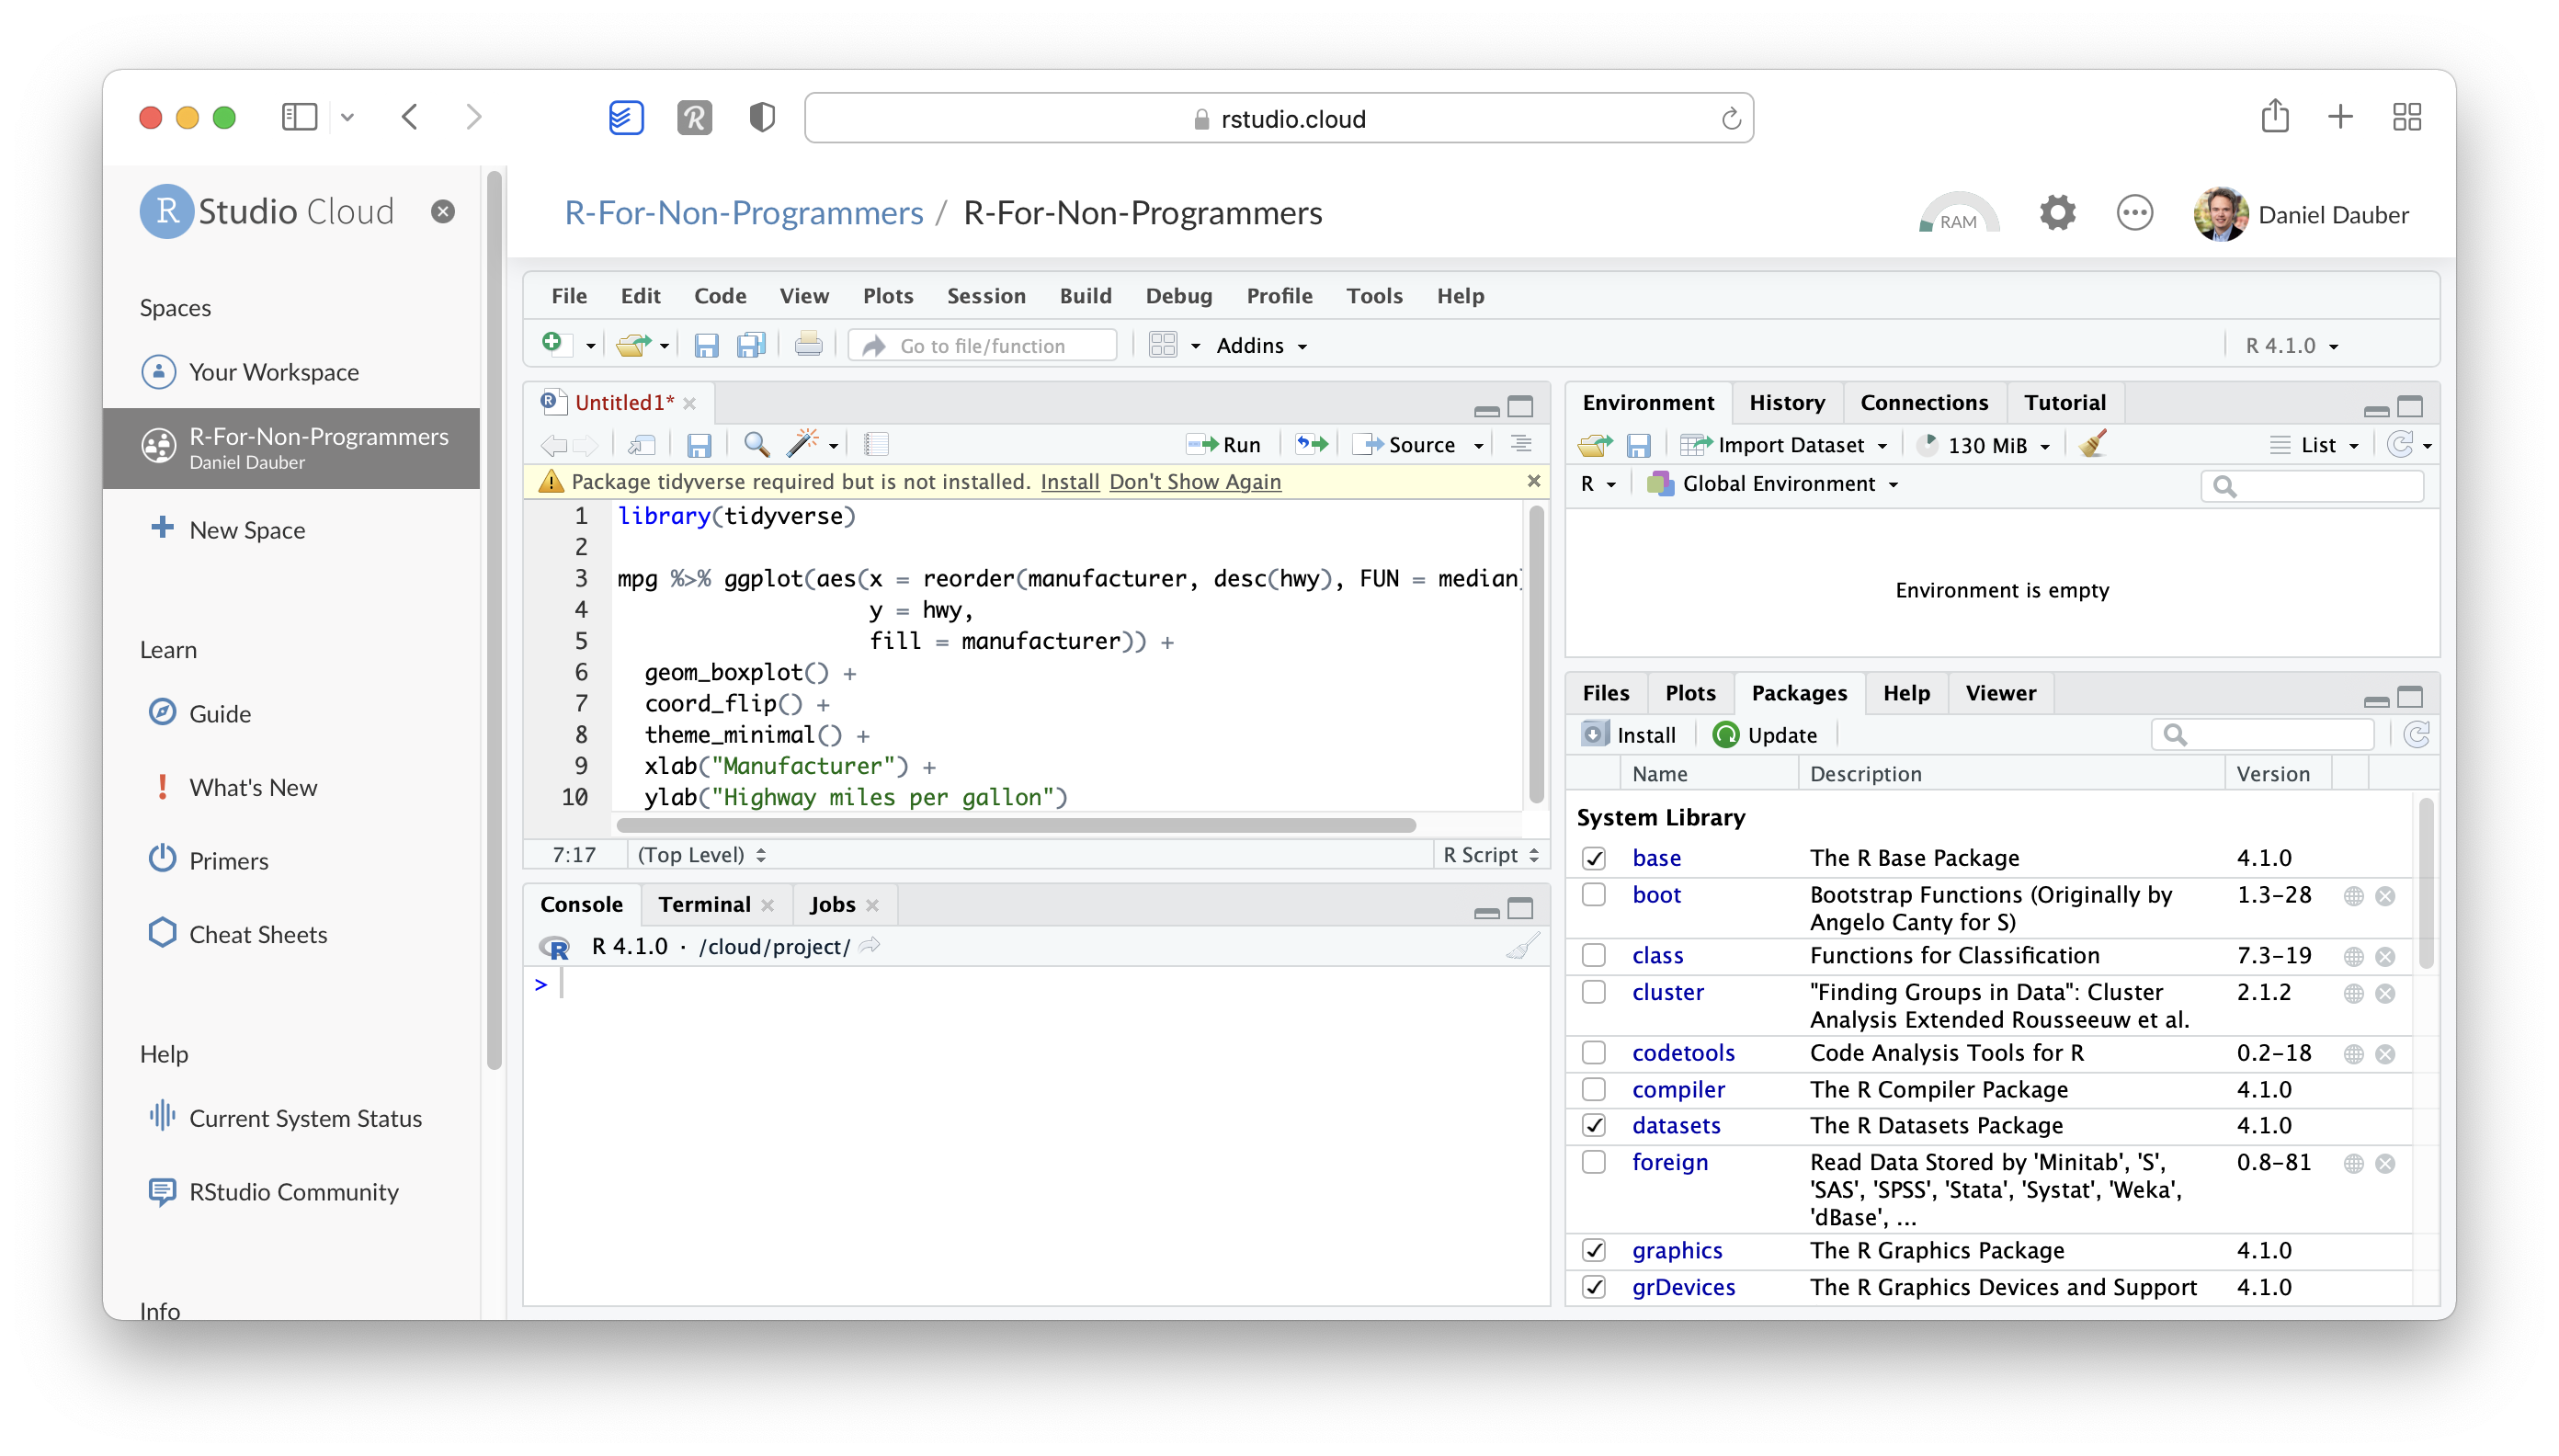
\includegraphics{images/chapter_03_img/rstudio_cloud/06_rstudio_cloud.png}
\item
  Now, we can execute the code as we would on the desktop version (see
  Chapter~\ref{sec-r-basics-the-very-fundamentals} ).

  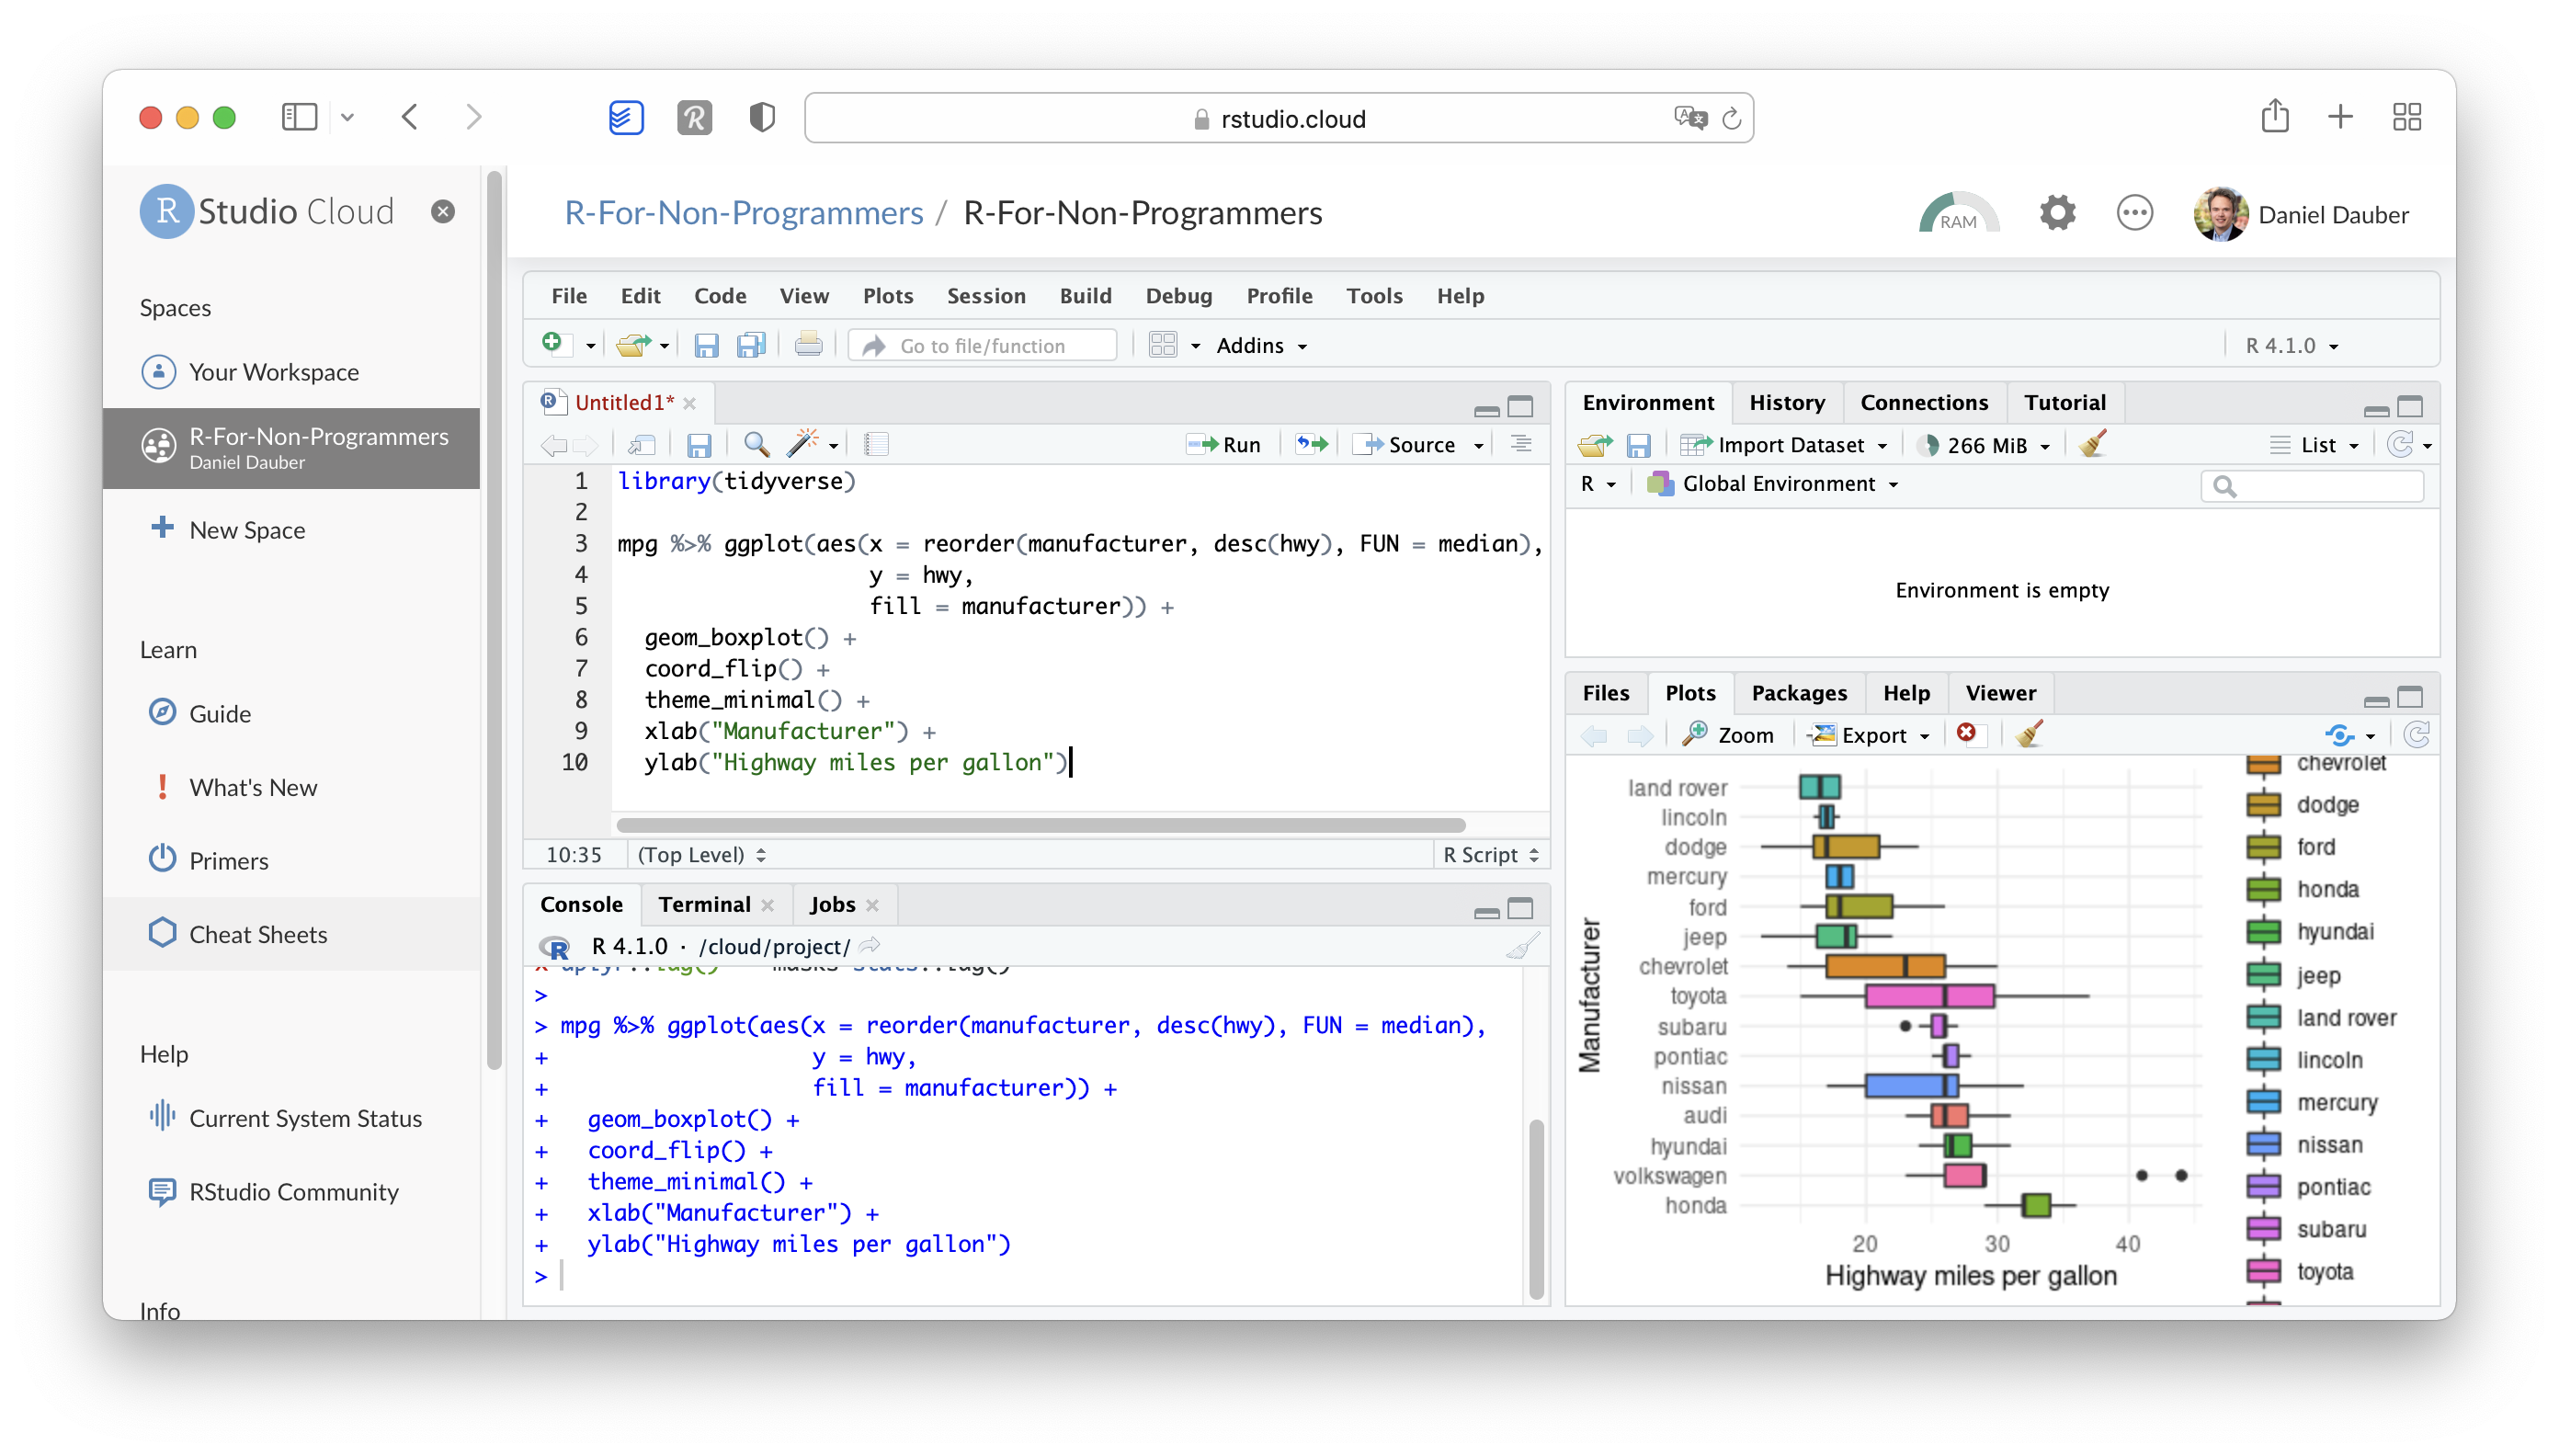
\includegraphics{images/chapter_03_img/rstudio_cloud/07_rstudio_cloud.png}
\end{enumerate}

Whether you choose to use a desktop version of RStudio or Posit Cloud,
you will be able to follow along in this book with no problem.

\bookmarksetup{startatroot}

\chapter{The RStudio Interface}\label{sec-the-rstudio-interface}

The RStudio interface is composed of quadrants, each of which fulfils a
unique purpose:

\begin{itemize}
\item
  The \texttt{Console} window,
\item
  The \texttt{Source} window,
\item
  The \texttt{Environment\ /\ History\ /\ Connections\ /\ Tutorial}
  window, and
\item
  The \texttt{Files\ /\ Plots\ /\ Packages\ /\ Help\ /\ Viewer} window
\end{itemize}

Sometimes, you might only see three windows and wonder where the
\texttt{Source} window has gone in your version of RStudio. In order to
use it, you have to either open a file or create a new one. You can
create a new file by selecting
\texttt{File\ \textgreater{}\ New\ File\ \textgreater{}\ R\ Script} in
the menu bar or using the keyboard shortcut
\texttt{Ctrl\ +\ Shift\ +\ N} on PC and \texttt{Cmd\ +\ Shift\ +\ N} on
Mac.

I will briefly explain the purpose of each window/pane and how they are
relevant to your work in \emph{R}.

\section{The Console window}\label{sec-the-console-window}

\begin{Shaded}
\begin{Highlighting}[]
\CommentTok{\# We type the below into the console}
\DecValTok{10} \SpecialCharTok{+} \DecValTok{5}
\end{Highlighting}
\end{Shaded}

\begin{verbatim}
[1] 15
\end{verbatim}

Here is a screenshot of how it should look like at your end in RStudio:

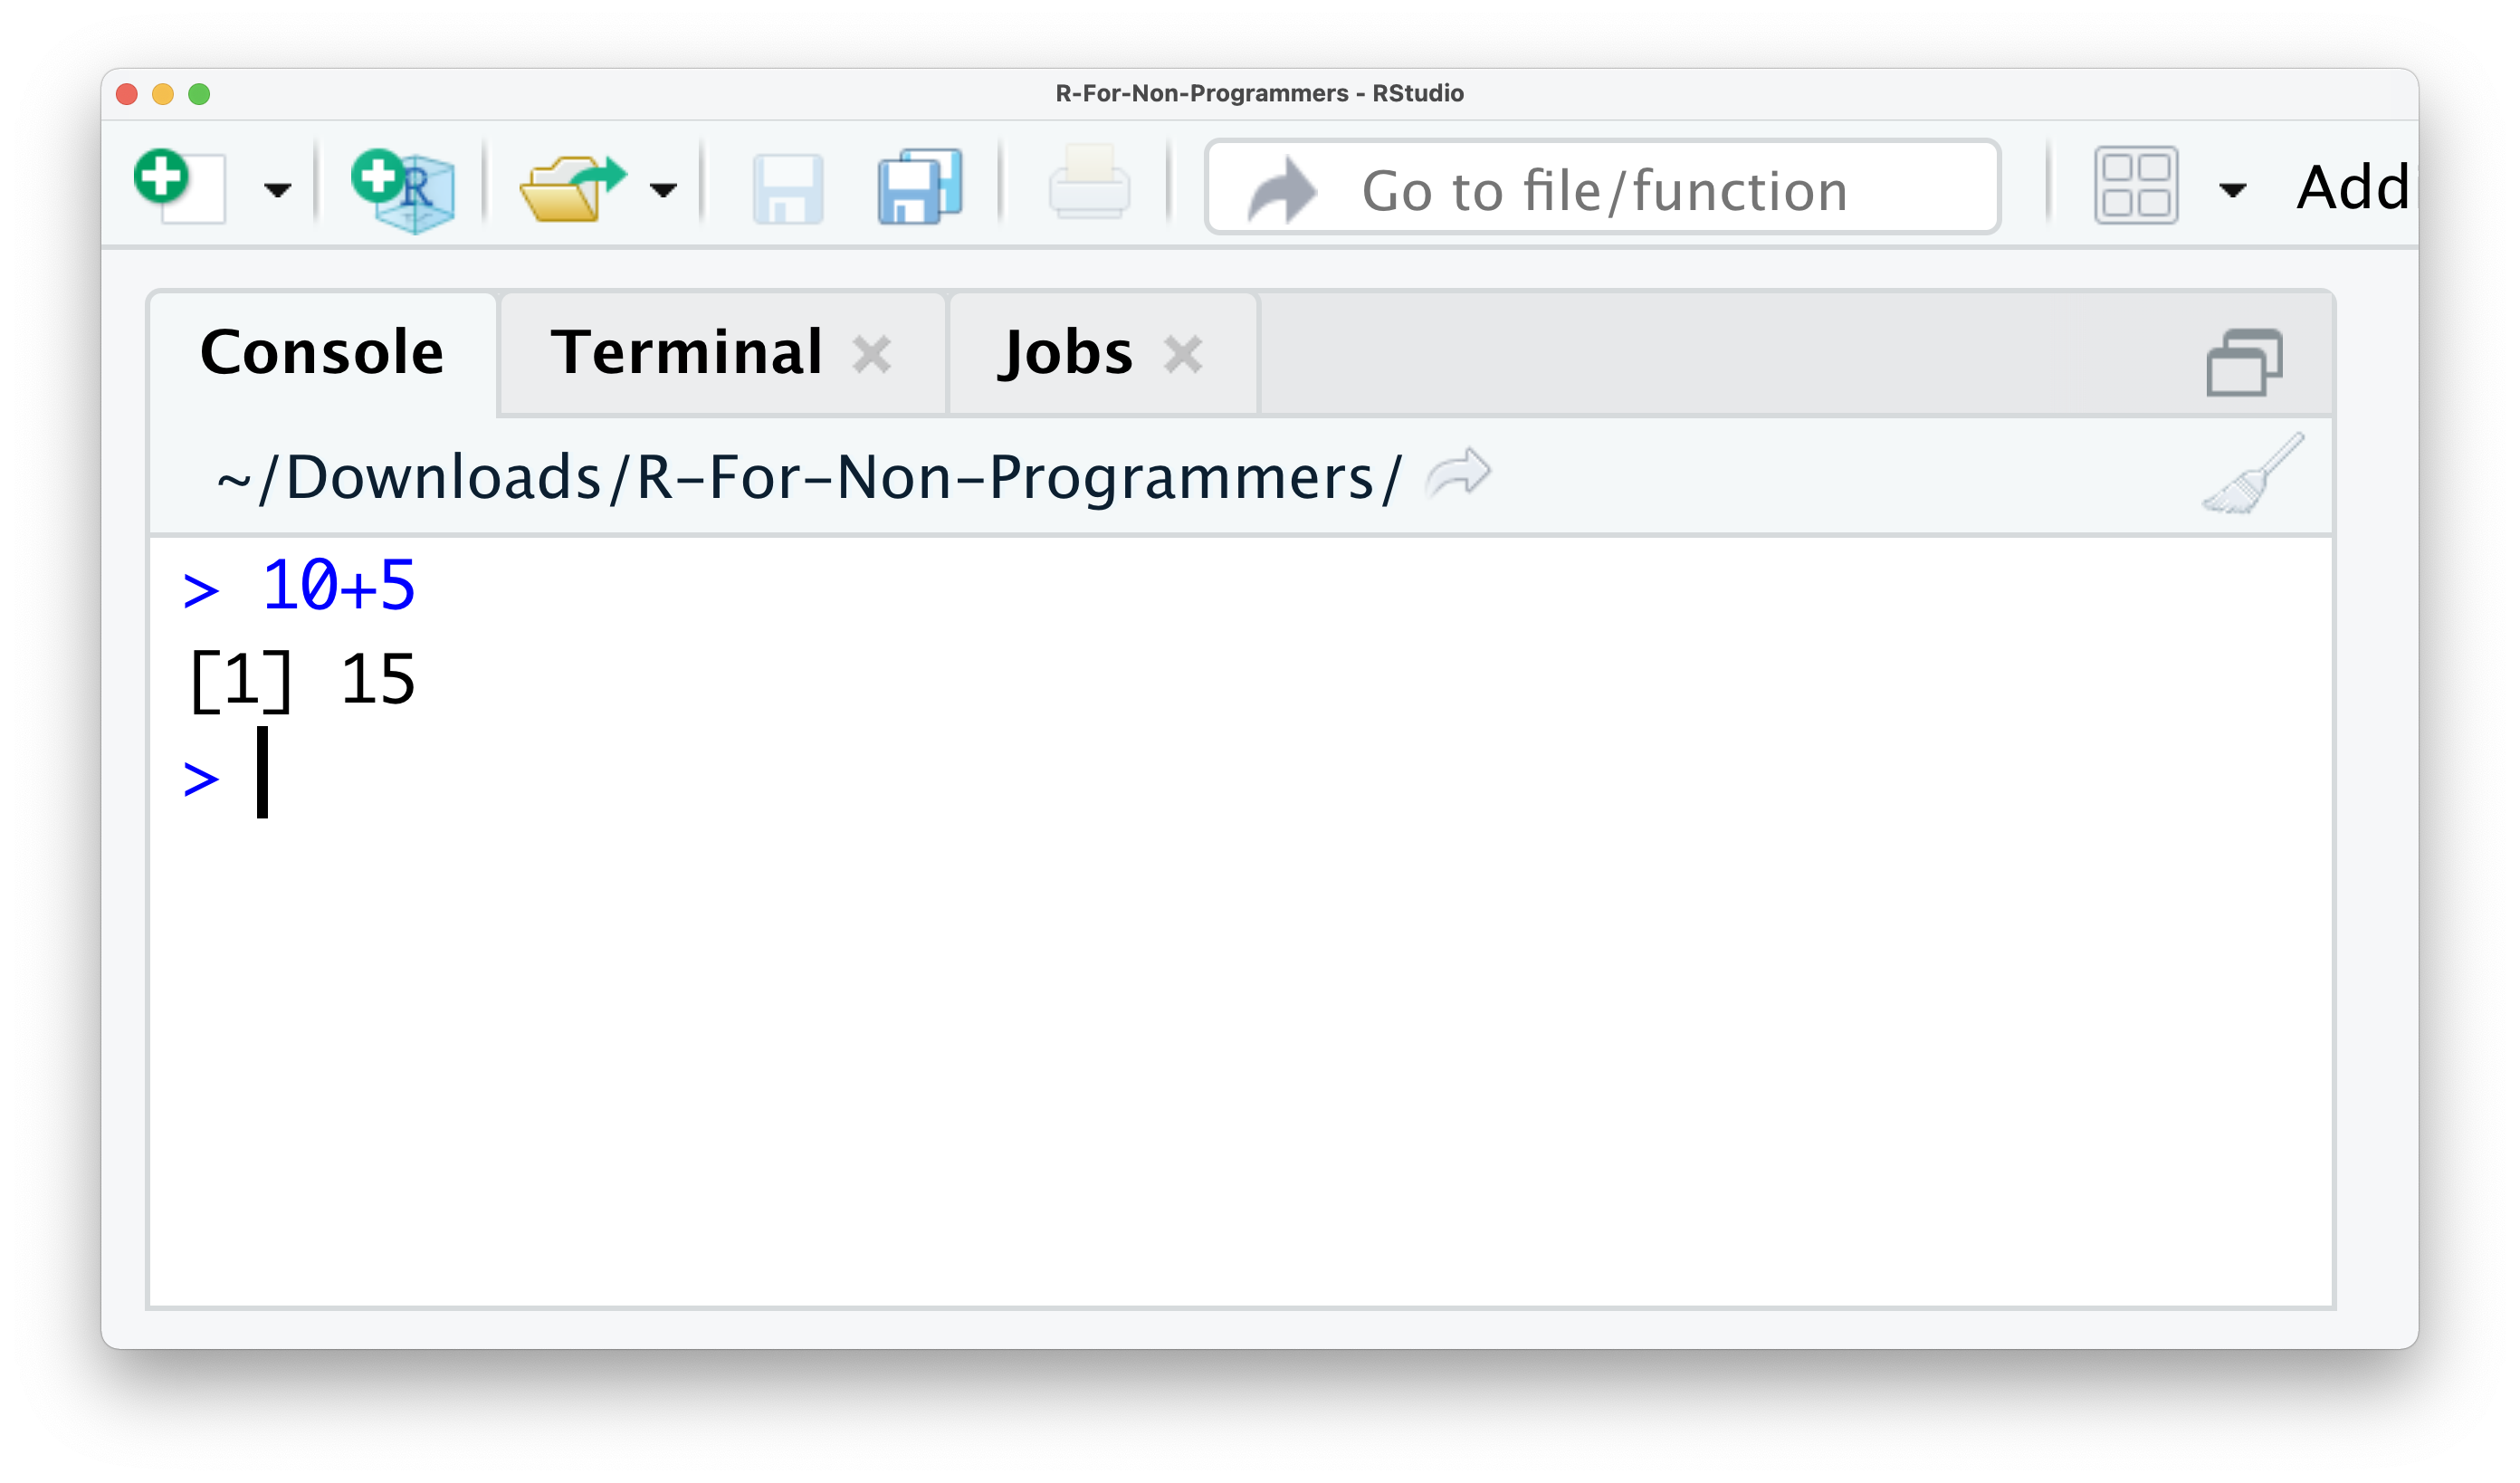
\includegraphics{images/chapter_04_img/02_console_window/console_algebra.png}

You just successfully performed your first successful computation. I
know this is not quite impressive just yet. \emph{R} is undoubtedly more
than just a giant pocket calculator.

In the top right of the console, you find a symbol resembling a broom.
This one is quite important because it clears your console. Sometimes,
the console can become very cluttered and difficult to read. If you want
to remove whatever you computed, you can click the broom icon and clear
the console of all text. I use it so frequently that I strongly
recommend learning the keyboard shortcut, which is \texttt{Ctrl\ +\ L}
on PC and Mac.

\section{The Source window}\label{sec-the-source-window}

In the top left, you can find the source window. The term `source' can
be understood as any type of file, e.g.~data, programming code, notes,
etc. The source panel can fulfil many functions, such as:

\begin{itemize}
\item
  Inspect data in an Excel-like format (see also
  Section~\ref{sec-import-your-data})
\item
  Open programming code, e.g.~an \emph{R} Script (see
  Section~\ref{sec-creating-an-r-script})
\item
  Open other text-based file formats, e.g.

  \begin{itemize}
  \item
    Plain text (.txt),
  \item
    Markdown (.md),
  \item
    Websites (.html),
  \item
    LaTeX (.tex),
  \item
    BibTex (.bib),
  \end{itemize}
\item
  Edit scripts with code in it,
\item
  Run the analysis you have written.
\end{itemize}

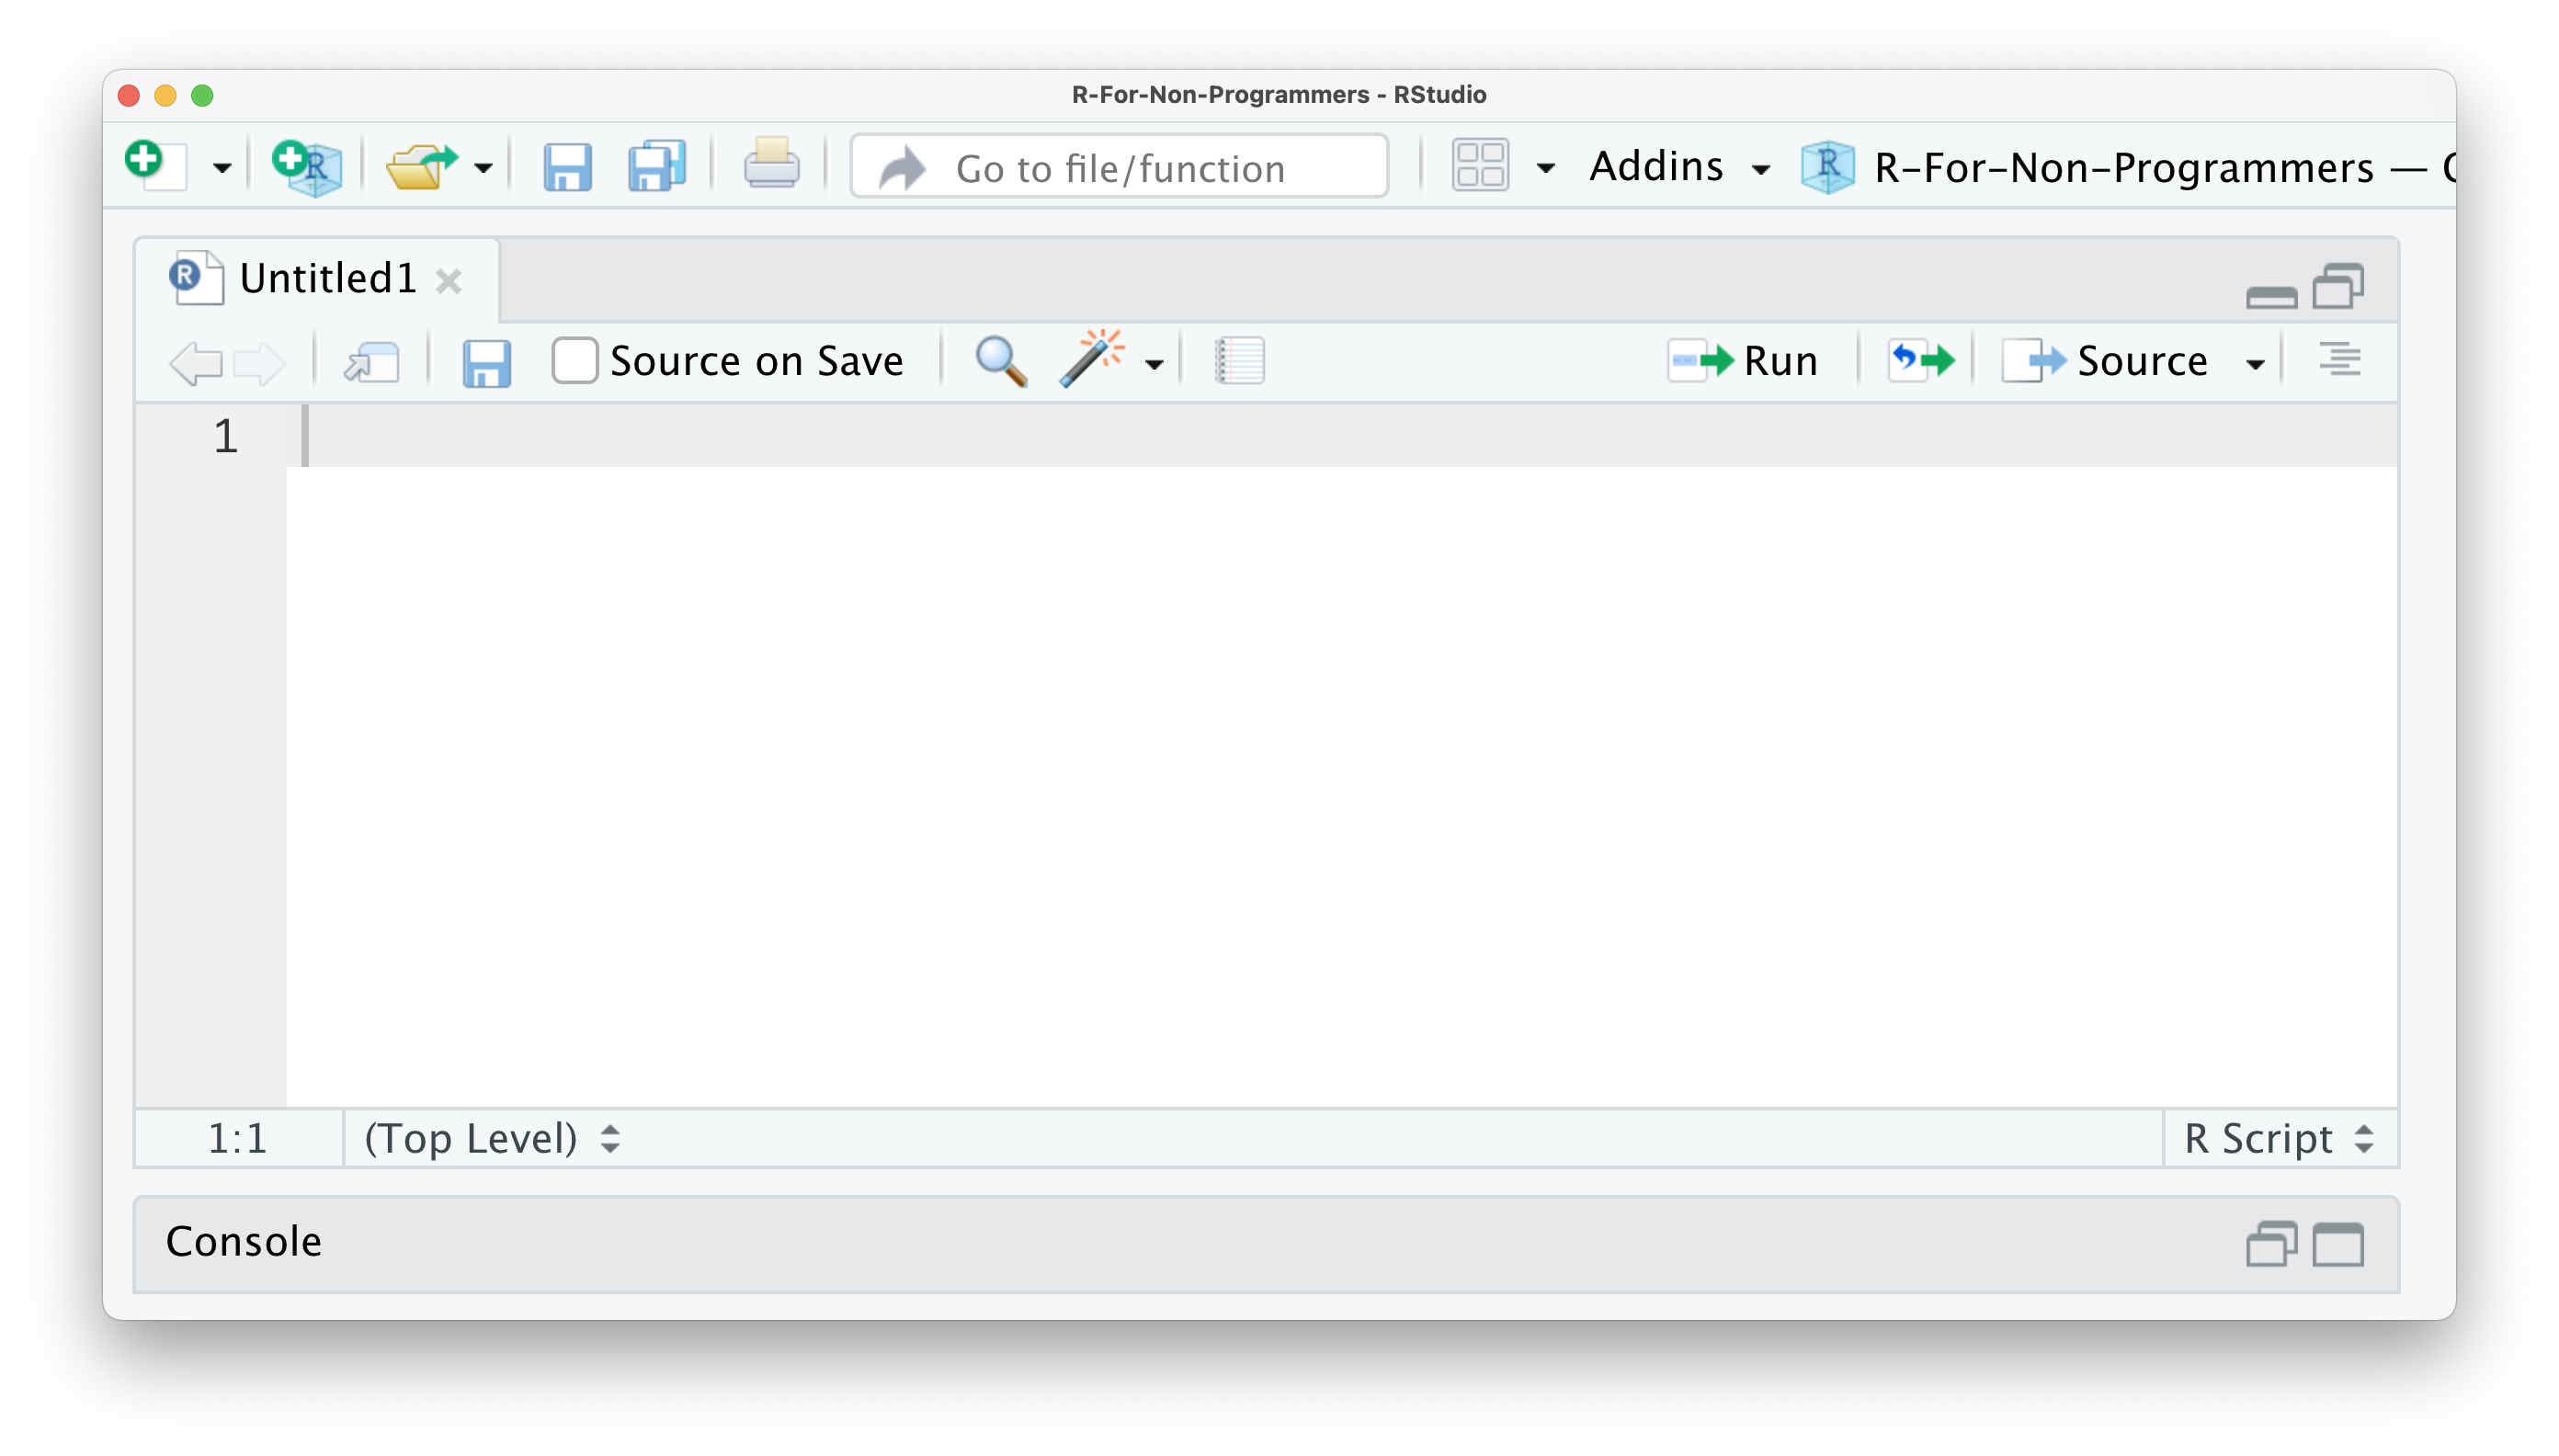
\includegraphics{images/chapter_04_img/03_source_window/01_rstudio_source.png}

In other words, the source window will show you whatever file you are
interested in, as long as RStudio can read it - and no, Microsoft Office
Documents are not supported. Another limitation of the source window is
that it can only show text-based files. So, opening images, etc. would
not work.

\section{The Environment / History / Connections / Tutorial
window}\label{sec-the-environment-history-connections-tutorial-window}

The window in the top right shows multiple panes. The first pane is
called \emph{Environment} and shows you objects available for
computation. One of the first objects you will create is your dataset
because, without data, we cannot perform any analysis. Another object
could be a plot showing the number of male and female participants in
your study. To find out how to create objects yourself, you can take a
glimpse at it (see Section~\ref{sec-inspecting-raw-data}). Besides
datasets and plots, you will also find other objects here, e.g.~lists,
vectors and functions you created yourself. Don't worry if none of these
words makes sense at this point. We will cover each of them in the
upcoming chapters. For now, remember this is a place where you can find
different objects you created and might need for your analysis.

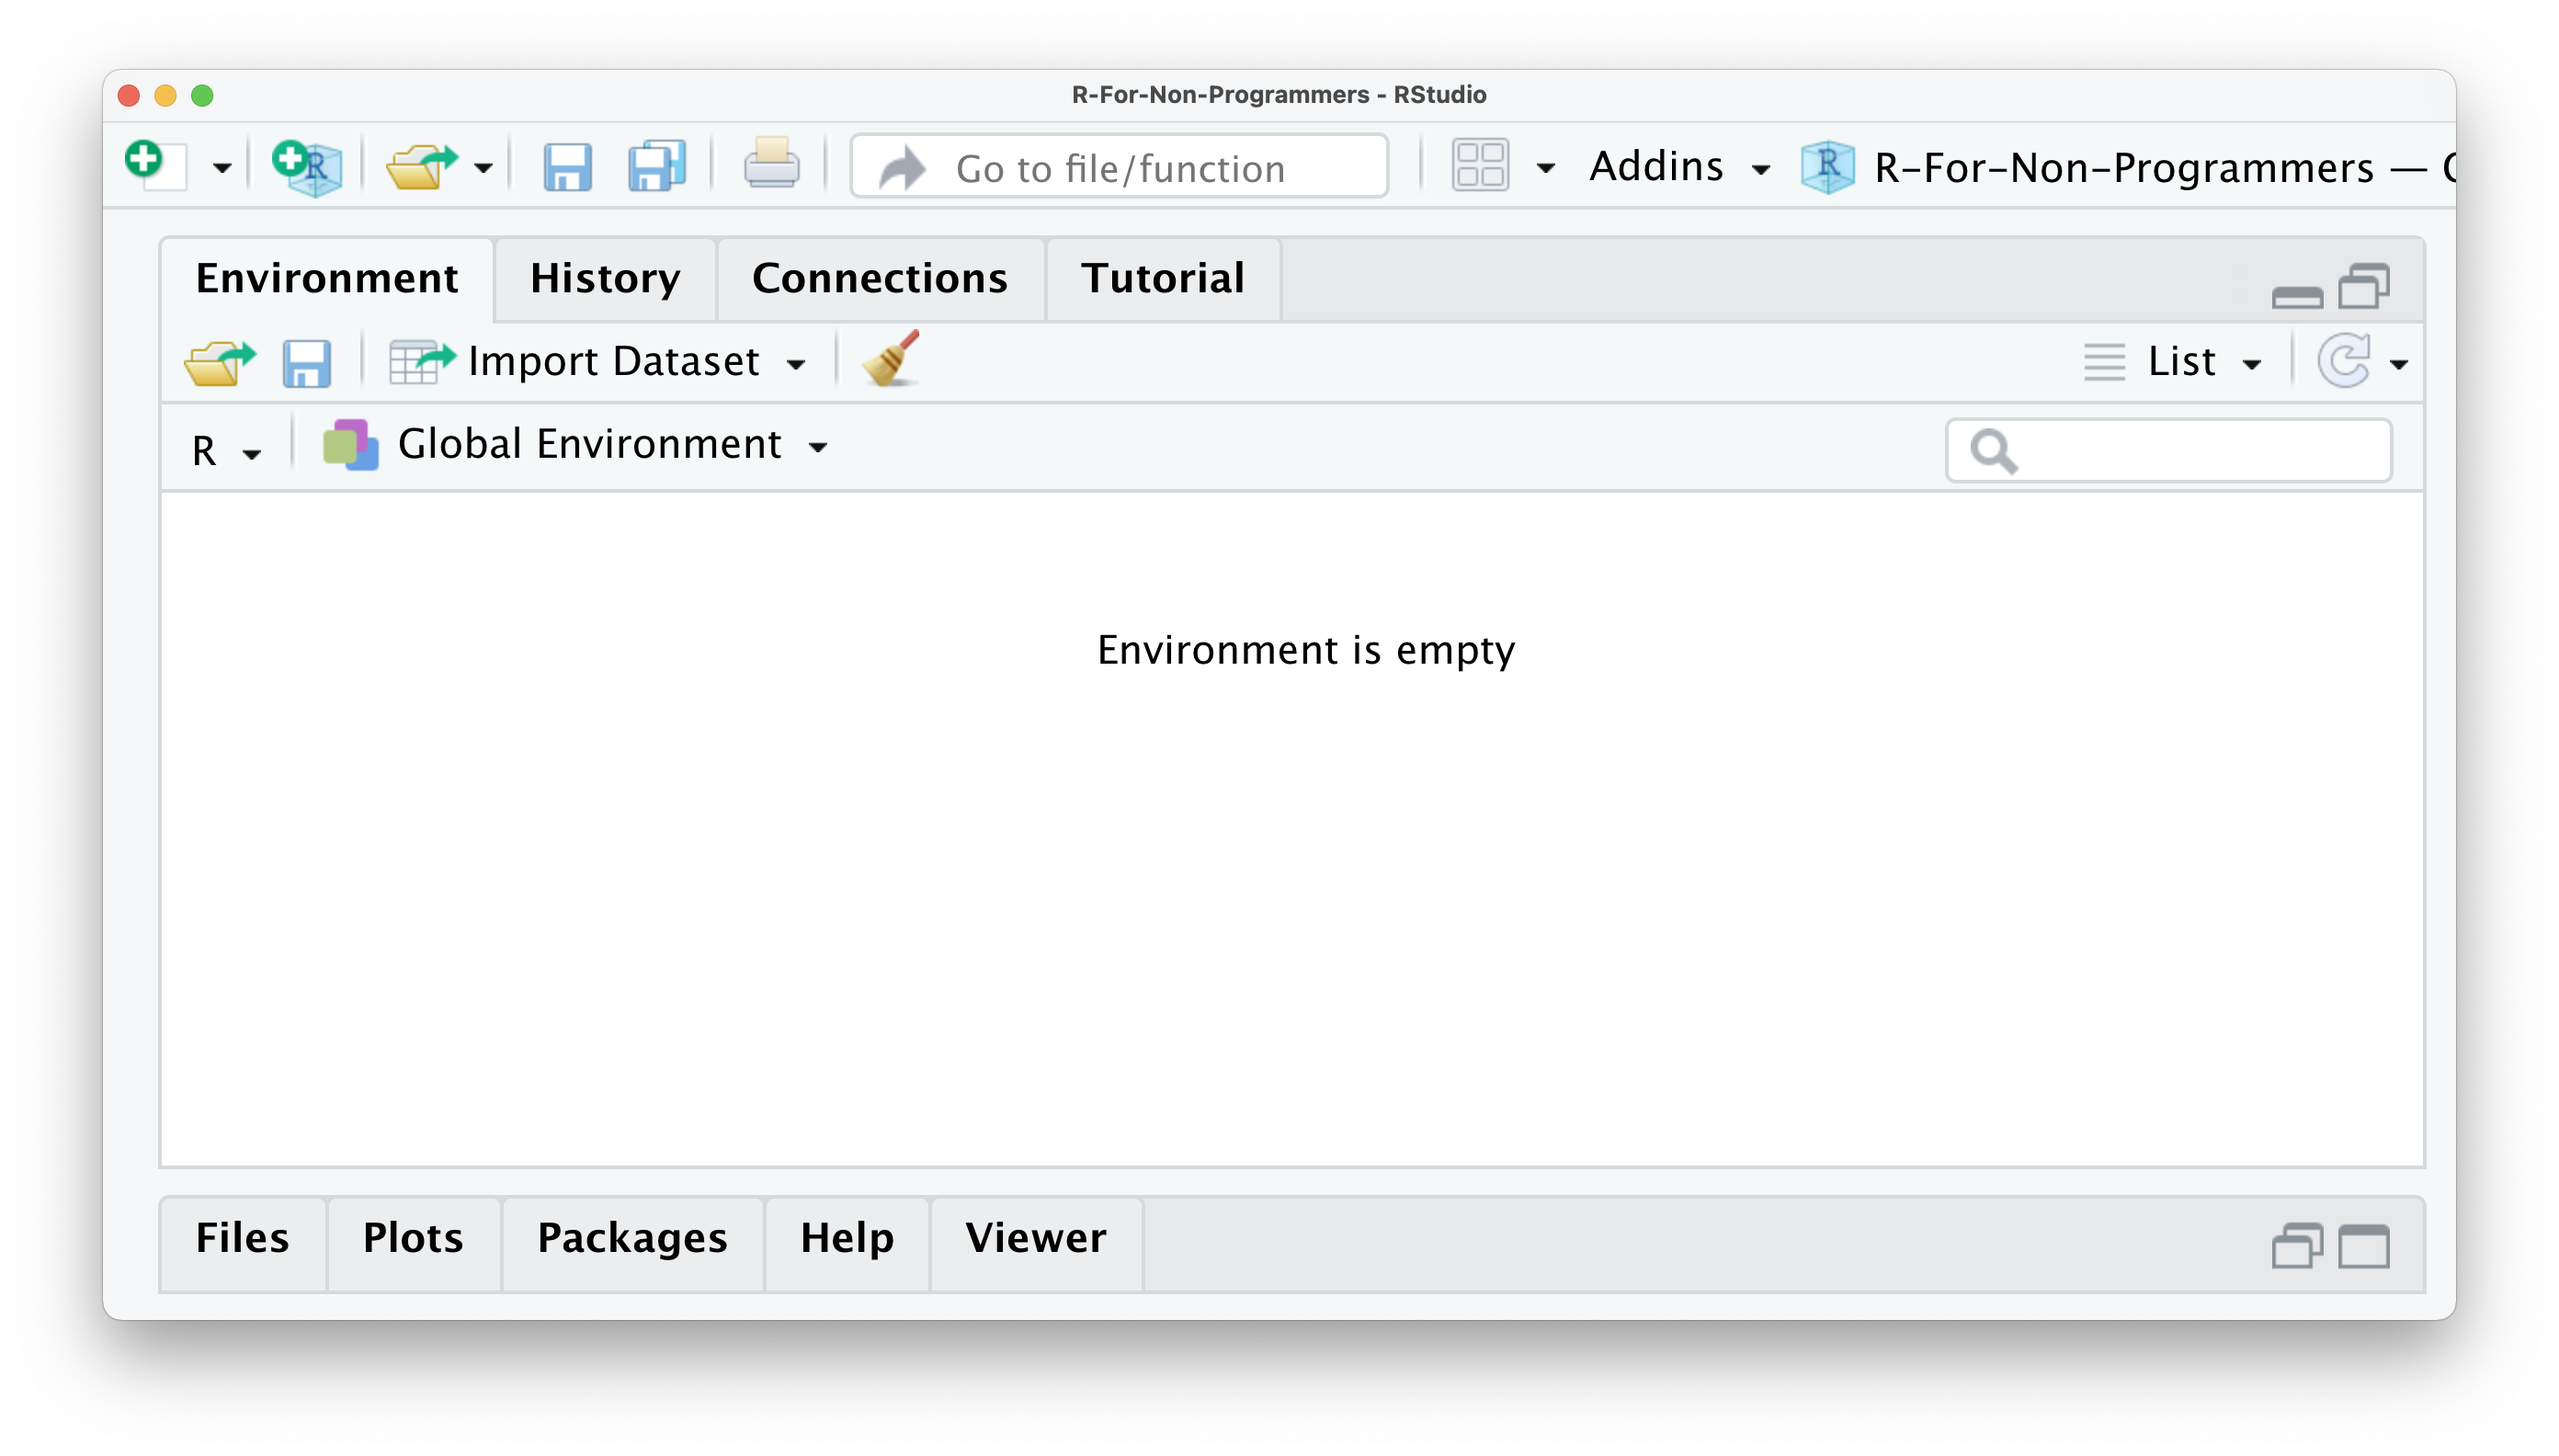
\includegraphics{images/chapter_04_img/04_environment_history_etc/01_rstudio_environment.png}

The \emph{History} pane is very easy to understand. Whatever computation
you run in the console will be stored. So you can go back and see what
you coded and rerun that code. Remember the example from above where we
computed the sum of \texttt{10+5}? This computation is stored in the
history of RStudio, and you can rerun it by clicking on \texttt{10+5} in
the history pane and then clicking on \texttt{To\ Console}. This will
insert \texttt{10+5} back into the console, and we can hit
\texttt{Return} to retrieve the result. You also have the option to copy
the code into an existing or new \emph{R} Script by clicking on
\texttt{To\ Source}. By doing this, you can save this computation on
your computer and reuse it later. Finally, if you would like to store
your history, you can do so by clicking on the
\texttt{floppy\ disk\ symbol}. There are two more buttons in this pane,
one allows you to delete individual entries in the history (the white
page with the red circle on it), and the last one, a \texttt{broom},
clears the entire history (irrevocably).

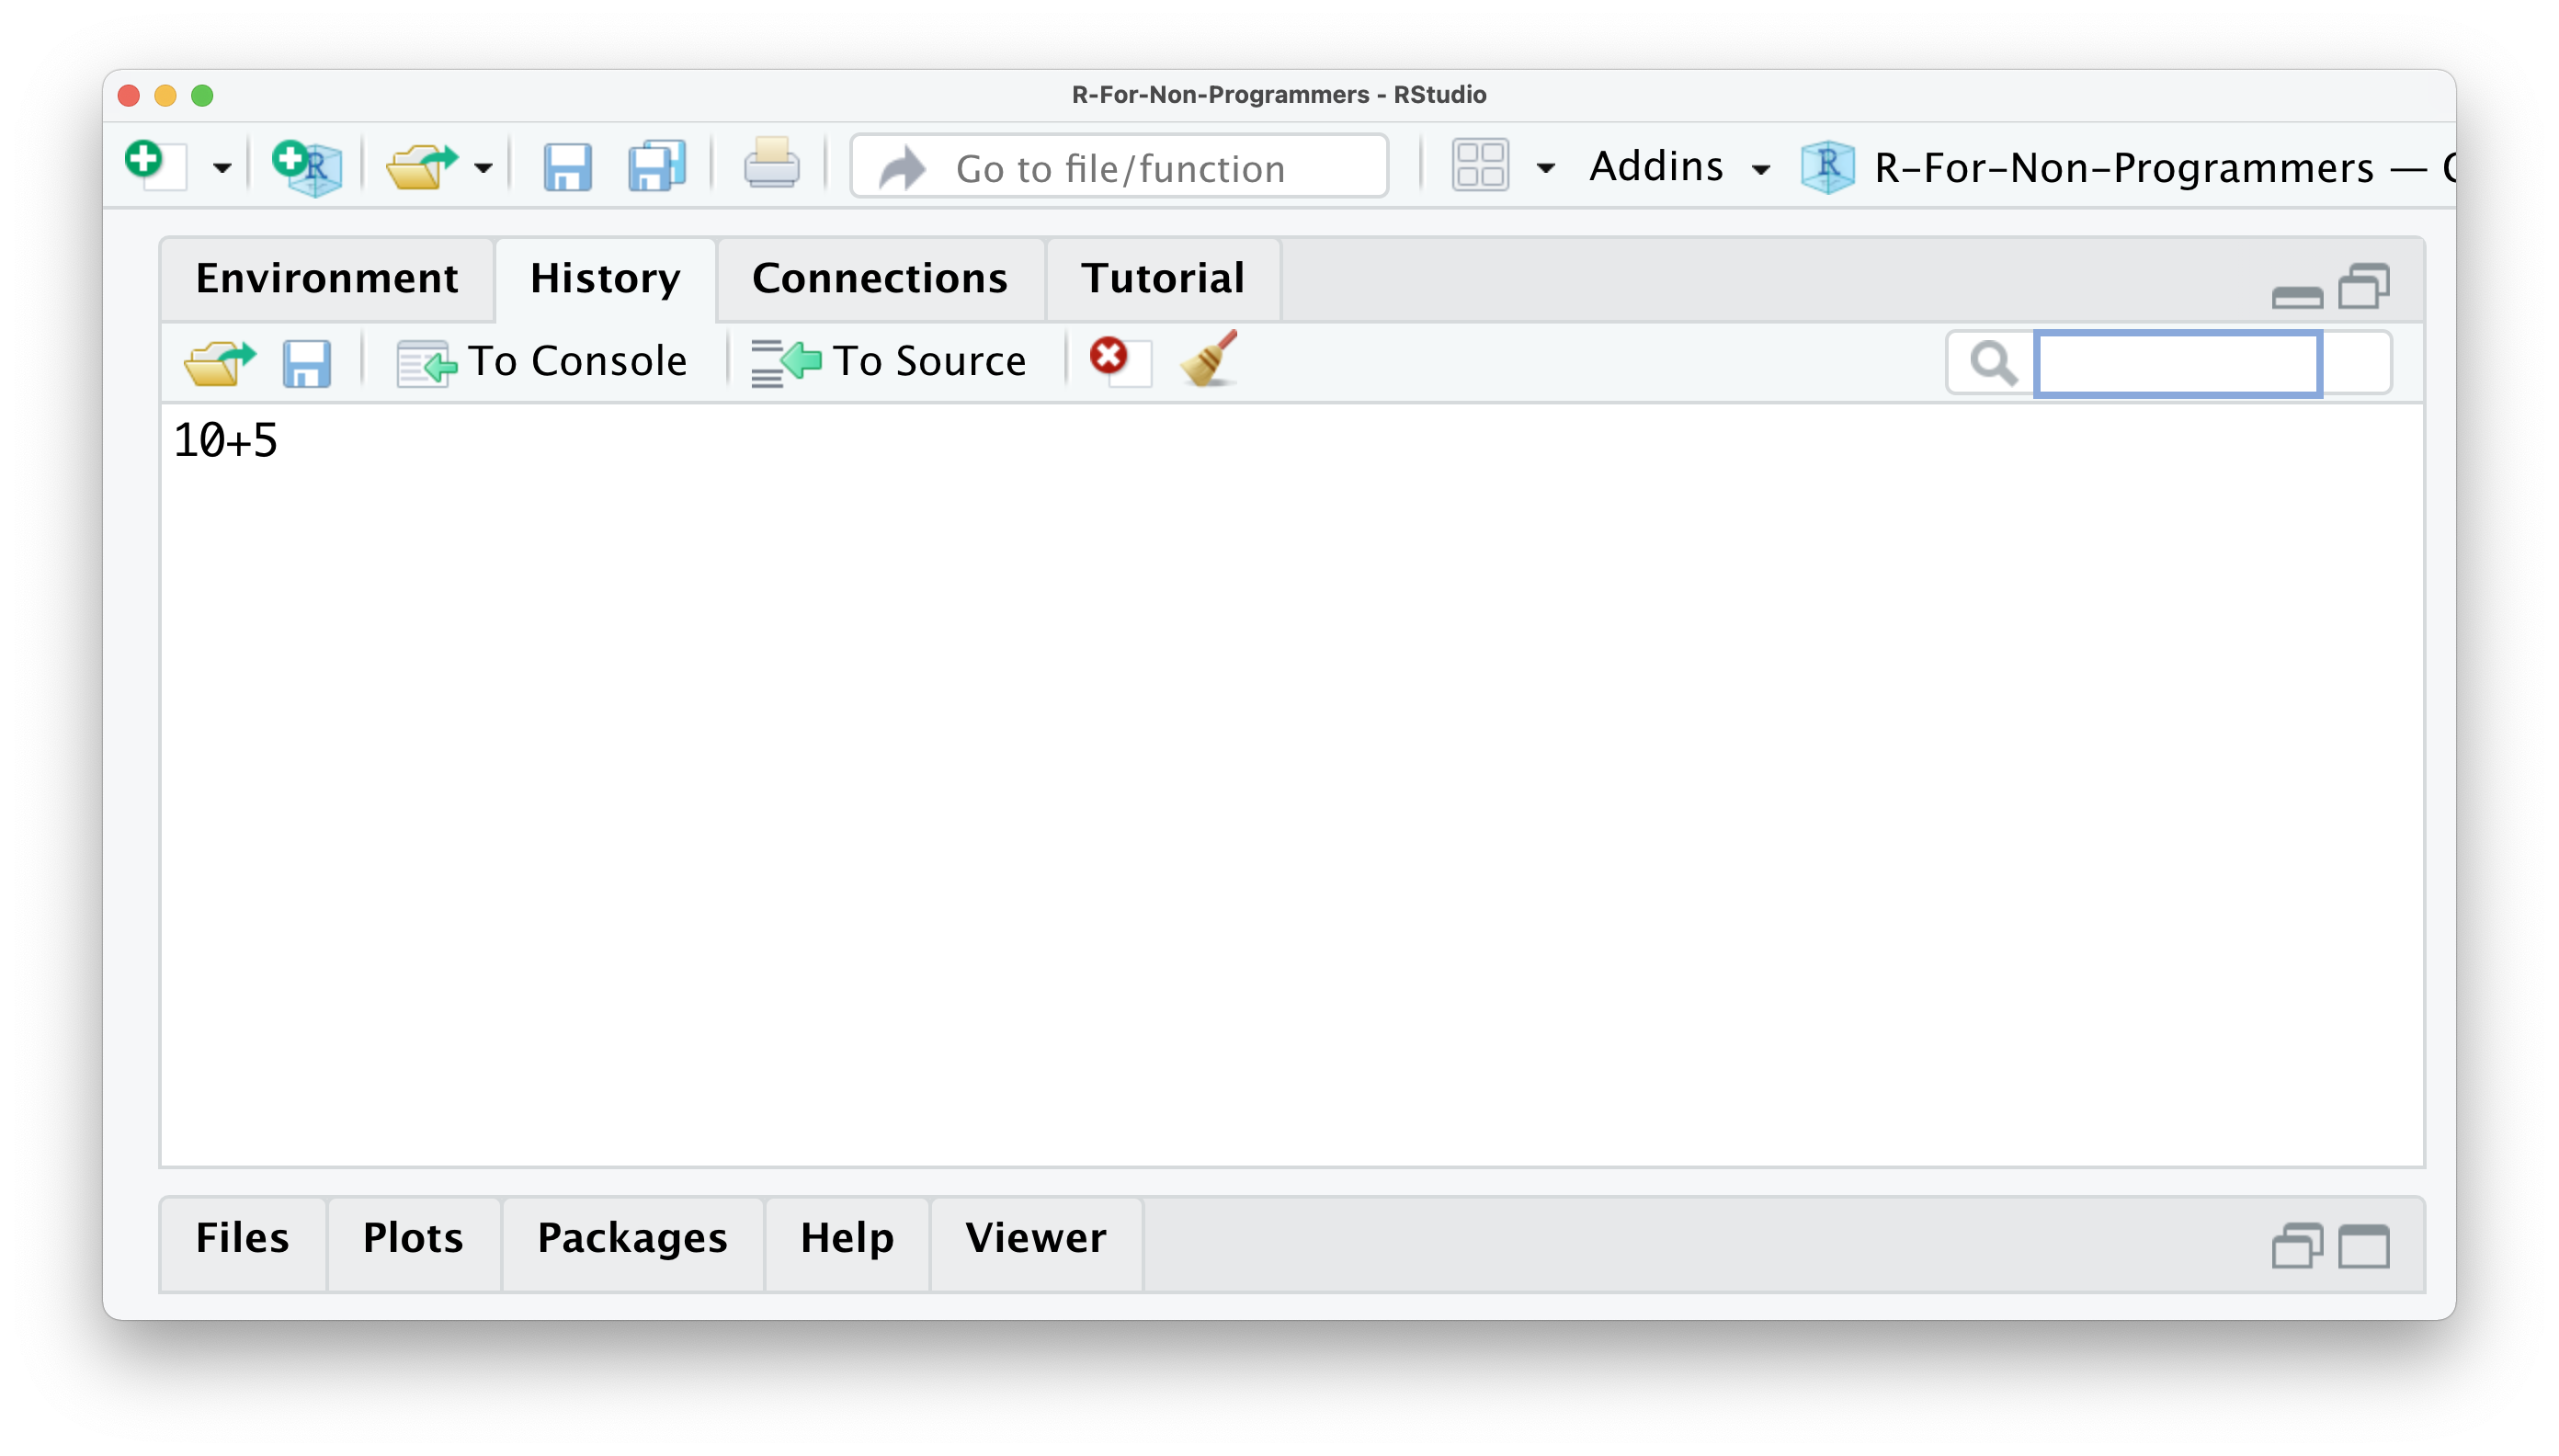
\includegraphics{images/chapter_04_img/04_environment_history_etc/02_rstudio_history.png}

The pane \emph{Connections} allows you to tap into external databases
directly. This can come in handy when you work collaboratively on the
same data or want to work with extensive datasets without downloading
them. However, for an introduction to \emph{R}, we will not use this
feature of RStudio.

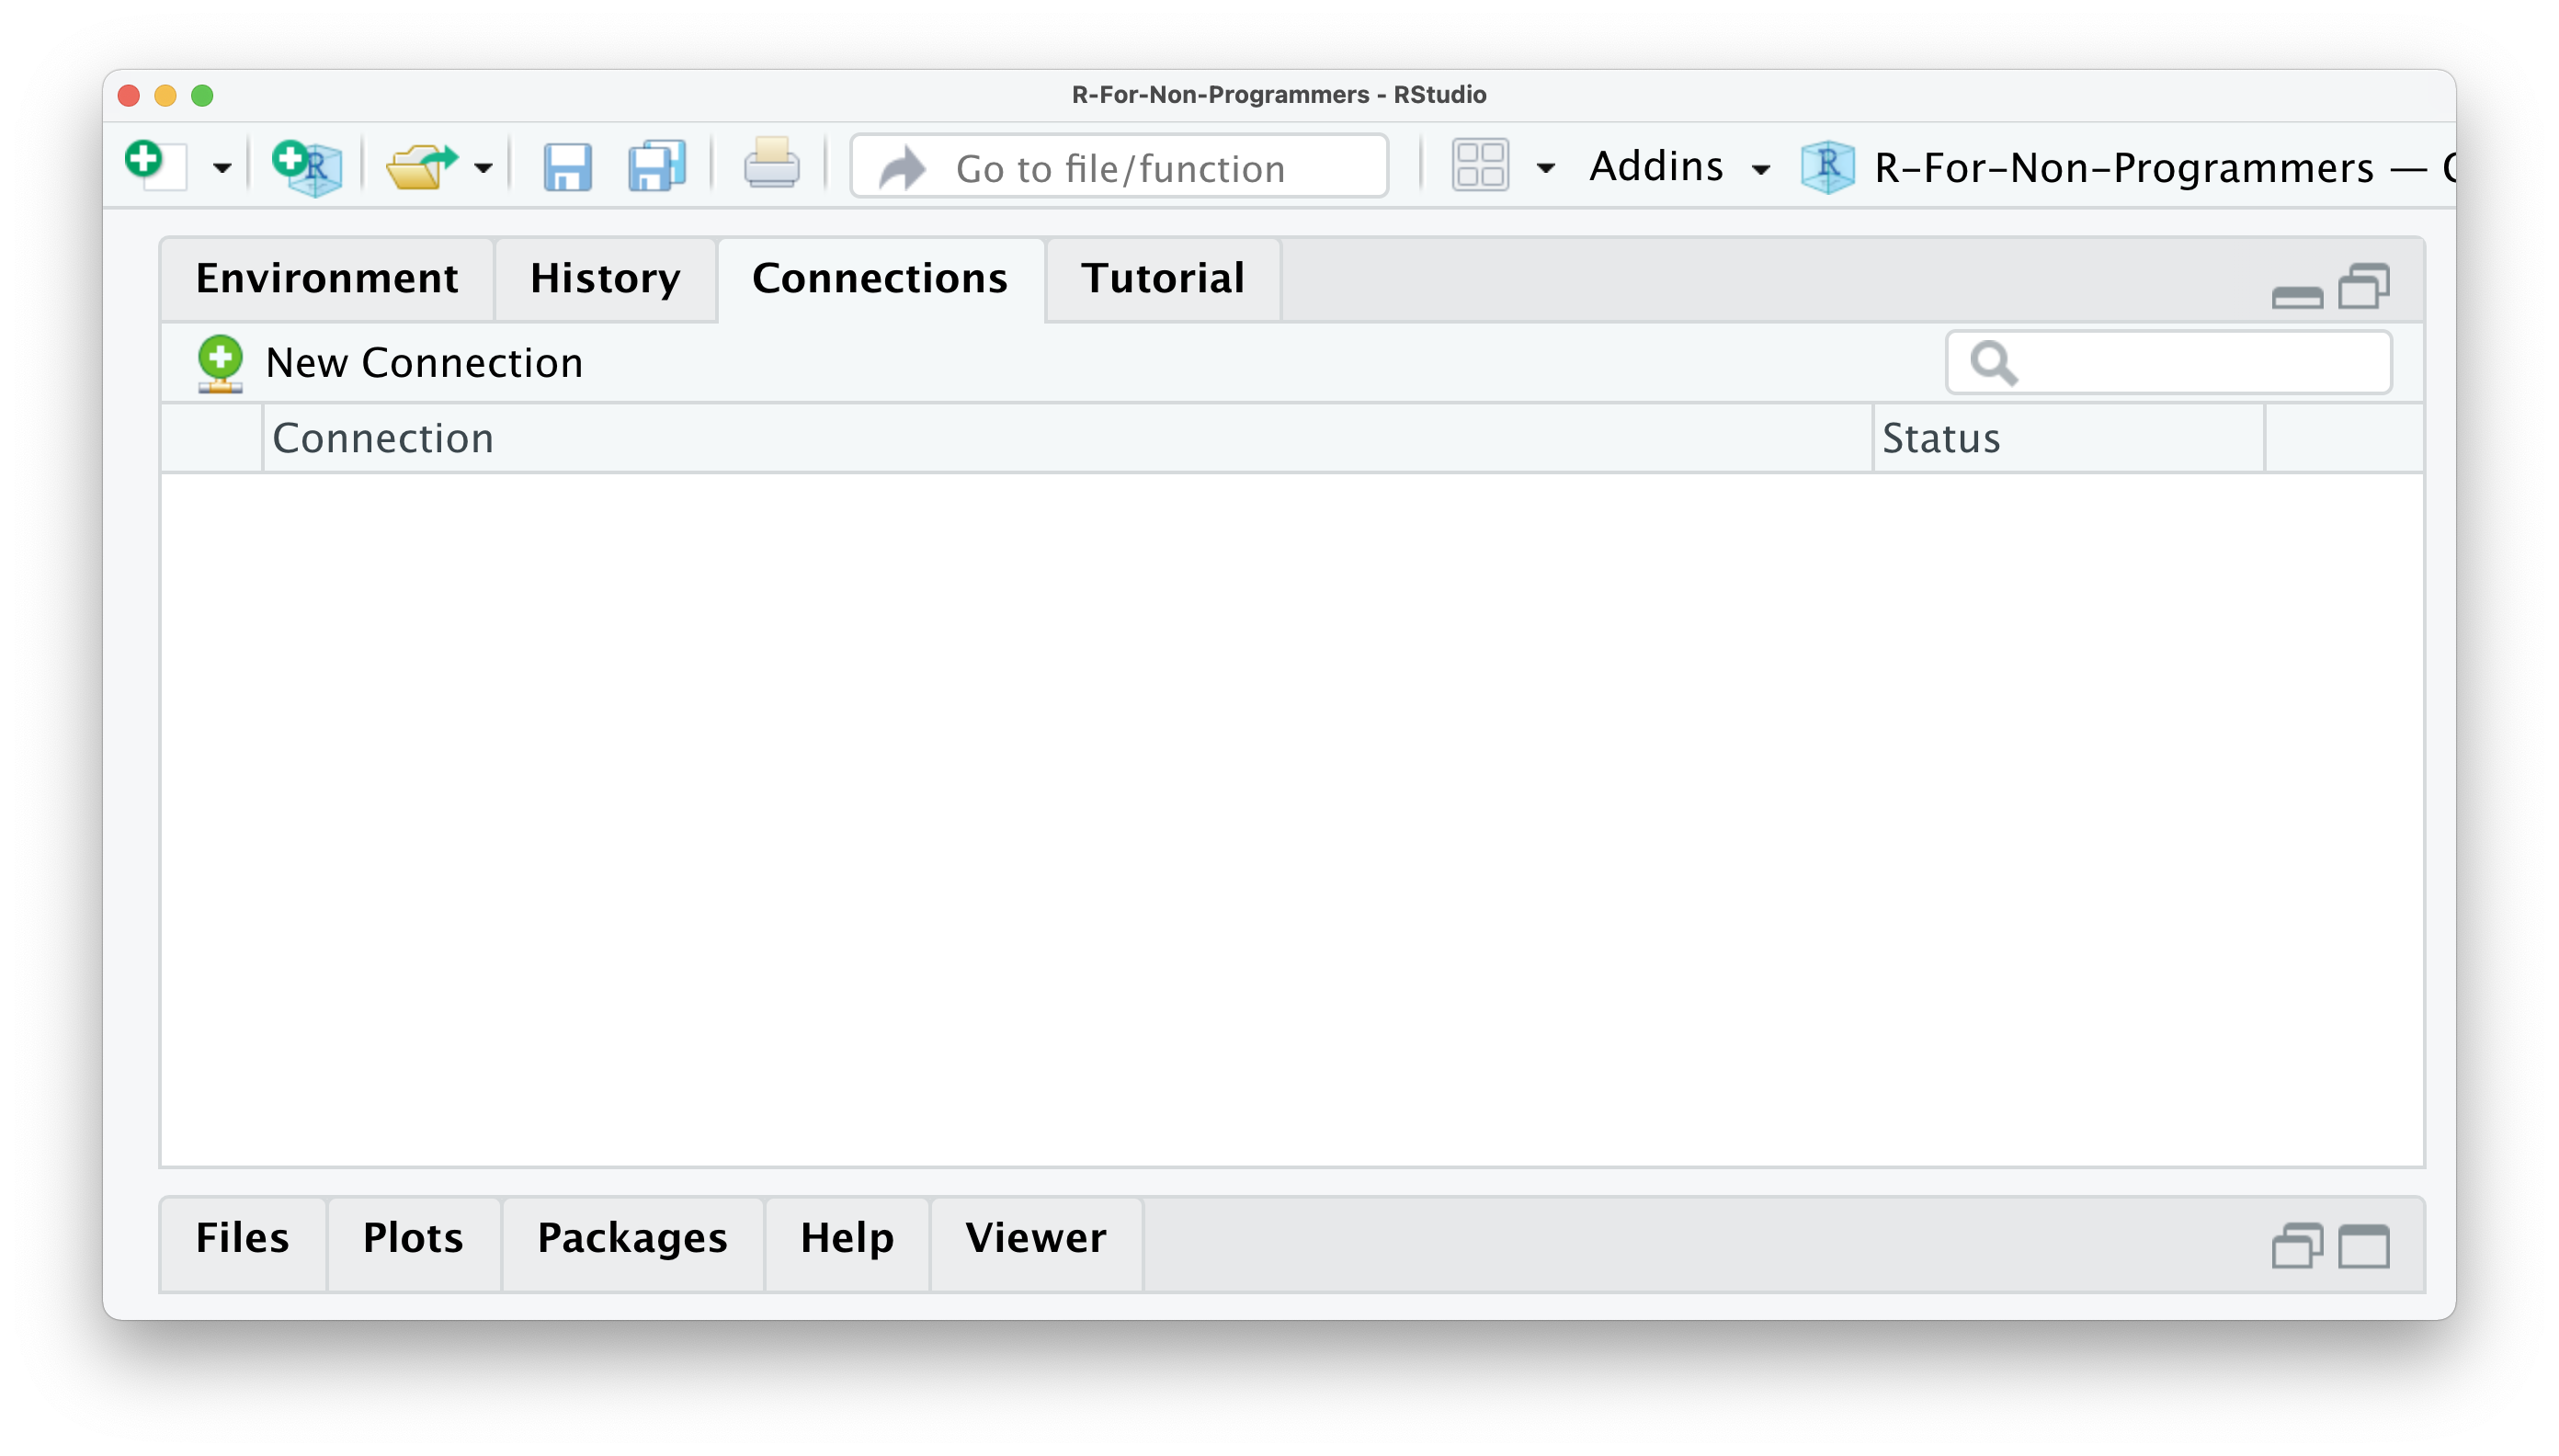
\includegraphics{images/chapter_04_img/04_environment_history_etc/03_rstudio_connections.png}

The last pane is called \emph{Tutorial}. Here, you can find additional
materials on learning \emph{R} and RStudio. If you search for more great
content to learn \emph{R}, this sis an excellent starting point.

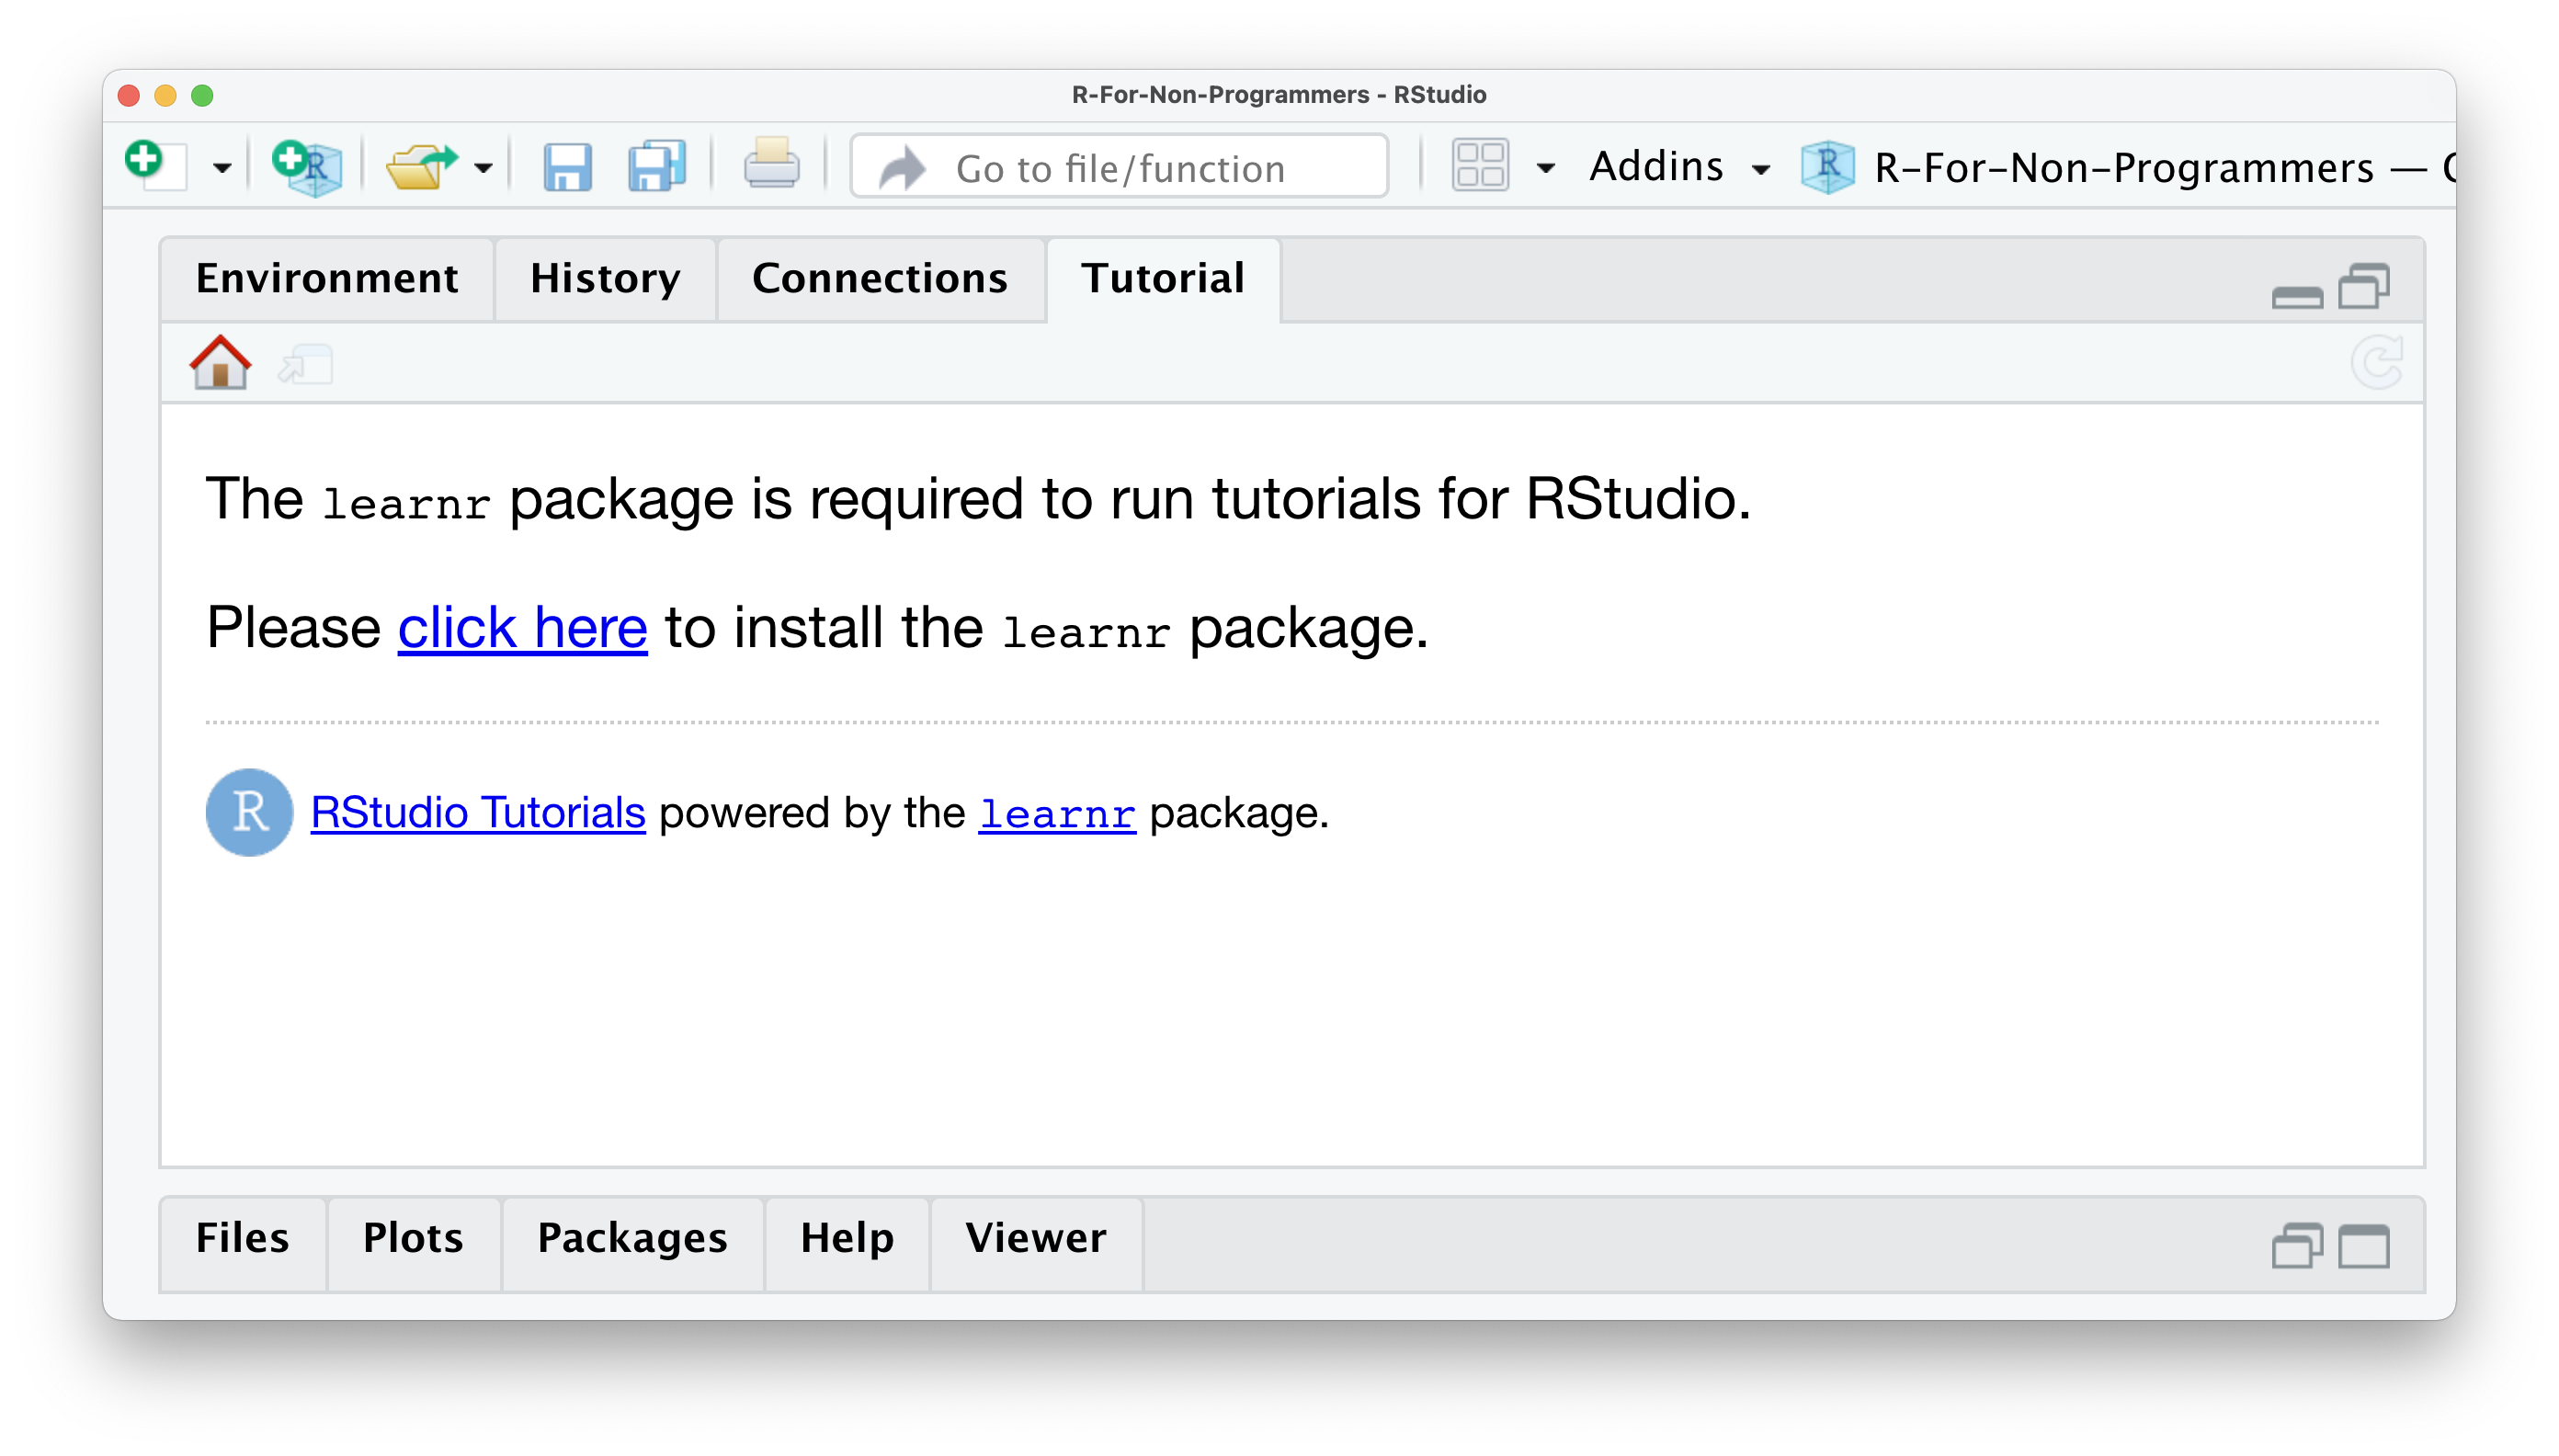
\includegraphics{images/chapter_04_img/04_environment_history_etc/04_rstudio_tutorial.png}

\section{The Files / Plots / Packages / Help / Viewer
window}\label{sec-the-files-plots-packages-help-viewer-window}

The last window consists of five essential panes. The first one is the
\emph{Files} pane. As the name indicates, it lists all the files and
folders in your root directory. A root directory is the default
directory where RStudio saves your files, for example, your analysis.
However, we will look at how you can properly set up your projects in
RStudio in Chapter~\ref{sec-starting-your-r-projects}. Thus, the
\emph{Files} pane is an easy way to load data into RStudio and create
folders to keep your research project well organised.

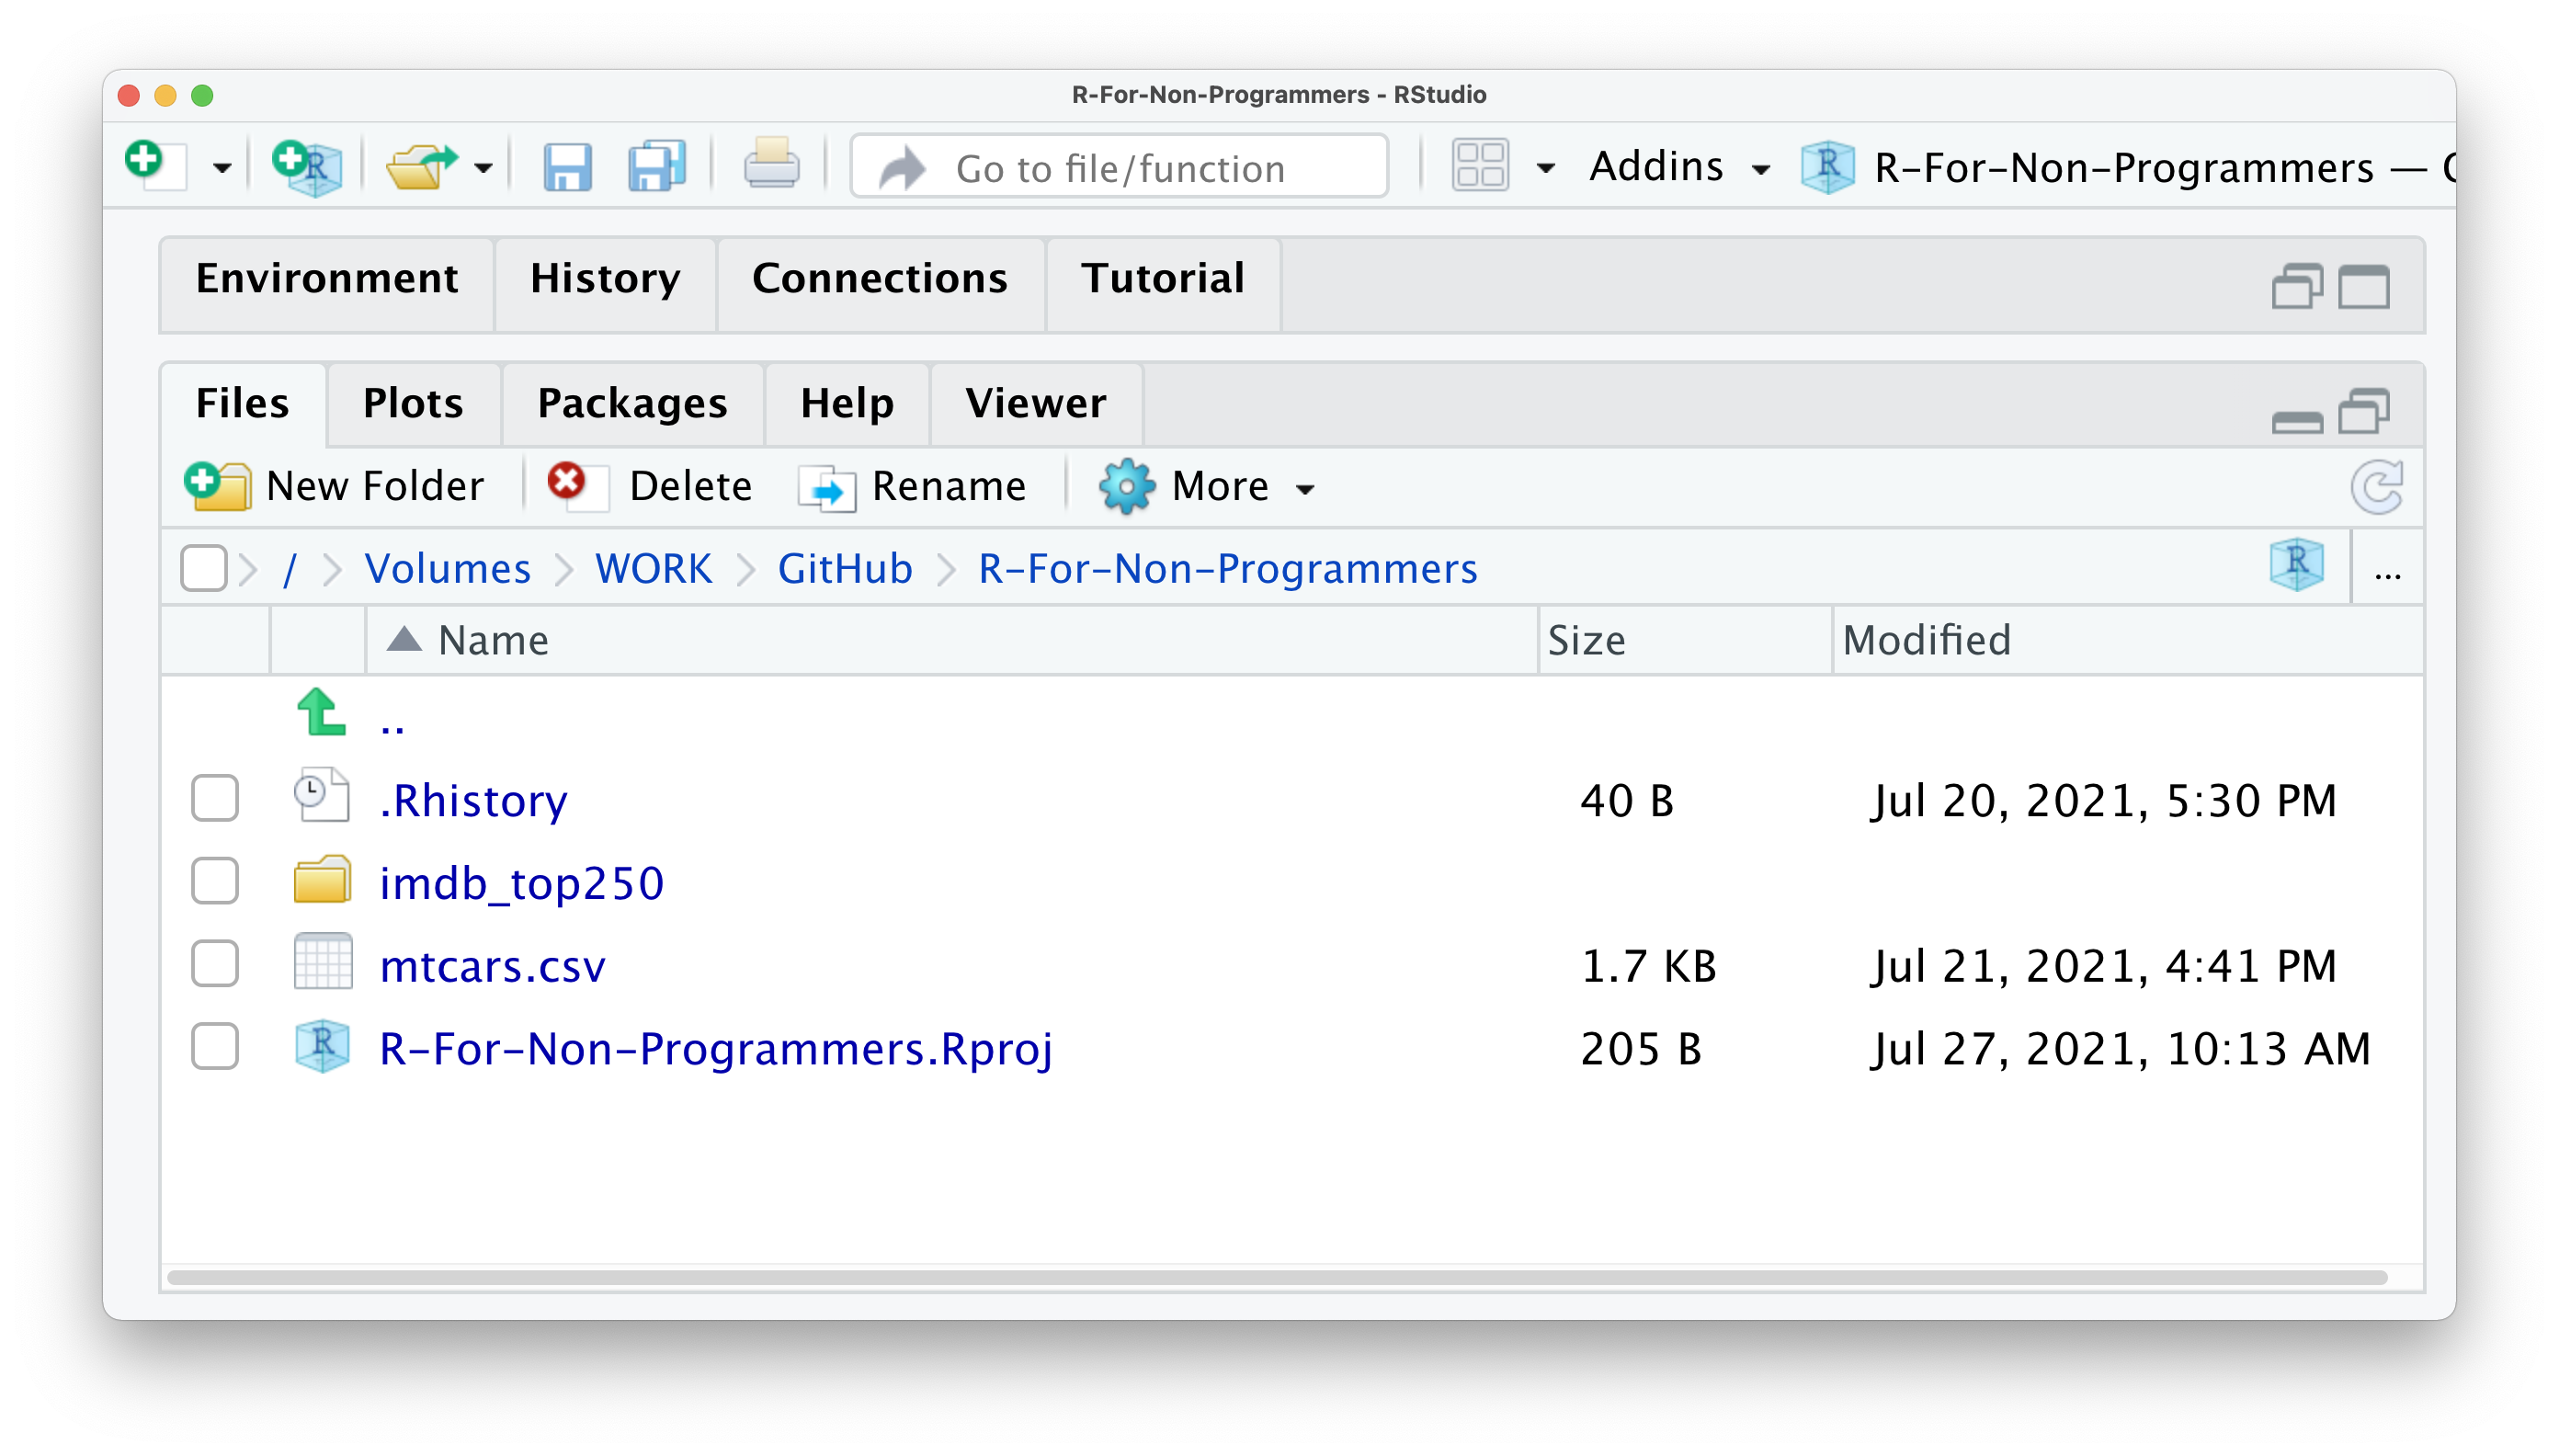
\includegraphics{images/chapter_04_img/05_files_plots_etc/01_rstudio_files.png}

Since the Console cannot reproduce data visualisations, RStudio offers a
way to do this very easily. It is through the \emph{Plots} pane. This
pane is exclusively designed to show you any plots you have created
using \emph{R}. Here is a simple example that you can try. Type into
your console \texttt{boxplot(mtcars\$hp)}.

\begin{Shaded}
\begin{Highlighting}[]
\CommentTok{\# Here we create a nice boxplot using a dataset called \textquotesingle{}mtcars\textquotesingle{}}
\FunctionTok{boxplot}\NormalTok{(mtcars}\SpecialCharTok{$}\NormalTok{hp)}
\end{Highlighting}
\end{Shaded}

\begin{figure}

\centering{

\captionsetup{labelsep=none}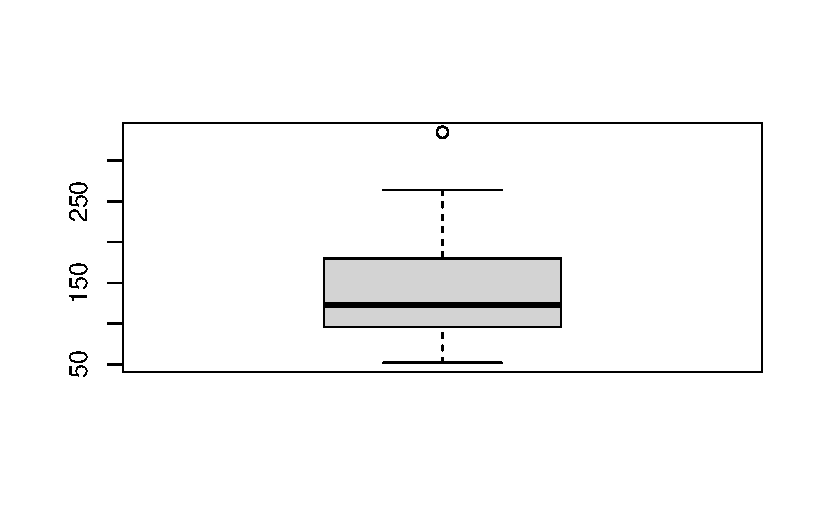
\includegraphics{04_rstudio_interface_files/figure-latex/fig-simple-boxplot-1.pdf}

}

\caption{\label{fig-simple-boxplot}}

\end{figure}%

Although this is a short piece of coding, it performs quite a lot of
steps:

\begin{itemize}
\item
  it uses a function called \texttt{boxplot()} to draw a boxplot of
\item
  a variable called \texttt{hp} (for horsepower), which is located in
\item
  a dataset named \texttt{mtcars},
\item
  and it renders the graph in your \emph{Plots} pane
\end{itemize}

This is how the plot should look like in your RStudio \emph{Plots} pane.

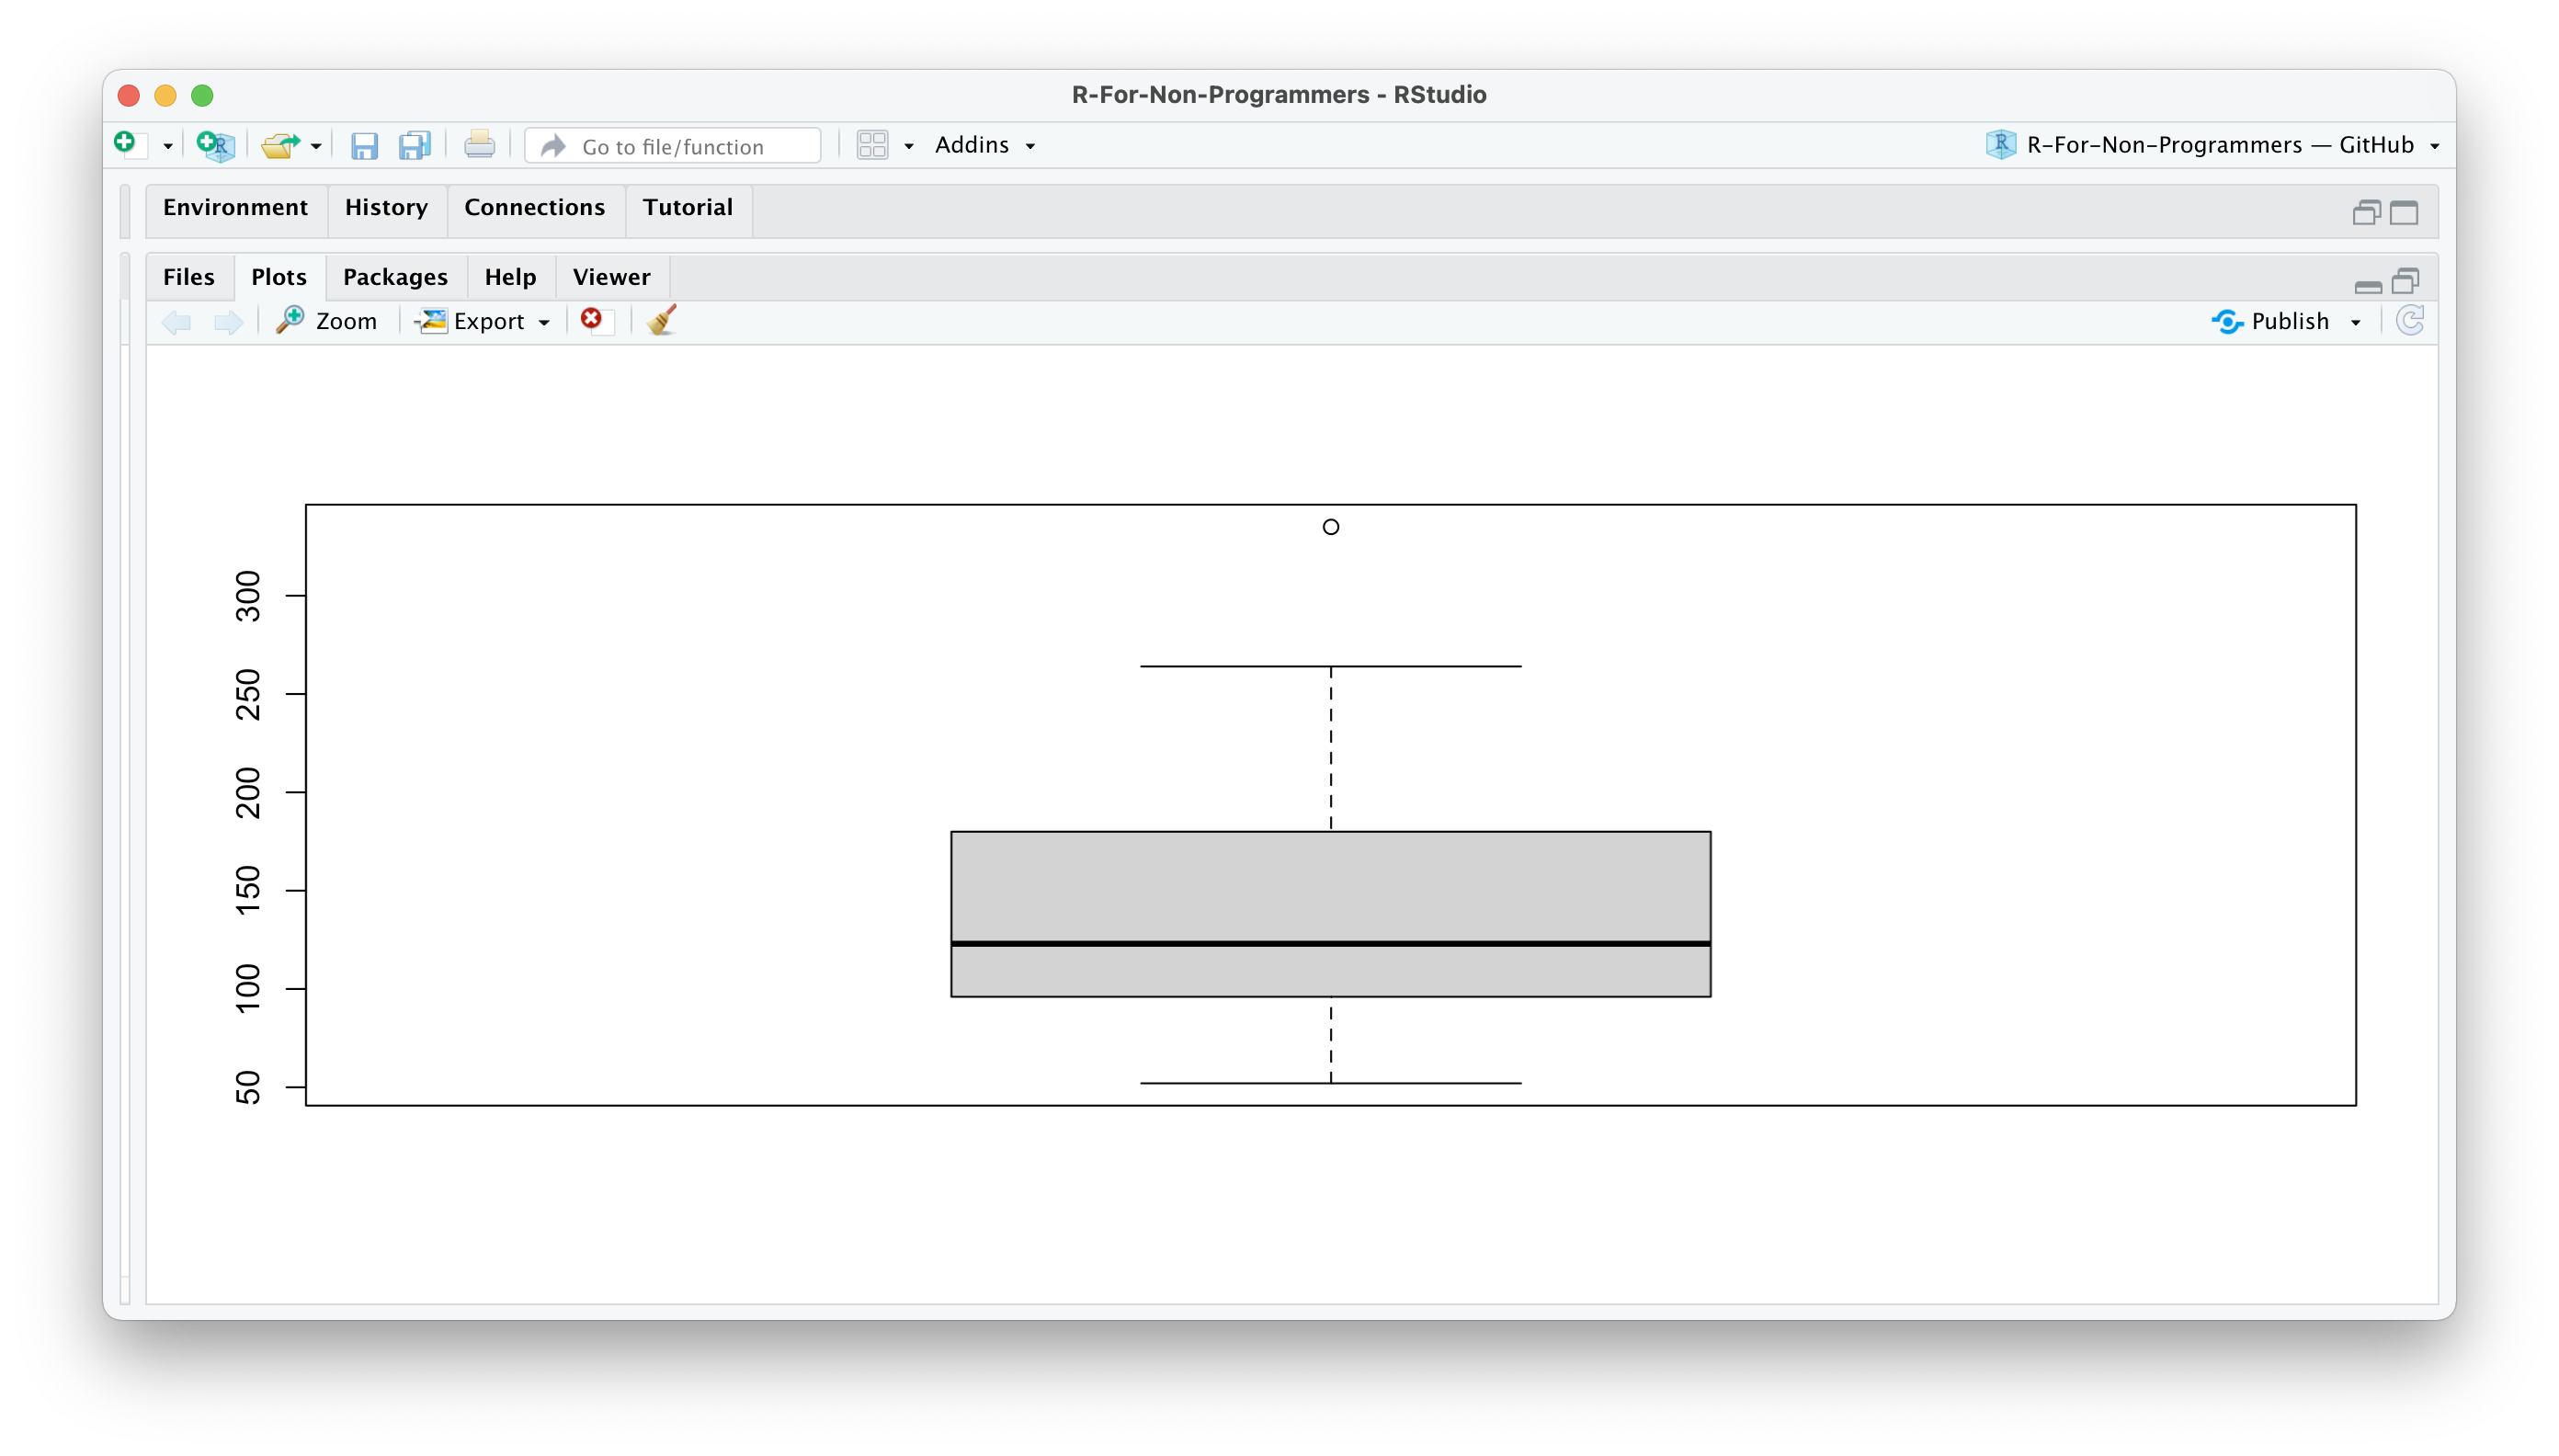
\includegraphics{images/chapter_04_img/05_files_plots_etc/02_rstudio_plots.png}

If you wish to delete the plot, you can click on the
\texttt{red\ circle\ with\ a\ white\ x} symbol. This will delete the
currently visible plot. If you wish to remove all plots from this pane,
you can use the \texttt{broom}. There is also an option to export your
plot and move back and forth between different plots.

The next pane is called \emph{Packages}. Packages are additional tools
you can import and use when performing your analysis. A frequent analogy
people use to explain packages is your phone and the apps you install.
Each package you download is equivalent to an app on your phone. It can
enhance different aspects of working in \emph{R}, such as creating
animated plots, using unique machine-learning algorithms, or simply
making your life easier by doing multiple computations with just one
single line of code. You will learn more about \emph{R packages} in
Section~\ref{sec-r-packages}.

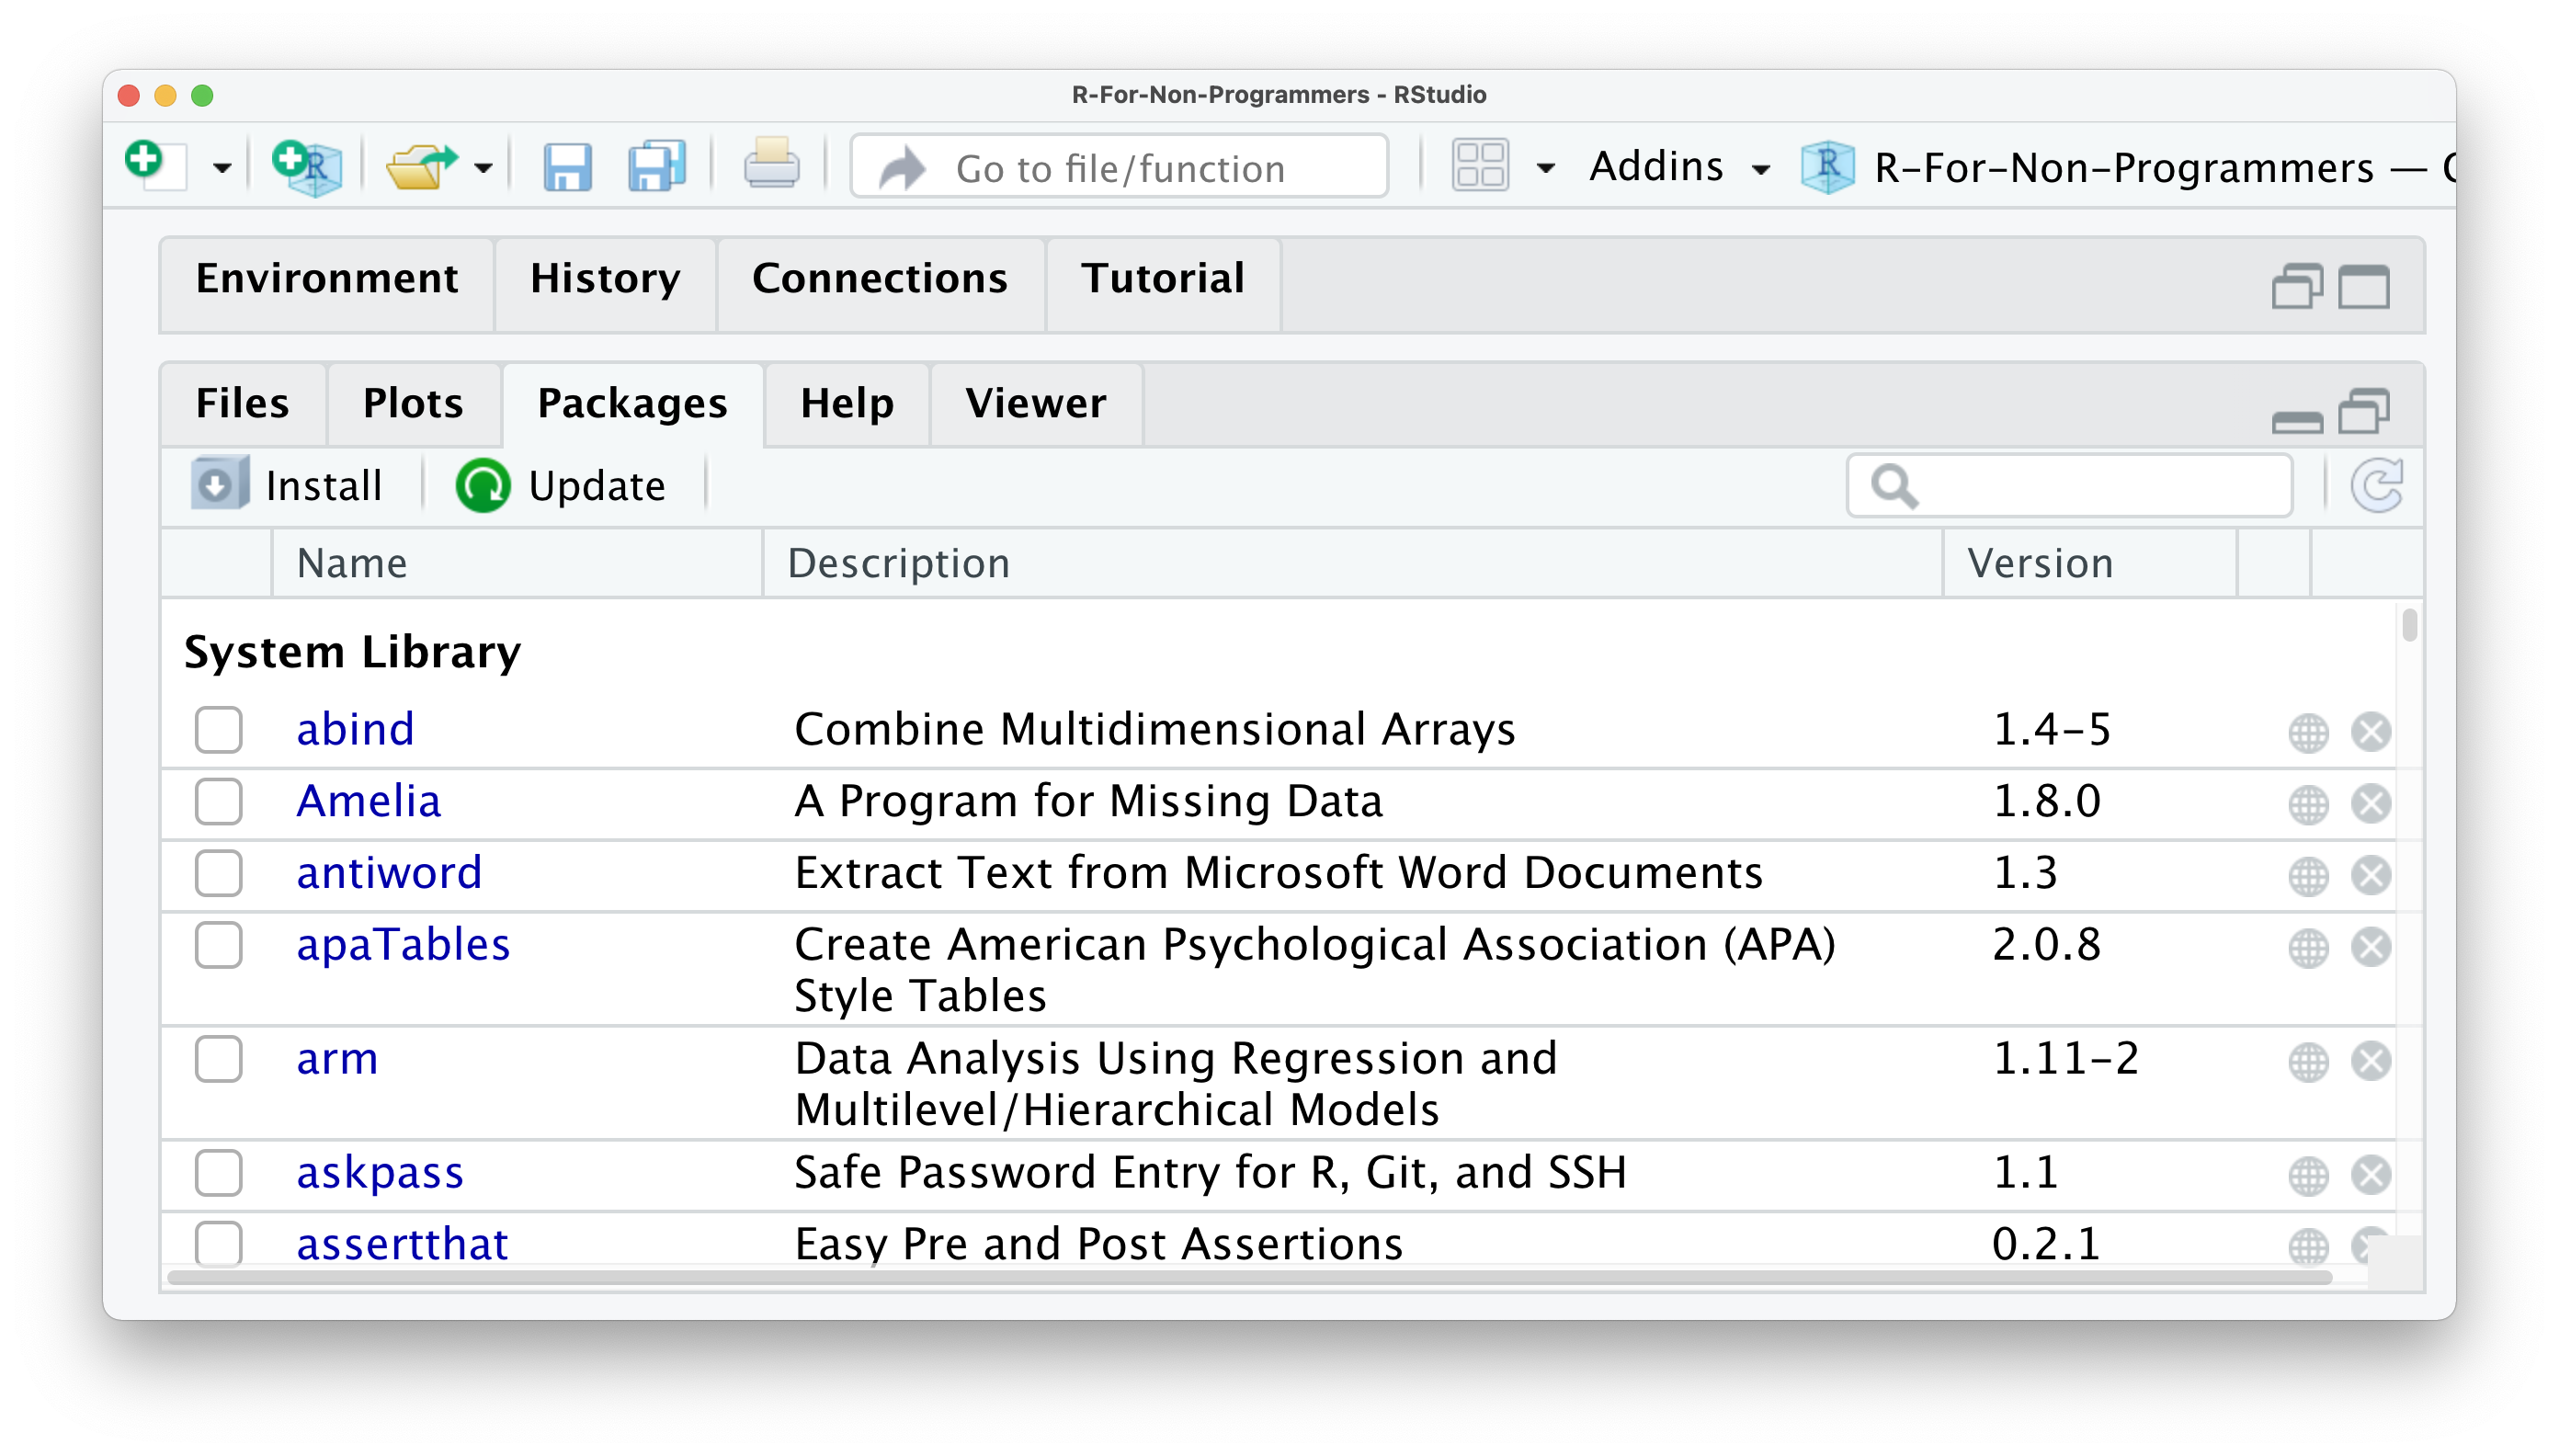
\includegraphics{images/chapter_04_img/05_files_plots_etc/03_rstudio_packages.png}

If you are in dire need of help, RStudio provides you with a \emph{Help}
pane. You can search for specific topics, such as how certain
computations work. The \emph{Help} pane also has documentation on
different datasets that are included in \emph{R}, RStudio or \emph{R
packages} you have installed. If you want a more comprehensive overview
of how you can find help, have a look at CRAN's
\href{https://www.r-project.org/help.html}{`Getting Help with R'}
webpage.

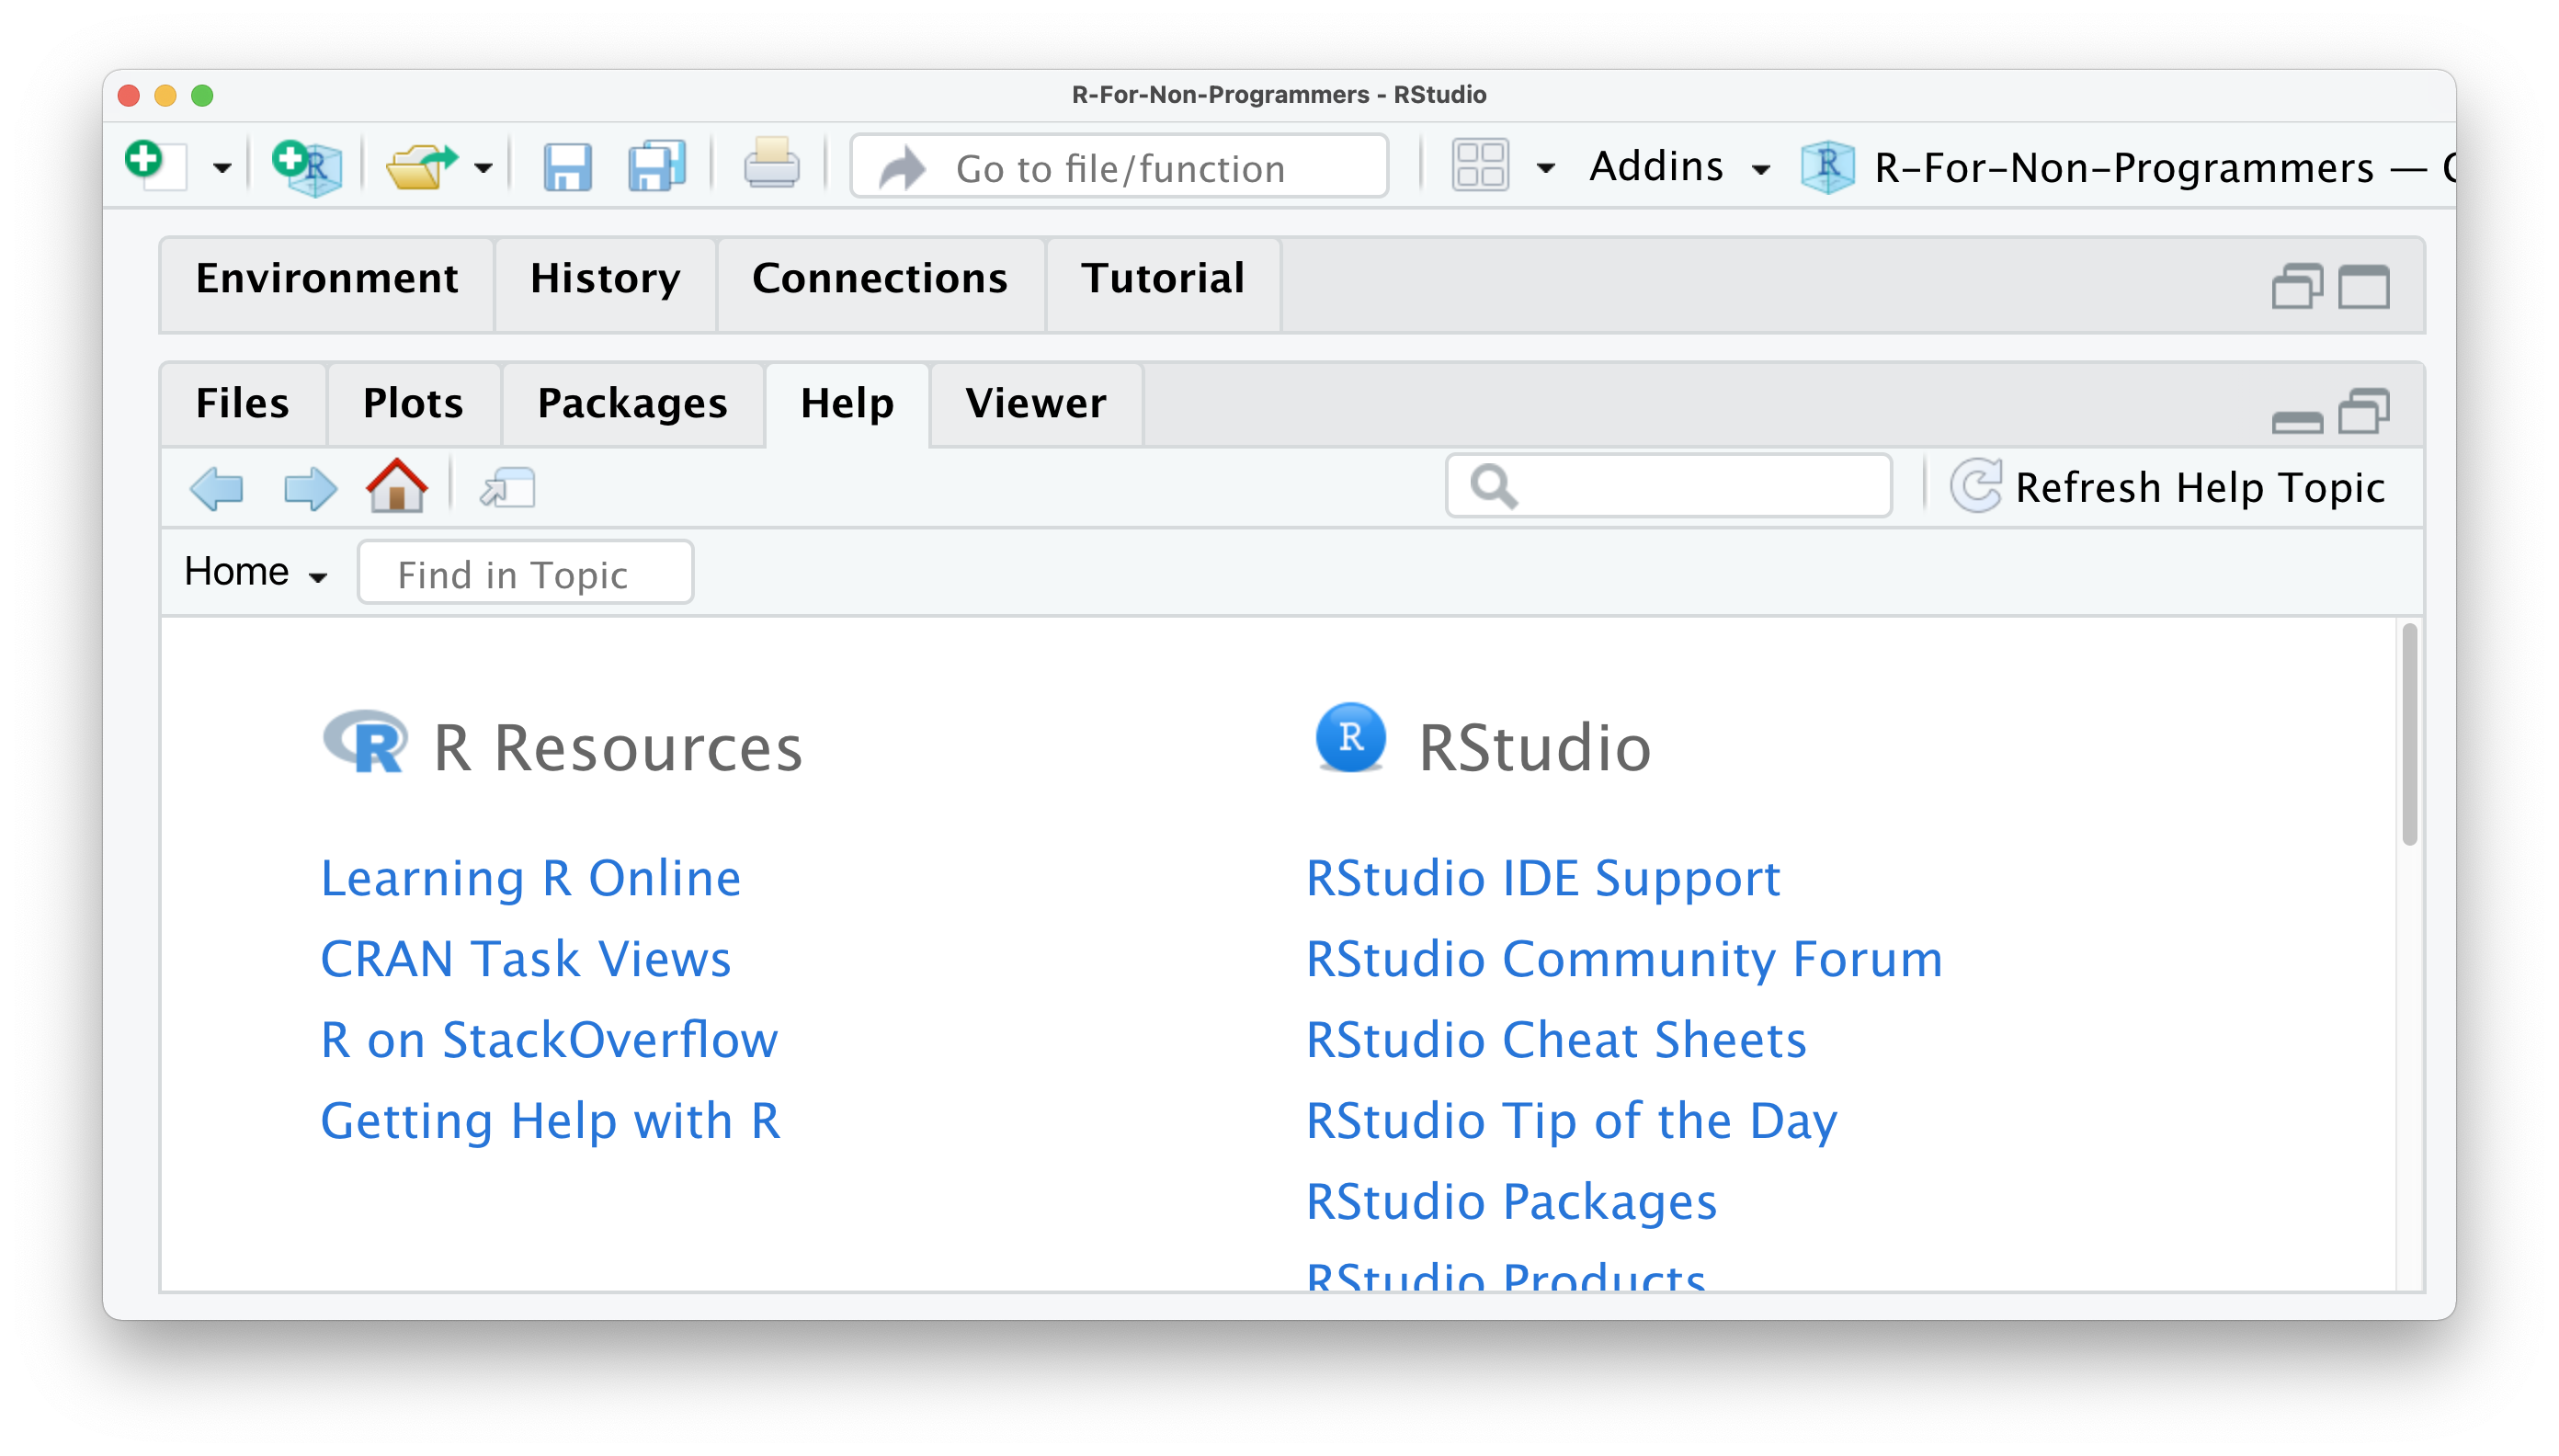
\includegraphics{images/chapter_04_img/05_files_plots_etc/04_rstudio_help.png}

So, for example, if you want to know what the \texttt{mtcars} dataset
is, you can either use the search window in the \emph{Help} pane or,
much easier, use a \texttt{?} in the console to search for it:

\begin{Shaded}
\begin{Highlighting}[]
\CommentTok{\# Type a \textquotesingle{}?\textquotesingle{} followed by the name of a dataset/function/etc.}
\CommentTok{\# to look up helpful information about it.}
\NormalTok{?mtcars}
\end{Highlighting}
\end{Shaded}

This will open the \emph{Help} pane and give you more information about
this dataset:

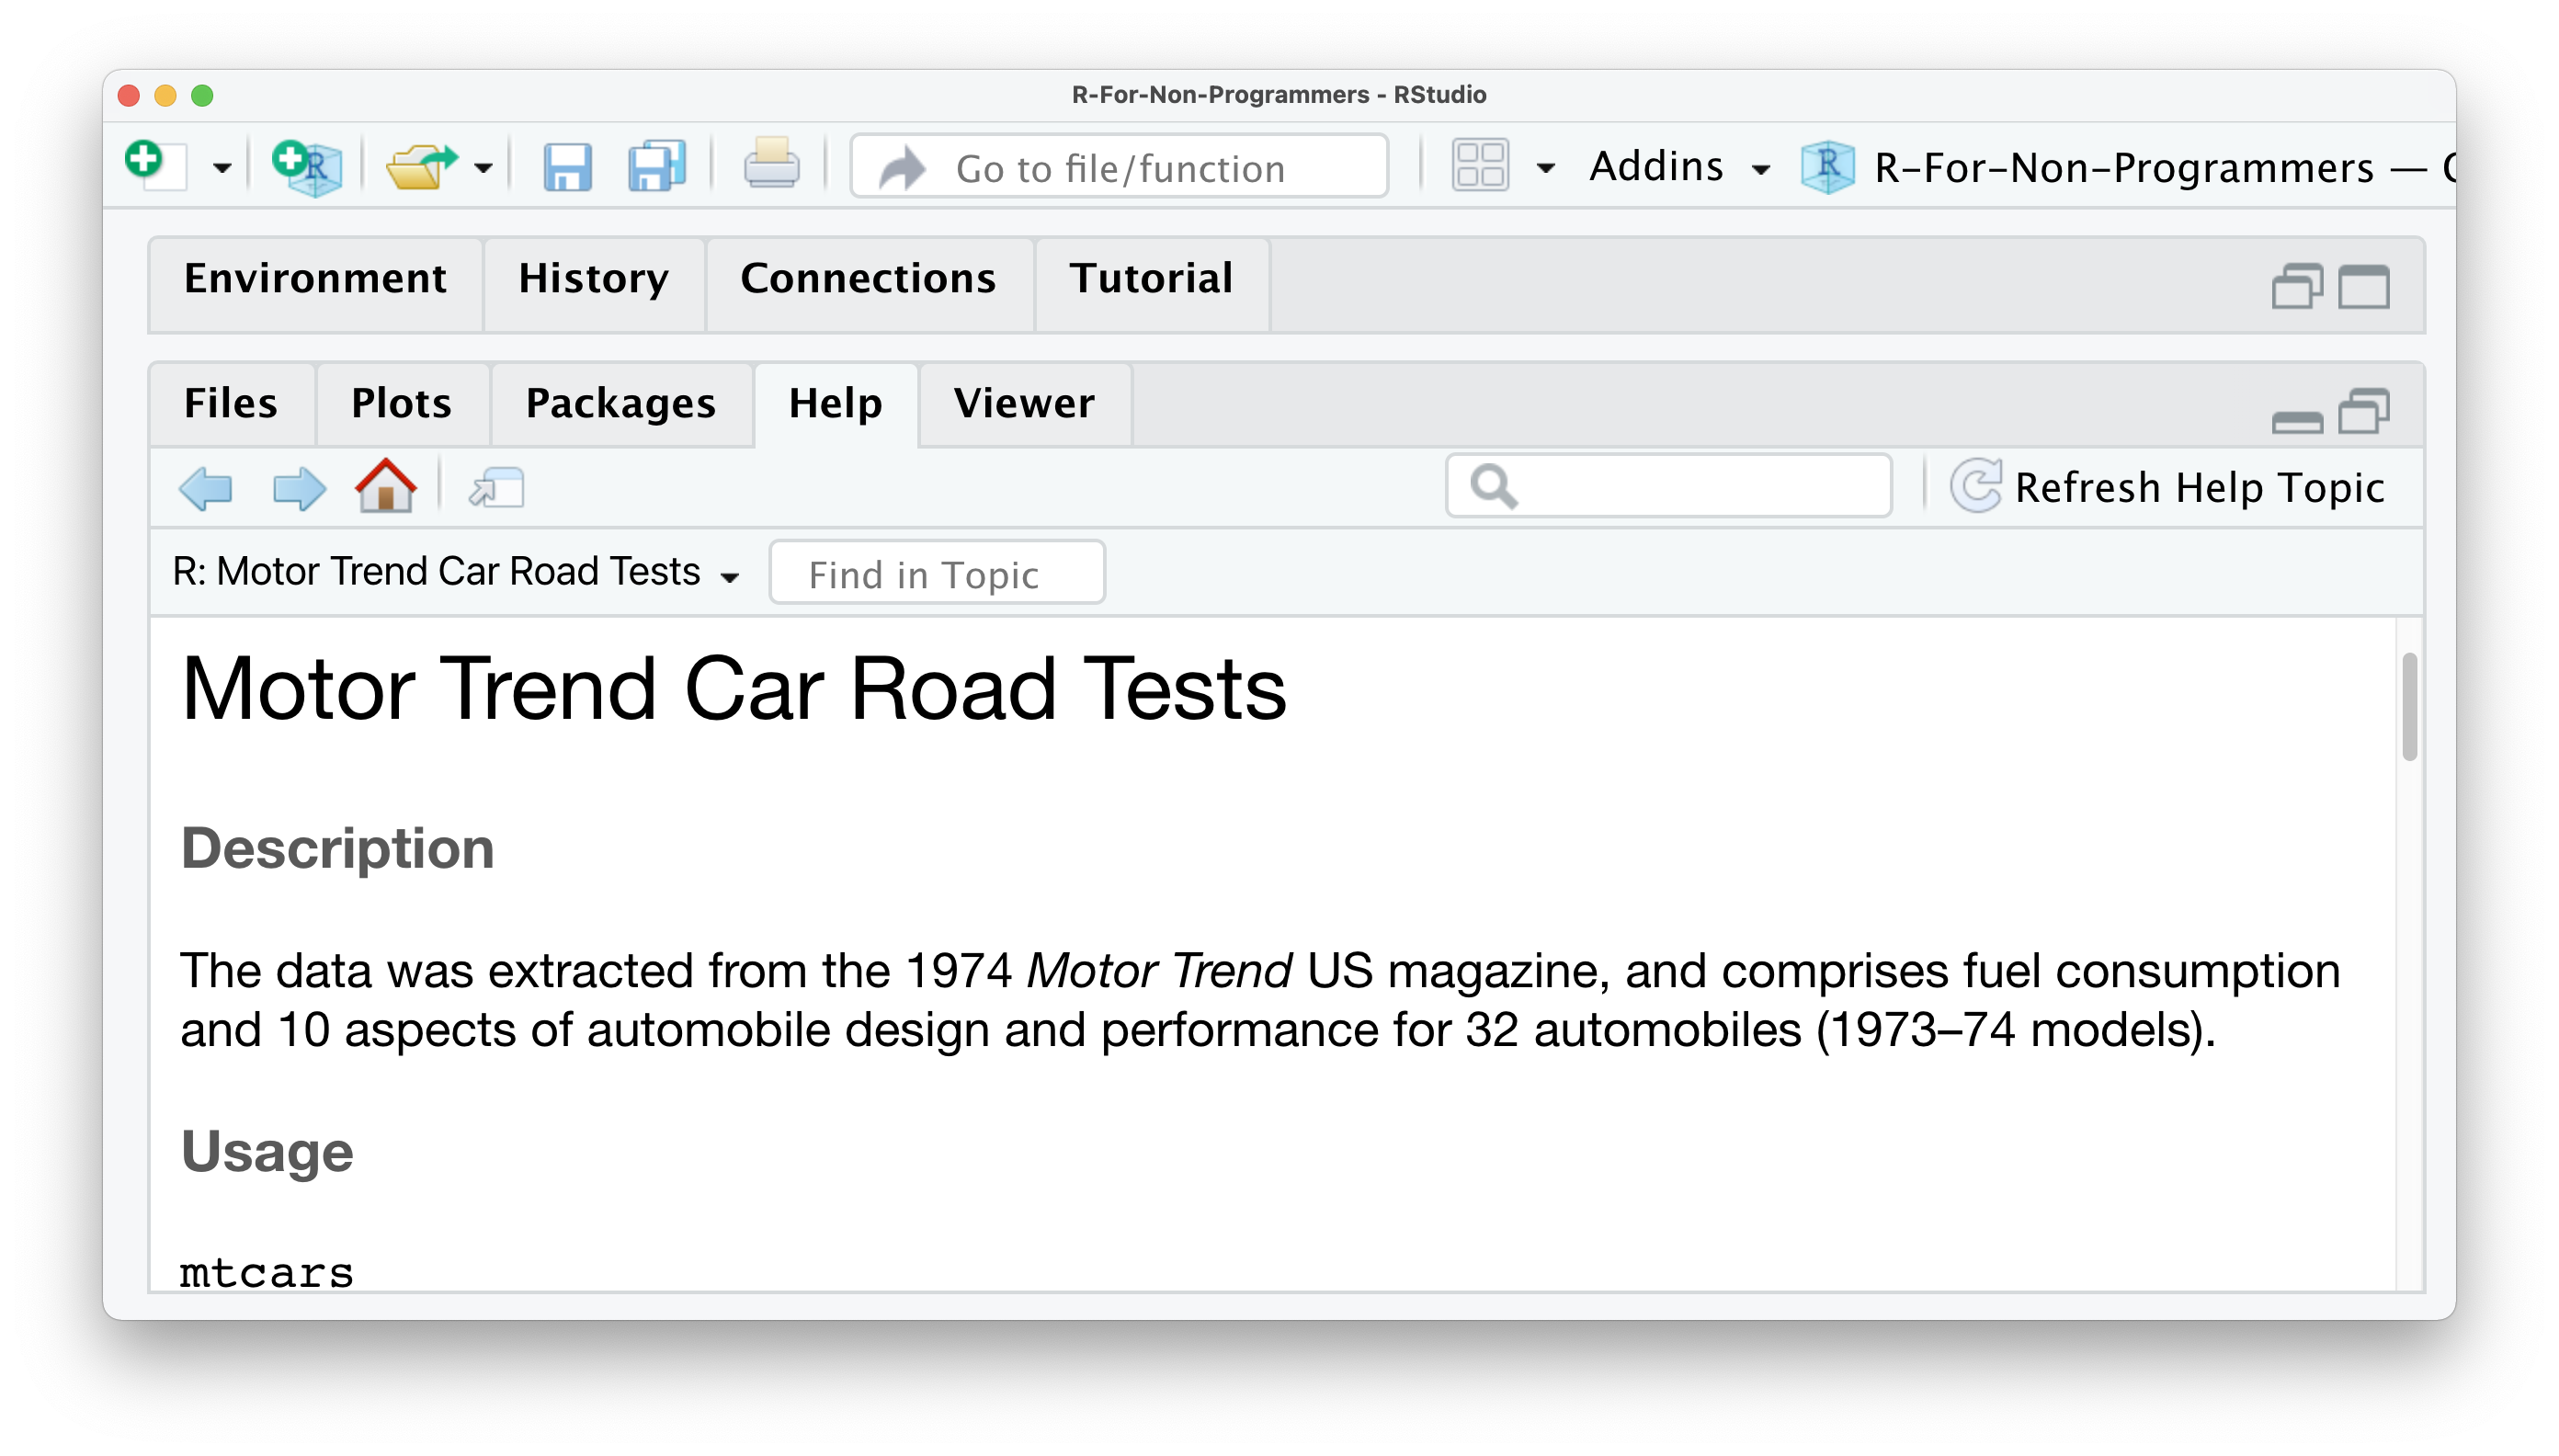
\includegraphics{images/chapter_04_img/05_files_plots_etc/04_rstudio_help_mtcars.png}

There are many different ways of how you can find help with your coding
beyond RStudio and this book. My top three platforms to find solutions
to my programming problems are:

\begin{itemize}
\item
  \href{https://www.google.com}{Google}
\item
  \href{https://stackoverflow.com}{stackoverflow.com}
\item
  \href{https://twitter.com/home}{X/Twitter} (with
  \href{https://twitter.com/hashtag/rstats}{\#RStats})
\end{itemize}

Lastly, we have the \emph{Viewer} pane. Not every data visualisation we
create in \emph{R} is a static image. You can create dynamic data
visualisations or even websites with \emph{R}. This type of content is
displayed in the \emph{Viewer} pane rather than in the \emph{Plots}
pane. Often, these visualisations are based on HTML and other web-based
programming languages. As such, it is easy to open them in your browser.
However, in this book, we mainly focus on two-dimensional static plots,
which are the ones you likely need most of the time, either for your
assignments, thesis, or publication.

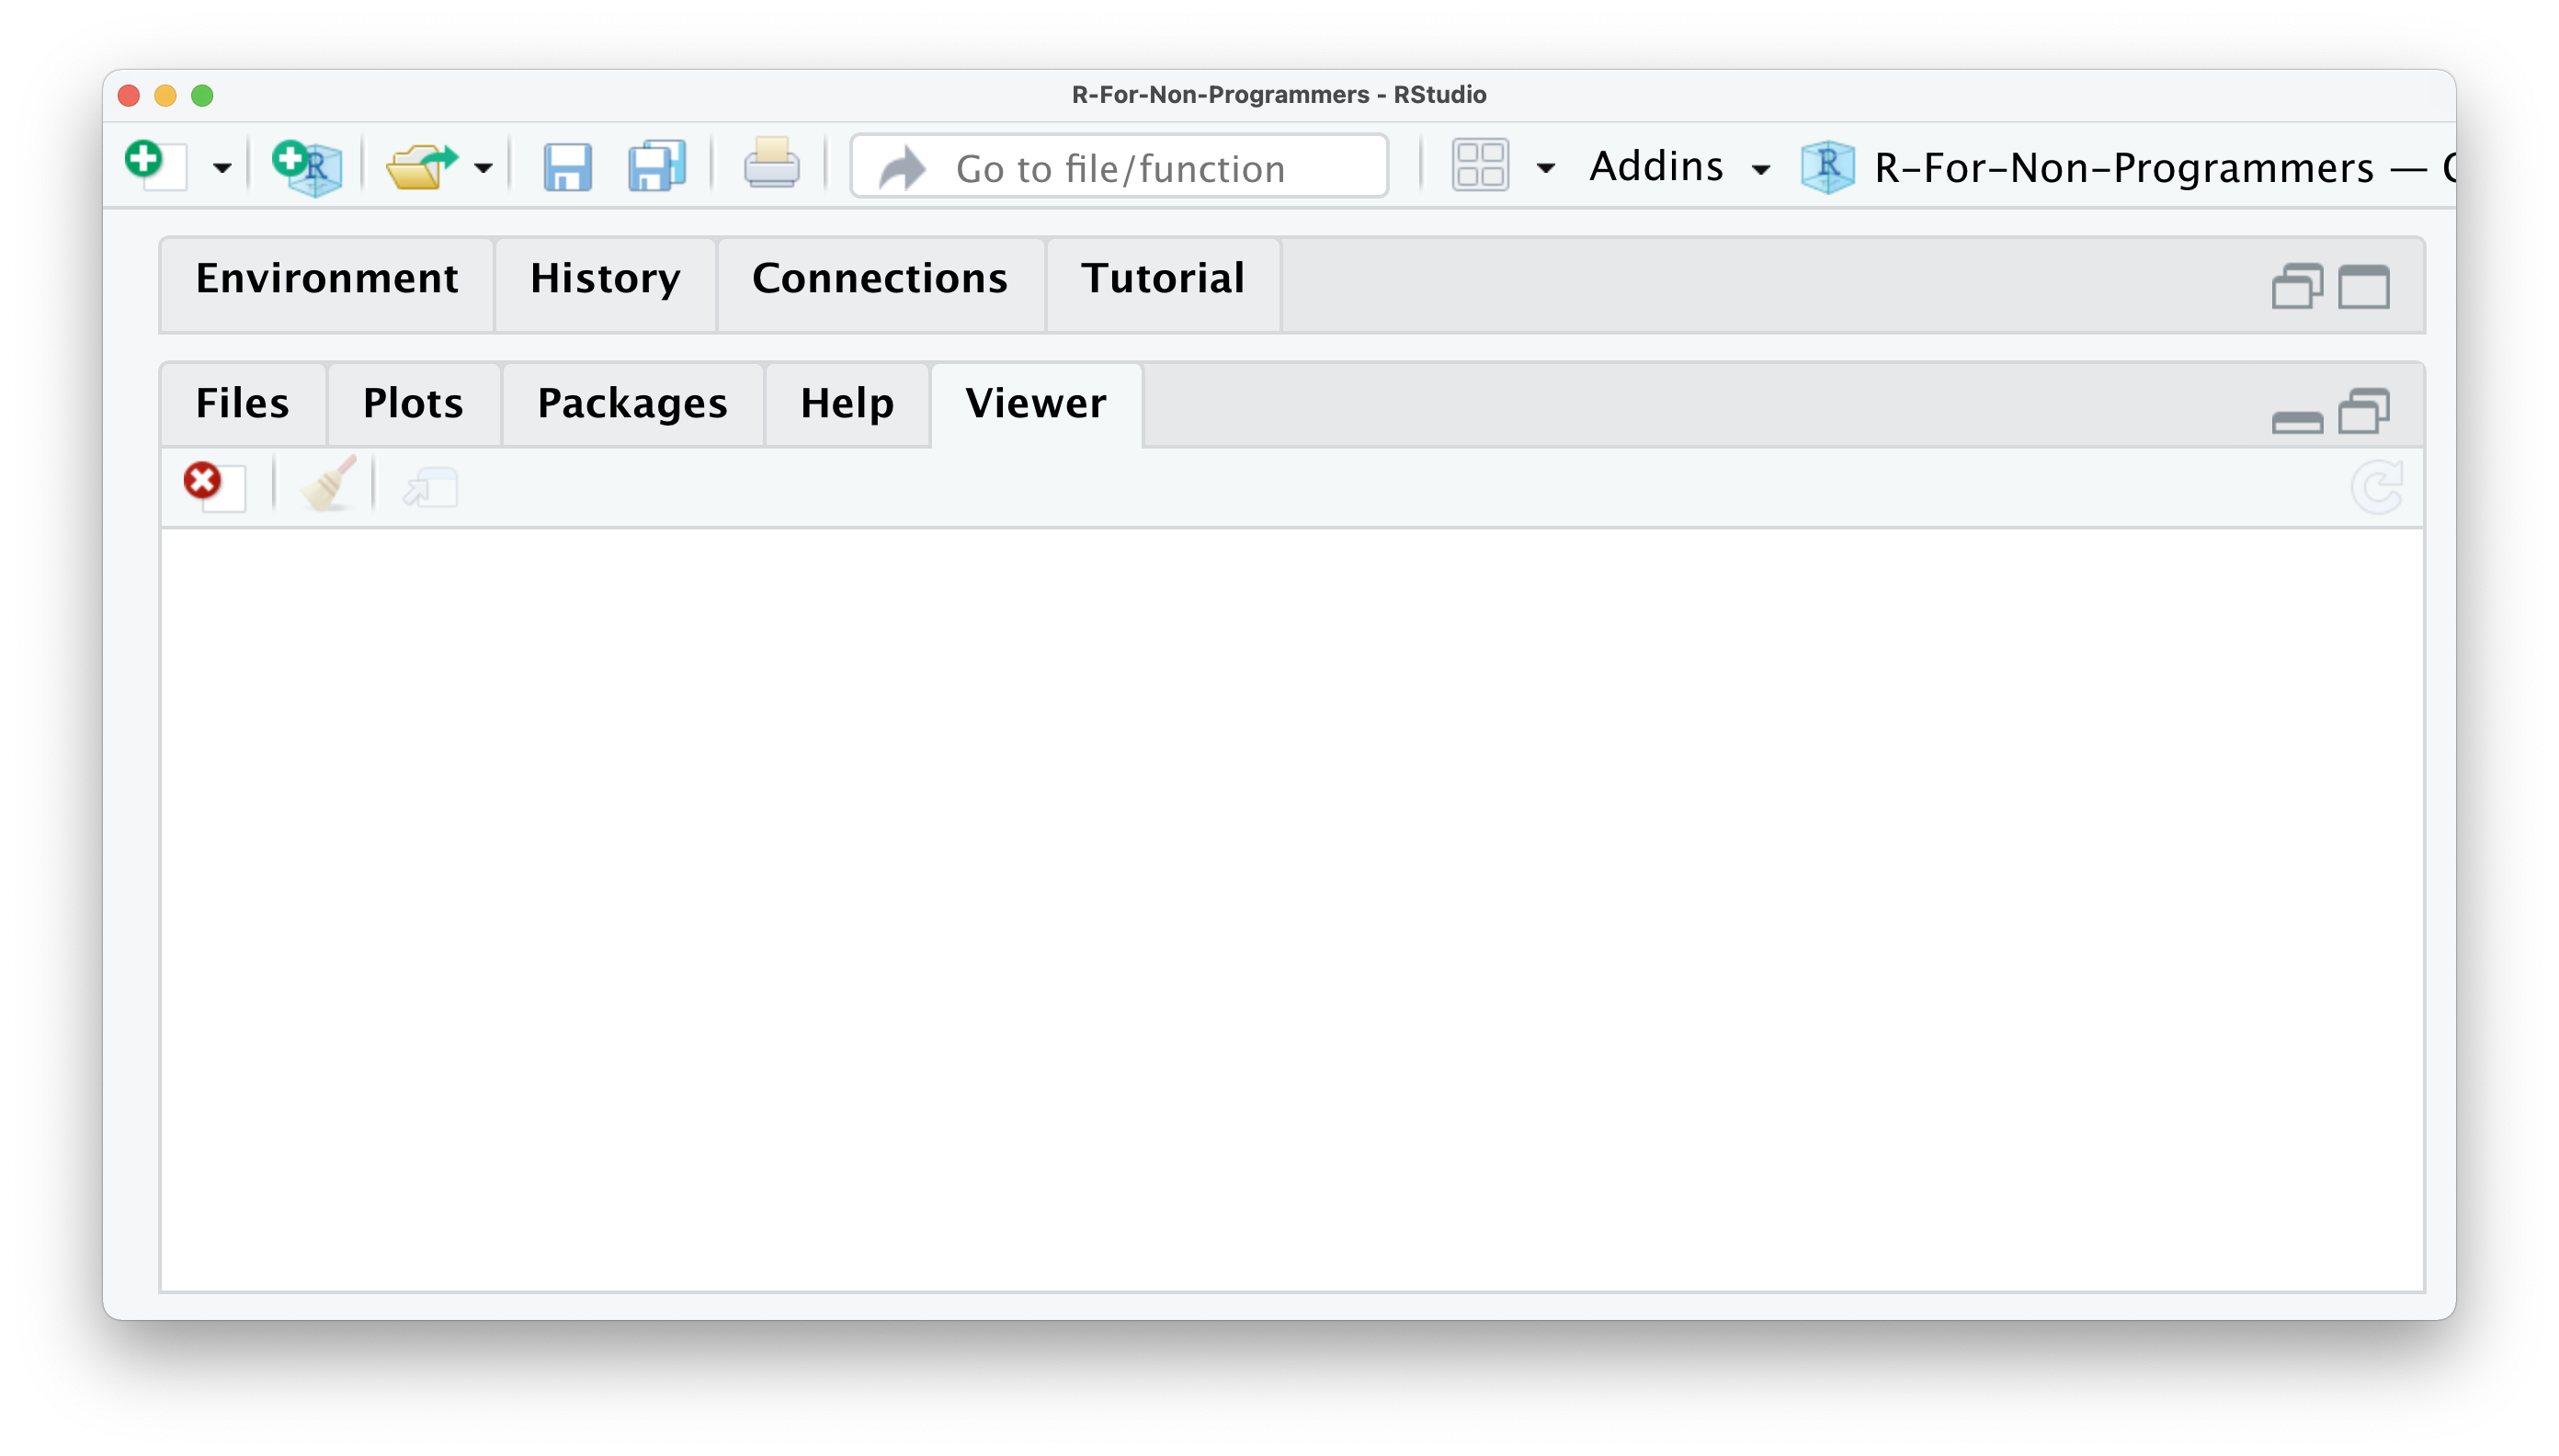
\includegraphics{images/chapter_04_img/05_files_plots_etc/05_rstudio_viewer.png}

\section{Customise your user
interface}\label{sec-customise-your-user-interface}

As a last remark in this chapter, I would like to make you aware that
you can modify each window. There are three basic adjustments you can
make:

\begin{itemize}
\item
  Hide panes by clicking on the window symbol in the top right corner of
  each window,
\item
  Resize panes by dragging the border of a window horizontally or
  vertically or
\item
  Add and remove panes by going to
  \texttt{RStudio\ \textgreater{}\ Preferences\ \textgreater{}\ Pane\ Layout},
  or use the keyboard shortcut \texttt{⌘\ +\ ,} if you are on a Mac.
  Unfortunately, there is no default shortcut for PC users.
\end{itemize}

If you want a fully customised experience, you can also alter the colour
scheme of RStudio itself
(\texttt{RStudio\ \textgreater{}\ Preferences\ \textgreater{}\ Appearance}).
If the themes offered are not enough for you, you can create a custom
theme
\href{https://tmtheme-editor.herokuapp.com/\#!/editor/theme/Monokai}{here}.

\bookmarksetup{startatroot}

\chapter{\texorpdfstring{\emph{R} Basics: The very
fundamentals}{R Basics: The very fundamentals}}\label{sec-r-basics-the-very-fundamentals}

After a likely tedious installation of \emph{R} and RStudio, as well as
a somewhat detailed introduction to the RStudio interface, you are
finally ready to \emph{`do'} things. By \emph{`doing'}, I mean
\emph{`coding'}. The term \emph{`coding'} in itself can instil fear in
some of you, but you only need one skill to do it: Writing. As mentioned
earlier, learning coding or programming means learning a new language.
However, once you have the basic grammar down, you already can
communicate quite a bit. In this section, we will explore the
fundamentals of \emph{R}. These build the foundation for everything that
follows. After that, we dive right into some analysis.

\section{\texorpdfstring{Basic computations in
\emph{R}}{Basic computations in R}}\label{sec-basic-computations-in-r}

The most basic computation you can do in \emph{R} is arithmetic
operations. In other words, addition, subtraction, multiplication,
division, exponentiation and extraction of roots. In short, \emph{R} can
be used like your pocket calculator, or more likely the one you have on
your phone. For example, in Section~\ref{sec-the-console-window} we
already performed an addition. Thus, it might not come as a surprise how
their equivalents work in \emph{R}. Let's take a look at the following
examples:

\begin{Shaded}
\begin{Highlighting}[]
\CommentTok{\# Addition}
\DecValTok{10} \SpecialCharTok{+} \DecValTok{5}
\end{Highlighting}
\end{Shaded}

\begin{verbatim}
[1] 15
\end{verbatim}

\begin{Shaded}
\begin{Highlighting}[]
\CommentTok{\# Subtraction}
\DecValTok{10} \SpecialCharTok{{-}} \DecValTok{5}
\end{Highlighting}
\end{Shaded}

\begin{verbatim}
[1] 5
\end{verbatim}

\begin{Shaded}
\begin{Highlighting}[]
\CommentTok{\# Multiplication}
\DecValTok{10} \SpecialCharTok{*} \DecValTok{5}
\end{Highlighting}
\end{Shaded}

\begin{verbatim}
[1] 50
\end{verbatim}

\begin{Shaded}
\begin{Highlighting}[]
\CommentTok{\# Division}
\DecValTok{10} \SpecialCharTok{/} \DecValTok{5}
\end{Highlighting}
\end{Shaded}

\begin{verbatim}
[1] 2
\end{verbatim}

\begin{Shaded}
\begin{Highlighting}[]
\CommentTok{\# Exponentiation}
\DecValTok{10} \SpecialCharTok{\^{}} \DecValTok{2}
\end{Highlighting}
\end{Shaded}

\begin{verbatim}
[1] 100
\end{verbatim}

\begin{Shaded}
\begin{Highlighting}[]
\CommentTok{\# Square root}
\FunctionTok{sqrt}\NormalTok{(}\DecValTok{10}\NormalTok{)}
\end{Highlighting}
\end{Shaded}

\begin{verbatim}
[1] 3.162278
\end{verbatim}

They all look fairly straightforward except for the extraction of roots.
As you probably know, extracting the root would typically mean we use
the symbol \(\sqrt{}\) on our calculator. To compute the square root in
\emph{R}, we have to use a function instead to perform the computation.
So we first put the name of the function \texttt{sqrt} and then the
value \texttt{10} within parenthesis \texttt{()}. This results in the
following code: \texttt{sqrt(10)}. If we were to write this down in our
report, we would write \(\sqrt[2]{10}\).

Functions are an essential part of \emph{R} and programming in general.
You will learn more about them in Section~\ref{sec-functions}. Besides
arithmetic operations, there are also logical queries you can perform.
Logical queries always return either the value \texttt{TRUE} or
\texttt{FALSE}. Here are some examples which make this clearer:

\begin{Shaded}
\begin{Highlighting}[]
\CommentTok{\#1 Is it TRUE or FALSE?}
\DecValTok{1} \SpecialCharTok{==} \DecValTok{1}
\end{Highlighting}
\end{Shaded}

\begin{verbatim}
[1] TRUE
\end{verbatim}

\begin{Shaded}
\begin{Highlighting}[]
\CommentTok{\#2 Is 45 bigger than 55?}
\DecValTok{45} \SpecialCharTok{\textgreater{}} \DecValTok{55}
\end{Highlighting}
\end{Shaded}

\begin{verbatim}
[1] FALSE
\end{verbatim}

\begin{Shaded}
\begin{Highlighting}[]
\CommentTok{\#3 Is 1982 bigger or equal to 1982?}
\DecValTok{1982} \SpecialCharTok{\textgreater{}=} \DecValTok{1982}
\end{Highlighting}
\end{Shaded}

\begin{verbatim}
[1] TRUE
\end{verbatim}

\begin{Shaded}
\begin{Highlighting}[]
\CommentTok{\#4 Are these two words NOT the same?}
\StringTok{"Friends"} \SpecialCharTok{!=} \StringTok{"friends"}
\end{Highlighting}
\end{Shaded}

\begin{verbatim}
[1] TRUE
\end{verbatim}

\begin{Shaded}
\begin{Highlighting}[]
\CommentTok{\#5 Are these sentences the same?}
\StringTok{"I love statistics"} \SpecialCharTok{==} \StringTok{"I love statistícs"}
\end{Highlighting}
\end{Shaded}

\begin{verbatim}
[1] FALSE
\end{verbatim}

Reflecting on these examples, you might notice three important aspects
of logical queries:

\begin{enumerate}
\def\labelenumi{\arabic{enumi}.}
\tightlist
\item
  We have to use \texttt{==} instead of \texttt{=},
\item
  We can compare non-numerical values, i.e.~text, which is also known as
  \texttt{character} values, with each other,
\item
  The devil is in the details (consider \#5).
\end{enumerate}

One of the most common mistakes of \emph{R} novices is the confusion
around the \texttt{==} and \texttt{=} notation. While \texttt{==}
represents \texttt{equal\ to}, \texttt{=} is used to assign a value to
an object (for more details on assignments see
Section~\ref{sec-assigning-values-to-objects}. However, in practice,
most \emph{R} programmers tend to avoid \texttt{=} since it can easily
lead to confusion with \texttt{==}. As such, you can strike \texttt{=}
out of your \emph{R} vocabulary for now.

There are many different logical operations you can perform.
Table~\ref{tbl-logical-operators-r} lists the most frequently used
logical operators for your reference. These will become important, for
example when we filter our data for analysis, e.g.~include only female
or male participants.

\begingroup
\fontsize{12.0pt}{14.4pt}\selectfont

\begin{longtable}{cl}

\caption{\label{tbl-logical-operators-r}Logical operators in R}

\tabularnewline

\toprule
Operator & Description \\ 
\midrule\addlinespace[2.5pt]
== & is equal to \\ 
!= & is not equal to \\ 
>= & is bigger or equal to \\ 
> & is bigger than \\ 
<= & is smaller or equal to \\ 
< & is smaller than \\ 
a | b & a or b \\ 
a \& b & a and b \\ 
!a & is not a \\ 
\bottomrule

\end{longtable}

\endgroup

\section{Assigning values to objects:
`\textless-'}\label{sec-assigning-values-to-objects}

Another common task you will perform is assigning values to an object.
An object can be many different things:

\begin{itemize}
\item
  a dataset,
\item
  the results of a computation,
\item
  a plot,
\item
  a series of numbers,
\item
  a list of names,
\item
  a function,
\item
  etc.
\end{itemize}

In short, an object is an umbrella term for many different things which
form part of your data analysis. For example, objects are handy when
storing results that you want to process further in later analytical
steps. We have to use the assign operator \texttt{\textless{}-} to
assign a value to an object. Let's have a look at an example.

\begin{Shaded}
\begin{Highlighting}[]
\CommentTok{\# I have a friend called "Fiona"}
\NormalTok{friends }\OtherTok{\textless{}{-}} \StringTok{"Fiona"}
\end{Highlighting}
\end{Shaded}

In this example, I created an object called \texttt{friends} and added
\texttt{"Fiona"} to it. Since \texttt{"Fiona"} represents a
\texttt{string}, we need to use \texttt{""}. So, if you wanted to read
this line of code, you would say, `\texttt{friends} gets the value
\texttt{"Fiona"}'. Alternatively, you could also say `\texttt{"Fiona"}
is assigned to \texttt{friends}'.

If you look into your environment pane, you will find the object
\texttt{friends}. You can see it carries the value \texttt{"Fiona"}. We
can also print values of an object in the console by simply typing the
name of the object \texttt{friends} and hit \texttt{Return}.

\begin{Shaded}
\begin{Highlighting}[]
\CommentTok{\# Who are my friends?}
\NormalTok{friends}
\end{Highlighting}
\end{Shaded}

\begin{verbatim}
[1] "Fiona"
\end{verbatim}

Sadly, it seems I only have one friend. Luckily we can add some more,
not the least to make me feel less lonely. To create objects with
multiple values, we can use the function \texttt{c()}, which stands for
`concatenate'. The Cambridge Dictionary (2021) defines this word as
follows:

\begin{quote}
`\textbf{\emph{concatenate}}',

\emph{to put things together as a connected series.}
\end{quote}

Let's concatenate some more friends into our \texttt{friends} object.

\begin{Shaded}
\begin{Highlighting}[]
\CommentTok{\# Adding some more friends to my life}
\NormalTok{friends }\OtherTok{\textless{}{-}} \FunctionTok{c}\NormalTok{(}\StringTok{"Fiona"}\NormalTok{,}
             \StringTok{"Lukas"}\NormalTok{,}
             \StringTok{"Ida"}\NormalTok{,}
             \StringTok{"Georg"}\NormalTok{,}
             \StringTok{"Daniel"}\NormalTok{,}
             \StringTok{"Pavel"}\NormalTok{,}
             \StringTok{"Tigger"}\NormalTok{)}

\CommentTok{\# Here are all my friends}
\NormalTok{friends}
\end{Highlighting}
\end{Shaded}

\begin{verbatim}
[1] "Fiona"  "Lukas"  "Ida"    "Georg"  "Daniel" "Pavel"  "Tigger"
\end{verbatim}

To concatenate values into a single object, we need to use a comma
\texttt{,} to separate each value. This is not dissimilar to how we
create lists when writing in English. Otherwise, \emph{R} will report an
error back.

\begin{Shaded}
\begin{Highlighting}[]
\NormalTok{friends }\OtherTok{\textless{}{-}} \FunctionTok{c}\NormalTok{(}\StringTok{"Fiona"} \StringTok{"Ida"}\NormalTok{)}
\end{Highlighting}
\end{Shaded}

\begin{verbatim}
Error in parse(text = input): <text>:1:22: unexpected string constant
1: friends <- c("Fiona" "Ida"
                         ^
\end{verbatim}

\emph{R}'s error messages tend to be very useful and give meaningful
clues to what went wrong. In this case, we can see that something
`\emph{unexpected}' happened, and it shows where our mistake is. You can
also concatenate numbers

Btw, if you add \texttt{()} around your code, you can automatically
print the content of the object to the console. Thus,

\begin{itemize}
\item
  \texttt{(milestones\_of\_my\_life\ \textless{}-\ c(1982,\ 2006,\ 2011,\ 2018,\ 2020))}
  is the same as
\item
  \texttt{milestones\_of\_my\_life\ \textless{}-\ c(1982,\ 2006,\ 2011,\ 2018,\ 2020)}
  followed by \texttt{milestones\_of\_my\_life}.
\end{itemize}

You can copy and paste the following example to illustrate what I
explained.

\begin{Shaded}
\begin{Highlighting}[]
\CommentTok{\# Important years in my life}
\NormalTok{milestones\_of\_my\_life }\OtherTok{\textless{}{-}} \FunctionTok{c}\NormalTok{(}\DecValTok{1982}\NormalTok{, }\DecValTok{2006}\NormalTok{, }\DecValTok{2011}\NormalTok{, }\DecValTok{2018}\NormalTok{, }\DecValTok{2020}\NormalTok{, }\DecValTok{2022}\NormalTok{)}
\NormalTok{milestones\_of\_my\_life}
\end{Highlighting}
\end{Shaded}

\begin{verbatim}
[1] 1982 2006 2011 2018 2020 2022
\end{verbatim}

\begin{Shaded}
\begin{Highlighting}[]
\CommentTok{\# The same as above {-} no second line of code needed}
\NormalTok{(milestones\_of\_my\_life }\OtherTok{\textless{}{-}} \FunctionTok{c}\NormalTok{(}\DecValTok{1982}\NormalTok{, }\DecValTok{2006}\NormalTok{, }\DecValTok{2011}\NormalTok{, }\DecValTok{2018}\NormalTok{, }\DecValTok{2020}\NormalTok{, }\DecValTok{2022}\NormalTok{))}
\end{Highlighting}
\end{Shaded}

\begin{verbatim}
[1] 1982 2006 2011 2018 2020 2022
\end{verbatim}

Finally, we can also concatenate numbers and character values into one
object:

\begin{Shaded}
\begin{Highlighting}[]
\NormalTok{(names\_and\_years }\OtherTok{\textless{}{-}} \FunctionTok{c}\NormalTok{(}\StringTok{"Fiona"}\NormalTok{, }\DecValTok{1988}\NormalTok{, }\StringTok{"Daniel"}\NormalTok{, }\DecValTok{1982}\NormalTok{))}
\end{Highlighting}
\end{Shaded}

\begin{verbatim}
[1] "Fiona"  "1988"   "Daniel" "1982"  
\end{verbatim}

This last example is not necessarily something I would recommend to do,
because it likely leads to undesirable outcomes. For example, if you
look into your environment pane you currently have three objects:
\texttt{friends}, \texttt{milestones\_of\_my\_life}, and
\texttt{names\_and\_years}.

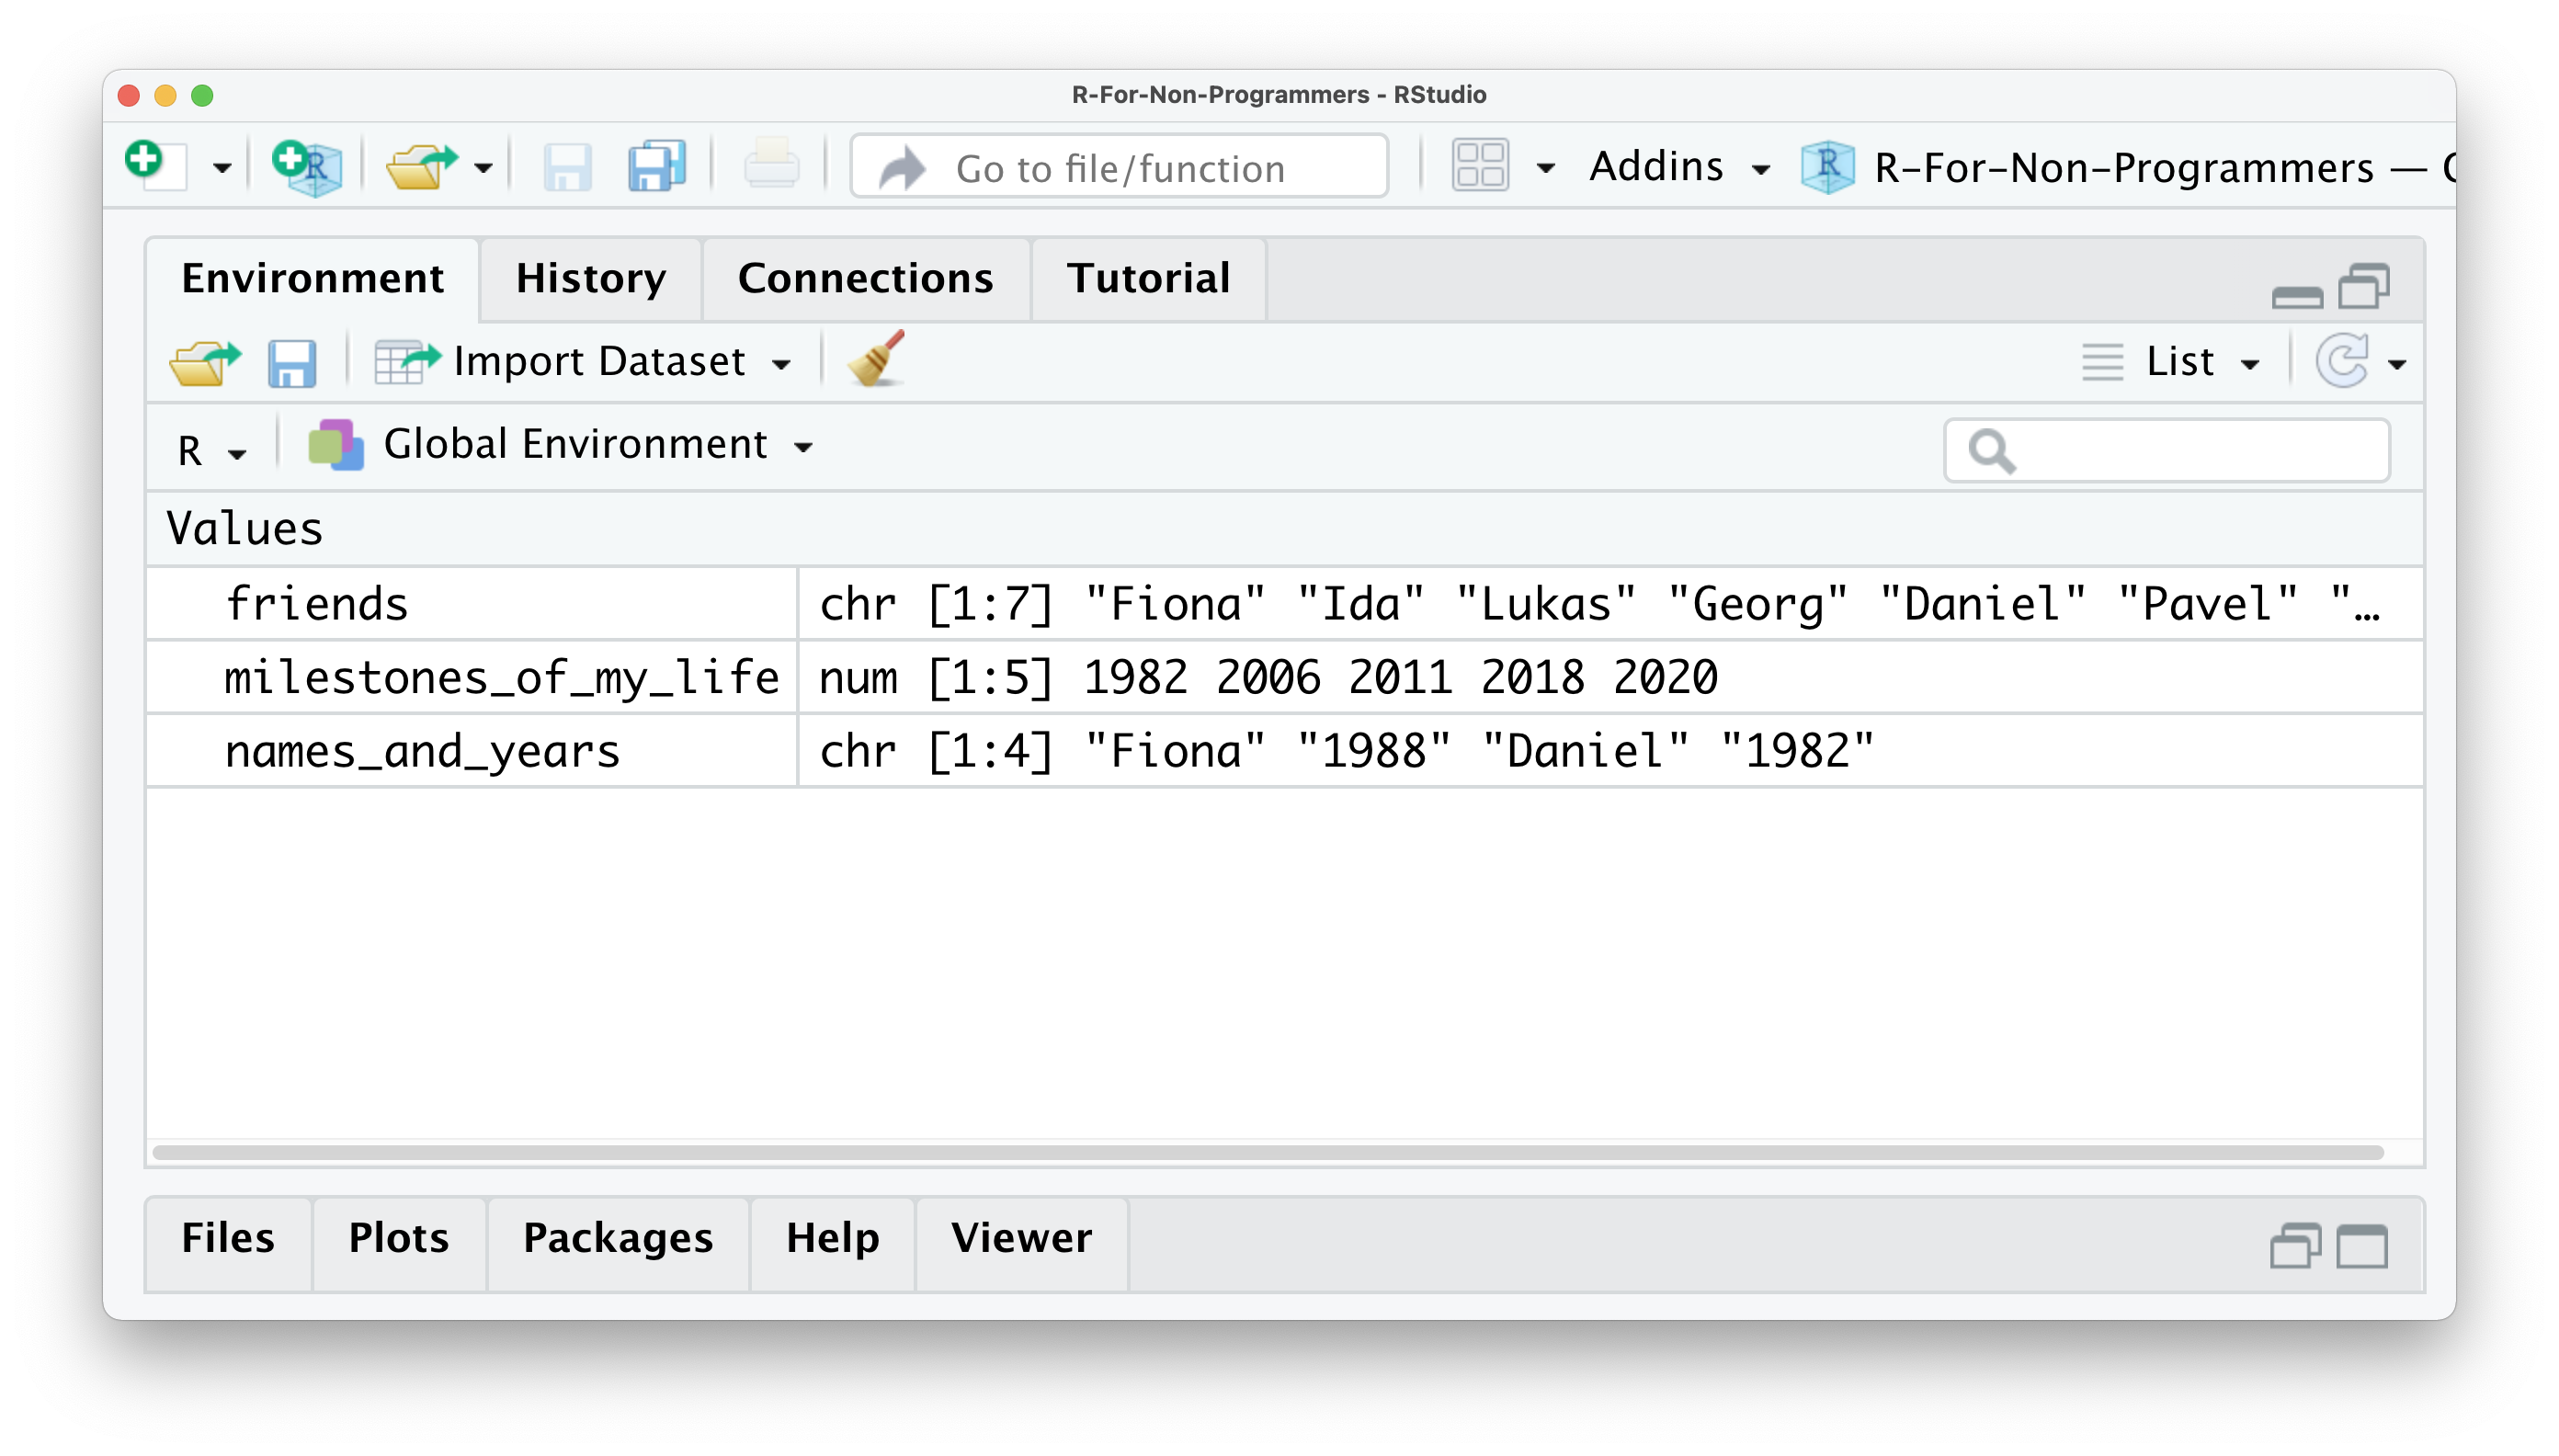
\includegraphics{images/chapter_05_img/01_basic_computation_environment_objects.png}

The \texttt{friends} object shows that all the values inside the object
are classified as \texttt{chr}, which denominates \texttt{character}.
For this object, this is correct because it only includes the names of
my friends. On the other hand, the object
\texttt{milestones\_of\_my\_life} only includes \texttt{numeric} values,
and therefore it says \texttt{num} in the environment pane. However, for
the object \texttt{names\_and\_years} we know we want to have
\texttt{numeric} and \texttt{character} values included. Still, \emph{R}
recognises them as \texttt{character} values because values inside
objects are meant to be of the same type. Remember that in \emph{R,}
numbers can always be interpreted as \texttt{character} and
\texttt{numeric}, but text only can be considered as \texttt{character}
or a \texttt{factor}.

Consequently, mixing different types of data into one object is likely a
bad idea. This is especially true if you want to use the
\texttt{numeric} values for computation. We will return to data types in
Section~\ref{sec-change-data-types} where we learn how to change them,
but for now we should ensure that our objects are all of the same data
type.

However, there is an exception to this rule. `Of course', you might say.
There is one object that can have values of different types: a
\texttt{list}. As the name indicates, a \texttt{list} object holds
several items. These items are usually other objects. In the spirit of
`\href{https://www.imdb.com/title/tt1375666/?ref_=ext_shr_lnk}{Inception}',
you can have lists inside lists, which contain more lists or other
objects.

Let's create a \texttt{list} called \texttt{x\_files} using the
\texttt{list} function and place all our objects inside.

\begin{Shaded}
\begin{Highlighting}[]
\CommentTok{\# This creates our list of objects}
\NormalTok{x\_files }\OtherTok{\textless{}{-}} \FunctionTok{list}\NormalTok{(friends,}
\NormalTok{                milestones\_of\_my\_life,}
\NormalTok{                names\_and\_years)}

\CommentTok{\# Let\textquotesingle{}s have a look what is hidden inside the x\_files}
\NormalTok{x\_files}
\end{Highlighting}
\end{Shaded}

\begin{verbatim}
[[1]]
[1] "Fiona"  "Lukas"  "Ida"    "Georg"  "Daniel" "Pavel"  "Tigger"

[[2]]
[1] 1982 2006 2011 2018 2020 2022

[[3]]
[1] "Fiona"  "1988"   "Daniel" "1982"  
\end{verbatim}

You will notice in this example that I do not use \texttt{""} for each
value in the list. This is because \texttt{friends} is not a
\texttt{character} value, but an object. When we refer to objects, we do
not need quotation marks.

We will encounter \texttt{list} objects quite frequently when we perform
our analysis. Some functions return the results in the format of lists.
This can be very helpful because otherwise our environment pane will be
littered with objects and we would not necessarily know how they relate
to each other, or worse, to which analysis they belong. Looking at the
list item in the environment page (Figure~\ref{fig-img-x-files}), you
can see that the object \texttt{x\_files} is classified as a
\texttt{List\ of\ 3,} and if you click on the blue icon, you can inspect
the different objects inside.

\begin{figure}

\centering{

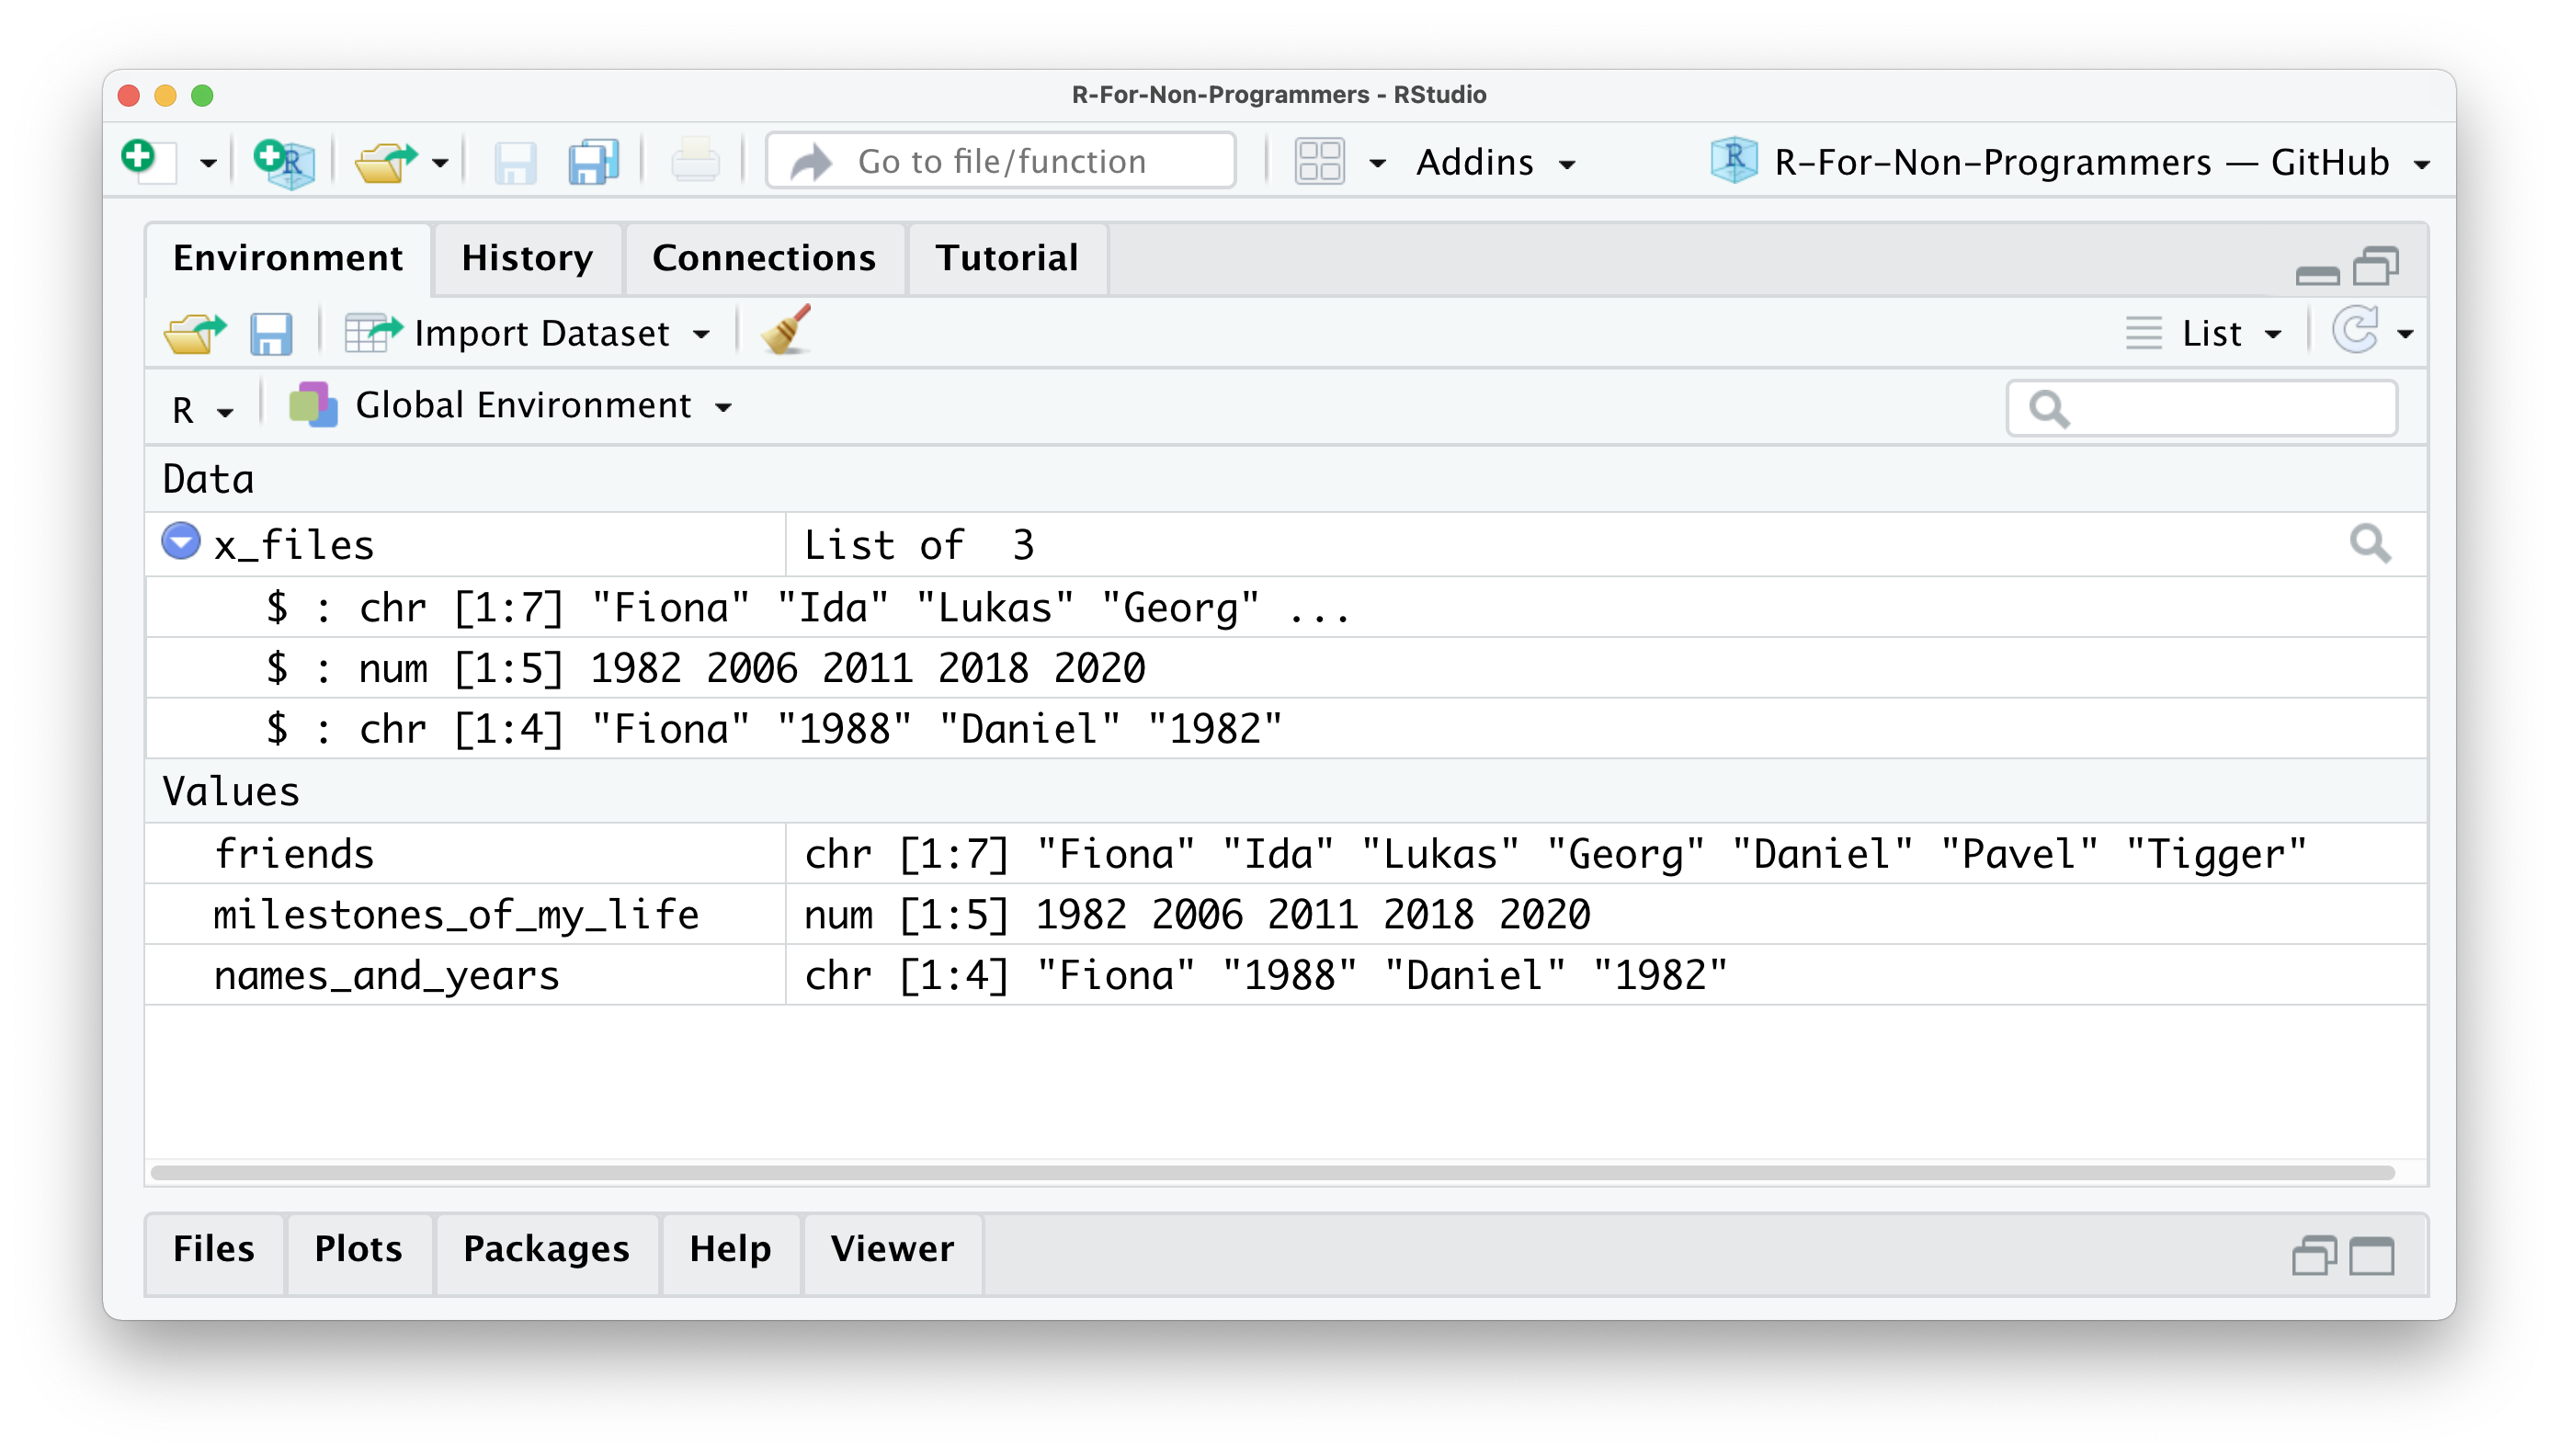
\includegraphics{images/chapter_05_img/02_basic_computation_environment_lists.png}

}

\caption{\label{fig-img-x-files}The environment pane showing our objects
and our list \texttt{x\_files}}

\end{figure}%

In Section~\ref{sec-basic-computations-in-r} , I mentioned that we
should avoid using the \texttt{=} operator and explained that it is used
to assign values to objects. You can, if you want, use \texttt{=}
instead of \texttt{\textless{}-}. They fulfil the same purpose. However,
as mentioned before, it is not wise to do so. Here is an example that
shows that, in principle, it is possible.

\begin{Shaded}
\begin{Highlighting}[]
\CommentTok{\# DO}
\NormalTok{(avengers1 }\OtherTok{\textless{}{-}} \FunctionTok{c}\NormalTok{(}\StringTok{"Iron Man"}\NormalTok{,}
                \StringTok{"Captain America"}\NormalTok{,}
                \StringTok{"Black Widow"}\NormalTok{,}
                \StringTok{"Vision"}\NormalTok{))}
\end{Highlighting}
\end{Shaded}

\begin{verbatim}
[1] "Iron Man"        "Captain America" "Black Widow"     "Vision"         
\end{verbatim}

\begin{Shaded}
\begin{Highlighting}[]
\CommentTok{\# DON\textquotesingle{}T}
\NormalTok{(}\AttributeTok{avengers2 =} \FunctionTok{c}\NormalTok{(}\StringTok{"Iron Man"}\NormalTok{,}
               \StringTok{"Captain America"}\NormalTok{,}
               \StringTok{"Black Widow"}\NormalTok{,}
               \StringTok{"Vision"}\NormalTok{))}
\end{Highlighting}
\end{Shaded}

\begin{verbatim}
[1] "Iron Man"        "Captain America" "Black Widow"     "Vision"         
\end{verbatim}

On a final note, naming your objects is limited. You cannot chose any
name. First, every name needs to start with a letter. Second, you can
only use letters, numbers \texttt{\_} and \texttt{.} as valid components
of the names for your objects (see also Chapter 4.2 in Wickham and
Grolemund 2016). I recommend to establish a naming convention that you
adhere to. Personally I prefer to only user lower-case letters and
\texttt{\_} to separate/connect words. Ideally, you want to keep names
informative, succinct and precise. Here are some examples of what some
might consider good and bad choices for names.

\begin{Shaded}
\begin{Highlighting}[]
\CommentTok{\# Good choices}
\NormalTok{income\_per\_annum}
\NormalTok{open\_to\_exp          }\CommentTok{\# for \textquotesingle{}openness to new experiences\textquotesingle{}}
\NormalTok{soc\_int              }\CommentTok{\# for \textquotesingle{}social integration\textquotesingle{}}
 
\CommentTok{\# Bad choices}
\NormalTok{IncomePerAnnum}
\NormalTok{measurement\_of\_boredom\_of\_watching\_youtube}
\NormalTok{Sleep.per\_monthsIn.hours}
\end{Highlighting}
\end{Shaded}

Ultimately, you need to be able to effectively work with your data and
output. Ideally, this should be true for others as well who want or need
to work with your analysis and data, e.g.~your co-investigator or
supervisor. The same is applies to column names in datasets (see
Section~\ref{sec-colnames-cleaning}). Some more information about coding
style and coding etiquette can be found in
Section~\ref{sec-coding-etiquette}.

\section{Functions}\label{sec-functions}

I used the term `\emph{function}' multiple times, but I never thoroughly
explained what they are and why we need them. In simple terms, functions
are objects. They contain lines of code that someone has written for us
or we have written ourselves. One could say they are code snippets ready
to use. Someone else might see them as shortcuts for our programming.
Functions increase the speed with which we perform our analysis and
write our computations and make our code more readable and reliable.
Consider computing the \texttt{mean} of values stored in the object
\texttt{pocket\_money}.

\begin{Shaded}
\begin{Highlighting}[]
\CommentTok{\# First we create an object that stores our desired values}
\NormalTok{pocket\_money }\OtherTok{\textless{}{-}} \FunctionTok{c}\NormalTok{(}\DecValTok{0}\NormalTok{, }\DecValTok{1}\NormalTok{, }\DecValTok{1}\NormalTok{, }\DecValTok{2}\NormalTok{, }\DecValTok{3}\NormalTok{, }\DecValTok{5}\NormalTok{, }\DecValTok{8}\NormalTok{, }\DecValTok{13}\NormalTok{, }\DecValTok{21}\NormalTok{, }\DecValTok{34}\NormalTok{, }\DecValTok{55}\NormalTok{, }\DecValTok{88}\NormalTok{)}

\CommentTok{\#1 Manually compute the mean}
\NormalTok{total\_sum }\OtherTok{\textless{}{-}} \DecValTok{0} \SpecialCharTok{+} \DecValTok{1} \SpecialCharTok{+} \DecValTok{1} \SpecialCharTok{+} \DecValTok{2} \SpecialCharTok{+} \DecValTok{3} \SpecialCharTok{+} \DecValTok{5} \SpecialCharTok{+} \DecValTok{8} \SpecialCharTok{+} \DecValTok{13} \SpecialCharTok{+} \DecValTok{21} \SpecialCharTok{+} \DecValTok{34} \SpecialCharTok{+} \DecValTok{55} \SpecialCharTok{+} \DecValTok{88}
\NormalTok{total\_sum }\SpecialCharTok{/} \DecValTok{12} \CommentTok{\# There are 12 items in the object}
\end{Highlighting}
\end{Shaded}

\begin{verbatim}
[1] 19.25
\end{verbatim}

\begin{Shaded}
\begin{Highlighting}[]
\CommentTok{\#2 Use a function to compute the mean}
\FunctionTok{mean}\NormalTok{(pocket\_money)}
\end{Highlighting}
\end{Shaded}

\begin{verbatim}
[1] 19.25
\end{verbatim}

\begin{Shaded}
\begin{Highlighting}[]
\CommentTok{\#3 Let\textquotesingle{}s make sure \#1 and \#2 are actually the same}
\NormalTok{total\_sum }\SpecialCharTok{/} \DecValTok{12} \SpecialCharTok{==} \FunctionTok{mean}\NormalTok{(pocket\_money)}
\end{Highlighting}
\end{Shaded}

\begin{verbatim}
[1] TRUE
\end{verbatim}

If we manually compute the mean, we first calculate the sum of all
values in the object \texttt{pocket\_money}\footnote{If you find the
  order of numbers suspicious, it is because it represents the famous
  \href{https://en.wikipedia.org/wiki/Fibonacci_number}{Fibonacci
  sequence}.}. Then we divide it by the number of values in the object,
which is \texttt{12}. This is the traditional way of computing the mean
as we know it from primary school. However, by simply using the function
\texttt{mean()}, we not only write considerably less code, but it is
also much easier to understand because the word \emph{`mean'} does
precisely what we would expect. Which approach do you find easier: Using
the function \texttt{mean()} or computing it by hand?

To further illustrate how functions look like, let's create one
ourselves and call it \texttt{my\_mean}.

\begin{Shaded}
\begin{Highlighting}[]
\NormalTok{my\_mean }\OtherTok{\textless{}{-}} \ControlFlowTok{function}\NormalTok{(numbers)\{}
  \CommentTok{\# Compute the sum of all values in \textquotesingle{}numbers\textquotesingle{}}
\NormalTok{  sum }\OtherTok{\textless{}{-}} \FunctionTok{sum}\NormalTok{(numbers)}
  
  \CommentTok{\# Divide the sum by the number of items in \textquotesingle{}numbers\textquotesingle{}}
\NormalTok{  result }\OtherTok{\textless{}{-}}\NormalTok{ sum}\SpecialCharTok{/}\FunctionTok{length}\NormalTok{(numbers)}
  
  \CommentTok{\# Return the result in the console}
  \FunctionTok{return}\NormalTok{(result)}
\NormalTok{\}}

\FunctionTok{my\_mean}\NormalTok{(pocket\_money)}
\end{Highlighting}
\end{Shaded}

\begin{verbatim}
[1] 19.25
\end{verbatim}

Don't worry if half of this code does not make sense to you. Writing
functions is an advanced \emph{R} skill. However, it is good to know how
functions look on the `inside'. You certainly can see the similarities
between the code we have written before, but instead of using actual
numbers, we work with placeholders like \texttt{numbers}. This way, we
can use a function for different data and do not have to rewrite it
every time. Writing and using functions relates to the skill of
abstraction mentioned in
Section~\ref{sec-programming-languages-enhance-your-conceptual-thinking}.

All functions in \emph{R} share the same structure. They have a
\texttt{name} followed by \texttt{()}. Within these parentheses, we put
\texttt{arguments}, which have specific \texttt{values}. For example, a
generic structure of a function would look something like this:

\begin{Shaded}
\begin{Highlighting}[]
\FunctionTok{name\_of\_function}\NormalTok{(}\AttributeTok{argument\_1 =}\NormalTok{ value\_1,}
                 \AttributeTok{argument\_2 =}\NormalTok{ value\_2,}
                 \AttributeTok{argument\_3 =}\NormalTok{ value\_3)}
\end{Highlighting}
\end{Shaded}

How many arguments there are and what kind of values you can provide is
very much dependent on the function you use. Thus, not every function
takes every value. In the case of \texttt{mean()}, the function takes an
object which holds a sequence of \texttt{numeric} values. It would make
very little sense to compute the mean of our \texttt{friends} object,
because it only contains names. \emph{R} would return an error message:

\begin{Shaded}
\begin{Highlighting}[]
\FunctionTok{mean}\NormalTok{(friends)}
\end{Highlighting}
\end{Shaded}

\begin{verbatim}
Warning in mean.default(friends): argument is not numeric or logical: returning
NA
\end{verbatim}

\begin{verbatim}
[1] NA
\end{verbatim}

\texttt{NA} refers to a value that is \emph{`not available'}. In this
case, \emph{R} tries to compute the mean, but the result is not
available, because the values are not \texttt{numeric} but a
\texttt{character}. In your dataset, you might find values that are
\texttt{NA}, which means there is data missing. If a function attempts a
computation that includes even just a single value that is \texttt{NA},
\emph{R} will return \texttt{NA}. However, there is a way to fix this.
You will learn more about how to deal with \texttt{NA} values in
Section~\ref{sec-dealing-with-missing-data}.

Sometimes you will also get a message from \emph{R} that states
\texttt{NaN}. \texttt{NaN} stands for \emph{`not a number'} and is
returned when something is not possible to compute, for example:

\begin{Shaded}
\begin{Highlighting}[]
\CommentTok{\# Example 1}
\DecValTok{0} \SpecialCharTok{/} \DecValTok{0}
\end{Highlighting}
\end{Shaded}

\begin{verbatim}
[1] NaN
\end{verbatim}

\begin{Shaded}
\begin{Highlighting}[]
\CommentTok{\# Example 2}
\FunctionTok{sqrt}\NormalTok{(}\SpecialCharTok{{-}}\DecValTok{9}\NormalTok{)}
\end{Highlighting}
\end{Shaded}

\begin{verbatim}
Warning in sqrt(-9): NaNs produced
\end{verbatim}

\begin{verbatim}
[1] NaN
\end{verbatim}

\section{\texorpdfstring{\emph{R}
packages}{R packages}}\label{sec-r-packages}

\emph{R} has many built-in functions that we can use right away.
However, some of the most interesting ones are developed by different
programmers, data scientists and enthusiasts. To add more functions to
your repertoire, you can install \emph{R} packages. \emph{R} packages
are a collection of functions that you can download and use for your own
analysis. Throughout this book, you will learn about and use many
different \emph{R} packages to accomplish various tasks. To give you
another analogy,

\begin{itemize}
\item
  \emph{R} is like a global supermarket where everyone can offer their
  products,
\item
  RStudio is like my shopping cart where I can put the products I like,
  and
\item
  \emph{R} packages are the products I can pick from the shelves.
\end{itemize}

Luckily, \emph{R} packages are free to use, so I do not have to bring my
credit card. For me, these additional functions, developed by some of
the most outstanding scientists, is one of many reasons that keeps me
addicted to performing my research in \emph{R}.

\emph{R} packages do not only include functions but often include
datasets and documentation of what each function does. This way, you can
easily try every function right away, even without your own dataset and
read through what each function in the package does.
Figure~\ref{fig-img-r-package-documentation} shows the documentation of
an \emph{R} package called \texttt{ggplot2}.

\begin{figure}

\centering{

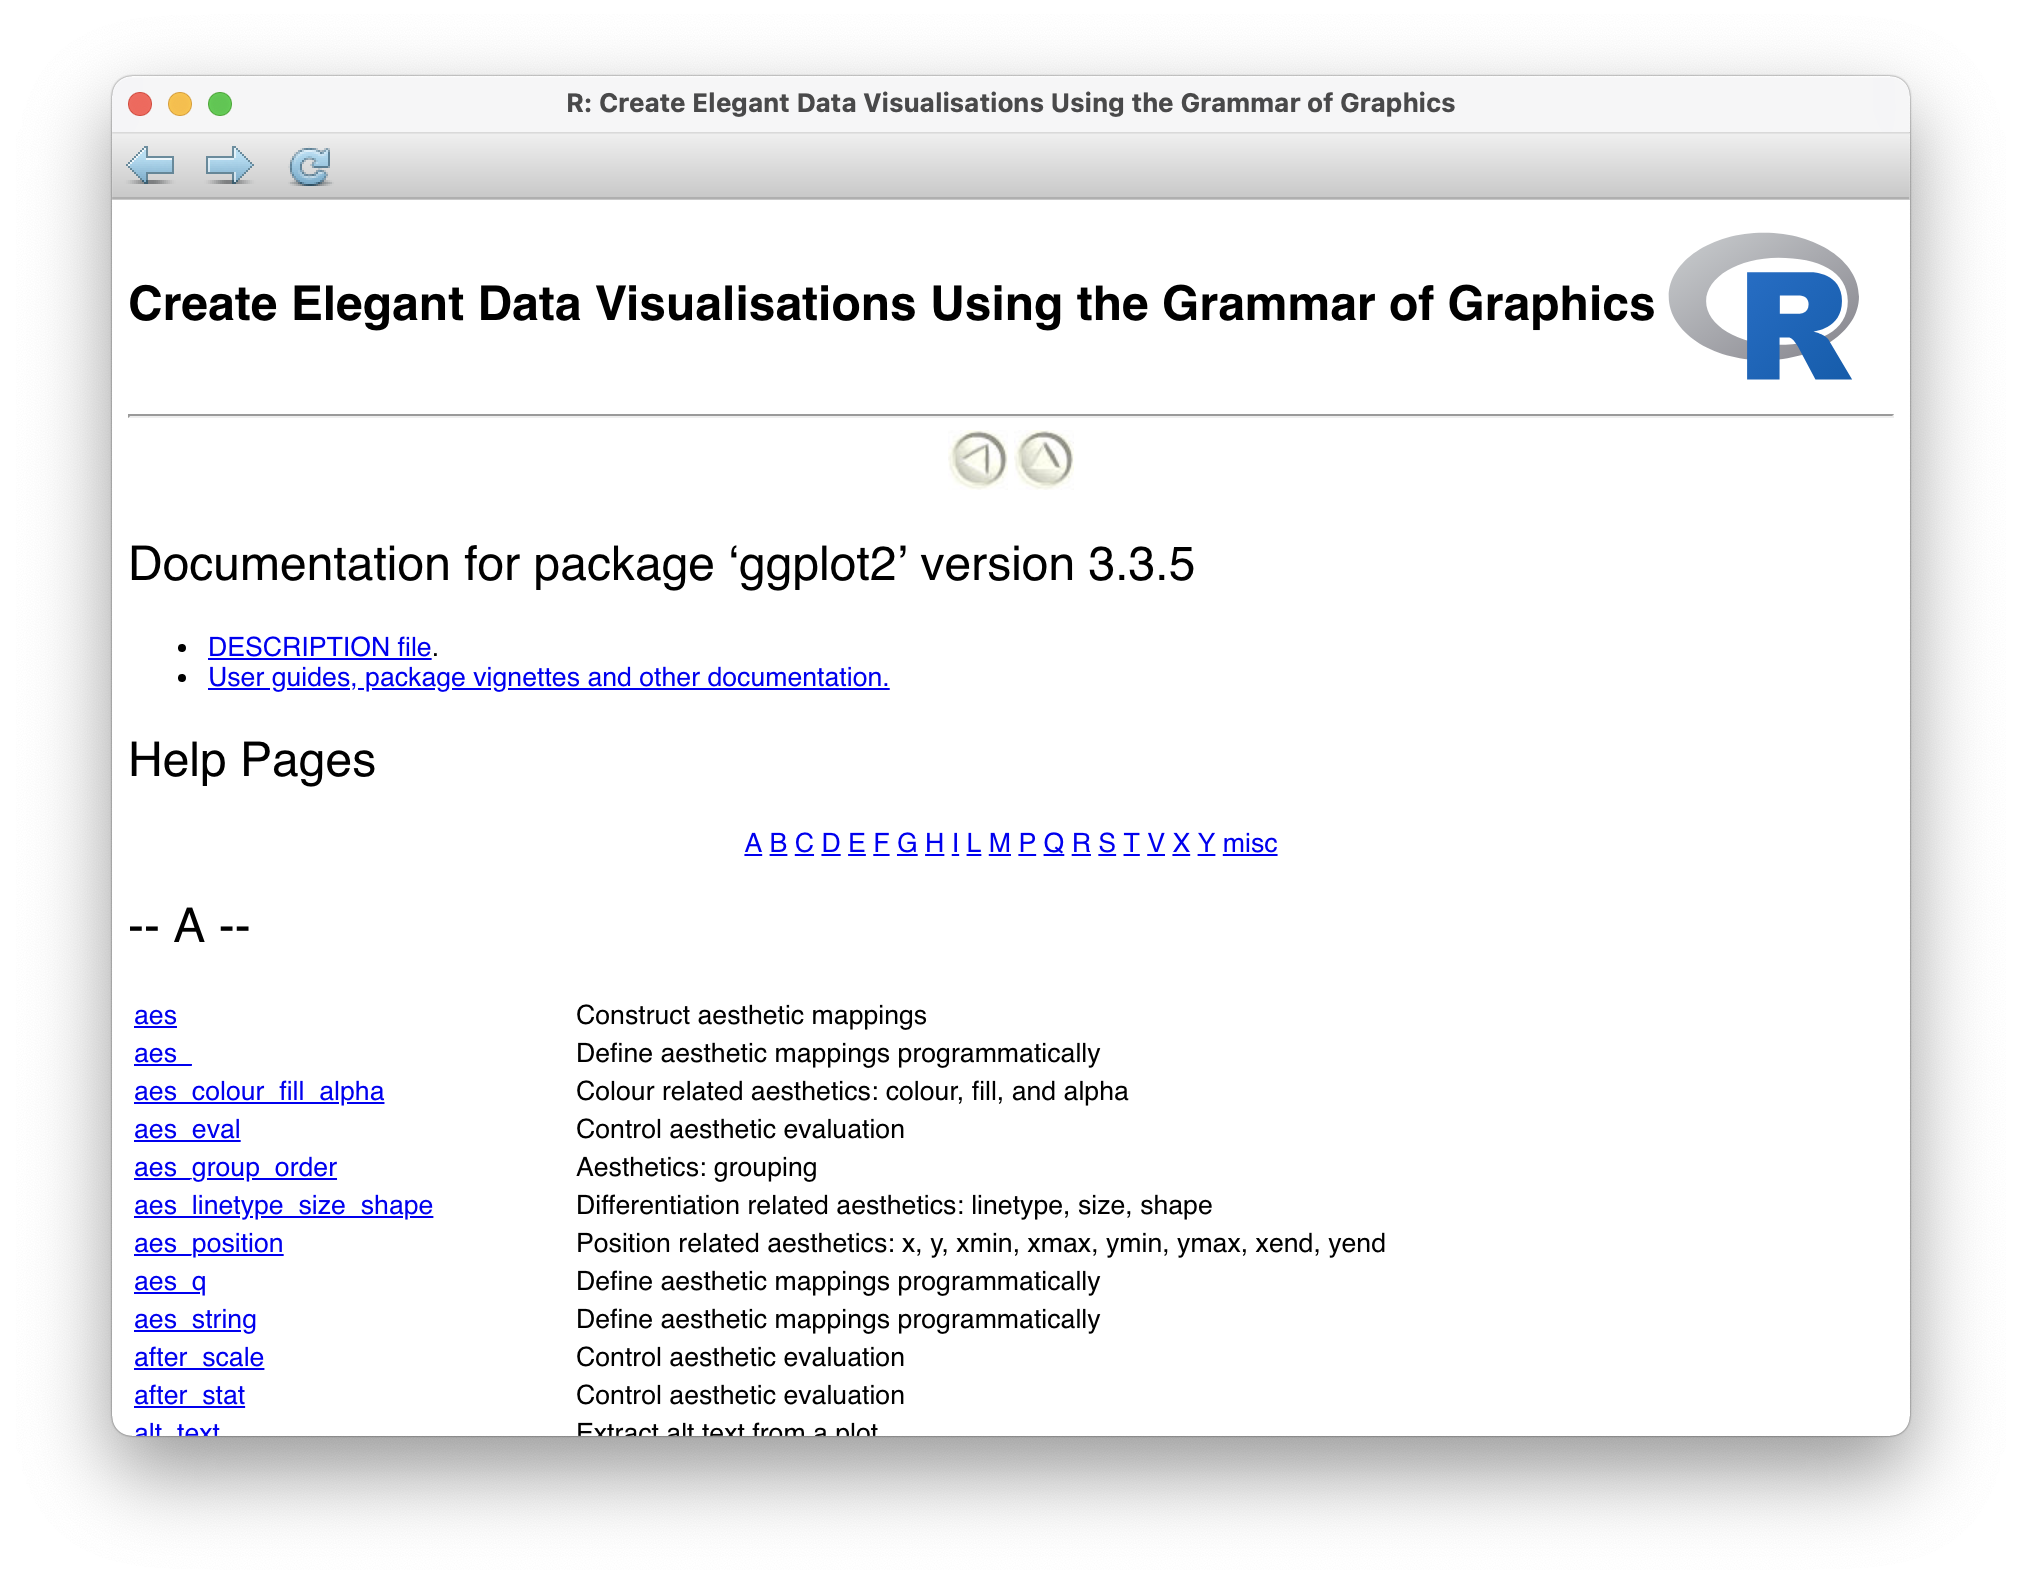
\includegraphics{images/chapter_05_img/r_package_documentation.png}

}

\caption{\label{fig-img-r-package-documentation}The R package
documentation for `ggplot2'}

\end{figure}%

However, how do you find those \emph{R} packages? They are right at your
fingertips. You have two options:

\begin{enumerate}
\def\labelenumi{\arabic{enumi}.}
\item
  Use the function \texttt{install.packages()}, or
\item
  Use the packages pane in RStudio.
\end{enumerate}

\subsection{\texorpdfstring{Installing packages using
\texttt{install.packages()}}{Installing packages using install.packages()}}\label{sec-installing-packages-using-a-function}

The simplest and fastest way to install a package is calling the
function \texttt{install.packages()}. You can either use it to install a
single package or install a series of packages all at once using our
trusty \texttt{c()} function. All you need to know is the name of the
package. This approach works for all packages that are on CRAN (remember
CRAN from Section~\ref{sec-installing-r} ?).

\begin{Shaded}
\begin{Highlighting}[]
\CommentTok{\# Install a single package}
\FunctionTok{install.packages}\NormalTok{(}\StringTok{"tidyverse"}\NormalTok{)}

\CommentTok{\# Install multiple packages at once}
\FunctionTok{install.packages}\NormalTok{(}\FunctionTok{c}\NormalTok{(}\StringTok{"tidyverse"}\NormalTok{, }\StringTok{"naniar"}\NormalTok{, }\StringTok{"psych"}\NormalTok{))}
\end{Highlighting}
\end{Shaded}

If a package is not available from CRAN, chances are you can find them
on \href{https://github.com}{GitHub}. GitHub is probably the world's
largest global platform for programmers from all walks of life, and many
of them develop fantastic \emph{R} packages that make programming and
data analysis not just easier but a lot more fun. As you continue to
work in \emph{R}, you should seriously consider creating your own
account to keep backups of your projects (see also
Section~\ref{sec-next-steps-github}).

An essential companion for this book is \texttt{r4np}, which contains
all datasets for this book and some useful functions to get you up and
running in no time. Since it is currently only available on Github, you
can use the following code snippet to install it. However, you have to
install the package \texttt{devtools} first to use the function
\texttt{install\_github()}.

\begin{Shaded}
\begin{Highlighting}[]
\CommentTok{\# Install the \textquotesingle{}devtools\textquotesingle{} package first}
\FunctionTok{install.packages}\NormalTok{(}\StringTok{"devtools"}\NormalTok{)}

\CommentTok{\# Then install the \textquotesingle{}r4np\textquotesingle{} package from GitHub}
\NormalTok{devtools}\SpecialCharTok{::}\FunctionTok{install\_github}\NormalTok{(}\StringTok{"ddauber/r4np"}\NormalTok{)}
\end{Highlighting}
\end{Shaded}

\subsection{Installing packages via RStudio's package
pane}\label{sec-installing-packages-via-rstudio}

RStudio offers a very convenient way of installing packages. In the
packages pane, you cannot only see your installed packages, but you have
two more buttons: \texttt{Install} and \texttt{Update}. The names are
very self-explanatory. To install an \emph{R} package you can follow the
following steps:

\begin{enumerate}
\def\labelenumi{\arabic{enumi}.}
\item
  Click on \texttt{Install}.
\item
  In most cases, you want to make sure you have
  \texttt{Repository\ (CRAN)} selected.

  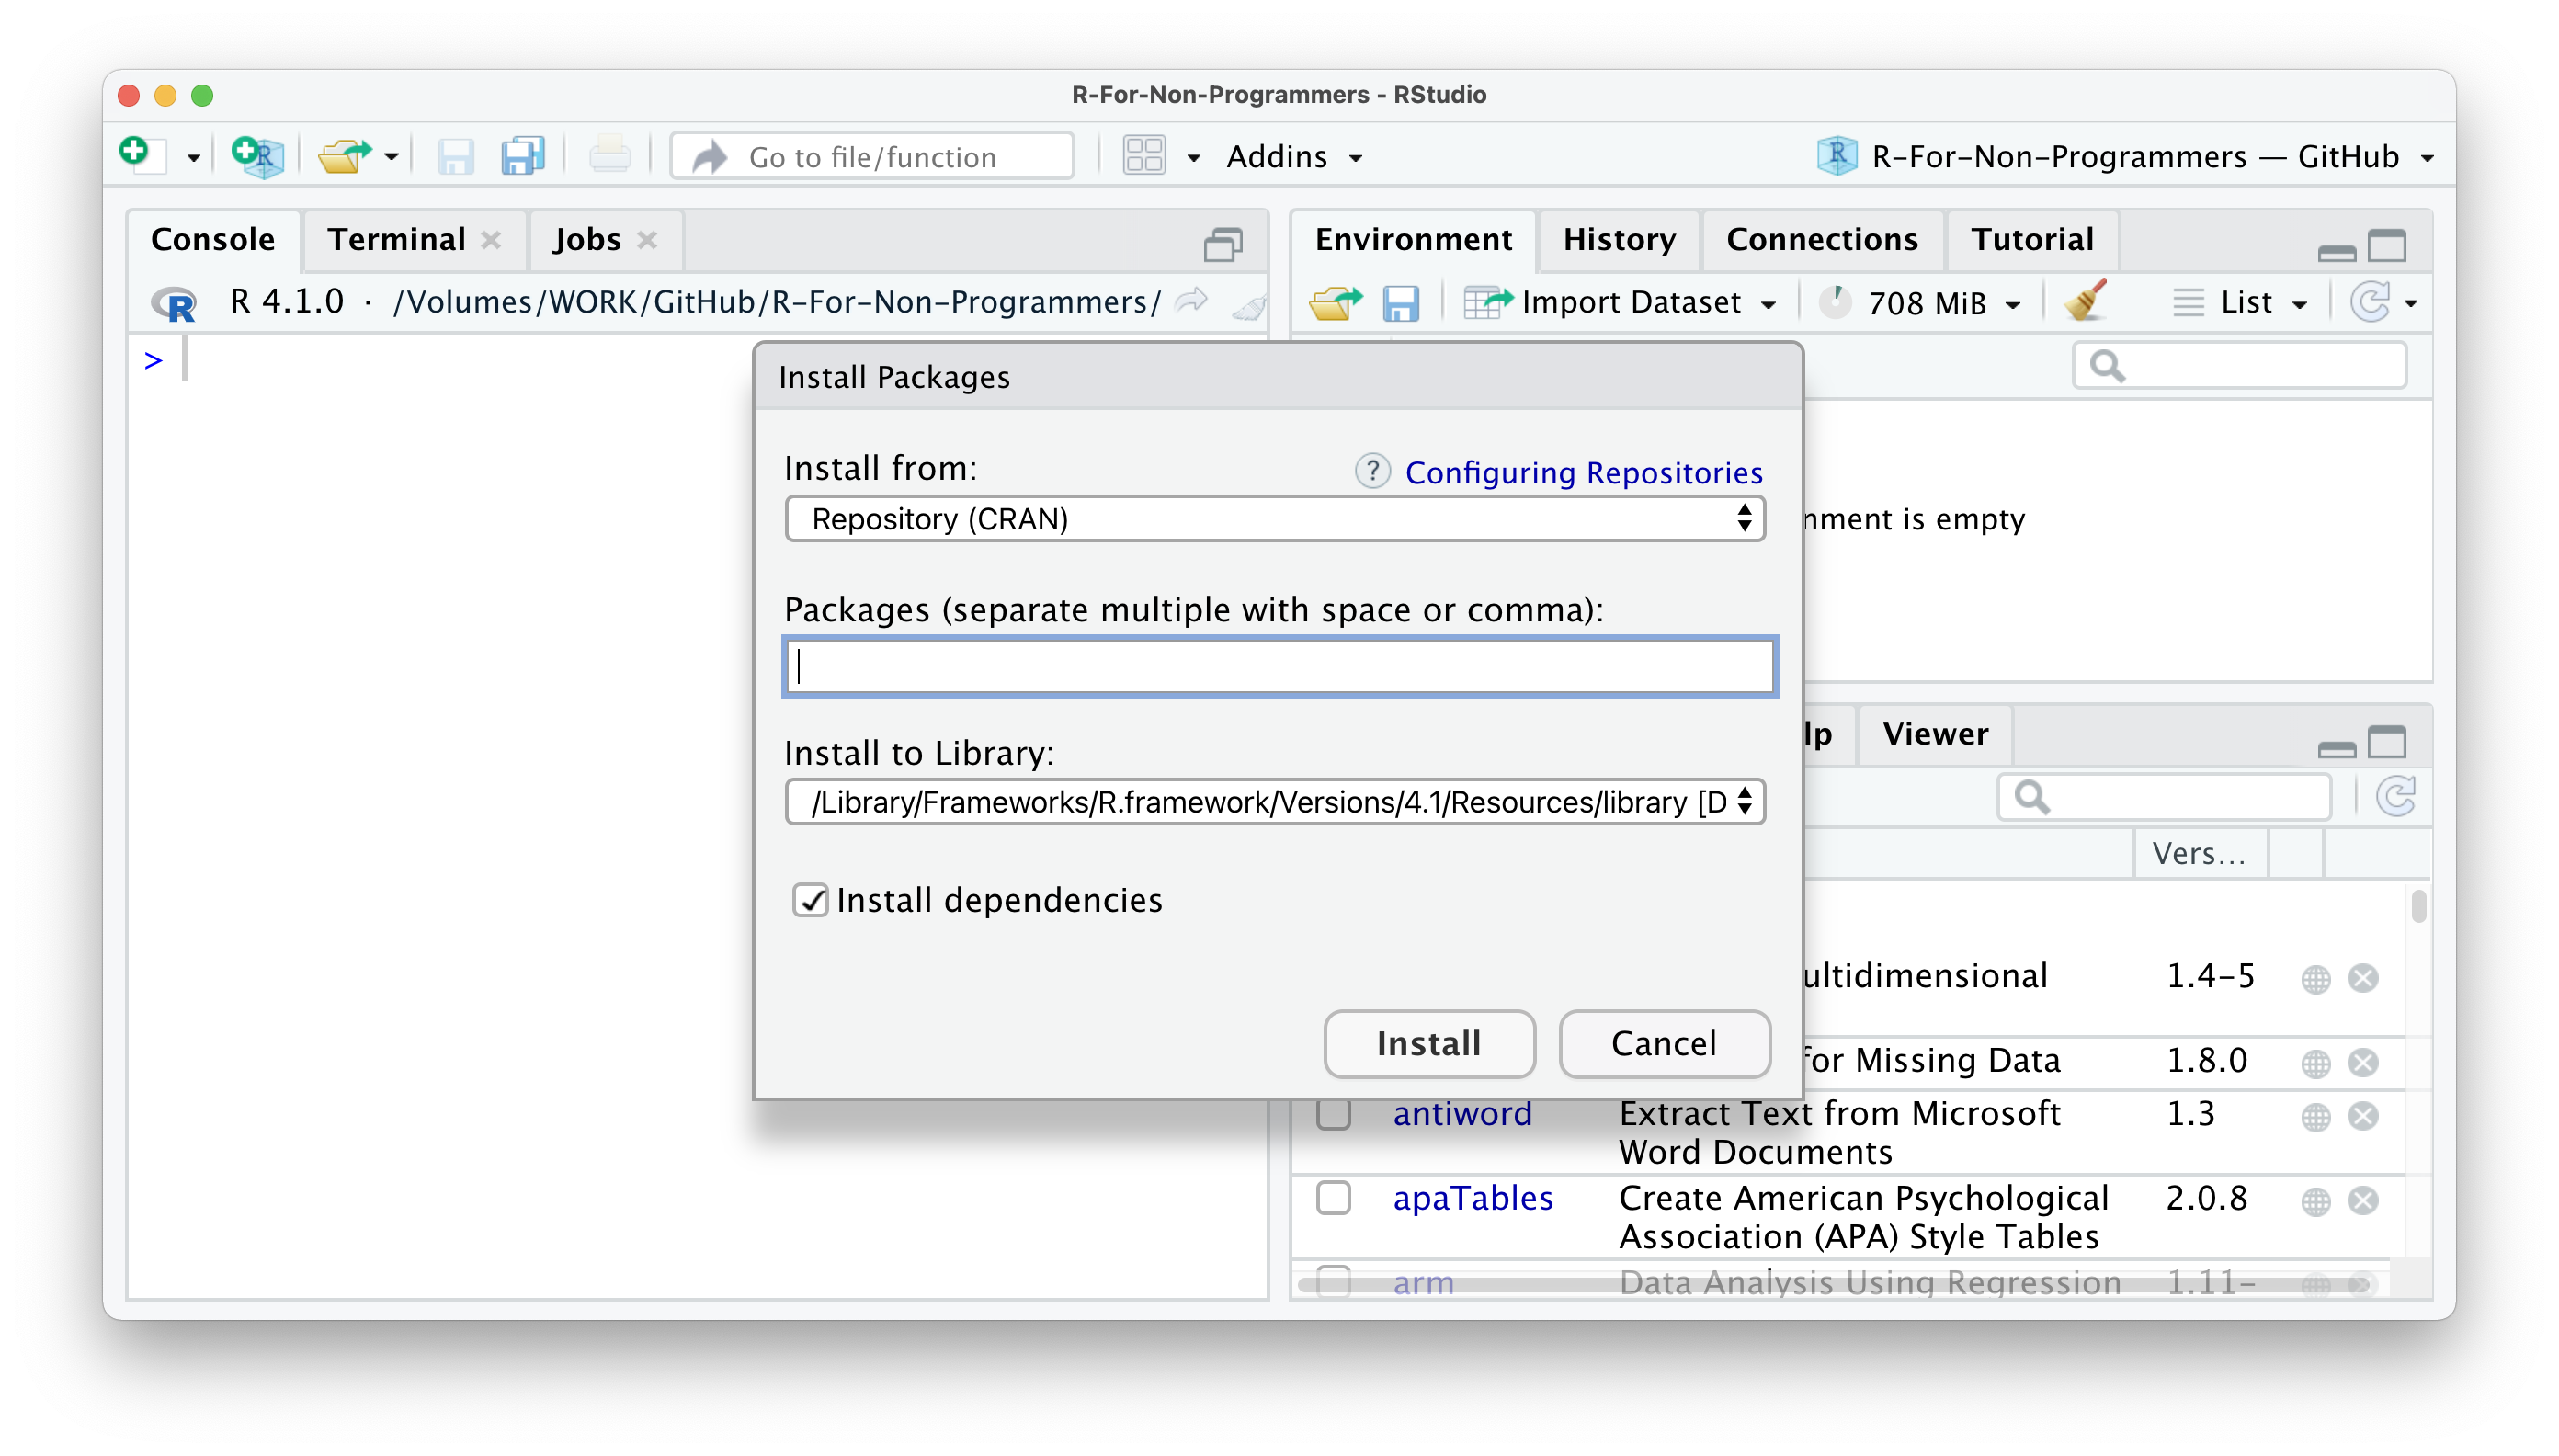
\includegraphics{images/chapter_05_img/install_r_packages/01_install_r_packages.png}
\item
  Type in the name of the package you wish to install. RStudio offers an
  auto-complete feature to make it even easier to find the package you
  want.

  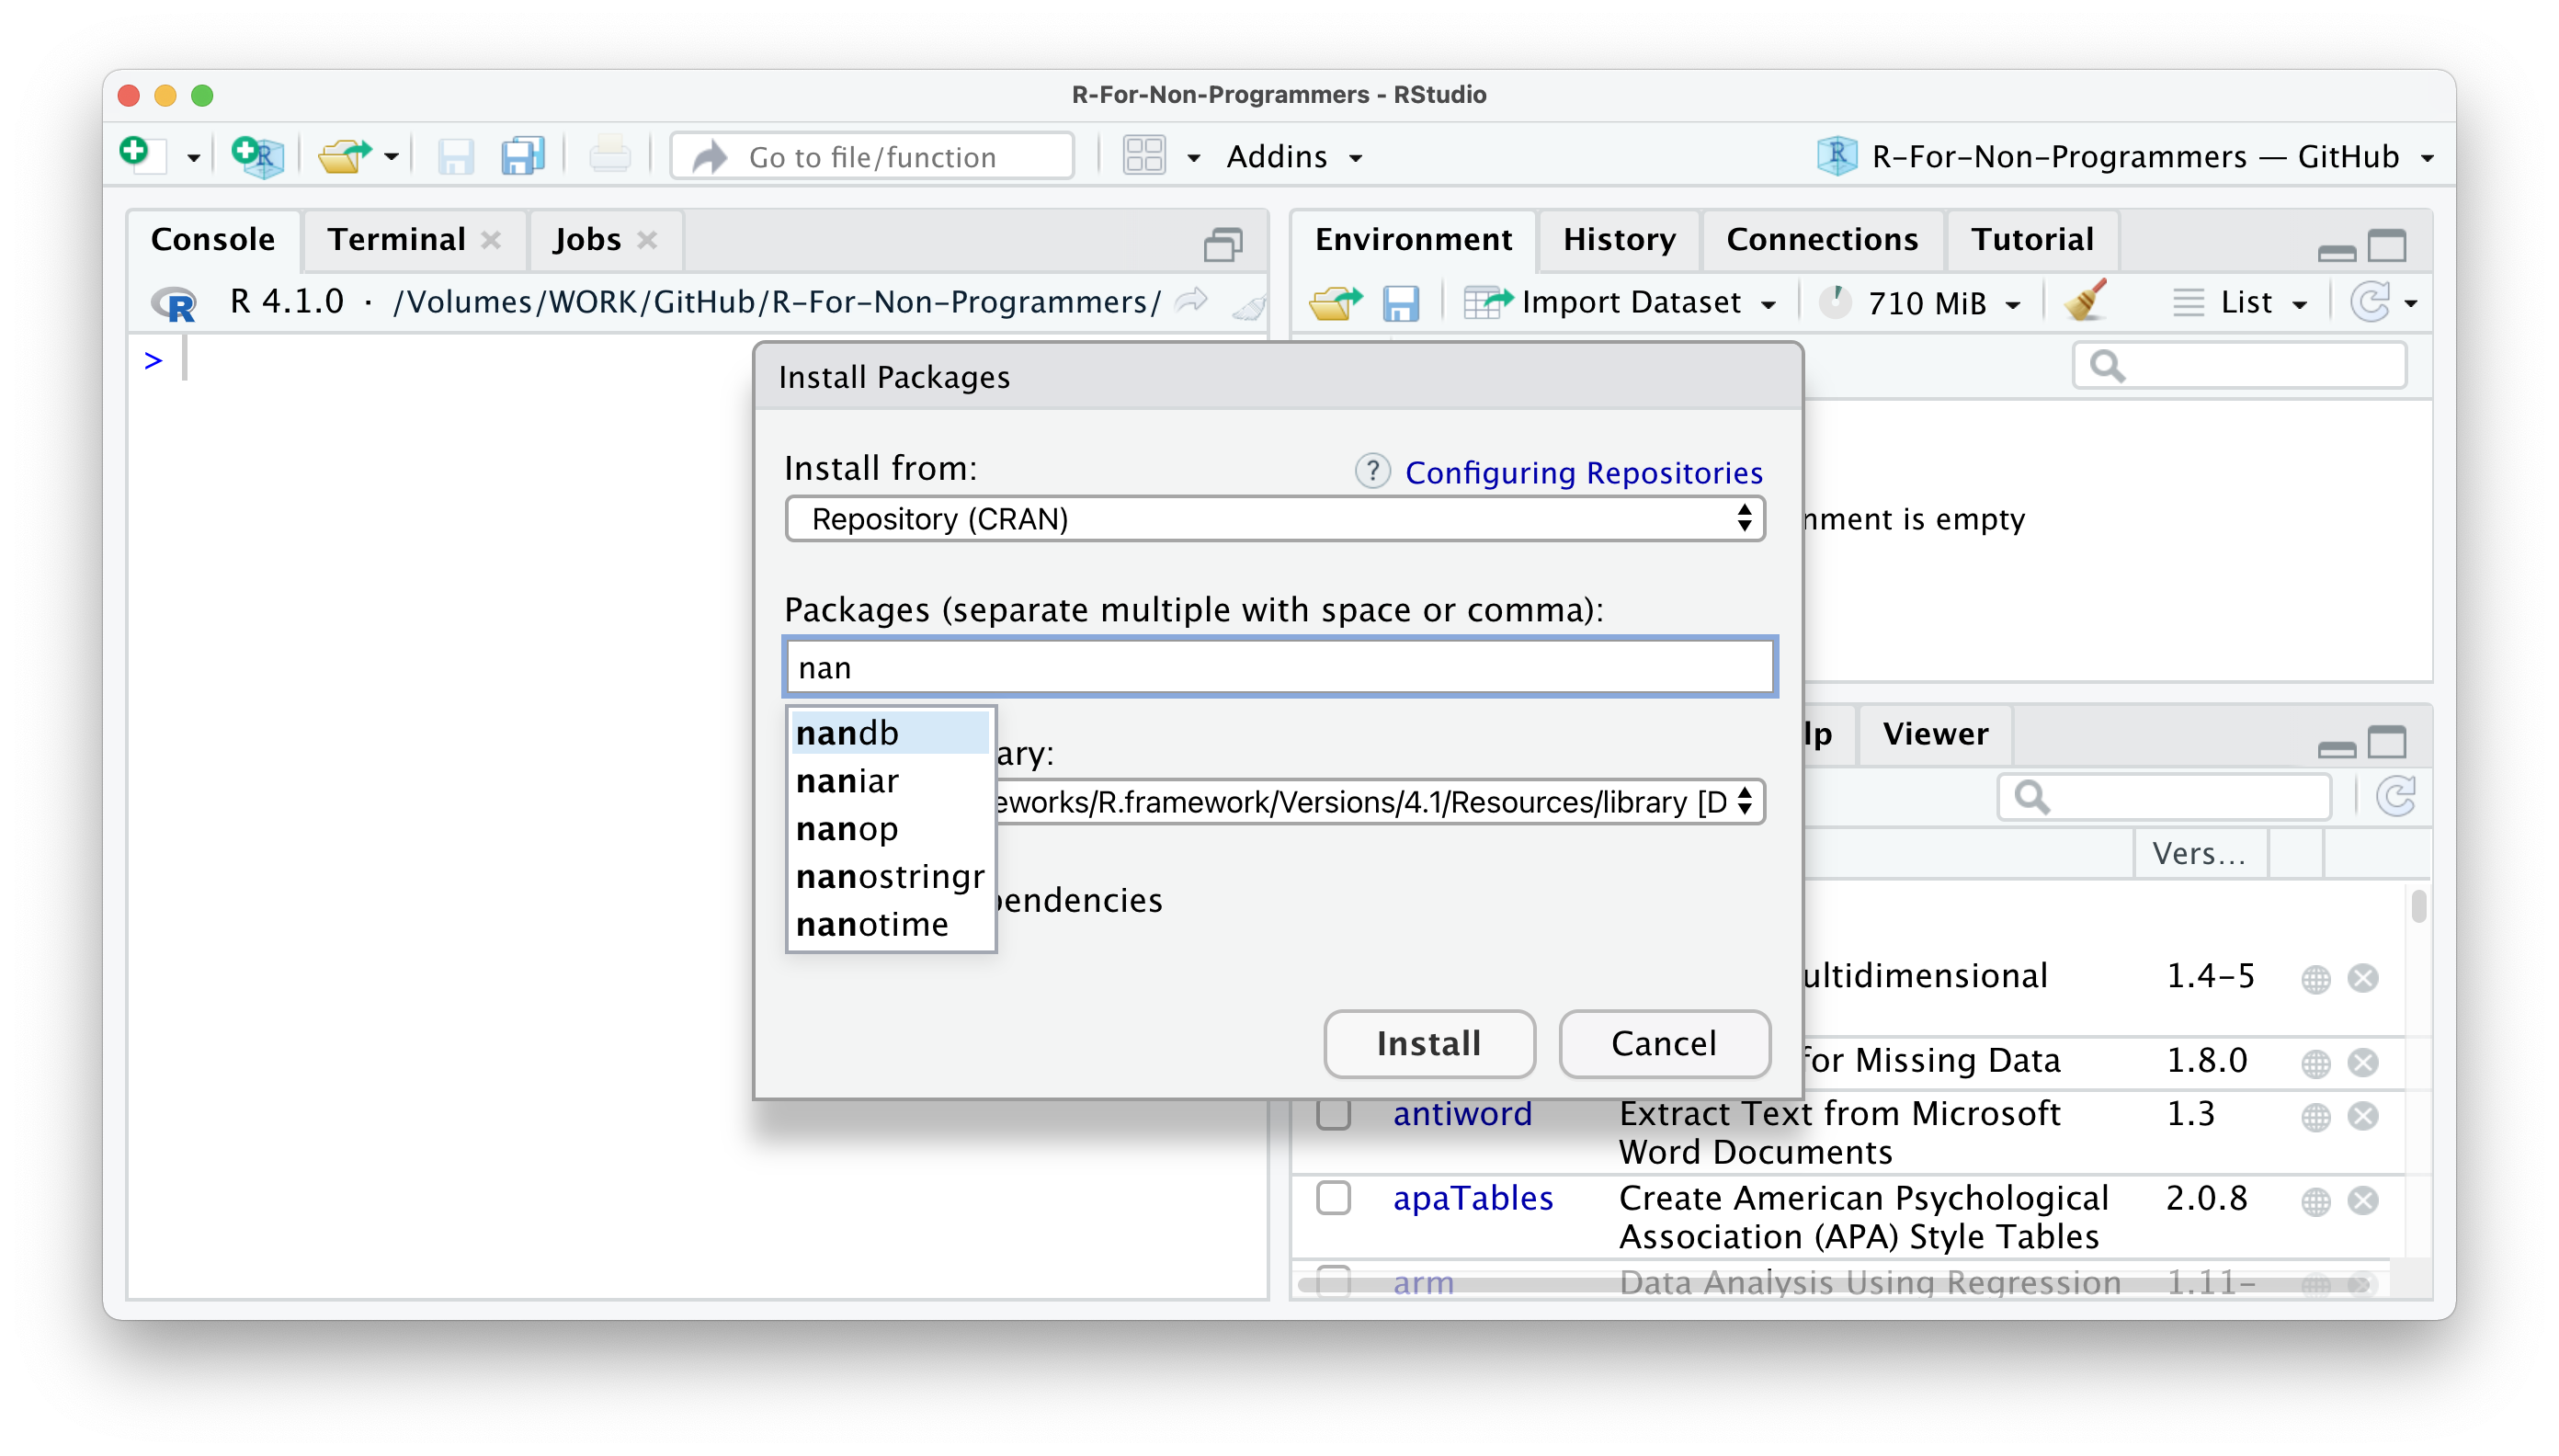
\includegraphics{images/chapter_05_img/install_r_packages/02_install_r_packages.png}
\item
  I recommend NOT to change the option which says
  \texttt{Install\ to\ library}. The default library settings will
  suffice.
\item
  Finally, I recommend to select \texttt{Install\ dependencies}, because
  some packages need other packages to function properly. This way, you
  do not have to do this manually.

  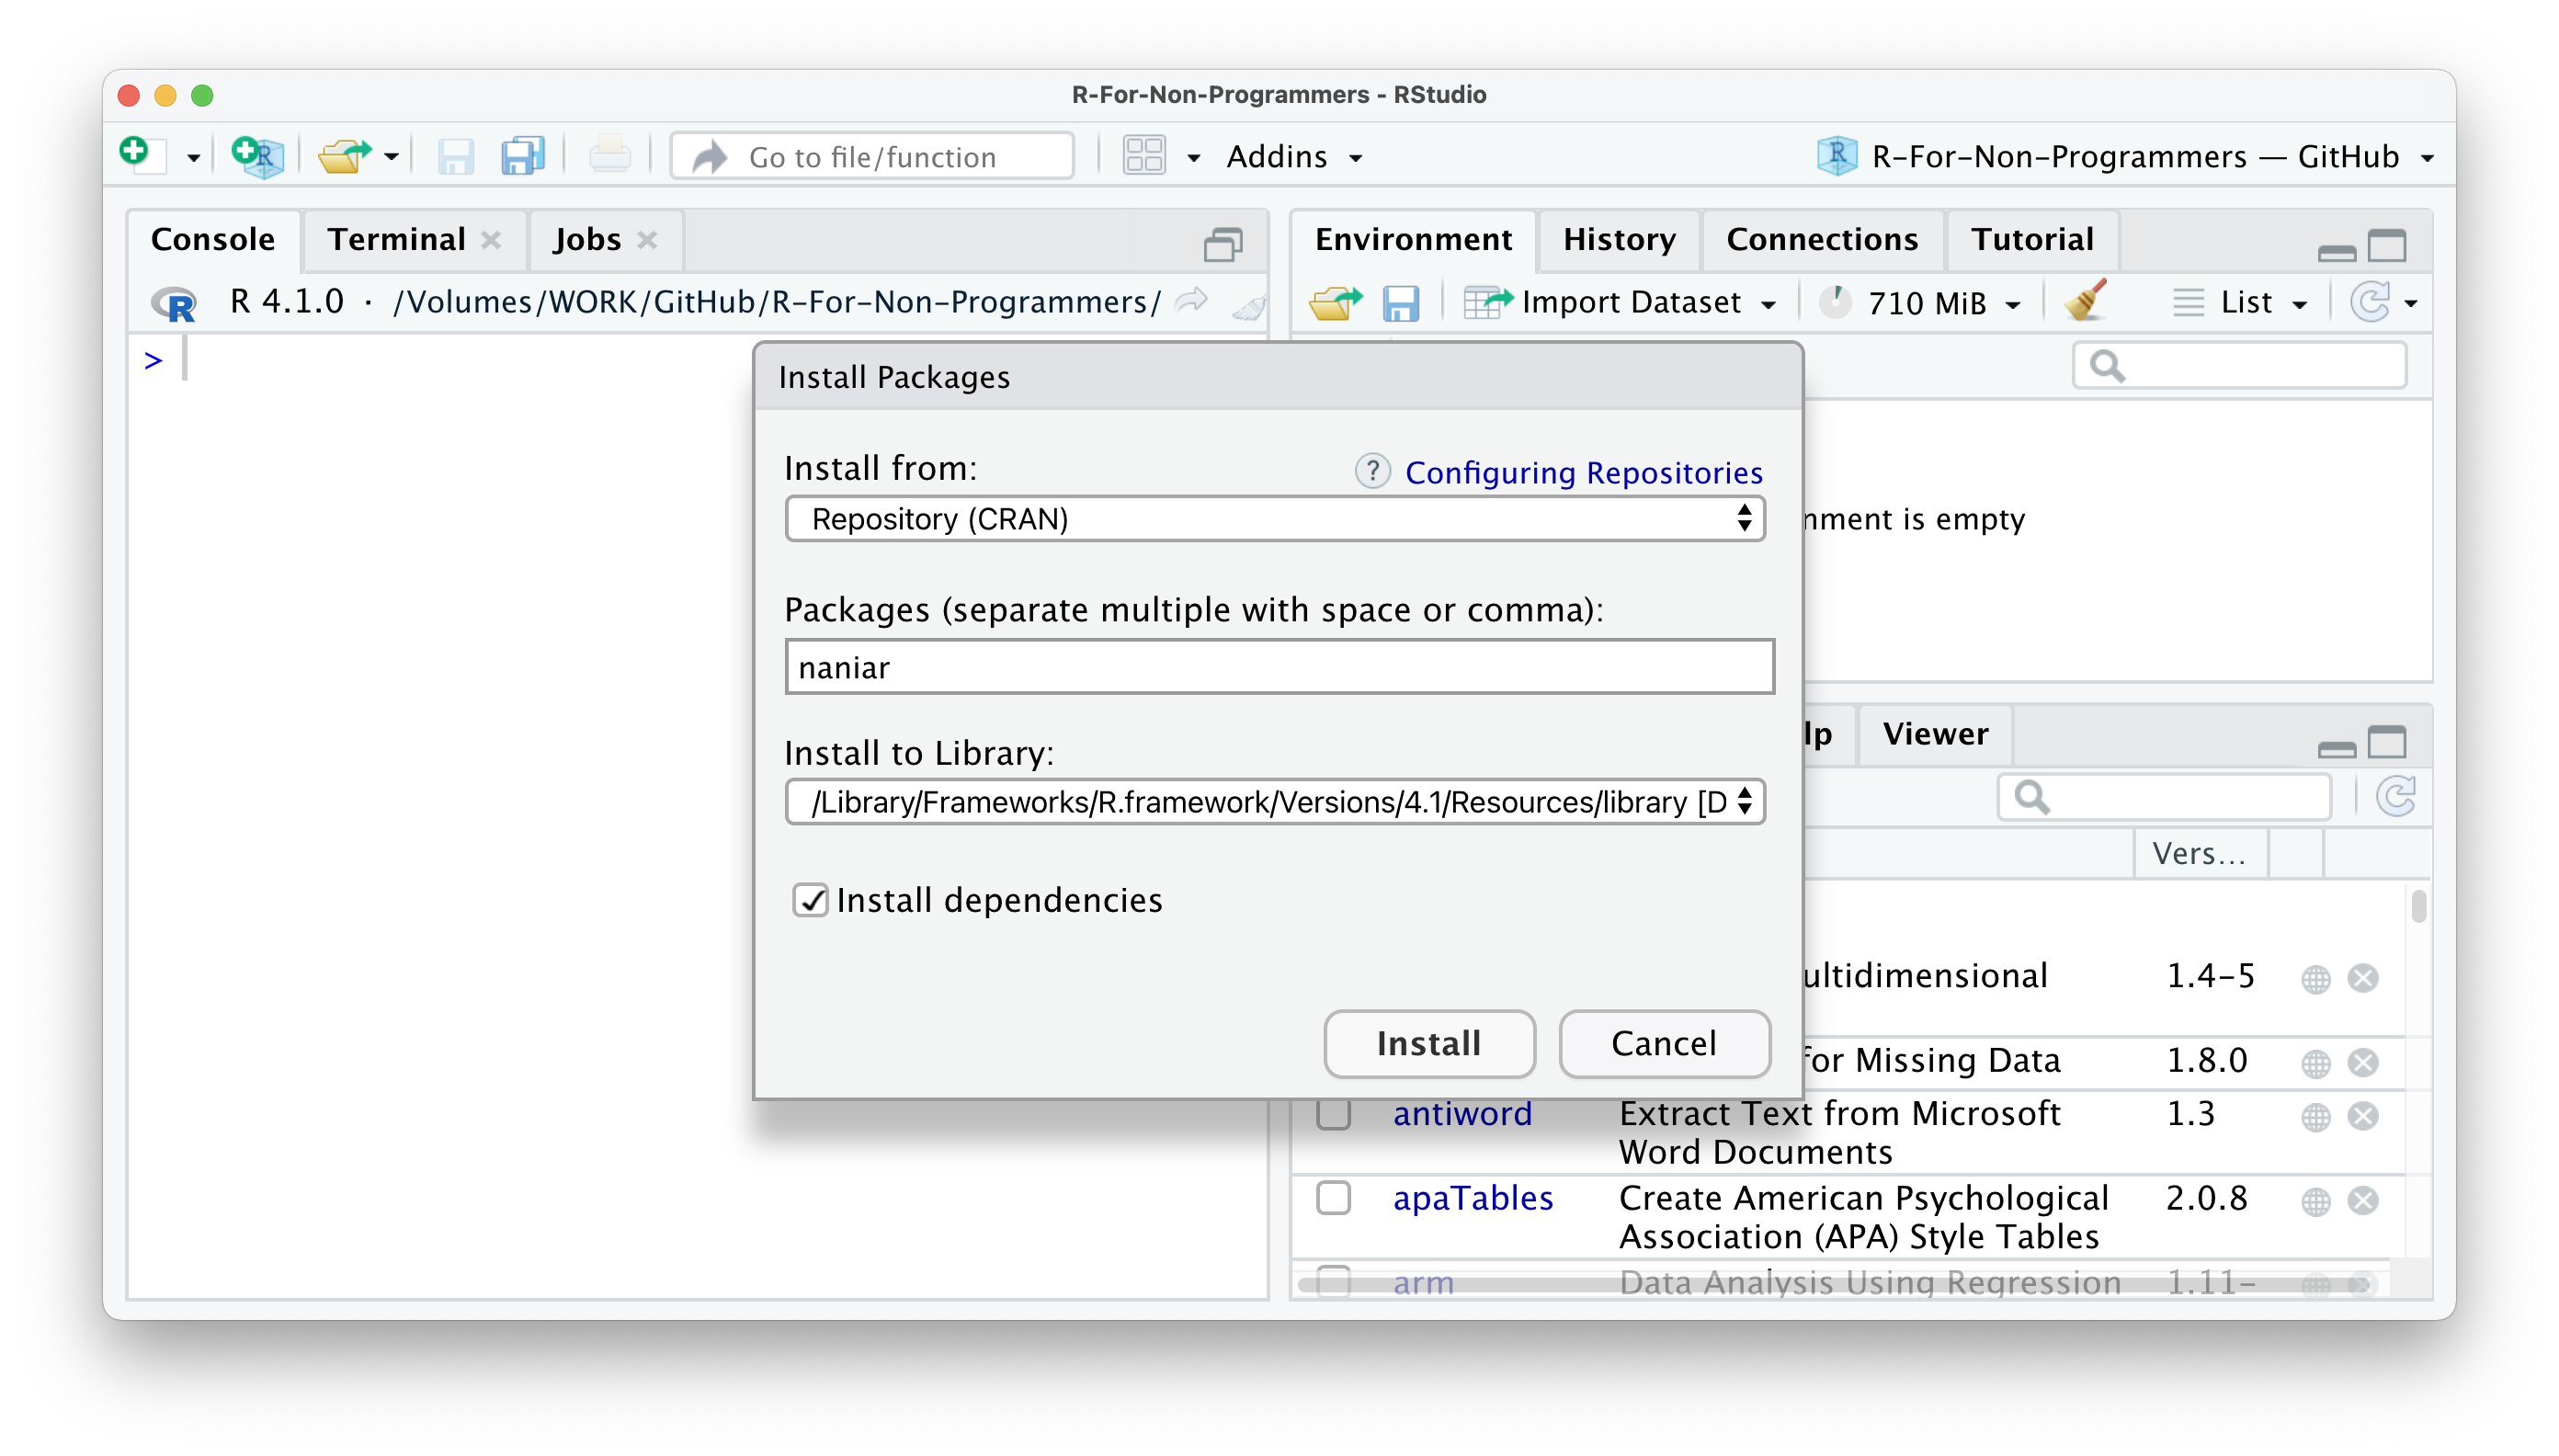
\includegraphics{images/chapter_05_img/install_r_packages/03_install_r_packages.png}
\end{enumerate}

The only real downside of using the packages pane is that you cannot
install packages hosted on GitHub only. However, you can download them
from there and install them directly from your computer using a this
option. This is particularly useful if you do not have an internet
connection but you already downloaded the required packages onto a hard
drive. However, in 99.9\% of cases it is much easier to use the function
\texttt{devtools::install\_github()} because you do not have to perform
multiple steps to achieve the same result.

\subsection{\texorpdfstring{Install all necessary \emph{R} packages for
this
book}{Install all necessary R packages for this book}}\label{sec-install-all-r-packages}

Lastly, if you would like to install the necessary packages to follow
the examples in this book, the \texttt{r4np} package comes with a handy
function to install them all at once. Of course, you need to have
\texttt{r4np} installed first, as shown \hyperref[install-r4np]{above}.

\begin{Shaded}
\begin{Highlighting}[]
\CommentTok{\# Install all R packages used in this book}
\NormalTok{r4np}\SpecialCharTok{::}\FunctionTok{install\_r4np}\NormalTok{()}
\end{Highlighting}
\end{Shaded}

\subsection{\texorpdfstring{Using \emph{R}
Packages}{Using R Packages}}\label{sec-using-r-packages}

Now that you have a nice collection of \emph{R} packages, the next step
would be to use them. While you only have to install \emph{R} packages
once, you have to `activate' them every time you start a new session in
RStudio. This process is also called `loading an \emph{R} package'. Once
an \emph{R} package is loaded, you can use all its functions. To load an
\emph{R} package, we have to use the function \texttt{library()}.

\begin{Shaded}
\begin{Highlighting}[]
\FunctionTok{library}\NormalTok{(tidyverse)}
\end{Highlighting}
\end{Shaded}

The \texttt{tidyverse} package is a special kind of package. It contains
multiple packages and loads them all at once. Almost all included
packages you will use at some point when working through this book.

I know what you are thinking. Can you use \texttt{c()} to load all your
packages at once? Unfortunately not. However, there is a way to do this,
but it goes beyond the scope of this book to fully explain this. If you
are curious, you can take a peek at the code
\href{https://stackoverflow.com/questions/8175912/load-multiple-packages-at-once}{here
on stackoverflow.com}.

Besides, it is not always advisable to load all functions of an entire
package. One reason could be that two packages contain a function with
the same name but with a different purpose. Two functions with the same
name create a conflict between these two packages, and one of the
functions would not be usable. Another reason could be that you only
need to use the function once, and loading the whole package to use only
one specific function seems excessive. Instead, you can explicitly call
functions from packages without loading the package. For example, we
might want to use the \texttt{vis\_miss()} function from the
\texttt{naniar} package to show where data is missing in our dataset
\texttt{airquality}. Using functions without \texttt{library()} is also
much quicker than loading the package and then calling the function if
you don't use it repeatedly. Make sure you have \texttt{naniar}
installed (see
\hyperref[install-packages-tidyverse-nanair-psych]{above}). We will work
with this package when we explore missing data in
Section~\ref{sec-dealing-with-missing-data} . To use a function from an
\emph{R} package without loading it, we have to use \texttt{::} between
the package's name and the function we want to use. Copy the code below
and try it yourself.

\begin{Shaded}
\begin{Highlighting}[]
\CommentTok{\# Here I use the dataset \textquotesingle{}airquality\textquotesingle{}, which comes with R}
\NormalTok{naniar}\SpecialCharTok{::}\FunctionTok{vis\_miss}\NormalTok{(airquality)}
\end{Highlighting}
\end{Shaded}

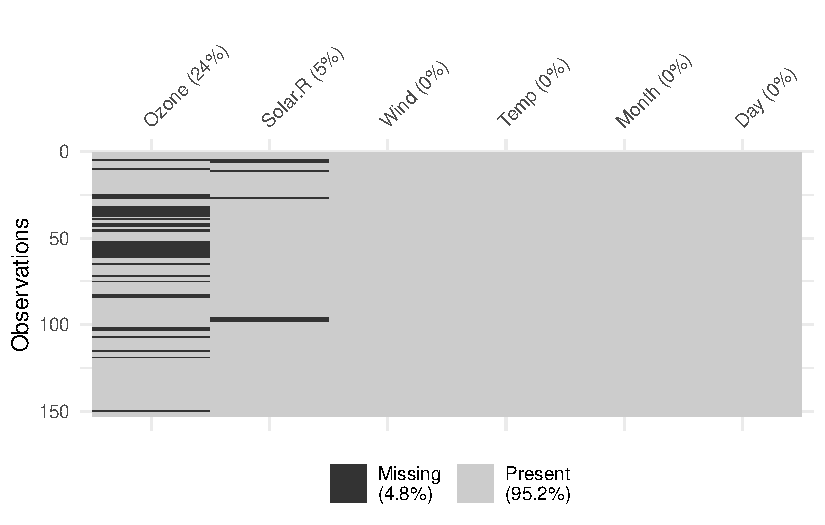
\includegraphics{05_r_basics_files/figure-latex/explicitly-calling-functions-1.pdf}

\section{Coding etiquette}\label{sec-coding-etiquette}

Now you know everything to get started, but before we jump into our
first project, I would like to briefly touch upon coding etiquette. This
is not something that improves your analytical or coding skills
directly, but is essential in building good habits and making your life
and those of others a little easier. Consider writing code like growing
plants in your garden. You want to nurture the good plants, remove the
weed and add labels that tell you which plant it is that you are
growing. At the end of the day, you want your garden to be
well-maintained. Treat you programming code the same way.

A script (see Section~\ref{sec-creating-an-r-script}) of programming
code should always have at least the following qualities:

\begin{itemize}
\item
  Only contains code that is necessary,
\item
  Is easy to read and understand,
\item
  Is self-contained.
\end{itemize}

With simple code this is easily achieved. However, what about more
complex and longer code representing a whole set of analytical steps?

\begin{Shaded}
\begin{Highlighting}[]
\CommentTok{\# Very messy code}

\FunctionTok{library}\NormalTok{(tidyverse)}
\FunctionTok{library}\NormalTok{(jtools)}
\NormalTok{model1 }\OtherTok{\textless{}{-}} \FunctionTok{lm}\NormalTok{(covid\_cases\_per\_1m }\SpecialCharTok{\textasciitilde{}}\NormalTok{ idv, }\AttributeTok{data =}\NormalTok{ df)}
\FunctionTok{summ}\NormalTok{(model1, }\AttributeTok{scale =} \ConstantTok{TRUE}\NormalTok{, }\AttributeTok{transform.response =} \ConstantTok{TRUE}\NormalTok{, }\AttributeTok{vifs =} \ConstantTok{TRUE}\NormalTok{)}
\NormalTok{df }\SpecialCharTok{|\textgreater{}} \FunctionTok{ggplot}\NormalTok{(}\FunctionTok{aes}\NormalTok{(}\AttributeTok{x =}\NormalTok{ covid\_cases\_per\_1m, }\AttributeTok{y =}\NormalTok{ idv, }\AttributeTok{col =}\NormalTok{ europe,}
                 \AttributeTok{label =}\NormalTok{ country))}\SpecialCharTok{+}
\FunctionTok{theme\_minimal}\NormalTok{()}\SpecialCharTok{+} \FunctionTok{geom\_label}\NormalTok{(}\AttributeTok{nudge\_y =} \DecValTok{2}\NormalTok{) }\SpecialCharTok{+} \FunctionTok{geom\_point}\NormalTok{()}
\NormalTok{model2 }\OtherTok{\textless{}{-}} \FunctionTok{lm}\NormalTok{(cases\_per\_1m }\SpecialCharTok{\textasciitilde{}}\NormalTok{ idv }\SpecialCharTok{+}\NormalTok{ uai }\SpecialCharTok{+}\NormalTok{ idv}\SpecialCharTok{*}\NormalTok{europe }\SpecialCharTok{+}\NormalTok{ uai}\SpecialCharTok{*}\NormalTok{europe,}
             \AttributeTok{data =}\NormalTok{ df)}
\FunctionTok{summ}\NormalTok{(model2, }\AttributeTok{scale =} \ConstantTok{TRUE}\NormalTok{, }\AttributeTok{transform.response =} \ConstantTok{TRUE}\NormalTok{, }\AttributeTok{vifs =} \ConstantTok{TRUE}\NormalTok{)}
\FunctionTok{anova}\NormalTok{(model1, model2)}
\end{Highlighting}
\end{Shaded}

How about the following in comparison?

\begin{Shaded}
\begin{Highlighting}[]
\CommentTok{\# Nicely structured code}

\CommentTok{\# Load required R packages}
\FunctionTok{library}\NormalTok{(tidyverse)}
\FunctionTok{library}\NormalTok{(jtools)}

\CommentTok{\# {-}{-}{-}{-} Modelling COVID{-}19 cases {-}{-}{-}{-}}

\DocumentationTok{\#\# Specify and run a regression}
\NormalTok{model1 }\OtherTok{\textless{}{-}} \FunctionTok{lm}\NormalTok{(covid\_cases\_per\_1m }\SpecialCharTok{\textasciitilde{}}\NormalTok{ idv, }\AttributeTok{data =}\NormalTok{ df)}

\DocumentationTok{\#\# Retrieve the summary statistics of model1}
\FunctionTok{summ}\NormalTok{(model1,}
     \AttributeTok{scale =} \ConstantTok{TRUE}\NormalTok{,}
     \AttributeTok{transform.response =} \ConstantTok{TRUE}\NormalTok{,}
     \AttributeTok{vifs =} \ConstantTok{TRUE}\NormalTok{)}

\CommentTok{\# Does is matter whether a country lies in Europe?}

\DocumentationTok{\#\# Visualise covid cases, idv and being a European country}
\NormalTok{df }\SpecialCharTok{|\textgreater{}}
  \FunctionTok{ggplot}\NormalTok{(}\FunctionTok{aes}\NormalTok{(}\AttributeTok{x =}\NormalTok{ covid\_cases\_per\_1m,}
             \AttributeTok{y =}\NormalTok{ idv,}
             \AttributeTok{col =}\NormalTok{ europe,}
             \AttributeTok{label =}\NormalTok{ country)) }\SpecialCharTok{+}
  \FunctionTok{theme\_minimal}\NormalTok{() }\SpecialCharTok{+}
  \FunctionTok{geom\_label}\NormalTok{(}\AttributeTok{nudge\_y =} \DecValTok{2}\NormalTok{) }\SpecialCharTok{+}
  \FunctionTok{geom\_point}\NormalTok{()}

\DocumentationTok{\#\# Specify and run a revised regression}
\NormalTok{model2 }\OtherTok{\textless{}{-}} \FunctionTok{lm}\NormalTok{(cases\_per\_1m }\SpecialCharTok{\textasciitilde{}}\NormalTok{ idv }\SpecialCharTok{+}\NormalTok{ uai }\SpecialCharTok{+}\NormalTok{ idv}\SpecialCharTok{*}\NormalTok{europe }\SpecialCharTok{+}\NormalTok{ uai}\SpecialCharTok{*}\NormalTok{europe,}
                 \AttributeTok{data =}\NormalTok{ df)}

\DocumentationTok{\#\# Retrieve the summary statistics of model2}
\FunctionTok{summ}\NormalTok{(model2,}
     \AttributeTok{scale =} \ConstantTok{TRUE}\NormalTok{,}
     \AttributeTok{transform.response =} \ConstantTok{TRUE}\NormalTok{,}
     \AttributeTok{vifs =} \ConstantTok{TRUE}\NormalTok{)}

\DocumentationTok{\#\# Test whether model2 is an improvement over model1}
\FunctionTok{anova}\NormalTok{(model1, model2)}
\end{Highlighting}
\end{Shaded}

I hope we can agree that the second example is much easier to read and
understand even though you probably do not understand most of it yet.
For once, I separated the different analytical steps from each other
like paragraphs in a report. Apart from that, I added comments with
\texttt{\#} to provide more context to my code for someone else who
wants to understand my analysis. Admittedly, this example is a little
excessive. Usually, you might have fewer comments. Commenting is an
integral part of programming because it allows you to remember what you
did or still have to do. Ideally, you want to strike a good balance
between commenting on and writing your code. How many comments you need
will likely change throughout your \emph{R} programming journey. Think
of comments as headers for your programming script that give it
structure.

We can use \texttt{\#} not only to write comments but also to tell
\emph{R} not to run particular code. This is very helpful if you want to
keep some code but do not want to use it yet. There is also a handy
keyboard shortcut you can use to `deactivate' multiple lines of code at
once. Select whatever you want to `comment out' in your script and press
\texttt{Ctrl+Shift+C} (PC) or \texttt{Cmd+Shift+C} (Mac).

\begin{Shaded}
\begin{Highlighting}[]
\CommentTok{\# mean(pocket\_money) \# R will NOT run this code}
\FunctionTok{mean}\NormalTok{(pocket\_money)   }\CommentTok{\# R will run this code}
\end{Highlighting}
\end{Shaded}

RStudio helps a lot with keeping your coding tidy and properly
formatted. However, there are some additional aspects worth considering.
If you want to find out more about coding style, I highly recommend to
read through \href{https://style.tidyverse.org}{\emph{`The tidyverse
style guide'}} (Wickham 2021).\\

\section{Exercises}\label{sec-exercises-r_basics}

It is time to practice the newly acquired skills. The \texttt{r4np}
package comes with interactive tutorials. In order to start them, you
have two options. If you have installed the \texttt{r4np} package
already and used the function \texttt{install\_r4np()} you can use
\texttt{Option\ 1}:

\begin{Shaded}
\begin{Highlighting}[]
\CommentTok{\# Option 1:}
\NormalTok{learnr}\SpecialCharTok{::}\FunctionTok{run\_tutorial}\NormalTok{(}\StringTok{"ex\_r\_basics"}\NormalTok{, }\AttributeTok{package =} \StringTok{"r4np"}\NormalTok{)}
\end{Highlighting}
\end{Shaded}

If you have not installed the \texttt{r4np} package and/or not run the
function \texttt{install\_r4np()}, you will have to do this first using
\texttt{Option\ 2}:

\begin{Shaded}
\begin{Highlighting}[]
\CommentTok{\# Option 2:}
\DocumentationTok{\#\# Install \textquotesingle{}r4np\textquotesingle{} package}
\NormalTok{devtools}\SpecialCharTok{::}\FunctionTok{install\_github}\NormalTok{(}\StringTok{"ddauber/r4np"}\NormalTok{)}

\DocumentationTok{\#\# Install all relevant packages for this book}
\NormalTok{r4np}\SpecialCharTok{::}\FunctionTok{install\_r4np}\NormalTok{()}

\DocumentationTok{\#\# Start the tutorial for this chapter}
\NormalTok{learnr}\SpecialCharTok{::}\FunctionTok{run\_tutorial}\NormalTok{(}\StringTok{"ex\_r\_basics"}\NormalTok{, }\AttributeTok{package =} \StringTok{"r4np"}\NormalTok{)}
\end{Highlighting}
\end{Shaded}

\bookmarksetup{startatroot}

\chapter{\texorpdfstring{Starting your \emph{R}
projects}{Starting your R projects}}\label{sec-starting-your-r-projects}

Every new project likely fills you with enthusiasm and excitement. And
it should. You are about to find answers to your research questions, and
you hopefully come out more knowledgeable because of it. However, you
likely find certain aspects of data analysis less enjoyable. I can think
of two:

\begin{itemize}
\item
  Keeping track of all the files my project generates
\item
  Data wrangling
\end{itemize}

While we cover data wrangling in great detail in the next Chapter
(Chapter~\ref{sec-data-wrangling}), I would like to share some insights
from my work that helped me stay organised and, consequently, less
frustrated. The following applies to small and large research projects,
which makes it very convenient no matter the situation and the scale of
the project. Of course, feel free to tweak my approach to whatever suits
you. However, consistency is king.

\section{\texorpdfstring{Creating an \emph{R} Project
file}{Creating an R Project file}}\label{sec-creating-an-r-project}

When working on a project, you likely create many different files for
various purposes, especially \emph{R} scripts (see
Section~\ref{sec-creating-an-r-project}). If you are not careful, this
file is stored in your system's default location, which might not be
where you want them to be. RStudio allows you to manage your entire
project intuitively and conveniently through \emph{R} Project files.
Using \emph{R} Project files comes with a couple of perks, for example:

\begin{itemize}
\item
  All the files that you generate are in the same place. Your data, your
  coding, your exported plots, your reports, etc., all are in one place
  together without you having to manage the files manually. This is due
  to the fact that RStudio sets the root directory to whichever folder
  your project is saved to.
\item
  If you want to share your project, you can share the entire folder,
  and others can quickly reproduce your research or help fix problems.
  This is because all file paths are relative and not absolute.
\item
  You can, more easily, use GitHub for backups and so-called `version
  control', which allows you to track changes you have made to your code
  over time (see also Section~\ref{sec-next-steps-github}).
\end{itemize}

For now, the most important reason to use \emph{R} Project files is the
convenience of the organisation of files and the ability to share it
easily with co-investigators, your supervisor, or your students.

To create an \emph{R} Project, you need to perform the following steps:

\begin{enumerate}
\def\labelenumi{\arabic{enumi}.}
\tightlist
\item
  Select \texttt{File\ \textgreater{}\ New\ Project…} from the menu bar.
\end{enumerate}

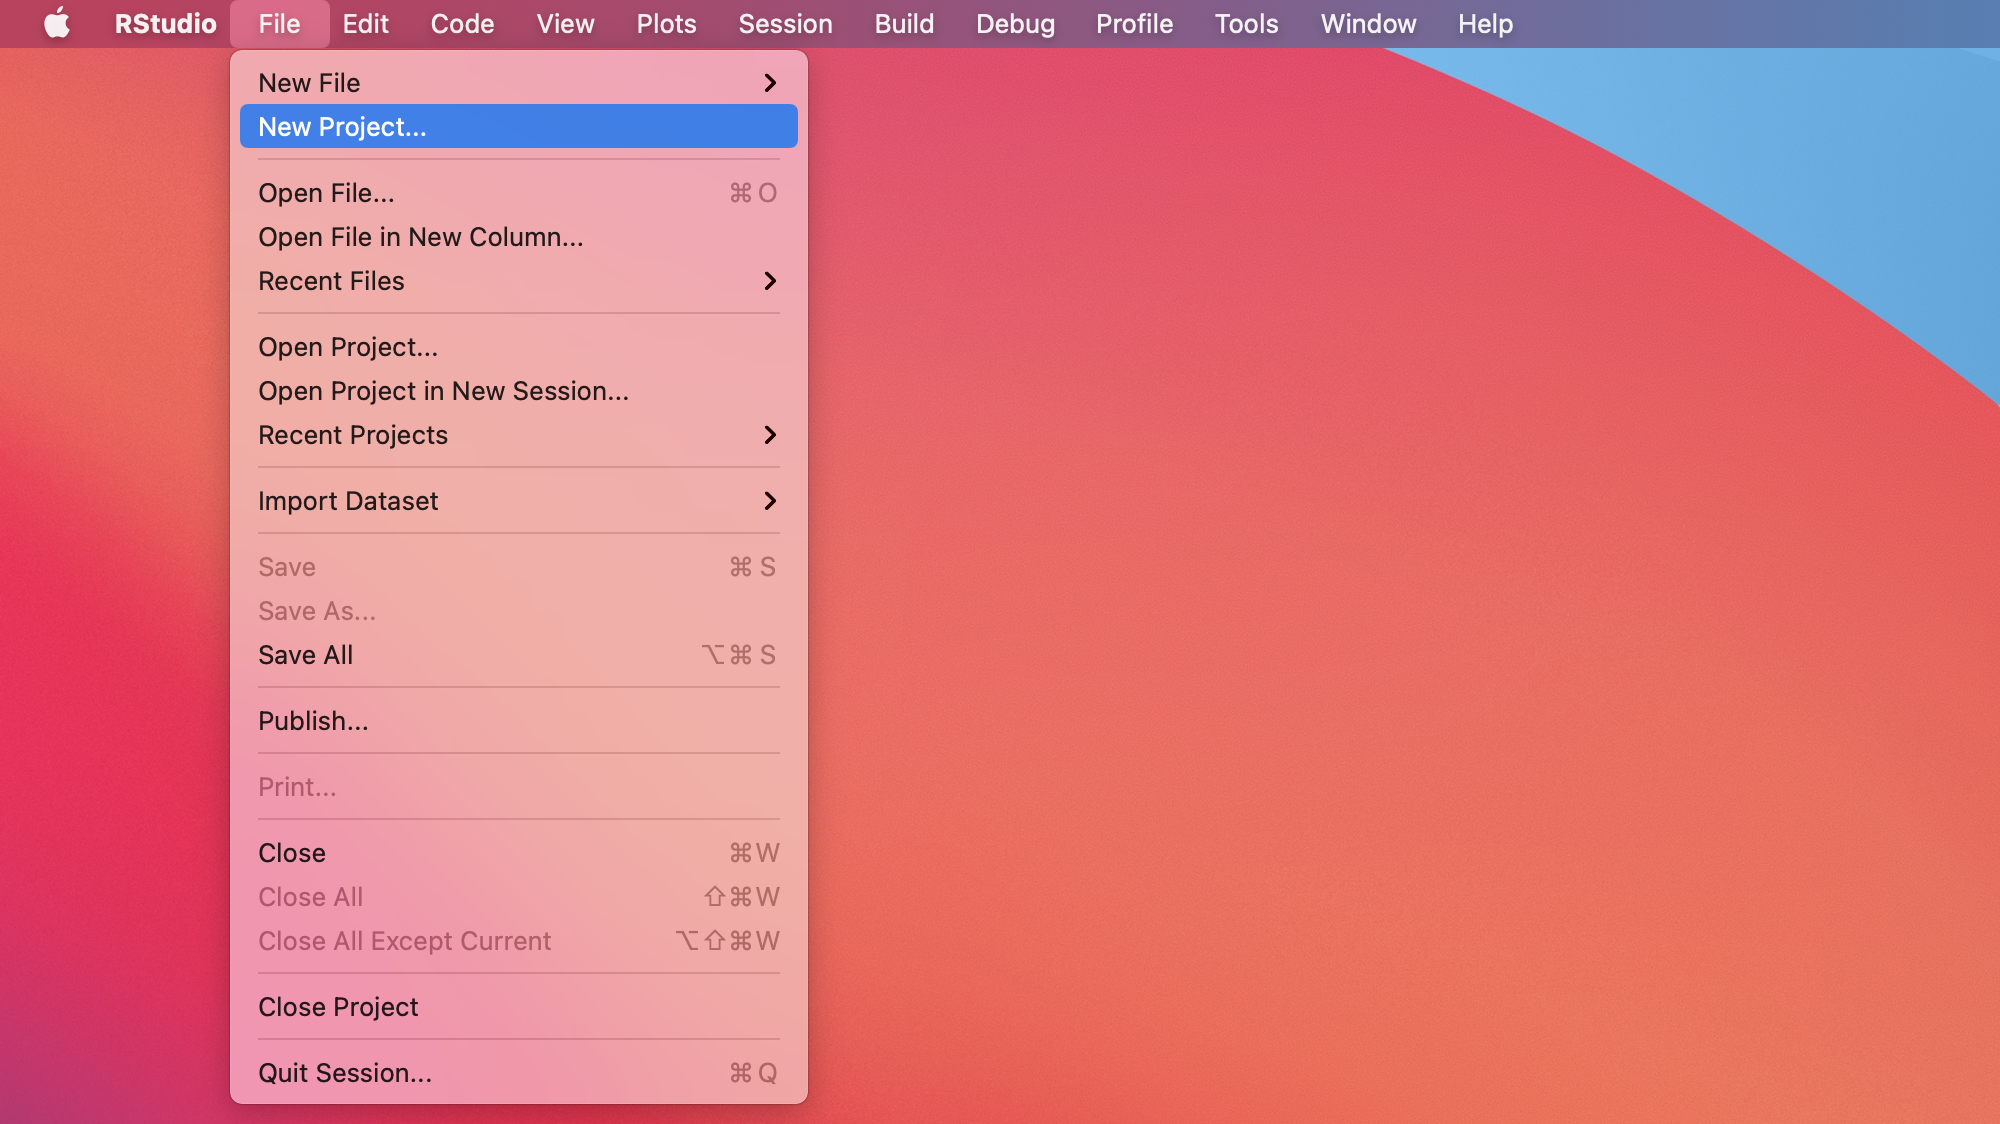
\includegraphics{images/chapter_06_img/00_r_project/00_r_project_file_menu.png}

\begin{enumerate}
\def\labelenumi{\arabic{enumi}.}
\setcounter{enumi}{1}
\tightlist
\item
  Select \texttt{New\ Directory} from the popup window.
\end{enumerate}

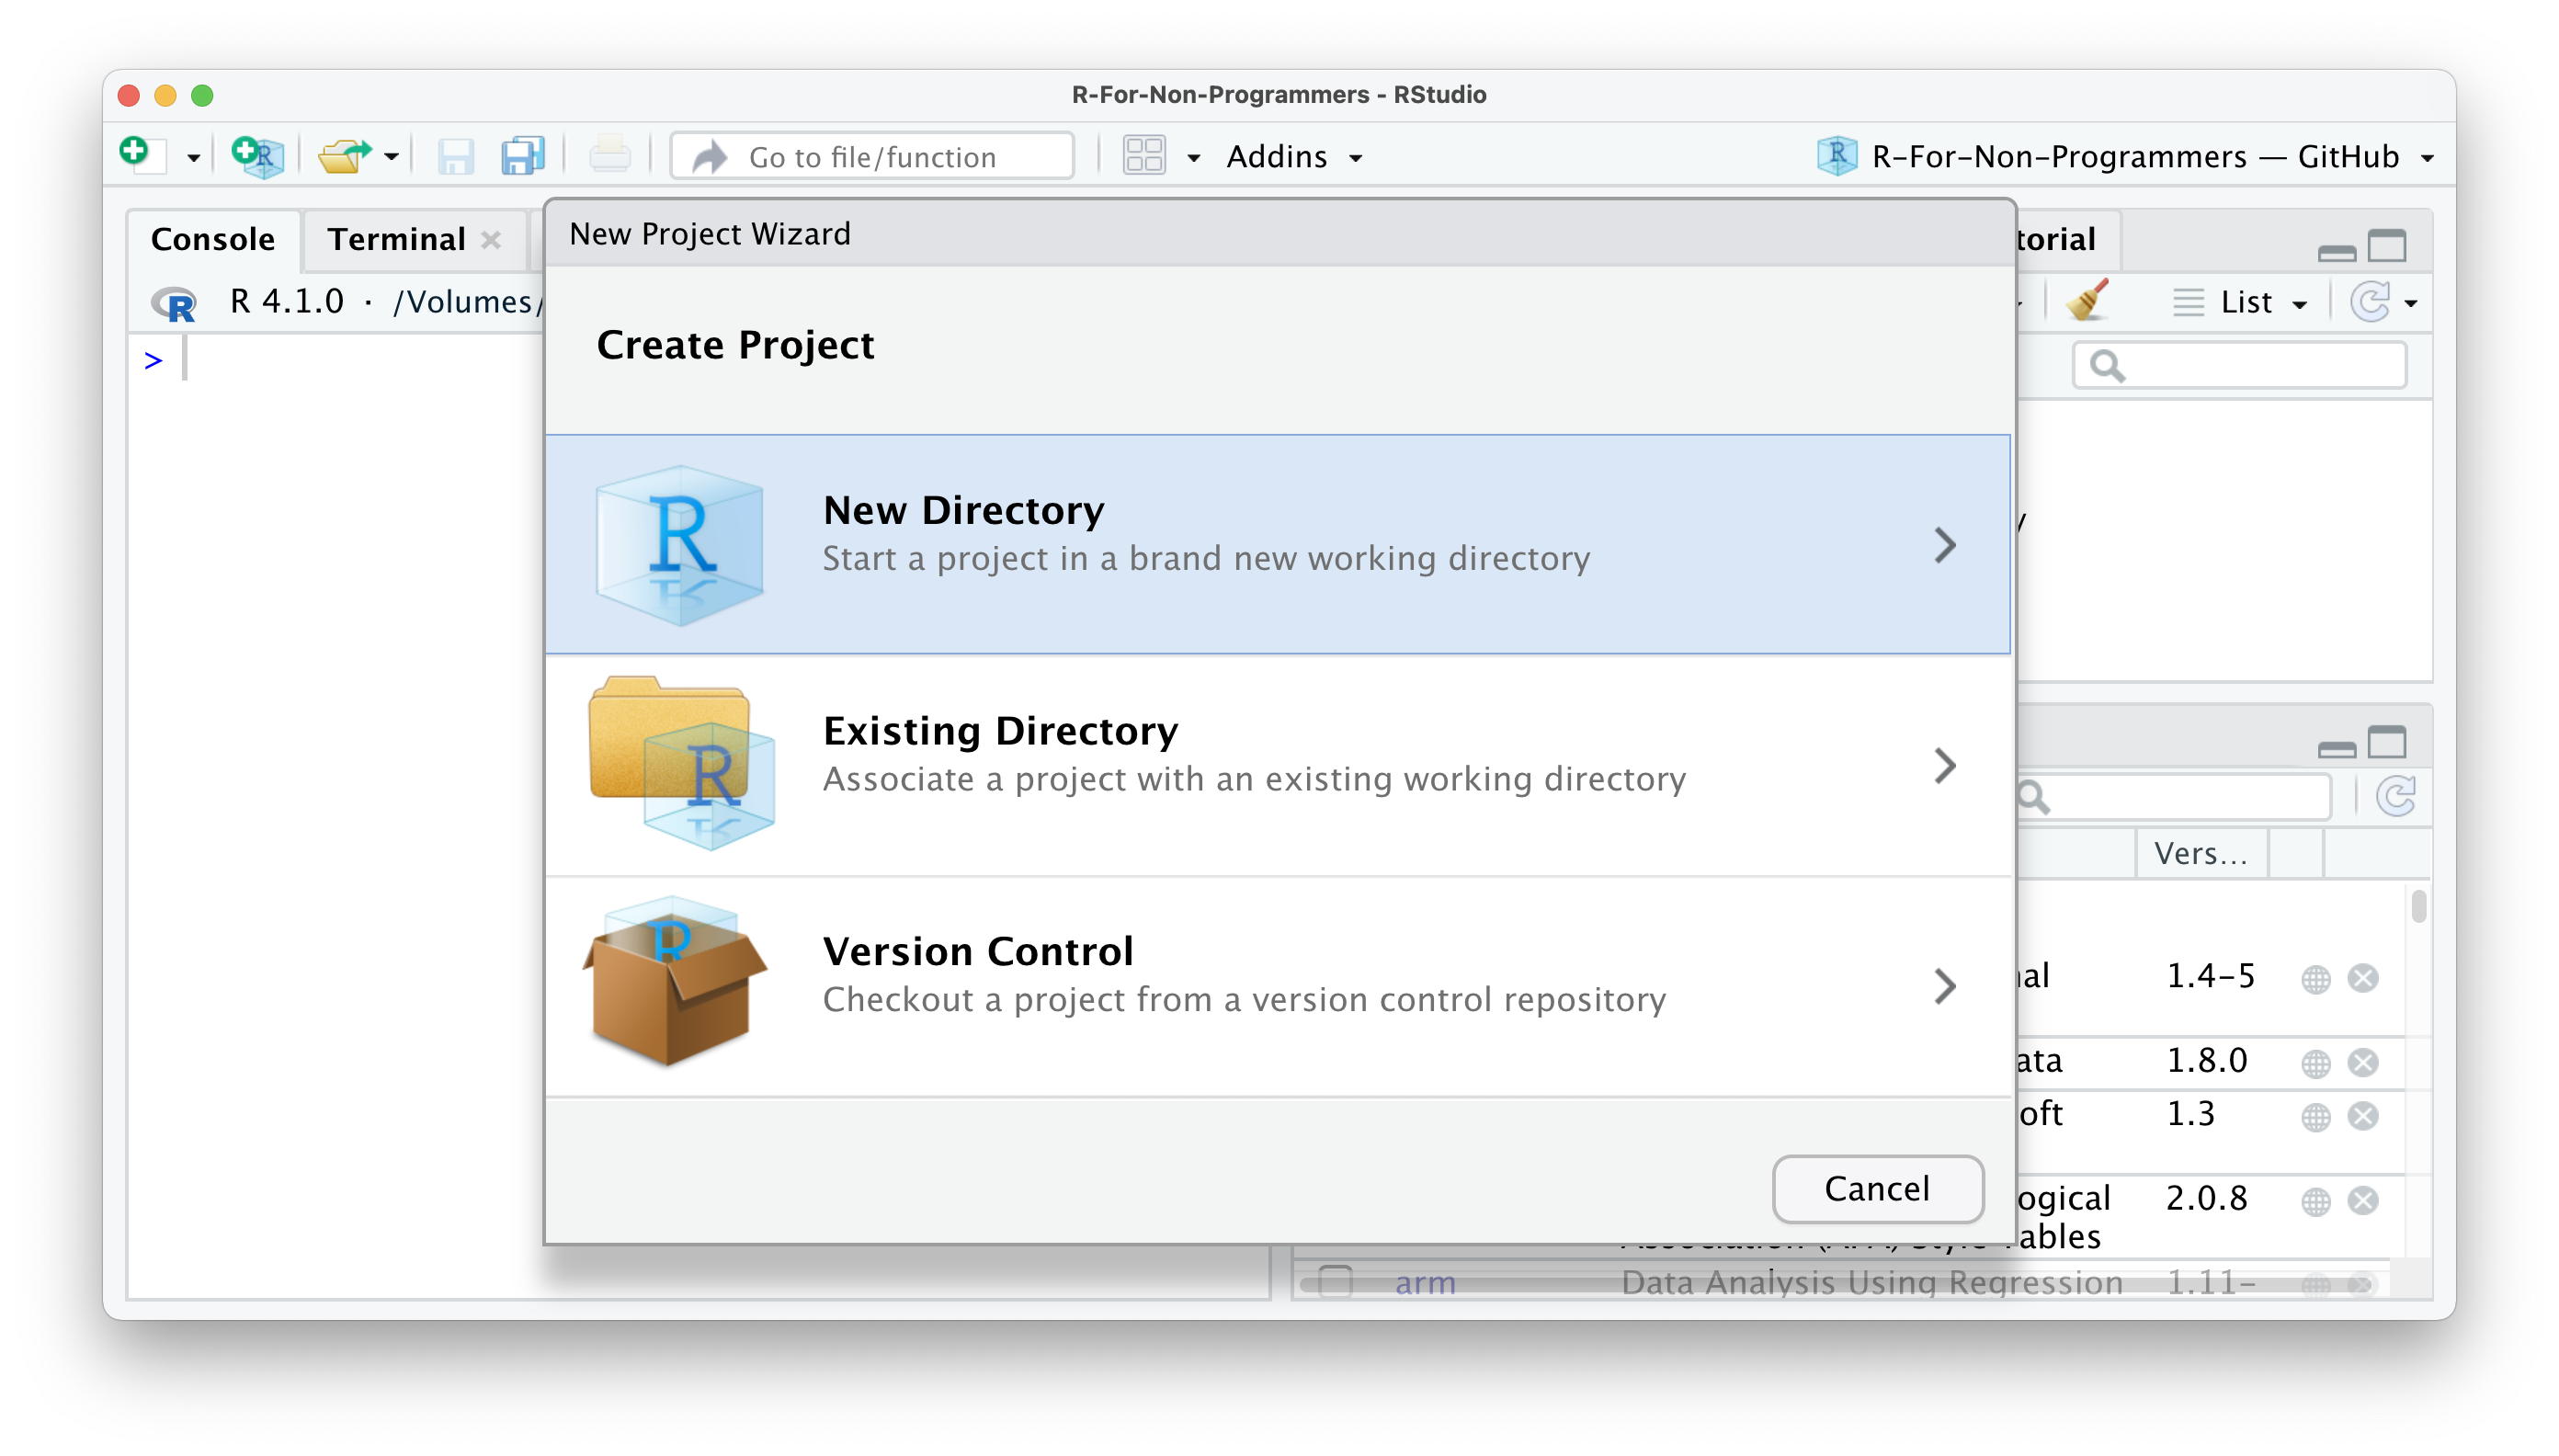
\includegraphics{images/chapter_06_img/00_r_project/01_r_project_new_directory.png}

\begin{enumerate}
\def\labelenumi{\arabic{enumi}.}
\setcounter{enumi}{2}
\tightlist
\item
  Next, select \texttt{New\ Project}.
\end{enumerate}

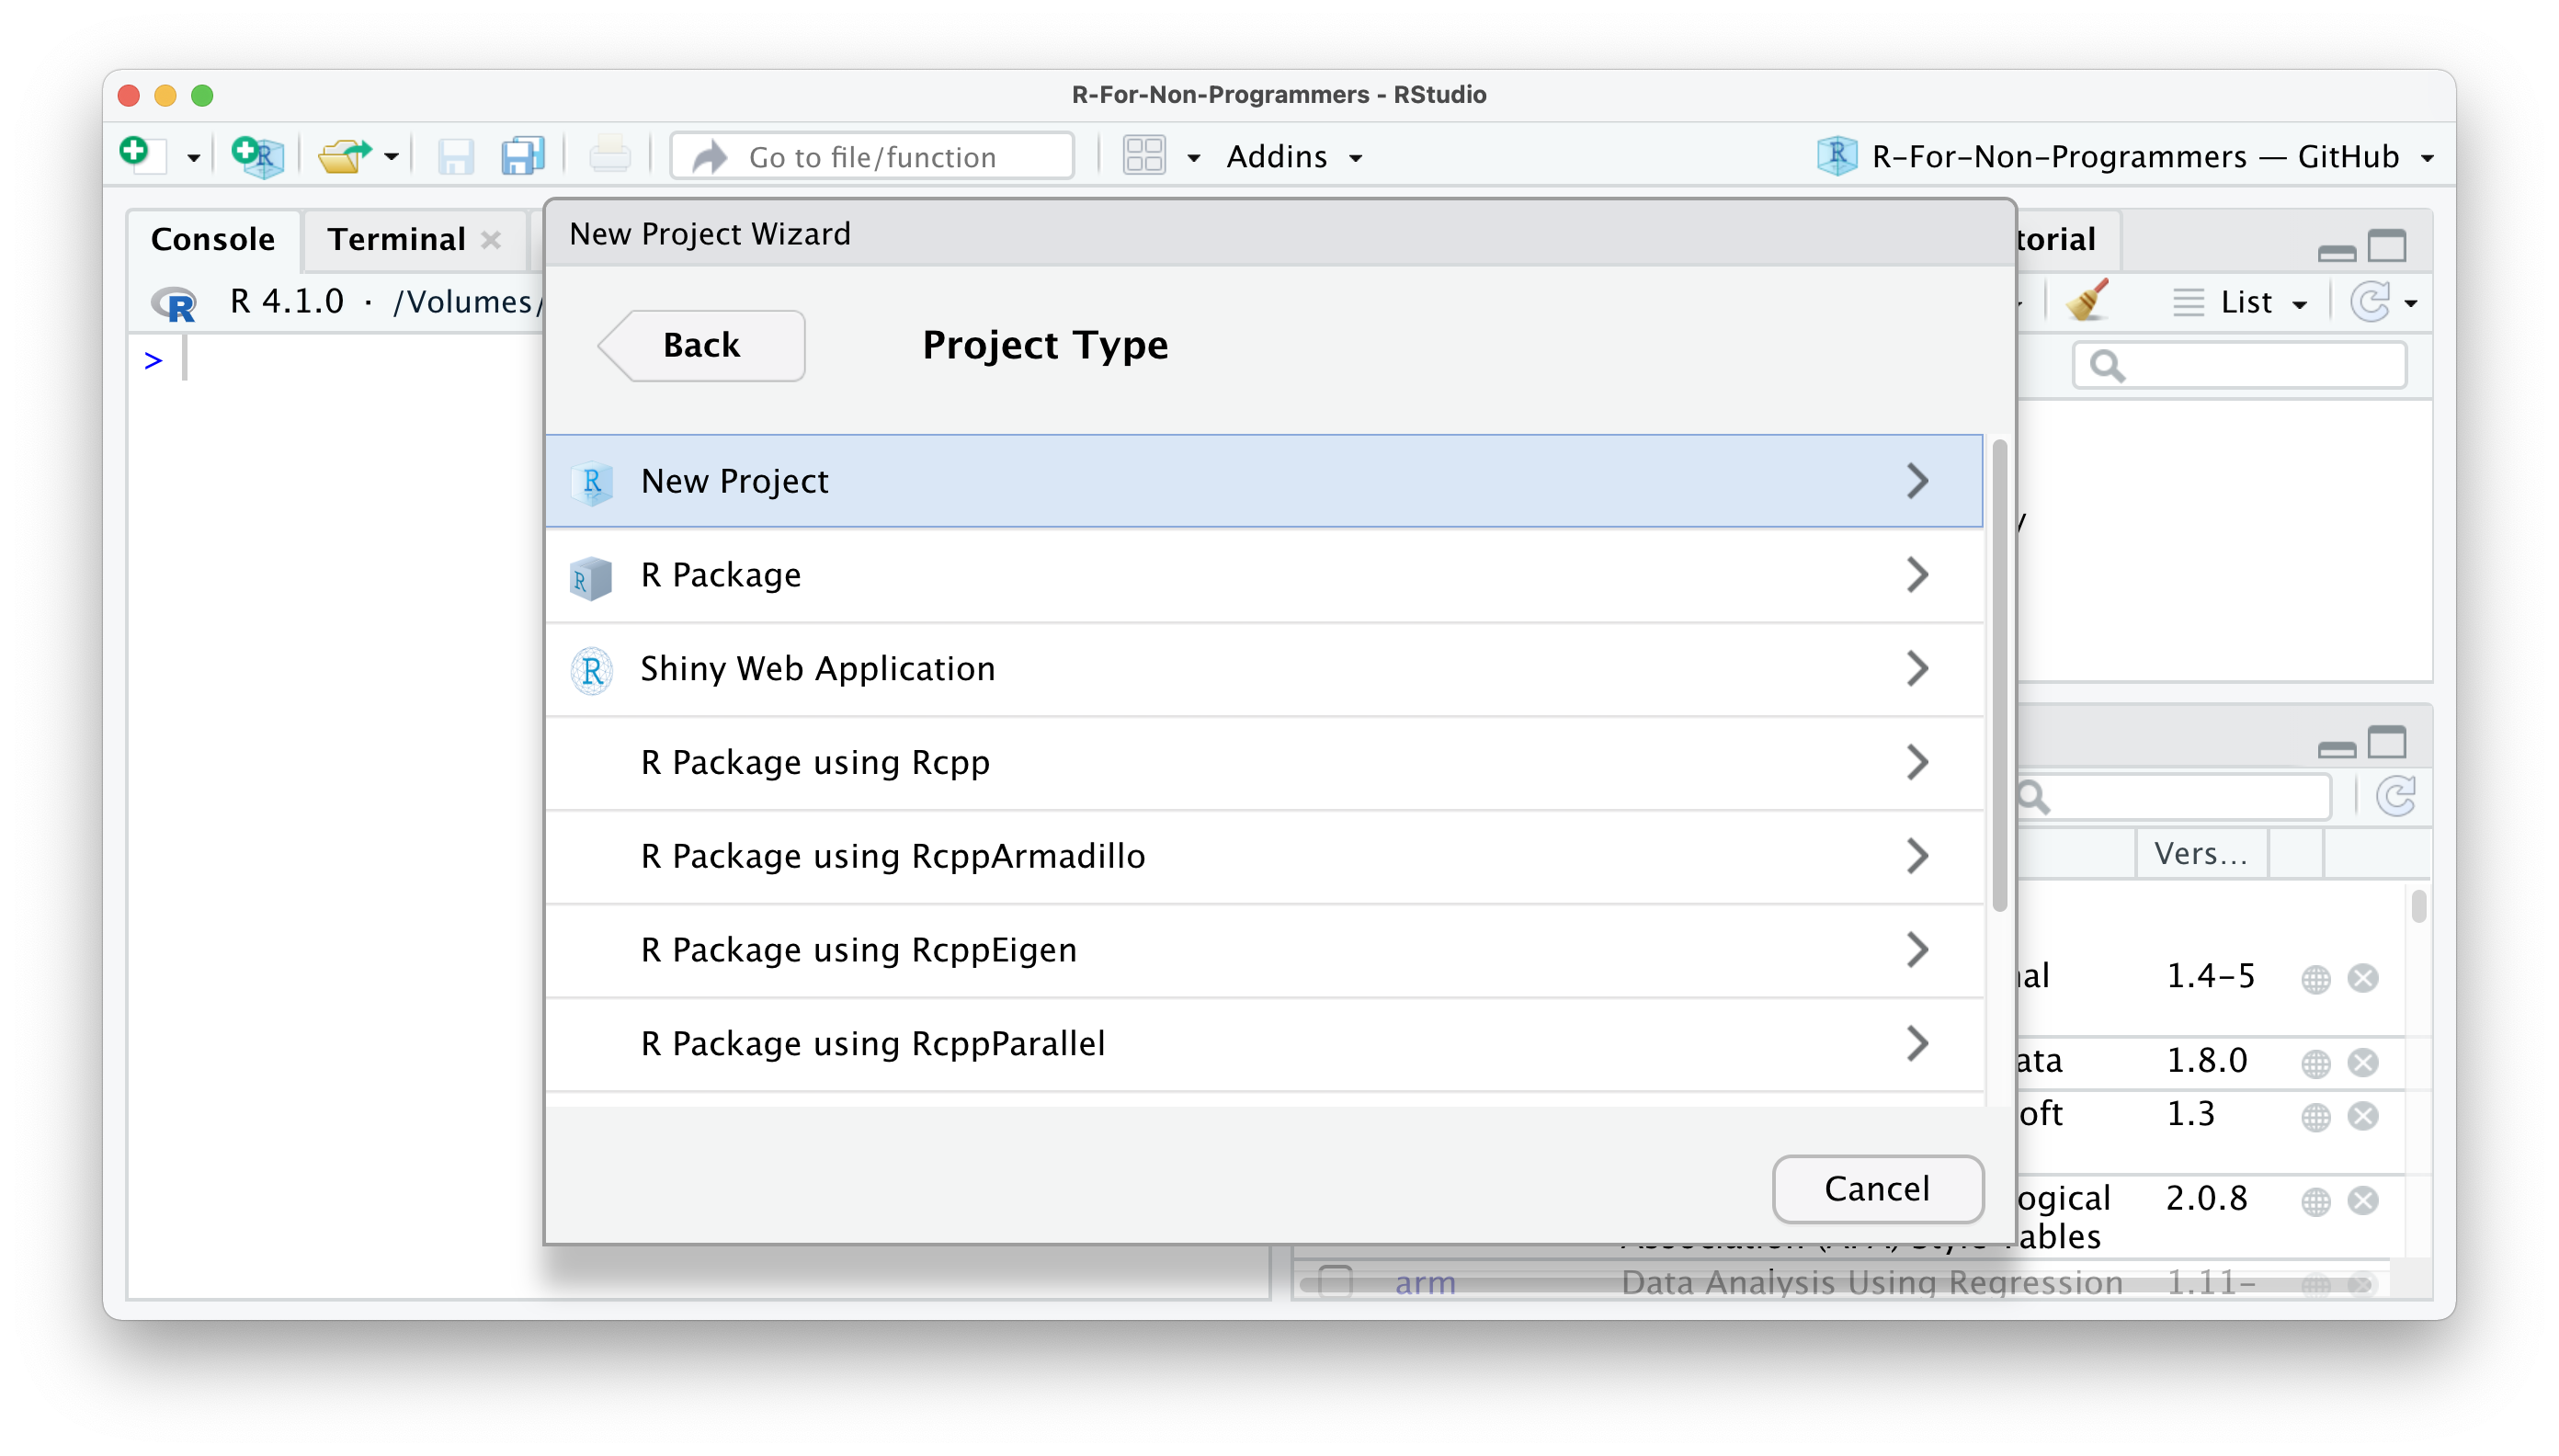
\includegraphics{images/chapter_06_img/00_r_project/02_r_project_new_project.png}

\begin{enumerate}
\def\labelenumi{\arabic{enumi}.}
\setcounter{enumi}{3}
\tightlist
\item
  Pick a meaningful name for your project folder, i.e.~the
  \texttt{Directory\ Name}. Ensure this project folder is created in the
  right place. You can change the \texttt{subdirectory} by clicking on
  \texttt{Browse…}. Ideally the subdirectory is a place where you
  usually store your research projects.
\end{enumerate}

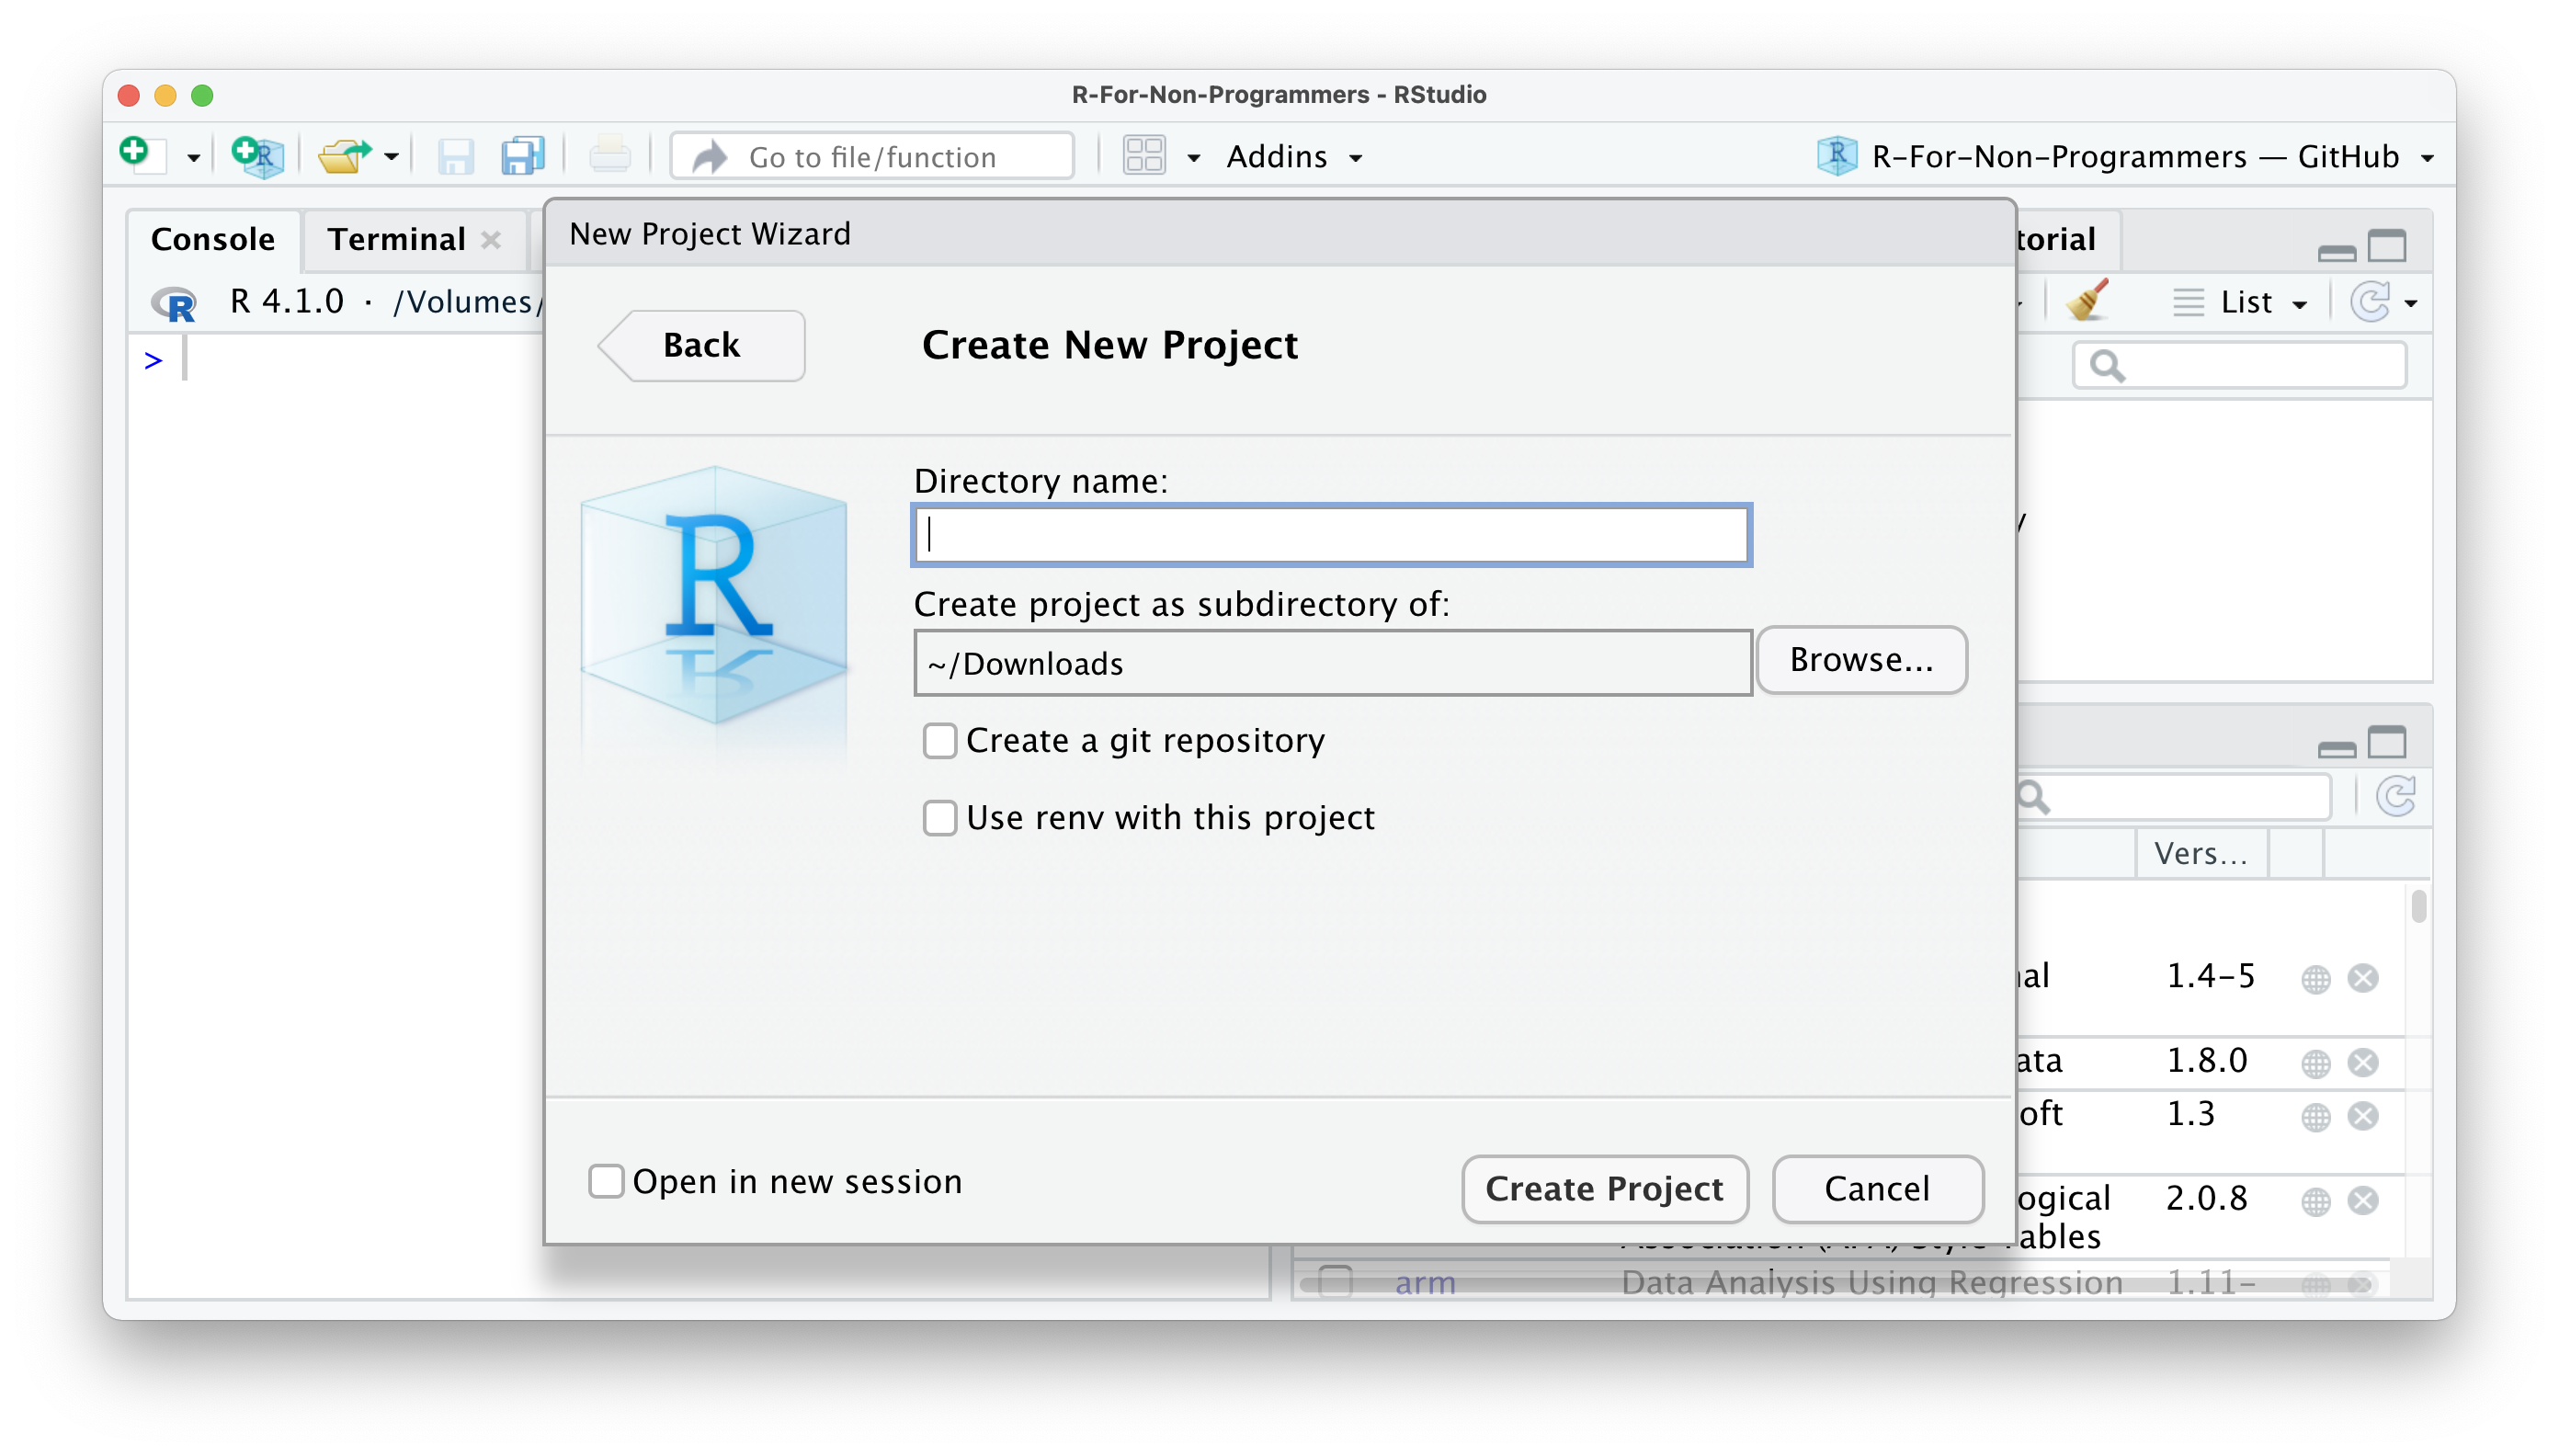
\includegraphics{images/chapter_06_img/00_r_project/03_r_project_specs.png}

\begin{enumerate}
\def\labelenumi{\arabic{enumi}.}
\setcounter{enumi}{4}
\item
  You have the option to \texttt{Create\ a\ git\ repository}. This is
  only relevant if you already have a GitHub account and wish to use
  version control. For now, you can happily ignore it if you do not use
  GitHub.
\item
  Lastly, tick \texttt{Open\ in\ new\ session}. This will open your
  \emph{R} Project in a new RStudio window.
\end{enumerate}

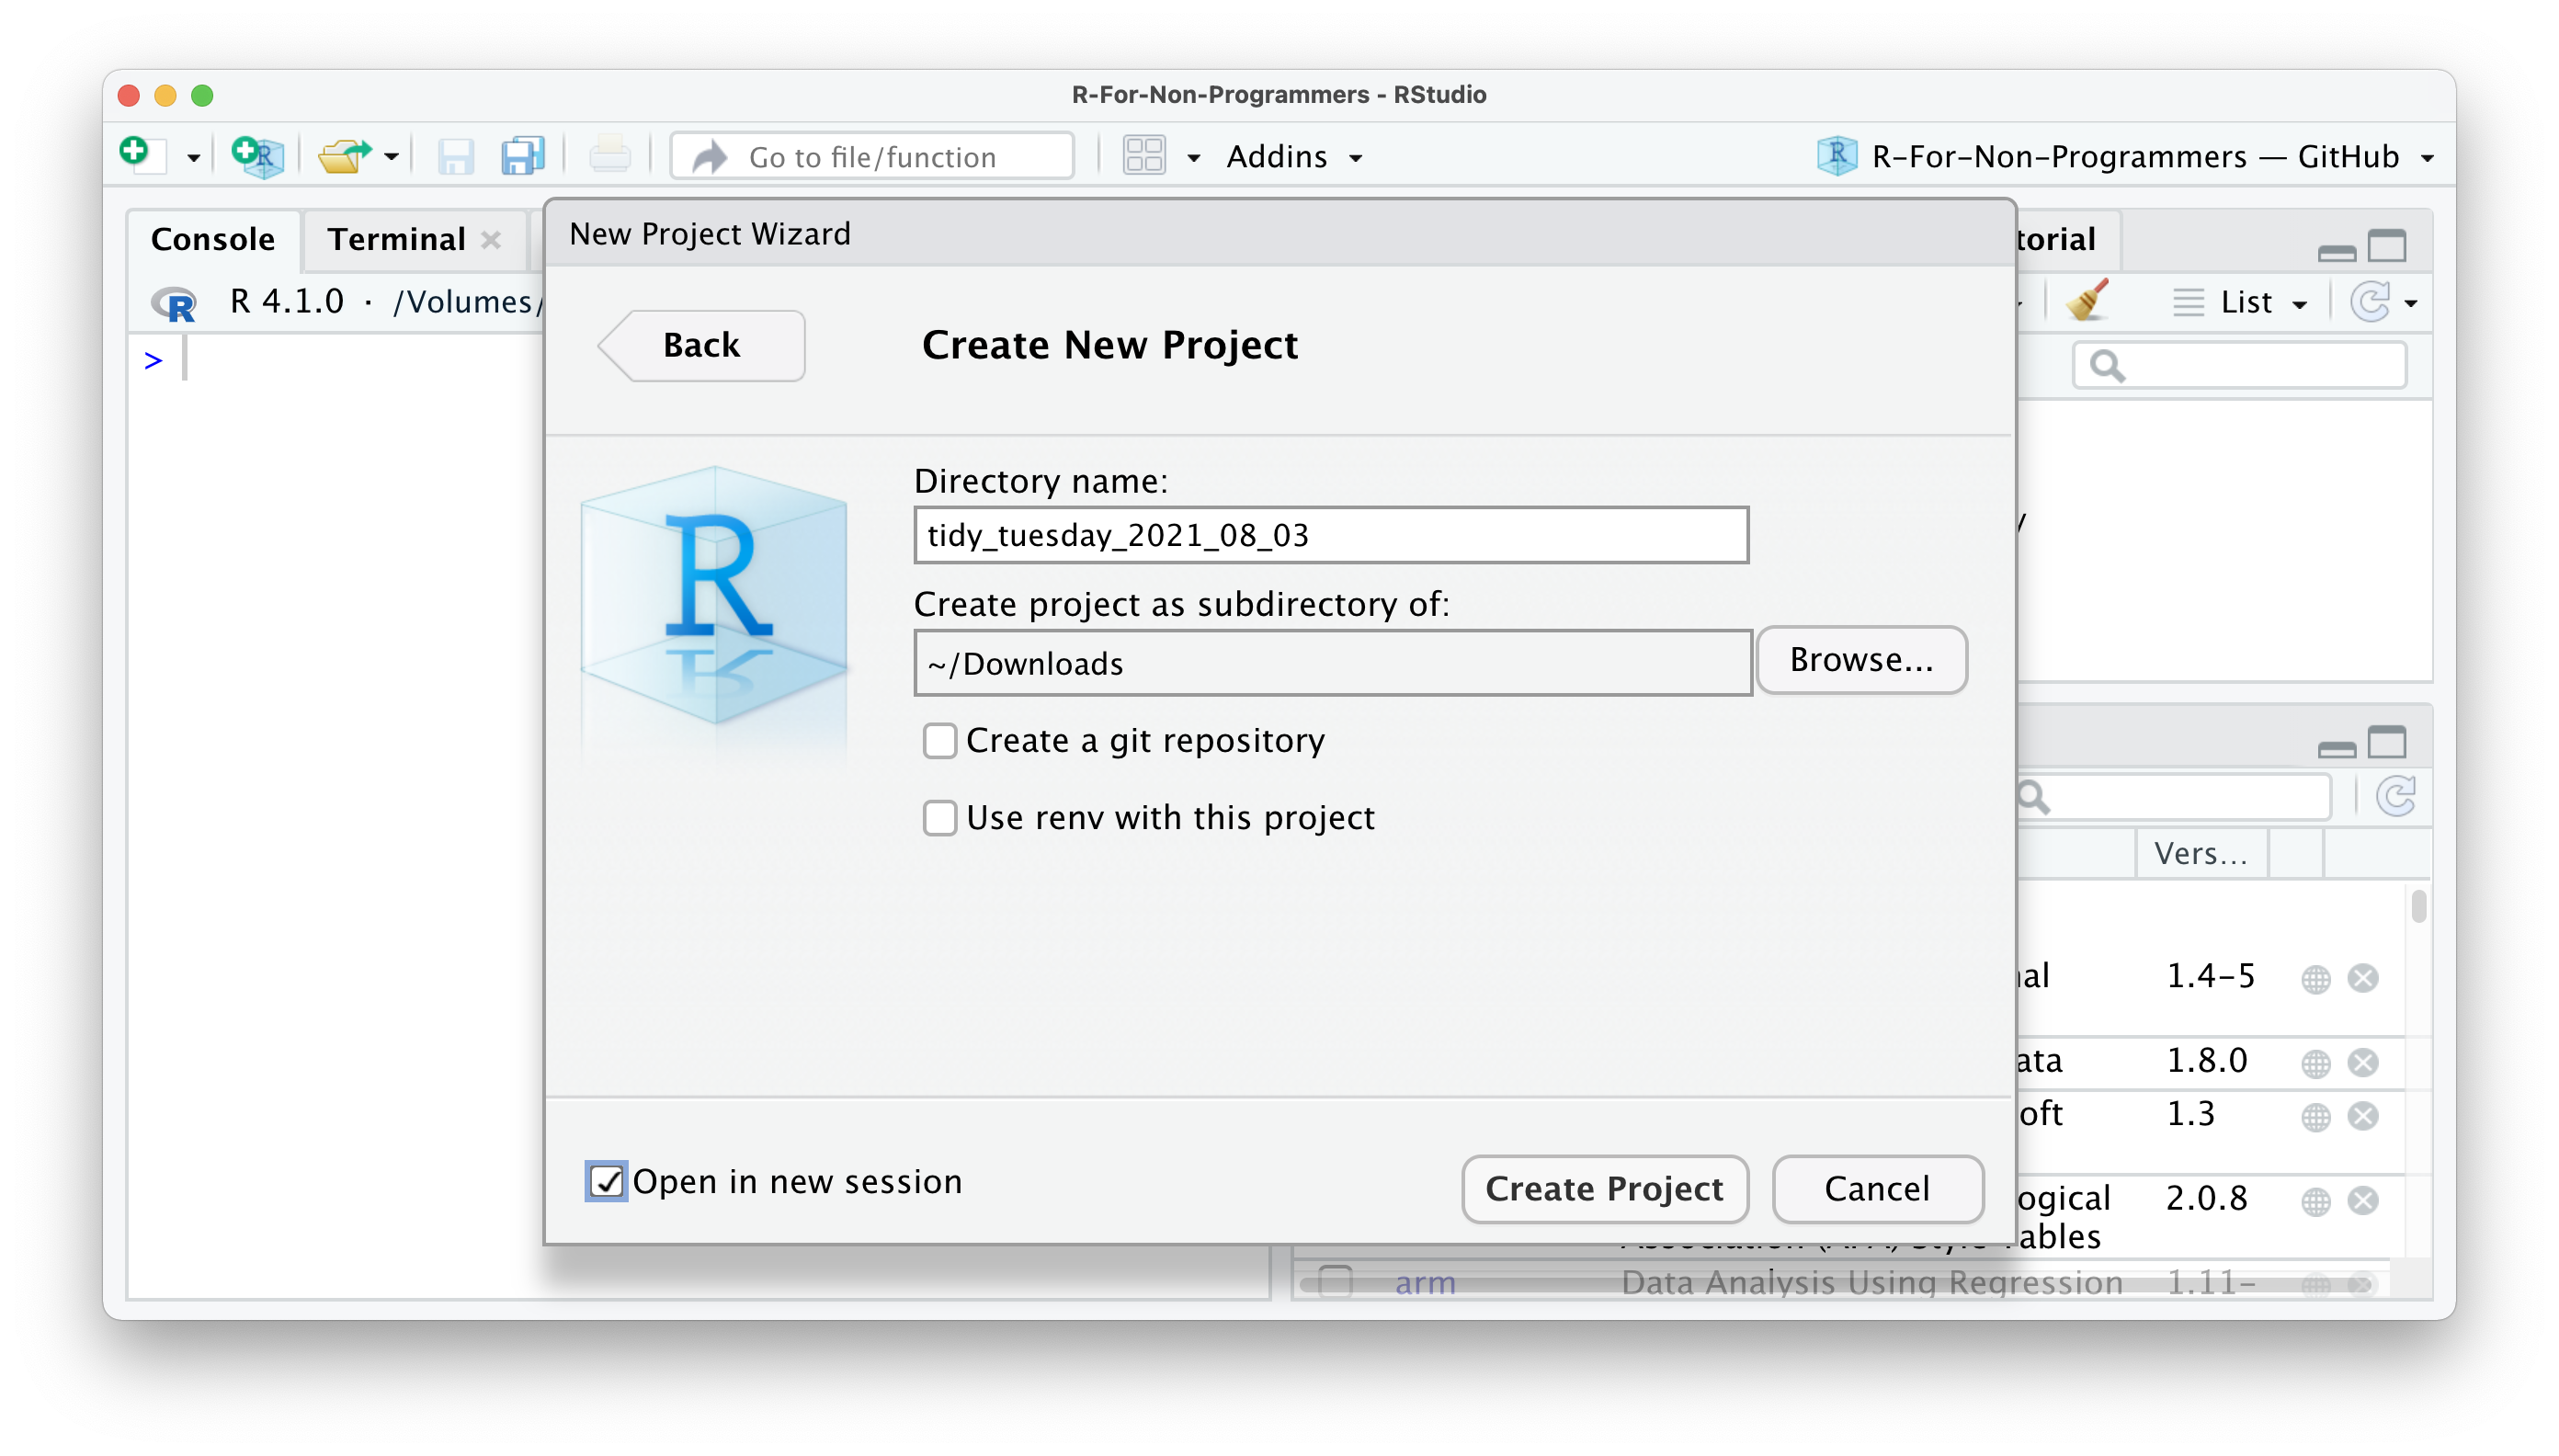
\includegraphics{images/chapter_06_img/00_r_project/04_r_project_directory_name.png}

\begin{enumerate}
\def\labelenumi{\arabic{enumi}.}
\setcounter{enumi}{6}
\tightlist
\item
  Once you are happy with your choices, you can click
  \texttt{Create\ Project}. This will open a new \emph{R} Session, and
  you can start working on your project.
\end{enumerate}

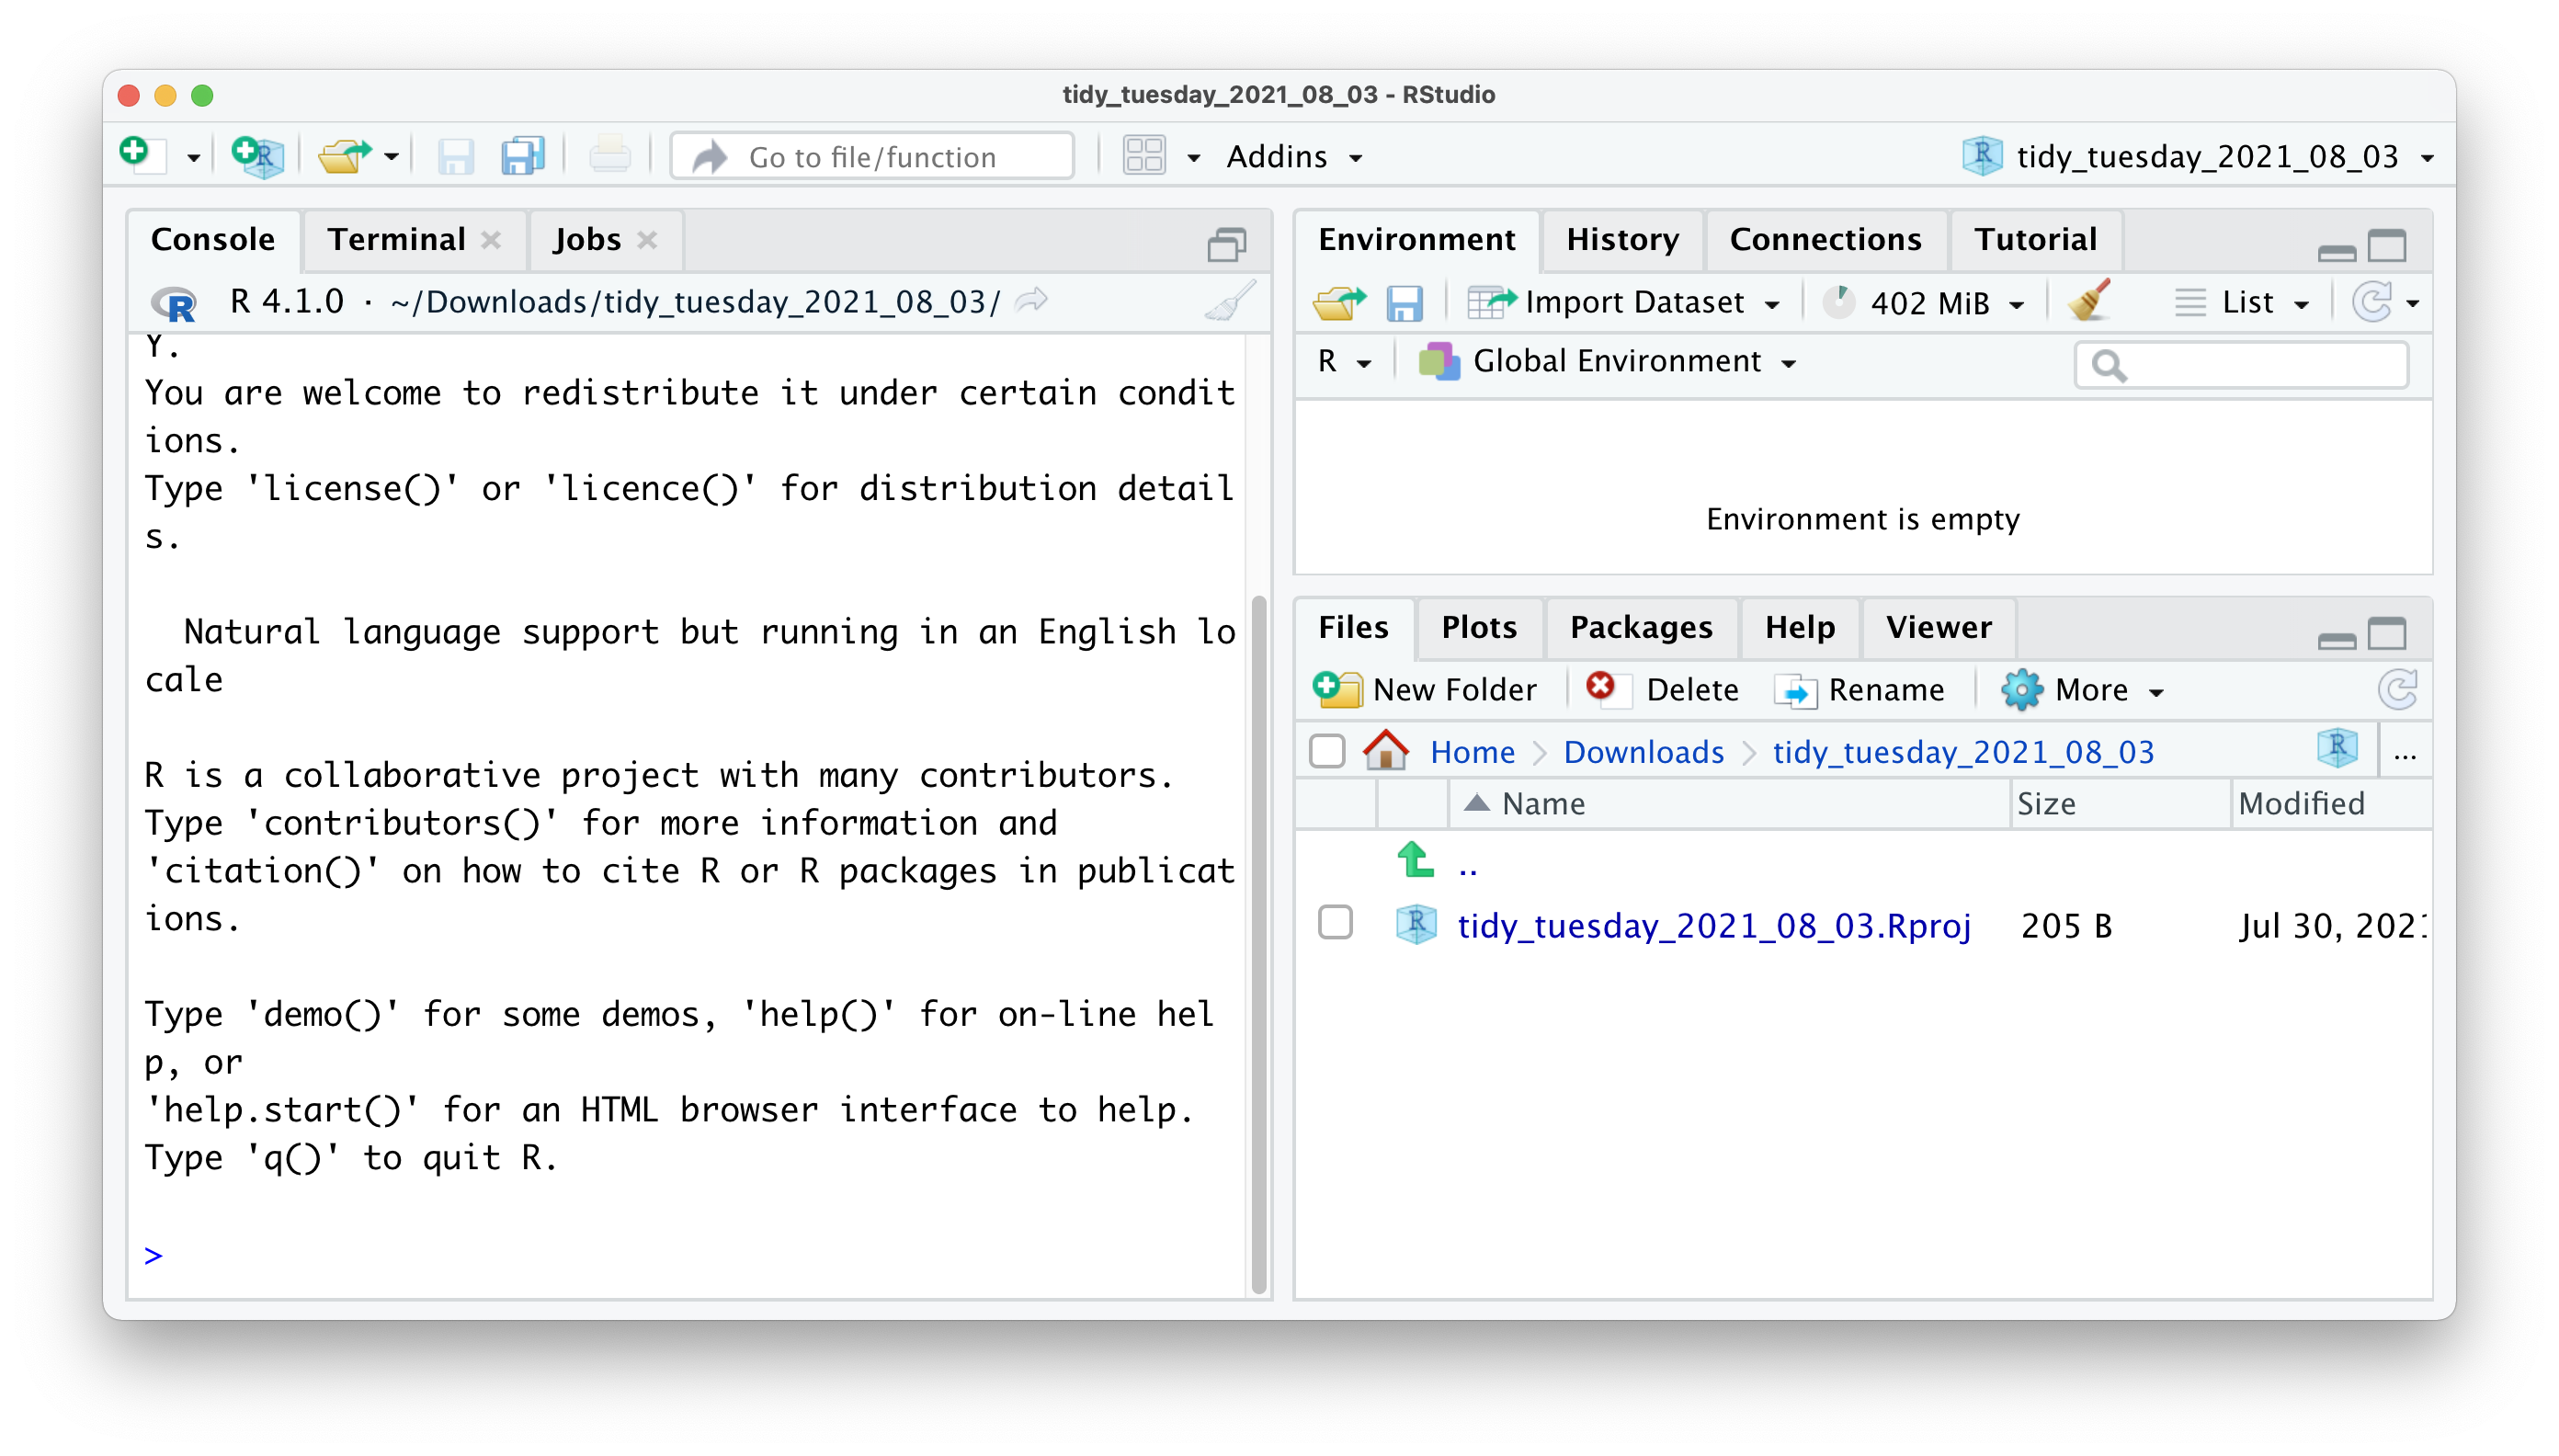
\includegraphics{images/chapter_06_img/00_r_project/05_r_project_new_session.png}

If you look carefully, you can see that your RStudio is now `branded'
with your project name. At the top of the window, you see the project
name, the files pane shows the root directory where all your files will
be, and even the console shows on top the file path of your project. You
could set all this up manually, but I would not recommend it, not the
least because it is easy and swift to work with \emph{R} Projects.

\section{Organising your projects}\label{sec-organising-your-projects}

This section is not directly related to RStudio, \emph{R} or data
analysis in general. Instead, I want to convey to you that a good folder
structure can go a long way. It is an excellent habit to start thinking
about folder structures before you start working on your project.
Placing your files into dedicated folders, rather than keeping them
loosely in one container, will speed up your work and save you from the
frustration of not finding the files you need. I have a template that I
use regularly. You can either create it from scratch in RStudio or open
your file browser and create the folders there. RStudio does not mind
which way you do it. If you want to spend less time setting this up, you
might want to use the function \texttt{create\_project\_folder()} from
the \texttt{r4np} package. It creates all the folders as shown in
Figure~\ref{fig-folder-structure}.

\begin{Shaded}
\begin{Highlighting}[]
\CommentTok{\# Install \textquotesingle{}r4np\textquotesingle{} from GitHub}
\NormalTok{devtools}\SpecialCharTok{::}\FunctionTok{install\_github}\NormalTok{(}\StringTok{"ddauber/r4np"}\NormalTok{)}

\CommentTok{\# Create the template structure}
\NormalTok{r4np}\SpecialCharTok{::}\FunctionTok{create\_project\_folder}\NormalTok{()}
\end{Highlighting}
\end{Shaded}

To create a folder, click on \texttt{New\ Folder} in the \emph{Files}
pane. I usually have at least the following folders for every project I
am involved in:

\begin{itemize}
\item
  A folder for my raw data. I store `untouched' datasets in it. With
  `untouched', I mean they have not been processed in any way and are
  usually files I downloaded from my data collection tool, e.g.~an
  online questionnaire platform.
\item
  A folder with `tidy' data. This is usually data I exported from
  \emph{R} after cleaning it, i.e.~after some basic data wrangling and
  cleaning (see Chapter~\ref{sec-data-wrangling}).
\item
  A folder for my \emph{R} scripts
\item
  A folder for my plots
\item
  A folder for reports.
\end{itemize}

Thus, in RStudio, it would look something like this:

\begin{figure}

\centering{

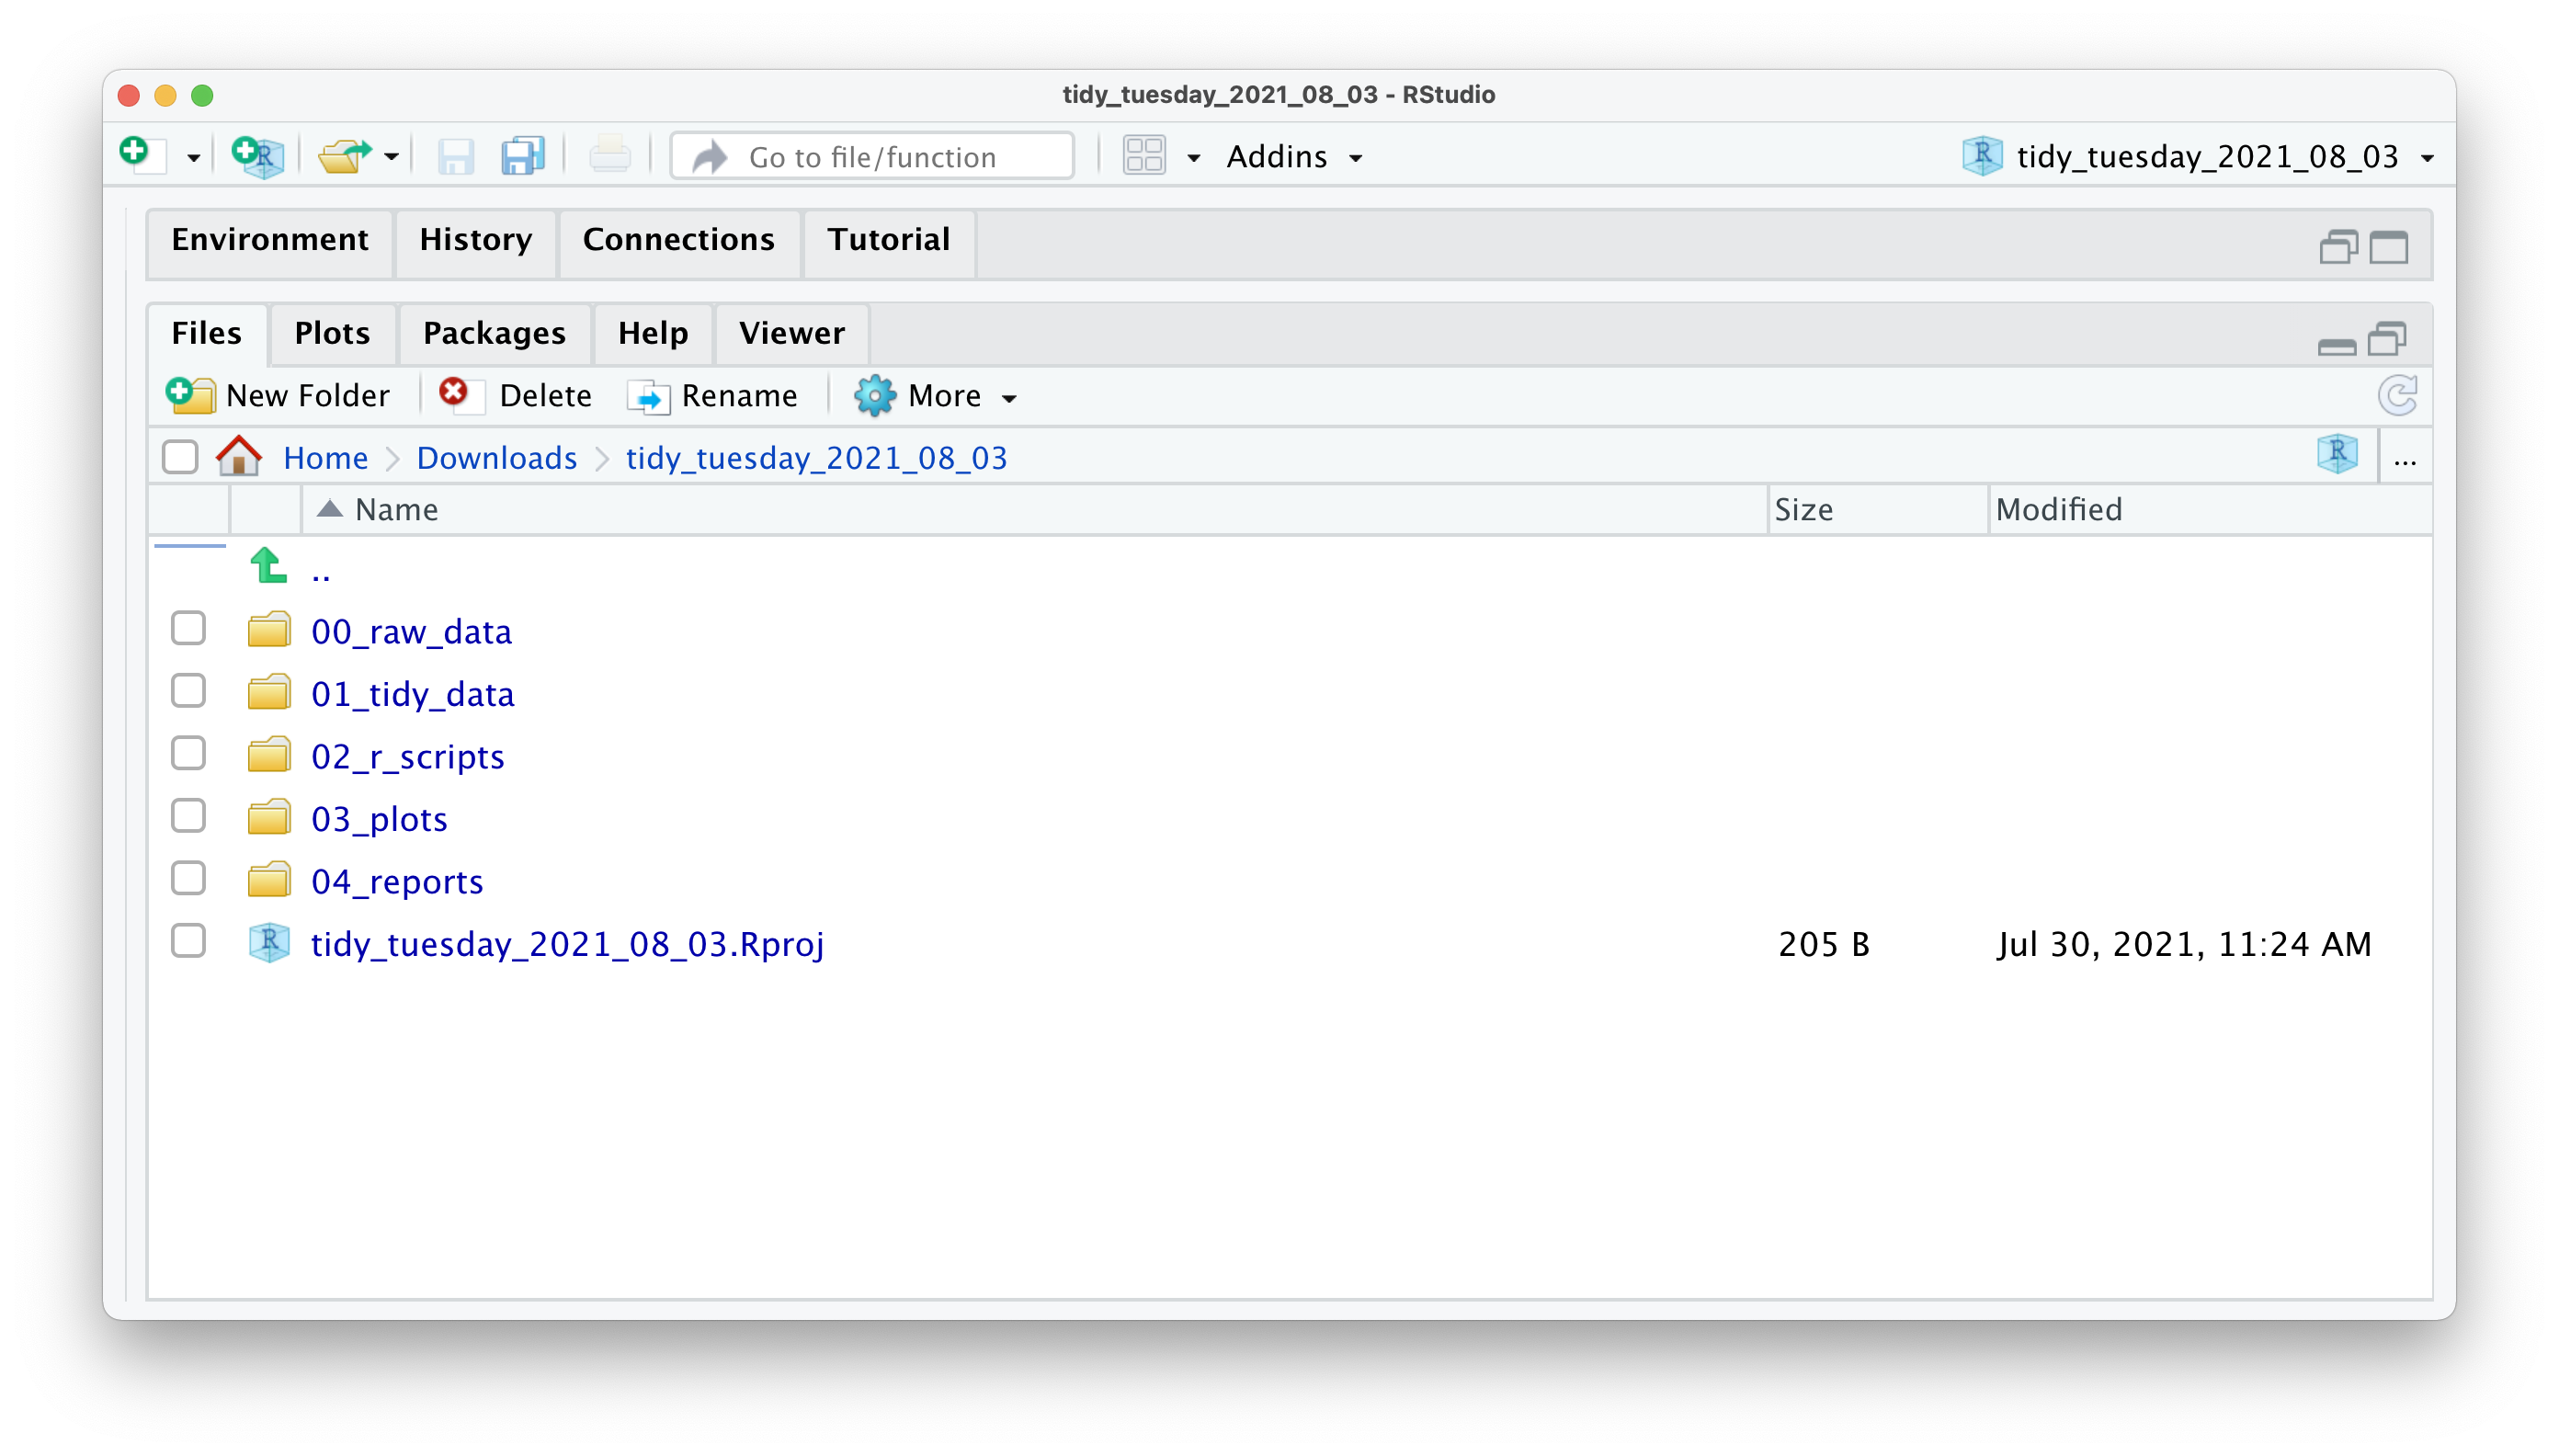
\includegraphics{images/chapter_06_img/01_organising_work/00_organising_work.png}

}

\caption{\label{fig-folder-structure}An example of a scalable folder
structure for your project}

\end{figure}%

You probably noticed that my folders have numbers in front of them. I do
this to ensure that all folders are in the order I want them to be,
which is usually not the alphabetical order my computer suggests. I use
two digits because I may have more than nine folders for a project, and
folder ten could otherwise be listed as the second folder in this list
(this depends on your operating system). With this filing strategy in
place, it will be easy to find whatever I need. Even others can easily
understand what I stored where. It is simply `tidy', similar to how we
want our data to be.

\section{\texorpdfstring{Creating an \emph{R}
Script}{Creating an R Script}}\label{sec-creating-an-r-script}

Code quickly becomes long and complex. Thus, it is not very convenient
to write it in the console. So, instead, we can write code into an
\emph{R} Script. An \emph{R} Script is a document that RStudio
recognises as \emph{R} programming code. Files that are not \emph{R}
Scripts, like \texttt{.txt}, \texttt{.rtf} or \texttt{.md}, can also be
opened in RStudio, but any code written in it will not be automatically
recognised.

When opening an \emph{R} script or creating a new one, it will display
in the \emph{Source} window (see Section~\ref{sec-the-source-window}
Some refer to this window as the `script editor'. An \emph{R} script
starts as an empty file. Good coding etiquette (see
Section~\ref{sec-coding-etiquette}) demands that we use the first line
to indicate what this file does by using a comment \texttt{\#}. Here is
an example for a \href{https://www.tidytuesday.com}{`TidyTuesday'}
\emph{R} Project.

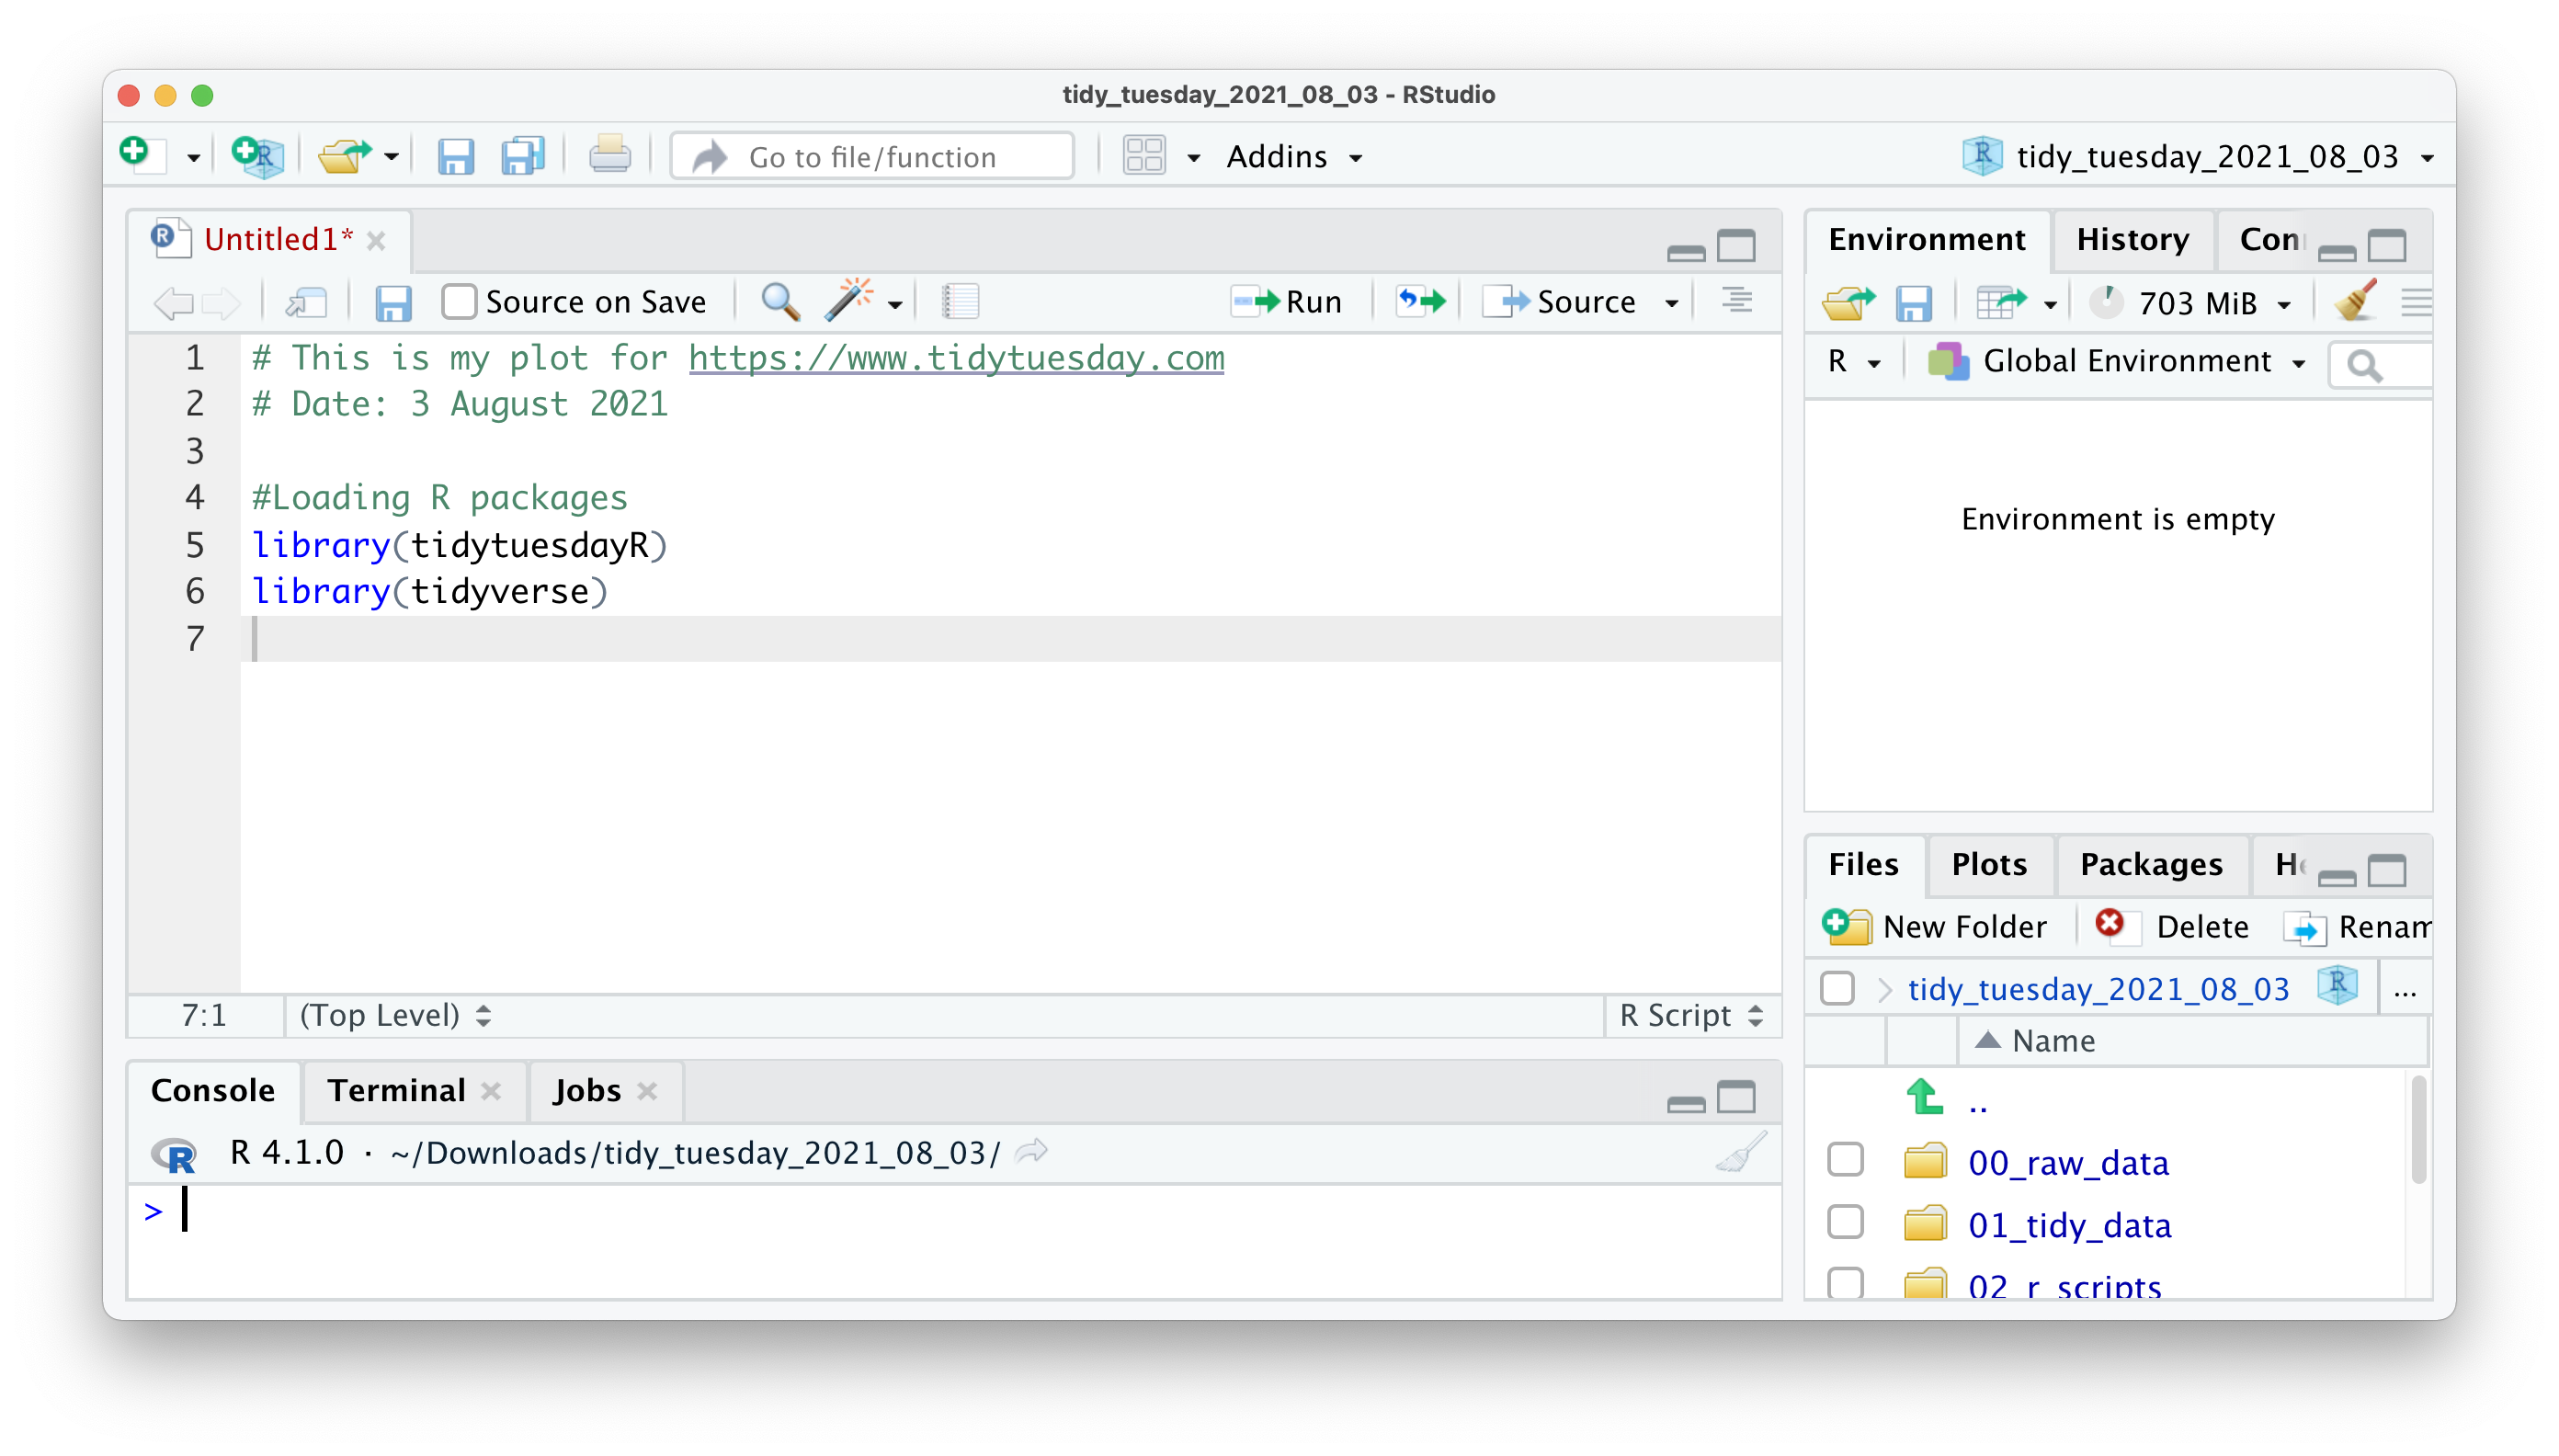
\includegraphics{images/chapter_06_img/02_r_script/00_r_script.png}

All examples in this book can easily be copied and pasted into your own
\emph{R} script. However, for some code you will have to install the
\emph{R} package \texttt{r4np} (see \hyperref[install_r4np]{above}).
Let's try it with the following code. The plot this code creates reveals
which car manufacturer produces the most efficient cars. Copy and paste
this code into your \emph{R} script.

\begin{Shaded}
\begin{Highlighting}[]
\FunctionTok{library}\NormalTok{(tidyverse)}

\NormalTok{mpg }\SpecialCharTok{|\textgreater{}} \FunctionTok{ggplot}\NormalTok{(}\FunctionTok{aes}\NormalTok{(}\AttributeTok{x =} \FunctionTok{reorder}\NormalTok{(manufacturer, }\FunctionTok{desc}\NormalTok{(hwy), }\AttributeTok{FUN =}\NormalTok{ median),}
                   \AttributeTok{y =}\NormalTok{ hwy,}
                   \AttributeTok{fill =}\NormalTok{ manufacturer)) }\SpecialCharTok{+}
  \FunctionTok{geom\_boxplot}\NormalTok{() }\SpecialCharTok{+}
  \FunctionTok{coord\_flip}\NormalTok{() }\SpecialCharTok{+}
  \FunctionTok{theme\_minimal}\NormalTok{() }\SpecialCharTok{+}
  \FunctionTok{xlab}\NormalTok{(}\StringTok{"Manufacturer"}\NormalTok{) }\SpecialCharTok{+}
  \FunctionTok{ylab}\NormalTok{(}\StringTok{"Highway miles per gallon"}\NormalTok{)}
\end{Highlighting}
\end{Shaded}

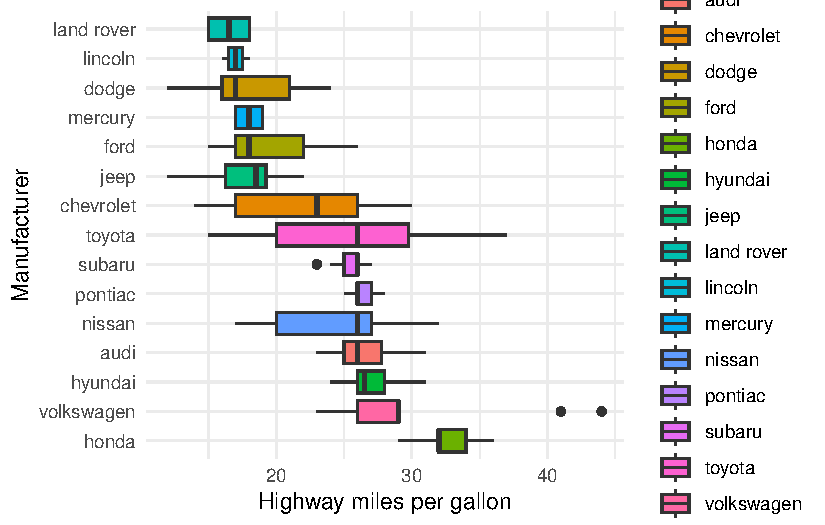
\includegraphics{06_starting_r_projects_files/figure-latex/r-script-copy-paste-examples-1.pdf}

You are probably wondering where your plot has gone. Copying the code
will not automatically run it in your \emph{R} script. However, this is
necessary to create the plot. If you tried pressing \texttt{Return}, you
would only add a new line. Instead, you need to select the code you want
to run and press \texttt{Ctrl+Return} (PC) or \texttt{Cmd+Return} (Mac).
You can also use the \texttt{Run} command at the top of your source
window, but it is much more efficient to press the keyboard shortcut.
Besides, you will remember this shortcut quickly, because we need to use
it very frequently. If all worked out, you should see the following:

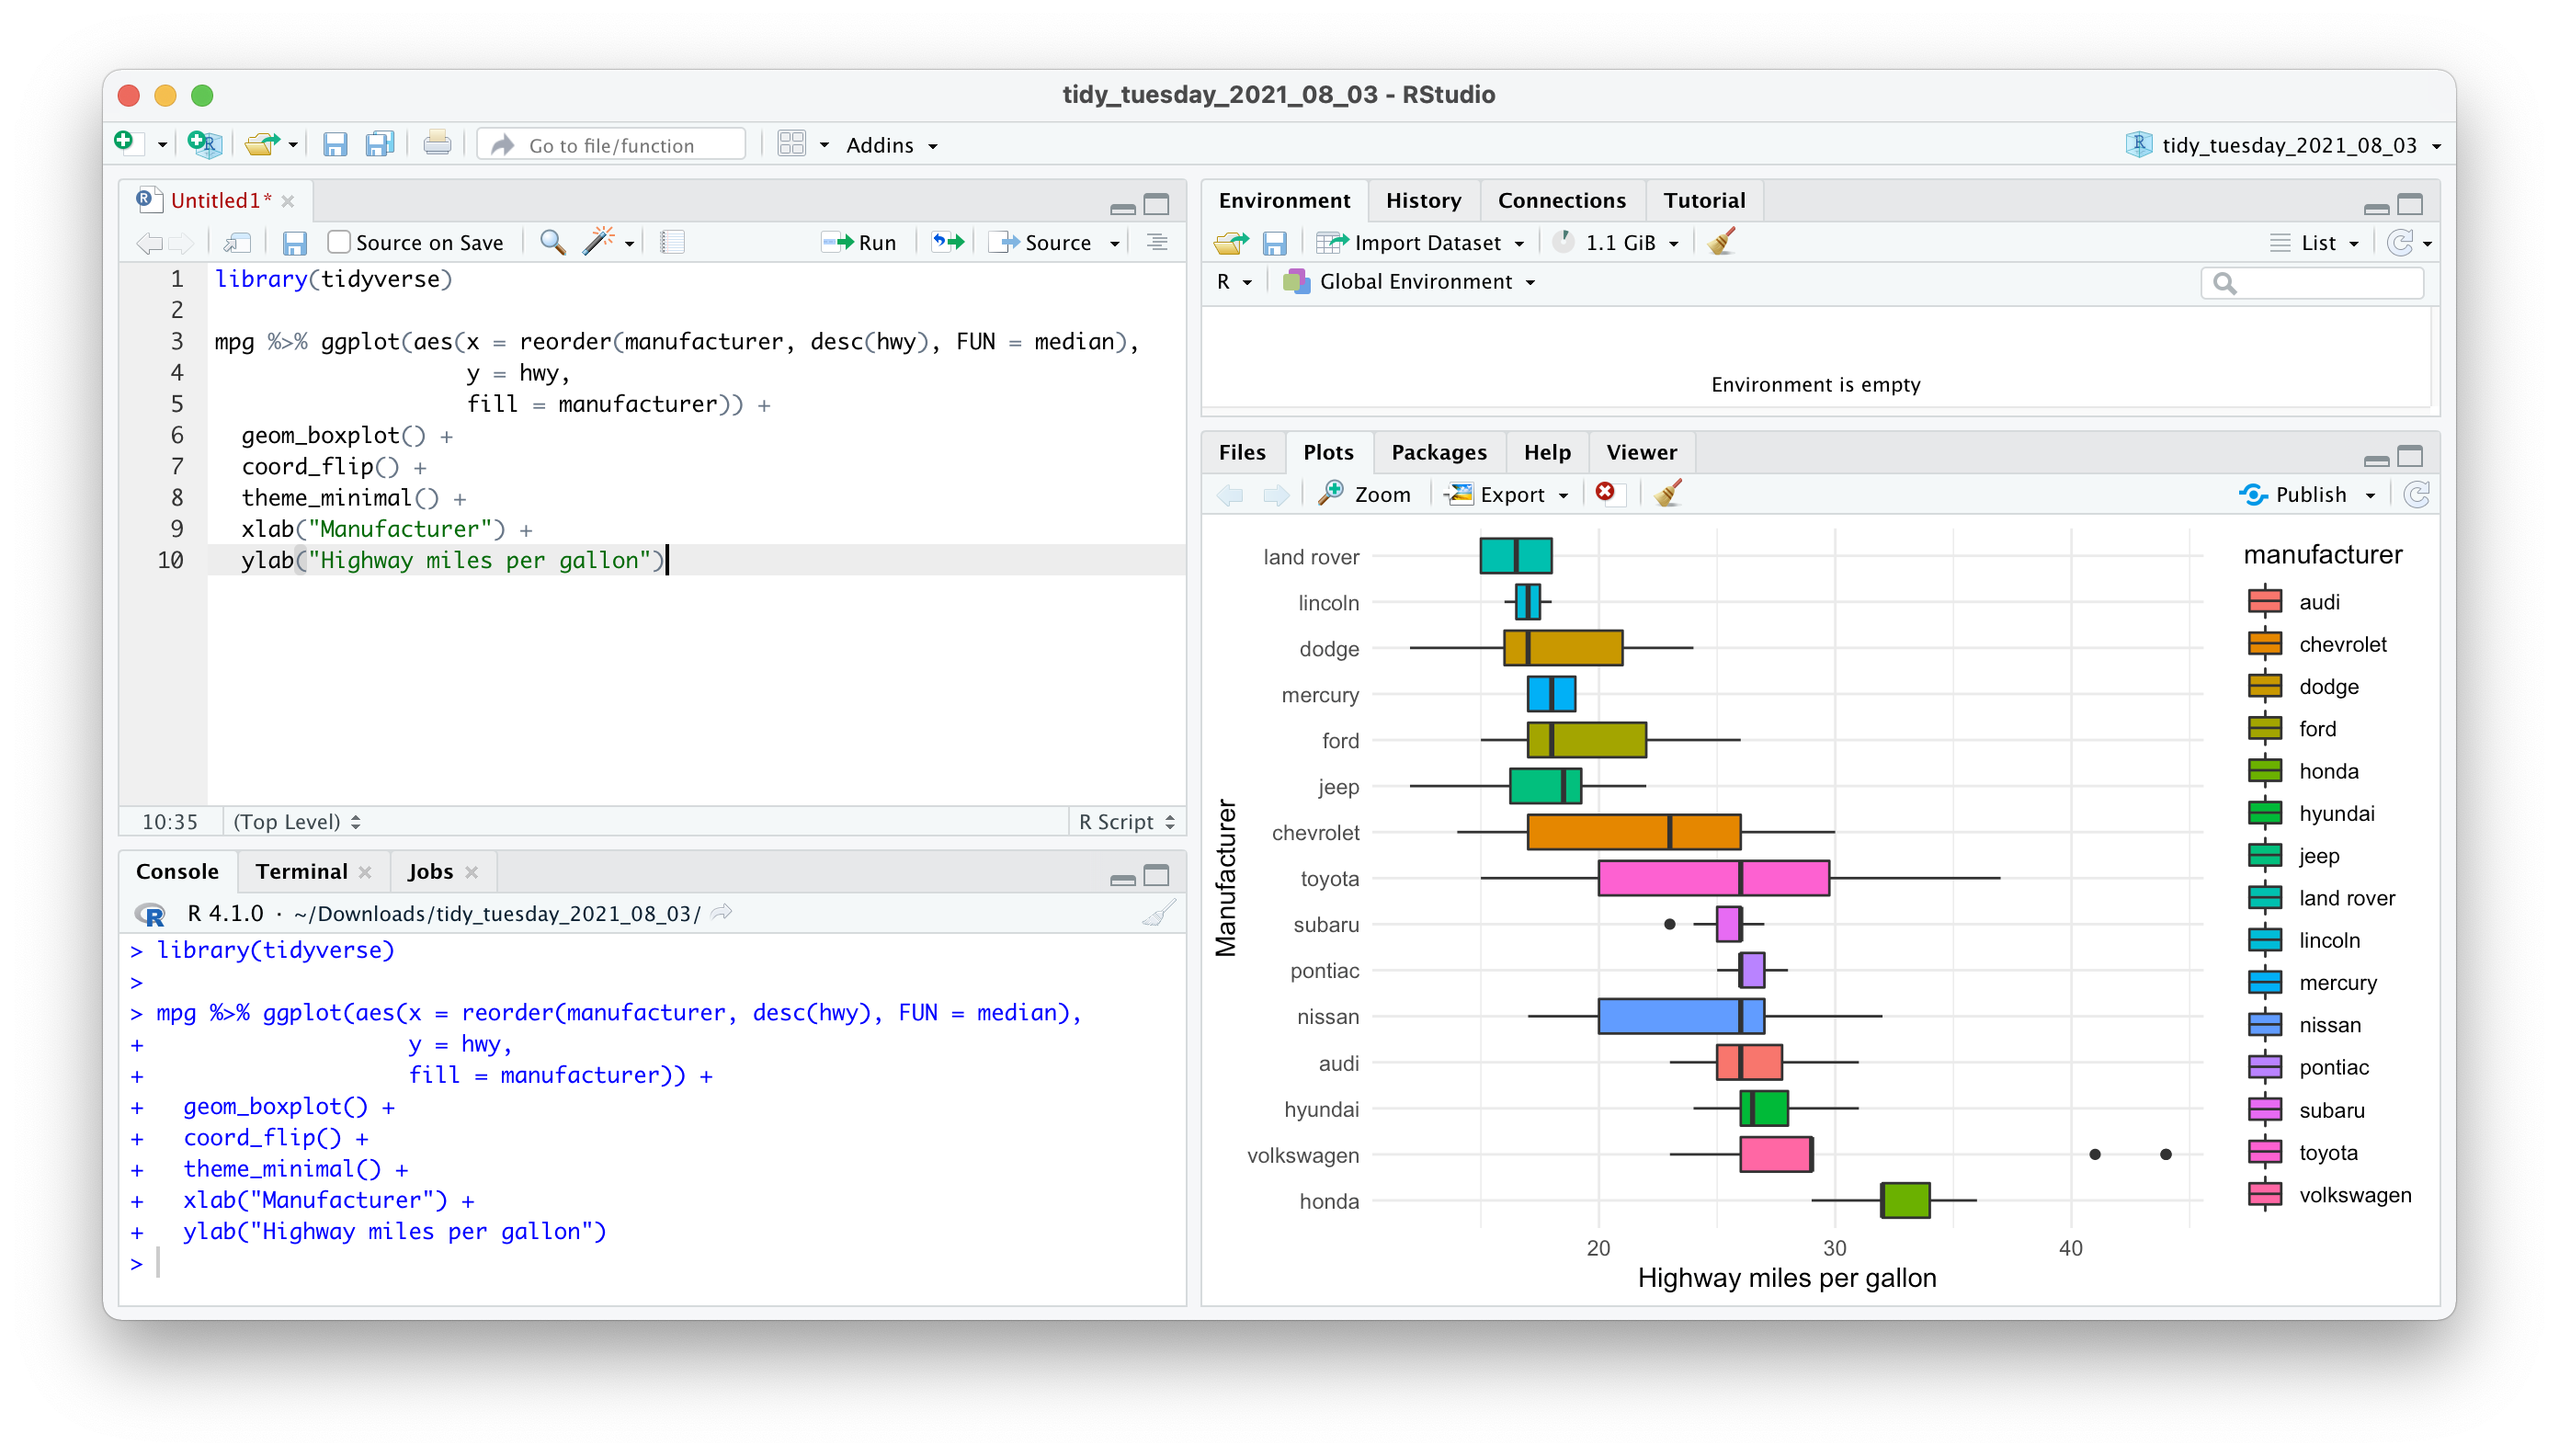
\includegraphics{images/chapter_06_img/02_r_script/01_r_script_example_plot.png}

As you can see, cars from \texttt{Honda} appear to drive furthest with
the same amount of fuel (a gallon) compared to other vehicles. Thus, if
you are looking for very economical cars, you now know where to find
them.

The \emph{R} script editor has some conveniences for writing your code
that are worth pointing out. You probably noticed that some of the code
we have pasted is blue, and some other code is in green. These colours
help to make your code more readable because they carry a specific
meaning. In the default settings, green stands for any values in
\texttt{""}, which usually stands for \texttt{character}s. Automatic
colouring of our progamming code is also called \emph{`syntax
highlighting'}.

Moreover, code in \emph{R} scripts will be automatically indented to
facilitate reading. If, for whatever reason, the indentation does not
happen, or you accidentally undo it, you can reindent a line with
\texttt{Ctrl+I} (PC) or \texttt{Cmd+I} (Mac).

Lastly, the console and the \emph{R} script editor both feature code
completion. This means that when you start typing the name of a
function, \emph{R} will provide suggestions. These are extremely helpful
and make programming a lot faster. Once you found the function you were
looking for, you press \texttt{Return} to insert it. Here is an example
of what happens when you have the package \texttt{tidyverse} loaded and
type \texttt{ggpl}. Only functions that are loaded via packages or any
object in your environment pane benefit from code completion.

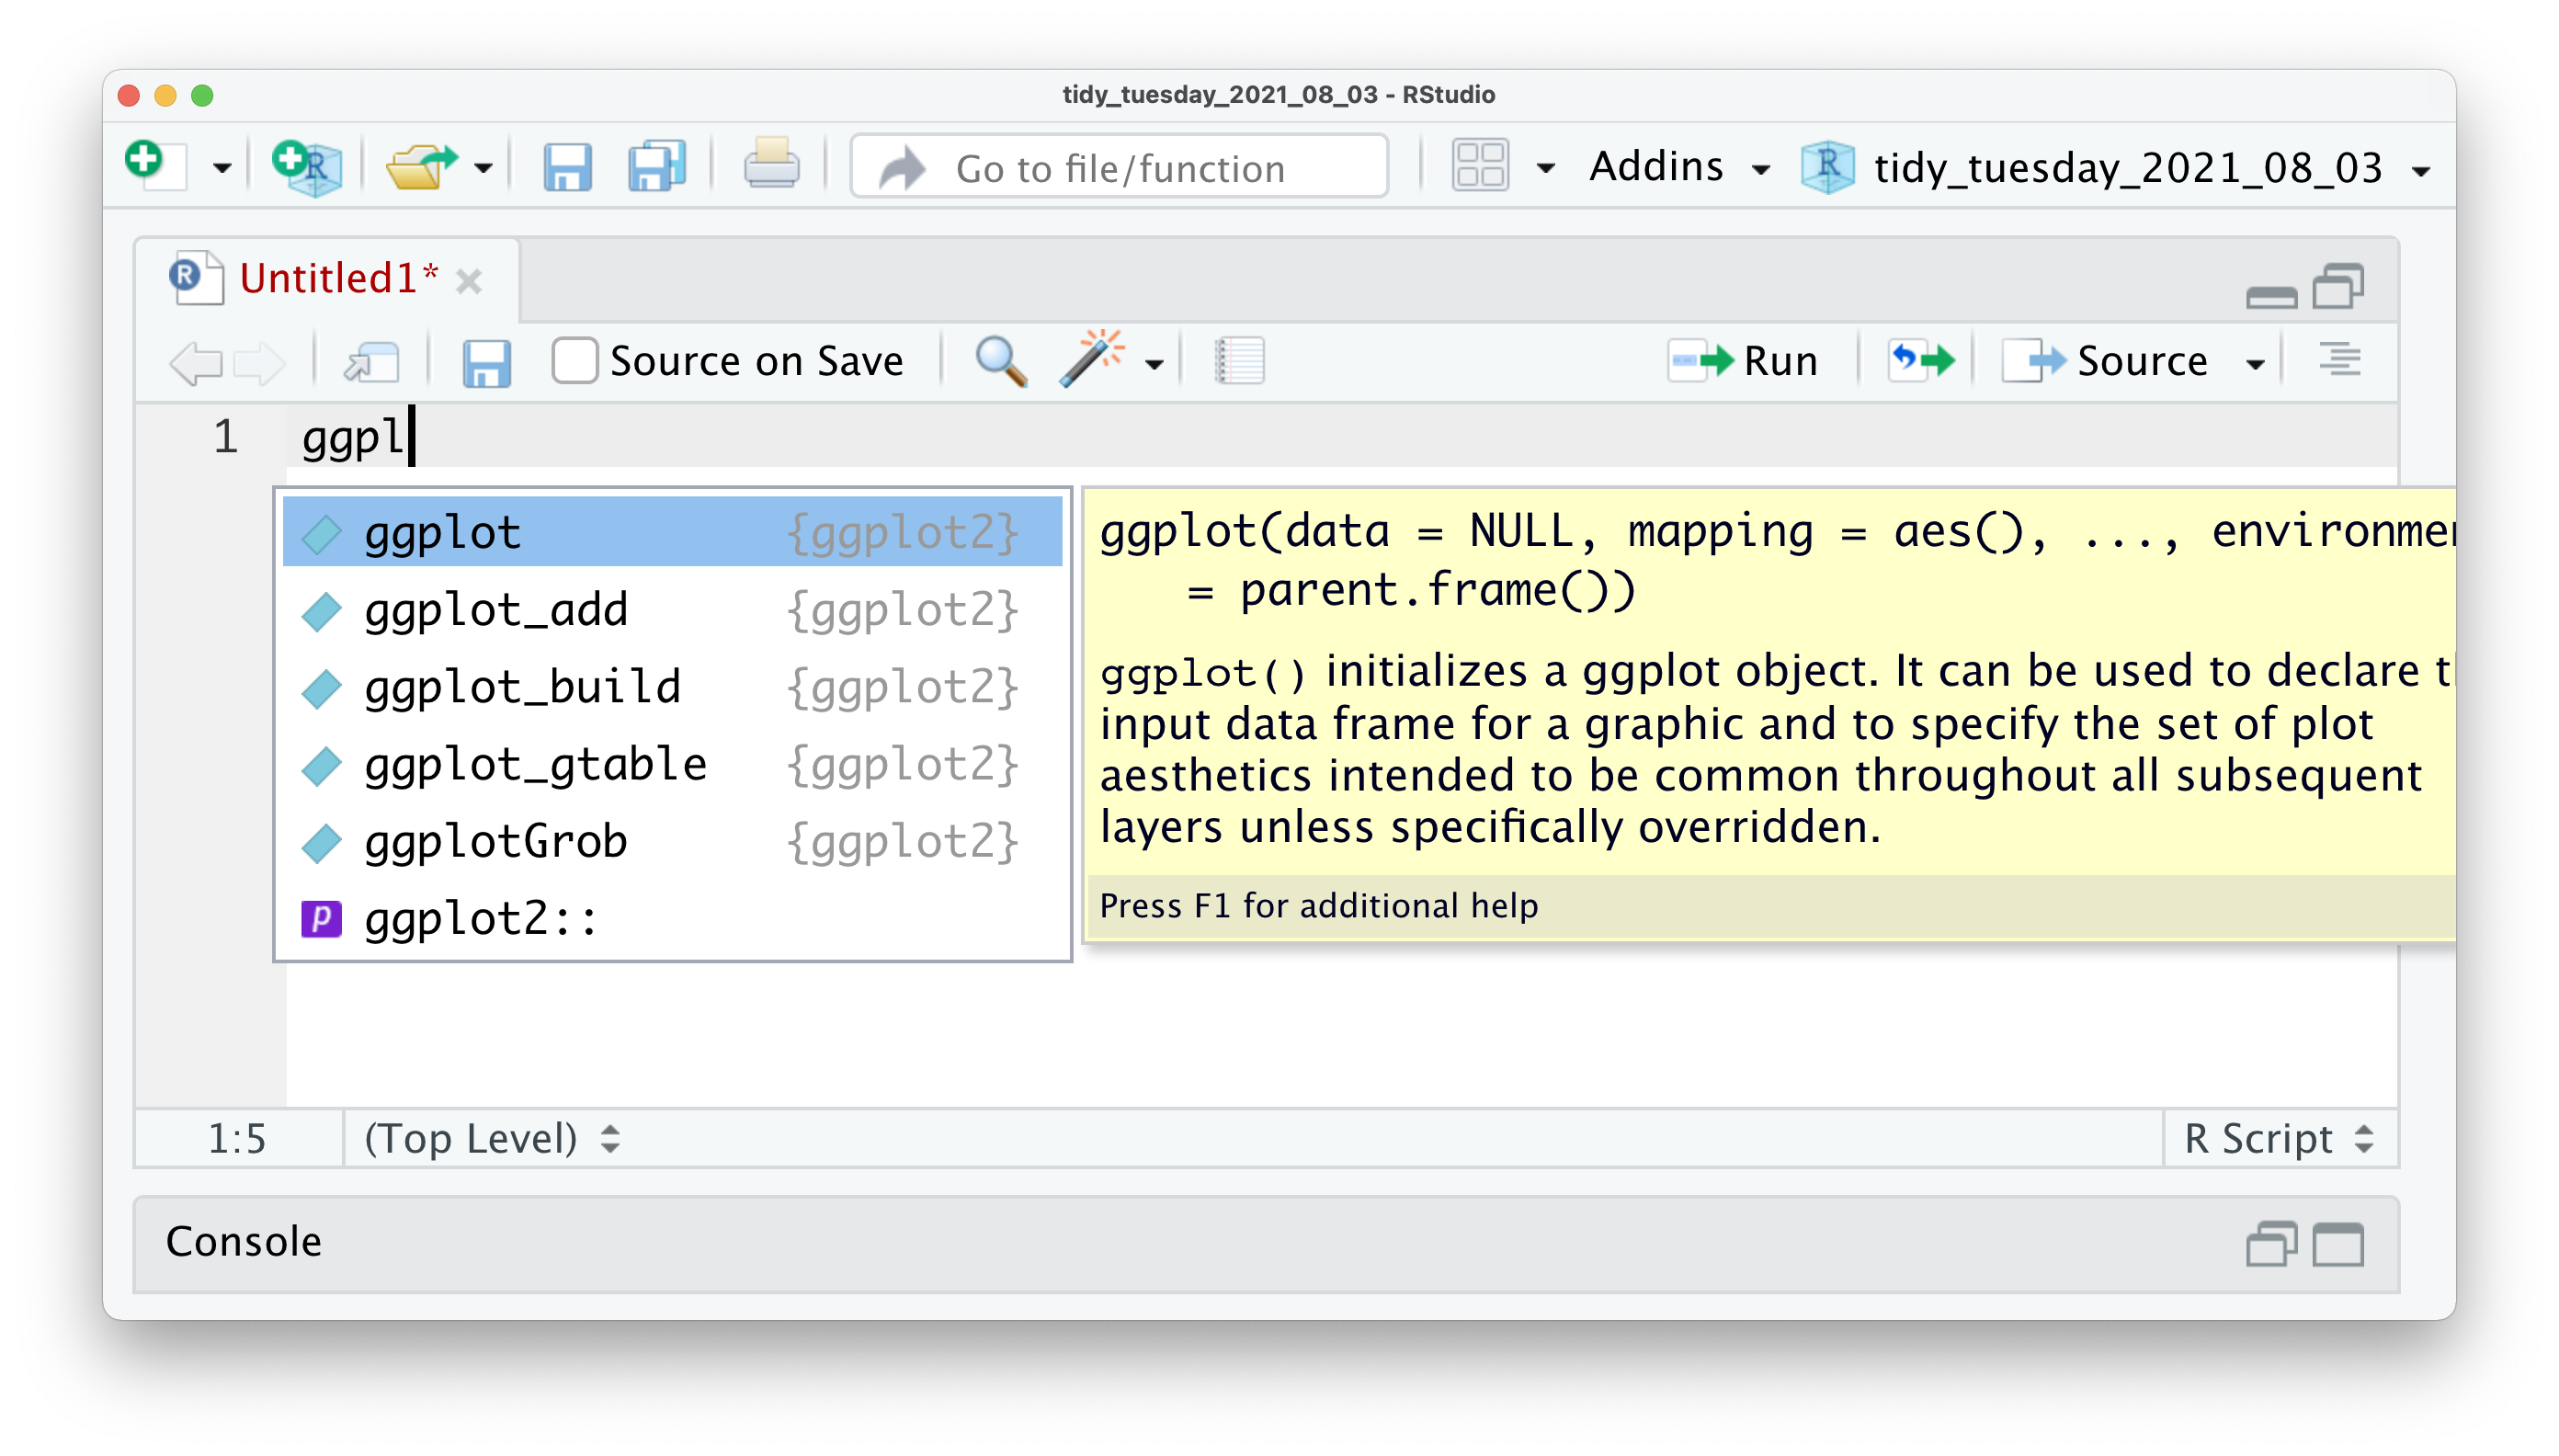
\includegraphics{images/chapter_06_img/02_r_script/02_r_script_code_completion.png}

Not only does RStudio show you all the available options, but it also
tells you which package this function is from. In this case, all listed
functions are from the \texttt{ggplot2} package. Furthermore, when you
select one of the options but have not pressed \texttt{Return} yet, you
also get to see a yellow box, which provides you with a quick reference
of all the arguments that this function accepts. So you do not have to
memorise all the functions and their arguments.

\section{\texorpdfstring{Using
\emph{Quarto}}{Using Quarto}}\label{sec-r-markdown-and-r-notebooks}

There is too much to say about \emph{Quarto}, which is why I only will
highlight that it exists and point out the one feature that might
convince you to choose this format over plain \emph{R} scripts: They
look like a Word document (almost).

The predecessor of \emph{Quarto} was called \emph{R} Markdown, which is
a combination of \emph{R} and '\emph{Markdown'}. \emph{`Markdown'} is a
way of writing and formatting text documents without needing software
like MS Word. Instead, you write everything in plain text. Such plain
text can be converted into many different document types such as HTML
websites, PDF or Word documents. If you would like to see how it works,
I recommend looking at the~\hyperref[0]{Quarto Website}. To create a
\emph{Quarto} file, click on
\texttt{File\ \textgreater{}\ New\ File\ \textgreater{}\ Quarto\ Document...}.

A \emph{Quarto} file works oppositely to an \emph{R} script. By default,
an \emph{R} script considers everything as code and only through
commenting \texttt{\#} we can include text to describe what the code
does. This is what you have seen in all the coding examples so far. On
the other hand, a \emph{Quarto} file considers everything as text, and
we have to specify what is code. We can do so by inserting \emph{`code
chunks'}. Therefore, there is less of a need to use comments \texttt{\#}
in \emph{Quarto} files because you can write about it like you would in
MS Word. Another convenience of \emph{Quarto} files is that results from
your analysis are immediately shown underneath the code chunk and not in
the console.

\includegraphics{images/chapter_06_img/03_r_markdown/01_quarto_plain.png}

If you switch your view to the \texttt{Visual\ Editor} it almost looks
like you are writing a report in MS Word. In order to switch to the
\texttt{Visual\ Editor} you need to either click on \texttt{Visual} in
the top left or click on the gear icon and select
\texttt{Use\ Visual\ Editor}.

\includegraphics{images/chapter_06_img/03_r_markdown/02_quarto_visual_editor_menu.png}

\includegraphics{images/chapter_06_img/03_r_markdown/03_quarto_visual_editor.png}

So, when should you use an \emph{R} script, and when should you use
\emph{Quarto}. The rule-of-thumb is that if you intend to write a
report, assignment, thesis or another form of publication, it might be
better to work in a \emph{Quarto} file. If this does not apply, you
might want to use an \emph{R} Script. As mentioned above, \emph{Quarto}
files emphasise writing about your analysis, while \emph{R} scripts
primarily focus on code. In my projects, I often have a mixture of both.
I use \emph{R} Scripts to carry out data wrangling and my primary
analysis and then use \emph{Quarto} files to present the findings,
e.g.~creating plots, tables, and other components of a report. By the
way, this book is written in \emph{Quarto}.

No matter your choice, it will neither benefit nor disadvantage you in
your \emph{R} journey or when working through this book. The choice is
all yours. You will likely come to appreciate both formats for what they
offer.

\bookmarksetup{startatroot}

\chapter{Data Wrangling}\label{sec-data-wrangling}

\begin{quote}
\textbf{Data wrangling} --- also called~\textbf{data
cleaning},~\textbf{data remediation}, or~\textbf{data munging}---refers
to a variety of processes designed to transform raw data into more
readily used formats. The exact methods differ from project to project
depending on the data you're leveraging and the goal you're trying to
achieve. (Stobierski 2021)
\end{quote}

You collected your data over months (and sometimes years), and all you
want to know is whether your data makes sense and reveals something
nobody would have ever expected. However, before we can truly go ahead
with our analysis, it is essential to understand whether our data is
`tidy'. What I mean is that our data is at the quality we would expect
it to be and can be reliably used for data analysis. After all, the
results of our research are only as good as our data and the methods we
deploy to achieve the desired insights.

Very often, the data we receive is everything else but clean, and we
need to check whether our data is fit for analysis and ensure it is in a
format that is easy to handle. For small datasets, this is usually a
brief exercise. However, I found myself cleaning data for a month
because the dataset was spread out into multiple spreadsheets with
different numbers of columns and odd column names that were not
consistent. Thus, data wrangling is an essential first step in any data
analysis. It is a step that cannot be skipped and has to be performed on
every new dataset. If your background is in qualitative research, you
likely conducted interviews which you had to transcribe. The process of
creating transcriptions is comparable to data wrangling in quantitative
datasets - and equally tedious.

Luckily, \emph{R} provides many useful functions to make our lives
easier. You will be in for a treat if you are like me and used to do
this in Excel. It is a lot simpler using \emph{R} to achieve a clean
dataset.

Here is an overview of the different steps we usually work through
before starting with our primary analysis. This list is certainly not
exhaustive:

\begin{itemize}
\item
  Import data,
\item
  Check data types,
\item
  Recode and arrange factors, i.e.~categorical data, and
\item
  Run missing data diagnostics.
\end{itemize}

\section{Import your data}\label{sec-import-your-data}

The \texttt{r4np} package hosts several different datasets to work with,
but at some point, you might want to apply your \emph{R} knowledge to
your own data. Therefore, an essential first step is to import your data
into RStudio. There are three different methods, all of which are very
handy:

\begin{enumerate}
\def\labelenumi{\arabic{enumi}.}
\item
  Click on your data file in the \emph{Files} pane and choose
  \texttt{Import\ Dataset}.
\item
  Use the \texttt{Import\ Dataset} button in the \emph{Environment}
  pane.
\item
  Import your data calling one of the \texttt{readr} functions in the
  \emph{Console} or \emph{R} script.
\end{enumerate}

We will use the \texttt{readr} package for all three options. Using this
package we can import a range of different file formats, including
\texttt{.csv}, \texttt{.tsv}, \texttt{.txt}. If you want to import data
from an \texttt{.xlsx} file, you need to use another package called
\texttt{readxl}. Similarly, if you used SPSS, Stata or SAS files before
and want to use them in \emph{R} you can use the \texttt{haven} package.
The following sections will primarily focus on using \texttt{readr} via
RStudio or directly in your \emph{Console} or \emph{R} script.

\subsection{\texorpdfstring{Import data from the \emph{Files}
pane}{Import data from the Files pane}}\label{import-data-from-the-files-pane}

This approach is by far the easiest. Let's assume you have a dataset
called \texttt{gender\_age.csv} in your \texttt{00\_raw\_data} folder.
If you wish to import it, you can do the following:

\begin{enumerate}
\def\labelenumi{\arabic{enumi}.}
\item
  Click on the name of the file.
\item
  Select \texttt{Import\ Dataset}.
\end{enumerate}

\includegraphics{images/chapter_07_img/01_files_pane_import/01_files_pane_import.png}

\begin{enumerate}
\def\labelenumi{\arabic{enumi}.}
\setcounter{enumi}{2}
\tightlist
\item
  A new window will open, and you can choose different options. You also
  see a little preview of how the data looks like. This is great if you
  are not sure whether you did it correctly.
\end{enumerate}

\includegraphics{images/chapter_07_img/01_files_pane_import/02_files_pane_import.png}

\begin{enumerate}
\def\labelenumi{\arabic{enumi}.}
\setcounter{enumi}{3}
\item
  You can change how data should be imported, but the default should be
  fine in most cases. Here is a quick breakdown of the most important
  options:

  \begin{itemize}
  \item
    \texttt{Name} allows you to change the object name, i.e.~the name of
    the object this data will be assigned to. I often use
    \texttt{df\_raw} (\texttt{df} stand for \texttt{data\ frame}, which
    is how \emph{R} calls such rectangular datasets).
  \item
    \texttt{Skip} is helpful if your data file starts with several empty
    rows at the top. You can remove them here.
  \item
    \texttt{First\ Row\ as\ Names} is ticked by default. In most Social
    Science projects, we tend to have the name of the variables as the
    first row in our dataset.
  \item
    \texttt{Trim\ Spaces} removes any unnecessary whitespace in your
    dataset. Leave it ticked.
  \item
    \texttt{Open\ Data\ Viewer} allows you to look at your imported
    dataset. I use it rarely, but it can be helpful at times.
  \item
    \texttt{Delimiter} defines how your columns are separated from each
    other in your file. If it is a \texttt{.csv} file, it would imply it
    is a `comma-separated value', i.e.~\texttt{,}. This setting can be
    changed for different files, depending on how your data is
    delimited. You can even use the option \texttt{Other…} to specify a
    custom separation option.
  \item
    \texttt{NA} specifies how missing values in your data are
    acknowledged. By default, empty cells in your data will be
    recognised as missing data.
  \end{itemize}
\end{enumerate}

\includegraphics{images/chapter_07_img/01_files_pane_import/03_files_pane_import.png}

\begin{enumerate}
\def\labelenumi{\arabic{enumi}.}
\setcounter{enumi}{4}
\item
  Once you are happy with your choices, you can click on
  \texttt{Import}.
\item
  You will find your dataset in the \emph{Environment} pane.
\end{enumerate}

\includegraphics{images/chapter_07_img/01_files_pane_import/04_files_pane_import.png}

In the \emph{Console}, you can see that \emph{R} also provides the
\texttt{Column\ specification}, which we need later when inspecting
`data types'. \texttt{readr} automatically imports all text-based
columns as \texttt{chr}, i.e.~\texttt{character} values. However, this
might not always be the correct data type. We will cover more of this
aspect of data wrangling in Section~\ref{sec-change-data-types}.

\subsection{\texorpdfstring{Importing data from the \emph{Environment}
pane}{Importing data from the Environment pane}}\label{sec-importing-data-from-the-environment-pane}

The process of importing datasets from the \emph{Environment} pane
follows largely the one from the \emph{Files} pane. Click on
\texttt{Import\ Dataset\ \textgreater{}\ From\ Text\ (readr)…}. The only
main difference lies in having to find the file using the
\texttt{Browse…} button. The rest of the steps are the same as above.

Be aware that you will have to use the \emph{Environment} pane for
importing data from specific file types, e.g.~\texttt{.txt}. The
\emph{File} pane would only open the file but not import the data for
further processing.

\subsection{Importing data using functions
directly}\label{sec-importing-data-using-functions}

If you organised your files well, it could be effortless and quick to
use all the functions from \texttt{readr} directly. Here are two
examples of how you can use \texttt{readr} to import your data. Make
sure you have the package loaded.

\begin{Shaded}
\begin{Highlighting}[]
\CommentTok{\# Import data from \textquotesingle{}.csv\textquotesingle{}}
\FunctionTok{read\_csv}\NormalTok{(}\StringTok{"00\_raw\_data/gender\_age.csv"}\NormalTok{)}

\CommentTok{\# Import data from any text file by defining the separator}
\FunctionTok{read\_delim}\NormalTok{(}\StringTok{"00\_raw\_data/gender\_age.txt"}\NormalTok{, }\AttributeTok{delim =} \StringTok{"|"}\NormalTok{)}
\end{Highlighting}
\end{Shaded}

You might be wondering whether you can use \texttt{read\_delim()} to
import \texttt{.csv} files too. The answer is `Yes, you can!'. In
contrast to \texttt{read\_delim()}, \texttt{read\_csv()} sets the
delimiter to \texttt{,} by default. This is mainly for convenience
because \texttt{.csv} files are one of the most popular file formats
used to store data.

You might also be wondering what a \emph{`delimiter'} is. When you
record data in a plain-text file, it is easy to see where a new
observation starts and ends because it is defined by a row in your file.
However, we also need to tell our software where a new column starts,
i.e.~where a cell begins and ends. Consider the following example. We
have a file that holds our data which looks like this:

\begin{verbatim}
idagegender
124male
256female
333male
\end{verbatim}

The first row we probably can still decipher as \texttt{id},
\texttt{age}, \texttt{gender}. However, the next row makes it difficult
to understand which value represents the \texttt{id} of a participant
and which value reflects the \texttt{age} of that participant. Like us,
computer software would find it hard too to decide on this ambiguous
content. Thus, we need to use delimiters to make it very clear which
value belongs to which column. For example, in a \texttt{.csv} file, the
data would be separated by a \texttt{,}.

\begin{verbatim}
id,age,gender
1,24,male
2,56,female
3,33,male
\end{verbatim}

Considering our example from above, we could also use
\texttt{\textbar{}} as a delimiter, but this is very unusual.

\begin{verbatim}
id|age|gender
1|24|male
2|56|female
3|33|male
\end{verbatim}

An important advantage of this approach is the ability to load large
data files much more quickly. The previous options offer a preview of
your data, but loading this preview can take a long time for large
datasets. Therefore, I highly recommend using the \texttt{readr}
functions directly in the console or your \emph{R} script to avoid
frustration when importing large datasets.

There is a lot more to \texttt{readr} than could be covered in this
book. If you want to know more about this \emph{R} package, I highly
recommend looking at the \href{https://readr.tidyverse.org}{readr
webpage}.

\section{Inspecting your data}\label{sec-inspecting-raw-data}

For the rest of this chapter, we will use the World Value Survery data
(Haerpfer et al. 2022) (\texttt{wvs}) from the \texttt{r4np} package.
However, we do not know much about this dataset, and therefore we cannot
ask any research questions worth investigating. Therefore, we need to
look at what it contains. The first method of inspecting a dataset is to
type the name of the object, i.e.~\texttt{wvs}.

\begin{Shaded}
\begin{Highlighting}[]
\CommentTok{\# Ensure you loaded the \textquotesingle{}r4np\textquotesingle{} package first}
\FunctionTok{library}\NormalTok{(r4np)}

\CommentTok{\# Show the data in the console}
\NormalTok{wvs}
\end{Highlighting}
\end{Shaded}

\begin{verbatim}
# A tibble: 8,564 x 7
   `Participant ID` `Country name`    Gender   Age relationship_status
              <dbl> <chr>              <dbl> <dbl> <chr>              
 1         68070001 Bolivia, Plurina~      0    60 married            
 2         68070002 Bolivia, Plurina~      0    40 married            
 3         68070003 Bolivia, Plurina~      0    25 single             
 4         68070004 Bolivia, Plurina~      1    71 widowed            
 5         68070005 Bolivia, Plurina~      1    38 married            
 6         68070006 Bolivia, Plurina~      1    20 separated          
 7         68070007 Bolivia, Plurina~      0    39 single             
 8         68070008 Bolivia, Plurina~      1    19 single             
 9         68070009 Bolivia, Plurina~      0    20 single             
10         68070010 Bolivia, Plurina~      1    37 married            
# i 8,554 more rows
# i 2 more variables: Freedom.of.Choice <dbl>,
#   `Satisfaction-with-life` <dbl>
\end{verbatim}

The result is a series of rows and columns. The first information we
receive is: \texttt{A\ tibble:\ 69,578\ x\ 7}. This indicates that our
dataset has 69,578 observations (i.e.~rows) and 9 columns
(i.e.~variables). This rectangular format is the one we encounter most
frequently in Social Sciences (and probably beyond). If you ever worked
in Microsoft Excel, this format will look familiar. However, rectangular
data is not necessarily \texttt{tidy} data. Wickham (2014) (p.~4)
defines tidy data as follows:

\begin{quote}
\begin{enumerate}
\def\labelenumi{\arabic{enumi}.}
\tightlist
\item
  Each variable forms a column.
\item
  Each observation forms a row.
\item
  Each type of observational unit forms a table.
\end{enumerate}
\end{quote}

Even though it might be nice to look at a tibble in the console, it is
not particularly useful. Depending on your monitor size, you might only
see a small number of columns, and therefore we do not get to see a
complete list of all variables. In short, we hardly ever will find much
use in inspecting data this way. Luckily other functions can help us.

If you want to see each variable covered in the dataset and their data
types, you can use the function \texttt{glimpse()} from the
\texttt{dplyr} package which is loaded as part of the \texttt{tidyverse}
package.

\begin{Shaded}
\begin{Highlighting}[]
\FunctionTok{glimpse}\NormalTok{(wvs)}
\end{Highlighting}
\end{Shaded}

\begin{verbatim}
Rows: 5
Columns: 7
$ `Participant ID`         <dbl> 68070001, 68070002, 68070003, 68070~
$ `Country name`           <chr> "Bolivia, Plurinational State of", ~
$ Gender                   <dbl> 0, 0, 0, 1, 1
$ Age                      <dbl> 60, 40, 25, 71, 38
$ relationship_status      <chr> "married", "married", "single", "wi~
$ Freedom.of.Choice        <dbl> 7, 8, 10, 5, 5
$ `Satisfaction-with-life` <dbl> 5, 7, 8, 5, 7
\end{verbatim}

The output of glimpse shows us the name of each column/variable after
the \texttt{\$}, for example,
\texttt{\textasciigrave{}Participant\ ID\textasciigrave{}}. The
\texttt{\$} is used to lookup certain variables in our dataset. For
example, if we want to inspect the column \texttt{relationship\_status}
only, we could write the following:

\begin{Shaded}
\begin{Highlighting}[]
\NormalTok{wvs}\SpecialCharTok{$}\NormalTok{relationship\_status}
\end{Highlighting}
\end{Shaded}

\begin{verbatim}
   [1] "married"                    "married"                   
   [3] "single"                     "widowed"                   
   [5] "married"                    "separated"                 
   [7] "single"                     "single"                    
....
\end{verbatim}

When using \texttt{glimpse()} we find the recognised data type for each
column, i.e.~each variable, in \texttt{\textless{}...\textgreater{}},
for example \texttt{\textless{}chr\textgreater{}}. We will return to
data types in Section~\ref{sec-change-data-types}. Lastly, we get
examples of the values included in each variable. This output is much
more helpful.

I use \texttt{glimpse()} very frequently for different purposes, for
example:

\begin{itemize}
\item
  to understand what variables are included in a dataset,
\item
  to check the correctness of data types,
\item
  to inspect variable names for typos or unconventional names,
\item
  to look up variable names.
\end{itemize}

There is one more way to inspect your data and receive more information
about it by using a specialised \emph{R} package. The \texttt{skimr}
package is excellent in `skimming' your dataset. It provides not only
information about variable names and data types but also provides some
descriptive statistics. If you installed the \texttt{r4np} package and
called the function \texttt{install\_r4np()}, you will have
\texttt{skimr} installed already.

\begin{Shaded}
\begin{Highlighting}[]
\NormalTok{skimr}\SpecialCharTok{::}\FunctionTok{skim}\NormalTok{(wvs)}
\end{Highlighting}
\end{Shaded}

The output in the \emph{Console} should look like this:

\includegraphics{images/chapter_07_img/02_skimr_output/skimr_output.png}

As you can tell, there is a lot more information in this output. Many
descriptive statistics that could be useful are already displayed.
\texttt{skim()} provides a summary of the dataset and then automatically
sorts the variables by data type. Depending on the data type, you also
receive different descriptive statistics. As a bonus, the function also
provides a histogram for numeric variables. However, there is one main
problem: Some of the numeric variables are not numeric:
\texttt{Participant\ ID} and \texttt{Gender}. Thus, we will have to
correct the data types in a moment.

Inspecting your data in this way can be helpful to get a better
understanding of what your data includes and spot problems with it. In
addition, if you receive data from someone else, these methods are an
excellent way to familiarise yourself with the dataset relatively
quickly. Since I prepared this particular dataset for this book, I also
made sure to provide documentation for it. You can access it by using
\texttt{?wvs} in the \emph{Console}. This will open the documentation in
the \emph{Help} pane. Such documentation is available for every dataset
we use in this book.

\section{\texorpdfstring{Cleaning your column names: Call the
\texttt{janitor}}{Cleaning your column names: Call the janitor}}\label{sec-colnames-cleaning}

If you have eagle eyes, you might have noticed that most of the variable
names in \texttt{wvs} are not consistent or easy to read/use.

\phantomsection\label{messy_column_names}%
\begin{Shaded}
\begin{Highlighting}[]
\CommentTok{\# Whitespace and inconsistent capitalisation}
\NormalTok{Participant ID        }
\NormalTok{Country name          }
\NormalTok{Gender                }
\NormalTok{Age                   }

\CommentTok{\# Difficult to read}
\NormalTok{Freedom.of.Choice     }
\NormalTok{Satisfaction}\SpecialCharTok{{-}}\NormalTok{with}\SpecialCharTok{{-}}\NormalTok{life}
\end{Highlighting}
\end{Shaded}

From Section~\ref{sec-coding-etiquette}, you will remember that being
consistent in writing your code and naming your objects is essential.
The same applies, of course, to variable names. \emph{R} will not break
using the existing names, but it will save you a lot of frustration if
we take a minute to clean the names and make them more consistent. Since
we will use column names in almost every line of code we produce, it is
best to standardise them and make them easier to read and write.

You are probably thinking: ``This is easy. I just open the dataset in
Excel and change all the column names.'' Indeed, it would be a viable
and easy option, but it is not very efficient, especially with larger
datasets with many more variables. Instead, we can make use of the
\texttt{janitor} package. By definition, \texttt{janitor} is a package
that helps to clean up whatever needs cleaning. In our case, we want to
tidy our column names. We can use the function \texttt{clean\_names()}
to achieve this. We store the result in a new object called \texttt{wvs}
to keep those changes. The object will also show up in our
\emph{Environment} pane.

\begin{Shaded}
\begin{Highlighting}[]
\NormalTok{wvs\_clean }\OtherTok{\textless{}{-}}\NormalTok{ janitor}\SpecialCharTok{::}\FunctionTok{clean\_names}\NormalTok{(wvs)}

\FunctionTok{glimpse}\NormalTok{(wvs\_clean)}
\end{Highlighting}
\end{Shaded}

\begin{verbatim}
Rows: 8,564
Columns: 7
$ participant_id         <dbl> 68070001, 68070002, 68070003, 6807000~
$ country_name           <chr> "Bolivia, Plurinational State of", "B~
$ gender                 <dbl> 0, 0, 0, 1, 1, 1, 0, 1, 0, 1, 1, 1, 1~
$ age                    <dbl> 60, 40, 25, 71, 38, 20, 39, 19, 20, 3~
$ relationship_status    <chr> "married", "married", "single", "wido~
$ freedom_of_choice      <dbl> 7, 8, 10, 5, 5, 5, 5, 10, 6, 9, 5, 8,~
$ satisfaction_with_life <dbl> 5, 7, 8, 5, 7, 3, 3, 8, 7, 8, 9, 6, 7~
\end{verbatim}

Now that \texttt{janitor} has done its magic, we suddenly have easy to
read variable names that are consistent with the \emph{`Tidyverse style
guide'} (Wickham 2021).

If, for whatever reason, the variable names are still not looking the
way you want, you can use the function \texttt{rename()} from the
\texttt{dplyr} package to manually assign new variable names.

\begin{Shaded}
\begin{Highlighting}[]
\NormalTok{wvs\_clean }\OtherTok{\textless{}{-}} 
\NormalTok{  wvs\_clean }\SpecialCharTok{|\textgreater{}}
  \FunctionTok{rename}\NormalTok{(}\AttributeTok{satisfaction =}\NormalTok{ satisfaction\_with\_life,}
         \AttributeTok{country =}\NormalTok{ country\_name)}

\FunctionTok{glimpse}\NormalTok{(wvs\_clean)}
\end{Highlighting}
\end{Shaded}

\begin{verbatim}
Rows: 8,564
Columns: 7
$ participant_id      <dbl> 68070001, 68070002, 68070003, 68070004, ~
$ country             <chr> "Bolivia, Plurinational State of", "Boli~
$ gender              <dbl> 0, 0, 0, 1, 1, 1, 0, 1, 0, 1, 1, 1, 1, 0~
$ age                 <dbl> 60, 40, 25, 71, 38, 20, 39, 19, 20, 37, ~
$ relationship_status <chr> "married", "married", "single", "widowed~
$ freedom_of_choice   <dbl> 7, 8, 10, 5, 5, 5, 5, 10, 6, 9, 5, 8, 8,~
$ satisfaction        <dbl> 5, 7, 8, 5, 7, 3, 3, 8, 7, 8, 9, 6, 7, 7~
\end{verbatim}

You are probably wondering what \texttt{\textbar{}\textgreater{}} stands
for. This symbol is called a \emph{`piping operator'} , and it allows us
to chain multiple functions together by considering the output of the
previous function. So, do not confuse \texttt{\textless{}-} with
\texttt{\textbar{}\textgreater{}}. Each operator serves a different
purpose. The \texttt{\textbar{}\textgreater{}} has become synonymous
with the \texttt{tidyverse} approach to \emph{R} programming and is the
chosen approach for this book. Many functions from the
\texttt{tidyverse} are designed to be chained together.

If we wanted to spell out what we just did, we could say:

\begin{enumerate}
\def\labelenumi{\arabic{enumi}.}
\item
  \texttt{wvs\_clean\ \textless{}-}: We assigned whatever happened to
  the right of the assignment operator to the object
  \texttt{wvs\_clean}.
\item
  \texttt{wvs\_clean\ \textbar{}\textgreater{}}: We defined the dataset
  we want to use with the functions defined after the
  \texttt{\textbar{}\textgreater{}}.
\item
  \texttt{rename(satisfaction\ =\ satisfaction\_with\_life)}: We define
  a new name \texttt{satisfaction} for the column
  \texttt{satisfaction\_with\_life}. Notice that the order is
  \texttt{new\_name\ =\ old\_name}. Here, we also use \texttt{=}. A rare
  occasion where it makes sense to do so.
\end{enumerate}

Just for clarification, the following two lines of code accomplish the
same task. The only difference is that with
\texttt{\textbar{}\textgreater{}} we could chain another function right
after it. So, you could say, it is a matter of taste which approach you
prefer. However, in later chapters, it will become apparent why using
\texttt{\textbar{}\textgreater{}} is very advantageous.

\begin{Shaded}
\begin{Highlighting}[]
\CommentTok{\# Renaming a column using \textquotesingle{}|\textgreater{}\textquotesingle{}}
\NormalTok{wvs\_clean }\SpecialCharTok{|\textgreater{}} \FunctionTok{rename}\NormalTok{(}\AttributeTok{satisfaction\_new =}\NormalTok{ satisfaction)}

\CommentTok{\# Renaming a column without \textquotesingle{}|\textgreater{}\textquotesingle{}}
\FunctionTok{rename}\NormalTok{(wvs\_clean, }\AttributeTok{satisfaction\_new =}\NormalTok{ satisfaction)}
\end{Highlighting}
\end{Shaded}

Since you will be using the pipe operator very frequently, it is a good
idea to remember the keyboard shortcut for it: \texttt{Ctrl+Shift+M} for
PC and \texttt{Cmd+Shift+M} for Mac.

Besides \texttt{\textbar{}\textgreater{}} operator you might also find
that some sources use a different pipe operator
\texttt{\%\textgreater{}\%}. The original \texttt{tidyverse} approach
used \texttt{\%\textgreater{}\%} before \emph{R} introduced their own
pipe operator. In short: You can use both of them if you like, but in
90\% of cases, you probably will be fine using the one that comes
shipped with RStudio by default, i.e.~\texttt{\textbar{}\textgreater{}}.
More and more \emph{R} resources adopt the
\texttt{\textbar{}\textgreater{}} operator and there are only few
situations where \texttt{\%\textgreater{}\%} is preferred. For the
content of this book and the techniques demonstrated here, you can use
both operators interchangeably and the code will work just fine.

\section{Data types: What are they and how can you change
them}\label{sec-change-data-types}

When we inspected our data, I mentioned that some variables do not have
the correct data type. You might be familiar with different data types
by classifying them as:

\begin{itemize}
\item
  \emph{Nominal data}, which is categorical data of no particular order,
\item
  \emph{Ordinal data}, which is categorical data with a defined order,
  and
\item
  \emph{Quantitative data}, which is data that usually is represented by
  numeric values.
\end{itemize}

In \emph{R} we have a slightly different distinction:

\begin{itemize}
\item
  \texttt{character} / \texttt{\textless{}chr\textgreater{}}: Textual
  data, for example the text of a tweet.
\item
  \texttt{factor} / \texttt{\textless{}fct\textgreater{}}: Categorical
  data with a finite number of categories with no particular order.
\item
  \texttt{ordered} / \texttt{\textless{}ord\textgreater{}}: Categorical
  data with a finite number of categories with a particular order.
\item
  \texttt{double} / \texttt{\textless{}dbl\textgreater{}}: Numerical
  data with decimal places.
\item
  \texttt{integer} / \texttt{\textless{}int\textgreater{}}: Numerical
  data with whole numbers only (i.e.~no decimals).
\item
  \texttt{logical} / \texttt{\textless{}lgl\textgreater{}}: Logical
  data, which only consists of values \texttt{TRUE} and \texttt{FALSE}.
\item
  \texttt{date} / \texttt{date}: Data which consists of dates,
  e.g.~\texttt{2021-08-05}.
\item
  \texttt{date-time} / \texttt{dttm}: Data which consists of dates and
  times, e.g.~\texttt{2021-08-05\ 16:29:25\ BST}.
\end{itemize}

For a complete list of data types, I recommend looking at
\href{https://tibble.tidyverse.org/articles/types.html}{`Column Data
Types'} (Müller and Wickham 2021).

\emph{R} has a fine-grained categorisation of data types. The most
important distinction, though, lies between
\texttt{\textless{}chr\textgreater{}},
\texttt{\textless{}fct\textgreater{}}/\texttt{\textless{}ord\textgreater{}}
and \texttt{\textless{}dbl\textgreater{}} for most datasets in the
Social Sciences. Still, it is good to know what the abbreviations in
your \texttt{tibble} mean and how they might affect your analysis.

Now that we have a solid understanding of different data types, we can
look at our dataset and see whether \texttt{readr} classified our
variables correctly.

\begin{Shaded}
\begin{Highlighting}[]
\FunctionTok{glimpse}\NormalTok{(wvs\_clean)}
\end{Highlighting}
\end{Shaded}

\begin{verbatim}
Rows: 8,564
Columns: 7
$ participant_id      <dbl> 68070001, 68070002, 68070003, 68070004, ~
$ country             <chr> "Bolivia, Plurinational State of", "Boli~
$ gender              <dbl> 0, 0, 0, 1, 1, 1, 0, 1, 0, 1, 1, 1, 1, 0~
$ age                 <dbl> 60, 40, 25, 71, 38, 20, 39, 19, 20, 37, ~
$ relationship_status <chr> "married", "married", "single", "widowed~
$ freedom_of_choice   <dbl> 7, 8, 10, 5, 5, 5, 5, 10, 6, 9, 5, 8, 8,~
$ satisfaction        <dbl> 5, 7, 8, 5, 7, 3, 3, 8, 7, 8, 9, 6, 7, 7~
\end{verbatim}

\texttt{readr} did a great job in identifying all the numeric variables.
However, by default, \texttt{readr} imports all variables that include
text as \texttt{\textless{}chr\textgreater{}}. It appears as if this is
not entirely correct for our dataset. The variables \texttt{country},
\texttt{gender} and \texttt{relationship\_status} specify a finite
number of categories. Therefore they should be classified as a
\texttt{factor}. The variable \texttt{participant\_id} is represented by
numbers, but its meaning is also rather categorical. We would not use
the ID numbers of participants to perform additions or multiplications.
This would make no sense. Therefore, it might be wise to turn them into
a \texttt{factor}, even though we likely will not use it in our analysis
and would make no difference. However, I am a stickler for those kinds
of things.

To perform the conversion, we need to use two new functions from
\texttt{dplyr}:

\begin{itemize}
\item
  \texttt{mutate()}: Changes, i.e.~`mutates', a variable.
\item
  \texttt{as\_factor()}: Converts data from one type into a
  \texttt{factor}.
\end{itemize}

If we want to convert all variables in one go, we can put them into the
same function, separated by a \texttt{,}.

\begin{Shaded}
\begin{Highlighting}[]
\NormalTok{wvs\_clean }\OtherTok{\textless{}{-}}
\NormalTok{  wvs\_clean }\SpecialCharTok{|\textgreater{}}
  \FunctionTok{mutate}\NormalTok{(}\AttributeTok{country =} \FunctionTok{as\_factor}\NormalTok{(country),}
         \AttributeTok{gender =} \FunctionTok{as\_factor}\NormalTok{(gender),}
         \AttributeTok{relationship\_status =} \FunctionTok{as\_factor}\NormalTok{(relationship\_status),}
         \AttributeTok{participant\_id =} \FunctionTok{as\_factor}\NormalTok{(participant\_id)}
\NormalTok{         )}

\FunctionTok{glimpse}\NormalTok{(wvs\_clean)}
\end{Highlighting}
\end{Shaded}

\begin{verbatim}
Rows: 8,564
Columns: 7
$ participant_id      <fct> 68070001, 68070002, 68070003, 68070004, ~
$ country             <fct> "Bolivia, Plurinational State of", "Boli~
$ gender              <fct> 0, 0, 0, 1, 1, 1, 0, 1, 0, 1, 1, 1, 1, 0~
$ age                 <dbl> 60, 40, 25, 71, 38, 20, 39, 19, 20, 37, ~
$ relationship_status <fct> married, married, single, widowed, marri~
$ freedom_of_choice   <dbl> 7, 8, 10, 5, 5, 5, 5, 10, 6, 9, 5, 8, 8,~
$ satisfaction        <dbl> 5, 7, 8, 5, 7, 3, 3, 8, 7, 8, 9, 6, 7, 7~
\end{verbatim}

The output in the console shows that we successfully performed the
transformation and our data types are as we intended them to be. Mission
accomplished.

If you need to convert all \texttt{\textless{}chr\textgreater{}} columns
you can use \texttt{mutate\_if(is.character,\ as\_factor)} instead. This
function will look at each column and if it is a \texttt{character} type
variable, it will convert it into a \texttt{factor}. However, use this
function only if you are certain that all \texttt{character} columns
need converting. If this is the case, it can be a huge time-saver. Here
is the corresponding code snippet:

\begin{Shaded}
\begin{Highlighting}[]
\NormalTok{wvs\_clean }\SpecialCharTok{|\textgreater{}}
  \FunctionTok{mutate\_if}\NormalTok{(is.character, as\_factor)}
\end{Highlighting}
\end{Shaded}

Lastly, there might be occasions where you want to convert data into
other formats than from \texttt{\textless{}chr\textgreater{}} to
\texttt{\textless{}fct\textgreater{}}. Similar to \texttt{as\_factor()}
there are more functions available to transform your data into the
correct format of your choice:

\begin{itemize}
\item
  \texttt{as.integer()}: Converts values into integers, i.e.~without
  decimal places. Be aware that this function does not round values as
  you might expect. Instead, it removes any decimals as if they never
  existed.
\item
  \texttt{as.numeric()}: Converts values into numbers with decimals if
  they are present.
\item
  \texttt{as.character()}: Converts values to string values, even if
  they are numbers. If you use \texttt{readr} to import your data, you
  will not often use this function because \texttt{readr} imports
  unknown data types as \texttt{\textless{}chr\textgreater{}} by
  default.
\end{itemize}

All these functions can be used in the same way as we did before. Here
are three examples illustrating their use.

\begin{Shaded}
\begin{Highlighting}[]
\CommentTok{\# Conversion to character values}
\NormalTok{converted\_data }\OtherTok{\textless{}{-}}
\NormalTok{  wvs\_clean }\SpecialCharTok{|\textgreater{}}
  \FunctionTok{mutate}\NormalTok{(}\AttributeTok{participant\_id =} \FunctionTok{as.character}\NormalTok{(participant\_id),}
         \AttributeTok{age =} \FunctionTok{as.character}\NormalTok{(age))}

\FunctionTok{glimpse}\NormalTok{(converted\_data)}
\end{Highlighting}
\end{Shaded}

\begin{verbatim}
Rows: 8,564
Columns: 7
$ participant_id      <chr> "68070001", "68070002", "68070003", "680~
$ country             <fct> "Bolivia, Plurinational State of", "Boli~
$ gender              <fct> 0, 0, 0, 1, 1, 1, 0, 1, 0, 1, 1, 1, 1, 0~
$ age                 <chr> "60", "40", "25", "71", "38", "20", "39"~
$ relationship_status <fct> married, married, single, widowed, marri~
$ freedom_of_choice   <dbl> 7, 8, 10, 5, 5, 5, 5, 10, 6, 9, 5, 8, 8,~
$ satisfaction        <dbl> 5, 7, 8, 5, 7, 3, 3, 8, 7, 8, 9, 6, 7, 7~
\end{verbatim}

\begin{Shaded}
\begin{Highlighting}[]
\CommentTok{\# Conversion to numeric values}
\NormalTok{converted\_data }\SpecialCharTok{|\textgreater{}}
  \FunctionTok{mutate}\NormalTok{(}\AttributeTok{age =} \FunctionTok{as.numeric}\NormalTok{(age))}
\end{Highlighting}
\end{Shaded}

\begin{verbatim}
# A tibble: 8,564 x 7
   participant_id country             gender   age relationship_status
   <chr>          <fct>               <fct>  <dbl> <fct>              
 1 68070001       Bolivia, Plurinati~ 0         60 married            
 2 68070002       Bolivia, Plurinati~ 0         40 married            
 3 68070003       Bolivia, Plurinati~ 0         25 single             
 4 68070004       Bolivia, Plurinati~ 1         71 widowed            
 5 68070005       Bolivia, Plurinati~ 1         38 married            
 6 68070006       Bolivia, Plurinati~ 1         20 separated          
 7 68070007       Bolivia, Plurinati~ 0         39 single             
 8 68070008       Bolivia, Plurinati~ 1         19 single             
 9 68070009       Bolivia, Plurinati~ 0         20 single             
10 68070010       Bolivia, Plurinati~ 1         37 married            
# i 8,554 more rows
# i 2 more variables: freedom_of_choice <dbl>, satisfaction <dbl>
\end{verbatim}

\begin{Shaded}
\begin{Highlighting}[]
\CommentTok{\# Convert numeric values to integers}
\NormalTok{numeric\_values }\OtherTok{\textless{}{-}} \FunctionTok{tibble}\NormalTok{(}\AttributeTok{values =} \FunctionTok{c}\NormalTok{(}\FloatTok{1.3}\NormalTok{, }\FloatTok{2.6}\NormalTok{, }\FloatTok{3.8}\NormalTok{))}

\NormalTok{numeric\_values }\SpecialCharTok{|\textgreater{}}
  \FunctionTok{mutate}\NormalTok{(}\AttributeTok{integers =} \FunctionTok{as.integer}\NormalTok{(values))}
\end{Highlighting}
\end{Shaded}

\begin{verbatim}
# A tibble: 3 x 2
  values integers
   <dbl>    <int>
1    1.3        1
2    2.6        2
3    3.8        3
\end{verbatim}

\section{Handling factors}\label{sec-handling-factors}

Factors are an essential way to classify observations in our data in
different ways. In terms of data wrangling, there are usually at least
three steps we take to prepare them for analysis:

\begin{itemize}
\tightlist
\item
  Recoding factors,
\item
  Reordering factor levels, and
\item
  Removing factor levels
\end{itemize}

\subsection{Recoding factors}\label{sec-recoding-factors}

Another common problem we have to tackle when working with data is their
representation in the dataset. For example, \texttt{gender} could be
measured as \texttt{male} and \texttt{female}\footnote{A sophisticated
  research project would likely not rely on a dichotomous approach to
  gender, but appreciate the diversity in this regard.} or as \texttt{0}
and \texttt{1}. \emph{R} does not mind which way you represent your
data, but some other software does. Therefore, when we import data from
somewhere else, the values of a variable might not look the way we want.
The practicality of having your data represented accurately as what they
are, becomes apparent when you intend to create tables and plots.

For example, we might be interested in knowing how many participants in
\texttt{wvs\_clean} were \texttt{male} and \texttt{female}. The function
\texttt{count()} from \texttt{dplyr} does precisely that. We can sort
the results, i.e.~\texttt{n}, in descending order by including
\texttt{sort\ =\ TRUE}. By default, \texttt{count()} arranges our
variable \texttt{gender} in alphabetical order.

\begin{Shaded}
\begin{Highlighting}[]
\NormalTok{wvs\_clean }\SpecialCharTok{|\textgreater{}} \FunctionTok{count}\NormalTok{(gender, }\AttributeTok{sort =} \ConstantTok{TRUE}\NormalTok{)}
\end{Highlighting}
\end{Shaded}

\begin{verbatim}
# A tibble: 2 x 2
  gender     n
  <fct>  <int>
1 1       4348
2 0       4216
\end{verbatim}

Now we know how many people were \texttt{male} and \texttt{female} and
how many did not disclose their \texttt{gender}. Or do we? The issue
here is that you would have to know what \texttt{0} and \texttt{1} stand
for. Surely you would have a coding manual that gives you the answer,
but it seems a bit of a complication. For \texttt{gender}, this might
still be easy to remember, but can you recall the ID numbers for 48
countries?

It certainly would be easier to replace the \texttt{0}s and \texttt{1}s
with their corresponding labels. This can be achieved with a simple
function called \texttt{fct\_recode()} from the \texttt{forcats}
\emph{R} package. However, since we `mutate' a variable into something
else, we also have to use the \texttt{mutate()} function.

\begin{Shaded}
\begin{Highlighting}[]
\NormalTok{wvs\_clean }\OtherTok{\textless{}{-}}
\NormalTok{  wvs\_clean }\SpecialCharTok{|\textgreater{}}
  \FunctionTok{mutate}\NormalTok{(}\AttributeTok{gender =} \FunctionTok{fct\_recode}\NormalTok{(gender,}
                             \StringTok{"male"} \OtherTok{=} \StringTok{"0"}\NormalTok{,}
                             \StringTok{"female"} \OtherTok{=} \StringTok{"1"}\NormalTok{))}
\end{Highlighting}
\end{Shaded}

If you have been following along very carefully, you might spot one
oddity in this code: \texttt{"0"} and \texttt{"1"}. You likely recall
that in Chapter~\ref{sec-r-basics-the-very-fundamentals}, I mentioned
that we use \texttt{""} for \texttt{character} values but not for
numbers. So what happens if we run the code and remove \texttt{""}.

\begin{Shaded}
\begin{Highlighting}[]
\NormalTok{wvs\_clean }\SpecialCharTok{|\textgreater{}}
  \FunctionTok{mutate}\NormalTok{(}\AttributeTok{gender =} \FunctionTok{fct\_recode}\NormalTok{(gender,}
                             \StringTok{"male"} \OtherTok{=} \DecValTok{0}\NormalTok{,}
                             \StringTok{"female"} \OtherTok{=} \DecValTok{1}\NormalTok{))}
\end{Highlighting}
\end{Shaded}

\begin{verbatim}
Error in `mutate()`:
i In argument: `gender = fct_recode(gender, male = 0, female =
  1)`.
Caused by error in `fct_recode()`:
! Each element of `...` must be a named string.
i Problems with 2 arguments: male and female
\end{verbatim}

The error message is easy to understand: \texttt{fct\_recode()} only
expects \texttt{strings} as input and not numbers. \emph{R} recognises
\texttt{0} and \texttt{1} as numbers, but \texttt{fct\_recode()} only
converts a \texttt{factor} value into another \texttt{factor} value and
since we `mutated' gender from a \texttt{numeric} variable to a
\texttt{factor} variable, all values of gender are no longer numbers. To
refer to a factor level (i.e.~one of the categories in our factor), we
have to use \texttt{""}. In other words, data types matter and are often
a source of problems with your code. Thus, always pay close attention to
them. For now, it is important to remember that factor levels are always
string values, i.e.~text.

Now that we have change the factor levels to our liking, we can rerun
our analysis and generate a frequency table for \texttt{gender}. This
time we receive a much more readable output.

\begin{Shaded}
\begin{Highlighting}[]
\NormalTok{wvs\_clean }\SpecialCharTok{|\textgreater{}} \FunctionTok{count}\NormalTok{(gender)}
\end{Highlighting}
\end{Shaded}

\begin{verbatim}
# A tibble: 2 x 2
  gender     n
  <fct>  <int>
1 male    4216
2 female  4348
\end{verbatim}

Another benefit of going through the trouble of recoding your factors is
the readability of your plots. For example, we could quickly generate a
bar plot based on the above table and have appropriate labels instead of
\texttt{0} and \texttt{1}.

\begin{Shaded}
\begin{Highlighting}[]
\NormalTok{wvs\_clean }\SpecialCharTok{|\textgreater{}}
  \FunctionTok{count}\NormalTok{(gender) }\SpecialCharTok{|\textgreater{}}
  \FunctionTok{ggplot}\NormalTok{(}\FunctionTok{aes}\NormalTok{(gender, n)) }\SpecialCharTok{+}
  \FunctionTok{geom\_col}\NormalTok{()}
\end{Highlighting}
\end{Shaded}

\begin{figure}[H]

\centering{

\includegraphics{07_data_wrangling_files/figure-pdf/fig-gender-bar-plot-1.pdf}

}

\caption{\label{fig-gender-bar-plot}A bar plot of the factor levels
\texttt{male} and \texttt{female}}

\end{figure}%

Plots are an excellent way to explore your data and understand
relationships between variables. We will learn more about this when we
start to perform analytical steps on our data (see
Chapter~\ref{sec-descriptive-statistics} and beyond).

Another use case for recoding factors could be for purely cosmetic
reasons. For example, when looking through our dataset, we might notice
that some country names are very long and do not look great in data
visualisations or tables. Thus, we could consider shortening them which
is a slightly more advanced process.

First, we need to find out which country names are particularly long.
There are 48 countries in this dataset, so it could take some time to
look through them all. Instead, we could use the function
\texttt{filter()} from \texttt{dplyr} to pick only countries with a long
name. However, this poses another problem: How can we tell the filter
function to pick only country names with a certain length? Ideally, we
would want a function that does the counting for us. As you probably
anticipated, there is a package called \texttt{stringr}, which also
belongs to the \texttt{tidyverse,} and has a function that counts the
number of characters that represent a value in our dataset:
\texttt{str\_length()}. This function takes any \texttt{character}
variable and returns the length of it. This also works with
\texttt{factors} because this function can `coerce' it into a
\texttt{character}, i.e.~it just ignores that it is a \texttt{factor}
and looks at it as if it was a regular \texttt{character} variable. Good
news for us, because now we can put the puzzle pieces together.

\begin{Shaded}
\begin{Highlighting}[]
\NormalTok{wvs\_clean }\SpecialCharTok{|\textgreater{}}
  \FunctionTok{filter}\NormalTok{(}\FunctionTok{str\_length}\NormalTok{(country) }\SpecialCharTok{\textgreater{}=} \DecValTok{15}\NormalTok{) }\SpecialCharTok{|\textgreater{}}
  \FunctionTok{count}\NormalTok{(country)}
\end{Highlighting}
\end{Shaded}

\begin{verbatim}
# A tibble: 3 x 2
  country                             n
  <fct>                           <int>
1 Bolivia, Plurinational State of  2067
2 Iran, Islamic Republic of        1499
3 Korea, Republic of               1245
\end{verbatim}

I use the value \texttt{15} arbitrarily after some trial and error. You
can change the value and see which other countries would show up with a
lower threshold. However, this number seems to do the trick and returns
three countries that seem to have longer names. All we have to do is
replace these categories with new ones the same way we recoded
\texttt{gender}.

\begin{Shaded}
\begin{Highlighting}[]
\NormalTok{wvs\_clean }\OtherTok{\textless{}{-}}
\NormalTok{  wvs\_clean }\SpecialCharTok{|\textgreater{}}
  \FunctionTok{mutate}\NormalTok{(}\AttributeTok{country =} \FunctionTok{fct\_recode}\NormalTok{(country,}
                    \StringTok{"Bolivia"} \OtherTok{=} \StringTok{"Bolivia, Plurinational State of"}\NormalTok{,}
                    \StringTok{"Iran"} \OtherTok{=} \StringTok{"Iran, Islamic Republic of"}\NormalTok{,}
                    \StringTok{"Korea"} \OtherTok{=} \StringTok{"Korea, Republic of"}\NormalTok{))}
\end{Highlighting}
\end{Shaded}

Now we have country names that nicely fit into tables and plots we want
to create later and do not have to worry about it anymore.

\subsection{Reordering factor
levels}\label{sec-reordering-factor-levels}

Besides changing factor levels, it is also common that we want to
reconsider the arrangement of these levels. To inspect the order of
factor levels, we can use the function \texttt{fct\_unique()} from the
\texttt{forcats} package and provide a factor variable,
e.g.~\texttt{gender}, in the \texttt{wvs\_clean} dataset.

\begin{Shaded}
\begin{Highlighting}[]
\FunctionTok{fct\_unique}\NormalTok{(wvs\_clean}\SpecialCharTok{$}\NormalTok{gender)}
\end{Highlighting}
\end{Shaded}

\begin{verbatim}
[1] male   female
Levels: male female
\end{verbatim}

A reason for changing the order of factor levels could be to arrange how
factor levels are displayed in plots. For example,
Figure~\ref{fig-gender-bar-plot} shows the bar of \texttt{male}
participants first, but instead, we might want to show \texttt{female}
participants first. The \texttt{forcats} package offers several options
to rearrange factor levels based on different conditions. Depending on
the circumstances, one or the other function might be more efficient.
Four of \href{https://forcats.tidyverse.org/reference/index.html}{these
functions} I tend to use fairly frequently:

\begin{itemize}
\item
  \texttt{fct\_relevel()}: To reorder factor levels by hand.
\item
  \texttt{fct\_reorder()}: To reorder factor levels based on another
  variable of interest.
\item
  \texttt{fct\_rev()}: To reverse the order of factor levels.
\item
  \texttt{fct\_infreq()}: To reorder factor levels by frequency of
  appearance in our dataset.
\end{itemize}

Each function requires slightly different arguments. If we wanted to
change the order of our factor levels, we could use all four of them to
achieve the same result (in our case):

\begin{Shaded}
\begin{Highlighting}[]
\CommentTok{\# Reorder by hand}
\NormalTok{wvs\_clean }\SpecialCharTok{|\textgreater{}}
  \FunctionTok{count}\NormalTok{(gender) }\SpecialCharTok{|\textgreater{}}
  \FunctionTok{ggplot}\NormalTok{(}\FunctionTok{aes}\NormalTok{(}\AttributeTok{x =} \FunctionTok{fct\_relevel}\NormalTok{(gender, }\StringTok{"female"}\NormalTok{, }\StringTok{"male"}\NormalTok{),}
             \AttributeTok{y =}\NormalTok{ n)) }\SpecialCharTok{+}
  \FunctionTok{geom\_col}\NormalTok{()}
\end{Highlighting}
\end{Shaded}

\includegraphics{07_data_wrangling_files/figure-pdf/reorder-factor-levels-forcats-1.pdf}

\begin{Shaded}
\begin{Highlighting}[]
\CommentTok{\# Reorder by another variable, e.g. the frequency \textquotesingle{}n\textquotesingle{}}
\NormalTok{wvs\_clean }\SpecialCharTok{|\textgreater{}}
  \FunctionTok{count}\NormalTok{(gender) }\SpecialCharTok{|\textgreater{}}
  \FunctionTok{ggplot}\NormalTok{(}\FunctionTok{aes}\NormalTok{(}\AttributeTok{x =} \FunctionTok{fct\_reorder}\NormalTok{(gender, n, }\AttributeTok{.desc =} \ConstantTok{TRUE}\NormalTok{),}
             \AttributeTok{y =}\NormalTok{ n)) }\SpecialCharTok{+}
  \FunctionTok{geom\_col}\NormalTok{()}
\end{Highlighting}
\end{Shaded}

\includegraphics{07_data_wrangling_files/figure-pdf/reorder-by-other-variable-1.pdf}

The function \texttt{fct\_infreq()} is particularly convenient when
looking at frequencies, because it will automatically order factor
levels according to their size. Thus, we can skip the part where we
\texttt{count()} factor levels and use \texttt{geom\_bar()} instead.

\begin{Shaded}
\begin{Highlighting}[]
\CommentTok{\# Reorder based on frequency of appearance}
\NormalTok{wvs\_clean }\SpecialCharTok{|\textgreater{}}
  \FunctionTok{ggplot}\NormalTok{(}\FunctionTok{aes}\NormalTok{(}\AttributeTok{x =} \FunctionTok{fct\_infreq}\NormalTok{(gender))) }\SpecialCharTok{+}
  \FunctionTok{geom\_bar}\NormalTok{()}
\end{Highlighting}
\end{Shaded}

\includegraphics{07_data_wrangling_files/figure-pdf/reorder-by-other-variable-infreq-1.pdf}

\begin{Shaded}
\begin{Highlighting}[]
\CommentTok{\# Reverse the order of factor levels}
\NormalTok{wvs\_clean }\SpecialCharTok{|\textgreater{}}
  \FunctionTok{count}\NormalTok{(gender) }\SpecialCharTok{|\textgreater{}}
  \FunctionTok{ggplot}\NormalTok{(}\FunctionTok{aes}\NormalTok{(}\AttributeTok{x =} \FunctionTok{fct\_rev}\NormalTok{(gender),}
             \AttributeTok{y =}\NormalTok{ n)) }\SpecialCharTok{+}
  \FunctionTok{geom\_col}\NormalTok{()}
\end{Highlighting}
\end{Shaded}

\includegraphics{07_data_wrangling_files/figure-pdf/reverse-order-1.pdf}

There are many ways to rearrange factors, and it very much depends on
the data you have and what you wish to achieve. For most of my plots, I
tend to revert to a basic R function, i.e.~\texttt{reorder()}, which is
much shorter to type and does essentially the same as
\texttt{fct\_reorder()}. There is no right or wrong in this regard, just
personal taste and you will find me use different options at different
types. Over time you will develop your own preferences for how to code
things.

\subsection{Removing factor levels}\label{sec-removing-factor-levels}

When we work with factors, it can sometimes happen that we have factor
levels that are not linked to any of our observations in the dataset,
but when we try to perform certain analytical steps, they might get in
the way (for example in
Section~\ref{sec-regressions-with-control-variables}). Therefore it is
important to perform some housekeeping and remove unneeded factor
levels.

\begin{Shaded}
\begin{Highlighting}[]
\CommentTok{\# A dataset which contains a factor with 4 levels}
\NormalTok{data }\OtherTok{\textless{}{-}} \FunctionTok{tibble}\NormalTok{(}\AttributeTok{gender =} \FunctionTok{factor}\NormalTok{(}\FunctionTok{c}\NormalTok{(}\StringTok{"female"}\NormalTok{,}
                                 \StringTok{"male"}\NormalTok{,}
                                 \StringTok{"non{-}binary"}\NormalTok{),}
                               
                               \CommentTok{\# Setting the factor levels}
                               \AttributeTok{levels =} \FunctionTok{c}\NormalTok{(}\StringTok{"female"}\NormalTok{,}
                                          \StringTok{"male"}\NormalTok{,}
                                          \StringTok{"non{-}binary"}\NormalTok{,}
                                          \StringTok{"unknown"}\NormalTok{)}
\NormalTok{                               )}
\NormalTok{               )}

\NormalTok{data}
\end{Highlighting}
\end{Shaded}

\begin{verbatim}
# A tibble: 3 x 1
  gender    
  <fct>     
1 female    
2 male      
3 non-binary
\end{verbatim}

The \texttt{data} dataframe contains the variable \texttt{gender} which
has four levels, but only three levels are represented in the data,
i.e.~the factor level \texttt{unknown} matches none of our observations
in the dataset. However, it is still there:

\begin{Shaded}
\begin{Highlighting}[]
\CommentTok{\# All four factors are still here}
\FunctionTok{levels}\NormalTok{(data}\SpecialCharTok{$}\NormalTok{gender)}
\end{Highlighting}
\end{Shaded}

\begin{verbatim}
[1] "female"     "male"       "non-binary" "unknown"   
\end{verbatim}

If we want to remove the unused factor level we have two options: We can
either use \texttt{droplevels()} or \texttt{fct\_drop()} from the
\texttt{forcats} package. A nice little perk of the
\texttt{droplevels()} function is that it can remove unused factor
levels from all factors in the dataset. Here are the different options
in action:

\begin{Shaded}
\begin{Highlighting}[]
\CommentTok{\# Option 1: Using \textquotesingle{}droplevels()}
\NormalTok{data\_3\_lvls }\OtherTok{\textless{}{-}} 
\NormalTok{  data }\SpecialCharTok{|\textgreater{}}
  \FunctionTok{mutate}\NormalTok{(}\AttributeTok{gender =} \FunctionTok{droplevels}\NormalTok{(gender))}

\FunctionTok{levels}\NormalTok{(data\_3\_lvls}\SpecialCharTok{$}\NormalTok{gender)}
\end{Highlighting}
\end{Shaded}

\begin{verbatim}
[1] "female"     "male"       "non-binary"
\end{verbatim}

\begin{Shaded}
\begin{Highlighting}[]
\CommentTok{\# Option 2: Using \textquotesingle{}fct\_drop()}
\NormalTok{data\_3\_lvls }\OtherTok{\textless{}{-}} 
\NormalTok{  data }\SpecialCharTok{|\textgreater{}}
  \FunctionTok{mutate}\NormalTok{(}\AttributeTok{gender =} \FunctionTok{fct\_drop}\NormalTok{(gender))}

\FunctionTok{levels}\NormalTok{(data\_3\_lvls}\SpecialCharTok{$}\NormalTok{gender)}
\end{Highlighting}
\end{Shaded}

\begin{verbatim}
[1] "female"     "male"       "non-binary"
\end{verbatim}

\begin{Shaded}
\begin{Highlighting}[]
\CommentTok{\# Removing unused factor levels of all factors }
\NormalTok{data\_3\_levels }\OtherTok{\textless{}{-}}
\NormalTok{  data }\SpecialCharTok{|\textgreater{}} \FunctionTok{droplevels}\NormalTok{()}

\FunctionTok{levels}\NormalTok{(data\_3\_lvls}\SpecialCharTok{$}\NormalTok{gender)}
\end{Highlighting}
\end{Shaded}

\begin{verbatim}
[1] "female"     "male"       "non-binary"
\end{verbatim}

In my experience, it is always good to remove unused categories
(i.e.~levels) because sometimes they can lead to unexpected outcomes.
Thus, it is a matter of good practice than an absolute necessity.
Besides, it is fairly easy to tidy your factors with the above
functions. However, make sure to keep the original dataset as is in case
you ever need to find out what the other categories were.

\section{Handling dates, times and
durations}\label{sec-handling-dates-times-and-durations}

There are many reasons why we encounter dates, times and durations in
our research. The most apparent reason for handling dates and times is
longitudinal studies that focus on change over time. Therefore, at least
one of our variables would have to carry a timestamp. When it comes to
data cleaning and wrangling, there are usually two tasks we need to
perform:

\begin{itemize}
\item
  Convert data into a suitable format for further analysis, and
\item
  Perform computations with dates and times, e.g.~computing the duration
  between two time points.
\end{itemize}

The following sections will provide some guidance on solving commonly
occurring issues and how to solve them.

\subsection{Converting dates and times for
analysis}\label{sec-converting-dates-and-times-for-analysis}

No matter which data collection tool you use, you likely encounter
differences in how various software report dates and times back to you.
Not only is there a great variety in formats in which dates and times
are reported, but there are also other issues that one has to take care
of, e.g.~time zone differences. Here are some examples of how dates
could be reported in your data:

\begin{verbatim}
26 November 2022
26 Nov 2022
November, 26 2022
Nov, 26 2022
26/11/2022
11/26/2022
2022-11-26
20221126
\end{verbatim}

It would be nice if there was a standardised method of recording dates
and times and, in fact, there is one:
\href{https://www.iso.org/iso-8601-date-and-time-format.html}{ISO 8601}.
But unfortunately, not every software, let alone scholar, necessarily
adheres to this standard. Luckily there is a dedicated \emph{R} package
that solely deals with these issues called \texttt{lubridate}, which is
also part of the \texttt{tidyverse}. It helps reformat data into a
coherent format and takes care of other essential aspects, such as
`\emph{time zones, leap days, daylight savings times, and other time
related quirks}' (Grolemund and Wickham 2011). Here, we will primarily
focus on the most common issues, but I highly recommend looking at the
\href{https://lubridate.tidyverse.org/}{`lubridate' website} to see what
else the package has to offer.

Let's consider the dates (i.e.~the data type \texttt{date}) shown above
and try to convert them all into the same format. To achieve this we can
use three different functions, i.e.~\texttt{dmy()}, \texttt{mdy()} and
\texttt{ymd()}. It is probably very obvious what these letters stand
for:

\begin{itemize}
\item
  \texttt{d} for day,
\item
  \texttt{m} for month, and
\item
  \texttt{y} for year.
\end{itemize}

All we have to do is identify the order in which the dates are presented
in your dataset, and the \texttt{lubridate} package will do its magic to
standardise the format.

\begin{Shaded}
\begin{Highlighting}[]
\FunctionTok{library}\NormalTok{(lubridate)}

\CommentTok{\# All of the below will yield the same output}
\FunctionTok{dmy}\NormalTok{(}\StringTok{"26 November 2022"}\NormalTok{)}
\end{Highlighting}
\end{Shaded}

\begin{verbatim}
[1] "2022-11-26"
\end{verbatim}

\begin{Shaded}
\begin{Highlighting}[]
\FunctionTok{dmy}\NormalTok{(}\StringTok{"26 Nov 2022"}\NormalTok{)}
\end{Highlighting}
\end{Shaded}

\begin{verbatim}
[1] "2022-11-26"
\end{verbatim}

\begin{Shaded}
\begin{Highlighting}[]
\FunctionTok{mdy}\NormalTok{(}\StringTok{"November, 26 2022"}\NormalTok{)}
\end{Highlighting}
\end{Shaded}

\begin{verbatim}
[1] "2022-11-26"
\end{verbatim}

\begin{Shaded}
\begin{Highlighting}[]
\FunctionTok{mdy}\NormalTok{(}\StringTok{"Nov, 26 2022"}\NormalTok{)}
\end{Highlighting}
\end{Shaded}

\begin{verbatim}
[1] "2022-11-26"
\end{verbatim}

\begin{Shaded}
\begin{Highlighting}[]
\FunctionTok{dmy}\NormalTok{(}\StringTok{"26/11/2022"}\NormalTok{)}
\end{Highlighting}
\end{Shaded}

\begin{verbatim}
[1] "2022-11-26"
\end{verbatim}

\begin{Shaded}
\begin{Highlighting}[]
\FunctionTok{mdy}\NormalTok{(}\StringTok{"11/26/2022"}\NormalTok{)}
\end{Highlighting}
\end{Shaded}

\begin{verbatim}
[1] "2022-11-26"
\end{verbatim}

\begin{Shaded}
\begin{Highlighting}[]
\FunctionTok{ymd}\NormalTok{(}\StringTok{"2022{-}11{-}26"}\NormalTok{)}
\end{Highlighting}
\end{Shaded}

\begin{verbatim}
[1] "2022-11-26"
\end{verbatim}

\begin{Shaded}
\begin{Highlighting}[]
\FunctionTok{ymd}\NormalTok{(}\StringTok{"20221126"}\NormalTok{)}
\end{Highlighting}
\end{Shaded}

\begin{verbatim}
[1] "2022-11-26"
\end{verbatim}

Besides dates, we sometimes also have to deal with times. For example,
when did someone start a survey and finish it. If you frequently work
with software like Qualtrics, SurveyMonkey, etc., you are often provided
with such information. From a diagnostic perspective, understanding how
long it took someone to complete a questionnaire can provide valuable
insights into survey optimisation and design or show whether certain
participants properly engaged with your data collection tool. In
\emph{R}, we can use either \texttt{time} or \texttt{dttm} (date-time)
as a data type to capture hours, minutes and seconds. The
\texttt{lubridate} package handles \texttt{time} similarly to
\texttt{date} with easily recognisable abbreviations:

\begin{itemize}
\item
  \texttt{h} for hour,
\item
  \texttt{m} for minutes, and
\item
  \texttt{s} for seconds.
\end{itemize}

Here is a simple example that demonstrates how conveniently
\texttt{lubridate} manages to handle even the most outrages ways of
specifying times:

\begin{Shaded}
\begin{Highlighting}[]
\NormalTok{dinner\_time }\OtherTok{\textless{}{-}} \FunctionTok{tibble}\NormalTok{(}\AttributeTok{time =} \FunctionTok{c}\NormalTok{(}\StringTok{"17:34:21"}\NormalTok{,}
                               \StringTok{"17:::34:21"}\NormalTok{,}
                               \StringTok{"17 34 21"}\NormalTok{,}
                               \StringTok{"17 : 34 : 21"}\NormalTok{)}
\NormalTok{                      )}

\NormalTok{dinner\_time }\SpecialCharTok{|\textgreater{}} \FunctionTok{mutate}\NormalTok{(}\AttributeTok{time\_new =} \FunctionTok{hms}\NormalTok{(time))}
\end{Highlighting}
\end{Shaded}

\begin{verbatim}
# A tibble: 4 x 2
  time         time_new   
  <chr>        <Period>   
1 17:34:21     17H 34M 21S
2 17:::34:21   17H 34M 21S
3 17 34 21     17H 34M 21S
4 17 : 34 : 21 17H 34M 21S
\end{verbatim}

Lastly, \texttt{dttm} data types combine both: \texttt{date} and
\texttt{time}. To illustrate how we can work with this format we can
look at some actual data from a questionnaire. For example, the
\texttt{\textasciigrave{}quest\_time\textasciigrave{}} dataset has
information about questionnaire completion dates and times..

\begin{Shaded}
\begin{Highlighting}[]
\NormalTok{quest\_time}
\end{Highlighting}
\end{Shaded}

\begin{verbatim}
# A tibble: 84 x 3
      id start            end             
   <dbl> <chr>            <chr>           
 1     1 12/05/2016 20:46 12/05/2016 20:49
 2     2 19/05/2016 22:08 19/05/2016 22:25
 3     3 20/05/2016 07:05 20/05/2016 07:14
 4     4 13/05/2016 08:59 13/05/2016 09:05
 5     5 13/05/2016 11:25 13/05/2016 11:29
 6     6 13/05/2016 11:31 13/05/2016 11:37
 7     7 20/05/2016 11:29 20/05/2016 11:45
 8     8 20/05/2016 14:07 20/05/2016 14:21
 9     9 20/05/2016 14:55 20/05/2016 15:01
10    10 20/05/2016 16:12 20/05/2016 16:25
# i 74 more rows
\end{verbatim}

While it all looks neat and tidy, keeping dates and times as a
\texttt{chr} is not ideal, especially if we want to use it to conduct
further analysis. Therefore, it would be important to transform these
variables into the appropriate \texttt{dttm} format. We can use the
function \texttt{dmy\_hm()} similar to previous functions we used.

\begin{Shaded}
\begin{Highlighting}[]
\NormalTok{quest\_time\_clean }\OtherTok{\textless{}{-}}
\NormalTok{  quest\_time }\SpecialCharTok{|\textgreater{}}
  \FunctionTok{mutate}\NormalTok{(}\AttributeTok{start =} \FunctionTok{dmy\_hm}\NormalTok{(start),}
         \AttributeTok{end =} \FunctionTok{dmy\_hm}\NormalTok{(end)}
\NormalTok{         )}

\NormalTok{quest\_time\_clean}
\end{Highlighting}
\end{Shaded}

\begin{verbatim}
# A tibble: 84 x 3
      id start               end                
   <dbl> <dttm>              <dttm>             
 1     1 2016-05-12 20:46:00 2016-05-12 20:49:00
 2     2 2016-05-19 22:08:00 2016-05-19 22:25:00
 3     3 2016-05-20 07:05:00 2016-05-20 07:14:00
 4     4 2016-05-13 08:59:00 2016-05-13 09:05:00
 5     5 2016-05-13 11:25:00 2016-05-13 11:29:00
 6     6 2016-05-13 11:31:00 2016-05-13 11:37:00
 7     7 2016-05-20 11:29:00 2016-05-20 11:45:00
 8     8 2016-05-20 14:07:00 2016-05-20 14:21:00
 9     9 2016-05-20 14:55:00 2016-05-20 15:01:00
10    10 2016-05-20 16:12:00 2016-05-20 16:25:00
# i 74 more rows
\end{verbatim}

While the difference between this format and the previous one is
relatively marginal and unimpressive, the main benefit of this
conversation becomes apparent when we perform operations on these
variables, e.g.~computing the time it took participants to complete the
questionnaire.

\subsection{Computing durations with dates, times and date-time
variables}\label{sec-computation-dates-times}

Once we have `corrected' our variables to show as dates, times and
date-times, we can perform further analysis and ask important questions
about durations, periods and intervals of observations.

Let's consider the \texttt{quest\_time} dataset which we just prepared.
As mentioned earlier, it is often essential to understand how long it
took participants to complete a given questionnaire. Therefore we would
want to compute the duration based on the \texttt{start} and
\texttt{end} time.

\begin{Shaded}
\begin{Highlighting}[]
\NormalTok{df\_duration }\OtherTok{\textless{}{-}}
\NormalTok{  quest\_time\_clean }\SpecialCharTok{|\textgreater{}}
  \FunctionTok{mutate}\NormalTok{(}\AttributeTok{duration =}\NormalTok{ end }\SpecialCharTok{{-}}\NormalTok{ start)}

\NormalTok{df\_duration}
\end{Highlighting}
\end{Shaded}

\begin{verbatim}
# A tibble: 84 x 4
      id start               end                 duration
   <dbl> <dttm>              <dttm>              <drtn>  
 1     1 2016-05-12 20:46:00 2016-05-12 20:49:00  3 mins 
 2     2 2016-05-19 22:08:00 2016-05-19 22:25:00 17 mins 
 3     3 2016-05-20 07:05:00 2016-05-20 07:14:00  9 mins 
 4     4 2016-05-13 08:59:00 2016-05-13 09:05:00  6 mins 
 5     5 2016-05-13 11:25:00 2016-05-13 11:29:00  4 mins 
 6     6 2016-05-13 11:31:00 2016-05-13 11:37:00  6 mins 
 7     7 2016-05-20 11:29:00 2016-05-20 11:45:00 16 mins 
 8     8 2016-05-20 14:07:00 2016-05-20 14:21:00 14 mins 
 9     9 2016-05-20 14:55:00 2016-05-20 15:01:00  6 mins 
10    10 2016-05-20 16:12:00 2016-05-20 16:25:00 13 mins 
# i 74 more rows
\end{verbatim}

From these results, it seems that some participants have either
super-humanly fast reading skills or did not engage with the
questionnaire. To get a better overview, we can plot \texttt{duration}
to see the distribution better.

\begin{Shaded}
\begin{Highlighting}[]
\NormalTok{df\_duration }\SpecialCharTok{|\textgreater{}}
  \FunctionTok{ggplot}\NormalTok{(}\FunctionTok{aes}\NormalTok{(}\AttributeTok{x =} \FunctionTok{as.numeric}\NormalTok{(duration),}
             \AttributeTok{y =} \DecValTok{0}\NormalTok{)) }\SpecialCharTok{+}
  \FunctionTok{geom\_jitter}\NormalTok{()}
\end{Highlighting}
\end{Shaded}

\includegraphics{07_data_wrangling_files/figure-pdf/duration-boxplot-1.pdf}

For now, you should not worry about what this code means but rather
consider the interpretation of the plot, i.e.~that most participants
(represented by a black dot) needed less than 20 minutes to complete the
questionnaire. Depending on the length of your data collection tool,
this could either be good or bad news. Usually, the shorter the
questionnaire can be, the higher the response rate, unless you have
incentives for participants to complete a longer survey. Still, if
participants only require 2-5 minutes to complete a questionnaire, this
might be an indication of participants not completing the questionnaire
or not properly reading the questions.

In Chapter~\ref{sec-descriptive-statistics}, we will cover data
visualisations in greater detail. If you cannot wait any longer and want
to create your own visualisations, you are welcome to skip ahead.
However, several data visualisations are awaiting you in the next
chapter as well.

\section{Dealing with missing data}\label{sec-dealing-with-missing-data}

There is hardly any Social Sciences project where researchers do not
have to deal with missing data. Participants are sometimes unwilling to
complete a questionnaire or miss the second round of data collection
entirely, e.g.~in longitudinal studies. It is not the purpose of this
chapter to delve into all aspects of analysing missing data but provide
a solid starting point. There are mainly three steps involved in dealing
with missing data:

\begin{enumerate}
\def\labelenumi{\arabic{enumi}.}
\item
  Mapping missing data,
\item
  Identifying patterns of missing data, and
\item
  Replacing or removing missing data
\end{enumerate}

\subsection{Mapping missing data}\label{sec-mapping-missing-data}

Every study that intends to be rigorous will have to identify how much
data is missing because it affects the interpretability of our available
data. In \emph{R}, this can be achieved in multiple ways, but using a
specialised package like \texttt{naniar} does help us to do this very
quickly and systematically. First, we have to load the \texttt{naniar}
package, and then we use the function \texttt{vis\_miss()} to visualise
how much and where exactly data is missing.

\begin{Shaded}
\begin{Highlighting}[]
\FunctionTok{library}\NormalTok{(naniar)}

\FunctionTok{vis\_miss}\NormalTok{(wvs\_clean)}
\end{Highlighting}
\end{Shaded}

\begin{figure}[H]

\centering{

\includegraphics{07_data_wrangling_files/figure-pdf/fig-mapping-missing-data-1.pdf}

}

\caption{\label{fig-mapping-missing-data}Mapping missing data with
\texttt{naniar}}

\end{figure}%

\texttt{naniar} plays along nicely with the \texttt{tidyverse} approach
of programming. As such, it would also be possible to write
\texttt{wvs\ \textbar{}\textgreater{}\ vis\_miss()}.

As we can see, 99,7\% of our dataset is complete, and we are only
missing 0.3\%. The dark lines (actually blocks) refer to missing data
points. On the x-axis, we can see all our variables, and on the y-axis,
we see our observations. This is the same layout as our rectangular
dataset: Rows are observations, and columns are variables. Overall, this
dataset appears relatively complete (luckily). In addition, we can see
the percentage of missing data per variable.
\texttt{freedom\_of\_choice} is the variable with the most missing data,
i.e.~0.79\%. Still, the amount of missing data is not very large.

When working with larger datasets, it might also be helpful to rank
variables by their degree of missing data to see where the most
significant problems lie.

\begin{Shaded}
\begin{Highlighting}[]
\FunctionTok{gg\_miss\_var}\NormalTok{(wvs\_clean)}
\end{Highlighting}
\end{Shaded}

\begin{figure}[H]

\centering{

\includegraphics{07_data_wrangling_files/figure-pdf/fig-missing-data-per-variable-1.pdf}

}

\caption{\label{fig-missing-data-per-variable}Missing data per variable}

\end{figure}%

As we already know from the previous data visualisation,
\texttt{freedom\_of\_choice} has the most missing data points, while
\texttt{participant\_id}, and \texttt{country\_name} have no missing
values. If you prefer to see the actual numbers instead, we can use a
series of functions that start with \texttt{miss\_} (for a complete list
of all functions, see the
\href{https://naniar.njtierney.com/reference/index.html}{reference page
of naniar}). For example, to retrieve the numeric values which are
reflected in the plot above, we can write the following:

\begin{Shaded}
\begin{Highlighting}[]
\CommentTok{\# Summarise the missingness in each variable}
\FunctionTok{miss\_var\_summary}\NormalTok{(wvs\_clean)}
\end{Highlighting}
\end{Shaded}

\begin{verbatim}
# A tibble: 7 x 3
  variable            n_miss pct_miss
  <chr>                <int>    <num>
1 freedom_of_choice      117    1.37 
2 satisfaction            36    0.420
3 relationship_status     19    0.222
4 participant_id           0    0    
5 country                  0    0    
6 gender                   0    0    
7 age                      0    0    
\end{verbatim}

I tend to prefer data visualisations over numerical results for mapping
missing data, especially in larger datasets with many variables. This
also has the benefit that patterns of missing data can be more easily
identified as well.

\subsection{Identifying patterns of missing
data}\label{sec-patterns-of-missing-data}

If you find that your data `suffers' from missing data, it is essential
to answer another question: Is data missing systematically? This is
quite an important diagnostic step since systematically missing data
would imply that if we remove these observations from our dataset, we
likely produce wrong results. The following section elaborate on this
aspect of missing data. In general, we can distinguish missing data
based on how it is missing, i.e.

\begin{itemize}
\item
  missing completely at random (MCAR),
\item
  missing at random (MAR), and
\item
  missing not at random (MNAR). (Rubin 1976)
\end{itemize}

\subsubsection{Missing completely at random
(MCAR)}\label{sec-missing-completetly-at-random-mcar}

Missing completely at random (MCAR) means that neither observed nor
missing data can systematically explain why data is missing. It is a
pure coincidence how data is missing, and there is no underlying
pattern.

The \texttt{naniar} package comes with the very popular Little's MCAR
test (Little 1988), which provides insights into whether our data is
missing completely at random. Thus, we can call the function
\texttt{mcar\_test()} and inspect the result.

\begin{Shaded}
\begin{Highlighting}[]
\NormalTok{wvs\_clean }\SpecialCharTok{|\textgreater{}}
  \CommentTok{\# Remove variables which do not reflect a response}
  \FunctionTok{select}\NormalTok{(}\SpecialCharTok{{-}}\NormalTok{participant\_id) }\SpecialCharTok{|\textgreater{}}
  \FunctionTok{mcar\_test}\NormalTok{()}
\end{Highlighting}
\end{Shaded}

\begin{verbatim}
# A tibble: 1 x 4
  statistic    df  p.value missing.patterns
      <dbl> <dbl>    <dbl>            <int>
1      113.    26 7.66e-13                7
\end{verbatim}

When you run such a test, you have to ensure that variables that are not
part of the data collection process are removed. In our case, the
\texttt{participant\_id} is generated by the researcher and does not
represent an actual response by the participants. As such, we need to
remove it using \texttt{select()} before we can run the test. A
\texttt{-} inverts the meaning of \texttt{select()}. While
\texttt{select(participant\_id)} would do what it says, i.e.~include it
as the only variable in the test, \texttt{select(-participant\_id)}
results in selecting everything but this variable in our test. You will
find it is sometimes easier to remove a variable with \texttt{select()}
rather than listing all the variables you want to keep.

Since the \texttt{p.value} of the test is so small that it got rounded
down to \texttt{0}, i.e.~\(p<0.0001\), we have to assume that our data
is not missing completely at random. If we found that \(p>0.05\), we
would have confirmation that data are missing completely at random. We
will cover p-values and significance tests in more detail in
Section~\ref{sec-significance}.

\subsubsection{Missing at random (MAR)}\label{sec-missing-at-random-mar}

Missing at random (MAR) refers to a situation where the observed data
can explain missing data, but not any unobserved data. Dong and Peng
(2013) (p.~2) provide a good example when this is the case:

\begin{quote}
\emph{Let's suppose that students who scored low on the pre-test are
more likely to drop out of the course, hence, their scores on the
post-test are missing. If we assume that the probability of missing the
post-test depends only on scores on the pre-test, then the missing
mechanism on the post-test is MAR. In other words, for students who have
the same pre-test score, the probability of (them) missing the post-test
is random.}
\end{quote}

Thus, the main difference between MCAR and MAR data lies in the fact
that we can observe some patterns of missing data if data is MAR. These
patterns are only based on data we have, i.e.~observed data. We also
assume that no unobserved variables can explain these or other patterns.

Accordingly, we first look into variables with no missing data and see
whether they can explain our missing data in other variables. For
example, we could investigate whether missing data in
\texttt{freedom\_of\_choice} is attributed to specific countries.

\begin{Shaded}
\begin{Highlighting}[]
\NormalTok{wvs\_clean }\SpecialCharTok{|\textgreater{}}
  \FunctionTok{group\_by}\NormalTok{(country) }\SpecialCharTok{|\textgreater{}}
  \FunctionTok{filter}\NormalTok{(}\FunctionTok{is.na}\NormalTok{(freedom\_of\_choice)) }\SpecialCharTok{|\textgreater{}}
  \FunctionTok{count}\NormalTok{(}\AttributeTok{sort =} \ConstantTok{TRUE}\NormalTok{)}
\end{Highlighting}
\end{Shaded}

\begin{verbatim}
# A tibble: 4 x 2
# Groups:   country [4]
  country     n
  <fct>   <int>
1 Japan      47
2 Bolivia    40
3 Egypt      23
4 Iran        7
\end{verbatim}

It seems two countries have slightly higher numbers of missing data for
\texttt{freedom\_of\_choice}: Japan and Bolivia. Why this is the case
lies beyond this dataset and is something only the researchers
themselves could explain. Collecting data in different countries is
particularly challenging, and one is quickly faced with different
unfavourable conditions. Furthermore, the missing data is not completely
random because we have some first evidence that the location of data
collection might have affected its completeness.

Another way of understanding patterns of missing data can be achieved by
looking at relationships between missing values, for example, the
co-occurrence of missing values across different variables. This can be
achieved by using \emph{upset plots}. An \emph{upset plot} consists of
three parts: Set size, intersection size and a Venn diagram which
defines the intersections.

\begin{Shaded}
\begin{Highlighting}[]
\FunctionTok{gg\_miss\_upset}\NormalTok{(wvs\_clean)}
\end{Highlighting}
\end{Shaded}

\includegraphics{07_data_wrangling_files/figure-pdf/upset-plot-1.pdf}

The most frequent combination of missing data in our dataset occurs when
only \texttt{freedom\_of\_choice} is missing (the first column), but
nothing else. Similar results can be found for
\texttt{relationship\_status} and \texttt{satisfaction}. The first
combination of missing data is defined by two variables:
\texttt{satisfaction} and \texttt{freedom\_of\_choice}. In total, 23
participants had \texttt{satisfaction} and \texttt{freedom\_of\_choice}
missing in combination.

The `set size' shown in the upset plot refers to the number of missing
values for each variable in the diagram. This corresponds to what we
have found when looking at Figure~\ref{fig-missing-data-per-variable}.

Our analysis also suggests that values are not completely randomly
missing but that we have data to help explain why they are missing.

\subsubsection{Missing not at random
(MNAR)}\label{sec-missing-not-at-random-mnar}

Lastly, missing not at random (MNAR) implies that data is missing
systematically and that other variables or reasons exist that explain
why data is missing. Still, they are not fully known to us. In
questionnaire-based research, an easily overlooked reason that can
explain missing data is the `page-drop-off' phenomenon. In such cases,
participants stop completing a questionnaire once they advance to
another page. Figure~\ref{fig-mnar-example} shows this very clearly for
a large scale project where an online questionnaire was used. After
almost every page break in the questionnaire, some participants decided
to discontinue. Finding these types of patterns is difficult when only
working with numeric values. Thus, it is always advisable to visualise
your data as well. Such missing data is linked to the design of the data
collection tool.

\begin{figure}

\centering{

\includegraphics{images/chapter_07_img/03_missing_data/00_mnar_example.png}

}

\caption{\label{fig-mnar-example}MNAR pattern in a dataset due to
`page-drop-offs'}

\end{figure}%

Defining whether a dataset is MNAR or not is mainly achieved by ruling
out MCAR and MAR assumptions. It is not possible to test whether missing
data is MNAR, unless we have more information about the underlying
population available (Ginkel et al. 2020).

We have sufficient evidence that our data is MAR as was shown
\hyperref[missing-at-random-mar]{above}, because we managed to identify
some relationships between unobserved and observed data. In practice, it
is very rare to find datasets that are truly MCAR (Buuren 2018).
Therefore we might consider `imputation' as a possible strategy to solve
our missing data problem. More about imputation in the next Chapter.

If you are looking for more inspiration of how you could visualise and
identify patterns of missingness in your data, you might find the
`\href{https://naniar.njtierney.com/articles/naniar-visualisation.html}{Gallery}'
of the \texttt{naniar} website particularly useful.

\subsection{Replacing or removing missing
data}\label{sec-replacing-removing-missing-data}

Once you determined which pattern of missing data applies to your
dataset, it is time to evaluate how we want to deal with those missing
values. Generally, you can either keep the missing values as they are,
replace them or remove them entirely.

Jakobsen et al. (2017) provide a rule of thumb of 5\% where researchers
can consider missing data as negligible, i.e.~we can ignore the missing
values because they won't affect our analysis in a significant way. They
also argue that if the proportion of missing data exceeds 40\%, we
should also only work with our observed data. However, with such a large
amount of missing data, it is questionable whether we can rely on our
analysis as much as we want to. If the missing data lies somewhere
in-between this range, we need to consider the missing data pattern at
hand.

If data is MCAR, we could remove missing data. This process is called
\emph{`listwise deletion'}, i.e.~you remove all data from a participant
with missing data. As just mentioned, removing missing values is only
suitable if you have relatively few missing values in your dataset
(Schafer 1999), as is the case with the \texttt{wvs} dataset. There are
additional problems with deleting observations listwise, many of which
are summarised by Buuren (2018) in their
\href{https://stefvanbuuren.name/fimd/sec-simplesolutions.html}{introduction}.
Usually, we try to avoid removing data as much as possible. If you
wanted to perform listwise deletion, it can be done with a single
function call: \texttt{na.omit()} from the built-in \texttt{stats}
package. Alternatively, you could also use \texttt{drop\_na()} from the
\texttt{tidyr} package, which is automatically loaded when using
\texttt{library(tidyverse)}. Here is an example of how we can apply
these two functions to achieve the same effect.

\begin{Shaded}
\begin{Highlighting}[]
\CommentTok{\# No more missing data in this plot}
\NormalTok{wvs\_clean }\SpecialCharTok{|\textgreater{}} \FunctionTok{na.omit}\NormalTok{() }\SpecialCharTok{|\textgreater{}} \FunctionTok{vis\_miss}\NormalTok{()}
\end{Highlighting}
\end{Shaded}

\includegraphics{07_data_wrangling_files/figure-pdf/remove-all-missing-data-1.pdf}

\begin{Shaded}
\begin{Highlighting}[]
\CommentTok{\# Here is the alternative method with drop\_na()}
\NormalTok{wvs\_clean }\SpecialCharTok{|\textgreater{}} \FunctionTok{drop\_na}\NormalTok{() }\SpecialCharTok{|\textgreater{}} \FunctionTok{vis\_miss}\NormalTok{()}
\end{Highlighting}
\end{Shaded}

\includegraphics{07_data_wrangling_files/figure-pdf/alternative-of-removing-all-missing-data-points-1.pdf}

\begin{Shaded}
\begin{Highlighting}[]
\CommentTok{\# How many observations are left after we removed all missing data?}
\NormalTok{wvs\_clean }\SpecialCharTok{|\textgreater{}} \FunctionTok{na.omit}\NormalTok{() }\SpecialCharTok{|\textgreater{}} \FunctionTok{count}\NormalTok{()}
\end{Highlighting}
\end{Shaded}

\begin{verbatim}
# A tibble: 1 x 1
      n
  <int>
1  8418
\end{verbatim}

If you wanted to remove the missing data without the plot, you could use
\texttt{wvs\_no\_na\ \textless{}-\ na.omit(wvs)} or
\texttt{wvs\_no\_na\ \textless{}-\ drop\_na()}. However, I always
recommend `saving' the result in a new object to ensure we keep the
original data available. This can be helpful when trying to compare how
this decision affects my analysis, i.e.~I can run the analysis with and
without missing data removed. For the \texttt{wvs} dataset, using
\texttt{na.omit()} does not seem to be the best option.

Based on our analysis of the \texttt{wvs} dataset (by no means
complete!), we could assume that data is MAR. In such cases, it is
possible to `impute' the missing values, i.e.~replacing the missing data
with computed scores. This is possible because we can model the missing
data based on variables we have. We cannot model missing data based on
variables we have not measured in our study for obvious reasons.

You might be thinking: ``Why would it make data better if we `make up'
numbers? Is this not cheating?'' Imputation of missing values is a
science in itself. There is plenty to read about the process of handling
missing data, which would reach far beyond the scope of this book.
However, the seminal work of Buuren (2018), Dong and Peng (2013) and
Jakobsen et al. (2017) are excellent starting points. In short: Simply
removing missing data can lead to biases in your data, e.g.~if we
removed missing data in our dataset, we would mainly exclude
participants from Japan and Bolivia (as we found out
\hyperref[missing-data-by-country-table]{earlier}). While imputation is
not perfect, it can produce more reliable results than not using
imputation at all, assuming our data meets the requirements for such
imputation.

Even though our dataset has only a minimal amount of missing data
(relative to the entire size), we can still use imputation. There are
many different ways to approach this task, one of which is `multiple
imputation'. As highlighted by Ginkel et al. (2020), multiple imputation
has not yet reached the same popularity as listwise deletion, despite
its benefits. The main reason for this lies in the complexity of using
this technique. There are many more approaches to imputation, and going
through them all in detail would be impossible and distract from the
book's main purpose. Still, I would like to share some interesting
packages with you that use different imputation methods:

\begin{itemize}
\item
  \href{https://cran.r-project.org/web/packages/Amelia/index.html}{mice}
  (Uses multivariate imputation via chained equations)
\item
  \href{https://cran.r-project.org/web/packages/Amelia/index.html}{Amelia}
  (Uses a bootstrapped-based algorithm)
\item
  \href{https://cran.r-project.org/web/packages/missForest/index.html}{missForest}
  (Uses a random forest algorithm)
\item
  \href{https://cran.r-project.org/web/packages/Hmisc/index.html}{Hmisc}
  (Uses additive regression, bootstrapping, and predictive mean
  matching)
\item
  \href{https://cran.r-project.org/web/packages/mi/index.html}{mi} (Uses
  posterior predictive distribution, predictive mean matching,
  mean-imputation, median-imputation, or conditional mean-imputation)
\end{itemize}

Besides multiple imputation, there is also the option for single
imputation. The \texttt{simputation} package offers a great variety of
imputation functions, one of which also fits our data quite well
\texttt{impute\_knn()}. This function makes use of a clustering
technique called \emph{`K-nearest neighbour'}. In this case, the
function will look for observations closest to the one with missing data
and take the value of that observation. In other words, it looks for
participants who answered the questionnaire in a very similar way. The
great convenience of this approach is that it can handle all kinds of
data types simultaneously, which is not true for all imputation
techniques.

If we apply this function to our dataset, we have to write the
following:

\begin{Shaded}
\begin{Highlighting}[]
\NormalTok{wvs\_nona }\OtherTok{\textless{}{-}}
\NormalTok{  wvs\_clean }\SpecialCharTok{|\textgreater{}}
  \FunctionTok{select}\NormalTok{(}\SpecialCharTok{{-}}\NormalTok{participant\_id) }\SpecialCharTok{|\textgreater{}}
  
  \CommentTok{\# Transform our tibble into a data frame}
  \FunctionTok{as.data.frame}\NormalTok{() }\SpecialCharTok{|\textgreater{}}
\NormalTok{  simputation}\SpecialCharTok{::}\FunctionTok{impute\_knn}\NormalTok{(. }\SpecialCharTok{\textasciitilde{}}\NormalTok{ .)}
\end{Highlighting}
\end{Shaded}

\begin{Shaded}
\begin{Highlighting}[]
\CommentTok{\# Be aware that our new dataframe has different datatypes}
\FunctionTok{glimpse}\NormalTok{(wvs\_nona)}
\end{Highlighting}
\end{Shaded}

\begin{verbatim}
Rows: 8,564
Columns: 6
$ country             <fct> Bolivia, Bolivia, Bolivia, Bolivia, Boli~
$ gender              <fct> male, male, male, female, female, female~
$ age                 <dbl> 60, 40, 25, 71, 38, 20, 39, 19, 20, 37, ~
$ relationship_status <fct> married, married, single, widowed, marri~
$ freedom_of_choice   <chr> "7", "8", "10", "5", "5", "5", "5", "10"~
$ satisfaction        <chr> "5", "7", "8", "5", "7", "3", "3", "8", ~
\end{verbatim}

\begin{Shaded}
\begin{Highlighting}[]
\CommentTok{\# Let\textquotesingle{}s fix this}
\NormalTok{wvs\_nona }\OtherTok{\textless{}{-}}
\NormalTok{  wvs\_nona }\SpecialCharTok{|\textgreater{}}
  \FunctionTok{mutate}\NormalTok{(}\AttributeTok{age =} \FunctionTok{as.numeric}\NormalTok{(age),}
         \AttributeTok{freedom\_of\_choice =} \FunctionTok{as.numeric}\NormalTok{(freedom\_of\_choice),}
         \AttributeTok{satisfaction =} \FunctionTok{as.numeric}\NormalTok{(satisfaction))}
\end{Highlighting}
\end{Shaded}

The function \texttt{impute\_knn(.\ \textasciitilde{}\ .)} might look
like a combination of text with an emoji
\texttt{(.\ \textasciitilde{}\ .)}. This imputation function requires us
to specify a model to impute the data. Since we want to impute all
missing values in the dataset and use all variables available, we put
\texttt{.} on both sides of the equation, separated by a
\texttt{\textasciitilde{}}. The \texttt{.} reflects that we do not
specify a specific variable but instead tell the function to use all
variables that are not mentioned. In our case, we did not mention any
variables at all, and therefore it chooses all of them. For example, if
we wanted to impute only \texttt{freedom\_of\_choice}, we would have to
put \texttt{impute\_knn(freedom\_of\_choice\ \textasciitilde{}\ .)}. We
will elaborate more on how to specify models when we cover regression
models (see Chapter~\ref{sec-regression}).

As you will have noticed, we also had to convert our \texttt{tibble}
into a \texttt{data\ frame} using \texttt{as.data.frame()}. As mentioned
in Section~\ref{sec-functions}, some functions require a specific data
type or format. The \texttt{simputation} package works with
\texttt{dplyr}, but it prefers \texttt{data\ frame}s. Based on my
experiences, the wrong data type or format is one of the most frequent
causes of errors that novice \emph{R} programmers report. So, keep an
eye on it and read the documentation carefully. Also, once you inspect
the new data frame, you will notice that some of our \texttt{double}
variables have now turned into \texttt{character} values. Therefore, I
strongly recommend checking your newly created data frames to avoid any
surprises further down the line of your analysis. \emph{R} requires us
to be very precise in our work, which I think is rather an advantage
than an annoyance\footnote{Still, I understand that it often feels
  annoying.}.

Be aware that imputation of any kind can take a long time. For example,
my MacBook Pro takes about four seconds to complete
\texttt{impute\_knn()} with a dataset that has over 69,000 rows and six
columns. If we used multiple imputation, this would have taken
considerably longer, i.e.~several minutes and more. However, computing
power is constantly increasing and such tasks can be executed faster
every year.

We now should have a dataset that has no more missing values. To ensure
this is the case we can create the missing data matrix that we made at
the beginning of this chapter (see
Figure~\ref{fig-mapping-missing-data}).

\begin{Shaded}
\begin{Highlighting}[]
\FunctionTok{vis\_miss}\NormalTok{(wvs\_nona)}
\end{Highlighting}
\end{Shaded}

\begin{figure}[H]

\centering{

\captionsetup{labelsep=none}\includegraphics{07_data_wrangling_files/figure-pdf/fig-mapping-missing-data-imputed-data-1.pdf}

}

\caption{\label{fig-mapping-missing-data-imputed-data}}

\end{figure}%

As the plot demonstrates, we managed to obtain a dataset which is now
free of missing values and we can perform our next steps of data
wrangling or analysis.

\subsection{Two more methods of replacing missing data you hardly ever
need}\label{sec-two-more-methods-of-replacing-missing-data}

There are two more options for replacing missing data\footnote{Technically,
  there are many more options, but most of them work similar to the
  demonstrated techniques and are equally less needed in most scenarios.},
but these I would hardly ever recommend. Still, this section would not
be complete without mentioning them, and they have their use-cases.

The first method involves the function \texttt{replace\_na()}. It allows
you to replace any missing data with a value of your choice. For
example, let's consider the following dataset which contains feedback
from students regarding one of their lectures.

\begin{Shaded}
\begin{Highlighting}[]
\CommentTok{\# The dataset which contains the feedback}
\NormalTok{student\_feedback }\OtherTok{\textless{}{-}} \FunctionTok{tibble}\NormalTok{(}\AttributeTok{name =} \FunctionTok{c}\NormalTok{(}\StringTok{"Thomas"}\NormalTok{, }\ConstantTok{NA}\NormalTok{, }\StringTok{"Helen"}\NormalTok{, }\ConstantTok{NA}\NormalTok{),}
                           \AttributeTok{feedback =} \FunctionTok{as.numeric}\NormalTok{(}\FunctionTok{c}\NormalTok{(}\DecValTok{6}\NormalTok{, }\DecValTok{5}\NormalTok{, }\ConstantTok{NA}\NormalTok{, }\DecValTok{4}\NormalTok{)),}
                           \AttributeTok{overall =} \FunctionTok{as\_factor}\NormalTok{(}\FunctionTok{c}\NormalTok{(}\StringTok{"excellent"}\NormalTok{,}
                                                 \StringTok{"very good"}\NormalTok{,}
                                                 \ConstantTok{NA}\NormalTok{, }\ConstantTok{NA}\NormalTok{))}
\NormalTok{                           )}

\NormalTok{student\_feedback}
\end{Highlighting}
\end{Shaded}

\begin{verbatim}
# A tibble: 4 x 3
  name   feedback overall  
  <chr>     <dbl> <fct>    
1 Thomas        6 excellent
2 <NA>          5 very good
3 Helen        NA <NA>     
4 <NA>          4 <NA>     
\end{verbatim}

We have different types of data to deal with in
\texttt{student\_feedback}, and there are several missing data points,
i.e.~\texttt{NA} in each column. We can use the \texttt{replace\_na()}
function to decide how to replace the missing data. For
\texttt{feedback}, we might want to insert a number, for example, the
average of all available ratings (\texttt{(6\ +\ 5+\ 4)\ /\ 3\ =\ 5)}.
However, we might wish to add some string values for \texttt{name} and
\texttt{overall}. We have to keep in mind that \texttt{replace\_na()}
requires a \texttt{chr} variable as input, which is not the case for
\texttt{overall}, because it is a \texttt{factor}. Consequently, we need
to go back to Section~\ref{sec-change-data-types} and change the data
type before replacing \texttt{NA}s. Here is how we can achieve all this
in a few lines of code:

\begin{Shaded}
\begin{Highlighting}[]
\NormalTok{student\_feedback }\SpecialCharTok{|\textgreater{}}
  \FunctionTok{mutate}\NormalTok{(}\AttributeTok{name =} \FunctionTok{replace\_na}\NormalTok{(name, }\StringTok{"Unkown"}\NormalTok{),}
         \AttributeTok{feedback =} \FunctionTok{replace\_na}\NormalTok{(feedback, }\DecValTok{5}\NormalTok{),}
         \AttributeTok{overall =} \FunctionTok{replace\_na}\NormalTok{(}\FunctionTok{as.character}\NormalTok{(overall),}
                              \StringTok{"unrated"}\NormalTok{),}
         \AttributeTok{overall =} \FunctionTok{as\_factor}\NormalTok{(overall)}
\NormalTok{         )}
\end{Highlighting}
\end{Shaded}

\begin{verbatim}
# A tibble: 4 x 3
  name   feedback overall  
  <chr>     <dbl> <fct>    
1 Thomas        6 excellent
2 Unkown        5 very good
3 Helen         5 unrated  
4 Unkown        4 unrated  
\end{verbatim}

We successfully replaced all the missing values with values of our
choice. Only for \texttt{overall} we have to perform two steps. If you
feel adventurous, you could also warp the \texttt{as\_factor()} function
around the \texttt{replace\_na()} one. This would result in using only
one line of code for this variable.

\begin{Shaded}
\begin{Highlighting}[]
\NormalTok{student\_feedback }\SpecialCharTok{|\textgreater{}}
  \FunctionTok{mutate}\NormalTok{(}\AttributeTok{name =} \FunctionTok{replace\_na}\NormalTok{(name, }\StringTok{"Unkown"}\NormalTok{),}
         \AttributeTok{feedback =} \FunctionTok{replace\_na}\NormalTok{(feedback, }\DecValTok{0}\NormalTok{),}
         \AttributeTok{overall =} \FunctionTok{as\_factor}\NormalTok{(}\FunctionTok{replace\_na}\NormalTok{(}\FunctionTok{as.character}\NormalTok{(overall),}
                                        \StringTok{"unrated"}\NormalTok{))}
\NormalTok{         )}
\end{Highlighting}
\end{Shaded}

\begin{verbatim}
# A tibble: 4 x 3
  name   feedback overall  
  <chr>     <dbl> <fct>    
1 Thomas        6 excellent
2 Unkown        5 very good
3 Helen         0 unrated  
4 Unkown        4 unrated  
\end{verbatim}

This approach to handling missing data can be beneficial when addressing
these values explicitly, e.g.~in a plot. While one could keep the label
of \texttt{NA}, it sometimes makes sense to use a different label that
is more meaningful to your intended audience. Still, I would abstain
from replacing \texttt{NA}s with an arbitrary value unless there is a
good reason for it.

The second method of replacing missing values is less arbitrary and
requires the function \texttt{fill()}. It replaces missing values with
the previous or next non-missing value. The
\href{https://tidyr.tidyverse.org/reference/fill.html}{official help
page} for this function offers some excellent examples of when one would
need it, i.e.~when specific values are only recorded once for a set of
data points. For example, we might want to know how many students are
taking certain lectures, but the module ID is only recorded for the
first student on each module.

\begin{Shaded}
\begin{Highlighting}[]
\CommentTok{\# The dataset which contains student enrollment numbers}
\NormalTok{student\_enrollment }\OtherTok{\textless{}{-}} \FunctionTok{tibble}\NormalTok{(}\AttributeTok{module =} \FunctionTok{c}\NormalTok{(}\StringTok{"Management"}\NormalTok{, }\ConstantTok{NA}\NormalTok{, }\ConstantTok{NA}\NormalTok{,}
                                        \ConstantTok{NA}\NormalTok{, }\StringTok{"Marketing"}\NormalTok{, }\ConstantTok{NA}\NormalTok{),}
                             \AttributeTok{name =} \FunctionTok{c}\NormalTok{(}\StringTok{"Alberto"}\NormalTok{, }\StringTok{"Frances"}\NormalTok{, }\StringTok{"Martin"}\NormalTok{,}
                                    \StringTok{"Alex"}\NormalTok{, }\StringTok{"Yuhui"}\NormalTok{, }\StringTok{"Himari"}\NormalTok{)}
\NormalTok{                             )}
\NormalTok{student\_enrollment}
\end{Highlighting}
\end{Shaded}

\begin{verbatim}
# A tibble: 6 x 2
  module     name   
  <chr>      <chr>  
1 Management Alberto
2 <NA>       Frances
3 <NA>       Martin 
4 <NA>       Alex   
5 Marketing  Yuhui  
6 <NA>       Himari 
\end{verbatim}

Here it is unnecessary to guess which values we have to insert because
we know that \texttt{Alberto}, \texttt{Frances}, \texttt{Martin}, and
\texttt{Alex} are taking the \texttt{Management} lecture. At the same
time, \texttt{Yuhui} and \texttt{Himari} opted for Marketing. The
\texttt{fill()} function can help us complete the missing values
accordingly. By default, it completes values top-down, i.e.~it takes the
last value that was not missing and copies it down until we reach a
non-missing value.

\begin{Shaded}
\begin{Highlighting}[]
\NormalTok{student\_enrollment }\SpecialCharTok{|\textgreater{}} \FunctionTok{fill}\NormalTok{(module)}
\end{Highlighting}
\end{Shaded}

\begin{verbatim}
# A tibble: 6 x 2
  module     name   
  <chr>      <chr>  
1 Management Alberto
2 Management Frances
3 Management Martin 
4 Management Alex   
5 Marketing  Yuhui  
6 Marketing  Himari 
\end{verbatim}

If you have to reverse the direction of how \emph{R} should fill in the
blank cells in your dataset, you can use
\texttt{fill(.direction\ =\ "up")}. In our example, this would make not
much sense, but for the sake of demonstration, here is what would
happen:

\begin{Shaded}
\begin{Highlighting}[]
\NormalTok{student\_enrollment }\SpecialCharTok{|\textgreater{}} \FunctionTok{fill}\NormalTok{(module, }\AttributeTok{.direction =} \StringTok{"up"}\NormalTok{)}
\end{Highlighting}
\end{Shaded}

\begin{verbatim}
# A tibble: 6 x 2
  module     name   
  <chr>      <chr>  
1 Management Alberto
2 Marketing  Frances
3 Marketing  Martin 
4 Marketing  Alex   
5 Marketing  Yuhui  
6 <NA>       Himari 
\end{verbatim}

This method can be helpful if the system you use to collect or produce
your data is only recording changes in values, i.e.~it does not record
all values for all observations in your dataset.

\subsection{Main takeaways regarding dealing with missing
data}\label{sec-main-takeaways-missing-data}

Handling missing data is hardly ever a simple process. Do not feel
discouraged if you get lost in the myriad of options. While there is
some guidance on how and when to use specific strategies to deal with
missing values in your dataset, the most crucial point to remember is:
Be transparent about what you did. As long as you can explain why you
did something and how you did it, everyone can follow your thought
process and help improve your analysis. However, ignoring the fact that
data is missing and not acknowledging it is more than just unwise.

\section{Latent constructs and their
reliability}\label{sec-latent-constructs}

Social Scientists commonly face the challenge that we want to measure
something that cannot be measured directly. For example,
\emph{`happiness'} is a feeling that does not naturally occur as a
number we can observe and measure. The opposite is true for
\emph{`temperature'} which is naturally measured in numbers. At the same
time, \emph{`happiness'} is much more complex of a variable than
\emph{`temperature'}, because \emph{`happiness'} can unfold in various
ways and be caused by different triggers (e.g.~a joke, an unexpected
present, tasty food, etc.). To account for this, we often work with
\emph{`latent variables'}. These are defined as variables that are not
directly measured but are inferred from other variables. In practice, we
often use multiple questions in a questionnaire to measure one latent
variable, usually by computing the mean of those questions.

\subsection{Computing latent
variables}\label{sec-computing-latent-variables}

The \texttt{gep} dataset from the \texttt{r4np} package includes data
about students' social integration experience (\texttt{si}) and
communication skills development (\texttt{cs}). Data were obtained using
the \href{https://warwick.ac.uk/gep}{Global Education Profiler (GEP)}. I
extracted three different questions (also called \emph{`items'}) from
the questionnaire, which measure \texttt{si}, and three items that
measure \texttt{cs}. This dataset only consists of a randomly chosen set
of responses, i.e.~300 out of over 12,000.

\begin{Shaded}
\begin{Highlighting}[]
\FunctionTok{glimpse}\NormalTok{(gep)}
\end{Highlighting}
\end{Shaded}

\begin{verbatim}
Rows: 300
Columns: 12
$ age                           <dbl> 22, 26, 21, 23, 25, 27, 24, 23~
$ gender                        <chr> "Female", "Female", "Female", ~
$ level_of_study                <chr> "UG", "PGT", "UG", "UG", "PGT"~
$ si_socialise_with_people_exp  <dbl> 6, 3, 4, 3, 4, 2, 5, 1, 6, 6, ~
$ si_supportive_friends_exp     <dbl> 4, 4, 5, 4, 4, 2, 5, 1, 6, 6, ~
$ si_time_socialising_exp       <dbl> 5, 2, 4, 4, 3, 2, 6, 3, 6, 6, ~
$ cs_explain_ideas_imp          <dbl> 6, 5, 5, 5, 5, 5, 4, 5, 6, 6, ~
$ cs_find_clarification_imp     <dbl> 4, 5, 5, 6, 6, 5, 4, 6, 6, 6, ~
$ cs_learn_different_styles_imp <dbl> 6, 5, 6, 4, 4, 4, 4, 6, 6, 6, ~
$ cs_explain_ideas_exp          <dbl> 6, 5, 2, 5, 6, 5, 6, 6, 6, 6, ~
$ cs_find_clarification_exp     <dbl> 6, 5, 4, 6, 6, 5, 6, 6, 6, 6, ~
$ cs_learn_different_styles_exp <dbl> 6, 4, 5, 4, 6, 3, 5, 6, 6, 6, ~
\end{verbatim}

For example, if we wanted to know how each student scored with regards
to social integration (\texttt{si}), we have to

\begin{itemize}
\item
  compute the mean (\texttt{mean())} of all related items (i.e.~all
  variables starting with \texttt{si\_}),
\item
  for each row (\texttt{rowwise()}) because each row presents one
  participant.
\end{itemize}

The same is true for communication skills (\texttt{cs\_imp} and
\texttt{cs\_exp}). We can compute all three variables in one go. For
each variable, we compute \texttt{mean()} and use \texttt{c()} to list
all the variables that we want to include in the mean:

\begin{Shaded}
\begin{Highlighting}[]
\CommentTok{\# Compute the scores for the latent variable \textquotesingle{}si\textquotesingle{} and \textquotesingle{}cs\textquotesingle{}}
\NormalTok{gep }\OtherTok{\textless{}{-}}
\NormalTok{  gep }\SpecialCharTok{|\textgreater{}}
  \FunctionTok{rowwise}\NormalTok{() }\SpecialCharTok{|\textgreater{}}
  \FunctionTok{mutate}\NormalTok{(}\AttributeTok{si =} \FunctionTok{mean}\NormalTok{(}\FunctionTok{c}\NormalTok{(si\_socialise\_with\_people\_exp,}
\NormalTok{                     si\_supportive\_friends\_exp,}
\NormalTok{                     si\_time\_socialising\_exp}
\NormalTok{                     )}
\NormalTok{                   ),}
         \AttributeTok{cs\_imp =} \FunctionTok{mean}\NormalTok{(}\FunctionTok{c}\NormalTok{(cs\_explain\_ideas\_imp,}
\NormalTok{                         cs\_find\_clarification\_imp,}
\NormalTok{                         cs\_learn\_different\_styles\_imp}
\NormalTok{                         )}
\NormalTok{                       ),}
         \AttributeTok{cs\_exp =} \FunctionTok{mean}\NormalTok{(}\FunctionTok{c}\NormalTok{(cs\_explain\_ideas\_exp,}
\NormalTok{                         cs\_find\_clarification\_exp,}
\NormalTok{                         cs\_learn\_different\_styles\_exp}
\NormalTok{                         )}
\NormalTok{                       )}
\NormalTok{         )}

\FunctionTok{glimpse}\NormalTok{(gep)}
\end{Highlighting}
\end{Shaded}

\begin{verbatim}
Rows: 300
Columns: 15
Rowwise: 
$ age                           <dbl> 22, 26, 21, 23, 25, 27, 24, 23~
$ gender                        <chr> "Female", "Female", "Female", ~
$ level_of_study                <chr> "UG", "PGT", "UG", "UG", "PGT"~
$ si_socialise_with_people_exp  <dbl> 6, 3, 4, 3, 4, 2, 5, 1, 6, 6, ~
$ si_supportive_friends_exp     <dbl> 4, 4, 5, 4, 4, 2, 5, 1, 6, 6, ~
$ si_time_socialising_exp       <dbl> 5, 2, 4, 4, 3, 2, 6, 3, 6, 6, ~
$ cs_explain_ideas_imp          <dbl> 6, 5, 5, 5, 5, 5, 4, 5, 6, 6, ~
$ cs_find_clarification_imp     <dbl> 4, 5, 5, 6, 6, 5, 4, 6, 6, 6, ~
$ cs_learn_different_styles_imp <dbl> 6, 5, 6, 4, 4, 4, 4, 6, 6, 6, ~
$ cs_explain_ideas_exp          <dbl> 6, 5, 2, 5, 6, 5, 6, 6, 6, 6, ~
$ cs_find_clarification_exp     <dbl> 6, 5, 4, 6, 6, 5, 6, 6, 6, 6, ~
$ cs_learn_different_styles_exp <dbl> 6, 4, 5, 4, 6, 3, 5, 6, 6, 6, ~
$ si                            <dbl> 5.000000, 3.000000, 4.333333, ~
$ cs_imp                        <dbl> 5.333333, 5.000000, 5.333333, ~
$ cs_exp                        <dbl> 6.000000, 4.666667, 3.666667, ~
\end{verbatim}

Compared to dealing with missing data, this is a fairly straightforward
task. However, there is a caveat. Before we can compute the mean across
all these variables, we need to know and understand whether all these
scores reliably contribute to one single latent variable. If not, we
would be in trouble and make a significant mistake. This is commonly
known as \emph{internal consistency} and is a measure of reliability,
i.e.~how much we can rely on the fact that multiple questions in a
questionnaire measure the same underlying, i.e.~latent, construct.

\subsection{Checking internal consistency of items measuring a latent
variable}\label{sec-internal-consistency}

By far, the most common approach to assessing \emph{internal
consistency} of latent variables is Cronbach's \(\alpha\). This
indicator looks at how strongly a set of items (i.e.~questions in your
questionnaire) are related to each other. For example, the stronger the
relationship of all items starting with \texttt{si\_} to each other, the
more likely we achieve a higher Cronbach's \(\alpha\). The
\texttt{psych} package has a suitable function to compute it for us.

Instead of listing all the items by hand, I use the function
\texttt{starts\_with()} to pick only the variables whose names start
with \texttt{si\_}. It certainly pays off to think about your variable
names more thoroughly in advance to benefit from such shortcuts (see
also Section~\ref{sec-colnames-cleaning}).

\begin{Shaded}
\begin{Highlighting}[]
\NormalTok{gep }\SpecialCharTok{|\textgreater{}}
  \FunctionTok{select}\NormalTok{(}\FunctionTok{starts\_with}\NormalTok{(}\StringTok{"si\_"}\NormalTok{)) }\SpecialCharTok{|\textgreater{}}
\NormalTok{  psych}\SpecialCharTok{::}\FunctionTok{alpha}\NormalTok{()}
\end{Highlighting}
\end{Shaded}

\begin{verbatim}

Reliability analysis   
Call: psych::alpha(x = select(gep, starts_with("si_")))

  raw_alpha std.alpha G6(smc) average_r S/N   ase mean  sd median_r
      0.85      0.85     0.8      0.66 5.8 0.015  3.5 1.3     0.65

    95% confidence boundaries 
         lower alpha upper
Feldt     0.82  0.85  0.88
Duhachek  0.82  0.85  0.88

 Reliability if an item is dropped:
                             raw_alpha std.alpha G6(smc) average_r
si_socialise_with_people_exp      0.82      0.82    0.70      0.70
si_supportive_friends_exp         0.77      0.77    0.63      0.63
si_time_socialising_exp           0.79      0.79    0.65      0.65
                             S/N alpha se var.r med.r
si_socialise_with_people_exp 4.6    0.021    NA  0.70
si_supportive_friends_exp    3.4    0.027    NA  0.63
si_time_socialising_exp      3.7    0.025    NA  0.65

 Item statistics 
                               n raw.r std.r r.cor r.drop mean  sd
si_socialise_with_people_exp 300  0.86  0.86  0.75   0.69  3.7 1.4
si_supportive_friends_exp    300  0.90  0.89  0.81   0.75  3.5 1.6
si_time_socialising_exp      300  0.88  0.88  0.79   0.73  3.2 1.5

Non missing response frequency for each item
                                1    2    3    4    5    6 miss
si_socialise_with_people_exp 0.06 0.17 0.22 0.24 0.19 0.12    0
si_supportive_friends_exp    0.13 0.18 0.20 0.18 0.18 0.13    0
si_time_socialising_exp      0.15 0.21 0.22 0.20 0.12 0.10    0
\end{verbatim}

The function \texttt{alpha()} returns a lot of information. The most
important part, though, is shown at the very beginning:

\begin{verbatim}
 raw_alpha std.alpha G6(smc) average_r  S/N  ase mean   sd median_r
      0.85      0.85     0.8      0.66 5.76 0.01 3.46 1.33     0.65
\end{verbatim}

In most publications, researchers would primarily report the
\texttt{raw\_alpha} value. This is fine, but it is not a bad idea to
include at least \texttt{std.alpha} and \texttt{G6(smc)} as well.

In terms of interpretation, Cronbrach's \(\alpha\) scores can range from
\texttt{0} to \texttt{1}. The closer the score to \texttt{1}, the higher
we would judge its reliability. Nunally (1967) originally provided the
following classification for Cronbach's \(\alpha\):

\begin{itemize}
\item
  between \texttt{0.6} and \texttt{0.5} can be sufficient during the
  early stages of development,
\item
  \texttt{0.8} or higher is sufficient for most basic research,
\item
  \texttt{0.9} or higher is suitable for applied research, where the
  questionnaires are used to make critical decisions, e.g.~clinical
  studies, university admission tests, etc., with a `desired standard'
  of \texttt{0.95}.
\end{itemize}

However, a few years later, Nunally (1978) revisited his original
categorisation and considered \texttt{0.7} or higher as a suitable
benchmark in more exploratory-type research. This gave grounds for
researchers to pick and choose the `right' threshold for them (Henson
2001). Consequently, depending on your research field, the expected
reliability score might lean more towards \texttt{0.7} or \texttt{0.8}.
Still, the higher the score, the more reliable you latent variable is.

Our dataset shows that \texttt{si} scores a solid \(\alpha = 0.85\),
which is excellent. We should repeat this step for \texttt{cs\_imp} and
\texttt{cs\_exp} as well. However, we have to adjust \texttt{select()},
because we only want variables included that start with \texttt{cs\_}
and end with the facet of the respective variable, i.e.~\texttt{\_imp}
or \texttt{\_exp}. Otherwise we compute the Cronbach's \(\alpha\) for a
combined latent construct.

\begin{Shaded}
\begin{Highlighting}[]
\CommentTok{\# Select variables which start with \textquotesingle{}cs\_\textquotesingle{}}
\NormalTok{gep }\SpecialCharTok{|\textgreater{}}
  \FunctionTok{select}\NormalTok{(}\FunctionTok{starts\_with}\NormalTok{(}\StringTok{"cs\_"}\NormalTok{)) }\SpecialCharTok{|\textgreater{}}
  \FunctionTok{glimpse}\NormalTok{()}
\end{Highlighting}
\end{Shaded}

\begin{verbatim}
Rows: 300
Columns: 8
Rowwise: 
$ cs_explain_ideas_imp          <dbl> 6, 5, 5, 5, 5, 5, 4, 5, 6, 6, ~
$ cs_find_clarification_imp     <dbl> 4, 5, 5, 6, 6, 5, 4, 6, 6, 6, ~
$ cs_learn_different_styles_imp <dbl> 6, 5, 6, 4, 4, 4, 4, 6, 6, 6, ~
$ cs_explain_ideas_exp          <dbl> 6, 5, 2, 5, 6, 5, 6, 6, 6, 6, ~
$ cs_find_clarification_exp     <dbl> 6, 5, 4, 6, 6, 5, 6, 6, 6, 6, ~
$ cs_learn_different_styles_exp <dbl> 6, 4, 5, 4, 6, 3, 5, 6, 6, 6, ~
$ cs_imp                        <dbl> 5.333333, 5.000000, 5.333333, ~
$ cs_exp                        <dbl> 6.000000, 4.666667, 3.666667, ~
\end{verbatim}

Therefore it is necessary to define two conditions to select the correct
items in our dataset using \texttt{ends\_with()} and combine these two
with the logical operator \texttt{\&} (see also
Table~\ref{tbl-logical-operators-r}).

\begin{Shaded}
\begin{Highlighting}[]
\CommentTok{\# Do the above but include only variables that also end with \textquotesingle{}\_imp\textquotesingle{}}
\NormalTok{gep }\SpecialCharTok{|\textgreater{}}
  \FunctionTok{select}\NormalTok{(}\FunctionTok{starts\_with}\NormalTok{(}\StringTok{"cs\_"}\NormalTok{) }\SpecialCharTok{\&} \FunctionTok{ends\_with}\NormalTok{(}\StringTok{"\_imp"}\NormalTok{)) }\SpecialCharTok{|\textgreater{}}
  \FunctionTok{glimpse}\NormalTok{()}
\end{Highlighting}
\end{Shaded}

\begin{verbatim}
Rows: 300
Columns: 4
Rowwise: 
$ cs_explain_ideas_imp          <dbl> 6, 5, 5, 5, 5, 5, 4, 5, 6, 6, ~
$ cs_find_clarification_imp     <dbl> 4, 5, 5, 6, 6, 5, 4, 6, 6, 6, ~
$ cs_learn_different_styles_imp <dbl> 6, 5, 6, 4, 4, 4, 4, 6, 6, 6, ~
$ cs_imp                        <dbl> 5.333333, 5.000000, 5.333333, ~
\end{verbatim}

We also created a variable that starts with \texttt{cs\_} and ends with
\texttt{\_imp}, i.e.~the latent variable we computed, which also has to
be removed.

\begin{Shaded}
\begin{Highlighting}[]
\CommentTok{\# Remove \textquotesingle{}cs\_imp\textquotesingle{}, because it is the computed latent variable}
\NormalTok{gep }\SpecialCharTok{|\textgreater{}}
  \FunctionTok{select}\NormalTok{(}\FunctionTok{starts\_with}\NormalTok{(}\StringTok{"cs\_"}\NormalTok{) }\SpecialCharTok{\&} \FunctionTok{ends\_with}\NormalTok{(}\StringTok{"\_imp"}\NormalTok{), }\SpecialCharTok{{-}}\NormalTok{cs\_imp) }\SpecialCharTok{|\textgreater{}}
  \FunctionTok{glimpse}\NormalTok{()}
\end{Highlighting}
\end{Shaded}

\begin{verbatim}
Rows: 300
Columns: 3
Rowwise: 
$ cs_explain_ideas_imp          <dbl> 6, 5, 5, 5, 5, 5, 4, 5, 6, 6, ~
$ cs_find_clarification_imp     <dbl> 4, 5, 5, 6, 6, 5, 4, 6, 6, 6, ~
$ cs_learn_different_styles_imp <dbl> 6, 5, 6, 4, 4, 4, 4, 6, 6, 6, ~
\end{verbatim}

Thus, we end up computing the Cronbach's \(\alpha\) for both variables
in the following way:

\begin{Shaded}
\begin{Highlighting}[]
\NormalTok{gep }\SpecialCharTok{|\textgreater{}}
  \FunctionTok{select}\NormalTok{(}\FunctionTok{starts\_with}\NormalTok{(}\StringTok{"cs\_"}\NormalTok{) }\SpecialCharTok{\&} \FunctionTok{ends\_with}\NormalTok{(}\StringTok{"\_imp"}\NormalTok{), }\SpecialCharTok{{-}}\NormalTok{cs\_imp) }\SpecialCharTok{|\textgreater{}}
\NormalTok{  psych}\SpecialCharTok{::}\FunctionTok{alpha}\NormalTok{()}
\end{Highlighting}
\end{Shaded}

\begin{verbatim}

Reliability analysis   
Call: psych::alpha(x = select(gep, starts_with("cs_") & ends_with("_imp"), 
    -cs_imp))

  raw_alpha std.alpha G6(smc) average_r S/N   ase mean   sd median_r
      0.86      0.87    0.82      0.68 6.5 0.014    5 0.98     0.65

    95% confidence boundaries 
         lower alpha upper
Feldt     0.83  0.86  0.89
Duhachek  0.84  0.86  0.89

 Reliability if an item is dropped:
                              raw_alpha std.alpha G6(smc) average_r
cs_explain_ideas_imp               0.78      0.78    0.65      0.65
cs_find_clarification_imp          0.76      0.76    0.62      0.62
cs_learn_different_styles_imp      0.88      0.88    0.79      0.79
                              S/N alpha se var.r med.r
cs_explain_ideas_imp          3.6    0.025    NA  0.65
cs_find_clarification_imp     3.2    0.028    NA  0.62
cs_learn_different_styles_imp 7.4    0.014    NA  0.79

 Item statistics 
                                n raw.r std.r r.cor r.drop mean  sd
cs_explain_ideas_imp          300  0.90  0.90  0.85   0.77  5.2 1.0
cs_find_clarification_imp     300  0.91  0.91  0.87   0.79  5.1 1.1
cs_learn_different_styles_imp 300  0.86  0.85  0.71   0.67  4.8 1.2

Non missing response frequency for each item
                                 1    2    3    4    5    6 miss
cs_explain_ideas_imp          0.01 0.01 0.06 0.14 0.27 0.51    0
cs_find_clarification_imp     0.01 0.02 0.05 0.14 0.30 0.47    0
cs_learn_different_styles_imp 0.01 0.03 0.09 0.19 0.31 0.36    0
\end{verbatim}

\begin{Shaded}
\begin{Highlighting}[]
\NormalTok{gep }\SpecialCharTok{|\textgreater{}}
  \FunctionTok{select}\NormalTok{(}\FunctionTok{starts\_with}\NormalTok{(}\StringTok{"cs\_"}\NormalTok{) }\SpecialCharTok{\&} \FunctionTok{ends\_with}\NormalTok{(}\StringTok{"\_exp"}\NormalTok{), }\SpecialCharTok{{-}}\NormalTok{cs\_exp) }\SpecialCharTok{|\textgreater{}}
\NormalTok{  psych}\SpecialCharTok{::}\FunctionTok{alpha}\NormalTok{()}
\end{Highlighting}
\end{Shaded}

\begin{verbatim}

Reliability analysis   
Call: psych::alpha(x = select(gep, starts_with("cs_") & ends_with("_exp"), 
    -cs_exp))

  raw_alpha std.alpha G6(smc) average_r S/N   ase mean  sd median_r
      0.81      0.82    0.76       0.6 4.4 0.019  4.2 1.1     0.58

    95% confidence boundaries 
         lower alpha upper
Feldt     0.77  0.81  0.85
Duhachek  0.78  0.81  0.85

 Reliability if an item is dropped:
                              raw_alpha std.alpha G6(smc) average_r
cs_explain_ideas_exp               0.69      0.69    0.53      0.53
cs_find_clarification_exp          0.73      0.74    0.58      0.58
cs_learn_different_styles_exp      0.81      0.81    0.68      0.68
                              S/N alpha se var.r med.r
cs_explain_ideas_exp          2.3    0.035    NA  0.53
cs_find_clarification_exp     2.8    0.031    NA  0.58
cs_learn_different_styles_exp 4.2    0.022    NA  0.68

 Item statistics 
                                n raw.r std.r r.cor r.drop mean  sd
cs_explain_ideas_exp          300  0.88  0.88  0.80   0.71  4.2 1.3
cs_find_clarification_exp     300  0.85  0.86  0.76   0.68  4.5 1.2
cs_learn_different_styles_exp 300  0.84  0.82  0.67   0.61  4.0 1.4

Non missing response frequency for each item
                                 1    2    3    4    5    6 miss
cs_explain_ideas_exp          0.04 0.09 0.11 0.33 0.26 0.17    0
cs_find_clarification_exp     0.02 0.05 0.13 0.27 0.32 0.21    0
cs_learn_different_styles_exp 0.06 0.09 0.21 0.24 0.22 0.17    0
\end{verbatim}

Similarly, to \texttt{si}, \texttt{cs\_imp} and \texttt{cs\_exp} show
very good internal consistency scores: \(\alpha_{cs\_imp} = 0.86\) and
\(\alpha_{cs\_exp} = 0.81\). Based on these results we could be
confident to use our latent variables for further analysis.

\subsection{Confirmatory factor analysis}\label{sec-efa-and-cfa}

However, while Cronbach's \(\alpha\) is very popular due to its
simplicity, there is plenty of criticism. Therefore, it is often not
enough to report the Cronbach's \(\alpha\), but undertake additional
steps. Depending on the stage of development of your measurement
instrument (e.g.~your questionnaire), you likely have to perform one of
the following before computing the \(\alpha\) scores:

\begin{itemize}
\item
  \emph{Exploratory factor analysis (EFA)}: Generally used to identify
  latent variables in a set of questionnaire items. Often these latent
  variables are not yet known. This process is often referred to as
  \emph{dimension reduction}.
\item
  \emph{Confirmatory factor analysis (CFA)}: This approach is used to
  confirm whether a set of items truly reflect a latent variable which
  we defined ex-ante.
\end{itemize}

During the development of a new questionnaire, researchers often perform
EFA on a pilot dataset to see which factors would emerge without prior
assumptions. Once this process has been completed, another round of data
would be collected to perform a CFA. This CFA ideally confirms the
results from the pilot study. It is also not unusual to split a larger
dataset into two parts and then perform EFA and CFA on separate
sub-samples. However, this latter approach has the disadvantage that
researchers would not have the opportunity to improve the questionnaire
between EFA and CFA.

Since the \texttt{gep} data is based on an established measurement tool,
we perform a CFA. To perform a CFA, we use the popular \texttt{lavaan}
(\ul{\emph{La}}\emph{tent \ul{Va}riable \ul{An}alysis}) package. The
steps of running a CFA in \emph{R} include:

\begin{enumerate}
\def\labelenumi{\arabic{enumi}.}
\item
  Define which variables are supposed to measure a specific latent
  variable (i.e.~creating a model).
\item
  Run the CFA to see whether our model fits the data we collected.
\item
  Interpret the results based on various indicators.
\end{enumerate}

The code chunk below breaks down these steps in the context of the
\texttt{lavaan} package.

\begin{Shaded}
\begin{Highlighting}[]
\FunctionTok{library}\NormalTok{(lavaan)}

\CommentTok{\#1: Define how items relate to latent variables}
\NormalTok{model }\OtherTok{\textless{}{-}} \StringTok{\textquotesingle{}}
\StringTok{social\_integration =\textasciitilde{}}
\StringTok{si\_socialise\_with\_people\_exp +}
\StringTok{si\_supportive\_friends\_exp +}
\StringTok{si\_time\_socialising\_exp}

\StringTok{comm\_skills\_imp =\textasciitilde{}}
\StringTok{cs\_explain\_ideas\_imp +}
\StringTok{cs\_find\_clarification\_imp +}
\StringTok{cs\_learn\_different\_styles\_imp}

\StringTok{comm\_skills\_exp =\textasciitilde{}}
\StringTok{cs\_explain\_ideas\_exp +}
\StringTok{cs\_find\_clarification\_exp +}
\StringTok{cs\_learn\_different\_styles\_exp}
\StringTok{\textquotesingle{}}

\CommentTok{\#2: Run the CFA to see how well this model fits our data}
\NormalTok{fit }\OtherTok{\textless{}{-}} \FunctionTok{cfa}\NormalTok{(model, }\AttributeTok{data =}\NormalTok{ gep)}

\CommentTok{\#3a: Extract the performance indicators}
\NormalTok{fit\_indices }\OtherTok{\textless{}{-}} \FunctionTok{fitmeasures}\NormalTok{(fit)}

\CommentTok{\#3b: We tidy the results with enframe() and}
\CommentTok{\#    pick only those indices we are most interested in}
\NormalTok{fit\_indices }\SpecialCharTok{|\textgreater{}}
  \FunctionTok{enframe}\NormalTok{() }\SpecialCharTok{|\textgreater{}}
  \FunctionTok{filter}\NormalTok{(name }\SpecialCharTok{==} \StringTok{"cfi"} \SpecialCharTok{|}
\NormalTok{         name }\SpecialCharTok{==} \StringTok{"srmr"} \SpecialCharTok{|}
\NormalTok{         name }\SpecialCharTok{==} \StringTok{"rmsea"}\NormalTok{) }\SpecialCharTok{|\textgreater{}}
  \FunctionTok{mutate}\NormalTok{(}\AttributeTok{value =} \FunctionTok{round}\NormalTok{(value, }\DecValTok{3}\NormalTok{))   }\CommentTok{\# Round to 3 decimal places}
\end{Highlighting}
\end{Shaded}

\begin{verbatim}
# A tibble: 3 x 2
  name  value     
  <chr> <lvn.vctr>
1 cfi   0.967     
2 rmsea 0.081     
3 srmr  0.037     
\end{verbatim}

The \texttt{enframe()} function is useful to turn a named vector (i.e.~a
named sequence of values) into a \texttt{tibble}, which we can further
manipulate using the functions we already know. However, it is not
required to take this step to inspect the results. This can be done out
of pure convenience. If we want to know where \texttt{name} and
\texttt{value} came from we have to inspect the output from
\texttt{enframe(fit\_indices)}.

\begin{Shaded}
\begin{Highlighting}[]
\FunctionTok{enframe}\NormalTok{(fit\_indices)}
\end{Highlighting}
\end{Shaded}

\begin{verbatim}
# A tibble: 46 x 2
   name            value       
   <chr>           <lvn.vctr>  
 1 npar            2.100000e+01
 2 fmin            1.177732e-01
 3 chisq           7.066390e+01
 4 df              2.400000e+01
 5 pvalue          1.733810e-06
 6 baseline.chisq  1.429729e+03
 7 baseline.df     3.600000e+01
 8 baseline.pvalue 0.000000e+00
 9 cfi             9.665187e-01
10 tli             9.497780e-01
# i 36 more rows
\end{verbatim}

These column names were generated when we called the function
\texttt{enframe()}. I often find myself working through chains of
analytical steps iteratively to see what the intermediary steps produce.
This also makes it easier to spot any mistakes early on. Therefore, I
recommend slowly building up your \texttt{dplyr} chains of function
calls, especially when you just started learning \emph{R} and the
\texttt{tidyverse} approach of data analysis.

The results of our CFA appear fairly promising:

\begin{itemize}
\item
  The \texttt{cfi} (\emph{Comparative Fit Index}) lies above
  \texttt{0.95},
\item
  The \texttt{rmsea} (\emph{Root Mean Square Error of Approximation})
  appears slightly higher than desirable, which usually is lower than
  \texttt{0.6}, and
\item
  The \texttt{srmr} (\emph{Standardised Root Mean Square Residual}) lies
  well below \texttt{0.08} (West et al. 2012; Hu and Bentler 1999).
\end{itemize}

Overall, the model seems to suggest a good fit with our data. Combined
with the computed Cronbach's \(\alpha\), we can be reasonably confident
in our latent variables and perform further analytical steps.

\subsection{Reversing items with opposite
meaning}\label{sec-reversing-items-with-opposite-meaning}

Questionnaires like the \texttt{gep} consist of items that are all
phrased in the `same direction'. What I mean by this is that all
questions are asked so that a high score would carry the same meaning.
However, this is not always true. Consider the following three questions
as an example:

\begin{itemize}
\item
  Q1: \emph{`I enjoy talking to people I don't know.'}
\item
  Q2: \emph{`I prefer to stay at home.'}
\item
  Q3: \emph{`Making new friends is exciting.'}
\end{itemize}

Q1 and Q3 both refer to aspects of socialising with or getting to know
others. Q2, however, seems to ask for the opposite, i.e.~not engaging
with others and staying at home. Intuitively, we would assume that a
participant who scores high on Q1 and Q2 would score low on Q3. Q3 is a
so-called \emph{reversed item}, i.e.~the meaning of the question is
reversed compared to other questions in this set. This strategy is
commonly used to test for respondents' engagement with a questionnaire
and break a possible response pattern. For example, if a participant
scores 5 out of 6 on Q1, Q2 and Q3, we have to assume that this person
might not have paid much attention to the statements because someone who
scores high on Q1 and Q3 would likely not score high on Q2. However,
their usefulness is debated across disciplines. When designing your data
collection tool, items must be easy to understand, short, not
double-barreled and reflect a facet of a latent variable appropriately.
These aspects are far more important than reversing the meaning of
items.

Suppose we work with a dataset containing reversed items. In that case,
we have to recode the answers for each participant to reflect the same
meaning as the other questions before computing the Cronbach's
\(\alpha\) or performing an EFA or CFA.

Let's assume we ask some of our friends to rate Q1, Q2 and Q3 on a scale
from 1-6. We might obtain the following results:

\begin{Shaded}
\begin{Highlighting}[]
\CommentTok{\# Creating a dataset with responses}
\NormalTok{df\_social }\OtherTok{\textless{}{-}} \FunctionTok{tibble}\NormalTok{(}\AttributeTok{name =} \FunctionTok{c}\NormalTok{(}\StringTok{"Agatha Harkness"}\NormalTok{, }\StringTok{"Daren Cross"}\NormalTok{,}
                             \StringTok{"Hela"}\NormalTok{, }\StringTok{"Aldrich Killian"}\NormalTok{,}
                             \StringTok{"Malekith"}\NormalTok{, }\StringTok{"Ayesha"}\NormalTok{),}
                    \AttributeTok{q1 =} \FunctionTok{c}\NormalTok{(}\DecValTok{6}\NormalTok{, }\DecValTok{2}\NormalTok{, }\DecValTok{4}\NormalTok{, }\DecValTok{5}\NormalTok{, }\DecValTok{5}\NormalTok{, }\DecValTok{2}\NormalTok{),}
                    \AttributeTok{q2 =} \FunctionTok{c}\NormalTok{(}\DecValTok{2}\NormalTok{, }\DecValTok{5}\NormalTok{, }\DecValTok{1}\NormalTok{, }\DecValTok{2}\NormalTok{, }\DecValTok{3}\NormalTok{, }\DecValTok{6}\NormalTok{),}
                    \AttributeTok{q3 =} \FunctionTok{c}\NormalTok{(}\DecValTok{5}\NormalTok{, }\DecValTok{1}\NormalTok{, }\DecValTok{5}\NormalTok{, }\DecValTok{4}\NormalTok{, }\DecValTok{5}\NormalTok{, }\DecValTok{1}\NormalTok{))}

\NormalTok{df\_social}
\end{Highlighting}
\end{Shaded}

\begin{verbatim}
# A tibble: 6 x 4
  name               q1    q2    q3
  <chr>           <dbl> <dbl> <dbl>
1 Agatha Harkness     6     2     5
2 Daren Cross         2     5     1
3 Hela                4     1     5
4 Aldrich Killian     5     2     4
5 Malekith            5     3     5
6 Ayesha              2     6     1
\end{verbatim}

While, for example, \texttt{Agatha\ Harkness} and
\texttt{Aldrich\ Killian} are both very social, \texttt{Ayesha} seems to
be rather the opposite. For all of our respondents, we can notice a
pattern that if the value of \texttt{q1} is high, usually \texttt{q3} is
high too, but \texttt{q2} is low. We would be very disappointed and
probably puzzled if we now computed the Cronbach's \(\alpha\) of our
latent variable \texttt{social}.

\begin{Shaded}
\begin{Highlighting}[]
\CommentTok{\# Cronbach\textquotesingle{}s alpha without reverse coding q2}
\NormalTok{df\_social }\SpecialCharTok{|\textgreater{}}
  \FunctionTok{select}\NormalTok{(}\SpecialCharTok{{-}}\NormalTok{name) }\SpecialCharTok{|\textgreater{}}
\NormalTok{  psych}\SpecialCharTok{::}\FunctionTok{alpha}\NormalTok{()}
\end{Highlighting}
\end{Shaded}

\begin{verbatim}
Warning in psych::alpha(select(df_social, -name)): Some items were negatively correlated with the first principal component and probably 
should be reversed.  
To do this, run the function again with the 'check.keys=TRUE' option
\end{verbatim}

\begin{verbatim}
Some items ( q2 ) were negatively correlated with the first principal component and 
probably should be reversed.  
To do this, run the function again with the 'check.keys=TRUE' option
\end{verbatim}

\begin{verbatim}

Reliability analysis   
Call: psych::alpha(x = select(df_social, -name))

  raw_alpha std.alpha G6(smc) average_r   S/N ase mean   sd median_r
      -2.2      -1.7     0.7     -0.27 -0.64 1.7  3.6 0.69     -0.8

    95% confidence boundaries 
          lower alpha upper
Feldt    -12.47 -2.18  0.52
Duhachek  -5.49 -2.18  1.13

 Reliability if an item is dropped:
   raw_alpha std.alpha G6(smc) average_r   S/N alpha se var.r med.r
q1    -21.00    -21.04   -0.91     -0.91 -0.95   17.947    NA -0.91
q2      0.94      0.95    0.91      0.91 19.70    0.042    NA  0.91
q3     -7.61     -8.03   -0.80     -0.80 -0.89    6.823    NA -0.80

 Item statistics 
   n raw.r std.r r.cor r.drop mean  sd
q1 6  0.93  0.94  0.95   0.29  4.0 1.7
q2 6 -0.58 -0.61 -0.89  -0.88  3.2 1.9
q3 6  0.83  0.84  0.93  -0.22  3.5 2.0

Non missing response frequency for each item
      1    2    3    4    5    6 miss
q1 0.00 0.33 0.00 0.17 0.33 0.17    0
q2 0.17 0.33 0.17 0.00 0.17 0.17    0
q3 0.33 0.00 0.00 0.17 0.50 0.00    0
\end{verbatim}

The function \texttt{alpha()} is clever enough to make us aware that
something went wrong. It even tells us that
\texttt{Some\ items\ (\ q2\ )\ were\ negatively\ correlated\ with\ the\ first\ principal\ component\ and\ probably\ should\ be\ reversed}.
Also, the Cronbach's \(\alpha\) is now negative, which is another
indicator that reversed items might be present in the dataset. To remedy
this problem, we have to recode \texttt{q2} to reflect the opposite
meaning. Inverting the coding usually implies we have to mirror the
scores, i.e.~the largest value become the smallest one and vice versa.
Since we use a 6-point Likert scale, we have to recode values in the
following way:

\begin{itemize}
\tightlist
\item
  \texttt{6} -\textgreater{} \texttt{1}
\item
  \texttt{5} -\textgreater{} \texttt{2}
\item
  \texttt{4} -\textgreater{} \texttt{3}
\item
  \texttt{3} -\textgreater{} \texttt{4}
\item
  \texttt{2} -\textgreater{} \texttt{5}
\item
  \texttt{1} -\textgreater{} \texttt{6}
\end{itemize}

As is so often the case in \emph{R}, there is more than just one way of
achieving this:

\begin{itemize}
\item
  Compute a new variable with \texttt{mutate()} only,
\item
  Apply \texttt{recode()} to the variable in question, or
\item
  Use the \texttt{psych} package.
\end{itemize}

I will introduce you to all three methods, because each comes with their
own benefits and drawbacks. Thus, for me, it is very context-specific.

\subsubsection{\texorpdfstring{Reversing items with
\texttt{mutate()}}{Reversing items with mutate()}}\label{sec-reversing-items-mutate}

Let us begin with the method that is my favourite because it is very
quick to execute and only requires one function. With \texttt{mutate()},
we can calculate the reversed score for an item by applying the
following formula:\\
\[score_{reversed} = score_{max} + score_{min} - score_{obs}\]

In other words, the reversed score \(score_{reversed}\) of an item
equals the theoretical maximum score on a given scale \(score_{max}\)
plus the theoretical minimum score on this scale \(score_{min}\), and
then we subtract the observed score \(score_{obs}\), i.e.~the actual
response by our participant. For example, if someone in our study scored
a \texttt{5} on \texttt{q2}, we could compute the reversed score as
follows: \texttt{6\ +\ 1\ -\ 5\ =\ 2} because our Likert scale ranges
from \texttt{1} to \texttt{6}. In \emph{R}, we can apply this idea to
achieve this for multiple observations at once.

\begin{Shaded}
\begin{Highlighting}[]
\NormalTok{df\_social\_r }\OtherTok{\textless{}{-}}
\NormalTok{  df\_social }\SpecialCharTok{|\textgreater{}}
  \FunctionTok{mutate}\NormalTok{(}\AttributeTok{q2\_r =} \DecValTok{7} \SpecialCharTok{{-}}\NormalTok{ q2)}

\NormalTok{df\_social\_r }\SpecialCharTok{|\textgreater{}}
  \FunctionTok{select}\NormalTok{(q2, q2\_r)}
\end{Highlighting}
\end{Shaded}

\begin{verbatim}
# A tibble: 6 x 2
     q2  q2_r
  <dbl> <dbl>
1     2     5
2     5     2
3     1     6
4     2     5
5     3     4
6     6     1
\end{verbatim}

This technique is simple, flexible and easy to read and understand. We
can change this formula to fit any scale length and make adjustments
accordingly. I strongly recommend starting with this approach before
opting for one of the other two.

\subsubsection{\texorpdfstring{Reversing items with
\texttt{recode()}}{Reversing items with recode()}}\label{sec-reversing-items-recode}

Another option to reverse items is \texttt{recode()}. Conceptually,
\texttt{recode()} functions similarly to \texttt{fct\_recode()}, only
that it can handle numbers and factors. Therefore, we can apply a
similar strategy as we did before with factors (see
Section~\ref{sec-recoding-factors}).

\begin{Shaded}
\begin{Highlighting}[]
\NormalTok{df\_social\_r }\OtherTok{\textless{}{-}}
\NormalTok{  df\_social }\SpecialCharTok{|\textgreater{}}
  \FunctionTok{mutate}\NormalTok{(}\AttributeTok{q2\_r =} \FunctionTok{recode}\NormalTok{(q2,}
                       \StringTok{"6"} \OtherTok{=} \StringTok{"1"}\NormalTok{,}
                       \StringTok{"5"} \OtherTok{=} \StringTok{"2"}\NormalTok{,}
                       \StringTok{"4"} \OtherTok{=} \StringTok{"3"}\NormalTok{,}
                       \StringTok{"3"} \OtherTok{=} \StringTok{"4"}\NormalTok{,}
                       \StringTok{"2"} \OtherTok{=} \StringTok{"5"}\NormalTok{,}
                       \StringTok{"1"} \OtherTok{=} \StringTok{"6"}\NormalTok{)}
\NormalTok{         )}

\NormalTok{df\_social\_r}
\end{Highlighting}
\end{Shaded}

\begin{verbatim}
# A tibble: 6 x 5
  name               q1    q2    q3 q2_r 
  <chr>           <dbl> <dbl> <dbl> <chr>
1 Agatha Harkness     6     2     5 5    
2 Daren Cross         2     5     1 2    
3 Hela                4     1     5 6    
4 Aldrich Killian     5     2     4 5    
5 Malekith            5     3     5 4    
6 Ayesha              2     6     1 1    
\end{verbatim}

While this might seem convenient, it requires more coding and is,
therefore, more prone to errors. If we had to do this for multiple
items, this technique is not ideal. However, it is a great option
whenever you need to change values to something entirely customised,
e.g.~every \texttt{6} needs to be come a \texttt{10} and every
\texttt{3} needs to become a \texttt{6}. However, such cases are rather
rare in my experience.

Be aware, that after using \texttt{recode()}, your variable becomes a
\texttt{chr}, and you likely have to convert it back to a numeric data
type. We can adjust the above code to achieve recoding and converting in
one step.

\begin{Shaded}
\begin{Highlighting}[]
\NormalTok{df\_social\_r }\OtherTok{\textless{}{-}}
\NormalTok{  df\_social }\SpecialCharTok{|\textgreater{}}
  \FunctionTok{mutate}\NormalTok{(}\AttributeTok{q2\_r =} \FunctionTok{as.numeric}\NormalTok{(}\FunctionTok{recode}\NormalTok{(q2,}
                                  \StringTok{"6"} \OtherTok{=} \StringTok{"1"}\NormalTok{,}
                                  \StringTok{"5"} \OtherTok{=} \StringTok{"2"}\NormalTok{,}
                                  \StringTok{"4"} \OtherTok{=} \StringTok{"3"}\NormalTok{,}
                                  \StringTok{"3"} \OtherTok{=} \StringTok{"4"}\NormalTok{,}
                                  \StringTok{"2"} \OtherTok{=} \StringTok{"5"}\NormalTok{,}
                                  \StringTok{"1"} \OtherTok{=} \StringTok{"6"}\NormalTok{))}
\NormalTok{  )}

\NormalTok{df\_social\_r}
\end{Highlighting}
\end{Shaded}

\begin{verbatim}
# A tibble: 6 x 5
  name               q1    q2    q3  q2_r
  <chr>           <dbl> <dbl> <dbl> <dbl>
1 Agatha Harkness     6     2     5     5
2 Daren Cross         2     5     1     2
3 Hela                4     1     5     6
4 Aldrich Killian     5     2     4     5
5 Malekith            5     3     5     4
6 Ayesha              2     6     1     1
\end{verbatim}

\subsubsection{\texorpdfstring{Reversing items with the \texttt{psych}
package}{Reversing items with the psych package}}\label{sec-reversing-items-psych}

The last option I would like to share with you is with the
\texttt{psych} package. This option can be helpful when reversing
multiple items at once without having to create additional variables.
The function \texttt{reverse.code()} takes a dataset with items and
requires the specification of a coding key, i.e.~\texttt{keys}. This
coding key indicates whether an item in this dataset should be reversed
or not by using \texttt{1} for items that should not be reversed and
\texttt{-1} for items you wish to reverse.

\begin{Shaded}
\begin{Highlighting}[]
\NormalTok{items }\OtherTok{\textless{}{-}}\NormalTok{ df\_social }\SpecialCharTok{|\textgreater{}} \FunctionTok{select}\NormalTok{(}\SpecialCharTok{{-}}\NormalTok{name)}

\NormalTok{df\_social\_r }\OtherTok{\textless{}{-}}\NormalTok{ psych}\SpecialCharTok{::}\FunctionTok{reverse.code}\NormalTok{(}\AttributeTok{keys =} \FunctionTok{c}\NormalTok{(}\DecValTok{1}\NormalTok{, }\SpecialCharTok{{-}}\DecValTok{1}\NormalTok{, }\DecValTok{1}\NormalTok{),}
                      \AttributeTok{items =}\NormalTok{ items,}
                      \AttributeTok{mini =} \DecValTok{1}\NormalTok{,}
                      \AttributeTok{maxi =} \DecValTok{6}\NormalTok{)}

\NormalTok{df\_social\_r}
\end{Highlighting}
\end{Shaded}

\begin{verbatim}
     q1 q2- q3
[1,]  6   5  5
[2,]  2   2  1
[3,]  4   6  5
[4,]  5   5  4
[5,]  5   4  5
[6,]  2   1  1
\end{verbatim}

\subsubsection{A final remark about reversing item
scores}\label{sec-reversing-items-final-remark}

No matter which method we used, we successfully converted the scores
from \texttt{q2} and stored them in a new variable \texttt{q2\_r} or, in
the case of the \texttt{psych} package, as \texttt{q2-}. We can now
perform the internal consistency analysis again.

\begin{Shaded}
\begin{Highlighting}[]
\CommentTok{\# Cronbach\textquotesingle{}s alpha after reverse coding q2}
\NormalTok{df\_social\_r }\SpecialCharTok{|\textgreater{}}
  \FunctionTok{select}\NormalTok{(}\SpecialCharTok{{-}}\NormalTok{name, }\SpecialCharTok{{-}}\NormalTok{q2) }\SpecialCharTok{|\textgreater{}}
\NormalTok{  psych}\SpecialCharTok{::}\FunctionTok{alpha}\NormalTok{()}
\end{Highlighting}
\end{Shaded}

\begin{verbatim}

Reliability analysis   
Call: psych::alpha(x = select(df_social_r, -name, -q2))

  raw_alpha std.alpha G6(smc) average_r S/N   ase mean  sd median_r
      0.95      0.95    0.95      0.87  21 0.033  3.8 1.8     0.91

    95% confidence boundaries 
         lower alpha upper
Feldt     0.80  0.95  0.99
Duhachek  0.89  0.95  1.02

 Reliability if an item is dropped:
     raw_alpha std.alpha G6(smc) average_r S/N alpha se var.r med.r
q1        0.95      0.95    0.91      0.91  21    0.037    NA  0.91
q3        0.88      0.89    0.80      0.80   8    0.092    NA  0.80
q2_r      0.94      0.95    0.91      0.91  20    0.042    NA  0.91

 Item statistics 
     n raw.r std.r r.cor r.drop mean  sd
q1   6  0.94  0.94  0.91   0.87  4.0 1.7
q3   6  0.98  0.98  0.98   0.96  3.5 2.0
q2_r 6  0.95  0.95  0.91   0.88  3.8 1.9

Non missing response frequency for each item
        1    2    4    5    6 miss
q1   0.00 0.33 0.17 0.33 0.17    0
q3   0.33 0.00 0.17 0.50 0.00    0
q2_r 0.17 0.17 0.17 0.33 0.17    0
\end{verbatim}

Now everything seems to make sense, and the internal consistency is
excellent. We can assume that all three questions reflect one latent
construct. From here, we can return to computing our latent variables
(see Section~\ref{sec-computing-latent-variables}) and advance with our
analysis.

When working with datasets, especially those you have not generated
yourself, it is always important to check whether any items are meant to
be reverse coded. Missing this aspect will likely throw many surprising
results and can completely ruin your analysis. I vividly remember my PhD
supervisor's story about a viva where a student forgot about reversing
their scores. The panellists noticed that the correlations presented
were counter-intuitive, and only then it was revealed that the entire
analysis had to be redone. Tiny mistakes can often have an enormous
ripple effect. Make sure you have `reversed items' on your checklist
when performing data cleaning and wrangling.

\section{Once you finished with data
wrangling}\label{sec-conclusion-data-wrangling}

Once you finished your data cleaning, I recommend writing
(i.e.~exporting) your cleaned data out of \emph{R} into your
\emph{`01\_tidy\_data'} folder. You can then use this dataset to
continue with your analysis. This way, you do not have to run all your
data wrangling and cleaning code every time you open your \emph{R}
project. To write your tidy dataset onto your hard drive of choice, we
can use \texttt{readr} in the same way as we did at the
\hyperref[importing-data-using-functions]{beginning} to import data.
However, instead of \texttt{read\_csv()} we have to use another function
that writes the file into a folder. The function \texttt{write\_csv()}
first takes the name of the object we want to save and then the folder
and file name we want to save it to. We only made changes to the
\texttt{wvs} dataset and after cleaning and dealing with missing data,
we saved it in the object \texttt{wvs\_nona}. So we should save it to
our hard drive and name it, for example, \texttt{wvs\_nona.csv}, because
it is not only clean, but also has \emph{`no NA'}, i.e.~no missing data.

\begin{Shaded}
\begin{Highlighting}[]
\FunctionTok{write\_csv}\NormalTok{(wvs\_clean, }\StringTok{"01\_tidy\_data/wvs\_nona.csv"}\NormalTok{)}
\end{Highlighting}
\end{Shaded}

This chapter has been a reasonably long one. Nonetheless, it only
covered the basics of what can and should be done when preparing data
for analysis. These steps should not be rushed or skipped. It is
essential to have the data cleaned appropriately. This process helps you
familiarise yourself with the dataset in great depth, and it makes you
aware of limitations or even problems of your data. In the spirit of
\href{https://osf.io}{Open Science}, using \emph{R} also helps to
document the steps you undertook to get from a raw dataset to a tidy
one. This is also beneficial if you intend to publish your work later.
Reproducibility has become an essential aspect of transparent and
impactful research and should be a guiding principle of any empirical
research.

Now that we have learned the basics of data wrangling, we can finally
start our data analysis.

\section{Exercises}\label{sec-exercises-data-wrangling}

If you would like to test your knowledge or simply practice what we
covered in this chapter you can copy and paste the following code if you
have the \texttt{r4np} package installed already.

\begin{Shaded}
\begin{Highlighting}[]
\CommentTok{\# Option 1:}
\NormalTok{learnr}\SpecialCharTok{::}\FunctionTok{run\_tutorial}\NormalTok{(}\StringTok{"ex\_data\_wrangling"}\NormalTok{, }\AttributeTok{package =} \StringTok{"r4np"}\NormalTok{)}
\end{Highlighting}
\end{Shaded}

If you have not yet installed the \texttt{r4np} package, you will have
to do this first using this code chunk:

\begin{Shaded}
\begin{Highlighting}[]
\CommentTok{\# Option 2:}
\NormalTok{devtools}\SpecialCharTok{::}\FunctionTok{install\_github}\NormalTok{(}\StringTok{"ddauber/r4np"}\NormalTok{)}
\NormalTok{learnr}\SpecialCharTok{::}\FunctionTok{run\_tutorial}\NormalTok{(}\StringTok{"ex\_data\_wrangling"}\NormalTok{, }\AttributeTok{package =} \StringTok{"r4np"}\NormalTok{)}
\end{Highlighting}
\end{Shaded}

\bookmarksetup{startatroot}

\chapter{Descriptive Statistics}\label{sec-descriptive-statistics}

The best way to understand how participants in your study have responded
to various questions or experimental treatments is to use
\emph{descriptive statistics}. As the name indicates, their main purpose
is to `describe'. Most of the time, we want to describe the composition
of our sample and how the majority (or minority) of participants
performed.

In contrast, we use \emph{inferential statistics} to make predictions.
In Social Sciences, we are often interested in predicting how people
will behave in certain situations and scenarios. We aim to develop
models that help us navigate the complexity of social interactions that
we all engage in but might not fully understand. We cover
\emph{inferential statistics} in later chapters of this book.

In short, descriptive statistics are an essential component to
understand your data. To some extent, one could argue that we were
already describing our data when we performed various data wrangling
tasks (see Chapter~\ref{sec-data-wrangling}). The following chapters
focus on essential descriptive statistics, i.e.~those you likely want to
investigate in 99.9 out of 100 research projects.

This book takes a `visualised' approach to data analysis. Therefore,
each section will entail data visualisations and statistical computing.
A key learning outcome of this chapter is to plot your data using the
package \texttt{ggplot2} and present your data's characteristics in
different ways. Each chapter will ask questions about our dataset that
we aim to answer visually and computationally. However, first, we need
to understand how to create plots in \emph{R}.

\section{\texorpdfstring{Plotting in \emph{R} with
\texttt{ggplot2}}{Plotting in R with ggplot2}}\label{sec-plotting-in-r-with-ggplot2}

Plotting can appear intimidating at first but is very easy and quick
once you understand the basics. The \texttt{ggplot2} package is a very
popular package to generate plots in \emph{R}, and many other packages
are built upon it. This makes it a very flexible tool to create almost
any data visualisation you could imagine. If you want to see what is
possible with \texttt{ggplot2}, you might want to consider looking at
\href{https://twitter.com/search?q=\%23tidytuesday}{\#tidytuesday} on
Twitter, where novices and veterans share their data visualisations
every week.

To generate any plot, we need to define three components at least:

\begin{itemize}
\item
  a dataset,
\item
  variables we want to plot, and
\item
  a function to indicate how we want to plot them, e.g.~as lines, bars,
  points, etc.
\end{itemize}

Admittedly, this is a harsh oversimplification, but it will serve as a
helpful guide to get us started. The function \texttt{ggplot()} is the
one responsible for creating any type of data visualisation. The generic
structure of a \texttt{ggplot()} looks like this:

\phantomsection\label{basic_ggplot_structure}
ggplot(data, aes(x = variable\_01, y = variable\_02))

In other words, we first need to provide the dataset \texttt{data}, and
then the aesthetics (\texttt{aes()}). Think of \texttt{aes()} as the
place where we define our variables (i.e.~\texttt{x} and \texttt{y}).
Let's have a look at an example of how to create a plot and how they
matter when conducting descriptive statistics.

As mentioned earlier, when we collect data, it is essential to analyse
descriptive statistics to better understand the characteristics of our
study's participants. For instance, if we aim to assess whether people
express trust in others, this might depend on factors such as the
country of origin. In such cases, it is crucial to first determine how
many individuals in our dataset participated from each country, as this
understanding could influence our analysis and the conclusions we draw.
The dataset \texttt{eqls\_2011} from the \texttt{r4np} package holds
information about how much people think one can trust others and
includes data from various European countries. To understand which
countries are included and how many people completed the questionnaire
we can create a barplot. For our \texttt{ggplot()} function we first
define the components of the plot as follows:

\begin{itemize}
\item
  our data is \texttt{eqls\_2011}, and
\item
  our variable of interest is \texttt{country\_name}.
\end{itemize}

\begin{Shaded}
\begin{Highlighting}[]
\FunctionTok{ggplot}\NormalTok{(eqls\_2011, }\FunctionTok{aes}\NormalTok{(}\AttributeTok{x =}\NormalTok{ country\_name))}
\end{Highlighting}
\end{Shaded}

\includegraphics{08_descriptive_statistics_files/figure-latex/country-incomplete-plot-1.pdf}

Running this line of code will produce an empty plot. We only get labels
for our x-axis since we defined it already. However, we have yet to tell
\texttt{ggplot()} how we want to represent the data on this canvas. Your
choice for how you want to plot your data is usually informed by the
type of data you use and the statistics you want to represent. For
example, plotting the mean of a factor is not meaningful, e.g.~computing
the mean of \texttt{country\_name}. On the other hand, we can count how
often specific genres appear in our dataset. One way of representing a
factor's count (or frequency) is to use a bar plot. To add an element to
\texttt{ggplot()}, i.e.~bars, we use \texttt{+} and append the function
\texttt{geom\_bar()}, which draws bars. The \texttt{+} operator works
similar to \texttt{\textbar{}\textgreater{}} and allows to chain
multiple functions one after the other as part of a \texttt{ggplot()}.

\begin{Shaded}
\begin{Highlighting}[]
\FunctionTok{ggplot}\NormalTok{(eqls\_2011, }\FunctionTok{aes}\NormalTok{(}\AttributeTok{x =}\NormalTok{ country\_name)) }\SpecialCharTok{+}
  \FunctionTok{geom\_bar}\NormalTok{()}
\end{Highlighting}
\end{Shaded}

\includegraphics{08_descriptive_statistics_files/figure-latex/country-barplot-1.pdf}

With only two lines of coding, we created a great looking plot. Well,
not quite. When working with factors, the category names can be rather
long. In this plot, we have lots of categories, and all labels are bit
too close to each other to be legible. This might be an excellent
opportunity to use \texttt{coord\_flip()}, which rotates the entire plot
by 90 degrees, i.e.~turning the x-axis into the y-axis and vice versa.
This makes the labels much easier to read.

\begin{Shaded}
\begin{Highlighting}[]
\FunctionTok{ggplot}\NormalTok{(eqls\_2011, }\FunctionTok{aes}\NormalTok{(}\AttributeTok{x =}\NormalTok{ country\_name)) }\SpecialCharTok{+}
  \FunctionTok{geom\_bar}\NormalTok{() }\SpecialCharTok{+}
  \FunctionTok{coord\_flip}\NormalTok{()}
\end{Highlighting}
\end{Shaded}

\includegraphics{08_descriptive_statistics_files/figure-latex/country-barplot-coord-flip-1.pdf}

Now we can see that \texttt{NA} is by far the longest bar, followed by
\texttt{Germany} and \texttt{France}, \texttt{Italy}, \texttt{Poland}
and the \texttt{United\ Kingdom}. Thus, a large amount of participants
did not indicate which country they are from. Also, it seems there are
much more Germans included in this dataset than other countries. For
this large dataset this would not necessarily constitute a threat to
representativeness of the data. It is, however, concerning that for a
large group of participants the country-of-origin remains unknown. If we
were to analyse the data further, it would be good to acknowledge such a
shortcoming.

Our plot, while informative, is not finished, because it lacks
formatting. Plots intended for any publication should be
self-explanatory and reader-friendly. We can use \texttt{+} to add other
elements to our plot, such as a title, subtitle, and proper axes labels.
Here are some common functions to further customise our plot:

\begin{Shaded}
\begin{Highlighting}[]
\FunctionTok{ggplot}\NormalTok{(eqls\_2011, }\FunctionTok{aes}\NormalTok{(}\AttributeTok{x =}\NormalTok{ country\_name)) }\SpecialCharTok{+}
  \FunctionTok{geom\_bar}\NormalTok{() }\SpecialCharTok{+}
  \FunctionTok{coord\_flip}\NormalTok{() }\SpecialCharTok{+}
  \FunctionTok{ggtitle}\NormalTok{(}\StringTok{"Country representation"}\NormalTok{,              }\CommentTok{\# Add a title}
          \AttributeTok{subtitle =} \StringTok{"The EQLS 2011 dataset"}\NormalTok{) }\SpecialCharTok{+}  \CommentTok{\# Add a sub{-}title}
  \FunctionTok{xlab}\NormalTok{(}\StringTok{"country"}\NormalTok{) }\SpecialCharTok{+}                              \CommentTok{\# Rename x{-}axis}
  \FunctionTok{ylab}\NormalTok{(}\StringTok{"frequency"}\NormalTok{)                              }\CommentTok{\# Rename y{-}axis}
\end{Highlighting}
\end{Shaded}

\begin{figure}[H]

{\centering \includegraphics{08_descriptive_statistics_files/figure-latex/country-barplot-extras-formatted-1.pdf}

}

\caption{Bar plot showing the count of occurrences across various
countries like before but with a title and subtitle added. Also the axis
names are now meaningful.}

\end{figure}%

Our plot is almost perfect, but we should take one more step to make
reading and understanding this plot even easier. At the moment, the bars
are ordered randomly. Unfortunately, this is hardly ever a useful way to
order your data. Instead, we might want to sort the data by frequency,
showing the largest bar at the top. To achieve this, we could either
sort the countries by hand (see
Section~\ref{sec-reordering-factor-levels}) or slightly amend what we
have coded so far.

The problem you encounter when rearranging a \texttt{geom\_bar()} with
only one variable is that we do not have an explicit value to indicate
how we want to sort the bars. Our current code is based on the fact that
\texttt{ggplot} does the counting for us. So, instead, we need to do two
things:

\begin{itemize}
\item
  create a table with all countries and their frequency, and
\item
  use this table to plot the countries by the frequency we computed
\end{itemize}

\begin{Shaded}
\begin{Highlighting}[]
\CommentTok{\# Step 1: The frequency table only}
\NormalTok{eqls\_2011 }\SpecialCharTok{|\textgreater{}} \FunctionTok{count}\NormalTok{(country\_name)}
\end{Highlighting}
\end{Shaded}

\begin{verbatim}
# A tibble: 32 x 2
   country_name       n
   <fct>          <int>
 1 Austria         1032
 2 Belgium         1013
 3 Bulgaria        1000
 4 Cyprus          1006
 5 Czech Republic  1012
 6 Germany         3055
 7 Denmark         1024
 8 Estonia         1002
 9 Greece          1004
10 Spain           1512
# i 22 more rows
\end{verbatim}

\begin{Shaded}
\begin{Highlighting}[]
\CommentTok{\# Step 2: Plotting a barplot based on the frequency table}
\NormalTok{eqls\_2011 }\SpecialCharTok{|\textgreater{}}
  \FunctionTok{count}\NormalTok{(country\_name) }\SpecialCharTok{|\textgreater{}}
  \FunctionTok{ggplot}\NormalTok{(}\FunctionTok{aes}\NormalTok{(}\AttributeTok{x =}\NormalTok{ country\_name, }\AttributeTok{y =}\NormalTok{ n)) }\SpecialCharTok{+}

  \CommentTok{\# Use geom\_col() instead of geom\_bar()}
  \FunctionTok{geom\_col}\NormalTok{() }\SpecialCharTok{+}
  
  \CommentTok{\# Rotate plot by 180 degrees}
  \FunctionTok{coord\_flip}\NormalTok{() }\SpecialCharTok{+}

  \CommentTok{\# Add titles for plot}
  \FunctionTok{ggtitle}\NormalTok{(}\StringTok{"Country representation"}\NormalTok{,              }\CommentTok{\# Add a title}
          \AttributeTok{subtitle =} \StringTok{"The EQLS 2011 dataset"}\NormalTok{) }\SpecialCharTok{+}  \CommentTok{\# Add a sub{-}title}
  \FunctionTok{xlab}\NormalTok{(}\StringTok{"country"}\NormalTok{) }\SpecialCharTok{+}                              \CommentTok{\# Rename x{-}axis}
  \FunctionTok{ylab}\NormalTok{(}\StringTok{"frequency"}\NormalTok{)                              }\CommentTok{\# Rename y{-}axis  }
\end{Highlighting}
\end{Shaded}

\includegraphics{08_descriptive_statistics_files/figure-latex/country-barplot-step-two-1.pdf}

\begin{Shaded}
\begin{Highlighting}[]
\CommentTok{\#Step 3: reorder() country\_name by frequency, i.e. by \textquotesingle{}n\textquotesingle{}}
\NormalTok{eqls\_2011 }\SpecialCharTok{|\textgreater{}}
  \FunctionTok{count}\NormalTok{(country\_name) }\SpecialCharTok{|\textgreater{}}
  \FunctionTok{ggplot}\NormalTok{(}\FunctionTok{aes}\NormalTok{(}\AttributeTok{x =} \FunctionTok{reorder}\NormalTok{(country\_name, n),}
             \AttributeTok{y =}\NormalTok{ n)) }\SpecialCharTok{+}
  \FunctionTok{geom\_col}\NormalTok{() }\SpecialCharTok{+}
  \FunctionTok{coord\_flip}\NormalTok{() }\SpecialCharTok{+}
  \FunctionTok{ggtitle}\NormalTok{(}\StringTok{"Country representation"}\NormalTok{,}
          \AttributeTok{subtitle =} \StringTok{"The EQLS 2011 dataset"}\NormalTok{) }\SpecialCharTok{+}
  \FunctionTok{xlab}\NormalTok{(}\StringTok{"country"}\NormalTok{) }\SpecialCharTok{+}
  \FunctionTok{ylab}\NormalTok{(}\StringTok{"frequency"}\NormalTok{)}
\end{Highlighting}
\end{Shaded}

\includegraphics{08_descriptive_statistics_files/figure-latex/popular-genre-barplot-step-three-1.pdf}

Step 3 is the only code you need to create the desired plot. The other
two steps only demonstrate how one can slowly build this plot,
step-by-step. You might have noticed that I used \texttt{dplyr} to chain
all these functions together (i.e.~\texttt{\textbar{}\textgreater{}}),
and therefore, it was not necessary to specify the dataset in
\texttt{ggplot()}.

There are also two new functions we had to use: \texttt{geom\_col()} and
\texttt{reorder()}. The function \texttt{geom\_col()} performs the same
step as \texttt{geom\_bar()} which can be confusing. The easiest way to
remember how to use them is: If you use a frequency table to create your
barplot, use \texttt{geom\_col()}, if not, use \texttt{geom\_bar()}. The
function \texttt{geom\_col()} requires that we specify an x-axis and a
y-axis (our frequency scores), while \texttt{geom\_bar()} works with one
variable.

In many cases, when creating plots, you have to perform two steps:

\begin{itemize}
\item
  generate the statistics you want to plot, e.g.~a frequency table, and
\item
  plot the data via \texttt{ggplot()}
\end{itemize}

Now you have learned the fundamentals of plotting in \emph{R}. We will
create a lot more plots throughout the next chapters. They all share the
same basic structure, but we will use different \texttt{geom\_}s to
describe our data. By the end of this book, you will have accrued enough
experience in plotting in \emph{R} that it will feel like second nature.
If you want to deepen your knowledge of \texttt{ggplot}, you should take
a look at the book \href{https://ggplot2-book.org}{`ggplot: Elegant
Graphics for Data Analysis'} or \href{https://r-graphics.org}{`R
Graphics Cookbook'} which moves beyond \texttt{ggplot2}. Apart from
that, you can also find fantastic packages which extend the range of
\emph{`geoms'} you can use in the
\href{https://exts.ggplot2.tidyverse.org/gallery/}{`ggplot2 extensions
gallery'}.

\section{Frequencies and relative frequencies: Counting categorical
variables}\label{sec-frequency}

One of the most fundamental descriptive statistics includes frequencies,
i.e.~counting the number of occurrences of a factor level, string or
numeric value. We already used the required function to compute such a
frequency when we looked at the representation of countries in the
\texttt{eqls\_2011} dataset (see
Section~\ref{sec-plotting-in-r-with-ggplot2}), i.e.~\texttt{count()}.

\begin{Shaded}
\begin{Highlighting}[]
\NormalTok{eqls\_2011 }\SpecialCharTok{|\textgreater{}} \FunctionTok{count}\NormalTok{(country\_name)}
\end{Highlighting}
\end{Shaded}

\begin{verbatim}
# A tibble: 32 x 2
   country_name       n
   <fct>          <int>
 1 Austria         1032
 2 Belgium         1013
 3 Bulgaria        1000
 4 Cyprus          1006
 5 Czech Republic  1012
 6 Germany         3055
 7 Denmark         1024
 8 Estonia         1002
 9 Greece          1004
10 Spain           1512
# i 22 more rows
\end{verbatim}

The result indicates that our participants are from 32 different
countries. If we are only interested in top countries, we could
\texttt{filter()} our dataset and include only countries that had more
than \texttt{1500} participants. My choice of \texttt{1500} is entirely
arbitrary and you can change the value to whatever you prefer and is
meaningful to your analysis.

\begin{Shaded}
\begin{Highlighting}[]
\NormalTok{eqls\_2011 }\SpecialCharTok{|\textgreater{}}
  \FunctionTok{count}\NormalTok{(country\_name) }\SpecialCharTok{|\textgreater{}}
  \FunctionTok{filter}\NormalTok{(n }\SpecialCharTok{\textgreater{}=} \DecValTok{1500}\NormalTok{)}
\end{Highlighting}
\end{Shaded}

\begin{verbatim}
# A tibble: 8 x 2
  country_name       n
  <fct>          <int>
1 Germany         3055
2 Spain           1512
3 France          2270
4 Italy           2250
5 Poland          2262
6 Romania         1542
7 United Kingdom  2252
8 <NA>            4119
\end{verbatim}

There are in total 7 countries which had more than \texttt{1500} people
represented in the dataset.

Besides \emph{absolute frequencies}, i.e.~the actual count of
occurrences of a value, we sometimes wish to compute \emph{relative
frequencies} to make it easier to compare categories more easily.
\emph{Relative frequencies} are more commonly known as
\emph{percentages} which indicate the ratio or proportion of an
occurrence relative to the total number of observations. Let's have a
look at \texttt{employment} in the \texttt{eqls\_2011} dataset and find
out how many participants were employed, retired, a student, etc..

\begin{Shaded}
\begin{Highlighting}[]
\NormalTok{eqls\_2011 }\SpecialCharTok{|\textgreater{}} \FunctionTok{count}\NormalTok{(employment)}
\end{Highlighting}
\end{Shaded}

\begin{verbatim}
# A tibble: 7 x 2
  employment                              n
  <fct>                               <int>
1 Student                              2490
2 Retired                             12853
3 Unemployed                           3540
4 Unable to work - disability/illness   897
5 Employed (includes on leave)        19376
6 Other                                 666
7 Homemaker                            3814
\end{verbatim}

The table indicates that \texttt{Employed\ (includes\ on\ leave)} and
\texttt{Retired} constitute the largest categories. In a next step we
can compute the absolute and relative frequencies at once by creating a
new variable with \texttt{mutate()} and the formula to calculate
percentages, i.e.~\texttt{n\ /\ sum(n)}.

\begin{Shaded}
\begin{Highlighting}[]
\NormalTok{eqls\_2011 }\SpecialCharTok{|\textgreater{}}
  \FunctionTok{count}\NormalTok{(employment) }\SpecialCharTok{|\textgreater{}}
  
  \CommentTok{\# add the relative distributions, i.e. percentages}
  \FunctionTok{mutate}\NormalTok{(}\AttributeTok{perc =}\NormalTok{ n }\SpecialCharTok{/} \FunctionTok{sum}\NormalTok{(n))}
\end{Highlighting}
\end{Shaded}

\begin{verbatim}
# A tibble: 7 x 3
  employment                              n   perc
  <fct>                               <int>  <dbl>
1 Student                              2490 0.0571
2 Retired                             12853 0.295 
3 Unemployed                           3540 0.0811
4 Unable to work - disability/illness   897 0.0206
5 Employed (includes on leave)        19376 0.444 
6 Other                                 666 0.0153
7 Homemaker                            3814 0.0874
\end{verbatim}

It seems we have a very uneven distribution of employment categories.
Thus, our analysis is affected by having more 44.4\% of employed and
29.5\% of retired participants in our dataset. Together, these two
groups account for 73.9\% of our entire sample. Consequently, any
further computation we perform with this dataset would predominanly
reflect the opinion of \texttt{Employed\ (includes\ on\ leave)} and
\texttt{Retired} survey takers. This is important to know because it
limits the representativeness of our results. The insights gained from
primarily employed participants in this study will not be helpful when
trying to understand unemployed individuals in the population.
Therefore, understanding who the participants are in your study is
essential before undertaking any further analysis. Sometimes, it might
even imply that we have to change the focus of our study entirely.

\section{Central tendency measures: Mean, Median,
Mode}\label{sec-central-tendency}

The \emph{mean}, \emph{median} and \emph{mode} (the 3 Ms) are all
measures of central tendency, i.e.~they provide insights into how our
data is distributed. Measures of central tendency help to provide
insights into the most frequent/typical scores we can observe in the
data for a given variable. All the 3Ms summarise our data/variable by a
single score which can be helpful but sometimes also terribly
misleading.

\subsection{Mean}\label{sec-mean}

The mean is likely the most known descriptive statistics and, at the
same time, a very powerful and influential one. For example, the average
ratings of restaurants on Google might influence our decision on where
to eat out. Similarly, we might consider the average rating of movies to
decide which one to watch in the cinema with friends. Thus, what we
casually refer to as the \emph{`average'} is equivalent to the
\emph{`mean'}.

In \emph{R}, it is simple to compute the mean using the function
\texttt{mean()}. We used this function in Section~\ref{sec-functions}
and Section~\ref{sec-latent-constructs} already. However, we have not
looked at how we can plot the mean.

Assume we are curious to know in which country people feel they can
trust others the most, i.e.~a similar question we raised in Chapter
Section~\ref{sec-plotting-in-r-with-ggplot2} . The mean could be a good
starting point to answer this question because it provides the
\emph{`average'} level of trust people have in others on a scale from
\texttt{1} (\emph{You cannot be too careful}) to \texttt{10} (\emph{Most
people can be trusted}). The simplest approach to investigating this is
using a bar plot, like in Section~\ref{sec-plotting-in-r-with-ggplot2}.
So, we first create a table that contains the means of the variable
\texttt{trust\_people} for each country in \texttt{country\_name}. Then
we use this table to plot a bar plot with \texttt{geom\_col()}.

\begin{Shaded}
\begin{Highlighting}[]
\NormalTok{eqls\_2011 }\SpecialCharTok{|\textgreater{}}
  
  \CommentTok{\# Group data by country}
  \FunctionTok{group\_by}\NormalTok{(country\_name) }\SpecialCharTok{|\textgreater{}}
  
  \CommentTok{\# Compute the mean for each group (remove NAs via na.rm = TRUE)}
  \FunctionTok{summarise}\NormalTok{(}\AttributeTok{mean\_trust =} \FunctionTok{mean}\NormalTok{(trust\_people, }\AttributeTok{na.rm =} \ConstantTok{TRUE}\NormalTok{)) }\SpecialCharTok{|\textgreater{}}
  
  \CommentTok{\# Create the plot}
  \FunctionTok{ggplot}\NormalTok{(}\FunctionTok{aes}\NormalTok{(}\AttributeTok{x =} \FunctionTok{reorder}\NormalTok{(country\_name, mean\_trust), }\AttributeTok{y =}\NormalTok{ mean\_trust)) }\SpecialCharTok{+}
  \FunctionTok{geom\_col}\NormalTok{() }\SpecialCharTok{+}
  \FunctionTok{coord\_flip}\NormalTok{()}
\end{Highlighting}
\end{Shaded}

\includegraphics{08_descriptive_statistics_files/figure-latex/plotting-mean-trust_people-1.pdf}

You will have noticed that we use the function \texttt{summarise()}
instead of \texttt{mutate()}. The \texttt{summarise()} function is a
special version of \texttt{mutate()}. While \texttt{mutate()} returns a
value for each row, summarise condenses our dataset, e.g.~turning each
row of observations into scores for each genre. Here is an example of a
simple dataset which illustrates the difference between these two
functions.

\begin{Shaded}
\begin{Highlighting}[]
\CommentTok{\# Create a simple dataset from scratch with tibble()}
\NormalTok{(data }\OtherTok{\textless{}{-}} \FunctionTok{tibble}\NormalTok{(}\AttributeTok{number =} \FunctionTok{c}\NormalTok{(}\DecValTok{1}\NormalTok{, }\DecValTok{2}\NormalTok{, }\DecValTok{3}\NormalTok{, }\DecValTok{4}\NormalTok{, }\DecValTok{5}\NormalTok{),}
               \AttributeTok{group =} \FunctionTok{factor}\NormalTok{(}\FunctionTok{c}\NormalTok{(}\StringTok{"A"}\NormalTok{, }\StringTok{"B"}\NormalTok{, }\StringTok{"A"}\NormalTok{, }\StringTok{"B"}\NormalTok{, }\StringTok{"A"}\NormalTok{))))}
\end{Highlighting}
\end{Shaded}

\begin{verbatim}
# A tibble: 5 x 2
  number group
   <dbl> <fct>
1      1 A    
2      2 B    
3      3 A    
4      4 B    
5      5 A    
\end{verbatim}

\begin{Shaded}
\begin{Highlighting}[]
\CommentTok{\# Return the group value for each observation/row}
\NormalTok{data }\SpecialCharTok{|\textgreater{}}
  \FunctionTok{group\_by}\NormalTok{(group) }\SpecialCharTok{|\textgreater{}}
  \FunctionTok{mutate}\NormalTok{(}\AttributeTok{sum =} \FunctionTok{sum}\NormalTok{(number))}
\end{Highlighting}
\end{Shaded}

\begin{verbatim}
# A tibble: 5 x 3
# Groups:   group [2]
  number group   sum
   <dbl> <fct> <dbl>
1      1 A         9
2      2 B         6
3      3 A         9
4      4 B         6
5      5 A         9
\end{verbatim}

\begin{Shaded}
\begin{Highlighting}[]
\CommentTok{\# Returns the group value once for each group}
\NormalTok{data }\SpecialCharTok{|\textgreater{}}
  \FunctionTok{group\_by}\NormalTok{(group) }\SpecialCharTok{|\textgreater{}}
  \FunctionTok{summarise}\NormalTok{(}\AttributeTok{sum =} \FunctionTok{sum}\NormalTok{(number))}
\end{Highlighting}
\end{Shaded}

\begin{verbatim}
# A tibble: 2 x 2
  group   sum
  <fct> <dbl>
1 A         9
2 B         6
\end{verbatim}

Considering the results from our country plot, it appears as if
\texttt{Finland} and \texttt{Denmark} are far ahead of the rest. On
average, both countries score around \texttt{7/10} with regards to being
able to trust other people in their country. We can retrieve the exact
means by removing the plot from the above code.

\begin{Shaded}
\begin{Highlighting}[]
\NormalTok{eqls\_2011 }\SpecialCharTok{|\textgreater{}}
  \FunctionTok{group\_by}\NormalTok{(country\_name) }\SpecialCharTok{|\textgreater{}}
  \FunctionTok{summarise}\NormalTok{(}\AttributeTok{mean\_trust =} \FunctionTok{mean}\NormalTok{(trust\_people, }\AttributeTok{na.rm =} \ConstantTok{TRUE}\NormalTok{)) }\SpecialCharTok{|\textgreater{}}
  \FunctionTok{arrange}\NormalTok{(}\FunctionTok{desc}\NormalTok{(mean\_trust))}
\end{Highlighting}
\end{Shaded}

\begin{verbatim}
# A tibble: 32 x 2
   country_name   mean_trust
   <fct>               <dbl>
 1 Finland              7.17
 2 Denmark              7.01
 3 Sweden               6.41
 4 Iceland              6.33
 5 Luxembourg           5.92
 6 Ireland              5.54
 7 United Kingdom       5.50
 8 Belgium              5.47
 9 Spain                5.41
10 France               5.32
# i 22 more rows
\end{verbatim}

In the last line, I used a new function called \texttt{arrange()}. It
allows us to sort rows in our dataset by a specified variable (i.e.~a
column). By default, \texttt{arrange()} sorts values in ascending order,
putting the country with the highest \texttt{mean\_trust} last.
Therefore, we have to use another function to change the order to
descending with \texttt{desc()} to see the counrty with the highest
score first. The function \texttt{arrange()} works similarly to
\texttt{reorder()} but is used for sorting variables in data frames and
less so for plots.

Lastly, I want to show you another very handy function that allows you
to create tables and plots which only feature the Top 3/5/10 countries
in our list. This can sometimes be handy if there are many categories,
but you want to focus the attention of your analysis on the biggest ones
(or the smallest ones). Here is what we can do:

\begin{Shaded}
\begin{Highlighting}[]
\NormalTok{eqls\_2011 }\SpecialCharTok{|\textgreater{}}
  \FunctionTok{group\_by}\NormalTok{(country\_name) }\SpecialCharTok{|\textgreater{}}
  \FunctionTok{summarise}\NormalTok{(}\AttributeTok{mean\_trust =} \FunctionTok{mean}\NormalTok{(trust\_people, }\AttributeTok{na.rm =} \ConstantTok{TRUE}\NormalTok{)) }\SpecialCharTok{|\textgreater{}}
  \FunctionTok{slice\_max}\NormalTok{(}\AttributeTok{order\_by =}\NormalTok{ mean\_trust,}
            \AttributeTok{n =} \DecValTok{5}\NormalTok{)}
\end{Highlighting}
\end{Shaded}

\begin{verbatim}
# A tibble: 5 x 2
  country_name mean_trust
  <fct>             <dbl>
1 Finland            7.17
2 Denmark            7.01
3 Sweden             6.41
4 Iceland            6.33
5 Luxembourg         5.92
\end{verbatim}

The new function from \texttt{dplyr} called \texttt{slice\_max()} allows
us to pick the top 5 countries in our data. So, if you have many rows in
your data frame (remember there are 32 countries), you might want to be
`picky' and report only the top 3, 4 or 5. As you can see,
\texttt{slice\_max()} requires at least to arguments: \texttt{order\_by}
which defines the variable your dataset should be sorted by, and
\texttt{n} which defines how many rows should be selected,
e.g.~\texttt{n\ =\ 3} for the top 3 countries or \texttt{n\ =\ 10} for
the top 10 countries If you want to pick the lowest observations in your
dataframe, you can use \texttt{slice\_min()}. There are several other
`slicing' functions that can be useful and can be found on the
corresponding
\href{https://dplyr.tidyverse.org/reference/slice.html}{dplyr website}.

In conclusion, Nordic countries (\texttt{Finland}, \texttt{Denmark},
\texttt{Sweden} and \texttt{Iceland}) report the highest levels of trust
in other people in Europe. However, even though the mean is a great tool
to understand tendencies in your data, it can be heavily affected by
other factors and lead to misleading results. Some of these issues will
be exemplified and discussed in Chapter~\ref{sec-sources-of-bias}.

\subsection{Median}\label{sec-median}

The \emph{`median'} is the little, for some, lesser-known and used
brother of the \emph{`mean'}. However, it can be a powerful indicator
for central tendency because it is not so much affected by outliers.
With outliers, I mean observations that lie way beyond or below the
average observation in our dataset.

Assume we are curious to find out whether people in \texttt{Germany},
\texttt{France} or \texttt{Greece} work longer (not harder!) hours per
week. We first \texttt{filter()} our dataset to only show participants
who are from one of the selected countries and provided information
about their working hours. The latter we can achieve by using the
opposite (i.e.~\texttt{!}) of the function \texttt{is.na()} for the
variable \texttt{working\_hrs}.

\begin{Shaded}
\begin{Highlighting}[]
\CommentTok{\# Select only Nordic countries with no missing data for \textquotesingle{}work\_hrs\textquotesingle{}}
\NormalTok{eqls\_comp }\OtherTok{\textless{}{-}} 
\NormalTok{  eqls\_2011 }\SpecialCharTok{|\textgreater{}}
  \FunctionTok{filter}\NormalTok{(country\_name }\SpecialCharTok{==} \StringTok{"Germany"} \SpecialCharTok{|}
\NormalTok{         country\_name }\SpecialCharTok{==} \StringTok{"Finland"} \SpecialCharTok{|}
\NormalTok{         country\_name }\SpecialCharTok{==} \StringTok{"Greece"}
\NormalTok{          ) }\SpecialCharTok{|\textgreater{}}
  \FunctionTok{filter}\NormalTok{(}\SpecialCharTok{!}\FunctionTok{is.na}\NormalTok{(work\_hrs))}
\end{Highlighting}
\end{Shaded}

We now can compute the means for each country and obtain the average
working hours, like we did in our previous example.

\begin{Shaded}
\begin{Highlighting}[]
\CommentTok{\# Mean working hours for Nordic countries}
\NormalTok{eqls\_comp }\SpecialCharTok{|\textgreater{}}
  \FunctionTok{group\_by}\NormalTok{(country\_name) }\SpecialCharTok{|\textgreater{}}
  \FunctionTok{summarise}\NormalTok{(}\AttributeTok{mean =} \FunctionTok{mean}\NormalTok{(work\_hrs, }\AttributeTok{na.rm =} \ConstantTok{TRUE}\NormalTok{)) }\SpecialCharTok{|\textgreater{}}
  \FunctionTok{arrange}\NormalTok{(}\FunctionTok{desc}\NormalTok{(mean))}
\end{Highlighting}
\end{Shaded}

\begin{verbatim}
# A tibble: 3 x 2
  country_name  mean
  <fct>        <dbl>
1 Greece        44.3
2 Finland       40.4
3 Germany       38.1
\end{verbatim}

Based on these insights, we have to conclude that \texttt{Greece} is the
country where people work the longest, up to about 6 hours more per week
than in \texttt{Germany}. However, if use a different measure of central
tendency, for example the median, the results change drastically.

\begin{Shaded}
\begin{Highlighting}[]
\CommentTok{\# Median working hours for Nordic countries}
\NormalTok{eqls\_comp }\SpecialCharTok{|\textgreater{}}
  \FunctionTok{group\_by}\NormalTok{(country\_name) }\SpecialCharTok{|\textgreater{}}
  \FunctionTok{summarise}\NormalTok{(}\AttributeTok{median =} \FunctionTok{median}\NormalTok{(work\_hrs, }\AttributeTok{na.rm =} \ConstantTok{TRUE}\NormalTok{)) }\SpecialCharTok{|\textgreater{}}
  \FunctionTok{arrange}\NormalTok{(}\FunctionTok{desc}\NormalTok{(median))}
\end{Highlighting}
\end{Shaded}

\begin{verbatim}
# A tibble: 3 x 2
  country_name median
  <fct>         <dbl>
1 Germany          40
2 Greece           40
3 Finland          40
\end{verbatim}

The result is striking. The results based on the median suggest that all
three countries work the same amount of working hours. This is because
the median sorts a dataset, e.g.~by \texttt{work\_hrs} and then picks
the value that would cut the data into two equally large halves. It does
not matter which value is the highest or lowest in our dataset. What
matters is the value that is ranked right in the middle of all values.
The median splits your dataset into two equally large datasets.

You might feel confused now and wonder which measure you should choose
to accurately report your research findings. In general, when we report
means, it is advisable to report the median as well. If a mean and
median differ substantially, it could imply that your data `suffers'
from outliers. So we have to detect them and think about whether we
should remove them for further analysis (see
Section~\ref{sec-dealing-with-outliers}). I hope it is evident that
reporting the mean only could lead to wrong conclusions because of data
that is biased.

We can visualise medians using boxplots. Boxplots are a very effective
tool to show how your data is distributed in one single data
visualisation, and it offers more than just the median. It also shows
the spread of your data (see Section~\ref{sec-spread-of-data}) and
possible outliers. Let's create one for \texttt{Greece} to better
understand why the differences between mean and median are so large.

\begin{Shaded}
\begin{Highlighting}[]
\NormalTok{eqls\_comp }\SpecialCharTok{|\textgreater{}}
  \FunctionTok{filter}\NormalTok{(country\_name }\SpecialCharTok{==} \StringTok{"Greece"}\NormalTok{) }\SpecialCharTok{|\textgreater{}}
  \FunctionTok{ggplot}\NormalTok{(}\FunctionTok{aes}\NormalTok{(}\AttributeTok{x =}\NormalTok{  work\_hrs)) }\SpecialCharTok{+}
  \FunctionTok{geom\_boxplot}\NormalTok{()}
\end{Highlighting}
\end{Shaded}

\includegraphics{08_descriptive_statistics_files/figure-latex/greece-working-hrs-1.pdf}

To interpret this boxplot consider Figure
Figure~\ref{fig-anatomy-of-a-boxplot}. Every boxplot consists of a `box'
and two whiskers (i.e.~the lines leading away from the box). The
distribution of data can be assessed by looking at different ranges:

\begin{itemize}
\item
  \texttt{MINIMUM} to \texttt{Q1} represents the bottom 25\% of our
  observations,
\item
  \texttt{Q1} to \texttt{Q3}, also known as the
  \texttt{interquartile\ range} (IQR) defines the middle 50\% of our
  observations, and
\item
  \texttt{Q3} to \texttt{MAXIMUM}, contains the top 25\% of all our
  data.
\end{itemize}

Thus, with the help of a boxplot, we can assess whether our data is
evenly distributed across these ranges or not. If observations fall
outside a certain range (i.e.~\texttt{1.5\ *\ IQR}) they are classified
as outliers. We cover outliers in great detail in
Section~\ref{sec-dealing-with-outliers}.

\begin{figure}

\centering{

\includegraphics{images/chapter_08_img/boxplot_anatomy.png}

}

\caption{\label{fig-anatomy-of-a-boxplot}Anatomy of a Boxplot}

\end{figure}%

Considering our boxplot, it shows that we have about 16 observations
that are considered outliers. If we wanted to see each of the
participants' score mapped on top of this boxplot, we can overlay
another \texttt{geom\_}. We can represent each participant as a point by
using \texttt{geom\_point()}. This function requires us to define the
values for the x and y-axis. Here it makes sense to set
\texttt{y\ =\ 0,} which aligns all the dots in the middle of the
boxplot.

\begin{Shaded}
\begin{Highlighting}[]
\NormalTok{eqls\_comp }\SpecialCharTok{|\textgreater{}}
  \FunctionTok{filter}\NormalTok{(country\_name }\SpecialCharTok{==} \StringTok{"Greece"}\NormalTok{) }\SpecialCharTok{|\textgreater{}}
  \FunctionTok{ggplot}\NormalTok{(}\FunctionTok{aes}\NormalTok{(}\AttributeTok{x =}\NormalTok{  work\_hrs)) }\SpecialCharTok{+}
  \FunctionTok{geom\_boxplot}\NormalTok{() }\SpecialCharTok{+}
  
  \CommentTok{\# Add an additional layer of data visualisation}
  \FunctionTok{geom\_point}\NormalTok{(}\FunctionTok{aes}\NormalTok{(}\AttributeTok{y =} \DecValTok{0}\NormalTok{, }\AttributeTok{col =} \StringTok{"red"}\NormalTok{),}
             \AttributeTok{show.legend =} \ConstantTok{FALSE}\NormalTok{)}
\end{Highlighting}
\end{Shaded}

\includegraphics{08_descriptive_statistics_files/figure-latex/boxplot-plus-geom-point-working-hrs-1.pdf}

To make the dots stand out more, I changed the colour to \texttt{"red"}.
By adding the \texttt{col} attribute (\texttt{color} and \texttt{colour}
also work), \texttt{ggplot2} would automatically generate a legend.
Since we do not need it, we can specify it directly in the
\texttt{geom\_point()} function. If you prefer the legend, remove
\texttt{show.legend\ =\ FALSE}.

This plot nicely demonstrates why boxplots are so popular and helpful:
They provide so many insights, not only into the central tendency of a
variable, but also highlight outliers and, more generally, give a sense
of the spread of our data (more about this in
Section~\ref{sec-spread-of-data}).

In conclusion, the median is an important descriptive and diagnostic
statistic and should be included in most empirical quantitative studies.
Failing to do so could not only harm the reliability of your results,
but also your reputation as an analyst.

\subsection{Mode}\label{sec-mode}

Finally, the `mode' indicates which value is the most frequently
occurring value for a specific variable. This can apply to any type of
variable, numeric, categorical, etc. and makes it a special indicator of
central tendency. For example, we might be interested in knowing which
age category is the most frequently represented one in our
\texttt{eqls\_2011} dataset.

When trying to compute the mode in \emph{R}, we quickly run into a
problem because there is no function available to do this straight away
unless you search for a package that does it for you. However, before
you start searching, let's reflect on what the mode does and why we can
find the mode without additional packages or functions. As a matter of
fact, we found the mode multiple times in this chapter already, but we
were just not aware of it. The mode is based on the frequency of the
occurrence of a value. Thus, the most frequently occurring value would
be the one that is listed at the top of a frequency table. We have
already created several frequency tables in this book, and we can create
another one to find the answer to our question.

\begin{Shaded}
\begin{Highlighting}[]
\NormalTok{eqls\_2011 }\SpecialCharTok{|\textgreater{}} \FunctionTok{count}\NormalTok{(age\_category)}
\end{Highlighting}
\end{Shaded}

\begin{verbatim}
# A tibble: 5 x 2
  age_category     n
  <ord>        <int>
1 18-24         4166
2 25-34         6630
3 35-49        11265
4 50-64        11178
5 65+          10397
\end{verbatim}

We can also easily visualise this frequency table in the same way as
before. To make the plot a bit more `fancy', we can add labels to the
bar which reflect the frequency of the rating. We need to add the
attribute \texttt{label} and also add a \texttt{geom\_text()} layer to
display them. Because the numbers would overlap with the bars, I `nudge'
the labels up by \texttt{500} units on the y-axis.

\begin{Shaded}
\begin{Highlighting}[]
\NormalTok{eqls\_2011 }\SpecialCharTok{|\textgreater{}}
  \FunctionTok{count}\NormalTok{(age\_category) }\SpecialCharTok{|\textgreater{}}
  \FunctionTok{ggplot}\NormalTok{(}\FunctionTok{aes}\NormalTok{(}\AttributeTok{x =}\NormalTok{ age\_category,}
             \AttributeTok{y =}\NormalTok{ n,}
             \AttributeTok{label =}\NormalTok{ n)) }\SpecialCharTok{+}
  \FunctionTok{geom\_col}\NormalTok{() }\SpecialCharTok{+}
  \FunctionTok{geom\_text}\NormalTok{(}\AttributeTok{nudge\_y =} \DecValTok{500}\NormalTok{)}
\end{Highlighting}
\end{Shaded}

\includegraphics{08_descriptive_statistics_files/figure-latex/mode-visualised-as-freq-table-1.pdf}

The frequency table and the plot reveal that the mode for
\texttt{age\_category} is \texttt{35-49}. In addition, we also get to
know how many participants fall into this category, i.e.~\texttt{11265}.
The table and plot provide much more information than receiving only a
single score and helps better interpret the importance of the mode as an
indicator for a central tendency. Consequently, there is generally no
need to compute the mode if you can have a frequency table instead.
Still, if you are keen to have a function that computes the mode, you
will have to write your own function, e.g.~as shown in this post on
\href{https://stackoverflow.com/questions/2547402/how-to-find-the-statistical-mode}{stackeroverflow.com}
or search for a package that coded one already.

As a final remark, it is also possible that you can find two or more
modes in your data. For example, if the age category \texttt{50-64} also
included \texttt{11265} participants, both would be considered a mode.

\section{Indicators and visualisations to examine the spread of
data}\label{sec-spread-of-data}

Understanding how your data is spread out is essential to get a better
sense of what your data is composed of. We already touched upon the
notion of spread in Section~\ref{sec-median} through plotting a boxplot.
Furthermore, the spread of data provides insights into how homogeneous
or heterogeneous our participants' responses are. The following will
cover some essential techniques to investigate the spread of your data
and investigate whether our variables are normally distributed, which is
often a vital assumption for specific analytical methods (see
Chapter~\ref{sec-sources-of-bias}. In addition, we will aim to identify
outliers that could be detrimental to subsequent analysis and
significantly affect our modelling and testing in later stages.

\subsection{Boxplot: So much information in just one
box}\label{sec-boxplot}

The boxplot is a staple in visualising descriptive statistics. It offers
so much information in just a single plot that it might not take much to
convince you that it has become a very popular way to show the spread of
data.

For example, we might be interested to know how much alcohol people
drink on average. We could imagine that there are some people who barely
drink alcohol, some who might drink a moderate amount and others who
consume an unhealthy amount. If we assumed that a person drinks about
250-500 ml of alcohol every month, e.g.~a beer, we could expect an
average consumption of 3-6 litres over the course of a year. One
approach to get a definitive answer is a boxplot, which we used before
and the dataset \texttt{alcohol\_2019} in the \texttt{r4np} package.

\begin{Shaded}
\begin{Highlighting}[]
\CommentTok{\# Text for annotations}
\NormalTok{most\_alcohol }\OtherTok{\textless{}{-}}
\NormalTok{  alcohol\_2019 }\SpecialCharTok{|\textgreater{}}
  \FunctionTok{filter}\NormalTok{(consumption }\SpecialCharTok{==} \FunctionTok{max}\NormalTok{(consumption)) }\SpecialCharTok{|\textgreater{}}
  \FunctionTok{select}\NormalTok{(country)}

\NormalTok{least\_alcohol }\OtherTok{\textless{}{-}}
\NormalTok{  alcohol\_2019 }\SpecialCharTok{|\textgreater{}}
  \FunctionTok{filter}\NormalTok{(consumption }\SpecialCharTok{==} \FunctionTok{min}\NormalTok{(consumption)) }\SpecialCharTok{|\textgreater{}}
  \FunctionTok{select}\NormalTok{(country)}

\CommentTok{\# Creating a single string of country names}
\CommentTok{\# because there are multiple countries sharing}
\CommentTok{\# the minimum score.}

\NormalTok{least\_alcohol\_as\_string }\OtherTok{\textless{}{-}} \FunctionTok{paste}\NormalTok{(least\_alcohol}\SpecialCharTok{$}\NormalTok{country,}
                                 \AttributeTok{collapse =} \StringTok{"}\SpecialCharTok{\textbackslash{}n}\StringTok{"}\NormalTok{)}

\CommentTok{\# Create the plot}
\NormalTok{alcohol\_2019 }\SpecialCharTok{|\textgreater{}}
  \FunctionTok{ggplot}\NormalTok{(}\FunctionTok{aes}\NormalTok{(}\AttributeTok{x =}\NormalTok{ consumption)) }\SpecialCharTok{+}
  \FunctionTok{geom\_boxplot}\NormalTok{() }\SpecialCharTok{+}
  \FunctionTok{annotate}\NormalTok{(}\StringTok{"text"}\NormalTok{,}
           \AttributeTok{label =}\NormalTok{ glue}\SpecialCharTok{::}\FunctionTok{glue}\NormalTok{(}\StringTok{"\{most\_alcohol$country\}}
\StringTok{                              (\{max(alcohol\_2019$consumption)\} L)"}\NormalTok{),}
           \AttributeTok{x =} \DecValTok{16}\NormalTok{,}
           \AttributeTok{y =} \FloatTok{0.05}\NormalTok{,}
           \AttributeTok{size =} \FloatTok{2.5}\NormalTok{) }\SpecialCharTok{+}
  \FunctionTok{annotate}\NormalTok{(}\StringTok{"text"}\NormalTok{,}
           \AttributeTok{label =}\NormalTok{ glue}\SpecialCharTok{::}\FunctionTok{glue}\NormalTok{(}\StringTok{"\{least\_alcohol\_as\_string\}}
\StringTok{                              (\{min(alcohol\_2019$consumption)\} L)"}\NormalTok{),}
           \AttributeTok{x =} \DecValTok{0}\NormalTok{,}
           \AttributeTok{y =} \FloatTok{0.1}\NormalTok{,}
           \AttributeTok{size =} \FloatTok{2.5}\NormalTok{)}
\end{Highlighting}
\end{Shaded}

\begin{figure}[H]

{\centering \includegraphics{08_descriptive_statistics_files/figure-latex/a-boxplot-1.pdf}

}

\caption{A boxplot}

\end{figure}%

The results indicate that most people drink between 2 and 8 litres of
alcohol. Our intuition was correct. We find that one country reports a
much larger amount of alcohol consumption, i.e.~almost 20 litres:
\texttt{Romania}. In contrast, the least amount of alcohol is consumed
in \texttt{Kuwait}, \texttt{Mauritania}, \texttt{Saudi\ Arabia} and
\texttt{Somalia}, where people seem to drink no alcohol at all. I added
annotations using \texttt{annotate()} to highlight these these countries
in the plot. A very useful package for annotations is \texttt{glue},
which allows combining text with data to label your plots. So, instead
of looking up the countries with the highest and lowest alcohol
consumption, I used the \texttt{filter()} and \texttt{select()}
functions to find them automatically. This has the great advantage that
if I wanted to update my data, the name of the countries might change.
However, I do not have to look it up again by hand and my plot will
reflect the changes automatically.

As we can see from our visualisation, none of the countries would count
as outliers in our dataset (see Section~\ref{sec-outliers-iqr} for more
information on the computation of outliers).

\subsection{Histogram: Do not mistake it as a bar
plot}\label{sec-histograms}

Another frequently used approach to show the spread (or distribution) of
data is the histogram. The histogram easily gets confused with a bar
plot. However, you would be very mistaken to assume that they are the
same. Some key differences between these two types of plots is
summarised in Table~\ref{tbl-histogram-vs-bar-plot}.

\begin{longtable}[]{@{}
  >{\raggedright\arraybackslash}p{(\columnwidth - 2\tabcolsep) * \real{0.5000}}
  >{\raggedright\arraybackslash}p{(\columnwidth - 2\tabcolsep) * \real{0.5000}}@{}}
\caption{Histogram vs bar
plot}\label{tbl-histogram-vs-bar-plot}\tabularnewline
\toprule\noalign{}
\begin{minipage}[b]{\linewidth}\raggedright
Histogram
\end{minipage} & \begin{minipage}[b]{\linewidth}\raggedright
Bar plot
\end{minipage} \\
\midrule\noalign{}
\endfirsthead
\toprule\noalign{}
\begin{minipage}[b]{\linewidth}\raggedright
Histogram
\end{minipage} & \begin{minipage}[b]{\linewidth}\raggedright
Bar plot
\end{minipage} \\
\midrule\noalign{}
\endhead
\bottomrule\noalign{}
\endlastfoot
Used to show the distribution of non-categorical data & Used for showing
the frequency of categorical data, i.e.~\texttt{factor}s \\
Each bar (also called `bin') represents a group of observations. & Each
bar represents one category (or level) in our \texttt{factor}. \\
The order of the bars is important and cannot/should not be changed. &
The order of bars is arbitrary and can be reordered if meaningful. \\
\end{longtable}

Let's overlap a bar plot with a histogram for the same variable to make
this difference even more apparent.

\begin{Shaded}
\begin{Highlighting}[]
\NormalTok{alcohol\_2019 }\SpecialCharTok{|\textgreater{}}
  \FunctionTok{ggplot}\NormalTok{(}\FunctionTok{aes}\NormalTok{(}\AttributeTok{x =}\NormalTok{ consumption)) }\SpecialCharTok{+}
  \FunctionTok{geom\_histogram}\NormalTok{() }\SpecialCharTok{+}
  \FunctionTok{geom\_bar}\NormalTok{(}\FunctionTok{aes}\NormalTok{(}\AttributeTok{fill =} \StringTok{"red"}\NormalTok{), }\AttributeTok{width =} \FloatTok{0.11}\NormalTok{, }\AttributeTok{show.legend =} \ConstantTok{FALSE}\NormalTok{)}
\end{Highlighting}
\end{Shaded}

\includegraphics{08_descriptive_statistics_files/figure-latex/histogram-vs-barplot-1.pdf}

There are a couple of important observations to be made:

\begin{itemize}
\item
  The bar plot has much shorter bars because each bar represents the
  frequency of a single unique score. Thus, the alcohol consumption of
  \texttt{2.5} is represented as a bar, as is the alcohol consumption of
  \texttt{2.7}. Only identical observations are grouped together. As
  such, the bar plot is based on a frequency table, similar to what we
  computed before.
\item
  In contrast, the histogram's `bars' are higher because they group
  together individual observations based on a specified range, e.g.~one
  bar might represent alcohol consumption between 2 and 3 litres. These
  ranges are called \texttt{bins}.
\end{itemize}

We can control the number of bars in our histogram using the
\texttt{bins} attribute. \texttt{ggplot} even reminds us in a warning
that we should adjust it to represent more details in the plot. Let's
experiment with this setting to see how it would look like with
different numbers of \texttt{bins}.

\begin{Shaded}
\begin{Highlighting}[]
\NormalTok{  alcohol\_2019 }\SpecialCharTok{|\textgreater{}}
  \FunctionTok{ggplot}\NormalTok{(}\FunctionTok{aes}\NormalTok{(consumption)) }\SpecialCharTok{+}
  \FunctionTok{geom\_histogram}\NormalTok{(}\AttributeTok{bins =} \DecValTok{5}\NormalTok{) }\SpecialCharTok{+}
  \FunctionTok{geom\_bar}\NormalTok{(}\FunctionTok{aes}\NormalTok{(}\AttributeTok{fill =} \StringTok{"red"}\NormalTok{), }\AttributeTok{width =} \FloatTok{0.11}\NormalTok{, }\AttributeTok{show.legend =} \ConstantTok{FALSE}\NormalTok{) }\SpecialCharTok{+}
  \FunctionTok{ggtitle}\NormalTok{(}\StringTok{"bins = 5"}\NormalTok{)}
\end{Highlighting}
\end{Shaded}

\begin{Shaded}
\begin{Highlighting}[]
\NormalTok{  alcohol\_2019 }\SpecialCharTok{|\textgreater{}}
  \FunctionTok{ggplot}\NormalTok{(}\FunctionTok{aes}\NormalTok{(consumption)) }\SpecialCharTok{+}
  \FunctionTok{geom\_histogram}\NormalTok{(}\AttributeTok{bins =} \DecValTok{20}\NormalTok{) }\SpecialCharTok{+}
  \FunctionTok{geom\_bar}\NormalTok{(}\FunctionTok{aes}\NormalTok{(}\AttributeTok{fill =} \StringTok{"red"}\NormalTok{), }\AttributeTok{width =} \FloatTok{0.11}\NormalTok{, }\AttributeTok{show.legend =} \ConstantTok{FALSE}\NormalTok{) }\SpecialCharTok{+}
  \FunctionTok{ggtitle}\NormalTok{(}\StringTok{"bins = 20"}\NormalTok{)}
\end{Highlighting}
\end{Shaded}

\begin{Shaded}
\begin{Highlighting}[]
\NormalTok{  alcohol\_2019 }\SpecialCharTok{|\textgreater{}}
  \FunctionTok{ggplot}\NormalTok{(}\FunctionTok{aes}\NormalTok{(consumption)) }\SpecialCharTok{+}
  \FunctionTok{geom\_histogram}\NormalTok{(}\AttributeTok{bins =} \DecValTok{60}\NormalTok{) }\SpecialCharTok{+}
  \FunctionTok{geom\_bar}\NormalTok{(}\FunctionTok{aes}\NormalTok{(}\AttributeTok{fill =} \StringTok{"red"}\NormalTok{), }\AttributeTok{width =} \FloatTok{0.11}\NormalTok{, }\AttributeTok{show.legend =} \ConstantTok{FALSE}\NormalTok{) }\SpecialCharTok{+}
  \FunctionTok{ggtitle}\NormalTok{(}\StringTok{"bins = 60"}\NormalTok{)}
\end{Highlighting}
\end{Shaded}

\begin{Shaded}
\begin{Highlighting}[]
\NormalTok{  alcohol\_2019 }\SpecialCharTok{|\textgreater{}}
  \FunctionTok{ggplot}\NormalTok{(}\FunctionTok{aes}\NormalTok{(consumption)) }\SpecialCharTok{+}
  \FunctionTok{geom\_histogram}\NormalTok{(}\AttributeTok{bins =} \DecValTok{300}\NormalTok{) }\SpecialCharTok{+}
  \FunctionTok{geom\_bar}\NormalTok{(}\FunctionTok{aes}\NormalTok{(}\AttributeTok{fill =} \StringTok{"red"}\NormalTok{), }\AttributeTok{width =} \FloatTok{0.11}\NormalTok{, }\AttributeTok{show.legend =} \ConstantTok{FALSE}\NormalTok{) }\SpecialCharTok{+}
  \FunctionTok{ggtitle}\NormalTok{(}\StringTok{"bins = 300"}\NormalTok{)}
\end{Highlighting}
\end{Shaded}

\begin{figure}[H]

{\centering \includegraphics{08_descriptive_statistics_files/figure-latex/histograms-bins-output-1.pdf}

}

\caption{Bar plots with different settings for `bins'}

\end{figure}%

As becomes evident, if we select a large enough number of bins, we can
achieve almost the same result as a bar plot. This is the closest a bar
plot can become to a histogram, i.e.~if you define the number of
\texttt{bins} so that each observation is captured by one \texttt{bin}.
While theoretically possible, practically, this rarely makes much sense.

We use histograms to judge whether our data is normally distributed. A
normal distribution is often a requirement for assessing whether we can
run certain types of analyses or not (for more details, see
Section~\ref{sec-normality}). In short: It is imperative to know about
it in advance. The shape of a normal distribution looks like a bell (see
Figure~\ref{fig-normal-distribution}). If our data is equal to a normal
distribution, we find that

\begin{itemize}
\item
  the mean and the median are the same value and we can conclude that
\item
  the mean is a good representation for our data/variable.
\end{itemize}

\begin{figure}

\centering{

\includegraphics{08_descriptive_statistics_files/figure-latex/fig-normal-distribution-1.pdf}

}

\caption{\label{fig-normal-distribution}A normal distribution}

\end{figure}%

Let's see whether our data is normally distributed using the histogram
we already plotted and overlay a normal distribution. The coding for the
normal distribution is a little more advanced. Do not worry if you
cannot fully decipher its meaning just yet. To draw such a reference
plot, we need to:

\begin{itemize}
\item
  compute the \texttt{mean()} of our variable,
\item
  calculate the standard deviation \texttt{sd()} of our variable (see
  Section~\ref{sec-standard-deviation}),
\item
  use the function \texttt{geom\_func()} to plot it and,
\item
  define the function \texttt{fun} as \texttt{dnorm}, which stands for
  `normal distribution'.
\end{itemize}

It is more important to understand what the aim of this task is, rather
than fully comprehending the computational side in \emph{R}: we try to
compare our distribution with a normal one.

\begin{Shaded}
\begin{Highlighting}[]
\NormalTok{alcohol\_2019 }\SpecialCharTok{|\textgreater{}}
  \FunctionTok{ggplot}\NormalTok{(}\FunctionTok{aes}\NormalTok{(consumption)) }\SpecialCharTok{+}
  \FunctionTok{geom\_histogram}\NormalTok{(}\FunctionTok{aes}\NormalTok{(}\AttributeTok{y =}\NormalTok{ ..density..), }\AttributeTok{bins =} \DecValTok{30}\NormalTok{) }\SpecialCharTok{+}

  \CommentTok{\# The following part creates a normal curve based on}
  \CommentTok{\# the mean and standard deviation of our data}

  \FunctionTok{geom\_function}\NormalTok{(}\AttributeTok{fun =}\NormalTok{ dnorm,}
                \AttributeTok{n =} \DecValTok{103}\NormalTok{,}
                \AttributeTok{args =} \FunctionTok{list}\NormalTok{(}\AttributeTok{mean =} \FunctionTok{mean}\NormalTok{(alcohol\_2019}\SpecialCharTok{$}\NormalTok{consumption),}
                            \AttributeTok{sd =} \FunctionTok{sd}\NormalTok{(alcohol\_2019}\SpecialCharTok{$}\NormalTok{consumption)),}
                \AttributeTok{col =} \StringTok{"red"}\NormalTok{)}
\end{Highlighting}
\end{Shaded}

\includegraphics{08_descriptive_statistics_files/figure-latex/compare-normal-distribution-to-our-data-1.pdf}

However, there are two problems if we use histograms in combination with
a normal distribution reference plot: First, the y-axis needs to be
transformed to fit the normal distribution (which is a density plot and
not a histogram). Second, the shape of our histogram is affected by the
number of \texttt{bins} we have chosen, which is an arbitrary choice we
make. Besides, the lines of code might be tough to understand because we
have to `hack' the visualisation to make it work, i.e.~using
\texttt{aes(y\ =\ ..density..)}. There is, however, a better way to do
this: Density plots.

\subsection{Density plots: Your smooth
histograms}\label{density-plots-your-smooth-histograms}

Density plots are a special form of the histogram. It uses `kernel
smoothing', which turns our blocks into a smoother shape. Better than
trying to explain what it does, it might help to see it. We use the same
data but replace \texttt{geom\_histogram()} with
\texttt{geom\_density()}. I also saved the plot with the normal
distribution in a separate object, so we can easily reuse it throughout
this chapter.

\begin{Shaded}
\begin{Highlighting}[]
\CommentTok{\# Ingredients for our normality reference plot}
\NormalTok{mean\_ref }\OtherTok{\textless{}{-}} \FunctionTok{mean}\NormalTok{(alcohol\_2019}\SpecialCharTok{$}\NormalTok{consumption)}
\NormalTok{sd\_ref }\OtherTok{\textless{}{-}} \FunctionTok{sd}\NormalTok{(alcohol\_2019}\SpecialCharTok{$}\NormalTok{consumption)}

\CommentTok{\# Create a plot with our reference normal distribution}
\NormalTok{n\_plot }\OtherTok{\textless{}{-}}
\NormalTok{  alcohol\_2019 }\SpecialCharTok{|\textgreater{}}
  \FunctionTok{ggplot}\NormalTok{(}\FunctionTok{aes}\NormalTok{(consumption)) }\SpecialCharTok{+}
  \FunctionTok{geom\_function}\NormalTok{(}\AttributeTok{fun =}\NormalTok{ dnorm,}
                \AttributeTok{n =} \DecValTok{103}\NormalTok{,}
                \AttributeTok{args =} \FunctionTok{list}\NormalTok{(}\AttributeTok{mean =}\NormalTok{ mean\_ref,}
                            \AttributeTok{sd =}\NormalTok{ sd\_ref),}
                \AttributeTok{col =} \StringTok{"red"}\NormalTok{)}

\CommentTok{\# Add our density plot}
\NormalTok{n\_plot }\SpecialCharTok{+}
  \FunctionTok{geom\_density}\NormalTok{()}
\end{Highlighting}
\end{Shaded}

\begin{figure}

\centering{

\includegraphics{08_descriptive_statistics_files/figure-latex/fig-density-vs-normal-1.pdf}

}

\caption{\label{fig-density-vs-normal}Density plot vs normal
distribution}

\end{figure}%

We can also define how big the \texttt{bins} are for density plots,
which make the plot more or less smooth. After all, the density plot is
a histogram, but the transitions from one bin to the next are
`smoothed'. Here is an example of how different \texttt{bw} settings
affect the plot.

\begin{Shaded}
\begin{Highlighting}[]
\CommentTok{\# bw = 18}
\NormalTok{n\_plot }\SpecialCharTok{+}
  \FunctionTok{geom\_density}\NormalTok{(}\AttributeTok{bw =} \DecValTok{18}\NormalTok{) }\SpecialCharTok{+}
  \FunctionTok{ggtitle}\NormalTok{(}\StringTok{"bw = 18"}\NormalTok{)}
\end{Highlighting}
\end{Shaded}

\begin{figure}

\centering{

\captionsetup{labelsep=none}\includegraphics{08_descriptive_statistics_files/figure-latex/fig-density-vs-normal-bw-settings-eighteen-1.pdf}

}

\caption{\label{fig-density-vs-normal-bw-settings-eighteen}}

\end{figure}%

\begin{Shaded}
\begin{Highlighting}[]
\CommentTok{\# bw = 3}
\NormalTok{n\_plot }\SpecialCharTok{+}
  \FunctionTok{geom\_density}\NormalTok{(}\AttributeTok{bw =} \DecValTok{3}\NormalTok{) }\SpecialCharTok{+}
  \FunctionTok{ggtitle}\NormalTok{(}\StringTok{"bw = 3"}\NormalTok{)}
\end{Highlighting}
\end{Shaded}

\begin{figure}

\centering{

\captionsetup{labelsep=none}\includegraphics{08_descriptive_statistics_files/figure-latex/fig-density-vs-normal-bw-settings-three-1.pdf}

}

\caption{\label{fig-density-vs-normal-bw-settings-three}}

\end{figure}%

The benefits of the density plot in this situation are obvious: It is
much easier to see whether our data is normally distributed or not when
compared to a reference plot. However, we still might struggle to
determine normality just by these plots because it depends on how high
or low we set \texttt{bw}. In Section~\ref{sec-normality} we will look
into more reliable methods of determining the fit of normal
distributions to our data.

\subsection{Violin plot: Your smooth
boxplot}\label{violin-plot-your-smooth-boxplot}

If a density plot is the sibling of a histogram, the violin plot would
be the sibling of a boxplot, but the twin of a density plot. Confused?
If so, then let's use the function \texttt{geom\_volin()} to create one.

\begin{Shaded}
\begin{Highlighting}[]
\NormalTok{alcohol\_2019 }\SpecialCharTok{|\textgreater{}}
  \FunctionTok{ggplot}\NormalTok{(}\FunctionTok{aes}\NormalTok{(}\AttributeTok{x =}\NormalTok{ consumption,}
             \AttributeTok{y =} \DecValTok{0}\NormalTok{)) }\SpecialCharTok{+}
  \FunctionTok{geom\_violin}\NormalTok{()}
\end{Highlighting}
\end{Shaded}

\begin{figure}

\centering{

\captionsetup{labelsep=none}\includegraphics{08_descriptive_statistics_files/figure-latex/fig-violin-plot-1.pdf}

}

\caption{\label{fig-violin-plot}}

\end{figure}%

Looking at our plot, it becomes evident where the violin plot got its
name from, i.e.~its shape. The reason why it is also a twin of the
density plot becomes clear when we only plot half of the violin with
\texttt{geom\_violinghalf()} from the \texttt{see} package.

\begin{Shaded}
\begin{Highlighting}[]
\NormalTok{alcohol\_2019 }\SpecialCharTok{|\textgreater{}}
  \FunctionTok{ggplot}\NormalTok{(}\FunctionTok{aes}\NormalTok{(}\AttributeTok{x =} \DecValTok{0}\NormalTok{,}
             \AttributeTok{y =}\NormalTok{ consumption)) }\SpecialCharTok{+}
\NormalTok{  see}\SpecialCharTok{::}\FunctionTok{geom\_violinhalf}\NormalTok{() }\SpecialCharTok{+}
  \FunctionTok{coord\_flip}\NormalTok{()}
\end{Highlighting}
\end{Shaded}

\begin{figure}

\centering{

\captionsetup{labelsep=none}\includegraphics{08_descriptive_statistics_files/figure-latex/fig-half-violin-plot-1.pdf}

}

\caption{\label{fig-half-violin-plot}}

\end{figure}%

It looks exactly like the density plot we plotted earlier (see
Figure~\ref{fig-density-vs-normal}). The interpretation largely remains
the same to a density plot as well. The relationship between the boxplot
and the violin plot lies in the symmetry of the violin plot.

At this point, it is fair to say that we enter `fashion' territory. It
is really up to your taste which visualisation you prefer because they
are largely similar but offer nuances that some datasets might require.
Each visualisation, though, comes with caveats, which results in the
emergence of new plot types. For example, \emph{`sina'} plots which
address the following problem: A boxplot by itself will never be able to
show bimodal distributions like a density plot. On the other hand, a
density plot can show observations that do not exist, because they are
smoothed. The package \texttt{ggforce} enables us to draw a
\emph{`sina'} plot which combines a violin plot with a dot plot. Here is
an example of overlaying a sina plot (black dots) and a violin plot
(faded blue violin plot).

\begin{Shaded}
\begin{Highlighting}[]
\NormalTok{alcohol\_2019 }\SpecialCharTok{|\textgreater{}}
  \FunctionTok{ggplot}\NormalTok{(}\FunctionTok{aes}\NormalTok{(}\AttributeTok{y =}\NormalTok{ consumption, }\AttributeTok{x =} \DecValTok{0}\NormalTok{)) }\SpecialCharTok{+}
  \FunctionTok{geom\_violin}\NormalTok{(}\AttributeTok{alpha =} \FloatTok{0.5}\NormalTok{, }\AttributeTok{col =} \StringTok{"\#395F80"}\NormalTok{, }\AttributeTok{fill =} \StringTok{"\#C0E2FF"}\NormalTok{) }\SpecialCharTok{+}
\NormalTok{  ggforce}\SpecialCharTok{::}\FunctionTok{geom\_sina}\NormalTok{() }\SpecialCharTok{+}
  \FunctionTok{coord\_flip}\NormalTok{()}
\end{Highlighting}
\end{Shaded}

\begin{figure}

\centering{

\captionsetup{labelsep=none}\includegraphics{08_descriptive_statistics_files/figure-latex/fig-sina-plots-1.pdf}

}

\caption{\label{fig-sina-plots}}

\end{figure}%

Lastly, I cannot finish this chapter without sharing with you one of the
most popular uses of half-violin plots: The rain cloud plot. It combines
a dot plot with a density plot, and each dot represents a
\texttt{country} in our dataset. This creates the appearance of a cloud
with raindrops. There are several packages available that can create
such a plot. Here I used the \texttt{see} package.

\begin{Shaded}
\begin{Highlighting}[]
\NormalTok{alcohol\_2019 }\SpecialCharTok{|\textgreater{}}
  \FunctionTok{ggplot}\NormalTok{(}\FunctionTok{aes}\NormalTok{(}\AttributeTok{x =}\NormalTok{ year,}
             \AttributeTok{y =}\NormalTok{ consumption,}
             \AttributeTok{fill =} \FunctionTok{as\_factor}\NormalTok{(year))) }\SpecialCharTok{+}
\NormalTok{  see}\SpecialCharTok{::}\FunctionTok{geom\_violindot}\NormalTok{(}\AttributeTok{fill\_dots =} \StringTok{"blue"}\NormalTok{,}
                      \AttributeTok{size\_dots =} \DecValTok{8}\NormalTok{,}
                      \AttributeTok{show.legend =} \ConstantTok{FALSE}\NormalTok{) }\SpecialCharTok{+}
\NormalTok{  see}\SpecialCharTok{::}\FunctionTok{theme\_modern}\NormalTok{() }\SpecialCharTok{+}
  \FunctionTok{coord\_flip}\NormalTok{()}
\end{Highlighting}
\end{Shaded}

\begin{figure}

\centering{

\captionsetup{labelsep=none}\includegraphics{08_descriptive_statistics_files/figure-latex/fig-rain-cloud-plot-1.pdf}

}

\caption{\label{fig-rain-cloud-plot}}

\end{figure}%

\subsection{QQ plot: A `cute' plot to check for normality in your
data}\label{sec-qq-plot}

The QQ plot is an alternative to comparing distributions to a normality
curve. Instead of a curve, we plot a line that represents our data's
quantiles against the quantiles of a normal distribution. The term
`quantile' can be somewhat confusing, especially after learning about
the boxplot, which shows quartiles. However, there is a relationship
between these terms. Consider the following comparison:

\begin{itemize}
\item
  \(1^{st}\) Quartile = \(25^{th}\) percentile = 0.25 quantile
\item
  \(2^{nd}\) Quartile = \(50^{th}\) percentile = 0.50 quantile = median
\item
  \(3^{rd}\) Quartile = \(75^{th}\) percentile = 0.75 quantile
\end{itemize}

With these definitions out of the way, let's plot some quantiles against
each other.

\begin{Shaded}
\begin{Highlighting}[]
\NormalTok{alcohol\_2019 }\SpecialCharTok{|\textgreater{}}
  \FunctionTok{ggplot}\NormalTok{(}\FunctionTok{aes}\NormalTok{(}\AttributeTok{sample =}\NormalTok{ consumption)) }\SpecialCharTok{+}
  \FunctionTok{geom\_qq}\NormalTok{() }\SpecialCharTok{+}
  \FunctionTok{geom\_qq\_line}\NormalTok{(}\AttributeTok{col =} \StringTok{"red"}\NormalTok{) }\SpecialCharTok{+}
  \FunctionTok{annotate}\NormalTok{(}\StringTok{"text"}\NormalTok{,}
           \AttributeTok{label =} \StringTok{"most alcohol"}\NormalTok{,}
           \AttributeTok{x =} \FloatTok{2.77}\NormalTok{,}
           \AttributeTok{y =} \FloatTok{16.2}\NormalTok{,}
           \AttributeTok{size =} \DecValTok{3}\NormalTok{) }\SpecialCharTok{+}
  \FunctionTok{annotate}\NormalTok{(}\StringTok{"text"}\NormalTok{,}
           \AttributeTok{label =} \StringTok{"no alcohol"}\NormalTok{,}
           \AttributeTok{x =} \SpecialCharTok{{-}}\FloatTok{2.5}\NormalTok{,}
           \AttributeTok{y =} \DecValTok{1}\NormalTok{,}
           \AttributeTok{size =} \DecValTok{3}\NormalTok{)}
\end{Highlighting}
\end{Shaded}

\includegraphics{08_descriptive_statistics_files/figure-latex/qq-plot-1.pdf}

The function \texttt{geom\_qq()} creates the dots, while
\texttt{geom\_qq\_line} establishes a reference for a normal
distribution. The reference line is drawn in such a way that it touches
the quartiles of our distribution. Ideally, we would want that all dotes
are firmly aligned with each other. Unfortunately, this is not the case
in our dataset. At the top and the bottom, we have points that deviate
quite far from a normal distribution. Remember the countries that
consume no alcohol at all, i.e.~\texttt{y\ =\ 0} in the QQ plot? They
are fairly far away from the rest of the other countries in our dataset.

\subsection{Standard deviation: Your average deviation from the
mean}\label{sec-standard-deviation}

I left the most commonly reported statistics for the spread of data
last. The main reason for this is that one might quickly jump ahead to
look at the standard deviation without ever considering plotting the
distribution of variables in the first place. Similar to the mean and
other numeric indicators, they could potentially convey the wrong
impression. Nevertheless, the standard deviation is an important
measure.

To understand what the standard deviation is, we can consider the
following visualisation:

\begin{Shaded}
\begin{Highlighting}[]
\NormalTok{alcohol\_mean }\OtherTok{\textless{}{-}} \FunctionTok{mean}\NormalTok{(alcohol\_2019}\SpecialCharTok{$}\NormalTok{consumption)}

\NormalTok{alcohol\_2019 }\SpecialCharTok{|\textgreater{}}
  \FunctionTok{select}\NormalTok{(country, consumption) }\SpecialCharTok{|\textgreater{}}
  \FunctionTok{ggplot}\NormalTok{(}\FunctionTok{aes}\NormalTok{(}\AttributeTok{x =}\NormalTok{ country, }\AttributeTok{y =}\NormalTok{ consumption)) }\SpecialCharTok{+}
  \FunctionTok{geom\_point}\NormalTok{() }\SpecialCharTok{+}
  \FunctionTok{geom\_hline}\NormalTok{(}\FunctionTok{aes}\NormalTok{(}\AttributeTok{yintercept =}\NormalTok{ alcohol\_mean,}
                 \AttributeTok{col =} \StringTok{"red"}\NormalTok{),}
             \AttributeTok{show.legend =} \ConstantTok{FALSE}\NormalTok{) }\SpecialCharTok{+}

  \CommentTok{\# Making the plot a bit more pretty}
  \FunctionTok{theme}\NormalTok{(}\AttributeTok{axis.text.x =} \FunctionTok{element\_blank}\NormalTok{(),         }\CommentTok{\# Removes country names}
        \AttributeTok{panel.grid.major =} \FunctionTok{element\_blank}\NormalTok{(),    }\CommentTok{\# Removes grid lines}
        \AttributeTok{panel.background =} \FunctionTok{element\_blank}\NormalTok{()     }\CommentTok{\# Turns background white}
\NormalTok{        ) }\SpecialCharTok{+}
  \FunctionTok{ylab}\NormalTok{(}\StringTok{"consumption"}\NormalTok{) }\SpecialCharTok{+}
  \FunctionTok{xlab}\NormalTok{(}\StringTok{"country"}\NormalTok{)}
\end{Highlighting}
\end{Shaded}

\includegraphics{08_descriptive_statistics_files/figure-latex/sd-visualised-p1-1.pdf}

The red line (created with \texttt{geom\_hline()} represents the mean
consumption of alcohol across all countries in the dataset, which is
5.41 litres per year. We notice that the points are falling above and
below the mean, but not directly on it. In other words, there are not
many countrieswhere people drink 5.41 litres of alcohol. We make this
visualisation even more meaningful if we sorted the countries by their
alcohol consumption. We can also change the \texttt{shape} of the dots
(see also Chapter~\ref{sec-correlations}) by using the attribute shape.
This helps to plot many dots without having them overlap.

\begin{Shaded}
\begin{Highlighting}[]
\NormalTok{alcohol\_2019 }\SpecialCharTok{|\textgreater{}}
  \FunctionTok{select}\NormalTok{(country, consumption) }\SpecialCharTok{|\textgreater{}}
  \FunctionTok{ggplot}\NormalTok{(}\FunctionTok{aes}\NormalTok{(}\AttributeTok{x =} \FunctionTok{reorder}\NormalTok{(country, consumption), }\AttributeTok{y =}\NormalTok{ consumption)) }\SpecialCharTok{+}
  \FunctionTok{geom\_point}\NormalTok{(}\AttributeTok{shape =} \DecValTok{124}\NormalTok{) }\SpecialCharTok{+}
  \FunctionTok{geom\_hline}\NormalTok{(}\FunctionTok{aes}\NormalTok{(}\AttributeTok{yintercept =}\NormalTok{ alcohol\_mean,}
                 \AttributeTok{col =} \StringTok{"red"}\NormalTok{),}
             \AttributeTok{show.legend =} \ConstantTok{FALSE}\NormalTok{) }\SpecialCharTok{+}

  \FunctionTok{theme}\NormalTok{(}\AttributeTok{axis.text.x =} \FunctionTok{element\_blank}\NormalTok{(),}
        \AttributeTok{panel.grid.major =} \FunctionTok{element\_blank}\NormalTok{(),}
        \AttributeTok{panel.background =} \FunctionTok{element\_blank}\NormalTok{()}
\NormalTok{        ) }\SpecialCharTok{+}
  \FunctionTok{ylab}\NormalTok{(}\StringTok{"consumption"}\NormalTok{) }\SpecialCharTok{+}
  \FunctionTok{xlab}\NormalTok{(}\StringTok{"country"}\NormalTok{)}
\end{Highlighting}
\end{Shaded}

\begin{figure}

\centering{

\includegraphics{08_descriptive_statistics_files/figure-latex/fig-alcohol-consumption-deviation-1.pdf}

}

\caption{\label{fig-alcohol-consumption-deviation}Deviation of alcohol
\texttt{consumption} from the mean consumption levels}

\end{figure}%

As we can see, only a tiny fraction of countries are close to the mean.
If we now consider the distance of each observation from the red line,
we know how much each of them, i.e.~each country, deviates from the
mean. The standard deviation tells us how much the alcohol consumption
deviates on average. To be more specific, to compute the standard
deviation by hand, you would:

\begin{itemize}
\item
  compute the difference between each observed value of
  \texttt{consumption} and the mean of \texttt{consumption} in your
  dataset, which is also called \emph{`deviance'},
  i.e.~\(deviance = consumption - mean_{all\ countries}\)
\item
  square the deviance to turn all scores into positive ones,
  i.e.~\(deviance_{squared} = (deviance)^2\),
\item
  then we take the sum of all deviations (also known as \emph{`sum of
  squared errors'}) and divide it by the number of countries in our
  dataset (\(n = 188\)) minus 1, which results in the \emph{`variance'},
  i.e.~\(variance = \frac{\sum(deviations_{squared})}{188-1}\). The
  variance reflects the average dispersion of our data.
\item
  Lastly, we take the square root of this score to obtain the standard
  deviation, i.e.~\(sd = \sqrt{variance}\).
\end{itemize}

While the deviation and variance are interesting to look at, the
standard deviation has the advantage that it provides us with the
average deviation (also called \emph{`error'}) based on the units of
measurement of our variable. Thus, it is much easier to interpret its
size.

We could compute this by hand if we wanted, but it is much simpler to
use the function \texttt{sd()} to achieve the same.

\begin{Shaded}
\begin{Highlighting}[]
\FunctionTok{sd}\NormalTok{(alcohol\_2019}\SpecialCharTok{$}\NormalTok{consumption)}
\end{Highlighting}
\end{Shaded}

\begin{verbatim}
[1] 3.963579
\end{verbatim}

The result shows that countries tend to report about \texttt{3.96}
litres more or less than the average country. This seems quite a lot.
However, we must be aware that this score is also influenced by the
outliers we detected before. As such, if standard deviations in your
data appear quite large, it can be due to outliers, and you should
investigate further. Plotting your data will undoubtedly help to
diagnose any outliers.

\section{Packages to compute descriptive
statistics}\label{sec-packages-for-descriptive-statistics}

There is no one right way of how you can approach the computation of
descriptive statistics. There are only differences concerning
convenience and whether you have intentions to use the output from
descriptive statistics to plot them or use them in other ways. Often, we
only want to take a quick look at our data to understand it better. If
this is the case, I would like to introduce you to two packages that are
essential in computing descriptive statistics and constitute an
excellent starting point to understanding your data:

\begin{itemize}
\item
  \texttt{psych}
\item
  \texttt{skimr} (see also Section~\ref{sec-inspecting-raw-data})
\end{itemize}

\subsection{\texorpdfstring{The \texttt{psych} package for descriptive
statistics}{The psych package for descriptive statistics}}\label{sec-psych-package}

As its name indicates, the \texttt{psych} package is strongly influenced
by how research is conducted in the field of Psychology. The package is
useful in many respects, and we already used it in
Section~\ref{sec-latent-constructs} to compute Cronbach's \(\alpha\).

Another useful function is \texttt{describe()}. We can use this function
to compute summary statistics for a variable. For example, we might wish
to inspect the descriptive statistics for \texttt{consumption}.

\begin{Shaded}
\begin{Highlighting}[]
\NormalTok{psych}\SpecialCharTok{::}\FunctionTok{describe}\NormalTok{(alcohol\_2019}\SpecialCharTok{$}\NormalTok{consumption)}
\end{Highlighting}
\end{Shaded}

\begin{verbatim}
   vars   n mean   sd median trimmed mad min   max range skew kurtosis   se
X1    1 188 5.41 3.96   4.97    5.23 4.9   0 16.99 16.99 0.33    -0.94 0.29
\end{verbatim}

If we want to see descriptive statistics per group, we use
\texttt{describeBy()}, which takes a factor as a second argument. So,
for example, we could compute the descriptive statistics for
\texttt{consumption} separately for each \texttt{year} by using the
larger dataset called \texttt{alcohol}.

\begin{Shaded}
\begin{Highlighting}[]
\NormalTok{descriptives }\OtherTok{\textless{}{-}}\NormalTok{ psych}\SpecialCharTok{::}\FunctionTok{describeBy}\NormalTok{(alcohol}\SpecialCharTok{$}\NormalTok{consumption,}
\NormalTok{                  alcohol}\SpecialCharTok{$}\NormalTok{year)}

\CommentTok{\# \# The output for the last three years}
\NormalTok{descriptives[}\DecValTok{3}\SpecialCharTok{:}\DecValTok{5}\NormalTok{]}
\end{Highlighting}
\end{Shaded}

\begin{verbatim}
$`2010`
   vars   n mean   sd median trimmed  mad min   max range skew kurtosis  se
X1    1 188 5.56 4.17   5.15     5.3 5.16   0 17.62 17.62 0.44    -0.78 0.3

$`2015`
   vars   n mean   sd median trimmed  mad min   max range skew kurtosis  se
X1    1 188 5.49 4.05    5.1    5.28 5.07   0 16.85 16.85 0.35    -0.91 0.3

$`2019`
   vars   n mean   sd median trimmed mad min   max range skew kurtosis   se
X1    1 188 5.41 3.96   4.97    5.23 4.9   0 16.99 16.99 0.33    -0.94 0.29
\end{verbatim}

The advantage of using \texttt{psych} is the convenience of retrieving
several descriptive statistics with just one function instead of
chaining together several functions to achieve the same.

\subsection{\texorpdfstring{The \texttt{skimr} package for descriptive
statistics}{The skimr package for descriptive statistics}}\label{sec-skimr-package}

While the \texttt{psych} package returns descriptive statistics for a
single numeric variable, \texttt{skimr} takes this idea further and
allows us to generate descriptive statistics for all variables of all
types in a data frame with just one function, i.e.~\texttt{skim()}. We
already covered this package in Section~\ref{sec-inspecting-raw-data},
but here is a brief reminder of its use for descriptive statistics.

\begin{Shaded}
\begin{Highlighting}[]
\NormalTok{skimr}\SpecialCharTok{::}\FunctionTok{skim}\NormalTok{(alcohol\_2019)}
\end{Highlighting}
\end{Shaded}

\includegraphics{images/chapter_08_img/output_skim.png}

In addition to providing descriptive statistics, \texttt{skim()} sorts
the variables by data type and provides different descriptive statistics
meaningful to each kind. Apart from that, the column \texttt{n\_missing}
can help spot missing data. Lastly, we also find a histogram in the last
column for \texttt{numeric} data, which I find particularly useful.

When just starting to work on a new dataset, the \texttt{psych} and the
\texttt{skimr} package are solid starting points to get an overview of
the main characteristics of your data, especially in larger datasets. On
your \emph{R} journey, you will encounter many other packages which
provide useful functions like these.

\section{Exercises}\label{sec-exercises-descriptive-statistics}

Let's apply your understanding of descriptive statistics. Run the code
below to practice on some sample data. Make sure you have the
\texttt{r4np} package installed.

\begin{Shaded}
\begin{Highlighting}[]
\CommentTok{\# Option 1:}
\NormalTok{learnr}\SpecialCharTok{::}\FunctionTok{run\_tutorial}\NormalTok{(}\StringTok{"ex\_descriptive\_statistics"}\NormalTok{, }\AttributeTok{package =} \StringTok{"r4np"}\NormalTok{)}
\end{Highlighting}
\end{Shaded}

\bookmarksetup{startatroot}

\chapter{Sources of bias: Sampling, outliers, normality and other
`conundrums'}\label{sec-sources-of-bias}

'\emph{Bias'} in your analysis is hardly ever a good thing unless you
are a qualitative researcher. Whether you consider it positive or
negative, we have to be aware of issues preventing us from performing a
specific type of analysis. All of the statistical computations discussed
in the following chapters can easily be affected by different sources of
bias and, therefore, need to be discussed in advance. The lack of
certain biases can be an assumption of particular statistical tests.
Thus, violating these assumptions would imply that the analytical
technique we use will produce wrong results, i.e.~biased results. Field
(2013) summarises three main assumptions we have to consider:

\begin{itemize}
\item
  Linearity and additivity,
\item
  Independence,
\item
  Normality, and
\item
  Homogeneity of variance, i.e.~homoscedasticity.
\end{itemize}

Most \emph{parametric tests} require that all assumptions are met. If
this is not the case, we have to use alternative approaches,
i.e.~\emph{non-parametric tests}. The distinction is essential since
parametric and non-parametric tests are based on different computational
methods, leading to different outcomes.

Lastly, Field (2013) also mentions outliers as an important source of
bias. Irrespective of whether your data fulfils the assumptions for
parametric tests, outliers tend to be a significant problem. They
usually lead to wrong results and, consequently, to misinterpretations
of our findings. We will also cover how we can identify and handle such
outliers in our data at the end of this chapter.

\section{The origins of biases: A short introduction to sampling
theory}\label{origins-of-bias}

While we might have a solid understanding that biases are an issue for
quantitative researchers, we might wonder where they emerge from or
whether they appear randomly to make our lives miserable. While there
are many reasons why we have a biased dataset, two are particularly
noteworthy. On the one hand, what might seem like a bias to us could be
the nature of the population. Not every population follows a normal
distribution (see Section~\ref{sec-histograms} and
Section~\ref{sec-normality}) and not every relationship between
variables is linear (see Section~\ref{sec-additivity-and-linearity}).
So, no matter how carefully we choose our participants, we might still
violate some of the assumptions for specific techniques.

On the other hand, and much more of a concern, are sampling strategies
we pick to collect our data. This section will elaborate more on the
issues of choosing a viable sampling strategy and why it matters. In
many ways, it is the building block of any analysis. Only good and
reliable data can produce good and reliable results.

Let's take a step back and consider the purpose of our analysis. We
primarily conduct analysis to identify patterns in our world that can
hopefully be replicated across different contexts. We often conduct
research based on a smaller group of people (i.e.~a sample) to
generalise to a much larger group of people (i.e.~the population). Under
most circumstances, it would be impossible for most studies to collect
data from the entire population. Thus, we try to infer from our small
sample how things are in the entire population. For this to work
reliably, we need to ensure that our sample is sufficiently large to
reflect the entire population. By `reflect', I mean that the data is
large enough to produce results that closely approximate what we would
observe if data were collected from the entire population. Researchers
often refer to this as the `representativeness' of the sample. The lack
of `representativeness' is often referred to as `selection bias' (see
also (Lohr 2021)).

In order to achieve `representativeness,' we need to ensure that our
sample matches the characteristics of the population closely enough. A
major factor that affects this is \emph{sampling strategy}. The sampling
strategy determines the method we use to select individuals from a
population. Unfortunately, not all strategies are considered good
choices and introduce various degrees of selection bias. Bear in mind,
in qualitative research, selection bias is not a real issue, and
strategies that help identify participants that could valuable
contribute to the study would always be given preference over randomly
selecting people for the sake of representativeness.
Table~\ref{tbl-sampling-strategies} briefly summarises some of the most
common sampling strategies deployed in Social Sciences and their
likelihood of introducing selection bias.

\begingroup
\fontsize{9.0pt}{10.8pt}\selectfont

\begin{longtable}{>{\raggedright\arraybackslash}p{\dimexpr 56.25pt -2\tabcolsep-1.5\arrayrulewidth}>{\raggedright\arraybackslash}p{\dimexpr 232.50pt -2\tabcolsep-1.5\arrayrulewidth}>{\raggedright\arraybackslash}p{\dimexpr 52.50pt -2\tabcolsep-1.5\arrayrulewidth}}

\caption{\label{tbl-sampling-strategies}Overview of some of the most
common sampling strategies used in Social Sciences (adopted from Lohr
(2021))}

\tabularnewline

\toprule
Sampling strategy & Description & Likelihood of selection bias \\ 
\midrule\addlinespace[2.5pt]
Simple Random Sampling & Every participant in the population has the same chance of being selected for the study. However, it is usually difficult to achieve this approach in practice since it requires a complete list of the population, also known as the sampling frame, which is difficult to obtain. Also, in very small samples it can happen that small subgroups in a population might get missed as their chance of being included is also small. & Low \\ 
Stratified Random Sampling & The population is divided into subgroups, so-called `strata' from which participants are selected using random sampling. This technique ensures that all subgroups of a population can be included, regardless of their size. In those scenarios, this technique can be superior to simple random sampling. & Low \\ 
Cluster Sampling & The population is divided into clusters (e.g., countries, schools, departments, etc.), and a random sample of clusters is selected. After that, either all individuals in the chosen clusters are asked to participate (i.e., one-stage cluster sampling), or a random sample is drawn from within each of the sampled clusters (i.e., two-stage cluster sampling). This technique is often used in large and geographically dispersed populations to make the research more feasible. & Low to Moderate \\ 
Quota Sampling & The population is divided into subgroups (quota classes) and convenience sampling is used to fill quotas for each subgroup based on specific characteristics. A main difference of this technique to stratified sampling is that non-probability techniques are used to choose members for the subgroups. & Moderate \\ 
Purposive / Judgement Sampling & Participants are selected based on specific criteria that the researcher believes are important for identifying individuals who are most relevant to the study. & Moderate to High \\ 
Snowball Sampling & Future participants are chosen based on recommendations from current participants. For example, after conducting an interview, the interviewer might ask whether they can recommend other possible participants. & High \\ 
Convenience Sampling & Participants are chosen because they are easy for the researcher to access and are willing to take part in the study. & High \\ 
Self-selected Sampling & Individuals choose by themselves whether they want to take part in a study or not. Many online questionnaires or review platforms use self-selected samples. Be wary of those Amazon reviews. & High \\ 
\bottomrule

\end{longtable}

\endgroup

While all this might sound terribly theoretical, let me provide you with
an example. Imagine we are interested in understanding how much time
students spend on their weekly readings in our department. Also, assume
that our department consists of 1000 students. We now wish to draw a
sample of students for our analysis.

The dataset \texttt{reading\_time} from the \texttt{r4np} package
contains all the information we are after. Since the dataset contains
information about the entire population we can identify important
characteristics of our population which we later can compare against our
sample. We can use the trusty \texttt{count()} function to obtain
information about distributions in our population, for example for
\texttt{gender}.

\begin{Shaded}
\begin{Highlighting}[]
\CommentTok{\# Gender distribtuion}
\NormalTok{reading\_time }\SpecialCharTok{|\textgreater{}}
  \FunctionTok{count}\NormalTok{(gender) }\SpecialCharTok{|\textgreater{}}
  \FunctionTok{mutate}\NormalTok{(}\AttributeTok{perc =}\NormalTok{ n}\SpecialCharTok{/}\FunctionTok{sum}\NormalTok{(n))}
\end{Highlighting}
\end{Shaded}

\begin{verbatim}
# A tibble: 3 x 3
  gender         n  perc
  <chr>      <int> <dbl>
1 female       450  0.45
2 male         450  0.45
3 non-binary   100  0.1 
\end{verbatim}

We can see that in our department 45\% of students identify as
\texttt{female}, 45\% as \texttt{male} and 10\% as \texttt{non-binary}.
Consequently, when we draw a sample from this population we would
ideally wish to end up with a similar distribution. The percentages
mentioned here are also indicative of how likely someone will be
selected based on \texttt{gender}, i.e.~there is only a 10\% chance that
we pick a student who identifies as \texttt{non-binary}, while there is
an even chance of 45\% to pick a \texttt{female} or \texttt{male}
student.

Now that we know how our sample should look like with regards to
\texttt{gender} we can start selecting people. Let's begin by drawing
nine samples of 20 students.

\begin{figure}[H]

{\centering \includegraphics{09_sources_of_bias_files/figure-latex/drawing-samples-of-20-1.pdf}

}

\caption{Simulation of simple random sampling (n = 20)}

\end{figure}%

Looking at the visualisation, we can see the distribution of
\texttt{gender} in our sample in red compared to the one in our
population coloured in grey. You might be surprised to see that not all
samples seem equally good in being representative even though we used
simple random sampling. \texttt{Sample\ 1}, \texttt{Sample\ 2}, and
\texttt{Sample\ 9} seem to match the gender distribution of our
population fairly well. However, \texttt{Sample\ 4}, \texttt{Sample\ 5}
and \texttt{Sample\ 8} are rather poor representations of our
population. Thus, only 3 out of 9 samples would provide us with a
dataset that is somewhat representative.

An attentive reader might wonder: Is a sample of 20 students not too
small? And the answer would be a resounding `yes'. Even with simple
random sampling, we would have to achieve a large enough sample to
ensure no matter how often we draw a sample, we end up with a dataset
that is representative enough of our population. Let's draw nine more
samples, but this time we opt to select 300 students for each sample.

\begin{figure}[H]

{\centering \includegraphics{09_sources_of_bias_files/figure-latex/drawing-samples-of-300-1.pdf}

}

\caption{Simulation of simple random sampling (n = 300)}

\end{figure}%

This time, all of our 9 samples seem to represent the population very
well with regards to the gender distribution. In short: your sampling
strategy and sample size matter significantly to achieve a dataset which
can provide insights into the chosen population. This is true
irrespective of whether correct analytical techniques were chosen to
analyse the data afterwards, which of course would still produce wrong
results.

Lastly, let me show you how results could differ when samples are not
comparable by considering the mean and median reading time
(\texttt{min\_reading}) by students in our department. I made a couple
more modifications to enable us to read the final results better. So
don't feel irritated by the code I am showing you below.

\begin{Shaded}
\begin{Highlighting}[]
\CommentTok{\# Reading time based on entire population (n = 1000)}
\NormalTok{population }\OtherTok{\textless{}{-}}\NormalTok{ reading\_time }\SpecialCharTok{|\textgreater{}}
  \FunctionTok{summarise}\NormalTok{(}\AttributeTok{mean =} \FunctionTok{mean}\NormalTok{(min\_reading),}
            \AttributeTok{median =} \FunctionTok{median}\NormalTok{(min\_reading)) }\SpecialCharTok{|\textgreater{}}
  \FunctionTok{mutate}\NormalTok{(}\AttributeTok{sample\_type =} \StringTok{"population"}\NormalTok{,}
         \AttributeTok{.before =} \FunctionTok{everything}\NormalTok{())}


\CommentTok{\# Reading time based on representative sample (n = 300)}
\FunctionTok{set.seed}\NormalTok{(}\DecValTok{123456}\NormalTok{)}

\NormalTok{rep\_sample\_300 }\OtherTok{\textless{}{-}}
\NormalTok{  reading\_time }\SpecialCharTok{|\textgreater{}}
  \FunctionTok{slice\_sample}\NormalTok{(}\AttributeTok{n =} \DecValTok{300}\NormalTok{) }\SpecialCharTok{|\textgreater{}}
  \FunctionTok{summarise}\NormalTok{(}\AttributeTok{mean =} \FunctionTok{mean}\NormalTok{(min\_reading),}
            \AttributeTok{median =} \FunctionTok{median}\NormalTok{(min\_reading)) }\SpecialCharTok{|\textgreater{}}
  \FunctionTok{mutate}\NormalTok{(}\AttributeTok{sample\_type =} \StringTok{"representative sample (n = 300)"}\NormalTok{,}
         \AttributeTok{.before =} \FunctionTok{everything}\NormalTok{())}

\CommentTok{\# Reading time based on representative sample (n = 20)}
\FunctionTok{set.seed}\NormalTok{(}\DecValTok{123456}\NormalTok{)}

\NormalTok{rep\_sample\_20 }\OtherTok{\textless{}{-}}
\NormalTok{  reading\_time }\SpecialCharTok{|\textgreater{}}
  \FunctionTok{slice\_sample}\NormalTok{(}\AttributeTok{n =} \DecValTok{20}\NormalTok{) }\SpecialCharTok{|\textgreater{}}
  \FunctionTok{summarise}\NormalTok{(}\AttributeTok{mean =} \FunctionTok{mean}\NormalTok{(min\_reading),}
            \AttributeTok{median =} \FunctionTok{median}\NormalTok{(min\_reading)) }\SpecialCharTok{|\textgreater{}}
  \FunctionTok{mutate}\NormalTok{(}\AttributeTok{sample\_type =} \StringTok{"representative sample (n = 20)"}\NormalTok{,}
         \AttributeTok{.before =} \FunctionTok{everything}\NormalTok{())}

\CommentTok{\# Reading time based on non{-}representative sample (n = 20)}
\FunctionTok{set.seed}\NormalTok{(}\DecValTok{123585}\NormalTok{)}

\NormalTok{non\_rep\_sample }\OtherTok{\textless{}{-}}
\NormalTok{  reading\_time }\SpecialCharTok{|\textgreater{}}
  \FunctionTok{slice\_sample}\NormalTok{(}\AttributeTok{n =} \DecValTok{20}\NormalTok{) }\SpecialCharTok{|\textgreater{}}
  \FunctionTok{summarise}\NormalTok{(}\AttributeTok{mean =} \FunctionTok{mean}\NormalTok{(min\_reading),}
            \AttributeTok{median =} \FunctionTok{median}\NormalTok{(min\_reading)) }\SpecialCharTok{|\textgreater{}}
  \FunctionTok{mutate}\NormalTok{(}\AttributeTok{sample\_type =} \StringTok{"non{-}representative sample (n = 20)"}\NormalTok{,}
         \AttributeTok{.before =} \FunctionTok{everything}\NormalTok{())}

\NormalTok{comparison }\OtherTok{\textless{}{-}} \FunctionTok{rbind}\NormalTok{(population, rep\_sample\_300,}
\NormalTok{                    rep\_sample\_20, non\_rep\_sample)}

\NormalTok{comparison}
\end{Highlighting}
\end{Shaded}

\begin{verbatim}
# A tibble: 4 x 3
  sample_type                         mean median
  <chr>                              <dbl>  <dbl>
1 population                          362.   359 
2 representative sample (n = 300)     364.   364.
3 representative sample (n = 20)      354.   376 
4 non-representative sample (n = 20)  335.   328.
\end{verbatim}

In light of everything we covered in this chapter, it is not surprising
to find that the representative samples are much closer to the true
\texttt{mean} and \texttt{median} of the population than the
non-representative one. In addition, the bigger representative sample
also performed much better in capturing the central tendency of
\texttt{min\_reading} in our population than the smaller one.

In conclusion, even with the right analytical tools, our results depend
heavily on how we selected a sample from the population to ensure it
represents the group we are interested in. This highlights the
importance of clearly defining your population as a crucial first step
in the process. Consequently, choosing a sampling strategy that leads to
less representative datasets implies that your findings are likely not
applicable to people outside your sample. While this is not necessarily
a problem, it is a limitation that you should be transparent about.

\section{Linearity and additivity}\label{sec-additivity-and-linearity}

The assumption of linearity postulates that the relationship of
variables represents a straight line and not a curve or any other shape.
Figure~\ref{fig-linear-nonlinear-relationships} depicts examples of how
two variables could be related to each other. Only the first one
demonstrates a linear relationship, and all other plots would represent
a violation of linearity.

\begin{figure}

\centering{

\includegraphics{09_sources_of_bias_files/figure-latex/fig-linear-nonlinear-relationships-1.pdf}

}

\caption{\label{fig-linear-nonlinear-relationships}Examples of linear
and non-linear relationships of two variables}

\end{figure}%

Data visualisations are particularly useful to identify whether
variables are related to each other in a linear fashion. The examples
above were all created with \texttt{geom\_point()}, which creates a dot
plot that maps the relationship between two variables. In
Chapter~\ref{sec-correlations}, we will look more closely at the
relationship of two variables in the form of \emph{correlations}, which
measure the strength of a linear relationship between variables.

Additivity is given when the effects of all independent variables can be
added up to obtain the total effect they have on a dependent variable.
In other words, the effect that multiple variables have on another
variable can be added up to reflect their total effect.

If we assume that we have a dependent variable \(Y\) which is affected
by other (independent) variables \(X\), we could summarise additivity
and linearity as a formula:

\phantomsection\label{linearity_additivity-formula}
\(Y = \beta_{1} * X_1 + \beta_{2} * X_{2} + ... + \beta_{n} * X_{n}\)

The \(\beta\) (beta) stands for the degree of change in a variable \(X\)
causes in \(Y\). Or, in simpler terms, \(\beta\) reflects the impact an
independent variable has on the dependent variable. We will return to
this equation and terminology in Chapter~\ref{sec-regression}, where we
create a linear model via regression.

\section{Independence}\label{sec-independence}

The notion of independence is an important one. It assumes that each
observation in our dataset is independent of other observations. For
example, imagine my wife Fiona and I take part in a study that asks us
to rank movies by how much we like them. Each of us has to complete the
ranking by ourselves, but since we both sit in the same living room, we
start chatting about these movies. By doing so, we influence each
other's rankings and might even agree on the same ranking. Thus, our
scores are not independent from each other. On the other hand, suppose
we were both sitting in our respective offices and rank these movies. In
that case, the rankings could potentially still be very similar, but
this time the observations are independent of each other.

There is no statistical measurement or plot that can tell us whether
observations are independent or not. Ensuring independence is a matter
of data collection and not data analysis. Thus, it depends on how you,
for example, designed your experiment, or when and where you ask
participants to complete a survey, etc. Still, this criterion should not
be downplayed as being a `soft' one, just because there is no
statistical test, but should remain on your radar throughout the
planning and data collection stage of your research.

\section{Normality}\label{sec-normality}

We touched upon the notion of \emph{`normality'} and \emph{`normal
distributions'} before in Section~\ref{sec-spread-of-data} because it
refers to the spread of our data. Figure~\ref{fig-normal-distribution2}
should look familiar by now.

\begin{figure}

\centering{

\includegraphics{09_sources_of_bias_files/figure-latex/fig-normal-distribution2-1.pdf}

}

\caption{\label{fig-normal-distribution2}A normal distribution}

\end{figure}%

However, we have yet to understand why it is essential that our data
follows a normal distribution. Most parametric tests are based on means.
For example, if we want to compare two groups with each other, we would
compute the mean for each of them and then see whether their means
differ from each other in a significant way (see
Chapter~\ref{sec-comparing-groups}. Of course, if our data is not very
normally distributed, means are a poor reference point for most of the
observations in this group. We already know that outliers heavily affect
means, but even without outliers, the mean could be a poor choice. Let
me provide some visual examples.

\begin{figure}[H]

{\centering \includegraphics{09_sources_of_bias_files/figure-latex/comparing-distributions-plus-means-1.pdf}

}

\caption{Examples of distributions of data}

\end{figure}%

We notice that neither the median nor the mean by themselves is a
reliable indicator for normality. Figure A and Figure C both show that
the median and mean are almost identical, but only Figure A follows a
normal distribution. The median and mean in Figure C are not reflective
of the average observation in this dataset. Most scores lie below and
above the mean/median. Therefore, when we analyse the normality of our
data, we usually are not interested in the normality of a single
variable but the normality of the sampling distribution. However, we
cannot directly assess the sampling distribution in most cases. As such,
we often revert to testing the normality of our data. There are also
instances where we would not expect a normal distribution to exist.
Consider the following plots:

\begin{figure}

\centering{

\includegraphics{09_sources_of_bias_files/figure-latex/fig-two-normalities-groups-1.pdf}

}

\caption{\label{fig-two-normalities-groups}Two normal distributions in
one dataset.}

\end{figure}%

The first plot clearly shows that data is not normally distributed. If
anything, it looks more like the back of a camel. The technical term for
this distribution is called \emph{`bimodal distribution'}. In cases
where our data has even more peaks we consider it as a \emph{`multimodal
distribution'}. If we identify distributions that look remotely like
this, we can assume that there must be another variable that helps
explain why there are two peaks in our distribution. The plot below
reveals that gender appears to play an important role. Drawing the
distribution for each subset of our data reveals that \texttt{income} is
now normally distributed for each group and has two different means.
Thus, solely focusing on normal distributions for a single variable
would not be meaningful if you do not consider the impact of other
variables. If we think that \texttt{gender} plays an important role to
understand \texttt{income} levels, we would have to expect that the
distribution is not normal when looking at our data in its entirety.

Determining whether data is normally distributed can be challenging when
only inspecting plots, e.g.~histograms, density plots or QQ plots.
Luckily, there is also a statistical method to test whether our data is
normally distributed: \emph{The Shapiro-Wilk test}. This test compares
our distribution with a normal distribution (like in our plot) and tells
us whether our distribution is \textbf{significantly different} from it.
Thus, if the test is not significant, the distribution of our data is
not significantly different from a normal distribution, or in simple
terms: It is normally distributed. We can run the test in \emph{R} as
follows for the dataset that underpins Fig A above:

\begin{Shaded}
\begin{Highlighting}[]
\FunctionTok{shapiro.test}\NormalTok{(data}\SpecialCharTok{$}\NormalTok{income)}
\end{Highlighting}
\end{Shaded}

\begin{verbatim}

    Shapiro-Wilk normality test

data:  data$income
W = 0.94586, p-value = 0.5916
\end{verbatim}

This result confirms that the data is normally distributed, because it
is not significantly different (\(p > 0.05\)). The chapter on
correlations looks at significance and its meaning more thoroughly (see
Section~\ref{sec-significance}).

In terms of computing normality, it can become very troublesome, very
quickly. When we compare different groups of people (like in
Section~\ref{sec-multiple-unpaired-groups}) we have to check normality
for each group and each variable of interest separately, which means we
first need to create subsets of our data for each group and then perform
\texttt{shapiro.test()} separately for each group. This might be still
manageable with two or three groups, but can become very time-consuming
if there are more groups in a larger dataset. Luckily, I included some
helpful functions in \texttt{r4np} that can help make this a lot easier:

\begin{itemize}
\item
  \texttt{ntest()}: This function allows to compute multiple
  \texttt{shapiro.test()}s for multiple variables.
\item
  \texttt{ntest\_by()}: This function allows to compute multiple
  \texttt{shapiro.test()}s for multiple variables based on a group
  variable.
\end{itemize}

Let me show you how these two functions are extremely handy when testing
normality in bulk.

\begin{Shaded}
\begin{Highlighting}[]
\CommentTok{\# Perform \textquotesingle{}shapiro.test()\textquotesingle{} for multiple variables at once}
\NormalTok{ic\_training }\SpecialCharTok{|\textgreater{}} \FunctionTok{ntest}\NormalTok{(}\AttributeTok{cols =} \FunctionTok{c}\NormalTok{(communication,}
\NormalTok{                              teamwork,}
\NormalTok{                              leadership))}
\end{Highlighting}
\end{Shaded}

\begin{verbatim}
# A tibble: 3 x 4
  row_name      statistic p.value method                     
  <chr>             <dbl>   <dbl> <chr>                      
1 communication     0.970 0.0255  Shapiro-Wilk normality test
2 teamwork          0.963 0.00890 Shapiro-Wilk normality test
3 leadership        0.962 0.00702 Shapiro-Wilk normality test
\end{verbatim}

Here is an example where we compute the normality for all three
variables again, but this time we consider two different subsets of our
dataset.

\begin{Shaded}
\begin{Highlighting}[]
\CommentTok{\# Perform \textquotesingle{}shapiro.test()\textquotesingle{} for multiple variables and groups}
\NormalTok{ic\_training }\SpecialCharTok{|\textgreater{}} \FunctionTok{ntest\_by}\NormalTok{(}\AttributeTok{cols =} \FunctionTok{c}\NormalTok{(communication,}
\NormalTok{                                 teamwork,}
\NormalTok{                                 leadership),}
                        \AttributeTok{group =}\NormalTok{ test}
\NormalTok{                        )}
\end{Highlighting}
\end{Shaded}

\begin{verbatim}
# A tibble: 6 x 4
  test          variable      statistic p.value
  <fct>         <chr>             <dbl>   <dbl>
1 pre_training  communication     0.978 0.517  
2 pre_training  teamwork          0.950 0.0398 
3 pre_training  leadership        0.957 0.0747 
4 post_training communication     0.924 0.00415
5 post_training teamwork          0.944 0.0240 
6 post_training leadership        0.937 0.0124 
\end{verbatim}

I use the \texttt{ntest\_by()} function regularly, because it saves so
much time and does not require me to create subsets of my data. It is
probably the most useful analytical function I have ever written (to
date).

In conclusion, the normality of data is an essential pre-test for any of
our studies. If we violate the assumption of normality, we will have to
fall back to non-parametric tests. However, this rule has two
exceptions: \emph{The Central Limit Theorem} and using \emph{`robust'}
measures of parametric tests. The Central Limit Theorem postulates that
as our sample becomes larger, our sampling distribution becomes more and
more normal around the mean of the underlying population. For example,
Field (2013) (p.54) refers to a sample of 30 as a common rule of thumb.
As such, it is possible to assume normality for larger datasets even
though our visualisation and the Shapiro-Wilk test tell us otherwise.
The second exception is that many parametric tests offer a `robust'
alternative, often via \emph{bootstrapping}. \emph{Bootstrapping} refers
to the process of subsampling your data, for example, 2000 times, and
look at the average outcome.

Admittedly, this raises the question: Can I ignore normality and move on
with my analysis if my sample is large enough or I use bootstrapping? In
short: Yes. This fact probably also explains why we hardly ever find
results from normality tests in journal publications since most Social
Science research involves more than 30 participants. However, if you
find yourself in a situation where the sample size is smaller, all of
the above needs to be checked and thoroughly considered. However, the
sample size also has implications with regards to the power of your
test/findings (see Chapter~\ref{sec-power-analysis}). Ultimately, the
answer to the above questions remains, unsatisfyingly: `It depends'.

\section{Homogeneity of variance
(homoscedasticity)}\label{sec-homogeneity-of-variance}

The term \emph{`variance'} should sound familiar, because we mentioned
it in Section~\ref{sec-standard-deviation} where we looked at the
standard deviation derived from the variance.

\emph{Homogeneity of variance} implies that the variance of, for
example, two subsets of data, is equal or close to being equal. Let's
look at how close the observed values are to the mean for the two groups
identified in Figure~\ref{fig-two-normalities-groups}.

\begin{Shaded}
\begin{Highlighting}[]
\NormalTok{data4 }\SpecialCharTok{|\textgreater{}}
  \FunctionTok{ggplot}\NormalTok{(}\FunctionTok{aes}\NormalTok{(}\AttributeTok{x =}\NormalTok{ gender, }\AttributeTok{y =}\NormalTok{ income, }\AttributeTok{col =}\NormalTok{ gender)) }\SpecialCharTok{+}
  \FunctionTok{geom\_jitter}\NormalTok{(}\AttributeTok{width =} \FloatTok{0.1}\NormalTok{) }\SpecialCharTok{+}
  \FunctionTok{geom\_hline}\NormalTok{(}\AttributeTok{yintercept =}\NormalTok{ group\_means}\SpecialCharTok{$}\NormalTok{mean[}\DecValTok{1}\NormalTok{], }\AttributeTok{color =} \StringTok{"red"}\NormalTok{) }\SpecialCharTok{+}
  \FunctionTok{geom\_hline}\NormalTok{(}\AttributeTok{yintercept =}\NormalTok{ group\_means}\SpecialCharTok{$}\NormalTok{mean[}\DecValTok{2}\NormalTok{], }\AttributeTok{color =} \StringTok{"turquoise"}\NormalTok{)}
\end{Highlighting}
\end{Shaded}

\begin{figure}

\centering{

\includegraphics{09_sources_of_bias_files/figure-latex/fig-homogeneity-variance-1.pdf}

}

\caption{\label{fig-homogeneity-variance}Distribution of responses
across two gender groups}

\end{figure}%

Judging by eye, we could argue that most values lie around the mean for
each respective group. However, some observations are a bit further off.
Still, using this visualisation, it is tough to judge whether the spread
is about the same. However, boxplots can help with this, or even better,
a boxplot reflected by a bar. The package \texttt{ggdist} has an
excellent plotting function called \texttt{stat\_interval()}, which
allows us to show a boxplot in the form of a bar.

\begin{Shaded}
\begin{Highlighting}[]
\NormalTok{data4 }\SpecialCharTok{|\textgreater{}}
  \FunctionTok{ggplot}\NormalTok{(}\FunctionTok{aes}\NormalTok{(}\AttributeTok{x =}\NormalTok{ gender, }\AttributeTok{y =}\NormalTok{ income, }\AttributeTok{group =}\NormalTok{ gender)) }\SpecialCharTok{+}
\NormalTok{  ggdist}\SpecialCharTok{::}\FunctionTok{stat\_interval}\NormalTok{(}\FunctionTok{aes}\NormalTok{(}\AttributeTok{y =}\NormalTok{ income),}
                        \AttributeTok{.width =} \FunctionTok{c}\NormalTok{(}\FloatTok{0.25}\NormalTok{, }\FloatTok{0.5}\NormalTok{, }\FloatTok{0.75}\NormalTok{, }\DecValTok{1}\NormalTok{)) }\SpecialCharTok{+}

  \CommentTok{\# Let\textquotesingle{}s add some nice complementary colours}
  \FunctionTok{scale\_color\_manual}\NormalTok{(}\AttributeTok{values =} \FunctionTok{c}\NormalTok{(}\StringTok{"\#4D87B3"}\NormalTok{, }\StringTok{"\#A1D6FF"}\NormalTok{,}
                                \StringTok{"\#FFDAA1"}\NormalTok{, }\StringTok{"\#B3915F"}\NormalTok{))}
\end{Highlighting}
\end{Shaded}

\begin{figure}

\centering{

\includegraphics{09_sources_of_bias_files/figure-latex/fig-homogeneity-variance-alt-vis-1.pdf}

}

\caption{\label{fig-homogeneity-variance-alt-vis}Distributions of gender
groups using boxplot-like geometry}

\end{figure}%

If we compare the bars, we can tell that the variance in both groups
looks very similar, i.e.~the length of the bars appear to be about the
same height. Furthermore, if we compare the IQR for both groups, we find
that they are quite close to each other.

\begin{Shaded}
\begin{Highlighting}[]
\NormalTok{data4 }\SpecialCharTok{|\textgreater{}}
  \FunctionTok{group\_by}\NormalTok{(gender) }\SpecialCharTok{|\textgreater{}}
  \FunctionTok{summarise}\NormalTok{(}\AttributeTok{iqr =} \FunctionTok{IQR}\NormalTok{(income))}
\end{Highlighting}
\end{Shaded}

\begin{verbatim}
# A tibble: 2 x 2
  gender   iqr
  <fct>  <dbl>
1 male    82.5
2 female  99  
\end{verbatim}

However, to test whether the variance between these two groups is truly
similar or different, we have to perform a \emph{Levene's test}. The
Levene's test follows a similar logic as the Shapiro-Wilk test. If the
test is significant, i.e.~\(p < 0.05\), we have to assume that the
variances between these groups are significantly different from each
other. However, if the test is not significant, then the variances are
similar, and we can proceed with a parametric test - assuming other
assumptions are not violated. The interpretation of this test follows
the one for the Shapiro-Wilk test. To compute the Levene's test we can
use the function \texttt{leveneTest()} from the \texttt{car} package.
However, instead of using \texttt{,} to separate the two variables, this
function expects a formula, which is denotated by a
\texttt{\textasciitilde{}}. We will cover formulas in the coming
chapters.

\begin{Shaded}
\begin{Highlighting}[]
\NormalTok{car}\SpecialCharTok{::}\FunctionTok{leveneTest}\NormalTok{(gep}\SpecialCharTok{$}\NormalTok{age }\SpecialCharTok{\textasciitilde{}}\NormalTok{ gep}\SpecialCharTok{$}\NormalTok{gender)}
\end{Highlighting}
\end{Shaded}

\begin{verbatim}
Levene's Test for Homogeneity of Variance (center = median)
       Df F value Pr(>F)
group   2  0.8834 0.4144
      297               
\end{verbatim}

The Levene's test shows that our variances are similar and not different
from each other because \(p > 0.05\). This is good news if we wanted to
continue and perform a group comparison, like in
Chapter~\ref{sec-comparing-groups}.

\section{Outliers and how to deal with
them}\label{sec-dealing-with-outliers}

In Chapter~\ref{sec-descriptive-statistics}, I referred to outliers many
times but never eluded to the aspects of handling them. Dealing with
outliers is similar to dealing with missing data. However, it is not
quite as straightforward as one might think.

In a first step, we need to determine which values count as an outlier.
Aguinis, Gottfredson, and Joo (2013) reviewed 232 journal articles and
found that scholars had defined outliers in 14 different ways, used 39
different techniques to detect them and applied 20 different strategies
to handle them. It would be impossible to work through all these options
in this book. However, I want to offer two options that have been
frequently considered in publications in the field of Social Sciences:

\begin{itemize}
\item
  The standard deviation (SD), and
\item
  The inter-quartile range (IQR).
\end{itemize}

\subsection{Detecting outliers using the standard
deviation}\label{sec-ouliers-standard_deviation}

Let us assume we are interested in understanding whether there are
certain areas in England that score particularly high/low on
\texttt{happiness} and whether the majority of areas report levels
around the \texttt{mean}. This is a deviation analysis similar to our
previous plot regarding alcohol \texttt{consumption} (see
Figure~\ref{fig-alcohol-consumption-deviation}). We can simply adapt it
to our new research aim. By using the \texttt{hie\_2021} we can first
recreate the same plot. As before, I will create a base plot
\texttt{outlier\_plot} first so that we do not have to repeat the same
code over and over again. We then use \texttt{outlier\_plot} and add
more layers as we see fit.

\begin{Shaded}
\begin{Highlighting}[]
\CommentTok{\# Create the base plot}
\NormalTok{outlier\_plot }\OtherTok{\textless{}{-}}
\NormalTok{  hie\_2021 }\SpecialCharTok{|\textgreater{}}
  \FunctionTok{select}\NormalTok{(area\_name, happiness) }\SpecialCharTok{|\textgreater{}}
  \FunctionTok{ggplot}\NormalTok{(}\FunctionTok{aes}\NormalTok{(}\AttributeTok{x =} \FunctionTok{reorder}\NormalTok{(area\_name, happiness),}
             \AttributeTok{y =}\NormalTok{ happiness)) }\SpecialCharTok{+}
  \FunctionTok{geom\_point}\NormalTok{(}\AttributeTok{shape =} \DecValTok{124}\NormalTok{) }\SpecialCharTok{+}
  
  \FunctionTok{theme}\NormalTok{(}\AttributeTok{axis.text.x =} \FunctionTok{element\_blank}\NormalTok{(),}
        \AttributeTok{panel.grid.major =} \FunctionTok{element\_blank}\NormalTok{(),}
        \AttributeTok{panel.background =} \FunctionTok{element\_blank}\NormalTok{()}
\NormalTok{  ) }\SpecialCharTok{+}
  \FunctionTok{xlab}\NormalTok{(}\StringTok{"Area in England"}\NormalTok{) }\SpecialCharTok{+}
  \FunctionTok{ylab}\NormalTok{(}\StringTok{"Happiness"}\NormalTok{)}

\NormalTok{outlier\_plot}
\end{Highlighting}
\end{Shaded}

\begin{figure}

\centering{

\includegraphics{09_sources_of_bias_files/figure-latex/fig-deviation-plot-happiness-1.pdf}

}

\caption{\label{fig-deviation-plot-happiness}Distribution of happiness
data in various areas of England}

\end{figure}%

Now we can compute the \texttt{mean} of \texttt{happiness} and add it as
a new layer to our existing plot.

\begin{Shaded}
\begin{Highlighting}[]
\CommentTok{\# Compute the mean}
\NormalTok{happiness\_mean }\OtherTok{\textless{}{-}} \FunctionTok{mean}\NormalTok{(hie\_2021}\SpecialCharTok{$}\NormalTok{happiness)}

\CommentTok{\# Add the mean reference line}
\NormalTok{outlier\_plot }\SpecialCharTok{+}
  \FunctionTok{geom\_hline}\NormalTok{(}\FunctionTok{aes}\NormalTok{(}\AttributeTok{yintercept =}\NormalTok{ happiness\_mean, }\AttributeTok{col =} \StringTok{"red"}\NormalTok{),}
             \AttributeTok{show.legend =} \ConstantTok{FALSE}\NormalTok{)}
\end{Highlighting}
\end{Shaded}

\begin{figure}[H]

{\centering \includegraphics{09_sources_of_bias_files/figure-latex/deviation-plot-with-mean-happiness-1.pdf}

}

\caption{Distribution of happiness data in various areas of England
mapped against the mean happiness}

\end{figure}%

We can see that our distribution follows an S-curve and there seem to be
some areas that score very high and some that score very low on
\texttt{happiness}. Those observations at both ends of this plot which
seem further away from the rest could likely be outliers. So, how can we
determine which observations are truly outliers?

A very frequently used approach to detecting outliers is the use of the
standard deviation. Usually, scholars use multiples of the standard
deviation to determine thresholds. For example, a value that lies 3
standard deviations above or below the mean could be categorised as an
outlier. Unfortunately, there is quite some variability regarding how
many multiples of the standard deviation counts as an outlier. Some
authors might use \texttt{3}, and others might settle for \texttt{2}
(see also Leys et al. (2013)). Let's stick with the definition of
\texttt{3} standard deviations to get us started.

\begin{Shaded}
\begin{Highlighting}[]
\CommentTok{\# Compute the mean and the thresholds}
\NormalTok{happiness\_mean }\OtherTok{\textless{}{-}} \FunctionTok{mean}\NormalTok{(hie\_2021}\SpecialCharTok{$}\NormalTok{happiness)}
\NormalTok{sd\_upper }\OtherTok{\textless{}{-}}\NormalTok{ happiness\_mean }\SpecialCharTok{+} \DecValTok{3} \SpecialCharTok{*} \FunctionTok{sd}\NormalTok{(hie\_2021}\SpecialCharTok{$}\NormalTok{happiness)}
\NormalTok{sd\_lower }\OtherTok{\textless{}{-}}\NormalTok{ happiness\_mean }\SpecialCharTok{{-}} \DecValTok{3} \SpecialCharTok{*} \FunctionTok{sd}\NormalTok{(hie\_2021}\SpecialCharTok{$}\NormalTok{happiness)}

\CommentTok{\# Add the thresholds and mean}
\NormalTok{outlier\_plot }\SpecialCharTok{+}
  \FunctionTok{geom\_hline}\NormalTok{(}\FunctionTok{aes}\NormalTok{(}\AttributeTok{yintercept =}\NormalTok{ happiness\_mean, }\AttributeTok{col =} \StringTok{"red"}\NormalTok{),}
             \AttributeTok{show.legend =} \ConstantTok{FALSE}\NormalTok{) }\SpecialCharTok{+}
  \FunctionTok{geom\_hline}\NormalTok{(}\FunctionTok{aes}\NormalTok{(}\AttributeTok{yintercept =}\NormalTok{ sd\_upper, }\AttributeTok{col =} \StringTok{"blue"}\NormalTok{),}
             \AttributeTok{show.legend =} \ConstantTok{FALSE}\NormalTok{) }\SpecialCharTok{+}
  \FunctionTok{geom\_hline}\NormalTok{(}\FunctionTok{aes}\NormalTok{(}\AttributeTok{yintercept =}\NormalTok{ sd\_lower, }\AttributeTok{col =} \StringTok{"blue"}\NormalTok{),}
             \AttributeTok{show.legend =} \ConstantTok{FALSE}\NormalTok{)}
\end{Highlighting}
\end{Shaded}

\begin{figure}[H]

{\centering \includegraphics{09_sources_of_bias_files/figure-latex/outlier-detection-three-sd-1.pdf}

}

\caption{Outlier detection via standard deviation using
\texttt{3\ *\ SD} as a threshold}

\end{figure}%

The results suggest that only very few outliers would be detected if we
chose these thresholds, i.e.~one at the very bottom that sits right
under the red line. However, what would we find if we applied the
stricter threshold of \texttt{2}?

\begin{Shaded}
\begin{Highlighting}[]
\CommentTok{\# Compute the standard deviation}
\NormalTok{sd\_upper }\OtherTok{\textless{}{-}}\NormalTok{ happiness\_mean }\SpecialCharTok{+} \DecValTok{2} \SpecialCharTok{*} \FunctionTok{sd}\NormalTok{(hie\_2021}\SpecialCharTok{$}\NormalTok{happiness)}
\NormalTok{sd\_lower }\OtherTok{\textless{}{-}}\NormalTok{ happiness\_mean }\SpecialCharTok{{-}} \DecValTok{2} \SpecialCharTok{*} \FunctionTok{sd}\NormalTok{(hie\_2021}\SpecialCharTok{$}\NormalTok{happiness)}

\CommentTok{\# Create our plot}
\NormalTok{outlier\_plot }\SpecialCharTok{+}
  \FunctionTok{geom\_hline}\NormalTok{(}\FunctionTok{aes}\NormalTok{(}\AttributeTok{yintercept =}\NormalTok{ happiness\_mean, }\AttributeTok{col =} \StringTok{"red"}\NormalTok{),}
               \AttributeTok{show.legend =} \ConstantTok{FALSE}\NormalTok{) }\SpecialCharTok{+}
  \FunctionTok{geom\_hline}\NormalTok{(}\FunctionTok{aes}\NormalTok{(}\AttributeTok{yintercept =}\NormalTok{ sd\_upper, }\AttributeTok{col =} \StringTok{"blue"}\NormalTok{),}
             \AttributeTok{show.legend =} \ConstantTok{FALSE}\NormalTok{) }\SpecialCharTok{+}
  \FunctionTok{geom\_hline}\NormalTok{(}\FunctionTok{aes}\NormalTok{(}\AttributeTok{yintercept =}\NormalTok{ sd\_lower, }\AttributeTok{col =} \StringTok{"blue"}\NormalTok{),}
             \AttributeTok{show.legend =} \ConstantTok{FALSE}\NormalTok{)}
\end{Highlighting}
\end{Shaded}

\begin{figure}[H]

{\centering \includegraphics{09_sources_of_bias_files/figure-latex/outlier-detection-two-sd-1.pdf}

}

\caption{Outlier detection via standard deviation using
\texttt{2\ *\ SD} as a threshold}

\end{figure}%

As we would expect, we identify some more areas in England as being
outliers regarding their \texttt{happiness}. It certainly feels somewhat
arbitrary to choose a threshold of our liking. Despite its popularity,
there are additional problems with this approach:

\begin{itemize}
\item
  outliers affect our mean and standard deviation too,
\item
  since we use the mean, we assume that our data is normally
  distributed, and
\item
  in smaller samples, this approach might result in not identifying
  outliers at all (despite their presence) (Leys et al. 2013) (p.~764).
\end{itemize}

Leys et al. (2013) propose an alternative approach because medians are
much less vulnerable to outliers than the mean. Similarly to the
standard deviation, it is possible to calculate thresholds using the
\emph{median absolute deviation} (MAD). Best of all, the function
\texttt{mad()} in \emph{R} does this automatically for us. Leys et al.
(2013) suggest using \texttt{2.5} times the MAD as a threshold. However,
if we want to compare how well this option performs against the standard
deviation, we could use \texttt{3} as well.

\begin{Shaded}
\begin{Highlighting}[]
\CommentTok{\# Compute the median and thresholds}
\NormalTok{happiness\_median }\OtherTok{\textless{}{-}} \FunctionTok{median}\NormalTok{(hie\_2021}\SpecialCharTok{$}\NormalTok{happiness)}
\NormalTok{mad\_upper }\OtherTok{\textless{}{-}}\NormalTok{ happiness\_median }\SpecialCharTok{+} \DecValTok{3} \SpecialCharTok{*} \FunctionTok{mad}\NormalTok{(hie\_2021}\SpecialCharTok{$}\NormalTok{happiness)}
\NormalTok{mad\_lower }\OtherTok{\textless{}{-}}\NormalTok{ happiness\_median }\SpecialCharTok{{-}} \DecValTok{3} \SpecialCharTok{*} \FunctionTok{mad}\NormalTok{(hie\_2021}\SpecialCharTok{$}\NormalTok{happiness)}

\CommentTok{\# Create our plot}
\NormalTok{outlier\_plot }\SpecialCharTok{+}
  \FunctionTok{geom\_hline}\NormalTok{(}\FunctionTok{aes}\NormalTok{(}\AttributeTok{yintercept =}\NormalTok{ happiness\_median, }\AttributeTok{col =} \StringTok{"red"}\NormalTok{),}
             \AttributeTok{show.legend =} \ConstantTok{FALSE}\NormalTok{) }\SpecialCharTok{+}
  \FunctionTok{geom\_hline}\NormalTok{(}\FunctionTok{aes}\NormalTok{(}\AttributeTok{yintercept =}\NormalTok{ mad\_upper, }\AttributeTok{col =} \StringTok{"blue"}\NormalTok{),}
             \AttributeTok{show.legend =} \ConstantTok{FALSE}\NormalTok{) }\SpecialCharTok{+}
  \FunctionTok{geom\_hline}\NormalTok{(}\FunctionTok{aes}\NormalTok{(}\AttributeTok{yintercept =}\NormalTok{ mad\_lower, }\AttributeTok{col =} \StringTok{"blue"}\NormalTok{),}
             \AttributeTok{show.legend =} \ConstantTok{FALSE}\NormalTok{)}
\end{Highlighting}
\end{Shaded}

\begin{figure}

\centering{

\includegraphics{09_sources_of_bias_files/figure-latex/fig-outlier-detection-median-mad3-1.pdf}

}

\caption{\label{fig-outlier-detection-median-mad3}Outlier detection via
MAD using \texttt{3\ *\ MAD} as a threshold}

\end{figure}%

Compared to our previous results, we notice that the median approach was
much better in detecting outliers at the upper range of
\texttt{happiness}. Because the median is not affected so much by the
`extraordinarily happy areas of England'. Thus, the results have
improved and seem more balanced. Still, one could argue that there are
at least two more observations at the lower range of \texttt{happiness}
that seem a little further away from the rest of the points on this
S-curve. If we chose the criterion of \texttt{2.5\ *\ MAD}, we would
also capture these outliers (see
Figure~\ref{fig-MAD2-outlier-detection}).

\begin{figure}

\centering{

\includegraphics{09_sources_of_bias_files/figure-latex/fig-MAD2-outlier-detection-1.pdf}

}

\caption{\label{fig-MAD2-outlier-detection}Outlier detection via MAD
using \texttt{2.5\ *\ MAD} as a threshold}

\end{figure}%

Which approach to choose very much depends on the nature of your data.
For example, one consideration could be that if the median and the mean
of a variable are dissimilar, choosing the median might be the better
option. However, we should not forget that the outliers we need to
identify will affect the mean. Hence, it appears that in many cases, the
median could be the better choice. Luckily, there is yet another highly
popular method based on two quartiles rather than one (i.e.~the median
only).

\subsection{Detecting outliers using the interquartile range
(IQR)}\label{sec-outliers-iqr}

Another approach to classifying outliers is the use of the
\emph{interquartile range (IQR)}. The IQR is used in boxplots and
creates the dots at its ends to indicate any outliers. This approach is
straightforward to implement because the computation of the IQR is
simple:

\phantomsection\label{iqr-formula}
\(IQR = Q_{3}-Q_{1}\)

Therefore, we can create new thresholds for the detection of outliers.
For the IQR, it is common to use \(\pm 1.5 * IQR\) as the lower and
upper thresholds measured from \(Q_1\) and \(Q_3\) respectively. To
compute the quartiles we can use the function \texttt{quantile()}, which
returns \(Minimum, Q_1, Q_2, Q_3, and\ Q_4\)

\begin{Shaded}
\begin{Highlighting}[]
\CommentTok{\# Compute the quartiles}
\NormalTok{(happiness\_quantiles }\OtherTok{\textless{}{-}} \FunctionTok{quantile}\NormalTok{(hie\_2021}\SpecialCharTok{$}\NormalTok{happiness))}
\end{Highlighting}
\end{Shaded}

\begin{verbatim}
   0%   25%   50%   75%  100% 
6.760 7.335 7.470 7.610 8.160 
\end{verbatim}

\begin{Shaded}
\begin{Highlighting}[]
\CommentTok{\# Compute the thresholds}
\NormalTok{iqr\_upper }\OtherTok{\textless{}{-}}\NormalTok{ happiness\_quantiles[}\DecValTok{4}\NormalTok{] }\SpecialCharTok{+} \FloatTok{1.5} \SpecialCharTok{*} \FunctionTok{IQR}\NormalTok{(hie\_2021}\SpecialCharTok{$}\NormalTok{happiness)}
\NormalTok{iqr\_lower }\OtherTok{\textless{}{-}}\NormalTok{ happiness\_quantiles[}\DecValTok{2}\NormalTok{] }\SpecialCharTok{{-}} \FloatTok{1.5} \SpecialCharTok{*} \FunctionTok{IQR}\NormalTok{(hie\_2021}\SpecialCharTok{$}\NormalTok{happiness)}

\CommentTok{\# Create our plot}
\NormalTok{outlier\_plot }\SpecialCharTok{+}
  \FunctionTok{geom\_hline}\NormalTok{(}\FunctionTok{aes}\NormalTok{(}\AttributeTok{yintercept =}\NormalTok{ happiness\_median, }\AttributeTok{col =} \StringTok{"red"}\NormalTok{),}
             \AttributeTok{show.legend =} \ConstantTok{FALSE}\NormalTok{) }\SpecialCharTok{+}
  \FunctionTok{geom\_hline}\NormalTok{(}\FunctionTok{aes}\NormalTok{(}\AttributeTok{yintercept =}\NormalTok{ iqr\_upper, }\AttributeTok{col =} \StringTok{"blue"}\NormalTok{),}
             \AttributeTok{show.legend =} \ConstantTok{FALSE}\NormalTok{) }\SpecialCharTok{+}
  \FunctionTok{geom\_hline}\NormalTok{(}\FunctionTok{aes}\NormalTok{(}\AttributeTok{yintercept =}\NormalTok{ iqr\_lower, }\AttributeTok{col =} \StringTok{"blue"}\NormalTok{),}
             \AttributeTok{show.legend =} \ConstantTok{FALSE}\NormalTok{)}
\end{Highlighting}
\end{Shaded}

\begin{figure}

\centering{

\includegraphics{09_sources_of_bias_files/figure-latex/fig-iqr-threshold-1.pdf}

}

\caption{\label{fig-iqr-threshold}Outlier detection via IQR using
\texttt{1.5\ *\ IQR} as a threshold}

\end{figure}%

As we can tell, the IQR method detects about the same outliers for our
data as the median absolute deviation (MAD) approach. The outliers we
find here are the same as shown in
Figure~\ref{fig-boxplot-happiness-england} below.

\begin{Shaded}
\begin{Highlighting}[]
\NormalTok{hie\_2021 }\SpecialCharTok{|\textgreater{}}
  \FunctionTok{ggplot}\NormalTok{(}\FunctionTok{aes}\NormalTok{(}\AttributeTok{x =}\NormalTok{ happiness)) }\SpecialCharTok{+}
  \FunctionTok{geom\_boxplot}\NormalTok{()}
\end{Highlighting}
\end{Shaded}

\begin{figure}

\centering{

\includegraphics{09_sources_of_bias_files/figure-latex/fig-boxplot-happiness-england-1.pdf}

}

\caption{\label{fig-boxplot-happiness-england}Outliers identified via
IQR shown in boxplot}

\end{figure}%

For our data, I would argue that the IQR and MAD method by Leys et al.
(2013) produced the `best' selection of outliers. However, we have to
acknowledge that these classifications will always be subjective because
how we position the thresholds depends on the researcher's choice.
Still, the computation is standardised, and we can plausibly explain the
process of identifying outliers, we just have to make it explicit to the
audience of our research.

\subsection{Removing or replacing
outliers}\label{sec-removing-or-replacing-outliers}

Now that we have identified our outliers, we are confronted with the
question of what we should do with them. Like missing data (see
Section~\ref{sec-dealing-with-missing-data}), we can either remove them
or replace them with other values. While removal is a relatively simple
task, replacing it with other `reasonable' values implies finding
techniques to create such values. The same methods we used for missing
data, especially multiple imputation (see Cousineau and Chartier 2010),
can be used for replacing outliers. Of course, changing our dataset
implies we are changing our results, so it is good practice to consider
your analysis with and without outliers (e.g. P. Cohen, West, and Aiken
(2014)). Consequently, running your analysis with two datasets can be a
meaningful way to understand how much outliers affect your outcomes.
Simply removing data without knowing how this might impact one's results
would be a poor decision. We should not forget that, especially with
human participants, outliers can be genuine observations and should not
simply be marginalised. If we know that our outliers are mistakes or
respondents have intentionally provided wrong ratings in our dataset, we
can certainly remove them. However, this is not always evident when
detecting outliers. Thus, I recommend proceeding with caution when
removing outliers. Besides, there are many alternatives to analysing
your data, which are less biased by outliers, such as analytical tools
that rely on the median instead of the mean. In this book, we primarily
focus on conducting analysis without outliers. However, performing the
analysis twice (with and without outliers) would be meaningful for your
own research projects.

Irrespective of whether we remove or replace outliers, we somehow need
to single them out of the crowd. Since the IQR strategy worked well for
our data, we can use the thresholds we defined before,
i.e.~\texttt{iqr\_upper} and \texttt{iqr\_lower}. Therefore, an
observation (i.e.~an area in England) is considered an outlier if

\begin{itemize}
\item
  its value lies above \texttt{iqr\_upper}, or
\item
  its value lies below \texttt{iqr\_lower}
\end{itemize}

It becomes clear that we somehow need to define a condition because if
it is an outlier, it should be labelled as one, but if not, then
obviously we need to label the observation differently. Ideally, we want
a new column in our dataset which indicates whether an area in England
is an outlier (i.e.~\texttt{outlier\ ==\ TRUE}) or not
(\texttt{outlier\ ==\ FALSE}). \emph{R} offers a way for us to express
such conditions with the function \texttt{ifelse()}. It has the
following structure:

\phantomsection\label{ifelse-function}
\texttt{ifelse(condition,\ TRUE,\ FALSE)}

Let's formulate a sentence that describes our scenario as an
\texttt{ifelse()} function:

\begin{itemize}
\item
  If an area's \texttt{happiness} is higher than \texttt{iqr\_upper},
  \ul{or}
\item
  if an area's \texttt{happiness} is lower than \texttt{iqr\_lower},
\item
  classify this area as an outlier (i.e.~\texttt{TRUE}),
\item
  otherwise, classify this area as not being an outlier
  (i.e.~\texttt{FALSE}).
\end{itemize}

We already know from Section~\ref{sec-basic-computations-in-r} how to
use logical and arithmetic operators. All we have to do is put them
together in one function call and create a new column with
\texttt{mutate()}.

\begin{Shaded}
\begin{Highlighting}[]
\NormalTok{hie\_2021\_outliers }\OtherTok{\textless{}{-}}
\NormalTok{  hie\_2021 }\SpecialCharTok{|\textgreater{}}
  \FunctionTok{mutate}\NormalTok{(}\AttributeTok{outlier =} \FunctionTok{ifelse}\NormalTok{(happiness }\SpecialCharTok{\textgreater{}}\NormalTok{ iqr\_upper }\SpecialCharTok{|}
\NormalTok{                          happiness }\SpecialCharTok{\textless{}}\NormalTok{ iqr\_lower,}
                          \ConstantTok{TRUE}\NormalTok{, }\ConstantTok{FALSE}\NormalTok{))}
\end{Highlighting}
\end{Shaded}

Since we have now a classification, we can more thoroughly filter for
and inspect our outliers, i.e.~we can see which areas in England are the
ones that are lying outside our defined norm. We can \texttt{arrange()}
our outliers by \texttt{happiness} to give the output even more meaning
and improve readability

\begin{Shaded}
\begin{Highlighting}[]
\NormalTok{hie\_2021\_outliers }\SpecialCharTok{|\textgreater{}}
  \FunctionTok{filter}\NormalTok{(outlier }\SpecialCharTok{==} \StringTok{"TRUE"}\NormalTok{) }\SpecialCharTok{|\textgreater{}}
  \FunctionTok{select}\NormalTok{(area\_name, happiness, outlier) }\SpecialCharTok{|\textgreater{}}
  \FunctionTok{arrange}\NormalTok{(happiness)}
\end{Highlighting}
\end{Shaded}

\begin{verbatim}
# A tibble: 9 x 3
  area_name  happiness outlier
  <fct>          <dbl> <lgl>  
1 Colchester      6.76 TRUE   
2 Redditch        6.84 TRUE   
3 Norwich         6.88 TRUE   
4 Blaby           8.03 TRUE   
5 Ryedale         8.03 TRUE   
6 Hambleton       8.05 TRUE   
7 Pendle          8.1  TRUE   
8 Lichfield       8.1  TRUE   
9 Torridge        8.16 TRUE   
\end{verbatim}

Given that the \texttt{median} of \texttt{happiness} for this dataset is
\texttt{7.47}, we can postulate that \texttt{Colchester},
\texttt{Redditch} and \texttt{Norwich}, are places in England that score
considerably below the majority of the rest. However, places like
\texttt{Torridge}, \texttt{Lichfield} and \texttt{Pendle}, can be
considered particularly happy places in England. This list of areas in
England also provides the answer to our research question at the
beginning of this section about the happiest and least happiest areas in
England.

From here, it is simple to remove these areas in England (i.e.~keep the
areas that are not outliers) or set their values to \texttt{NA}. If we
\texttt{replace()} the values with \texttt{NA}, we can continue with one
of the techniques demonstrated for missing values in
Section~\ref{sec-dealing-with-missing-data}. Both approaches are shown
in the following code chunk.

\begin{Shaded}
\begin{Highlighting}[]
\CommentTok{\# Keep all observations but outliers}
\NormalTok{hie\_2021\_outliers }\SpecialCharTok{|\textgreater{}}
  \FunctionTok{filter}\NormalTok{(outlier }\SpecialCharTok{==} \StringTok{"FALSE"}\NormalTok{) }\SpecialCharTok{|\textgreater{}}
  \FunctionTok{select}\NormalTok{(area\_name, outlier)}
\end{Highlighting}
\end{Shaded}

\begin{Shaded}
\begin{Highlighting}[]
\CommentTok{\# Replace values with NA}
\NormalTok{hie\_2021\_outliers }\SpecialCharTok{|\textgreater{}}
  \FunctionTok{mutate}\NormalTok{(}\AttributeTok{happiness =} \FunctionTok{replace}\NormalTok{(happiness, outlier }\SpecialCharTok{==} \StringTok{"TRUE"}\NormalTok{, }\ConstantTok{NA}\NormalTok{)) }\SpecialCharTok{|\textgreater{}}
  \FunctionTok{select}\NormalTok{(area\_name, happiness)}
\end{Highlighting}
\end{Shaded}

\begin{verbatim}
# A tibble: 307 x 2
   area_name                   happiness
   <fct>                           <dbl>
 1 Hartlepool                       7.54
 2 Middlesbrough                    7.41
 3 Redcar and Cleveland             7.46
 4 Stockton-on-Tees                 7.23
 5 Darlington                       7.35
 6 Halton                           7.36
 7 Warrington                       7.38
 8 Blackburn with Darwen            7.36
 9 Blackpool                        7.43
10 Kingston upon Hull, City of      7.38
# i 297 more rows
\end{verbatim}

The \texttt{replace()} function is very intuitive to use. It first needs
to know where you want to replace a value (\texttt{happiness}), then
what the condition for replacing is (\texttt{outlier\ ==\ "TRUE"}), and
lastly, which value should be put instead of the original one
(\texttt{NA}).

\subsection{Concluding remarks about
outliers}\label{sec-concluding-remarks-outliers}

As you hopefully noticed, understanding your data requires some effort,
but it is important to know your data well before proceeding to any
further analysis. You can experiment with different data visualisations
and design them in a way that best reflects the message you want to get
across. For example, because we have added a new variable that
classifies outliers, we can do more with our data visualisation than
before and highlight them more clearly.

\begin{Shaded}
\begin{Highlighting}[]
\NormalTok{hie\_2021\_outliers }\SpecialCharTok{|\textgreater{}}
  \FunctionTok{ggplot}\NormalTok{(}\FunctionTok{aes}\NormalTok{(}\AttributeTok{x =} \FunctionTok{reorder}\NormalTok{(area\_name, happiness),}
             \AttributeTok{y =}\NormalTok{ happiness,}
             \AttributeTok{col =}\NormalTok{ outlier,}
             \AttributeTok{shape =}\NormalTok{ outlier)}
\NormalTok{         ) }\SpecialCharTok{+}
  \FunctionTok{geom\_point}\NormalTok{(}\AttributeTok{size =} \DecValTok{1}\NormalTok{) }\SpecialCharTok{+}
  \FunctionTok{theme}\NormalTok{(}\AttributeTok{panel.background =} \FunctionTok{element\_blank}\NormalTok{(),}
        \AttributeTok{axis.text.y =} \FunctionTok{element\_text}\NormalTok{(}\AttributeTok{size =} \DecValTok{2}\NormalTok{)) }\SpecialCharTok{+}
  \FunctionTok{coord\_flip}\NormalTok{()}
\end{Highlighting}
\end{Shaded}

\begin{figure}[H]

{\centering \includegraphics{09_sources_of_bias_files/figure-latex/plot-outliers-different-format-1.pdf}

}

\caption{A dot plot of \texttt{happiness} showing outlierst as blue
triangles}

\end{figure}%

To round things off, let me share with you one more visualisation, which
demonstrates that outliers might also have to be defined based on
specific groupings of your data. For example, if we look at the
\texttt{gep} dataset that we used before, we could compare distributions
based on \texttt{level\_of\_study} e.g.~\texttt{UG}, \texttt{PGT},
\texttt{PGR} or \texttt{Other}. Thus, it might be essential to consider
outliers in light of sub-samples of your data rather than the entire
dataset, especially when comparing groups (see
Chapter~\ref{sec-comparing-groups}).

\begin{Shaded}
\begin{Highlighting}[]
\CommentTok{\# The wesanderson package can make your plots look more}
\CommentTok{\# \textquotesingle{}Wes Anderson\textquotesingle{}}
\NormalTok{colour\_pal }\OtherTok{\textless{}{-}}
\NormalTok{  wesanderson}\SpecialCharTok{::}\FunctionTok{wes\_palette}\NormalTok{(}\StringTok{"Darjeeling1"}\NormalTok{,}
                           \DecValTok{11}\NormalTok{,}
                           \AttributeTok{type =} \StringTok{"continuous"}\NormalTok{)}

\NormalTok{gep }\SpecialCharTok{|\textgreater{}}
  \FunctionTok{ggplot}\NormalTok{(}\FunctionTok{aes}\NormalTok{(}\AttributeTok{x =} \FunctionTok{reorder}\NormalTok{(level\_of\_study,}
\NormalTok{                         si\_socialise\_with\_people\_exp,}
                         \AttributeTok{FUN =}\NormalTok{ median),}
             \AttributeTok{y =}\NormalTok{ si\_socialise\_with\_people\_exp,}
             \AttributeTok{col =}\NormalTok{ level\_of\_study)}
\NormalTok{         ) }\SpecialCharTok{+}
  \FunctionTok{geom\_boxplot}\NormalTok{(}\AttributeTok{alpha =} \DecValTok{0}\NormalTok{,}
               \AttributeTok{show.legend =} \ConstantTok{FALSE}\NormalTok{) }\SpecialCharTok{+}
  \FunctionTok{geom\_jitter}\NormalTok{(}\AttributeTok{width =} \FloatTok{0.1}\NormalTok{,}
              \AttributeTok{size =} \FloatTok{0.5}\NormalTok{,}
              \AttributeTok{alpha =} \FloatTok{0.5}\NormalTok{,}
              \AttributeTok{show.legend =} \ConstantTok{FALSE}
\NormalTok{              ) }\SpecialCharTok{+}
  \FunctionTok{scale\_color\_manual}\NormalTok{(}\AttributeTok{values =}\NormalTok{ colour\_pal) }\SpecialCharTok{+}
  \FunctionTok{coord\_flip}\NormalTok{() }\SpecialCharTok{+}
  \FunctionTok{theme}\NormalTok{(}\AttributeTok{panel.background =} \FunctionTok{element\_blank}\NormalTok{()) }\SpecialCharTok{+}
  \FunctionTok{xlab}\NormalTok{(}\StringTok{"Level of study"}\NormalTok{) }\SpecialCharTok{+}
  \FunctionTok{ylab}\NormalTok{(}\StringTok{"Socialising with people"}\NormalTok{) }\SpecialCharTok{+}
  \FunctionTok{ggtitle}\NormalTok{(}\StringTok{"Distribution of \textquotesingle{}socialising with people\textquotesingle{} (GEP dataset)"}\NormalTok{)}
\end{Highlighting}
\end{Shaded}

\begin{figure}

\centering{

\includegraphics{09_sources_of_bias_files/figure-latex/fig-final-plot-outliers-1.pdf}

}

\caption{\label{fig-final-plot-outliers}Identifying outliers across
subsets of our data}

\end{figure}%

\section{Exercises}\label{sec-exercises-sources-of-bias}

We have covered quite some ground regarding different sources of bias in
this section of the book. Start the exercises below to reinforce what
you have learned in this chapter. Make sure you have the \texttt{r4np}
package installed.

\begin{Shaded}
\begin{Highlighting}[]
\CommentTok{\# Option 1:}
\NormalTok{learnr}\SpecialCharTok{::}\FunctionTok{run\_tutorial}\NormalTok{(}\StringTok{"ex\_sources\_of\_bias"}\NormalTok{, }\AttributeTok{package =} \StringTok{"r4np"}\NormalTok{)}
\end{Highlighting}
\end{Shaded}

\bookmarksetup{startatroot}

\chapter{Correlations}\label{sec-correlations}

Sometimes, counting and measuring means, medians, and standard
deviations is not enough because they are all based on a single
variable. Instead, we might have questions about the relationship
between two or more variables. In this section, we will explore how
correlations can (and kind of cannot - see
Section~\ref{sec-simpsons-paradox}) provide insights into the following
questions:

\begin{itemize}
\item
  Do people who eat healthier also feel happier?
\item
  Are happier people also more satisfied with their life?
\item
  Is eating healthier related to other health factors, such as life
  expectancy, blood pressure and overweight/obesity?
\end{itemize}

There are many different ways to compute the correlation, and it
partially depends on the type of data you want to relate to each other.
The \emph{Pearson's correlation} is, by far, the most frequently used
correlation technique for normally distributed data. On the other hand,
if data is not normally distributed, we can opt for the \emph{Spearman's
rank} correlation. One could argue that the relationship between these
two correlations is like the mean (Pearson) to the median (Spearman).
Both approaches require numeric values to be computed correctly. If our
data is ordinal or, worse, dichotomous (like a logical variable), we
have to choose different options. Table~\ref{tbl-different-correlations}
summarises different methods depending on the data type.

\begingroup
\fontsize{9.0pt}{10.8pt}\selectfont

\begin{longtable}{>{\raggedright\arraybackslash}p{\dimexpr 67.50pt -2\tabcolsep-1.5\arrayrulewidth}>{\raggedright\arraybackslash}p{\dimexpr 270.00pt -2\tabcolsep-1.5\arrayrulewidth}}

\caption{\label{tbl-different-correlations}Different ways of computing
correlations}

\tabularnewline

\toprule
Correlation & Used when ... \\ 
\midrule\addlinespace[2.5pt]
{\itshape Pearson} & \ldots{} variables are numeric and parametric \\ 
{\itshape Spearman} & \ldots{} variables are numeric and non-parametric \\ 
{\itshape Polychoric} & \ldots{} investigating two ordinal variables \\ 
{\itshape Tetrachoric} & \ldots{} both variables are dichotomous, e.g., `yes/no', `True/False'. \\ 
{\itshape Rank-biserial} & \ldots{} one variable is dichotomous and the other variable is ordinal \\ 
\bottomrule

\end{longtable}

\endgroup

There are many more variations of correlations, which you can explore on
the
\href{https://easystats.github.io/correlation/articles/types.html}{package's
website} we will use in this chapter: \texttt{correlation}. However, we
will primarily focus on Pearson and Spearman because they are the most
commonly used correlation types in academic publications to understand
the relationship between two variables. In addition, we also look at
\emph{partial correlations,} which allow us to introduce a third
variable into this mix.

\section{Plotting correlations}\label{sec-plotting-correlations}

Since correlations only show the relationship between two variables, we
can easily put one variable on the x-axis and one on the y-axis,
creating a so-called `scatterplot'. We used two functions to plot
scatterplots before, i.e.~\texttt{geom\_point()} and
\texttt{geom\_jitter()}, which we can use to answer our first research
questions, i.e.~whether people who eat healthier also feel happier. One
assumption might be that healthier eating habits contribute to better
physical well-being, which in turn enhances happiness. However, a
counter-argument could be that diet does not significantly impact
happiness levels, as everyone is subject to various life circumstances
that influence our mood. Either way, we first need to identify the two
variables of interest, which we can find in the \texttt{hie\_2021}
dataset. It contains measures of national health in various areas of
England collected in 2021, such as:

\begin{itemize}
\item
  \texttt{happiness}, which measures the average happiness of
  respondents when asked how they felt the day before on a scale from
  \texttt{0} (not at all) to \texttt{10} (completely), and
\item
  \texttt{healthy\_eating}, which represents the percentage of adults
  who report eating five or more portions of fruit and vegetables on a
  regular day.
\end{itemize}

\begin{Shaded}
\begin{Highlighting}[]
\NormalTok{hie\_2021 }\SpecialCharTok{|\textgreater{}}
  \FunctionTok{ggplot}\NormalTok{(}\FunctionTok{aes}\NormalTok{(healthy\_eating, happiness)) }\SpecialCharTok{+}
  \FunctionTok{geom\_point}\NormalTok{() }\SpecialCharTok{+}
  
  \CommentTok{\# Apply a theme without a grid or background}
\NormalTok{  see}\SpecialCharTok{::}\FunctionTok{theme\_modern}\NormalTok{()}
\end{Highlighting}
\end{Shaded}

\includegraphics{10_correlations_files/figure-latex/correlation-happiness-healthy-eating-1.pdf}

The results from our scatterplot are, well, somewhat random. We can see
that in some areas of England people report very high \texttt{happiness}
scores as well as high levels of \texttt{healthy\_eating}. However, some
regions score high on \texttt{happiness} but low regarding
\texttt{healthy\_eating}. Overall, the points look like they are
randomly scattered all over our canvas. The only visible pattern we can
notice is that there are slightly more scores at the center of this
cloud of dots than on its edges.

Since correlations only explain linear relationships, a perfect
correlation would be represented by a straight line. Consider the
following examples of correlations:

\begin{figure}[H]

{\centering \includegraphics{10_correlations_files/figure-latex/correlation-examples-1.pdf}

}

\caption{Relationship strength and direction of two quantitative
variables}

\end{figure}%

A correlation can be either positive or negative, and its value
(i.e.~\texttt{r} in case of the Pearson correlation) can range from
\texttt{-1} to \texttt{1}:

\begin{itemize}
\item
  \texttt{-1} defines a perfectly negative correlation,
\item
  \texttt{0} defines no correlation (completely random), and
\item
  \texttt{1} defines a perfectly positive correlation.
\end{itemize}

In other words, the further the score is away from \texttt{0}, the
stronger is the relationship between variables. We also have benchmarks
that we can use to assess the strength of a relationship, for example,
the one by J. Cohen (1988). The strength of the relationship is also
called \emph{effect size.} Table~\ref{tbl-effect-size-cohen} shows the
relevant benchmarks. Note that effect sizes are always provided as
absolute figures. Therefore, \texttt{-0.4} would also count as a
moderate relationship.

\begin{longtable}[]{@{}ll@{}}
\caption{Assessing effect size of relationships according to J. Cohen
(1988).}\label{tbl-effect-size-cohen}\tabularnewline
\toprule\noalign{}
effect size & interpretation \\
\midrule\noalign{}
\endfirsthead
\toprule\noalign{}
effect size & interpretation \\
\midrule\noalign{}
\endhead
\bottomrule\noalign{}
\endlastfoot
r \textless{} 0.1 & very small \\
0.1 \(\leq\) r \textless{} 0.3 & small \\
0.3 \(\leq\) r \textless{} 0.5 & moderate \\
r \(\geq\) 0.5 & large \\
\end{longtable}

\section{Computing correlations}\label{sec-computing-correlations}

If we compare the plot from our data with the sample plots, we can
conclude that the relationship is weak, and therefore the \texttt{r}
must be close to zero. We can test this with the Pearson correlation
using the function \texttt{correlation()} from the \texttt{correlation}
package. By default, it will perform a Pearson correlation, which is
only applicable for parametric data. As outlined before, if our data
violates the assumptions for parametric tests, we can use Spearman's
correlation instead. For the rest of the chapter, we assume that our
data is parametric, but I will demonstrate how to compute both in the
following code chunk:

\begin{Shaded}
\begin{Highlighting}[]
\FunctionTok{library}\NormalTok{(correlation)}

\CommentTok{\# Pearson correlation}
\NormalTok{hie\_2021 }\SpecialCharTok{|\textgreater{}}
  \FunctionTok{select}\NormalTok{(happiness, healthy\_eating) }\SpecialCharTok{|\textgreater{}}
  \FunctionTok{correlation}\NormalTok{()}
\end{Highlighting}
\end{Shaded}

\begin{verbatim}
# Correlation Matrix (pearson-method)

Parameter1 |     Parameter2 |    r |        95% CI | t(305) |     p
-------------------------------------------------------------------
happiness  | healthy_eating | 0.07 | [-0.04, 0.18] |   1.24 | 0.215

p-value adjustment method: Holm (1979)
Observations: 307
\end{verbatim}

\begin{Shaded}
\begin{Highlighting}[]
\CommentTok{\# Spearman correlation}
\NormalTok{hie\_2021 }\SpecialCharTok{|\textgreater{}}
  \FunctionTok{select}\NormalTok{(happiness, healthy\_eating) }\SpecialCharTok{|\textgreater{}}
  \FunctionTok{correlation}\NormalTok{(}\AttributeTok{method =} \StringTok{"spearman"}\NormalTok{)}
\end{Highlighting}
\end{Shaded}

\begin{verbatim}
# Correlation Matrix (spearman-method)

Parameter1 |     Parameter2 |  rho |        95% CI |        S |     p
---------------------------------------------------------------------
happiness  | healthy_eating | 0.09 | [-0.03, 0.20] | 4.41e+06 | 0.135

p-value adjustment method: Holm (1979)
Observations: 307
\end{verbatim}

Indeed, our analysis reveals that the effect size is very small (r =
0.07 \textless{} 0.1). Therefore, \texttt{healthy\_eating}, seems to not
make us happier. In all fairness, the foods that make us smile are often
not fruits and veggies, but other, more guilty, pleasures.

Another question we posed at the beginning was: Are people who are
happier also more satisfied with their life? Our intuition might say
`yes'. A person who consistently feels happy is more likely to assess
their overall life positively, because their day-to-day experiences are
enjoyable. Let's create another scatterplot to find out.

\begin{Shaded}
\begin{Highlighting}[]
\NormalTok{hie\_2021 }\SpecialCharTok{|\textgreater{}}
  \FunctionTok{ggplot}\NormalTok{(}\FunctionTok{aes}\NormalTok{(}\AttributeTok{x =}\NormalTok{ life\_satisfaction, }\AttributeTok{y =}\NormalTok{ happiness)) }\SpecialCharTok{+}
  \FunctionTok{geom\_point}\NormalTok{()}
\end{Highlighting}
\end{Shaded}

\includegraphics{10_correlations_files/figure-latex/happiness-vs-life-satisfaction-1.pdf}

The scatterplot shows a somewhat positive trend which suggests that we
are right: Higher \texttt{happiness} is linked to higher
\texttt{life\_satisfaction}. Often, it can be tough to see the trend. To
improve our plot, we can use the function \texttt{geom\_smooth()}, which
can help us draw a straight line that best fits our data points. We need
to set the \texttt{method} for drawing the line to \texttt{lm}, which
stands for \emph{linear model}. Remember, correlations assume a linear
relationship between two variables, i.e.~we model a linear relationship
in our scatterplot. As mentioned before, the stronger the relationship
the closer each dot in the plot will be to the red line.

\begin{Shaded}
\begin{Highlighting}[]
\NormalTok{hie\_2021 }\SpecialCharTok{|\textgreater{}}
  \FunctionTok{ggplot}\NormalTok{(}\FunctionTok{aes}\NormalTok{(}\AttributeTok{x =}\NormalTok{ life\_satisfaction, }\AttributeTok{y =}\NormalTok{ happiness)) }\SpecialCharTok{+}
  \FunctionTok{geom\_point}\NormalTok{() }\SpecialCharTok{+}
  \FunctionTok{geom\_smooth}\NormalTok{(}\AttributeTok{method =} \StringTok{"lm"}\NormalTok{,}
              \AttributeTok{formula =}\NormalTok{ y }\SpecialCharTok{\textasciitilde{}}\NormalTok{ x,}
              \AttributeTok{se =} \ConstantTok{FALSE}\NormalTok{,}
              \AttributeTok{col =} \StringTok{"red"}\NormalTok{)}
\end{Highlighting}
\end{Shaded}

\includegraphics{10_correlations_files/figure-latex/happiness-vs-life-satisfaction-regression-line-1.pdf}

To find a definitive answer to this research question we can compute the
correlation for both variables.

\begin{Shaded}
\begin{Highlighting}[]
\NormalTok{hie\_2021 }\SpecialCharTok{|\textgreater{}}
  \FunctionTok{select}\NormalTok{(life\_satisfaction, happiness) }\SpecialCharTok{|\textgreater{}}
  \FunctionTok{correlation}\NormalTok{()}
\end{Highlighting}
\end{Shaded}

\begin{verbatim}
# Correlation Matrix (pearson-method)

Parameter1        | Parameter2 |    r |       95% CI | t(305) |         p
-------------------------------------------------------------------------
life_satisfaction |  happiness | 0.67 | [0.60, 0.73] |  15.73 | < .001***

p-value adjustment method: Holm (1979)
Observations: 307
\end{verbatim}

With an \texttt{r} of \texttt{0.67}, we did not only find a positive
relationship, but one that is considered \emph{large}, according to
Cohen (1988).

\section{Significance: A way to help you judge your
findings}\label{sec-significance}

One of the most common pitfalls of novice statisticians is the
interpretation of what counts as significant and not significant. Most
basic tests offer a \emph{p value,} which stands for \emph{probability
value}. I have referred to this value multiple times in this book
already, but did not thoroughly explain why it is important.

To understand p-values and significance, we need to briefly discuss
\emph{hypotheses}. A hypothesis is an assumption we make about the data,
such as whether \texttt{healthy\_eating} leads to more
\texttt{happiness} (as in Section~\ref{sec-computing-correlations}). In
contrast, the null hypothesis is a special type of hypothesis that
assumes that no effect or relationship exists between variables,
i.e.~the opposite of what we are testing. When you read that a
hypothesis has been ``rejected'' or ``accepted,'' it is often the null
hypothesis being tested. The p-value helps determine whether we should
reject or retain the null hypothesis based on the data.

The \texttt{p}-value can range from 1 (for 100\%) to 0 (for 0\%) and
helps us assess whether to accept or reject the null hypothesis:

\begin{itemize}
\item
  \(p = 1\), there is a 100\% probability that the result is due to pure
  chance, supporting (accepting) the null hypothesis.
\item
  \(p = 0\), there is a 0\% probability that the result is due to pure
  chance, suggesting that the null hypothesis has to be rejected.
\end{itemize}

Technically, we would not find that \texttt{p} is ever truly zero and
instead denote very small \texttt{p}-values with
\texttt{p\ \textless{}\ 0.01} or even \texttt{p\ \textless{}\ 0.001},
indicating that our null hypothesis is unlikely to be true.

There are also commonly considered and accepted thresholds for the
\texttt{p}-value:

\begin{itemize}
\item
  \(p > 0.05\), the result is not significant.
\item
  \(p \leq 0.05\), the result is significant, i.e.~there is less than a
  5\% chance that the null hypothesis should have been accepted.
\item
  \(p \leq 0.01\), the result is highly significant.
\end{itemize}

Most frequently, confusion about the p-value emerges because we test FOR
the null hypothesis and not what we are actually interested in.
Returning to our example of eating healthy and its impact on happiness,
we would first formulate our hypothesis and the null hypothesis:

\begin{itemize}
\item
  Hypothesis (\(H_1\)): Healthy eating and happiness are significantly
  positively related to each other.
\item
  Null Hypothesis (\(H_0\)): There is no significant relationship
  between healthy eating and happiness.
\end{itemize}

Based on our research question, we hope to accept our hypothesis and,
therefore, reject the null hypothesis. Hardly ever will you find that
researchers are interested in not finding relationships/effects in their
data. Consequently, a \emph{significant} p-value would tell us to reject
the null hypothesis and accept our hypothesis.

Let's revisit the results from our earlier analysis where we performed a
Pearson correlation to test our assumption.

\begin{Shaded}
\begin{Highlighting}[]
\CommentTok{\# Pearson correlation}
\NormalTok{hie\_2021 }\SpecialCharTok{|\textgreater{}}
  \FunctionTok{select}\NormalTok{(happiness, healthy\_eating) }\SpecialCharTok{|\textgreater{}}
  \FunctionTok{correlation}\NormalTok{()}
\end{Highlighting}
\end{Shaded}

\begin{verbatim}
# Correlation Matrix (pearson-method)

Parameter1 |     Parameter2 |    r |        95% CI | t(305) |     p
-------------------------------------------------------------------
happiness  | healthy_eating | 0.07 | [-0.04, 0.18] |   1.24 | 0.215

p-value adjustment method: Holm (1979)
Observations: 307
\end{verbatim}

Besides the correlation coefficient (\texttt{r}), we also find
\(t_{(305)} = 1.24\), which is the test statistic. The test statistic
helps us determine if our data shows something unusual based on our
hypothesis. A test statistic close to \texttt{0} suggests that our data
is consistent with the null hypothesis, i.e.~no effect/relationship. The
further the test statistic moves from \texttt{0}, the more evidence we
have against the null hypothesis.

In our analysis of the relationship between \texttt{happiness} and
\texttt{healthy\_eating}, we obtained a p-value of \texttt{0.215}. This
indicates that there is a 21.5\% probability of finding a t-value of
\texttt{1.24} or larger if the null hypothesis is true. You probably
agree that these are not good odds. Since this p-value is greater than
the conventional significance level of \(p \leq 0.05\) we do not reject
the null hypothesis. This means we do not have sufficient evidence to
conclude that a significant relationship exists between
\texttt{happiness} and \texttt{healthy\_eating}.

Lastly, I also want to visually explain what the test statistic is and
how it relates to p-values. We already learned about the normal
distribution, as such, the visualisation in
Figure~\ref{fig-null-hypothesis-testing-plot} will look familiar.

\begin{figure}

\centering{

\includegraphics{10_correlations_files/figure-latex/fig-null-hypothesis-testing-plot-1.pdf}

}

\caption{\label{fig-null-hypothesis-testing-plot}t-Distribution with
test statistic}

\end{figure}%

What we can see here is the distribution of test statistic scores
(t-values) related to our correlation analysis. We can see that all
t-values that fall within the blue area of the distribution would not
count as significantly different from the null hypothesis, which means
we have to accept that there is no effect/relationship to be found.
However, if the t-value falls into one of the two red areas, we can
reject the null hypothesis and be excited that the effect/relationship
we found is \emph{significant}.

While we clarified how the t-value is related to the p-value, you might
still be confused how these two values relate to the correlation
coefficient (\texttt{r}) in our correlation results. The answer is
fairly simple: we need \texttt{r} to compute our t-value. The
mathematical formula is as follows:

\[
t = \frac{r \sqrt{n - 2}}{\sqrt{1 - r^2}}
\]

With this knowledge, we can reproduce \(t_{(305)} = 1.24\) writing the
following lines of code:

\begin{Shaded}
\begin{Highlighting}[]
\CommentTok{\# Define the correlation coefficient and sample size}
\NormalTok{r }\OtherTok{\textless{}{-}} \FloatTok{0.07099542} \CommentTok{\# not rounded}
\NormalTok{n }\OtherTok{\textless{}{-}} \DecValTok{307}

\CommentTok{\# Calculate the t{-}value}
\NormalTok{t\_value }\OtherTok{\textless{}{-}}\NormalTok{ (r }\SpecialCharTok{*} \FunctionTok{sqrt}\NormalTok{(n }\SpecialCharTok{{-}} \DecValTok{2}\NormalTok{)) }\SpecialCharTok{/} \FunctionTok{sqrt}\NormalTok{(}\DecValTok{1} \SpecialCharTok{{-}}\NormalTok{ r}\SpecialCharTok{\^{}}\DecValTok{2}\NormalTok{)}
\NormalTok{t\_value}
\end{Highlighting}
\end{Shaded}

\begin{verbatim}
[1] 1.243018
\end{verbatim}

We will cover more about the \texttt{p}-value in
Chapter~\ref{sec-comparing-groups} and Chapter~\ref{sec-regression}. For
now, it is important to know that a significant correlation is one that
we should look at more closely. Usually, correlations that are not
significant suffer from small effect sizes. However, different samples
can lead to different effect sizes and significance levels. Consider the
following examples:

\begin{verbatim}
# Correlation Matrix (pearson-method)

Parameter1 | Parameter2 |    r |        95% CI | t(2) |     p
-------------------------------------------------------------
x          |          y | 0.77 | [-0.73, 0.99] | 1.73 | 0.225

p-value adjustment method: Holm (1979)
Observations: 4
\end{verbatim}

\begin{verbatim}
# Correlation Matrix (pearson-method)

Parameter1 | Parameter2 |    r |       95% CI | t(10) |       p
---------------------------------------------------------------
x          |          y | 0.77 | [0.36, 0.93] |  3.87 | 0.003**

p-value adjustment method: Holm (1979)
Observations: 12
\end{verbatim}

In both examples \(r = 0.77\), but the sample sizes are different
(\texttt{4} vs \texttt{12}), and the \texttt{p}-values differ. In the
first example, \(p = 0.225\), which means the relationship is not
significant, while in the second example, we find that \(p < 0.01\) and
is, therefore, highly significant. As a general rule, the bigger the
sample, the more likely we find significant results, even though the
effect size is small. Therefore, it is crucial to interpret correlations
based on at least three factors:

\begin{itemize}
\item
  the \texttt{p}-value, i.e.~significance level,
\item
  the \texttt{r}-value, i.e.~the effect size, and
\item
  the \texttt{n}, i.e.~the sample size
\end{itemize}

The interplay of all three can help determine whether a relationship is
important. Therefore, when we include correlation tables in
publications, we have to provide information about all three indicators.

Let's put all this information into practice and investigate our third
research question, which asks whether eating healthy relates to other
health factors such as life expectancy, blood pressure and
overweight/obesity. While we could compute three correlations
independently to find an answer to our question, it is much more common
to include multiple variables simultaneously and look at the results
conjointly.

\begin{Shaded}
\begin{Highlighting}[]
\NormalTok{hie\_2021 }\SpecialCharTok{|\textgreater{}}
  \FunctionTok{select}\NormalTok{(healthy\_eating, life\_expectancy, high\_blood\_pressure) }\SpecialCharTok{|\textgreater{}}
  \FunctionTok{correlation}\NormalTok{()}
\end{Highlighting}
\end{Shaded}

\begin{verbatim}
Parameter1      |          Parameter2 |     r |         p
---------------------------------------------------------
healthy_eating  |     life_expectancy |  0.70 | < .001***
healthy_eating  | high_blood_pressure | -0.05 | 0.395    
life_expectancy | high_blood_pressure | -0.08 | 0.295    
\end{verbatim}

If you have seen correlation tables before, you might find that
\texttt{correlation()} does not produce the classic table by default. If
you want it to look like the tables in publications, which are more
compact but offer less information, you can use the function
\texttt{summary()}. Which one you use is entirely up to you (or your
supervisor).

\begin{Shaded}
\begin{Highlighting}[]
\NormalTok{hie\_2021 }\SpecialCharTok{|\textgreater{}}
  \FunctionTok{select}\NormalTok{(healthy\_eating, life\_expectancy, high\_blood\_pressure) }\SpecialCharTok{|\textgreater{}}
  \FunctionTok{correlation}\NormalTok{() }\SpecialCharTok{|\textgreater{}}
  \FunctionTok{summary}\NormalTok{()}
\end{Highlighting}
\end{Shaded}

\begin{verbatim}
# Correlation Matrix (pearson-method)

Parameter       | high_blood_pressure | life_expectancy
-------------------------------------------------------
healthy_eating  |               -0.05 |         0.70***
life_expectancy |               -0.08 |                

p-value adjustment method: Holm (1979)
\end{verbatim}

This table provides a clear answer to our final question. While
\texttt{healthy\_eating} positively relates to \texttt{life\_expectancy}
(\(r = 0.70\), \(p <0.001\)) it does not correlate with
\texttt{high\_blood\_pressure} (\(r = 0.05\), \(p <0.395\)). In the
classic correlation table, you often see \texttt{*}. These stand for the
different significant levels:

\begin{itemize}
\item
  \texttt{*}, i.e.~\(p < 0.05\)
\item
  \texttt{**}, i.e.~\(p < 0.01\)
\item
  \texttt{***}, i.e.~\(p < 0.001\) (you might find some do not use this
  as a separate level)
\end{itemize}

In short, the more \texttt{*} there are attached to each value, the more
significant a result. Therefore, we likely find the same relationships
in newly collected data if there are many \texttt{*} and we can trust
our findings.

\section{Limitations of
correlations}\label{sec-limitations-of-correlations}

Correlations are helpful, but only to some extend. The three most common
limitations you should be aware of are:

\begin{itemize}
\item
  Correlations are not causal relationships
\item
  Correlations can be spurious
\item
  Correlations might only appear in sub-samples of your data
\end{itemize}

\subsection{Correlations are not causal
relationships}\label{sec-correlations-are-not-causal-relationships}

Correlations do not offer insights into causality, i.e.~whether a change
in one variable causes change in the other variable. Correlations only
provide insights into whether these two variables tend to change when
one of them changes. Still, sometimes we can infer such causality by the
nature of the variables. For example, in countries with heavy rain, more
umbrellas are sold. Buying more umbrellas will not cause more rain, but
if there is more rain in a country, we rightly assume a higher demand
for umbrellas. If we can theorise the relationship between variables, we
would rather opt for a regression model instead of a correlation (see
Chapter~\ref{sec-regression}).

\subsection{Correlations can be
spurious}\label{sec-correlations-can-be-spurious}

Just because we find a relationship between two variables does not
necessarily mean that they are truly related. Instead, it might be
possible that a third variable is the reason for the relationship. We
call relationships between variables that are caused by a third variable
\emph{spurious correlations}. This third variable can either be part of
our dataset or even something we have not measured at all. The latter
case would make it impossible to investigate the relationship further.
However, we can always test whether some of our variables affect the
relationship between the two variables of interest. This can be done by
using \emph{partial correlations}. A \emph{partial correlation} returns
the relationship between two variables minus the relationship to a third
variable. Figure~\ref{fig-illustration-spurious-correlation} depicts
this visually. While \texttt{a} and \texttt{b} appear to be correlated,
the correlation might only exist because they correlate with \texttt{x}.
Thus, the relationship we might have computed between \texttt{a} and
\texttt{b} does not actually exist and is an artefact from a
relationship with a third variable. This third variable could also be
one that is not part of our dataset. Consequently, we could never be
sure whether the relationship between \texttt{a} and \texttt{b} is
genuine.

\begin{figure}

\centering{

\includegraphics[width=2.60417in,height=\textheight]{images/chapter_09_img/spurious-correlation.png}

}

\caption{\label{fig-illustration-spurious-correlation}Illustration of a
spurious correlation}

\end{figure}%

Let's return to our first research question. We found that
\texttt{healthy\_eating} is not related to \texttt{happiness}, but to
\texttt{life\_satisfaction}. \texttt{Life\_satisfaction}, however, is
related to \texttt{happiness}.

\begin{Shaded}
\begin{Highlighting}[]
\CommentTok{\# Correlation between variables}
\NormalTok{hie\_2021 }\SpecialCharTok{|\textgreater{}}
  \FunctionTok{select}\NormalTok{(healthy\_eating, happiness, life\_satisfaction) }\SpecialCharTok{|\textgreater{}}
  \FunctionTok{correlation}\NormalTok{()}
\end{Highlighting}
\end{Shaded}

\begin{verbatim}
Parameter1     |        Parameter2 |    r |         p
-----------------------------------------------------
healthy_eating |         happiness | 0.07 | 0.215    
healthy_eating | life_satisfaction | 0.23 | < .001***
happiness      | life_satisfaction | 0.67 | < .001***
\end{verbatim}

However, if we consider the impact of \texttt{life\_satisfaction} on the
relationship between \texttt{heathly\_eating} and \texttt{happiness}
when we compute the correlation, we retrieve a very different result.

\begin{Shaded}
\begin{Highlighting}[]
\CommentTok{\# Correlation between variables, considering partial correlations}
\NormalTok{hie\_2021 }\SpecialCharTok{|\textgreater{}}
  \FunctionTok{select}\NormalTok{(healthy\_eating, happiness, life\_satisfaction) }\SpecialCharTok{|\textgreater{}}
  \FunctionTok{correlation}\NormalTok{(}\AttributeTok{partial =} \ConstantTok{TRUE}\NormalTok{)}
\end{Highlighting}
\end{Shaded}

\begin{verbatim}
Parameter1     |        Parameter2 |     r |         p
------------------------------------------------------
healthy_eating |         happiness | -0.11 | 0.053    
healthy_eating | life_satisfaction |  0.24 | < .001***
happiness      | life_satisfaction |  0.67 | < .001***
\end{verbatim}

Suddenly, \texttt{eating\_healthy} and \texttt{happiness} show a slight
negative correlation (\(r = -0.11\)). In other words, by controlling for
the effect of \texttt{life\_satisfaction} on both variables, we reversed
the relationship from positive to negative. You might wonder whether
this implies that eating healthily makes us less happy. If we were to
take this result superficiously, it would indicate exactly this.
However, as mentioned before, when we look at correlations we have to
consider not only \texttt{r} but also the p-value and the sample size.
While sample size seems less problematic (\(n = 307\)), the p-value is
only \(p = 0.053\), which is just shy of the required minimum
significance level of \texttt{0.05}. If we strictly applied the rules,
this relationship would not be classified as \emph{significant}. Thus,
the relationship would not be strong enough to derive meaningful
conclusions. Even if the p-value were slightly lower, the effect size
would still be very small. No matter how we crunch the numbers, healthy
eating just does not make us happier.

\subsection{Simpson's Paradox: When correlations betray
you}\label{sec-simpsons-paradox}

The final limitation is so important that it even has its own name: the
\emph{Simpson's Paradox.} Let's find out what is so paradoxical about
some correlations. For this demonstration, we have to make use of a
different dataset: \texttt{simpson} of the \texttt{r4np} package. It
contains information about changes in student \texttt{performance} and
changes in \texttt{happiness}. The dataset includes responses from three
different groups: \texttt{Teachers}, \texttt{Students} and
\texttt{Parents}.

We would assume that an increase in students' \texttt{performance} will
likely increase the \texttt{happiness} of participants. After all, all
three have stakes in students' \texttt{performance}.

\begin{Shaded}
\begin{Highlighting}[]
\NormalTok{simpson }\SpecialCharTok{|\textgreater{}}
  \FunctionTok{ggplot}\NormalTok{(}\FunctionTok{aes}\NormalTok{(}\AttributeTok{x =}\NormalTok{ performance,}
             \AttributeTok{y =}\NormalTok{ happiness)) }\SpecialCharTok{+}
  \FunctionTok{geom\_point}\NormalTok{() }\SpecialCharTok{+}
  \FunctionTok{geom\_smooth}\NormalTok{(}\AttributeTok{method =} \StringTok{"lm"}\NormalTok{,}
              \AttributeTok{formula =}\NormalTok{ y }\SpecialCharTok{\textasciitilde{}}\NormalTok{ x,}
              \AttributeTok{se =} \ConstantTok{FALSE}\NormalTok{,}
              \AttributeTok{color =} \StringTok{"red"}\NormalTok{)}
\end{Highlighting}
\end{Shaded}

\includegraphics{10_correlations_files/figure-latex/simpson-paradox-plot-1.pdf}

\begin{Shaded}
\begin{Highlighting}[]
\NormalTok{simpson }\SpecialCharTok{|\textgreater{}}
  \FunctionTok{select}\NormalTok{(performance, happiness) }\SpecialCharTok{|\textgreater{}}
  \FunctionTok{correlation}\NormalTok{()}
\end{Highlighting}
\end{Shaded}

\begin{verbatim}
# Correlation Matrix (pearson-method)

Parameter1  | Parameter2 |     r |         95% CI | t(298) |         p
----------------------------------------------------------------------
performance |  happiness | -0.34 | [-0.44, -0.24] |  -6.32 | < .001***

p-value adjustment method: Holm (1979)
Observations: 300
\end{verbatim}

It appears we were terribly wrong. It seems as if \texttt{performance}
and \texttt{happiness} are moderately negatively correlated with each
other. Thus, the more a student improves their \texttt{performance}, the
less happy teachers, parents, and students are. I hope you agree that
this is quite counter-intuitive. However, what could be the cause for
such a finding?

If you have the instincts of a
\href{https://www.imdb.com/title/tt2356777/episodes?season=1}{true
detective}, you would think that maybe we should look at each group of
participants separately. So, let's plot the same scatterplot again but
colour the responses of each participant \texttt{group} differently and
also compute the correlation for each subset of our data.

\begin{Shaded}
\begin{Highlighting}[]
\NormalTok{simpson }\SpecialCharTok{|\textgreater{}}
  \FunctionTok{ggplot}\NormalTok{(}\FunctionTok{aes}\NormalTok{(}\AttributeTok{x =}\NormalTok{ performance,}
             \AttributeTok{y =}\NormalTok{ happiness,}
             \AttributeTok{group =}\NormalTok{ group,}
             \AttributeTok{col =}\NormalTok{ group)) }\SpecialCharTok{+}
  \FunctionTok{geom\_point}\NormalTok{() }\SpecialCharTok{+}
  \FunctionTok{geom\_smooth}\NormalTok{(}\AttributeTok{method =} \StringTok{"lm"}\NormalTok{,}
              \AttributeTok{formula =}\NormalTok{ y }\SpecialCharTok{\textasciitilde{}}\NormalTok{ x,}
              \AttributeTok{se =} \ConstantTok{FALSE}\NormalTok{,}
              \AttributeTok{col =} \StringTok{"black"}\NormalTok{) }\SpecialCharTok{+}

  \CommentTok{\# Choose custom colours for the dots}
  \FunctionTok{scale\_color\_manual}\NormalTok{(}\AttributeTok{values =} \FunctionTok{c}\NormalTok{(}\StringTok{"\#42BDFF"}\NormalTok{, }\StringTok{"\#FF5C67"}\NormalTok{, }\StringTok{"\#B3AF25"}\NormalTok{))}
\end{Highlighting}
\end{Shaded}

\includegraphics{10_correlations_files/figure-latex/simpson-paradox-plot-groups-1.pdf}

\begin{Shaded}
\begin{Highlighting}[]
\NormalTok{simpson }\SpecialCharTok{|\textgreater{}}
  \FunctionTok{group\_by}\NormalTok{(group) }\SpecialCharTok{|\textgreater{}}
  \FunctionTok{correlation}\NormalTok{()}
\end{Highlighting}
\end{Shaded}

\begin{verbatim}
# Correlation Matrix (pearson-method)

Group   |  Parameter1 | Parameter2 |    r |       95% CI | t(98) |         p
----------------------------------------------------------------------------
Parent  | performance |  happiness | 0.65 | [0.52, 0.75] |  8.47 | < .001***
Student | performance |  happiness | 0.65 | [0.52, 0.75] |  8.47 | < .001***
Teacher | performance |  happiness | 0.65 | [0.52, 0.75] |  8.47 | < .001***

p-value adjustment method: Holm (1979)
Observations: 100
\end{verbatim}

The results have magically been inverted. Instead of a negative
correlation, we now find a strong positive correlation among all groups.
This result seems to make much more sense.

When computing correlations, we need to be aware that subsets of our
data might show different directions of correlations. Sometimes
insignificant correlations might suddenly become significant. This is
what the \emph{Simpson's paradox} postulates.

If your study relies solely on correlations to detect relationships
between variables, which it hopefully does not, it is essential to
investigate whether the detected (or undetected) correlations exist. Of
course, such an investigation can only be based on the data you
obtained. The rest remains pure speculation. Nevertheless, correlations
are beneficial to review the bilateral relationship of your variables.
It is often used as a pre-test for regressions (see
Chapter~\ref{sec-regression}) and similarly more advanced computations.
As a technique to make inferences, correlations are a good starting
point but should be complemented by other steps, if possible.

\section{Exercises}\label{sec-exercises-correlations}

It is time to practice the newly acquired skills. As usual, use the code
below to start the exercises for this chapter and make sure you have the
\texttt{r4np} package installed before you start.

\begin{Shaded}
\begin{Highlighting}[]
\CommentTok{\# Option 1:}
\NormalTok{learnr}\SpecialCharTok{::}\FunctionTok{run\_tutorial}\NormalTok{(}\StringTok{"ex\_correlations"}\NormalTok{, }\AttributeTok{package =} \StringTok{"r4np"}\NormalTok{)}
\end{Highlighting}
\end{Shaded}

\bookmarksetup{startatroot}

\chapter{Comparing groups}\label{sec-comparing-groups}

Social Sciences is about the study of human beings and their
interactions. As such, we frequently want to compare two or more groups
of human beings, organisations, teams, countries, etc., with each other
to see whether they are similar or different from each other. Sometimes
we also want to track individuals over time and see how they may have
changed in some way or other. In short, comparing groups is an essential
technique to make inferences and helps us better understand the
diversity surrounding us.

If we want to perform a group comparison, we have to consider which
technique is most appropriate for our data. For example, some of it
might be related to the type of data we have collected, and other
aspects might be linked to the distribution of the data. More
specifically, before we apply any statistical technique, we have to
consider at least the following:

\begin{itemize}
\item
  missing data (see Section~\ref{sec-dealing-with-missing-data}),
\item
  outliers (see Section~\ref{sec-dealing-with-outliers}), and
\item
  the assumptions made by analytical techniques about our data.
\end{itemize}

While we covered missing data and outliers in previous chapters, we have
yet to discuss assumptions. For group comparisons, there are three main
questions we need to answer:

\begin{itemize}
\item
  Are the groups big enough to be compared, i.e.~are they comparable?
\item
  Is my data parametric or non-parametric? (see
  Chapter~\ref{sec-sources-of-bias})
\item
  How many groups do I wish to compare?
\item
  Are these groups made up of different people (unpaired) or the same
  people compared over time (paired)?
\end{itemize}

In the following, we will look at group comparisons for parametric and
non-parametric data in each category and use the \texttt{wvs\_nona}
dataset, i.e.~the \texttt{wvs} data frame after we performed imputation
(see also Section~\ref{sec-replacing-removing-missing-data}). Since we
already covered how to test whether data is parametric or
non-parametric, we will forgo this step out of pure convenience and
remain succinct. We also ignore any potential outliers. Thus, parametric
and non-parametric tests will be demonstrated with the same dataset and
the same variables.

\section{Comparability: Apples vs
Oranges}\label{sec-comparability-apples-vs-oranges}

Before we can jump into group comparisons, we need to make ourselves
aware of whether our groups can be compared in the first place.
\emph{`Comparability'} should not be confused with `are the groups
equal'. In many cases, we don't want groups to be equal in terms of
participants, e.g.~between-subject studies. On the other hand, we might
wish for groups to be perfectly equal when we perform within-subject
studies. Thus, asking whether groups are comparable is unrelated to
whether the subjects in our study are the same. Instead, we are looking
at the characteristics of our groups. Some commonly considered features
include:

\begin{itemize}
\item
  \emph{Size}: Are the groups about equally large?
\item
  \emph{Time}: Was the data collected around the same time?
\item
  \emph{Exogenous variables}: Is the distribution of characteristics we
  are not interested in approximately the same across groups?
\end{itemize}

When we compare groups, we want to minimise the systematic differences
that are not the primary focus of our study. Using the right sampling
technique can help with this matter. For example, using a random sample
and performing a random allocation to groups can help achieve comparable
groups and remove systematic differences in a way no other sampling
strategy can. However, there is still no guarantee that they will be
comparable Berger (2006). Besides, we also face the challenge that in
Social Sciences, we do not always have the option of random sampling.
For example, International Business studies heavily rely on lists
provided by others (e.g.~the European Union, Fortune 500, etc.),
personal judgement and convenience sampling. Only a small proportion
perform probability sampling (Yang, Wang, and Su 2006). In short, there
is no reason to worry if your sampling technique is not random. However,
it emphasises the need to understand your sample and your groups
thoroughly. To inspect characteristics of groups we wish to compare, we
can use descriptive statistics as we covered them in
Chapter~\ref{sec-descriptive-statistics}. However, this time, we apply
these techniques to subsets of our data and not the entire dataset.

For example, we might wish to compare \texttt{female} and \texttt{male}
Egyptians (see Section~\ref{sec-two-unpaired-groups}). If we wanted to
make sure these two groups can be compared, we might have to check
(among other characteristics) whether their \texttt{age} is distributed
similarly. We can use the functions we already know to create a plot to
investigate this matter and apply the function \texttt{facet\_wrap()} at
the end.

\begin{Shaded}
\begin{Highlighting}[]
\CommentTok{\# Only select participants from \textquotesingle{}Egypt\textquotesingle{}}
\NormalTok{comp }\OtherTok{\textless{}{-}}
\NormalTok{  wvs\_nona }\SpecialCharTok{|\textgreater{}}
  \FunctionTok{filter}\NormalTok{(country }\SpecialCharTok{==} \StringTok{"Egypt"}\NormalTok{)}

\CommentTok{\# Plot distribution using facet\_wrap()}
\NormalTok{comp }\SpecialCharTok{|\textgreater{}}
  \FunctionTok{ggplot}\NormalTok{(}\FunctionTok{aes}\NormalTok{(}\AttributeTok{x =}\NormalTok{ age)) }\SpecialCharTok{+}
  \FunctionTok{geom\_density}\NormalTok{() }\SpecialCharTok{+}
  
  \CommentTok{\# Create a plot for each gender category}
  \FunctionTok{facet\_wrap}\NormalTok{(}\SpecialCharTok{\textasciitilde{}}\NormalTok{ gender)}
\end{Highlighting}
\end{Shaded}

\includegraphics{11_group_comparison_files/figure-pdf/comparability-of-egyptians-filter-1.pdf}

The function \texttt{facet\_wrap(\textasciitilde{}\ gender)} allows us
to create two plots based on a grouping variable, i.e.~\texttt{gender}.
We have to use a tilde (\texttt{\textasciitilde{}}) to indicate the
group. This character is related to writing formulas in \emph{R}, which
we will cover in more detail in the following chapters. Being able to
place plots next to each other can be very beneficial for comparison.
This way, inspecting the normality across multiple groups can be done
within seconds. On the other hand, creating separate plots for each
group can take a long time, for example, comparing 48 countries.

Alternatively, we could also create density plots using the
\texttt{ggridges} package, which puts all the plots onto the same
x-axis, making it even easier to see the differences across groups.

\begin{Shaded}
\begin{Highlighting}[]
\CommentTok{\# Plot distributions}
\NormalTok{comp }\SpecialCharTok{|\textgreater{}}
  \FunctionTok{ggplot}\NormalTok{(}\FunctionTok{aes}\NormalTok{(}\AttributeTok{x =}\NormalTok{ age,}
             \AttributeTok{y =}\NormalTok{ gender,}
             \AttributeTok{fill =}\NormalTok{ gender)) }\SpecialCharTok{+}
\NormalTok{  ggridges}\SpecialCharTok{::}\FunctionTok{geom\_density\_ridges}\NormalTok{(}\AttributeTok{bandwidth =} \DecValTok{4}\NormalTok{)}
\end{Highlighting}
\end{Shaded}

\includegraphics{11_group_comparison_files/figure-pdf/comparability-of-egyptians-plot-1.pdf}

In light of both data visualisations, we can conclude that the
distribution of \texttt{age} across both \texttt{gender} groups is
fairly similar and likely not different between groups. Of course, we
could also statistically explore this using a suitable test before
performing the main group comparison. However, we first have to
understand how we can perform such tests.

In the following chapters, we will primarily rely on the package
\texttt{rstatix}, which offers a pipe-friendly approach to using the
built-in functions of \emph{R} to perform our group comparisons.
However, you are welcome to try the basic functions, which you can find
in the Appendix.

\begin{Shaded}
\begin{Highlighting}[]
\FunctionTok{library}\NormalTok{(rstatix)}
\end{Highlighting}
\end{Shaded}

\section{Comparing two groups}\label{sec-comparing-two-groups}

The simplest of comparisons is the one where you only have two groups.
These groups could either consist of different people (unpaired) or
represent two measurements of the same individuals (paired). We will
cover both scenarios in the following chapter because they require
slightly different computational techniques.

\subsection{Two unpaired groups}\label{sec-two-unpaired-groups}

An unpaired group test assumes that the observations in each group are
not related to each other, for example, observations in each group are
collected from different individuals.

Our first comparison will be participants from \texttt{Egypt}, and we
want to understand whether \texttt{male} and \texttt{female} citizens in
this country perceive their \texttt{freedom\_of\_choice} differently or
equally.

We first can compare these two groups using our trusty
\texttt{geom\_boxplot()} (or any variation) and use different
\texttt{fill} colours for each group.

\begin{Shaded}
\begin{Highlighting}[]
\CommentTok{\# Compute the mean/median for and size of each group}
\NormalTok{group\_means }\OtherTok{\textless{}{-}}
\NormalTok{  comp }\SpecialCharTok{|\textgreater{}}
  \FunctionTok{group\_by}\NormalTok{(gender) }\SpecialCharTok{|\textgreater{}}
  \FunctionTok{summarise}\NormalTok{(}\AttributeTok{mean =} \FunctionTok{mean}\NormalTok{(freedom\_of\_choice),}
            \AttributeTok{median =} \FunctionTok{median}\NormalTok{(freedom\_of\_choice),}
            \AttributeTok{n =} \FunctionTok{n}\NormalTok{())}

\NormalTok{group\_means}
\end{Highlighting}
\end{Shaded}

\begin{verbatim}
# A tibble: 2 x 4
  gender  mean median     n
  <fct>  <dbl>  <dbl> <int>
1 female  6.21      6   579
2 male    6.82      7   621
\end{verbatim}

\begin{Shaded}
\begin{Highlighting}[]
\CommentTok{\# Create our data visualisation}
\NormalTok{comp }\SpecialCharTok{|\textgreater{}}
  \FunctionTok{ggplot}\NormalTok{(}\FunctionTok{aes}\NormalTok{(}\AttributeTok{x =}\NormalTok{ gender, }\AttributeTok{y =}\NormalTok{ freedom\_of\_choice, }\AttributeTok{fill =}\NormalTok{ gender)) }\SpecialCharTok{+}
  \FunctionTok{geom\_boxplot}\NormalTok{() }\SpecialCharTok{+}

  \CommentTok{\# Add the mean for each group}
  \FunctionTok{geom\_point}\NormalTok{(}\AttributeTok{data =}\NormalTok{ group\_means,}
             \FunctionTok{aes}\NormalTok{(}\AttributeTok{x =}\NormalTok{ gender, }\AttributeTok{y =}\NormalTok{ mean),}
             \AttributeTok{shape =} \DecValTok{3}\NormalTok{,}
             \AttributeTok{size =} \DecValTok{2}\NormalTok{)}
\end{Highlighting}
\end{Shaded}

\includegraphics{11_group_comparison_files/figure-pdf/two-unpaired-groups-plot-1.pdf}

While the distribution looks similar, we notice that the median and the
mean (marked by the cross inside the boxplot) are slightly higher for
\texttt{male} participants. Thus, we can suspect some differences
between these two groups, but we do not know whether these differences
are significant or not. Therefore, to consider the significance
(remember Section~\ref{sec-significance}) and the effect size (see
Table~\ref{tbl-effect-size-cohen}), we have to perform statistical
tests.

Table~\ref{tbl-comparing-two-groups-unpaired} summarises the different
tests and functions to perform the group comparison computationally. It
is important to note that the parametric test compares the means of two
groups, while the non-parametric test compares medians. All of these
tests turn significant if the differences between groups are large
enough. Thus, significant results can be read as `these groups are
significantly different from each other'. Of course, if the test is not
significant, the groups are considered to be not different. For
parametric tests, i.e.~\texttt{t\_test(),} it is also essential to
indicate whether the variances between these two groups are equal or
not. Remember, the equality of variances was one of the assumptions for
parametric tests. The \emph{Welch t-test} can be used if the variances
are not equal, but all other criteria for normality are met. By setting
\texttt{var.equal\ =\ TRUE}, a regular \emph{T-Test} would be performed.
By default, \texttt{t\_test()} assumes that variances are not equal.
Make sure you test for \emph{homogeneity of variance} before making your
decision (see Section~\ref{sec-homogeneity-of-variance})

\begin{table}

\caption{\label{tbl-comparing-two-groups-unpaired}Comparing two unpaired
groups}

\centering{

\fontsize{9.0pt}{10.8pt}\selectfont
\begin{tabular*}{\linewidth}{@{\extracolsep{\fill}}>{\raggedright\arraybackslash}p{\dimexpr 22.50pt -2\tabcolsep-1.5\arrayrulewidth}>{\raggedright\arraybackslash}p{\dimexpr 82.50pt -2\tabcolsep-1.5\arrayrulewidth}>{\raggedright\arraybackslash}p{\dimexpr 97.50pt -2\tabcolsep-1.5\arrayrulewidth}>{\raggedright\arraybackslash}p{\dimexpr 60.00pt -2\tabcolsep-1.5\arrayrulewidth}>{\raggedright\arraybackslash}p{\dimexpr 75.00pt -2\tabcolsep-1.5\arrayrulewidth}}
\toprule
Data & Test & Function & Effect size & Function \\ 
\midrule\addlinespace[2.5pt]
P & T-Test & \texttt{t\_test(var.equal = TRUE)} & Cohen's d & \texttt{cohens\_d()} \\ 
P & Welch T-Test & \texttt{t\_test(var.equal = FALSE)} & Cohen's d & \texttt{cohens\_d()} \\ 
NP & Mann-Whitney U & \texttt{wilcox\_test(paired = FALSE)} & Wilcoxon R & \texttt{wilcox\_effsize()} \\ 
\bottomrule
\end{tabular*}
\begin{minipage}{\linewidth}
\emph{Note: P \ldots{} Parametric \textbar{} NP \ldots{} Non-parametric}\\
\end{minipage}

}

\end{table}%

With this information in hand, we can start comparing the
\texttt{female} Egyptians with the \texttt{male} ones using both the
parametric and the non-parametric test for illustration purposes only.
By setting \texttt{detailed\ =\ TRUE}, we can obtain the maximum amount
of information for certain comparisons. In such cases, it is advisable
to use \texttt{glimpse()}. This will make the output (a \texttt{tibble})
easier to read because each row presents one piece of information,
rather than having one row with many columns.

\begin{Shaded}
\begin{Highlighting}[]
\CommentTok{\# T{-}Test}
\NormalTok{comp }\SpecialCharTok{|\textgreater{}} \FunctionTok{t\_test}\NormalTok{(freedom\_of\_choice }\SpecialCharTok{\textasciitilde{}}\NormalTok{ gender,}
                \AttributeTok{var.equal =} \ConstantTok{TRUE}\NormalTok{,}
                \AttributeTok{detailed =} \ConstantTok{TRUE}\NormalTok{) }\SpecialCharTok{|\textgreater{}}
  \FunctionTok{glimpse}\NormalTok{()}
\end{Highlighting}
\end{Shaded}

\begin{verbatim}
Rows: 1
Columns: 15
$ estimate    <dbl> -0.6120414
$ estimate1   <dbl> 6.212435
$ estimate2   <dbl> 6.824477
$ .y.         <chr> "freedom_of_choice"
$ group1      <chr> "female"
$ group2      <chr> "male"
$ n1          <int> 579
$ n2          <int> 621
$ statistic   <dbl> -4.75515
$ p           <dbl> 2.22e-06
$ df          <dbl> 1198
$ conf.low    <dbl> -0.864566
$ conf.high   <dbl> -0.3595169
$ method      <chr> "T-test"
$ alternative <chr> "two.sided"
\end{verbatim}

\begin{Shaded}
\begin{Highlighting}[]
\CommentTok{\# Welch t{-}test (var.equal = FALSE by default)}
\NormalTok{comp }\SpecialCharTok{|\textgreater{}} \FunctionTok{t\_test}\NormalTok{(freedom\_of\_choice }\SpecialCharTok{\textasciitilde{}}\NormalTok{ gender,}
                \AttributeTok{var.equal =} \ConstantTok{FALSE}\NormalTok{,}
                \AttributeTok{detailed =} \ConstantTok{TRUE}\NormalTok{) }\SpecialCharTok{|\textgreater{}}
  \FunctionTok{glimpse}\NormalTok{()}
\end{Highlighting}
\end{Shaded}

\begin{verbatim}
Rows: 1
Columns: 15
$ estimate    <dbl> -0.6120414
$ estimate1   <dbl> 6.212435
$ estimate2   <dbl> 6.824477
$ .y.         <chr> "freedom_of_choice"
$ group1      <chr> "female"
$ group2      <chr> "male"
$ n1          <int> 579
$ n2          <int> 621
$ statistic   <dbl> -4.756287
$ p           <dbl> 2.21e-06
$ df          <dbl> 1193.222
$ conf.low    <dbl> -0.8645067
$ conf.high   <dbl> -0.3595762
$ method      <chr> "T-test"
$ alternative <chr> "two.sided"
\end{verbatim}

\begin{Shaded}
\begin{Highlighting}[]
\CommentTok{\# Mann{-}Withney U test}
\NormalTok{comp }\SpecialCharTok{|\textgreater{}}
  \FunctionTok{wilcox\_test}\NormalTok{(freedom\_of\_choice }\SpecialCharTok{\textasciitilde{}}\NormalTok{ gender,}
              \AttributeTok{detailed =} \ConstantTok{TRUE}\NormalTok{) }\SpecialCharTok{|\textgreater{}}
  \FunctionTok{glimpse}\NormalTok{()}
\end{Highlighting}
\end{Shaded}

\begin{verbatim}
Rows: 1
Columns: 12
$ estimate    <dbl> -0.999948
$ .y.         <chr> "freedom_of_choice"
$ group1      <chr> "female"
$ group2      <chr> "male"
$ n1          <int> 579
$ n2          <int> 621
$ statistic   <dbl> 149937.5
$ p           <dbl> 4.97e-07
$ conf.low    <dbl> -0.9999694
$ conf.high   <dbl> -5.79946e-05
$ method      <chr> "Wilcoxon"
$ alternative <chr> "two.sided"
\end{verbatim}

You might notice that the notation within the functions for group tests
looks somewhat different to what we are used to, i.e.~we use the
\texttt{\textasciitilde{}} (`tilde') symbol. This is because some
functions take a formula as their attribute, and to distinguish the
dependent and independent variables from each other, we use
\texttt{\textasciitilde{}}. A more generic notation of how formulas in
functions work is shown below, where \texttt{DV} stands for
\emph{dependent variable} and \texttt{IV} stands for \emph{independent
variable}:

\phantomsection\label{formulas-in-functions}
function(formula = DV \textasciitilde{} IV)

Even for multiple groups, group comparisons usually only have one
independent variable, i.e.~the grouping variable. Grouping variables are
generally of the type \texttt{factor}. In the case of two groups, we
have two levels present in this factor. For example, our variable
\texttt{gender} contains two levels: \texttt{female} and \texttt{male}.
If there are multiple groups, the factor comprises various levels,
e.g.~the variable \texttt{country} includes levels of 48 countries.

No matter which test we run for our data, it appears as if the
difference is significant, i.e.~\(p < 0.05\). However, how big/important
is the difference? The effect size provides the answer to this. The
interpretation of the effect size follows the explanations in
Chapter~\ref{sec-correlations}, where we looked at the strength of the
correlation of two variables. However, different analytical techniques
require different effect size measures, implying that we have to use
different benchmarks. To help us with the interpretation, we can use the
\texttt{effectsize} package and their set of \texttt{interpret\_*()}
functions (see also
\href{https://easystats.github.io/effectsize/articles/interpret.html}{Indices
of Effect Sizes}) if interprations of our out statistical output are not
automatically provided. Some functions of \texttt{rstatix} already
provide the outcome from the \texttt{effectsize} package when we run the
analysis. This is quite handy. Sometimes, there are even more than one
way of computing the effect size. For example, we can choose between the
classic Wilcoxon R or the rank-biserial correlation coefficient for the
Mann-Whitney test. In practice, you have to be explicit about how you
computed the effect size. The differences between the two measures are
often marginal and a matter of taste (or should I say: Your reviewers'
taste). Throughout this chapter, I will rely on the effect sizes most
commonly found in Social Sciences publications. However, feel free to
explore other indices as well, especially those offered in the
\texttt{effectsize} package.

\begin{Shaded}
\begin{Highlighting}[]
\CommentTok{\# After parametric test}
\NormalTok{comp }\SpecialCharTok{|\textgreater{}}
  \FunctionTok{cohens\_d}\NormalTok{(freedom\_of\_choice }\SpecialCharTok{\textasciitilde{}}\NormalTok{ gender,}
           \AttributeTok{var.equal =} \ConstantTok{TRUE}\NormalTok{,}
           \AttributeTok{ci =} \ConstantTok{TRUE}\NormalTok{) }\SpecialCharTok{|\textgreater{}}
  \FunctionTok{glimpse}\NormalTok{()}
\end{Highlighting}
\end{Shaded}

\begin{verbatim}
Rows: 1
Columns: 9
$ .y.       <chr> "freedom_of_choice"
$ group1    <chr> "female"
$ group2    <chr> "male"
$ effsize   <dbl> -0.274707
$ n1        <int> 579
$ n2        <int> 621
$ conf.low  <dbl> -0.38
$ conf.high <dbl> -0.16
$ magnitude <ord> small
\end{verbatim}

\begin{Shaded}
\begin{Highlighting}[]
\CommentTok{\# After non{-}parametric test}
\NormalTok{comp }\SpecialCharTok{|\textgreater{}}
  \FunctionTok{wilcox\_effsize}\NormalTok{(freedom\_of\_choice }\SpecialCharTok{\textasciitilde{}}\NormalTok{ gender,}
                 \AttributeTok{ci =} \ConstantTok{TRUE}\NormalTok{) }\SpecialCharTok{|\textgreater{}}
  \FunctionTok{glimpse}\NormalTok{()}
\end{Highlighting}
\end{Shaded}

\begin{verbatim}
Rows: 1
Columns: 9
$ .y.       <chr> "freedom_of_choice"
$ group1    <chr> "female"
$ group2    <chr> "male"
$ effsize   <dbl> 0.1451367
$ n1        <int> 579
$ n2        <int> 621
$ conf.low  <dbl> 0.09
$ conf.high <dbl> 0.2
$ magnitude <ord> small
\end{verbatim}

Looking at our test results, the \texttt{female} Egyptians perceive
\texttt{freedom\_of\_choice} differently from their \texttt{male}
counterparts. This is in line with our boxplots. However, the effect
sizes tend to be \texttt{small}, which means the differences between the
two groups is marginal. Similar to correlations, group comparisons need
to be analysed in two stages, answering two questions:

\begin{enumerate}
\def\labelenumi{\arabic{enumi}.}
\item
  Is the difference between groups significant?
\item
  If it is significant, is the difference small, medium or large?
\end{enumerate}

Combining both analytical steps gives us a comprehensive answer to our
research question and enables us to derive meaningful conclusions. This
applies to all group comparisons covered in this book.

\subsection{Two paired groups}\label{sec-two-paired-groups}

Sometimes, we are not interested in the difference between subjects, but
within them, i.e., we want to know whether the same person provides
similar or different responses at two different times. Thus, it becomes
evident that observations need to be somehow linked to each other.
Paired groups are frequently used in longitudinal and experimental
studies (e.g., pre-test vs post-test). For example, we might be
interested to know whether people in England experienced different
levels of anxiety over time. By analysing data provided in
\texttt{hie\_15\_21}, we can examine changes in anxiety levels within
the same population between \texttt{2015} and \texttt{2021} and find an
answer to our question.

Let us begin our investigative journey by creating boxplots to compare
the levels of anxiety from \texttt{2015} with those from \texttt{2021}.
However, in a first step, we need to convert the variable \texttt{year},
which is a numeric value in this dataset, into a factor. This will allow
us to treat each year as a group for the entirety of our analysis.

\begin{Shaded}
\begin{Highlighting}[]
\NormalTok{hie\_comp }\OtherTok{\textless{}{-}}
\NormalTok{  hie\_15\_21 }\SpecialCharTok{|\textgreater{}}
  \CommentTok{\# Convert numeric data into categorical data}
  \FunctionTok{mutate}\NormalTok{(}\AttributeTok{year =} \FunctionTok{as\_factor}\NormalTok{(year))}

\NormalTok{hie\_comp }\SpecialCharTok{|\textgreater{}}  
  \CommentTok{\# Create boxplots}
  \FunctionTok{ggplot}\NormalTok{(}\FunctionTok{aes}\NormalTok{(}\AttributeTok{x =}\NormalTok{ year,}
             \AttributeTok{y =}\NormalTok{ feelings\_of\_anxiety,}
             \AttributeTok{fill =}\NormalTok{ year)) }\SpecialCharTok{+}
  \FunctionTok{geom\_boxplot}\NormalTok{()}
\end{Highlighting}
\end{Shaded}

\includegraphics{11_group_comparison_files/figure-pdf/two-paired-groups-boxplot-1.pdf}

Considering this plot, we can ascertain that there is a slight increase
in \texttt{feelings\_of\_anxiety} which is concerning. However, it is
tough to say whether these differences are large, significant and,
therefore, important. Instead we likely have to find a way to assess
this statistically by crunching the numbers.

Table~\ref{tbl-comparing-two-groups-paired} summarises which tests and
functions need to be performed when our data is parametric or
non-parametric. In both cases, the functions are the same as those of
the unpaired group comparisons, but we need to add the attribute
\texttt{paired\ =\ TRUE}. Still, the interpretations between the
unpaired and paired tests remain the same. Also, be aware that some
tests have changed in name, e.g.~the Mann-Whitney U test has become the
Wilcoxon Signed Rank Test. Even though we use the same functions as
before, by changing the attribute \texttt{paired} to \texttt{TRUE}, we
also change the computational technique to obtain the results. Thus,
remember that the same function can perform different computations which
are not comparable. While this practice is handy, because it is easier
to remember a function, it can also easily lead to mistakes if the wrong
parameters were set

\begin{table}

\caption{\label{tbl-comparing-two-groups-paired}Comparing two paired
groups}

\centering{

\fontsize{9.0pt}{10.8pt}\selectfont
\begin{tabular*}{\linewidth}{@{\extracolsep{\fill}}>{\raggedright\arraybackslash}p{\dimexpr 22.50pt -2\tabcolsep-1.5\arrayrulewidth}>{\raggedright\arraybackslash}p{\dimexpr 82.50pt -2\tabcolsep-1.5\arrayrulewidth}>{\raggedright\arraybackslash}p{\dimexpr 97.50pt -2\tabcolsep-1.5\arrayrulewidth}>{\raggedright\arraybackslash}p{\dimexpr 60.00pt -2\tabcolsep-1.5\arrayrulewidth}>{\raggedright\arraybackslash}p{\dimexpr 75.00pt -2\tabcolsep-1.5\arrayrulewidth}}
\toprule
Data & Test & Function & Effect size & Function \\ 
\midrule\addlinespace[2.5pt]
P & T-Test & \texttt{t\_test(paired = TRUE)} & Cohen's d & \texttt{cohens\_d()} \\ 
NP & Wilcoxon Signed Rank Test & \texttt{wilcox\_test(paired = TRUE)} & Wilcoxon r & \texttt{wilcox\_effsize()} \\ 
\bottomrule
\end{tabular*}
\begin{minipage}{\linewidth}
\emph{Note: P \ldots{} Parametric \textbar{} NP \ldots{} Non-parametric}\\
\end{minipage}

}

\end{table}%

Let's apply these functions to find out whether the differences we can
see in our plot matter.

\begin{Shaded}
\begin{Highlighting}[]
\CommentTok{\# Paired T{-}Test}
\NormalTok{hie\_comp }\SpecialCharTok{|\textgreater{}}
  \FunctionTok{t\_test}\NormalTok{(feelings\_of\_anxiety }\SpecialCharTok{\textasciitilde{}}\NormalTok{ year,}
         \AttributeTok{paired =} \ConstantTok{TRUE}\NormalTok{,}
         \AttributeTok{var.equal =} \ConstantTok{TRUE}\NormalTok{,}
         \AttributeTok{detailed =} \ConstantTok{TRUE}\NormalTok{) }\SpecialCharTok{|\textgreater{}}
  \FunctionTok{glimpse}\NormalTok{()}
\end{Highlighting}
\end{Shaded}

\begin{verbatim}
Rows: 1
Columns: 13
$ estimate    <dbl> -0.2539739
$ .y.         <chr> "feelings_of_anxiety"
$ group1      <chr> "2015"
$ group2      <chr> "2021"
$ n1          <int> 307
$ n2          <int> 307
$ statistic   <dbl> -10.6258
$ p           <dbl> 1.18e-22
$ df          <dbl> 306
$ conf.low    <dbl> -0.3010063
$ conf.high   <dbl> -0.2069416
$ method      <chr> "T-test"
$ alternative <chr> "two.sided"
\end{verbatim}

\begin{Shaded}
\begin{Highlighting}[]
\CommentTok{\# Wilcoxon Signed Rank Test}
\NormalTok{hie\_comp }\SpecialCharTok{|\textgreater{}}
  \FunctionTok{wilcox\_test}\NormalTok{(feelings\_of\_anxiety }\SpecialCharTok{\textasciitilde{}}\NormalTok{ year,}
              \AttributeTok{paired =} \ConstantTok{TRUE}\NormalTok{) }\SpecialCharTok{|\textgreater{}}
  \FunctionTok{glimpse}\NormalTok{()}
\end{Highlighting}
\end{Shaded}

\begin{verbatim}
Rows: 1
Columns: 7
$ .y.       <chr> "feelings_of_anxiety"
$ group1    <chr> "2015"
$ group2    <chr> "2021"
$ n1        <int> 307
$ n2        <int> 307
$ statistic <dbl> 8151
$ p         <dbl> 1.9e-22
\end{verbatim}

Irrespective of whether we use a parametric or non-parametric test, the
results (\(p < 0.05\)) clearly point towards a significant change in
levels of anxiety experienced in the England between \texttt{2015} and
\texttt{2021}: People seem to be more anxious than they used to be.
Therefore, our next question has to be: How big are these differences,
and are they important? In other words, we need to find out how large
the effect size is.

\begin{Shaded}
\begin{Highlighting}[]
\DocumentationTok{\#\# After T{-}Test}
\NormalTok{d }\OtherTok{\textless{}{-}} \FunctionTok{cohens\_d}\NormalTok{(feelings\_of\_anxiety }\SpecialCharTok{\textasciitilde{}}\NormalTok{ year,}
               \AttributeTok{data =}\NormalTok{ hie\_15\_21,}
               \AttributeTok{paired =} \ConstantTok{TRUE}\NormalTok{,}
               \AttributeTok{var.equal =} \ConstantTok{TRUE}\NormalTok{)}

\FunctionTok{glimpse}\NormalTok{(d)}
\end{Highlighting}
\end{Shaded}

\begin{verbatim}
Rows: 1
Columns: 7
$ .y.       <chr> "feelings_of_anxiety"
$ group1    <chr> "2015"
$ group2    <chr> "2021"
$ effsize   <dbl> -0.6064463
$ n1        <int> 307
$ n2        <int> 307
$ magnitude <ord> moderate
\end{verbatim}

\begin{Shaded}
\begin{Highlighting}[]
\CommentTok{\# After Wilcoxon Signed Rank Test}
\NormalTok{wr }\OtherTok{\textless{}{-}}
\NormalTok{  hie\_15\_21 }\SpecialCharTok{|\textgreater{}}
  \FunctionTok{wilcox\_effsize}\NormalTok{(feelings\_of\_anxiety }\SpecialCharTok{\textasciitilde{}}\NormalTok{ year,}
                   \AttributeTok{paired =} \ConstantTok{TRUE}\NormalTok{, }\AttributeTok{ci =} \ConstantTok{TRUE}\NormalTok{)}

\FunctionTok{glimpse}\NormalTok{(wr)}
\end{Highlighting}
\end{Shaded}

\begin{verbatim}
Rows: 1
Columns: 9
$ .y.       <chr> "feelings_of_anxiety"
$ group1    <chr> "2015"
$ group2    <chr> "2021"
$ effsize   <dbl> 0.5574338
$ n1        <int> 307
$ n2        <int> 307
$ conf.low  <dbl> 0.47
$ conf.high <dbl> 0.64
$ magnitude <ord> large
\end{verbatim}

The results further confirm that \texttt{feelings\_of\_anxiety} have
gone up substantially within six years, reporting either a
\texttt{moderate} effect for the parametric test and even a
\texttt{large} effect for the non-parametric equivalent. While both
tests point in the right direction, it is noteworthy that our
interpretations might slightly differ, given the interpretation of
effect sizes. This highlights the importance of determining the
appropriate method before conducting any analysis. Like many other
statistical software programs, \emph{R} can perform various analyses,
but that does not necessarily mean it is the correct approach.

While we completed all analytical steps diligently, one might still be
puzzled by this outcome. What exactly caused an increase in anxiety in
England? Unfortunately, the numbers would not provide any insights into
this question. Instead, considering the political changes and the
COVID-pandemic during this time might offer some possible explanations.
However, we would need more data to make evidence our assumptions.

\section{Comparing more than two
groups}\label{sec-comparing-more-than-two-groups}

Often we find ourselves in situations where comparing two groups is not
enough. Instead, we might be faced with three or more groups reasonably
quickly. For example, the \texttt{wvs\_nona} dataset allows us to look
at 48 different countries, all of which we could compare very
effectively with just a few lines of code. In the following chapters, we
look at how we can perform the same type of analysis as before, but with
multiple unpaired and paired groups using \emph{R}. Similarly to the
two-samples group comparison, we cover the parametric and non-parametric
approaches.

\subsection{Multiple unpaired
groups}\label{sec-multiple-unpaired-groups}

Have you ever been wondering whether people in different countries are
equally satisfied with their lives? You might have a rough guess that it
is not the case because the social, economic and political environment
might play an important role. For example, if you live in a country
affected by social conflicts, one's life satisfaction might be
drastically lower. In the following, we take a look at three countries
\texttt{Iraq}, \texttt{Japan} and \texttt{Korea}. I chose these
countries out of personal interest and because they nicely demonstrate
the purpose of the chapter, i.e.~finding out whether there are
differences in the perception of \texttt{satisfaction} across three
countries. At any time, feel free to remove the \texttt{filter()}
function to gain the results of all countries in the dataset, but
prepare for slightly longer computation times. We first create the
dataset, which only contains the three desired countries.

\begin{Shaded}
\begin{Highlighting}[]
\NormalTok{mcomp }\OtherTok{\textless{}{-}}
\NormalTok{  wvs\_nona }\SpecialCharTok{|\textgreater{}}
  \FunctionTok{filter}\NormalTok{(country }\SpecialCharTok{==} \StringTok{"Iraq"} \SpecialCharTok{|}
\NormalTok{           country }\SpecialCharTok{==} \StringTok{"Japan"} \SpecialCharTok{|}
\NormalTok{           country }\SpecialCharTok{==} \StringTok{"Korea"}\NormalTok{)}
\end{Highlighting}
\end{Shaded}

Similar to before, we can use the \texttt{ggridges} package to draw
density plots for each group. This has the added benefit that we can
compare the distribution of data for each group and see whether the
assumption of normality is likely met or not. On the other hand, we lose
the option to identify any outliers quickly. You win some, and you lose
some.

\begin{Shaded}
\begin{Highlighting}[]
\NormalTok{mcomp }\SpecialCharTok{|\textgreater{}}
  \FunctionTok{group\_by}\NormalTok{(country) }\SpecialCharTok{|\textgreater{}}
  \FunctionTok{ggplot}\NormalTok{(}\FunctionTok{aes}\NormalTok{(}\AttributeTok{x =}\NormalTok{ satisfaction,}
             \AttributeTok{y =} \FunctionTok{reorder}\NormalTok{(country, satisfaction),}
             \AttributeTok{fill =}\NormalTok{ country)) }\SpecialCharTok{+}
\NormalTok{  ggridges}\SpecialCharTok{::}\FunctionTok{stat\_density\_ridges}\NormalTok{(}\AttributeTok{bandwidth =} \FloatTok{0.6}\NormalTok{,}
                                
                                \CommentTok{\# adds median indicator}
                                \AttributeTok{quantile\_lines =} \ConstantTok{TRUE}\NormalTok{,}
                                
                                \AttributeTok{quantiles =}\NormalTok{ (}\FloatTok{0.5}\NormalTok{)) }\SpecialCharTok{+}
  \CommentTok{\# Remove legend}
  \FunctionTok{theme}\NormalTok{(}\AttributeTok{legend.position =} \StringTok{"none"}\NormalTok{)}
\end{Highlighting}
\end{Shaded}

\includegraphics{11_group_comparison_files/figure-pdf/multiple-unpaired-groups-plot-1.pdf}

The plot shows us that \texttt{Japan} and \texttt{Korea} appear to be
very similar, if not identical (based on the median), but \texttt{Iraq}
appears to be different from the other two groups. When performing a
multiple group comparison, we can follow similar steps as before with
two groups, i.e.

\begin{itemize}
\item
  perform the comparison,
\item
  determine the effect size, and
\item
  interpret the effect size.
\end{itemize}

Table~\ref{tbl-comparing-multiple-groups-unpaired} summarises which test
needs to be chosen to compare multiple unpaired groups and their
corresponding effect size measures.

\begin{longtable}[]{@{}
  >{\raggedright\arraybackslash}p{(\columnwidth - 8\tabcolsep) * \real{0.1037}}
  >{\raggedright\arraybackslash}p{(\columnwidth - 8\tabcolsep) * \real{0.1402}}
  >{\raggedright\arraybackslash}p{(\columnwidth - 8\tabcolsep) * \real{0.2744}}
  >{\raggedright\arraybackslash}p{(\columnwidth - 8\tabcolsep) * \real{0.1524}}
  >{\raggedright\arraybackslash}p{(\columnwidth - 8\tabcolsep) * \real{0.3110}}@{}}
\caption{Comparing multiple unpaired groups (effect size functions from
package
\texttt{effectsize})}\label{tbl-comparing-multiple-groups-unpaired}\tabularnewline
\toprule\noalign{}
\begin{minipage}[b]{\linewidth}\raggedright
Assumption
\end{minipage} & \begin{minipage}[b]{\linewidth}\raggedright
Test
\end{minipage} & \begin{minipage}[b]{\linewidth}\raggedright
Function for test
\end{minipage} & \begin{minipage}[b]{\linewidth}\raggedright
Effect size
\end{minipage} & \begin{minipage}[b]{\linewidth}\raggedright
Function for effect size\footnote{These functions are taken from the
  \texttt{effectsize} package.}
\end{minipage} \\
\midrule\noalign{}
\endfirsthead
\toprule\noalign{}
\begin{minipage}[b]{\linewidth}\raggedright
Assumption
\end{minipage} & \begin{minipage}[b]{\linewidth}\raggedright
Test
\end{minipage} & \begin{minipage}[b]{\linewidth}\raggedright
Function for test
\end{minipage} & \begin{minipage}[b]{\linewidth}\raggedright
Effect size
\end{minipage} & \begin{minipage}[b]{\linewidth}\raggedright
Function for effect size{}
\end{minipage} \\
\midrule\noalign{}
\endhead
\bottomrule\noalign{}
\endlastfoot
Parametric & ANOVA & \begin{minipage}[t]{\linewidth}\raggedright
\begin{itemize}
\tightlist
\item
  \texttt{anova\_test} (assumes equal variances)
\item
  \texttt{oneway.test(var.equal\ =\ TRUE/FALSE)}
\end{itemize}
\end{minipage} & Eta squared & \texttt{eta\_squared()} \\
Non-parametric & Kruskall-Wallis test & \texttt{kruskal\_test()} &
Epsilon squared (rank) & \texttt{rank\_epsilon\_squared()} \\
\end{longtable}

\begin{table}

\caption{\label{tbl-comparing-multiple-groups-unpaired}Comparing
multiple unpaired groups (effect size functions from package
\texttt{effectsize})}

\centering{

\fontsize{9.0pt}{10.8pt}\selectfont
\begin{tabular*}{\linewidth}{@{\extracolsep{\fill}}>{\raggedright\arraybackslash}p{\dimexpr 26.25pt -2\tabcolsep-1.5\arrayrulewidth}>{\raggedright\arraybackslash}p{\dimexpr 48.75pt -2\tabcolsep-1.5\arrayrulewidth}>{\raggedright\arraybackslash}p{\dimexpr 112.50pt -2\tabcolsep-1.5\arrayrulewidth}>{\raggedright\arraybackslash}p{\dimexpr 45.00pt -2\tabcolsep-1.5\arrayrulewidth}>{\raggedright\arraybackslash}p{\dimexpr 105.00pt -2\tabcolsep-1.5\arrayrulewidth}}
\toprule
Data & Test & Function & Effect size & Function \\ 
\midrule\addlinespace[2.5pt]
P & ANOVA & \texttt{anova\_test} (equal variances only)
\texttt{oneway.test(var.equal = TRUE/FALSE)} & Eta squared & \texttt{eta\_squared()} \\ 
NP & Kruskal-Wallis test & \texttt{kruskal\_test()} & Epsilon squared (rank) & \texttt{rank\_epsilon\_squared()} \\ 
\bottomrule
\end{tabular*}
\begin{minipage}{\linewidth}
\emph{Note: P \ldots{} Parametric \textbar{} NP \ldots{} Non-parametric}\\
\end{minipage}

}

\end{table}%

Let's begin by conducting the group comparison. As you will notice,
\texttt{rstatix} currently does not support a parametric test where
\texttt{var.equal\ =\ FALSE}. Therefore we need to fall back to the
underlying function \texttt{oneway.test(var.equal\ =\ FALSE)}

\begin{Shaded}
\begin{Highlighting}[]
\CommentTok{\# ANOVA}
\DocumentationTok{\#\# equal variances assumed}
\NormalTok{mcomp }\SpecialCharTok{|\textgreater{}}
  \FunctionTok{anova\_test}\NormalTok{(satisfaction }\SpecialCharTok{\textasciitilde{}}\NormalTok{ country,}
              \AttributeTok{detailed =} \ConstantTok{TRUE}\NormalTok{)}
\end{Highlighting}
\end{Shaded}

\begin{verbatim}
ANOVA Table (type II tests)

   Effect      SSn      SSd DFn  DFd       F         p p<.05   ges
1 country 4258.329 11314.68   2 3795 714.133 5.74e-264     * 0.273
\end{verbatim}

\begin{Shaded}
\begin{Highlighting}[]
\DocumentationTok{\#\# Equal variances not assumed}
\NormalTok{(oneway\_test }\OtherTok{\textless{}{-}} \FunctionTok{oneway.test}\NormalTok{(satisfaction }\SpecialCharTok{\textasciitilde{}}\NormalTok{ country,}
                            \AttributeTok{data =}\NormalTok{ mcomp,}
                            \AttributeTok{var.equal =} \ConstantTok{FALSE}\NormalTok{))}
\end{Highlighting}
\end{Shaded}

\begin{verbatim}

    One-way analysis of means (not assuming equal variances)

data:  satisfaction and country
F = 663.17, num df = 2.0, denom df = 2422.8, p-value < 2.2e-16
\end{verbatim}

\begin{Shaded}
\begin{Highlighting}[]
\CommentTok{\# Kruskall{-}Wallis test}
\NormalTok{mcomp }\SpecialCharTok{|\textgreater{}} \FunctionTok{kruskal\_test}\NormalTok{(satisfaction }\SpecialCharTok{\textasciitilde{}}\NormalTok{ country)}
\end{Highlighting}
\end{Shaded}

\begin{verbatim}
# A tibble: 1 x 6
  .y.              n statistic    df         p method        
* <chr>        <int>     <dbl> <int>     <dbl> <chr>         
1 satisfaction  3798     1064.     2 1.11e-231 Kruskal-Wallis
\end{verbatim}

While \texttt{anova\_test()} does provide the effect size automatically,
i.e.~generalised eta squared (\texttt{ges}), this is not the case for
the other two approaches. Therefore, we have to use the
\texttt{effectsize} package to help us out. Packages often can get you a
long way and make your life easier, but it is good to know alternatives
if a single package does not give you what you need.

\begin{Shaded}
\begin{Highlighting}[]
\CommentTok{\# After ANOVA with var.equal = FALSE}
\NormalTok{effectsize}\SpecialCharTok{::}\FunctionTok{eta\_squared}\NormalTok{(oneway\_test)}
\end{Highlighting}
\end{Shaded}

\begin{verbatim}
# Effect Size for ANOVA

Eta2 |       95% CI
-------------------
0.35 | [0.33, 1.00]

- One-sided CIs: upper bound fixed at [1.00].
\end{verbatim}

\begin{Shaded}
\begin{Highlighting}[]
\CommentTok{\# effect size rank epsilon squared}
\NormalTok{effectsize}\SpecialCharTok{::}\FunctionTok{rank\_epsilon\_squared}\NormalTok{(mcomp}\SpecialCharTok{$}\NormalTok{satisfaction }\SpecialCharTok{\textasciitilde{}}\NormalTok{ mcomp}\SpecialCharTok{$}\NormalTok{gender)}
\end{Highlighting}
\end{Shaded}

\begin{verbatim}
Epsilon2 (rank) |       95% CI
------------------------------
2.12e-03        | [0.00, 1.00]

- One-sided CIs: upper bound fixed at [1.00].
\end{verbatim}

The results show that there is a significant and large difference
between these groups. You might argue that this is not quite true.
Considering our plot, we know that Japan and Korea do not look as if
they are significantly different. Multiple group comparisons only
consider differences across all three groups. Therefore, if one group
differs from the other groups, the test will turn significant and even
provide a large enough effect size to consider it essential. However,
these tests do not provide information on which differences between
groups are significant. To gain more clarification about this, we need
to incorporate another step called \emph{post-hoc tests.} These tests
compare two groups at a time, which is why they are also known as
\emph{pairwise comparisons}. Compared to regular two-sample tests, these
perform corrections of the \texttt{p}-values for multiple testing, which
is necessary. However, there are many different \emph{post-hoc tests}
you can choose. Field (2013) (p.459) nicely outlines the different
scenarios and provides recommendations to navigate this slightly complex
field of \emph{post-hoc tests}. Table~\ref{tbl-post-hoc-tests} provides
an overview of his suggestions.

\begin{table}

\caption{\label{tbl-post-hoc-tests}Different post-hoc tests for
different scenarios (parametric)}

\centering{

\fontsize{9.0pt}{10.8pt}\selectfont
\begin{tabular*}{\linewidth}{@{\extracolsep{\fill}}>{\raggedright\arraybackslash}p{\dimexpr 41.25pt -2\tabcolsep-1.5\arrayrulewidth}>{\raggedright\arraybackslash}p{\dimexpr 37.50pt -2\tabcolsep-1.5\arrayrulewidth}>{\raggedright\arraybackslash}p{\dimexpr 63.75pt -2\tabcolsep-1.5\arrayrulewidth}>{\raggedright\arraybackslash}p{\dimexpr 195.00pt -2\tabcolsep-1.5\arrayrulewidth}}
\toprule
Equal sample size & Equal variances & Post-hoc tests & Functions in R \\ 
\midrule\addlinespace[2.5pt]
YES & YES & \begin{itemize}
\item REGWQ,

\item Tukey,

\item Bonferroni

\end{itemize} & \begin{itemize}
\item \texttt{mutoss::regwq()}

\item \texttt{rstatix::tukey\_hsd()}

\item \texttt{pairwise.t.test(p.adjust.method = \textquotesingle{}bonferroni\textquotesingle{})}

\end{itemize} \\ 
NO* & YES & \begin{itemize}
\item Gabriel

\end{itemize} &  \\ 
YES & YES & \begin{itemize}
\item Hochberg's GT2

\end{itemize} & \begin{itemize}
\item Not available in R and should not be confused with
\texttt{pairwise.t.test(p.adjust.method = \textquotesingle{}hochberg\textquotesingle{})},
which is based on Hochberg (1988). The GT2, however, is based on Hochberg (1974).

\end{itemize} \\ 
NO** & NO & \begin{itemize}
\item Games-Howell

\end{itemize} & \begin{itemize}
\item \texttt{rstatix::games\_howell\_test()}

\end{itemize} \\ 
\bottomrule
\end{tabular*}
\begin{minipage}{\linewidth}
\emph{Note: * slightly different only} \textbar{} *\emph{* ideal for small samples}\\
\end{minipage}

}

\end{table}%

You might be surprised to see that there are also \emph{post-hoc tests}
for parametric group comparisons when equal variances are not assumed.
Would we not have to use a non-parametric test for our group comparison
instead? Well, empirical studies have demonstrated that ANOVAs tend to
produce robust results, even if the assumption of normality (e.g. Blanca
Mena et al. 2017) is not given, or there is some degree of heterogeneity
of variance between groups (Tomarken and Serlin 1986). In other words,
there can be some lenieancy (or flexibility?) when it comes to the
violation of parametric assumptions. If you want to reside on the save
side, you should ensure you know your data and its properties. If in
doubt, non-parametric tests are also available.

If we want to follow up the Kruskal-Wallis test, i.e.~the non-parametric
equivalent to the one-way ANOVA, we can make use of two \emph{post-hoc
tests}:

\begin{itemize}
\tightlist
\item
  Dunn Test: \texttt{rstatix::dunn\_test()} (Dinno 2015)
\item
  Pairwise comparison with Bonferroni (and other) correction:
  \texttt{pairwise.wilcox.test()}.
\end{itemize}

Below are some examples of how you would use these functions in your
project. However, be aware that some of the \emph{post-hoc tests} are
not well implemented yet in \emph{R}. Here, I show the most important
ones that likely serve you in 95\% of the cases.

\begin{Shaded}
\begin{Highlighting}[]
\CommentTok{\# POST{-}HOC }\AlertTok{TEST}\CommentTok{ FOR PARAMETRIC DATA}
\CommentTok{\# Bonferroni}
\FunctionTok{pairwise.t.test}\NormalTok{(mcomp}\SpecialCharTok{$}\NormalTok{satisfaction,}
\NormalTok{                mcomp}\SpecialCharTok{$}\NormalTok{country,}
                \AttributeTok{p.adjust.method =} \StringTok{"bonferroni"}\NormalTok{)}
\end{Highlighting}
\end{Shaded}

\begin{verbatim}

    Pairwise comparisons using t tests with pooled SD 

data:  mcomp$satisfaction and mcomp$country 

      Iraq   Japan
Japan <2e-16 -    
Korea <2e-16 1    

P value adjustment method: bonferroni 
\end{verbatim}

\begin{Shaded}
\begin{Highlighting}[]
\CommentTok{\# Tukey}
\NormalTok{mcomp }\SpecialCharTok{|\textgreater{}} \FunctionTok{tukey\_hsd}\NormalTok{(satisfaction }\SpecialCharTok{\textasciitilde{}}\NormalTok{ country)}
\end{Highlighting}
\end{Shaded}

\begin{verbatim}
# A tibble: 3 x 9
  term    group1 group2 null.value estimate conf.low conf.high        p.adj
* <chr>   <chr>  <chr>       <dbl>    <dbl>    <dbl>     <dbl>        <dbl>
1 country Iraq   Japan           0   2.29      2.13      2.45  0.0000000141
2 country Iraq   Korea           0   2.26      2.10      2.43  0.0000000141
3 country Japan  Korea           0  -0.0299   -0.189     0.129 0.898       
# i 1 more variable: p.adj.signif <chr>
\end{verbatim}

\begin{Shaded}
\begin{Highlighting}[]
\CommentTok{\# Games{-}Howell}
\NormalTok{mcomp }\SpecialCharTok{|\textgreater{}} \FunctionTok{games\_howell\_test}\NormalTok{(satisfaction }\SpecialCharTok{\textasciitilde{}}\NormalTok{ country)}
\end{Highlighting}
\end{Shaded}

\begin{verbatim}
# A tibble: 3 x 8
  .y.          group1 group2 estimate conf.low conf.high    p.adj p.adj.signif
* <chr>        <chr>  <chr>     <dbl>    <dbl>     <dbl>    <dbl> <chr>       
1 satisfaction Iraq   Japan    2.29      2.11      2.47  0        ****        
2 satisfaction Iraq   Korea    2.26      2.11      2.42  5.71e-11 ****        
3 satisfaction Japan  Korea   -0.0299   -0.178     0.118 8.84e- 1 ns          
\end{verbatim}

\begin{Shaded}
\begin{Highlighting}[]
\CommentTok{\# POST{-}HOC }\AlertTok{TEST}\CommentTok{ FOR NON{-}PARAMETRIC DATA}
\NormalTok{mcomp }\SpecialCharTok{|\textgreater{}} \FunctionTok{dunn\_test}\NormalTok{(satisfaction }\SpecialCharTok{\textasciitilde{}}\NormalTok{ country)}
\end{Highlighting}
\end{Shaded}

\begin{verbatim}
# A tibble: 3 x 9
  .y.       group1 group2    n1    n2 statistic         p     p.adj p.adj.signif
* <chr>     <chr>  <chr>  <int> <int>     <dbl>     <dbl>     <dbl> <chr>       
1 satisfac~ Iraq   Japan   1200  1353     29.2  4.16e-187 1.25e-186 ****        
2 satisfac~ Iraq   Korea   1200  1245     27.6  8.30e-168 1.66e-167 ****        
3 satisfac~ Japan  Korea   1353  1245     -1.02 3.10e-  1 3.10e-  1 ns          
\end{verbatim}

\begin{Shaded}
\begin{Highlighting}[]
\CommentTok{\# or}
\FunctionTok{pairwise.wilcox.test}\NormalTok{(mcomp}\SpecialCharTok{$}\NormalTok{satisfaction,}
\NormalTok{                     mcomp}\SpecialCharTok{$}\NormalTok{country,}
                     \AttributeTok{p.adjust.method =} \StringTok{"holm"}\NormalTok{)}
\end{Highlighting}
\end{Shaded}

\begin{verbatim}

    Pairwise comparisons using Wilcoxon rank sum test with continuity correction 

data:  mcomp$satisfaction and mcomp$country 

      Iraq    Japan  
Japan < 2e-16 -      
Korea < 2e-16 0.00093

P value adjustment method: holm 
\end{verbatim}

As we can see, no matter which function we use, the interpretation of
the results remain the same on this occasion, i.e, there is no
significant difference between \texttt{Japan} and \texttt{Korea}. Only
the last function using \texttt{pairwise.wilcox.test()} suggests that
all countries are significantly different from each other. This further
emphasises how important it is to use the right technique for the right
type of data. Thanks to our data visualisation at the beginning, we can
feel fairly confident that the difference between \texttt{Japan} and
\texttt{Korea} are truly negligible.

\subsection{Multiple paired groups}\label{sec-multiple-paired-groups}

When comparing multiple paired groups, matters become slightly more
complicated. On the one hand, our groups are not really groups anymore
because our data refer to the same group of people, usually over an
extended period of time. In experimental studies, this can also refer to
different \emph{`treatments'} or \emph{`conditions'}. This is similar to
comparing two paired groups. On the other hand, we also have to deal
with yet another assumption: \emph{Sphericity}.

\subsubsection{Testing the assumption of
sphericity}\label{sec-sphericity}

Sphericity assumes that the variance of covariate pairs (i.e.~any
combination of the groups/treatments) are roughly equal. This might
sound familiar to the assumption of \emph{homogeneity of variance} in
between-subject ANOVAs, only that we look at differences between pairs
and not between two different participant groups. Thus, it seems less
surprising that the parametric test to compare multiple paired groups is
also called \emph{`repeated measures ANOVA'}.

To illustrate the concept of \emph{sphericity}, let's look at an
example. Assume we conduct a longitudinal study that involves five
university students who started their studies in a foreign country. We
ask them to complete a survey that tests their level of integration into
the local community at three points in time: month 1 (\texttt{m1}),
month 4 (\texttt{m4}) and month 8 (\texttt{m8)}. This gives us the
following dataset:

\begin{Shaded}
\begin{Highlighting}[]
\NormalTok{acculturation}
\end{Highlighting}
\end{Shaded}

\begin{verbatim}
# A tibble: 5 x 4
  name        m1    m4    m8
  <chr>    <dbl> <dbl> <dbl>
1 Waylene      2     3     5
2 Nicole       1     3     6
3 Mikayla      2     3     5
4 Valeria      1     3     5
5 Giavanni     1     3     5
\end{verbatim}

If each month measured a different group of participants, we would
compare the differences between each month regarding homogeneity.
However, since we look at paired data, we need to consider the
differences in pairs of measures. In this study, the following
combinations are possible:

\begin{itemize}
\item
  \texttt{m1} and \texttt{m4}
\item
  \texttt{m4} and \texttt{m8}
\item
  \texttt{m1} and \texttt{m8}
\end{itemize}

Let's add the differences between measures for each participant based on
these pairs and compute the variances across these values using the
function \texttt{var()}.

\begin{Shaded}
\begin{Highlighting}[]
\CommentTok{\# Compute the differences across all three pairs of measurements}
\NormalTok{differences }\OtherTok{\textless{}{-}}
\NormalTok{  acculturation }\SpecialCharTok{|\textgreater{}}
  \FunctionTok{mutate}\NormalTok{(}\AttributeTok{m1\_m4 =}\NormalTok{ m1 }\SpecialCharTok{{-}}\NormalTok{ m4,}
         \AttributeTok{m4\_m8 =}\NormalTok{ m4 }\SpecialCharTok{{-}}\NormalTok{ m8,}
         \AttributeTok{m1\_m8 =}\NormalTok{ m1 }\SpecialCharTok{{-}}\NormalTok{ m8)}

\NormalTok{differences}
\end{Highlighting}
\end{Shaded}

\begin{verbatim}
# A tibble: 5 x 7
  name        m1    m4    m8 m1_m4 m4_m8 m1_m8
  <chr>    <dbl> <dbl> <dbl> <dbl> <dbl> <dbl>
1 Waylene      2     3     5    -1    -2    -3
2 Nicole       1     3     6    -2    -3    -5
3 Mikayla      2     3     5    -1    -2    -3
4 Valeria      1     3     5    -2    -2    -4
5 Giavanni     1     3     5    -2    -2    -4
\end{verbatim}

\begin{Shaded}
\begin{Highlighting}[]
\CommentTok{\# Compute the variance for each pair}
\NormalTok{differences }\SpecialCharTok{|\textgreater{}}
  \FunctionTok{summarise}\NormalTok{(}\AttributeTok{m1\_m4\_var =} \FunctionTok{var}\NormalTok{(m1\_m4),}
            \AttributeTok{m4\_m8\_var =} \FunctionTok{var}\NormalTok{(m4\_m8),}
            \AttributeTok{m1\_m8\_var =} \FunctionTok{var}\NormalTok{(m1\_m8))}
\end{Highlighting}
\end{Shaded}

\begin{verbatim}
# A tibble: 1 x 3
  m1_m4_var m4_m8_var m1_m8_var
      <dbl>     <dbl>     <dbl>
1       0.3       0.2       0.7
\end{verbatim}

We can tell that the differences across groups are relatively small when
comparing \texttt{m1\_m4\_var} and \texttt{m4\_m8\_var}. However, the
value for \texttt{m1\_m8\_var} appears bigger. So, how can we be sure
whether the assumption of sphericity is violated or not? Similar to many
of the other assumptions we covered, a significance test provides the
answer to this question. For multiple paired groups, we use
\emph{Mauchly's Test of Sphericity}. If the test is significant, the
variances across groups are not equal. In other words, a significant
Mauchly test implies a violation of sphericity. The \texttt{rstatix}
package includes Mauchly's Test of Sphericity in its
\texttt{anova\_test()}. Thus, we get both with one function. However,
our data in this example is not tidy (remember the definition from
Section~\ref{sec-inspecting-raw-data}?), because there are multiple
observation per row for each individual and the same variable. Instead,
we need to ensure that each observation for a given variable has its own
row. In short, we first need to convert it into a tidy dataset using the
function \texttt{pivot\_longer()}. Feel free to ignore this part for
now, because we will cover pivoting datasets in greater detail in
Section~\ref{sec-chi-squared-test}.

\begin{Shaded}
\begin{Highlighting}[]
\CommentTok{\# Convert into tidy data}
\NormalTok{acc\_long }\OtherTok{\textless{}{-}}
\NormalTok{  acculturation }\SpecialCharTok{|\textgreater{}}
  \FunctionTok{pivot\_longer}\NormalTok{(}\AttributeTok{cols =} \FunctionTok{c}\NormalTok{(m1, m4, m8),}
               \AttributeTok{names\_to =} \StringTok{"month"}\NormalTok{,}
               \AttributeTok{values\_to =} \StringTok{"integration"}\NormalTok{)}

\NormalTok{acc\_long}
\end{Highlighting}
\end{Shaded}

\begin{verbatim}
# A tibble: 15 x 3
   name     month integration
   <chr>    <chr>       <dbl>
 1 Waylene  m1              2
 2 Waylene  m4              3
 3 Waylene  m8              5
 4 Nicole   m1              1
 5 Nicole   m4              3
 6 Nicole   m8              6
 7 Mikayla  m1              2
 8 Mikayla  m4              3
 9 Mikayla  m8              5
10 Valeria  m1              1
11 Valeria  m4              3
12 Valeria  m8              5
13 Giavanni m1              1
14 Giavanni m4              3
15 Giavanni m8              5
\end{verbatim}

\begin{Shaded}
\begin{Highlighting}[]
\CommentTok{\# Perform repeated{-}measures ANOVA}
\CommentTok{\# plus Mauchly\textquotesingle{}s Test of Sphericity}
\NormalTok{acc\_long }\SpecialCharTok{|\textgreater{}}
\NormalTok{  rstatix}\SpecialCharTok{::}\FunctionTok{anova\_test}\NormalTok{(}\AttributeTok{dv =}\NormalTok{ integration,}
                      \AttributeTok{wid =}\NormalTok{ name,}
                      \AttributeTok{within =}\NormalTok{ month,}
                      \AttributeTok{detailed =} \ConstantTok{TRUE}\NormalTok{)}
\end{Highlighting}
\end{Shaded}

\begin{verbatim}
ANOVA Table (type III tests)

$ANOVA
       Effect DFn DFd   SSn SSd    F        p p<.05   ges
1 (Intercept)   1   4 153.6 0.4 1536 2.53e-06     * 0.987
2       month   2   8  36.4 1.6   91 3.14e-06     * 0.948

$`Mauchly's Test for Sphericity`
  Effect     W     p p<.05
1  month 0.417 0.269      

$`Sphericity Corrections`
  Effect   GGe     DF[GG]    p[GG] p[GG]<.05   HFe     DF[HF] p[HF] p[HF]<.05
1  month 0.632 1.26, 5.05 0.000162         * 0.788 1.58, 6.31 3e-05         *
\end{verbatim}

Not only do the results show that the differences across measures are
significant, but that our Mauchly's Test of Sphericity is not
significant. Good news on all fronts.

The output from \texttt{anova\_test()} also provides information about
\texttt{Sphericity\ Corrections}. We need to consider these scores if
the sphericity assumption is violated, i.e.~Mauchly's Test of Sphericity
is significant. We commonly use two methods to correct the degrees of
freedom in our analysis which will change the p-value of our tests:
\emph{Greenhouse-Geisser correction} (Greenhouse and Geisser 1959) and
\emph{Huynh-Field correction} (Huynh and Feldt 1976). Field (2013)
explains that if the Greenhouse-Geisser estimate (i.e.~\texttt{GGe}) is
greater than \texttt{0.74}, it is advisable to use the Huynh-Field
correction instead. For each correction, the \texttt{anova\_test()}
provides corrected p-values. In our example, we do not have to worry
about corrections, though. Still, it is very convenient that this
function delivers the corrected results as well.

\subsubsection{Visualising and computing multiple paired group
comparisons}\label{sec-visualising-computing-multiple-paired-group-comparisons}

So far, we blindly assumed that our data are parametric. If our
assumptions for parametric tests are violated, we can draw on a
non-parametric equivalent called \texttt{Friedman\ Test}.
Table~\ref{tbl-comparing-multiple-groups-paired} summarises the
parametric and non-parametric tests as well as their respective effect
sizes.

\begin{table}

\caption{\label{tbl-comparing-multiple-groups-paired}Comparing multiple
paired groups (effect size functions from package \texttt{effectsize}}

\centering{

\fontsize{9.0pt}{10.8pt}\selectfont
\begin{tabular*}{\linewidth}{@{\extracolsep{\fill}}>{\raggedright\arraybackslash}p{\dimexpr 30.00pt -2\tabcolsep-1.5\arrayrulewidth}>{\raggedright\arraybackslash}p{\dimexpr 90.00pt -2\tabcolsep-1.5\arrayrulewidth}>{\raggedright\arraybackslash}p{\dimexpr 78.75pt -2\tabcolsep-1.5\arrayrulewidth}>{\raggedright\arraybackslash}p{\dimexpr 63.75pt -2\tabcolsep-1.5\arrayrulewidth}>{\raggedright\arraybackslash}p{\dimexpr 75.00pt -2\tabcolsep-1.5\arrayrulewidth}}
\toprule
Data & Test & Function & Effect size & Function \\ 
\midrule\addlinespace[2.5pt]
P & Repeated measures ANOVA & \texttt{anova\_test()} & Eta squared & \texttt{eta\_squared()} \\ 
NP & Friedman Test & \texttt{friedman\_test()} & Kendall's R & \texttt{kendalls\_w()} \\ 
\bottomrule
\end{tabular*}
\begin{minipage}{\linewidth}
\emph{Note: P \ldots{} Parametric \textbar{} NP \ldots{} Non-parametric}\\
\end{minipage}

}

\end{table}%

Instead of using a fictional example as we did in the previous chapter,
let's draw on real observations using the dataset \texttt{wvs\_waves}.
This dataset contains similar data to \texttt{wvs} but offers multiple
measures as indicated by the variable \texttt{wave} for several
countries. For example, we might be interested to know whether
\texttt{satisfaction} changed over the years. This time, our unit of
analysis is not individuals, but countries. Therefore, we compare the
same countries (not individuals) over time.

Let's start by visualising the data across all time periods using
\texttt{geom\_boxplot()}. I also added the mean for each wave since this
is what we will eventually compare in our repeated-measures ANOVA.

\begin{Shaded}
\begin{Highlighting}[]
\CommentTok{\# Compute the mean for each wave}
\NormalTok{wave\_means }\OtherTok{\textless{}{-}}
\NormalTok{  wvs\_waves }\SpecialCharTok{|\textgreater{}}
  \FunctionTok{group\_by}\NormalTok{(wave) }\SpecialCharTok{|\textgreater{}}
  \FunctionTok{summarise}\NormalTok{(}\AttributeTok{w\_mean =} \FunctionTok{mean}\NormalTok{(satisfaction))}

\NormalTok{wave\_means}
\end{Highlighting}
\end{Shaded}

\begin{verbatim}
# A tibble: 7 x 2
  wave  w_mean
  <fct>  <dbl>
1 w1      7.14
2 w2      6.83
3 w3      7.11
4 w4      7.46
5 w5      7.54
6 w6      7.44
7 w7      7.60
\end{verbatim}

\begin{Shaded}
\begin{Highlighting}[]
\CommentTok{\# Plot the boxplots}
\NormalTok{wvs\_waves }\SpecialCharTok{|\textgreater{}}
  \FunctionTok{ggplot}\NormalTok{(}\FunctionTok{aes}\NormalTok{(}\AttributeTok{x =}\NormalTok{ wave,}
             \AttributeTok{y =}\NormalTok{ satisfaction,}
             \AttributeTok{fill =}\NormalTok{ wave)) }\SpecialCharTok{+}
  \FunctionTok{geom\_boxplot}\NormalTok{() }\SpecialCharTok{+}

  \CommentTok{\# Add the means}
  \FunctionTok{geom\_point}\NormalTok{(}\AttributeTok{data =}\NormalTok{ wave\_means,}
             \FunctionTok{aes}\NormalTok{(}\AttributeTok{x =}\NormalTok{ wave,}
                 \AttributeTok{y =}\NormalTok{ w\_mean),}
             \AttributeTok{shape =} \DecValTok{4}\NormalTok{)}
\end{Highlighting}
\end{Shaded}

\includegraphics{11_group_comparison_files/figure-pdf/multiple-paired-groups-boxplots-1.pdf}

In total, we plotted seven boxplots that represent each wave of data
collection. We can tell that \texttt{satisfaction} with life has
improved slightly, especially from wave 3 (\texttt{w3}) to wave 4
(\texttt{w4}).

Next, we would have to check the assumptions for parametric tests. Since
we have covered this in Chapter~\ref{sec-sources-of-bias}, we only
consider Mauchly's Test of Sphericity by running \texttt{anova\_test()}.

\begin{Shaded}
\begin{Highlighting}[]
\CommentTok{\# Compute repeated measures ANOVA and}
\CommentTok{\# Mauchly\textquotesingle{}s Test of Sphericity}
\NormalTok{wvs\_waves }\SpecialCharTok{|\textgreater{}}
\NormalTok{  rstatix}\SpecialCharTok{::}\FunctionTok{anova\_test}\NormalTok{(}\AttributeTok{dv =}\NormalTok{ satisfaction,}
                      \AttributeTok{wid =}\NormalTok{ id,}
                      \AttributeTok{within =}\NormalTok{ wave)}
\end{Highlighting}
\end{Shaded}

\begin{verbatim}
ANOVA Table (type III tests)

$ANOVA
  Effect DFn  DFd     F        p p<.05   ges
1   wave   6 1794 5.982 3.33e-06     * 0.015

$`Mauchly's Test for Sphericity`
  Effect     W     p p<.05
1   wave 0.903 0.067      

$`Sphericity Corrections`
  Effect   GGe        DF[GG]    p[GG] p[GG]<.05   HFe        DF[HF]   p[HF]
1   wave 0.968 5.81, 1736.38 4.57e-06         * 0.989 5.94, 1774.66 3.7e-06
  p[HF]<.05
1         *
\end{verbatim}

We first look at the sphericity assumption which we did not violate,
i.e.~\(p > 0.05\). Thus, using the ANOVA test is appropriate. Next, we
inspect the ANOVA test results and find that the differences are
significant, i.e.~\(p < 0.05\). Still, the effect size \texttt{ges} is
small.

From our plot, we know that some of the waves are fairly similar, and we
need to determine which pair of waves are significantly different from
each other. Therefore, we need a post-hoc test that allows us to perform
pairwise comparisons. By now, this should sound familiar (see also
Table~\ref{tbl-post-hoc-tests}).

Since we assume our data is parametric and the groups are equally large
for each wave (\(n = 300\)), we can use T-Tests with a Bonferroni
correction.

\begin{Shaded}
\begin{Highlighting}[]
\FunctionTok{pairwise.t.test}\NormalTok{(wvs\_waves}\SpecialCharTok{$}\NormalTok{satisfaction,}
\NormalTok{                wvs\_waves}\SpecialCharTok{$}\NormalTok{wave,}
                \AttributeTok{p.adjust.method =} \StringTok{"bonferroni"}\NormalTok{,}
                \AttributeTok{paired =} \ConstantTok{TRUE}\NormalTok{)}
\end{Highlighting}
\end{Shaded}

\begin{verbatim}

    Pairwise comparisons using paired t tests 

data:  wvs_waves$satisfaction and wvs_waves$wave 

   w1      w2      w3      w4      w5      w6     
w2 1.00000 -       -       -       -       -      
w3 1.00000 1.00000 -       -       -       -      
w4 1.00000 0.01347 0.78355 -       -       -      
w5 0.30433 0.00033 0.11294 1.00000 -       -      
w6 1.00000 0.00547 0.68163 1.00000 1.00000 -      
w7 0.05219 0.00023 0.03830 1.00000 1.00000 1.00000

P value adjustment method: bonferroni 
\end{verbatim}

Based on these insights, we find that mainly \texttt{w2} shows
significant differences with other waves. This is not a coincidence
because \texttt{w2} has the lowest mean of all waves. Similarly,
\texttt{w7}, which reports the highest mean for satisfaction, also
reports several significant differences with other groups.

Given the above, we can confirm that our people's \texttt{satisfaction}
with life in each country has changed positively, but the change is
minimal (statistically).

To finish this chapter, I want to share the non-parametric version of
this test: the Friedman test and its function \texttt{friedman\_test()}
from the \texttt{rstatix} package.

\begin{Shaded}
\begin{Highlighting}[]
\CommentTok{\# NON{-}PARAMETRIC COMPARISON}
\NormalTok{wvs\_waves }\SpecialCharTok{|\textgreater{}}\NormalTok{ rstatix}\SpecialCharTok{::}\FunctionTok{friedman\_test}\NormalTok{(satisfaction }\SpecialCharTok{\textasciitilde{}}\NormalTok{ wave }\SpecialCharTok{|}\NormalTok{ id)}
\end{Highlighting}
\end{Shaded}

\begin{verbatim}
# A tibble: 1 x 6
  .y.              n statistic    df            p method       
* <chr>        <int>     <dbl> <dbl>        <dbl> <chr>        
1 satisfaction   300      43.4     6 0.0000000966 Friedman test
\end{verbatim}

\begin{Shaded}
\begin{Highlighting}[]
\CommentTok{\# Effect size}
\NormalTok{(kw }\OtherTok{\textless{}{-}}\NormalTok{ effectsize}\SpecialCharTok{::}\FunctionTok{kendalls\_w}\NormalTok{(satisfaction }\SpecialCharTok{\textasciitilde{}}\NormalTok{ wave }\SpecialCharTok{|}\NormalTok{ id,}
                       \AttributeTok{data =}\NormalTok{ wvs\_waves))}
\end{Highlighting}
\end{Shaded}

\begin{verbatim}
Kendall's W |       95% CI
--------------------------
0.02        | [0.02, 1.00]

- One-sided CIs: upper bound fixed at [1.00].
\end{verbatim}

\begin{Shaded}
\begin{Highlighting}[]
\NormalTok{effectsize}\SpecialCharTok{::}\FunctionTok{interpret\_kendalls\_w}\NormalTok{(kw}\SpecialCharTok{$}\NormalTok{Kendalls\_W)}
\end{Highlighting}
\end{Shaded}

\begin{verbatim}
[1] "slight agreement"
(Rules: landis1977)
\end{verbatim}

The non-parametric test confirms the parametric test from before.
However, the interpretation of the effect size
\texttt{Kendall\textquotesingle{}s\ W} requires some explanation. First,
the effect size for Kendall's W can range from \texttt{0} (small effect
size) to \texttt{1} (large effect size). Usually, this effect size is
considered when comparing inter-rater agreement, for example, the level
of agreement of a jury in ice skating during the Olympic games. Thus,
the interpretation offered by the function
\texttt{interpret\_kendalls\_w()} follows this logic. As such, it is
worth considering a slightly amended interpretation of Kendall's W if
our data is not based on ratings. This is shown in
Table~\ref{tbl-effect-size-kendalls-w} based on Landis and Koch (1977)
(p.~165). Thus, we could report that the effect size of the significant
differences is `very small'.

\begin{longtable}[]{@{}
  >{\raggedright\arraybackslash}p{(\columnwidth - 4\tabcolsep) * \real{0.1944}}
  >{\raggedright\arraybackslash}p{(\columnwidth - 4\tabcolsep) * \real{0.3750}}
  >{\raggedright\arraybackslash}p{(\columnwidth - 4\tabcolsep) * \real{0.4028}}@{}}
\caption{Interpretation benchmarks for the effect size Kendall's
W}\label{tbl-effect-size-kendalls-w}\tabularnewline
\toprule\noalign{}
\begin{minipage}[b]{\linewidth}\raggedright
Kendall's W
\end{minipage} & \begin{minipage}[b]{\linewidth}\raggedright
Interpretation

(Landis and Koch 1977)
\end{minipage} & \begin{minipage}[b]{\linewidth}\raggedright
Alternative interpretation
\end{minipage} \\
\midrule\noalign{}
\endfirsthead
\toprule\noalign{}
\begin{minipage}[b]{\linewidth}\raggedright
Kendall's W
\end{minipage} & \begin{minipage}[b]{\linewidth}\raggedright
Interpretation

(Landis and Koch 1977)
\end{minipage} & \begin{minipage}[b]{\linewidth}\raggedright
Alternative interpretation
\end{minipage} \\
\midrule\noalign{}
\endhead
\bottomrule\noalign{}
\endlastfoot
0.00-0.02 & Slight agreement & Very small \\
0.21-0.40 & Fair agreement & Small \\
0.41-0.60 & Moderate agreement & Moderate \\
0.61-0.80 & Substantial agreement & Large \\
0.81-1.00 & Almost perfect agreement & Very large \\
\end{longtable}

\section{Comparing groups based on factors: Contingency
tables}\label{sec-chi-squared-test}

So far, our dependent variable was always a numeric one. However, what
if both independent and dependent variables are categorical? In such
cases, we can only count the number of occurrences for each combination
of the categories.

For example, we might recode our previous dependent variable
\texttt{satisfaction} into a dichotomous one, i.e.~participants are
either happy or not. This is also known as a binary/logical variable
(see Section~\ref{sec-change-data-types}). Since the original scale
ranges from 1-10, we assume that participants who scored higher than
\texttt{5} are \texttt{satisfied} with their lives, while those who
scored lower are categorised as \texttt{unsatisfied}.

\begin{Shaded}
\begin{Highlighting}[]
\CommentTok{\# Create a dichotomous/binary variable for satisfaction}
\NormalTok{wvs\_nona }\OtherTok{\textless{}{-}}
\NormalTok{  wvs\_nona }\SpecialCharTok{|\textgreater{}}
  \FunctionTok{mutate}\NormalTok{(}\AttributeTok{satisfaction\_bin =} \FunctionTok{as\_factor}\NormalTok{(}\FunctionTok{ifelse}\NormalTok{(satisfaction }\SpecialCharTok{\textgreater{}} \DecValTok{5}\NormalTok{,}
                                             \StringTok{"satisfied"}\NormalTok{,}
                                             \StringTok{"unsatisfied"}\NormalTok{))}
\NormalTok{         )}
\end{Highlighting}
\end{Shaded}

Your first intuition is likely to ask: Are there more \texttt{satisfied}
or \texttt{unsatisfied} people in my sample?

\begin{Shaded}
\begin{Highlighting}[]
\NormalTok{wvs\_nona }\SpecialCharTok{|\textgreater{}} \FunctionTok{count}\NormalTok{(satisfaction\_bin)}
\end{Highlighting}
\end{Shaded}

\begin{verbatim}
# A tibble: 2 x 2
  satisfaction_bin     n
  <fct>            <int>
1 unsatisfied       3087
2 satisfied         5477
\end{verbatim}

The results reveal that considerably more people are \texttt{satisfied}
with their life than there are \texttt{unsatisfied} people. In the
spirit of group comparisons, we might wonder whether \texttt{gender}
differences might exist among the \texttt{satisfied} and
\texttt{unsatisfied} group of people. Thus, we want to split the
\texttt{satisfied} and \texttt{unsatisfied} responses into \texttt{male}
and \texttt{female} groups. We can do this by adding a second argument
to the function \texttt{count()}.

\begin{Shaded}
\begin{Highlighting}[]
\NormalTok{wvs\_nona }\SpecialCharTok{|\textgreater{}} \FunctionTok{count}\NormalTok{(satisfaction\_bin, gender)}
\end{Highlighting}
\end{Shaded}

\begin{verbatim}
# A tibble: 4 x 3
  satisfaction_bin gender     n
  <fct>            <fct>  <int>
1 unsatisfied      female  1554
2 unsatisfied      male    1533
3 satisfied        female  2794
4 satisfied        male    2683
\end{verbatim}

This \texttt{tibble} reveals that there are more \texttt{female}
participants who are satisfied than \texttt{male} ones. However, the
same is true for the category \texttt{unsatisfied}. Using absolute
values is not very meaningful when the sample sizes of each group are
not equal. Thus, it is better to use the relative frequency instead and
adding it as a new variable.

\begin{Shaded}
\begin{Highlighting}[]
\NormalTok{ct }\OtherTok{\textless{}{-}}
\NormalTok{  wvs\_nona }\SpecialCharTok{|\textgreater{}}
  \FunctionTok{count}\NormalTok{(satisfaction\_bin, gender) }\SpecialCharTok{|\textgreater{}}
  \FunctionTok{group\_by}\NormalTok{(gender) }\SpecialCharTok{|\textgreater{}}
  
  \CommentTok{\# Compute the percentages}
  \FunctionTok{mutate}\NormalTok{(}\AttributeTok{perc =} \FunctionTok{round}\NormalTok{(n }\SpecialCharTok{/} \FunctionTok{sum}\NormalTok{(n), }\DecValTok{3}\NormalTok{))}

\NormalTok{ct}
\end{Highlighting}
\end{Shaded}

\begin{verbatim}
# A tibble: 4 x 4
# Groups:   gender [2]
  satisfaction_bin gender     n  perc
  <fct>            <fct>  <int> <dbl>
1 unsatisfied      female  1554 0.357
2 unsatisfied      male    1533 0.364
3 satisfied        female  2794 0.643
4 satisfied        male    2683 0.636
\end{verbatim}

The relative frequency (\texttt{perc}) reveals that \texttt{female} and
\texttt{male} participants are equally satisfied and unsatisfied. In
other words, we could argue that gender does not explain satisfaction
with life because the proportion of \texttt{male} and \texttt{female}
participants is almost identical.

A more common and compact way to show such dependencies between
categorical variables is a contingency table. To convert our current
table into a contingency table, we need to map the levels of
\texttt{satisfaction\_bin} as rows (i.e.~\texttt{satisfied} and
\texttt{unsatisfied}), and for \texttt{gender}, we want each level
represented as a column (i.e.~\texttt{male} and \texttt{female}). This
can be achieved with the function \texttt{pivot\_wider()}. It turns our
`long' data frame into a `wide' one. Therefore, we basically perform the
opposite of what the function \texttt{pivot\_longer()} did earlier.
However, this means that our data is not `tidy' anymore. Let's take a
look at the output first to understand better what we try to achieve.

\begin{Shaded}
\begin{Highlighting}[]
\NormalTok{ct }\SpecialCharTok{|\textgreater{}} \FunctionTok{pivot\_wider}\NormalTok{(}\AttributeTok{id\_cols =}\NormalTok{ satisfaction\_bin,}
                   \AttributeTok{names\_from =}\NormalTok{ gender,}
                   \AttributeTok{values\_from =}\NormalTok{ perc)}
\end{Highlighting}
\end{Shaded}

\begin{verbatim}
# A tibble: 2 x 3
  satisfaction_bin female  male
  <fct>             <dbl> <dbl>
1 unsatisfied       0.357 0.364
2 satisfied         0.643 0.636
\end{verbatim}

The resulting \texttt{tibble} looks like a table as we know it from
Excel. It is much more compact than the long format. However, what are
the different arguments I passed to the function
\texttt{pivot\_wider()}? Here is a more detailed explanation of what we
just did:

\begin{itemize}
\item
  \texttt{id\_cols} refers to one or more columns that define the groups
  for each row. In our case, we wanted to group observations based on
  whether these reflect the state of \texttt{satisfied} or
  \texttt{unsatisfied}. Thus, each group is only represented once in
  this column. The underlying concept is comparable to using the
  function \texttt{group\_by()} together with \texttt{summarise()},
  which happens to be the same as using \texttt{count()}.
\item
  \texttt{names\_from} defines which variable should be translated into
  separate columns. In other words, we replace the column
  \texttt{gender} and create a new column for each level of the factor,
  i.e.~\texttt{male} and \texttt{female}.
\item
  \texttt{values\_from} requires us to specify which variable holds the
  values that should be entered into our table. Since we want our
  percentages included in the final output, we use \texttt{perc}.
\end{itemize}

It is essential to note that we did not change any values but rearranged
them. However, we lost one variable, i.e.~\texttt{n}. Where has it gone?
When using \texttt{pivot\_wider()} we have to make sure we include all
variables of interest. By default, the function will drop any other
variables not mentioned. If we want to keep \texttt{n}, we can include
it as another variable that is added to \texttt{values\_from}.

\begin{Shaded}
\begin{Highlighting}[]
\NormalTok{ct }\SpecialCharTok{|\textgreater{}} \FunctionTok{pivot\_wider}\NormalTok{(}\AttributeTok{id\_cols =}\NormalTok{ satisfaction\_bin,}
                   \AttributeTok{names\_from =}\NormalTok{ gender,}
                   \AttributeTok{values\_from =} \FunctionTok{c}\NormalTok{(perc, n))}
\end{Highlighting}
\end{Shaded}

\begin{verbatim}
# A tibble: 2 x 5
  satisfaction_bin perc_female perc_male n_female n_male
  <fct>                  <dbl>     <dbl>    <int>  <int>
1 unsatisfied            0.357     0.364     1554   1533
2 satisfied              0.643     0.636     2794   2683
\end{verbatim}

The table has become even wider because we have two more columns to show
the absolute frequency per \texttt{gender} and
\texttt{satisfaction\_bin}.

As you already know, there are situations where we want to turn a `wide'
data frame into a `long' one. We performed such a step earlier and there
is an in-depth example provided in
Section~\ref{sec-reviewing-the-outliers}. Knowing how to pivot datasets
is an essential data wrangling skill and something you should definitely
practice to perfection.

Contingency tables are like plots: They provide an excellent overview of
our data structure and relationships between variables. However, they
provide no certainty about the strength of relationships. Therefore, we
need to draw on a set of statistical tests to gain further insights.

Similar to previous group comparisons, we can distinguish between paired
and unpaired groups. I will cover each comparison in turn and allude to
plotting two or more categories in a \texttt{ggplot()}.

\subsection{Unpaired groups of categorical
variables}\label{sec-unpaired-groups-categorical-variables}

In the introduction to this chapter, we covered a classic example of an
unpaired comparison of two groups (\texttt{male} and \texttt{female})
regarding another categorical variable, i.e.~\texttt{satisfaction\_bin}.
The tables we produced offered detailed insights into the distribution
of these categories. However, it is always helpful to have a visual
representation. Plotting two categorical variables (i.e.~factors) in
\texttt{ggplot2} can be achieved in many different ways. Three commonly
used options are shown in
Figure~\ref{fig-three-plots-satisfaction-gender}).

\begin{Shaded}
\begin{Highlighting}[]
\CommentTok{\# Plot with absolute frequencies (stacked)}
\NormalTok{absolute\_stacked }\OtherTok{\textless{}{-}}
\NormalTok{  wvs\_nona }\SpecialCharTok{|\textgreater{}}
  \FunctionTok{ggplot}\NormalTok{(}\FunctionTok{aes}\NormalTok{(}\AttributeTok{x =}\NormalTok{ satisfaction\_bin,}
             \AttributeTok{fill =}\NormalTok{ gender)) }\SpecialCharTok{+}
  \FunctionTok{geom\_bar}\NormalTok{() }\SpecialCharTok{+}
  \FunctionTok{ggtitle}\NormalTok{(}\StringTok{"Stacked absolute frequency"}\NormalTok{) }\SpecialCharTok{+}
  \FunctionTok{theme}\NormalTok{(}\AttributeTok{legend.position =} \StringTok{"none"}\NormalTok{)}

\CommentTok{\# Plot with absolute frequencies (grouped)}
\NormalTok{absolute\_grouped }\OtherTok{\textless{}{-}}
\NormalTok{  wvs\_nona }\SpecialCharTok{|\textgreater{}}
  \FunctionTok{ggplot}\NormalTok{(}\FunctionTok{aes}\NormalTok{(}\AttributeTok{x =}\NormalTok{ satisfaction\_bin,}
             \AttributeTok{fill =}\NormalTok{ gender)) }\SpecialCharTok{+}
  \FunctionTok{geom\_bar}\NormalTok{(}\AttributeTok{position =} \StringTok{"dodge"}\NormalTok{) }\SpecialCharTok{+}
  \FunctionTok{ggtitle}\NormalTok{(}\StringTok{"Grouped absolute frequency"}\NormalTok{) }\SpecialCharTok{+}
  \FunctionTok{theme}\NormalTok{(}\AttributeTok{legend.position =} \StringTok{"none"}\NormalTok{)}

\CommentTok{\# Plot with relative frequencies}
\NormalTok{relative }\OtherTok{\textless{}{-}}
\NormalTok{  wvs\_nona }\SpecialCharTok{|\textgreater{}}
  \FunctionTok{ggplot}\NormalTok{(}\FunctionTok{aes}\NormalTok{(}\AttributeTok{x =}\NormalTok{ satisfaction\_bin,}
             \AttributeTok{fill =}\NormalTok{ gender)) }\SpecialCharTok{+}
  \FunctionTok{geom\_bar}\NormalTok{(}\AttributeTok{position =} \StringTok{"fill"}\NormalTok{) }\SpecialCharTok{+}
  \FunctionTok{ggtitle}\NormalTok{(}\StringTok{"Relative frequency"}\NormalTok{) }\SpecialCharTok{+}
  \FunctionTok{theme}\NormalTok{(}\AttributeTok{legend.position =} \StringTok{"none"}\NormalTok{)}

\CommentTok{\# Plot all three plots with \textquotesingle{}patchwork\textquotesingle{} package}
\NormalTok{absolute\_stacked }\SpecialCharTok{+}\NormalTok{ absolute\_grouped }\SpecialCharTok{+}\NormalTok{ relative }\SpecialCharTok{+} \FunctionTok{plot\_spacer}\NormalTok{()}
\end{Highlighting}
\end{Shaded}

\begin{figure}[H]

\centering{

\includegraphics{11_group_comparison_files/figure-pdf/fig-three-plots-satisfaction-gender-1.pdf}

}

\caption{\label{fig-three-plots-satisfaction-gender}Three ways to plot
frequencies.}

\end{figure}%

A more elegant and compact way of visualising frequencies across two or
more categories are \emph{mosaic plots}. These visualise relative
frequencies for both variables in one plot. For example, consider the
following mosaic plot created with the package \texttt{ggmosaic} and the
function \texttt{geom\_mosaic()}.

\begin{Shaded}
\begin{Highlighting}[]
\FunctionTok{library}\NormalTok{(ggmosaic)}
\NormalTok{wvs\_nona }\SpecialCharTok{|\textgreater{}}
  \FunctionTok{ggplot}\NormalTok{() }\SpecialCharTok{+}
  \FunctionTok{geom\_mosaic}\NormalTok{(}\FunctionTok{aes}\NormalTok{(}\AttributeTok{x =} \FunctionTok{product}\NormalTok{(satisfaction\_bin, gender),}
                            \AttributeTok{fill =}\NormalTok{ gender)) }\SpecialCharTok{+}
  \FunctionTok{theme\_mosaic}\NormalTok{()}
\end{Highlighting}
\end{Shaded}

\begin{figure}[H]

\centering{

\includegraphics{11_group_comparison_files/figure-pdf/fig-mosaic-plot-1.pdf}

}

\caption{\label{fig-mosaic-plot}A mosaic plot which visualises the
relationship of two categorical variables.}

\end{figure}%

It might not be evident from our data, but frequencies of each variable
determine the bars' height and width. In other words, the width of the
bars (i.e.~x-axis) is determined by the relative frequency of
\texttt{female} and \texttt{male} participants in our sample. On the
other hand, the height of each bar (i.e.~the y-axis) is specified by the
relative frequency of \texttt{satisfied} and \texttt{unsatisfied}. This
results in a square block that is divided by the respective relative
distributions. Let me share an example where it is more apparent what a
mosaic plot aims to achieve.

\begin{Shaded}
\begin{Highlighting}[]
\NormalTok{data }\SpecialCharTok{|\textgreater{}}
  \FunctionTok{ggplot}\NormalTok{() }\SpecialCharTok{+}
  \FunctionTok{geom\_mosaic}\NormalTok{(}\FunctionTok{aes}\NormalTok{(}\AttributeTok{x =} \FunctionTok{product}\NormalTok{(married, gender),}
                  \AttributeTok{fill =}\NormalTok{ married)) }\SpecialCharTok{+}
  \FunctionTok{theme\_mosaic}\NormalTok{()}
\end{Highlighting}
\end{Shaded}

\includegraphics{11_group_comparison_files/figure-pdf/mosaic-plot-gender-married-plot-1.pdf}

In this example, we can tell that there were more \texttt{male}
participants than females because the bar for \texttt{male} is much
wider. Apart from that, we notice that \texttt{female} participants have
more missing values \texttt{NA} for the variable \texttt{married}.
However, more \texttt{female} participants reported that they are
\texttt{married}, i.e.~answered with \texttt{yes}. While mosaic plots
make for impressive visualisations, we must be mindful that more complex
visualisations are always more challenging to understand. Thus, it is
wise to plan the usage of such plots carefully depending on your
audience.

Throughout the remaining chapters, I will use the mosaic plot to
illustrate distributions. The main difference to regular bar plots is
the function \texttt{product()}, which allows us to define different
variables of interest instead of using \texttt{x} and \texttt{y} in the
\texttt{aes()} of \texttt{ggplot()}. It is this function that enables a
mosaic visualisation. Apart from that, the same \texttt{ggplot2} syntax
applies.

When it comes to the computational side of things, we have to
distinguish whether our two variables create a 2-by-2 matrix, i.e.~both
variables only have two levels. Depending on which scenario applies to
our analysis, a different statistical test has to be performed. For some
tests, a minimum frequency for each value in our contingency table
(i.e.~cells) also needs to be achieved. This is usually a matter of
sample size and diversity in a sample.
Table~\ref{tbl-statistical-tests-unpaired-cat-variables} provides an
overview of the different scenarios and indicates the functions we have
to use to conduct our analysis in \emph{R}.

\begin{table}

\caption{\label{tbl-statistical-tests-unpaired-cat-variables}Statistical
tests to compare two unpaired categorical variables. Effect sizes are
computed using the \texttt{effectsize} package}

\centering{

\fontsize{9.0pt}{10.8pt}\selectfont
\begin{tabular*}{\linewidth}{@{\extracolsep{\fill}}>{\raggedright\arraybackslash}p{\dimexpr 37.50pt -2\tabcolsep-1.5\arrayrulewidth}>{\raggedright\arraybackslash}p{\dimexpr 48.75pt -2\tabcolsep-1.5\arrayrulewidth}>{\raggedright\arraybackslash}p{\dimexpr 105.00pt -2\tabcolsep-1.5\arrayrulewidth}>{\raggedright\arraybackslash}p{\dimexpr 90.00pt -2\tabcolsep-1.5\arrayrulewidth}>{\raggedright\arraybackslash}p{\dimexpr 56.25pt -2\tabcolsep-1.5\arrayrulewidth}}
\toprule
Matrix & Cond. & Test & Function in R & Effect size \\ 
\midrule\addlinespace[2.5pt]
2 x 2 & \textless{} 10 obs. & Fisher's Exact Test & \texttt{fisher.test()} & \texttt{phi()} \\ 
2 x 2 & \textgreater{} 10 obs. & Chi-squared Test with Yate's Continuity Correction & \texttt{infer::chisq\_test( correct = TRUE)} & \texttt{phi()} \\ 
n x n & \textgreater{} 5 obs.* & Chi-squared Test & \texttt{infer::chisq\_test()} & \texttt{cramers\_v()} \\ 
\bottomrule
\end{tabular*}
\begin{minipage}{\linewidth}
\emph{Note: 80\% of the cells}\\
\end{minipage}

}

\end{table}%

To cut a long story short, we only need to be worried about 2x2
contingency tables where the values in some (or all) cells are lower
than 10. In those cases, we need to rely on the \emph{Fisher's Exact
Test}. In all other cases, we can depend on the \emph{Pearson
Chi-squared Test} to do our bidding. The function
\texttt{infer::chisq\_test()} is based on the function
\texttt{chisq.test()}, which automatically applies the required
\emph{Yate's Continuity Correction} if necessary.

For every test that involves two categorical variables, we have to
perform three steps:

\begin{enumerate}
\def\labelenumi{\arabic{enumi}.}
\item
  Compute a contingency table and check the conditions outlined in
  Table~\ref{tbl-statistical-tests-unpaired-cat-variables}.
\item
  Conduct the appropriate statistical test.
\item
  If the test is significant, compute the effect size and interpret its
  value.
\end{enumerate}

Considering our example from the beginning of the chapter, we are
confronted with a 2x2 table that has the following distribution:

\begin{Shaded}
\begin{Highlighting}[]
\NormalTok{ct }\SpecialCharTok{|\textgreater{}} \FunctionTok{pivot\_wider}\NormalTok{(}\AttributeTok{id\_cols =}\NormalTok{ satisfaction\_bin,}
                   \AttributeTok{names\_from =}\NormalTok{ gender,}
                   \AttributeTok{values\_from =}\NormalTok{ n)}
\end{Highlighting}
\end{Shaded}

\begin{verbatim}
# A tibble: 2 x 3
  satisfaction_bin female  male
  <fct>             <int> <int>
1 unsatisfied        1554  1533
2 satisfied          2794  2683
\end{verbatim}

We easily satisfy the requirement for a regular Chi-squared test with
Yate's Continuity Correction because each row has at least a value of
10. However, for demonstration purposes, I will show how to compute both
the Chi-squared test and the Fisher's Exact test for the same
contingency table.

\begin{Shaded}
\begin{Highlighting}[]
\CommentTok{\# Fisher\textquotesingle{}s Exact Test}
\FunctionTok{fisher.test}\NormalTok{(wvs\_nona}\SpecialCharTok{$}\NormalTok{satisfaction\_bin, wvs\_nona}\SpecialCharTok{$}\NormalTok{gender) }\SpecialCharTok{|\textgreater{}}
  \CommentTok{\# Make output more readable}
\NormalTok{  broom}\SpecialCharTok{::}\FunctionTok{tidy}\NormalTok{() }\SpecialCharTok{|\textgreater{}}
  \FunctionTok{glimpse}\NormalTok{()}
\end{Highlighting}
\end{Shaded}

\begin{verbatim}
Rows: 1
Columns: 6
$ estimate    <dbl> 0.9734203
$ p.value     <dbl> 0.5584163
$ conf.low    <dbl> 0.8903427
$ conf.high   <dbl> 1.064261
$ method      <chr> "Fisher's Exact Test for Count Data"
$ alternative <chr> "two.sided"
\end{verbatim}

\begin{Shaded}
\begin{Highlighting}[]
\DocumentationTok{\#\# Effect size}
\NormalTok{(phi }\OtherTok{\textless{}{-}}\NormalTok{ effectsize}\SpecialCharTok{::}\FunctionTok{phi}\NormalTok{(wvs\_nona}\SpecialCharTok{$}\NormalTok{satisfaction\_bin, wvs\_nona}\SpecialCharTok{$}\NormalTok{gender))}
\end{Highlighting}
\end{Shaded}

\begin{verbatim}
Phi (adj.) |       95% CI
-------------------------
0.00       | [0.00, 1.00]

- One-sided CIs: upper bound fixed at [1.00].
\end{verbatim}

\begin{Shaded}
\begin{Highlighting}[]
\NormalTok{effectsize}\SpecialCharTok{::}\FunctionTok{interpret\_r}\NormalTok{(phi}\SpecialCharTok{$}\NormalTok{phi, }\AttributeTok{rules =} \StringTok{"cohen1988"}\NormalTok{)}
\end{Highlighting}
\end{Shaded}

\begin{verbatim}
[1] "very small"
(Rules: cohen1988)
\end{verbatim}

\begin{Shaded}
\begin{Highlighting}[]
\CommentTok{\# Chi{-}squared test with Yate\textquotesingle{}s continuity correction}
\NormalTok{wvs\_nona }\SpecialCharTok{|\textgreater{}}\NormalTok{ infer}\SpecialCharTok{::}\FunctionTok{chisq\_test}\NormalTok{(satisfaction\_bin }\SpecialCharTok{\textasciitilde{}}\NormalTok{ gender,}
                               \AttributeTok{correct =} \ConstantTok{TRUE}\NormalTok{)}
\end{Highlighting}
\end{Shaded}

\begin{verbatim}
# A tibble: 1 x 3
  statistic chisq_df p_value
      <dbl>    <int>   <dbl>
1     0.332        1   0.565
\end{verbatim}

Both tests reveal that the relationship between our variables is not
significant (\(p > 0.05\)), and the effect sizes are very small. This
result aligns with our visualisation shown in
Figure~\ref{fig-mosaic-plot} because everything looks very symmetrical.

Contingency tables do not always come as 2x2 matrices. Therefore, it
makes sense to look at one more example where we have a much larger
matrix. Bear in mind that the larger your matrix, the larger your
dataset has to be to produce reliable results.

Let's explore an example for a contingency table that is a 6x2 matrix.
Imagine yourself at a soirée\footnote{A fancy way of saying `evening
  party' in French.}, and someone might raise the question: Is it true
that men are less likely to be married than women? To give you an edge
over others at this French evening party, we can take a closer look at
this matter with our \texttt{wvs\_nona} dataset. We can create a mosaic
plot and contingency table which feature \texttt{relationship\_status}
and \texttt{gender}.

As usual, let's start with a plot first. We create a mosaic plot to
visualise all six levels of the factor \texttt{relationship\_status}
against the two levels of \texttt{gender}.

\begin{Shaded}
\begin{Highlighting}[]
\NormalTok{wvs\_nona }\SpecialCharTok{|\textgreater{}}
  \FunctionTok{ggplot}\NormalTok{() }\SpecialCharTok{+}
  \FunctionTok{geom\_mosaic}\NormalTok{(}\FunctionTok{aes}\NormalTok{(}\AttributeTok{x =} \FunctionTok{product}\NormalTok{(relationship\_status, gender),}
                  \AttributeTok{fill =}\NormalTok{ relationship\_status)) }\SpecialCharTok{+}
  \FunctionTok{theme\_mosaic}\NormalTok{()}
\end{Highlighting}
\end{Shaded}

\includegraphics{11_group_comparison_files/figure-pdf/contigency-tbl-plot-relationship-status-gender-1.pdf}

While this plot is a lot more colourful than our previous ones, it still
suggests that differences across categories are not particularly large.
Especially the category \texttt{married} seems to indicate that
\texttt{male} and \texttt{female} participants do not differ by much,
i.e.~their relative frequency is very similar. The only more
considerable difference can be found for \texttt{widowed} and
\texttt{single}. Apparently, \texttt{female} participants more
frequently indicated being \texttt{widowed} while more \texttt{male}
participants indicated that they are \texttt{single}.

Next, we compute the numbers underpinning this plot, comparing the
absolute distribution to check our conditions and the relative
distribution to interpret the contingency table correctly.

\begin{Shaded}
\begin{Highlighting}[]
\CommentTok{\# Check whether we fulfill the criteria}
\NormalTok{rel\_gen }\OtherTok{\textless{}{-}}
\NormalTok{  wvs\_nona }\SpecialCharTok{|\textgreater{}}
  \FunctionTok{count}\NormalTok{(relationship\_status, gender)}

\NormalTok{rel\_gen}
\end{Highlighting}
\end{Shaded}

\begin{verbatim}
# A tibble: 12 x 3
   relationship_status        gender     n
   <fct>                      <fct>  <int>
 1 married                    female  2688
 2 married                    male    2622
 3 living together as married female   242
 4 living together as married male     202
 5 separated                  female    87
 6 separated                  male      55
 7 widowed                    female   339
 8 widowed                    male      74
 9 single                     female   858
10 single                     male    1188
11 divorced                   female   134
12 divorced                   male      75
\end{verbatim}

\begin{Shaded}
\begin{Highlighting}[]
\CommentTok{\# Compute relative frequency}
\NormalTok{rel\_gen }\SpecialCharTok{|\textgreater{}}
  \FunctionTok{group\_by}\NormalTok{(gender) }\SpecialCharTok{|\textgreater{}}
  \FunctionTok{mutate}\NormalTok{(}\AttributeTok{perc =} \FunctionTok{round}\NormalTok{(n }\SpecialCharTok{/} \FunctionTok{sum}\NormalTok{(n), }\DecValTok{3}\NormalTok{)) }\SpecialCharTok{|\textgreater{}}
  \FunctionTok{pivot\_wider}\NormalTok{(}\AttributeTok{id\_cols =}\NormalTok{ relationship\_status,}
              \AttributeTok{names\_from =}\NormalTok{ gender,}
              \AttributeTok{values\_from =}\NormalTok{ perc)}
\end{Highlighting}
\end{Shaded}

\begin{verbatim}
# A tibble: 6 x 3
  relationship_status        female  male
  <fct>                       <dbl> <dbl>
1 married                     0.618 0.622
2 living together as married  0.056 0.048
3 separated                   0.02  0.013
4 widowed                     0.078 0.018
5 single                      0.197 0.282
6 divorced                    0.031 0.018
\end{verbatim}

The contingency table with the relative frequencies confirms what we
suspected. The differences are very minimal between \texttt{male} and
\texttt{female} participants. In a final step, we need to perform a
Chi-squared test to see whether the differences are significant or not.

\begin{Shaded}
\begin{Highlighting}[]
\CommentTok{\# Perform Chi{-}squared test}
\NormalTok{wvs\_nona }\SpecialCharTok{|\textgreater{}}\NormalTok{ infer}\SpecialCharTok{::}\FunctionTok{chisq\_test}\NormalTok{(relationship\_status }\SpecialCharTok{\textasciitilde{}}\NormalTok{ gender)}
\end{Highlighting}
\end{Shaded}

\begin{verbatim}
# A tibble: 1 x 3
  statistic chisq_df  p_value
      <dbl>    <int>    <dbl>
1      250.        5 6.77e-52
\end{verbatim}

\begin{Shaded}
\begin{Highlighting}[]
\CommentTok{\# Compute effect size}
\NormalTok{(cv }\OtherTok{\textless{}{-}}\NormalTok{ effectsize}\SpecialCharTok{::}\FunctionTok{cramers\_v}\NormalTok{(wvs\_nona}\SpecialCharTok{$}\NormalTok{relationship\_status,}
\NormalTok{                            wvs\_nona}\SpecialCharTok{$}\NormalTok{gender))}
\end{Highlighting}
\end{Shaded}

\begin{verbatim}
Cramer's V (adj.) |       95% CI
--------------------------------
0.17              | [0.15, 1.00]

- One-sided CIs: upper bound fixed at [1.00].
\end{verbatim}

\begin{Shaded}
\begin{Highlighting}[]
\NormalTok{effectsize}\SpecialCharTok{::}\FunctionTok{interpret\_r}\NormalTok{(cv}\SpecialCharTok{$}\NormalTok{Cramers\_v, }\AttributeTok{rules =} \StringTok{"cohen1988"}\NormalTok{)}
\end{Highlighting}
\end{Shaded}

\begin{verbatim}
[1] "small"
(Rules: cohen1988)
\end{verbatim}

The statistical results further confirm that the relationship between
\texttt{relationship\_status} and \texttt{gender} is weak but
significant. Therefore, at your next soirée, you can confidently say:
``This is bogus. The World Value Survey, which covers 48 different
countries, shows that such a relationship is weak considering responses
from over 69,000 individuals.'' \#cheers-to-that

\subsection{Paired groups of categorical
variables}\label{sec-paired-groups-categorical-variables}

Similar to paired group comparisons, contingency tables may show paired
data. For example, we could be interested in knowing whether an
intercultural training we delivered improved participants skills (or at
least their personal perception of having improved).

The dataset \texttt{ic\_training} looks at participants' confidence in
\texttt{communication} with people from diverse cultural backgrounds
before and after an intercultural training session. Thus, we might be
curious to know whether the training was effective. The dataset contains
multiple versions of the same variable measured in different ways. Let's
begin with the variable \texttt{communication2}, which measures
improvement as a factor with only two levels, i.e.~\texttt{yes} and
\texttt{no}. We can start by plotting a mosaic plot.

\begin{Shaded}
\begin{Highlighting}[]
\NormalTok{ic\_training }\SpecialCharTok{|\textgreater{}}
  \FunctionTok{ggplot}\NormalTok{() }\SpecialCharTok{+}
  \FunctionTok{geom\_mosaic}\NormalTok{(}\FunctionTok{aes}\NormalTok{(}\AttributeTok{x =} \FunctionTok{product}\NormalTok{(test, communication2),}
                  \AttributeTok{fill =}\NormalTok{ test)) }\SpecialCharTok{+}
  \FunctionTok{theme\_mosaic}\NormalTok{()}
\end{Highlighting}
\end{Shaded}

\includegraphics{11_group_comparison_files/figure-pdf/mosaic-plot-test-communication-two-by-two-1.pdf}

The mosaic plot shows that more participants indicate to be more
confident in communicating with culturally others
\texttt{post-training}. There were only very few participants who
indicated that they have not become more confident.

In the next step, we want to compute the contingency table. However,
there is one aspect we need to account for: The responses are paired,
and therefore we need a contingency table of paired responses. This
requires some modification of our data. Let's start with a classic
contingency table as we did for unpaired data.

\begin{Shaded}
\begin{Highlighting}[]
\CommentTok{\# Unpaired contingency table}
\NormalTok{ic\_training }\SpecialCharTok{|\textgreater{}}
  \FunctionTok{count}\NormalTok{(test, communication2) }\SpecialCharTok{|\textgreater{}}
  \FunctionTok{group\_by}\NormalTok{(test) }\SpecialCharTok{|\textgreater{}}
  \FunctionTok{pivot\_wider}\NormalTok{(}\AttributeTok{id\_cols =}\NormalTok{ test,}
              \AttributeTok{names\_from =}\NormalTok{ communication2,}
              \AttributeTok{values\_from =}\NormalTok{ n) }\SpecialCharTok{|\textgreater{}}
  \FunctionTok{mutate}\NormalTok{(}\FunctionTok{across}\NormalTok{(}\FunctionTok{where}\NormalTok{(is.double), \textbackslash{}(x) }\FunctionTok{round}\NormalTok{(x, }\DecValTok{2}\NormalTok{)))}
\end{Highlighting}
\end{Shaded}

\begin{verbatim}
# A tibble: 2 x 3
# Groups:   test [2]
  test            yes    no
  <fct>         <int> <int>
1 pre_training     18    30
2 post_training    47     1
\end{verbatim}

You might notice a new function in this code chunk: \texttt{across()}.
Let me briefly explain what the entire line of code
\texttt{mutate(across(where(is.numeric),\ \textbackslash{}(x)\ round(x,\ 2))}
does in our computation:

\begin{itemize}
\item
  \texttt{mutate()} implies we are changing values of variables,
\item
  \texttt{across()} indicates that whatever function is placed insight
  this function will be applied `across' certain columns. We specified
  our columns with
\item
  \texttt{where(is.numeric)}, which indicates that all columns should be
  selected if they are \texttt{numeric}.
\item
  \texttt{\textbackslash{}(x)}, is called an \emph{anonymous function}
  or \emph{lamda function}. We create such functions for temporary and,
  often, one-time use only. Therefore, they remain unnamed and are not
  stored anywhere. We have to use such a function here to properly apply
  the \texttt{round()} function to all columns identified by the
  \texttt{across()} function. The syntax \texttt{\textbackslash{}(x)} is
  a shorthand introduced in R version 4.1.0. If you are using an older
  version of \emph{R}, you can use \texttt{function(x)} instead.
\item
  \texttt{round(x,\ 2)} represents the function \texttt{round()} and is
  applied with the paramter \texttt{2} to round numbers to two decimal
  places for each column we selected using the \texttt{across()}
  function.
\end{itemize}

While this is might seem like a more advanced method of handling your
data, it is good to get into the habit of writing more efficient code,
because it tends to be less prone to errors. However, don't worry if you
feel this is taking too much of your headspace for now. This line of
code is just making the table look more nicely formatted and not better
or more accurate.

Returning to our analysis, this contingency table reflects the mosaic
plot we created, but it does not show paired answers. If we sum the
frequencies in each cell, we receive a score of \texttt{96}, which
equals the number of observations in \texttt{ic\_training}. However,
since we have two observations per person (i.e.~paired responses), we
only have 48 participants. Thus, this frequency table treats the pre and
post-training group as independent from each other, which is obviously
incorrect.

The current dataset includes two rows for each participant. Therefore,
if we want to create a contingency table with paired scores, we first
need to convert our data so that each participant is reflected by one
row only, i.e.~we need to make our data frame wider with
\texttt{pivot\_wider()}.

\begin{Shaded}
\begin{Highlighting}[]
\CommentTok{\# Creating data frame reflecting paired responses}
\NormalTok{paired\_data }\OtherTok{\textless{}{-}}
\NormalTok{  ic\_training }\SpecialCharTok{|\textgreater{}}
  \FunctionTok{pivot\_wider}\NormalTok{(}\AttributeTok{id\_cols =}\NormalTok{ name,}
              \AttributeTok{names\_from =}\NormalTok{ test,}
              \AttributeTok{values\_from =}\NormalTok{ communication2)}

\NormalTok{paired\_data}
\end{Highlighting}
\end{Shaded}

\begin{verbatim}
# A tibble: 48 x 3
   name                       pre_training post_training
   <chr>                      <fct>        <fct>        
 1 Hamlin, Christiana         no           no           
 2 Horblit, Timothy           no           yes          
 3 Grady, Justin              no           yes          
 4 Grossetete-Alfaro, Giovana no           yes          
 5 Dingae, Lori               no           yes          
 6 el-Sabir, Saamyya          no           yes          
 7 Reynolds, Tylor            no           yes          
 8 Aslami, Andrew             no           yes          
 9 Alexander, Kiri            no           yes          
10 Guzman Pineda, Timothy     no           yes          
# i 38 more rows
\end{verbatim}

In simple terms, we converted the column \texttt{communication2} into
two columns based on the factor levels of \texttt{test},
i.e.~\texttt{pre-training} and \texttt{post-training}. If we now use
these two columns to create a contingency table and mosaic plot, we
understand of how the paired distributions between \texttt{pre-training}
and \texttt{post-training} look like.

\begin{Shaded}
\begin{Highlighting}[]
\CommentTok{\# Contignency table with paired values}
\NormalTok{ct\_paired }\OtherTok{\textless{}{-}}
\NormalTok{  paired\_data }\SpecialCharTok{|\textgreater{}}
  \FunctionTok{count}\NormalTok{(pre\_training, post\_training) }\SpecialCharTok{|\textgreater{}}
  \FunctionTok{pivot\_wider}\NormalTok{(}\AttributeTok{names\_from =}\NormalTok{ post\_training,}
              \AttributeTok{names\_prefix =} \StringTok{"post\_training\_"}\NormalTok{,}
              \AttributeTok{values\_from =}\NormalTok{ n,}
              \AttributeTok{values\_fill =} \DecValTok{0}\NormalTok{) }\CommentTok{\# fill empty cells with \textquotesingle{}0\textquotesingle{}}
\NormalTok{ct\_paired}
\end{Highlighting}
\end{Shaded}

\begin{verbatim}
# A tibble: 2 x 3
  pre_training post_training_yes post_training_no
  <fct>                    <int>            <int>
1 yes                         18                0
2 no                          29                1
\end{verbatim}

\begin{Shaded}
\begin{Highlighting}[]
\CommentTok{\# Contigency table with paired percentage values}
\NormalTok{ct\_paired }\SpecialCharTok{|\textgreater{}}
  \FunctionTok{mutate}\NormalTok{(}\AttributeTok{post\_training\_yes =}\NormalTok{ post\_training\_yes }\SpecialCharTok{/} \FunctionTok{nrow}\NormalTok{(paired\_data),}
         \AttributeTok{post\_training\_no =}\NormalTok{ post\_training\_no }\SpecialCharTok{/} \FunctionTok{nrow}\NormalTok{(paired\_data)) }\SpecialCharTok{|\textgreater{}}
  \FunctionTok{mutate}\NormalTok{(}\FunctionTok{across}\NormalTok{(}\FunctionTok{where}\NormalTok{(is.double), \textbackslash{}(x) }\FunctionTok{round}\NormalTok{(x, }\DecValTok{2}\NormalTok{)))}
\end{Highlighting}
\end{Shaded}

\begin{verbatim}
# A tibble: 2 x 3
  pre_training post_training_yes post_training_no
  <fct>                    <dbl>            <dbl>
1 yes                       0.38             0   
2 no                        0.6              0.02
\end{verbatim}

\begin{Shaded}
\begin{Highlighting}[]
\CommentTok{\# Mosaic plot with paired values}
\NormalTok{paired\_data }\SpecialCharTok{|\textgreater{}}
  \FunctionTok{ggplot}\NormalTok{() }\SpecialCharTok{+}
  \FunctionTok{geom\_mosaic}\NormalTok{(}\FunctionTok{aes}\NormalTok{(}\AttributeTok{x =} \FunctionTok{product}\NormalTok{(pre\_training, post\_training),}
                  \AttributeTok{fill =}\NormalTok{ post\_training)}
\NormalTok{              ) }\SpecialCharTok{+}
  \FunctionTok{theme\_mosaic}\NormalTok{()}
\end{Highlighting}
\end{Shaded}

\includegraphics{11_group_comparison_files/figure-pdf/mosaic-plot-paired-pre-post-training-1.pdf}

With these insights, we can refine our interpretation and state the
following:

\begin{itemize}
\item
  There were 19 participants (40\%) for whom the training caused no
  change, i.e.~before and after the training their response was still
  \texttt{yes} or \texttt{no}.
\item
  However, for the other 29 participants (60\%), the training helped
  them change from \texttt{no} to \texttt{yes}. This is an excellent
  result.
\item
  We notice that no participant scored \texttt{no} after the training
  was delivered, which is also a great achievement.
\end{itemize}

Lastly, we need to perform a statistical test to confirm our suspicion
that the training significantly impacted participants. For paired 2x2
contingency tables, we have to use \emph{McNemar's Test}, using the
function \texttt{mcnemar.test()}. To determine the effect size, we have
to compute \emph{Cohen's g} and use the function \texttt{cohens\_g()}
from the \texttt{effectsize} package to compute it. Be aware that we
have to use the \texttt{paired\_data} as our data frame and not
\texttt{ic\_training}.

\begin{Shaded}
\begin{Highlighting}[]
\CommentTok{\#McNemar\textquotesingle{}s test}
\FunctionTok{mcnemar.test}\NormalTok{(paired\_data}\SpecialCharTok{$}\NormalTok{pre\_training, paired\_data}\SpecialCharTok{$}\NormalTok{post\_training)}
\end{Highlighting}
\end{Shaded}

\begin{verbatim}

    McNemar's Chi-squared test with continuity correction

data:  paired_data$pre_training and paired_data$post_training
McNemar's chi-squared = 27.034, df = 1, p-value = 1.999e-07
\end{verbatim}

\begin{Shaded}
\begin{Highlighting}[]
\CommentTok{\# Effect size}
\NormalTok{effectsize}\SpecialCharTok{::}\FunctionTok{cohens\_g}\NormalTok{(paired\_data}\SpecialCharTok{$}\NormalTok{pre\_training,}
\NormalTok{                     paired\_data}\SpecialCharTok{$}\NormalTok{post\_training)}
\end{Highlighting}
\end{Shaded}

\begin{verbatim}
Cohen's g |       95% CI
------------------------
0.50      | [0.38, 0.50]
\end{verbatim}

To correctly interpret the effect size J. Cohen (1988) suggest the
following benchmarks:

\begin{itemize}
\item
  \(g < 0.05 = negligible\),
\item
  \(0.05 \leq g < 0.15 = small\),
\item
  \(0.15 \leq g < 0.25 = medium\),
\item
  \(0.25 \leq g = large\).
\end{itemize}

Thus, our effect size is very large, and we can genuinely claim that the
intercultural training had a significant impact on the participants.
Well, there is only one flaw in our analysis. An eager eye will have
noticed that one of our cells was empty, i.e.~the top-right cell in the
contingency table. The conditions to run such a test are similar to the
Chi-squared test. Thus, using the McNemar test is not entirely
appropriate in our case. Instead, we need to use the \emph{`exact
McNemar test'}, which compares the results against a binomial
distribution and not a chi-squared one. More important than remembering
the name or the name of the distribution is to understand that the exact
test produces more accurate results for smaller samples. However, we
have to draw on a different package to compute it,
i.e.~\texttt{exact2x2} and its function \texttt{mcnemar.exact()}.

\begin{Shaded}
\begin{Highlighting}[]
\FunctionTok{library}\NormalTok{(exact2x2)}
\FunctionTok{mcnemar.exact}\NormalTok{(paired\_data}\SpecialCharTok{$}\NormalTok{pre\_training, paired\_data}\SpecialCharTok{$}\NormalTok{post\_training)}
\end{Highlighting}
\end{Shaded}

\begin{verbatim}

    Exact McNemar test (with central confidence intervals)

data:  paired_data$pre_training and paired_data$post_training
b = 0, c = 29, p-value = 3.725e-09
alternative hypothesis: true odds ratio is not equal to 1
95 percent confidence interval:
 0.0000000 0.1356472
sample estimates:
odds ratio 
         0 
\end{verbatim}

Even after using a more robust computation for our data, the results are
still significant. Thus, there is no doubt that the intercultural
training helped participants to improve.

There are many other combinations of contingency tables. For example,
the McNemar test can be extended to a 3x3 or higher matrix, but the rows
and columns must be the same length. If you want to compare multiple
categorical variables which do not follow a square matrix, it would be
necessary to look into a loglinear analysis. While this book does not
cover this technique, an excellent starting point is provided by Field
(2013) (p.~732ff).

\subsection{A final remark about comparing groups based on categorical
data}\label{sec-a-final-remark-about-comparing-groups-based-on-categorical-data}

Admittedly, I hardly ever find studies in the field of Social Sciences
which work with primarily categorical data. Political Science might be
an exception because working, for example, with polling data often
implies working with categorical data. A reason you likely will not find
yourself in the situation to work with such data and analytical
techniques is measurement accuracy. If you look at the dataset
\texttt{ic\_training}, the variable \texttt{communication2} was
artificially created to turn \texttt{numeric} data into a
\texttt{factor}. This is usually not good practice because you lose
measurement accuracy, and it can exaggerate differences between groups
or mask them. Consider the following plots:

\begin{Shaded}
\begin{Highlighting}[]
\NormalTok{p1 }\OtherTok{\textless{}{-}}
\NormalTok{  ic\_training }\SpecialCharTok{|\textgreater{}}
  \FunctionTok{ggplot}\NormalTok{(}\FunctionTok{aes}\NormalTok{(}\AttributeTok{x =}\NormalTok{ communication)) }\SpecialCharTok{+}
  \FunctionTok{geom\_bar}\NormalTok{() }\SpecialCharTok{+}
  \FunctionTok{ggtitle}\NormalTok{(}\StringTok{"Full scale"}\NormalTok{)}

\NormalTok{p2 }\OtherTok{\textless{}{-}}
\NormalTok{  ic\_training }\SpecialCharTok{|\textgreater{}}
  \FunctionTok{ggplot}\NormalTok{(}\FunctionTok{aes}\NormalTok{(}\AttributeTok{x =}\NormalTok{ communication3)) }\SpecialCharTok{+}
  \FunctionTok{geom\_bar}\NormalTok{() }\SpecialCharTok{+}
  \FunctionTok{ggtitle}\NormalTok{(}\StringTok{"Category with 3 levels"}\NormalTok{)}

\NormalTok{p3 }\OtherTok{\textless{}{-}}
\NormalTok{  ic\_training }\SpecialCharTok{|\textgreater{}}
  \FunctionTok{ggplot}\NormalTok{(}\FunctionTok{aes}\NormalTok{(}\AttributeTok{x =}\NormalTok{ communication2)) }\SpecialCharTok{+}
  \FunctionTok{geom\_bar}\NormalTok{() }\SpecialCharTok{+}
  \FunctionTok{ggtitle}\NormalTok{(}\StringTok{"Category with 2 levels"}\NormalTok{)}

\CommentTok{\# Combine plots into one single plot with \textquotesingle{}patchwork\textquotesingle{} package}
\NormalTok{p1 }\SpecialCharTok{+}\NormalTok{ p2 }\SpecialCharTok{+}\NormalTok{ p3 }\SpecialCharTok{+} \FunctionTok{plot\_spacer}\NormalTok{()}
\end{Highlighting}
\end{Shaded}

\includegraphics{11_group_comparison_files/figure-pdf/comparing-categorical-vs-numerical-1.pdf}

The more we aggregate the data into fewer categories, the more likely we
increase differences between groups. For example, the plot
\texttt{Category\ with\ 3\ levels} shows that most participants fall
into the category \texttt{medium}. However, reducing the categories to
two, some participants are classified as \texttt{yes} and some as
\texttt{no}. Thus, some respondents who were classified as
\texttt{medium} are now in the \texttt{no} category. In reality, we know
from our non-categorical measures that several participants will still
have improved in confidence but are considered with those who have not
improved. This is a major problem because it seems more people are not
confident about communicating with people from different cultural
backgrounds than there actually are. The accuracy of our measurement
scale is poor.

In short, I recommend to only use the techniques outlined in this
chapter if your data is truly categorical in nature. Thus, when
designing your data collection tool, you might also wish to abstain from
measuring quantitative variables as categories, for example
\texttt{age}, which is a very popular choice among my students. While it
might be sometimes more appropriate to offer categories, it is always
good to use multiple categories and not just two or three. Every
additional level in your factor will increase measurement accuracy and
provides access to more advanced analytical techniques. Remember, it is
always possible to convert \texttt{numeric} data into a \texttt{factor},
but not the other way around.

\section{Reviewing group
comparisons}\label{sec-reviewing-group-comparisons}

In Social Sciences, we often compare individuals against each other or
with themselves over time. As such, understanding how to compare groups
of participants is an essential analytical skill. The techniques
outlined in this chapter merely provide a solid starting point and
likely cover about 90\% of the datasets you will encounter or collect.
For the other 10\% of cases, you might have to look further for more
niche approaches to comparing groups. There is also more to know about
these techniques from a theoretical and conceptual angle. However, as
far as the computation in \emph{R} is concerned, you should be able to
tackle your research projects confidently.

\section{Exercises}\label{sec-exercises-group-comparisons}

Now that we have a solid understanding of group comparisons, let's put
our knowledge to the test with the exercises provided below. Remember
that you have need the \texttt{r4np} package installed to get started.

\begin{Shaded}
\begin{Highlighting}[]
\CommentTok{\# Option 1:}
\NormalTok{learnr}\SpecialCharTok{::}\FunctionTok{run\_tutorial}\NormalTok{(}\StringTok{"ex\_group\_comparisons"}\NormalTok{, }\AttributeTok{package =} \StringTok{"r4np"}\NormalTok{)}
\end{Highlighting}
\end{Shaded}

\bookmarksetup{startatroot}

\chapter{Power: You either have it or you
don't}\label{sec-power-analysis}

The most frequently asked question by my students is: How much data do I
have to collect? My answer is always the same: \emph{It depends}. From a
student's perspective, this must be one of the most frustrating answers.
Usually, I follow this sentence up with something more helpful to guide
students on their way. For example, there is a way to determine how
large your sample has to be to detect specific relationships reliably.
This procedure is called \emph{power analysis}.

While \emph{power analysis} can be performed before and after data
collection, it seems rather pointless to do it afterwards when
collecting more data is not only challenging but sometimes impossible.
Thus, my explanations in this chapter will primarily focus on the
question: How much data is enough to reliably detect relationships
between variables?

\emph{Power analysis} is something that applies to all kinds of tests,
such as correlations (Chapter~\ref{sec-correlations}), group comparisons
(Chapter~\ref{sec-comparing-groups}) and regressions
(Chapter~\ref{sec-regression}). Therefore, it is important to know about
it. There is nothing worse than presenting a model or result that is
utterly \emph{underpowered}, i.e.~the sample is not large enough to
detect the desired relationship between variables reliably. In
anticipation of your question about whether your analysis can be
\emph{overpowered}, the answer is \emph{yes}. Usually, there are no
particular statistical concerns about having an overpowered analysis -
more power to you (\#pun-intended). However, collecting too much data
can be an ethical concern. If we consider time as a scarce resource, we
should not collect more data than we need. Participants' time is
valuable, and being economical during data collection is crucial. We do
not have to bother more people with our research than necessary because
not everyone is as excited about our study as we are. Besides, if
everyone conducts studies on many people, effects such as survey fatigue
can set in, making it more difficult for others to carry out their
research. Thus, being mindful of the required sample size is always
important - I mean: essential.

\section{Ingredients to achieve the power you
deserve}\label{sec-sec-ingredients-power-analysis}

We already know that sample size matters, for example, to assume
normality when there is none in your sample (see Central Limit Theorem
in Section~\ref{sec-normality}). Also, we should not mistakenly assume
that a relationship exists where there is none and vice versa. I am
referring to so-called Type I and Type II errors (see
Table~\ref{tbl-type-one-and-type-two-error}).

\begin{longtable}[]{@{}
  >{\centering\arraybackslash}p{(\columnwidth - 2\tabcolsep) * \real{0.0741}}
  >{\raggedright\arraybackslash}p{(\columnwidth - 2\tabcolsep) * \real{0.9259}}@{}}
\caption{Type I and Type II error
defined}\label{tbl-type-one-and-type-two-error}\tabularnewline
\toprule\noalign{}
\begin{minipage}[b]{\linewidth}\centering
Error
\end{minipage} & \begin{minipage}[b]{\linewidth}\raggedright
Meaning
\end{minipage} \\
\midrule\noalign{}
\endfirsthead
\toprule\noalign{}
\begin{minipage}[b]{\linewidth}\centering
Error
\end{minipage} & \begin{minipage}[b]{\linewidth}\raggedright
Meaning
\end{minipage} \\
\midrule\noalign{}
\endhead
\bottomrule\noalign{}
\endlastfoot
\emph{Type I} & \begin{minipage}[t]{\linewidth}\raggedright
\begin{itemize}
\item
  We assume a relationship exists between variables where there is none
  in the population.
\item
  We also refer to this as \emph{`false positive'}.
\item
  While we find a significant relationship between variables in our
  sample, a larger sample would not find such a relationship.
\item
  Is represented by the Greek letter \(\alpha\) (alpha).
\item
  The acceptance level of this error is equivalent to the
  \texttt{p}-value, i.e.~significance level.
\end{itemize}
\end{minipage} \\
\emph{Type II} & \begin{minipage}[t]{\linewidth}\raggedright
\begin{itemize}
\item
  We assume that there is no relationship between variables even though
  there is one in the population.
\item
  We also refer to this as \emph{`false negative'}.
\item
  While our sample does not reveal a significant relationship between
  variables, a larger sample would show that the relationship is
  significant.
\item
  Is represented by the Greek letter \(\beta\) (beta).
\end{itemize}
\end{minipage} \\
\end{longtable}

Power analysis aims to help us avoid type II errors and, therefore,
power is defined as the opposite of it, i.e.~\(1 - \beta\), i.e.~a
\emph{true positive}. To perform such a power analysis, we need at least
three of the following four ingredients:

\begin{itemize}
\item
  the power level we want to achieve, i.e.~the probability that we find
  a \emph{true positive},
\item
  the expected effect size (\(r\)) we hope to find,
\item
  the significance level we set for our test, i.e.~how strict we are
  about deciding when a relationship is significant, and
\item
  the sample size.
\end{itemize}

As I mentioned earlier, it makes more sense to use a \emph{power
analysis} to determine the sample size. However, in the unfortunate
event that you forgot to do so, at least you can find out whether your
results are underpowered by providing the sample size you obtained. If
your study is underpowered, you are in serious trouble and in dire need
of more participants.

\section{Computing power}\label{sec-computing-power}

So, how exactly can we compute the right sample size, and how do we find
all the numbers for these ingredients without empirical data at our
disposal? First, we need a function that can compute it because
computing a power analysis manually is quite challenging. The package
\texttt{pwr} was developed to do precisely that for different kinds of
statistical tests. Table Table~\ref{tbl-power-analysis-pwr} provides an
overview of the functions needed to perform power analysis for various
tests covered in this book.

\begin{longtable}[]{@{}
  >{\raggedright\arraybackslash}p{(\columnwidth - 4\tabcolsep) * \real{0.1981}}
  >{\raggedright\arraybackslash}p{(\columnwidth - 4\tabcolsep) * \real{0.3585}}
  >{\raggedright\arraybackslash}p{(\columnwidth - 4\tabcolsep) * \real{0.4340}}@{}}
\caption{Power analysis via the package `pwr` for different methods
covered in this book}\label{tbl-power-analysis-pwr}\tabularnewline
\toprule\noalign{}
\begin{minipage}[b]{\linewidth}\raggedright
Statistical method
\end{minipage} & \begin{minipage}[b]{\linewidth}\raggedright
Chapter
\end{minipage} & \begin{minipage}[b]{\linewidth}\raggedright
function in \texttt{pwr}
\end{minipage} \\
\midrule\noalign{}
\endfirsthead
\toprule\noalign{}
\begin{minipage}[b]{\linewidth}\raggedright
Statistical method
\end{minipage} & \begin{minipage}[b]{\linewidth}\raggedright
Chapter
\end{minipage} & \begin{minipage}[b]{\linewidth}\raggedright
function in \texttt{pwr}
\end{minipage} \\
\midrule\noalign{}
\endhead
\bottomrule\noalign{}
\endlastfoot
Correlation & Chapter~\ref{sec-correlations} & \texttt{pwr.r.test()} \\
T-test & Chapter~\ref{sec-comparing-groups} & \texttt{pwr.t.test()}

\texttt{pwr.t2n.test()} (for unequal sample sizes) \\
ANOVA & Section~\ref{sec-comparing-more-than-two-groups} &
\texttt{pwr.anova.test()} \\
Chi-squared test & Section~\ref{sec-chi-squared-test} &
\texttt{pwr.chisq.test()} \\
Linear regression & Chapter~\ref{sec-regression} &
\texttt{pwr.f2.test()} \\
\end{longtable}

Since all functions work essentially the same, I will provide an example
of last chapter's correlation analysis. You likely remember that we
looked at whether \texttt{happiness} and \texttt{life\_satisfaction} are
correlated with each other. Below are the results from the correlation
analysis, which revealed a relationship in our sample based on the
Health Index England (\texttt{hie\_2021}) dataset.

\begin{Shaded}
\begin{Highlighting}[]
\NormalTok{hie\_2021 }\SpecialCharTok{|\textgreater{}}
  \FunctionTok{select}\NormalTok{(happiness, life\_satisfaction) }\SpecialCharTok{|\textgreater{}}
  \FunctionTok{correlation}\NormalTok{()}
\end{Highlighting}
\end{Shaded}

\begin{verbatim}
# Correlation Matrix (pearson-method)

Parameter1 |        Parameter2 |    r |       95% CI | t(305) |         p
-------------------------------------------------------------------------
happiness  | life_satisfaction | 0.67 | [0.60, 0.73] |  15.73 | < .001***

p-value adjustment method: Holm (1979)
Observations: 307
\end{verbatim}

Let's define our ingredients to compute the ideal sample size for our
correlation:

\begin{itemize}
\item
  \emph{Power}: J. Cohen (1988) suggests that an acceptable rate of type
  II error is \(\beta = 0.2\) (i.e.~20\%). Thus, we can define the
  expected power level as \(power = 1 - 0.2 = 0.8\).
\item
  \emph{Significance level} (i.e.~\(\alpha\)): We can apply the
  traditional cut-off point of \texttt{0.05} (see also
  Section~\ref{sec-significance}).
\item
  \emph{Effect size:} This value is the most difficult to judge but
  substantially affects your sample size. It is easier to detect big
  effects than smaller effects. Therefore, the smaller our \texttt{r},
  the bigger our sample size has to be. We know from our correlation
  that the effect size is \texttt{0.67}, but what can you do to estimate
  your effect size if you do not have data available? Unfortunately, the
  only way to acquire an effect size is to either use simulated data or,
  as most frequently is the case, we need to refer to reference studies
  that looked at similar phenomena. I would always aim for slightly
  smaller effect sizes than expected, which means I need a larger
  sample. If the effect is bigger than expected, we will not find
  ourselves with an underpowered result. Thus, for our example, let's
  assume we expect \(r = 0.6\).
\end{itemize}

All there is left to do is insert these parameters into our function
\texttt{pwr.r.test()}.

\begin{Shaded}
\begin{Highlighting}[]
\NormalTok{pwr}\SpecialCharTok{::}\FunctionTok{pwr.r.test}\NormalTok{(}\AttributeTok{r =} \FloatTok{0.6}\NormalTok{,}
                \AttributeTok{sig.level =} \FloatTok{0.05}\NormalTok{,}
                \AttributeTok{power =} \FloatTok{0.8}\NormalTok{)}
\end{Highlighting}
\end{Shaded}

\begin{verbatim}

     approximate correlation power calculation (arctangh transformation) 

              n = 18.63858
              r = 0.6
      sig.level = 0.05
          power = 0.8
    alternative = two.sided
\end{verbatim}

To find the effect we are looking for, we only need \texttt{19}
participants (we always round up!), and our dataset contains
\texttt{307} observations. Thus, we are considerably overpowered for
this type of analysis. What if we change the parameters slightly and
expect \(r = 0.5\) and increase our threshold of accepting a true
relationship to \(p = 0.01\)?

\begin{Shaded}
\begin{Highlighting}[]
\NormalTok{pwr}\SpecialCharTok{::}\FunctionTok{pwr.r.test}\NormalTok{(}\AttributeTok{r =} \FloatTok{0.5}\NormalTok{,}
                \AttributeTok{sig.level =} \FloatTok{0.01}\NormalTok{,}
                \AttributeTok{power =} \FloatTok{0.8}\NormalTok{)}
\end{Highlighting}
\end{Shaded}

\begin{verbatim}

     approximate correlation power calculation (arctangh transformation) 

              n = 41.28159
              r = 0.5
      sig.level = 0.01
          power = 0.8
    alternative = two.sided
\end{verbatim}

The results show that if we are stricter with our significance level and
look for a smaller effect, we need about two times more participants in
our sample, i.e.~at least \texttt{42}.

Given that we already know our sample size, we could also use this
function to determine the power of our result ex-post. This time we need
to provide the sample size \texttt{n} and we will not specify
\texttt{power}.

\begin{Shaded}
\begin{Highlighting}[]
\NormalTok{pwr}\SpecialCharTok{::}\FunctionTok{pwr.r.test}\NormalTok{(}\AttributeTok{n =} \DecValTok{307}\NormalTok{,}
                \AttributeTok{r =} \FloatTok{0.67}\NormalTok{,}
                \AttributeTok{sig.level =} \FloatTok{0.01}\NormalTok{)}
\end{Highlighting}
\end{Shaded}

\begin{verbatim}

     approximate correlation power calculation (arctangh transformation) 

              n = 307
              r = 0.67
      sig.level = 0.01
          power = 1
    alternative = two.sided
\end{verbatim}

The results reveal that our power level is equivalent to
\href{https://marvelcinematicuniverse.fandom.com/wiki/Cosmic_Entities}{cosmic
entities}, i.e.~extremely powerful. In other words, we would not have
needed a sample this large to find this genuine relationship.

\section{Plotting power}\label{sec-plotting-power}

Lastly, I want to show you how to create a plot that reveals the
different sample sizes needed to achieve \(power = 0.8\). It visually
demonstrates how much more data we need depending on the effect size.
For the plot, I set a power level (i.e.~\texttt{0.8}) and significance
levels of \texttt{0.01} and \texttt{0.05}. I only varied effect sizes to
see the required sample size.

\begin{Shaded}
\begin{Highlighting}[]
\CommentTok{\# Create a tibble with effect size r}
\NormalTok{power\_df }\OtherTok{\textless{}{-}} \FunctionTok{tibble}\NormalTok{(}\AttributeTok{r =} \FunctionTok{seq}\NormalTok{(}\AttributeTok{from =} \FloatTok{0.1}\NormalTok{,}
                           \AttributeTok{to =}  \FloatTok{0.9}\NormalTok{,}
                           \AttributeTok{by =} \FloatTok{0.01}\NormalTok{))}

\CommentTok{\# We need to compute the sample size for each effect size level}
\NormalTok{power\_df }\OtherTok{\textless{}{-}} 
\NormalTok{  power\_df }\SpecialCharTok{|\textgreater{}}
  
  \CommentTok{\# Perform any analytical step for each row separately}
  \FunctionTok{rowwise}\NormalTok{() }\SpecialCharTok{|\textgreater{}}
  
  \FunctionTok{mutate}\NormalTok{(}\AttributeTok{n\_0\_01 =}
\NormalTok{           broom}\SpecialCharTok{::}\FunctionTok{tidy}\NormalTok{(pwr}\SpecialCharTok{::}\FunctionTok{pwr.r.test}\NormalTok{(}\AttributeTok{r =}\NormalTok{ r,}
                            \AttributeTok{sig.level =} \FloatTok{0.01}\NormalTok{,}
                            \AttributeTok{power =} \FloatTok{0.8}\NormalTok{)}
\NormalTok{           ),}
         \AttributeTok{n\_0\_05 =}
\NormalTok{           broom}\SpecialCharTok{::}\FunctionTok{tidy}\NormalTok{(pwr}\SpecialCharTok{::}\FunctionTok{pwr.r.test}\NormalTok{(}\AttributeTok{r =}\NormalTok{ r,}
                            \AttributeTok{sig.level =} \FloatTok{0.05}\NormalTok{,}
                            \AttributeTok{power =} \FloatTok{0.8}\NormalTok{)}
\NormalTok{           )}
\NormalTok{         )}

\FunctionTok{glimpse}\NormalTok{(power\_df)}
\end{Highlighting}
\end{Shaded}

\begin{verbatim}
Rows: 81
Columns: 3
Rowwise: 
$ r      <dbl> 0.10, 0.11, 0.12, 0.13, 0.14, 0.15, 0.16, 0.17, 0.18, 0.19, 0.2~
$ n_0_01 <tibble[,3]> <tbl_df[26 x 3]>
$ n_0_05 <tibble[,3]> <tbl_df[26 x 3]>
\end{verbatim}

\begin{Shaded}
\begin{Highlighting}[]
\CommentTok{\# Plot the effect sizes against the sample size}
\NormalTok{power\_df }\SpecialCharTok{|\textgreater{}}
  \FunctionTok{ggplot}\NormalTok{() }\SpecialCharTok{+}

  \CommentTok{\# The line for p = 0\_01}
  \FunctionTok{geom\_line}\NormalTok{(}\FunctionTok{aes}\NormalTok{(}\AttributeTok{x =}\NormalTok{ r,}
                \AttributeTok{y =}\NormalTok{ n\_0\_01}\SpecialCharTok{$}\NormalTok{n,}
                \AttributeTok{col =} \StringTok{"p = 0.01"}\NormalTok{)) }\SpecialCharTok{+}

  \CommentTok{\# The line for p = 0\_05}
  \FunctionTok{geom\_line}\NormalTok{(}\FunctionTok{aes}\NormalTok{(}\AttributeTok{x =}\NormalTok{ r,}
                \AttributeTok{y =}\NormalTok{ n\_0\_05}\SpecialCharTok{$}\NormalTok{n,}
                \AttributeTok{col =} \StringTok{"p = 0.05"}\NormalTok{)) }\SpecialCharTok{+}

  \CommentTok{\# Add nice labels}
  \FunctionTok{labs}\NormalTok{(}\AttributeTok{col =} \StringTok{"Sig. levels"}\NormalTok{,}
       \AttributeTok{x =} \StringTok{"r"}\NormalTok{,}
       \AttributeTok{y =} \StringTok{"n"}\NormalTok{)}
\end{Highlighting}
\end{Shaded}

\includegraphics{12_power_analysis_files/figure-latex/power-plotting-required-sample-sizes-1.pdf}

The results reveal that the relationship between \texttt{n} and
\texttt{r} is logarithmic and not linear. Thus, the smaller the effect
size, the more difficult it is to reach reliable results.

The \emph{R} code to produce this plot features \texttt{broom::tidy()}.
The function \texttt{tidy()} from the \texttt{broom} package converts
the result from \texttt{pwr.r.test()} from a list to a tibble. Don't
worry if this is confusing at this stage. We will return to
\texttt{tidy()} in later chapters, where its use becomes more apparent.

\section{Concluding remarks about power
analysis}\label{concluding-remarks-about-power-analysis}

Conducting a \emph{power analysis} is fairly straightforward for the
techniques we cover in this book. Therefore there is no excuse to skip
this step in your research. The challenging part for conducting a
\emph{power analysis} in advance is the definition of your effect size.
If you feel you cannot commit to a single effect size, specify a range,
e.g.~\(0.3 < effect size < 0.5\). This will provide you with a range for
your sample size.

For statistical tests like group comparisons
(Chapter~\ref{sec-comparing-groups}) and regressions
(Chapter~\ref{sec-regression}), the number of groups or variables also
plays an important role. Usually, the more groups/variables are included
in a test/model, the larger the sample has to be.

As mentioned earlier, it is not wrong to collect \ul{slightly} more
data, but you need to be cautious not to waste `resources'. In other
fields, like medical studies, it is absolutely critical to know how many
patients should be given a drug to test its effectiveness. It would be
unethical to administer a new drug to 300 people when 50 would be
enough. This is especially true if the drug turns out to have an
undesirable side effect. In Social Sciences, we are not often confronted
with health-threatening experiments or studies. Still, being mindful of
how research impacts others is essential. A \emph{power analysis} can
help to determine how you can carry out a reliable study without
affecting others unnecessarily. You also have no excuse to say you did
not know about it.

\section{Exercises}\label{sec-exercises-power-analysis}

With a foundation in power analysis, let's try out the code below to
solidify our understanding through hands-on practice. Ensure you have
the \texttt{r4np} package installed to begin the exercises.

\begin{Shaded}
\begin{Highlighting}[]
\CommentTok{\# Option 1:}
\NormalTok{learnr}\SpecialCharTok{::}\FunctionTok{run\_tutorial}\NormalTok{(}\StringTok{"ex\_power\_analysis"}\NormalTok{, }\AttributeTok{package =} \StringTok{"r4np"}\NormalTok{)}
\end{Highlighting}
\end{Shaded}

\bookmarksetup{startatroot}

\chapter{Regression: Creating models to predict future
observations}\label{sec-regression}

Regressions are an exciting area of data analysis since it enables us to
make very specific predictions, incorporating different variables
simultaneously. As the name implies, regressions `regress', i.e., draw
on past observations to make predictions about future observations.
Thus, any analysis incorporating a regression makes the implicit
assumption that the past best explains the future.

I once heard someone refer to regressions as driving a car by looking at
the rear-view mirror. As long as the road is straight, we will be able
to navigate the car successfully. However, if there is a sudden turn, we
might drive into the abyss. This makes it very clear when and how
regressions can be helpful. Regressions are also a machine learning
method, which falls under \emph{models with supervised learning}. If you
find machine learning fascinating, you might find the book
\emph{``Hands-on Machine Learning with R''} (Boehmke and Greenwell 2019)
very insightful and engaging.

In the following chapters, we will cover three common types of
regressions, which are also known as \emph{Ordinary Least Squares (OLS)
regression} models:

\begin{itemize}
\item
  Single linear regression,
\item
  Multiple regression, and
\item
  Hierarchical regression, as a special type of multiple regression.
\end{itemize}

These three types will allow you to perform any OLS regression you could
imagine. We can further distinguish two approaches to modelling via
regressions:

\begin{itemize}
\item
  \emph{Hypothesis testing}: A regression model is defined ex-ante.
\item
  \emph{Machine learning}: A model is developed based on empirical data.
\end{itemize}

In the following chapters, we will slightly blur the lines between both
approaches by making assumptions about relationships (hypothesising) and
make informed decisions based on our data (exploring).

All our regressions will be performed using the \texttt{covid} dataset
of the \texttt{r4np} package to investigate whether certain factors can
predict COVID numbers in different countries. I felt this book would not
have been complete without covering this topic. After all, I wrote this
piece during the pandemic, and it likely will mark a darker chapter in
human history.

\section{Single linear regression}\label{sec-single-linear-regression}

A single linear regression looks very similar to a correlation (see
Chapter~\ref{sec-correlations}), but it is different in that it defines
which variable affects another variable, i.e.~a directed relationship. I
used the terms \emph{dependent variable (DV)} and \emph{independent
variable (IV)} previously when comparing groups (see
Chapter~\ref{sec-comparing-groups}), and we will use them here again. In
group comparisons, the independent variable was usually a
\texttt{factor}, but in regressions, we can use data that is not a
categorical variable, i.e.~\texttt{integer}, \texttt{double}, etc.

While I understand that mathematical equations can be confusing, they
are fairly simple to understand with regressions. Also, when writing our
models in \emph{R}, we will continuously use a \texttt{formula} to
specify our regression. Thus, it is advisable to understand them. For
example, a single linear regression consists of one independent variable
and one dependent variable:

\[
DV = \beta_{0} + IV * \beta_{1} + error
\]

Beta (\(\beta\)) represents the coefficient of the independent variable,
i.e.~how much a change in IV causes a change in DV. For example, a
one-unit change in IV might mean that DV changes by two units of IV:

\phantomsection\label{single-linear-regression-example}
\[
DV = \beta_0 + IV * 2 + error
\]

If we ignore \(\beta_0\) and \(error\) for a moment, we find that that
if \(IV = 3\), our \(DV = 3*2 = 6\). Similarly, if \(IV = 5\), we find
that \(DV = 10\), and so on. According to this model, DV will always be
twice as large as IV.

You might be wondering what \(\beta_0\) stands for. It indicates an
offset for each value, also called the intercept. Thus, no matter which
value we choose for IV, DV will always be \(\beta_0\) different from IV.
It is a constant in our model. This can be best explained by visualising
a regression line. Pay particular attention to the expressions after
\texttt{\textbackslash{}(x)}

\begin{Shaded}
\begin{Highlighting}[]
\CommentTok{\# A: Two models with different beta(0)}
\FunctionTok{ggplot}\NormalTok{() }\SpecialCharTok{+}
  \FunctionTok{geom\_function}\NormalTok{(}\AttributeTok{fun =}\NormalTok{ \textbackslash{}(x) }\DecValTok{0} \SpecialCharTok{+}\NormalTok{ x }\SpecialCharTok{*} \DecValTok{2}\NormalTok{, }\AttributeTok{col =} \StringTok{"red"}\NormalTok{) }\SpecialCharTok{+}
  \FunctionTok{geom\_function}\NormalTok{(}\AttributeTok{fun =}\NormalTok{ \textbackslash{}(x) }\DecValTok{1} \SpecialCharTok{+}\NormalTok{ x }\SpecialCharTok{*} \DecValTok{2}\NormalTok{, }\AttributeTok{col =} \StringTok{"blue"}\NormalTok{) }\SpecialCharTok{+}
\NormalTok{  see}\SpecialCharTok{::}\FunctionTok{theme\_modern}\NormalTok{()  }
\end{Highlighting}
\end{Shaded}

\includegraphics{13_regressions_files/figure-latex/beta-zero-beta-one-explained-1.pdf}

\begin{Shaded}
\begin{Highlighting}[]
\CommentTok{\# B: Two models with the same beta(0), but different beta(1)}
\FunctionTok{ggplot}\NormalTok{() }\SpecialCharTok{+}
  \FunctionTok{geom\_function}\NormalTok{(}\AttributeTok{fun =}\NormalTok{ \textbackslash{}(x) }\DecValTok{0} \SpecialCharTok{+}\NormalTok{ x }\SpecialCharTok{*} \DecValTok{2}\NormalTok{, }\AttributeTok{col =} \StringTok{"red"}\NormalTok{) }\SpecialCharTok{+}
  \FunctionTok{geom\_function}\NormalTok{(}\AttributeTok{fun =}\NormalTok{ \textbackslash{}(x) }\DecValTok{0} \SpecialCharTok{+}\NormalTok{ x }\SpecialCharTok{*} \DecValTok{3}\NormalTok{, }\AttributeTok{col =} \StringTok{"blue"}\NormalTok{) }\SpecialCharTok{+}
\NormalTok{  see}\SpecialCharTok{::}\FunctionTok{theme\_modern}\NormalTok{()}
\end{Highlighting}
\end{Shaded}

\includegraphics{13_regressions_files/figure-latex/beta-zero-beta-one-explained-diff-1.pdf}

Plot A shows two regressions where only \(\beta_0\) differs, i.e.~the
intercept. On the other hand, plot B shows what happens if we change
\(\beta_1\), i.e.~the slope. The two models in plot B have the same
intercept and, therefore, the same origin. However, the blue line
ascends quicker than the red one because its \(\beta_1\) is higher than
for the red model.

Lastly, the \(error\) component in the regression model refers to the
deviation of data from these regression lines. Ideally, we want this
value to be as small as possible.

\subsection{Fitting a regression model by hand, i.e.~trial and
error}\label{sec-fitting-a-regression-model-by-hand}

If everything so far sounds all awfully theoretical, let's try to fit a
regression model by hand. First, we need to consider what our model
should be able to predict. Let's say that the number of COVID-19 cases
predicts the number of deaths due to COVID-19. Intuitively we would
assume this should be a linear relationship because the more cases there
are, the more likely we find more deaths caused by it.

\begin{Shaded}
\begin{Highlighting}[]
\CommentTok{\# We only select most recent numbers, i.e. "2021{-}08{-}26"}
\CommentTok{\# and countries which have COVID cases}
\NormalTok{covid\_sample }\OtherTok{\textless{}{-}}
\NormalTok{  covid }\SpecialCharTok{|\textgreater{}}
  \FunctionTok{filter}\NormalTok{(date\_reported }\SpecialCharTok{==} \StringTok{"2021{-}08{-}26"} \SpecialCharTok{\&}
\NormalTok{         cumulative\_cases }\SpecialCharTok{!=} \DecValTok{0}\NormalTok{)}

\NormalTok{covid\_sample }\SpecialCharTok{|\textgreater{}}
  \FunctionTok{ggplot}\NormalTok{(}\FunctionTok{aes}\NormalTok{(}\AttributeTok{x =}\NormalTok{ cumulative\_cases,}
             \AttributeTok{y =}\NormalTok{ cumulative\_deaths)) }\SpecialCharTok{+}
  \FunctionTok{geom\_point}\NormalTok{()}
\end{Highlighting}
\end{Shaded}

\includegraphics{13_regressions_files/figure-latex/fitting-model-by-hand-step-one-1.pdf}

This data visualisation does not show us much. For example, we can see
three countries, which appear to have considerably more cases than most
other countries. Thus, all other countries are crammed together in the
bottom left corner. To improve this visualisation without removing the
outliers, we can rescale the x- and y-axis using the function
\texttt{scale\_x\_continuous()} and \texttt{scale\_y\_continuous()} and
apply a \texttt{"log"} transformation.

\begin{Shaded}
\begin{Highlighting}[]
\NormalTok{covid\_sample }\SpecialCharTok{|\textgreater{}}
  \FunctionTok{ggplot}\NormalTok{(}\FunctionTok{aes}\NormalTok{(}\AttributeTok{x =}\NormalTok{ cumulative\_cases,}
             \AttributeTok{y =}\NormalTok{ cumulative\_deaths)) }\SpecialCharTok{+}
  \FunctionTok{geom\_point}\NormalTok{() }\SpecialCharTok{+}
  \FunctionTok{scale\_x\_continuous}\NormalTok{(}\AttributeTok{trans =} \StringTok{"log"}\NormalTok{) }\SpecialCharTok{+}
  \FunctionTok{scale\_y\_continuous}\NormalTok{(}\AttributeTok{trans =} \StringTok{"log"}\NormalTok{)}
\end{Highlighting}
\end{Shaded}

\includegraphics{13_regressions_files/figure-latex/fitting-model-by-hand-step-two-1.pdf}

As a result, the scatterplot is now easier to read, and the dots are
more spread out. This reveals that there is quite a strong relationship
between \texttt{cumulative\_cases} and \texttt{cumulative\_deaths}.
However, similar to before, we should avoid outliers when performing our
analysis. For the sake of simplicity, I will limit the number of
countries included in our analysis, which also removes the requirement
of using \texttt{scale\_x\_continuous()} and
\texttt{scale\_y\_continuous()}.

\begin{Shaded}
\begin{Highlighting}[]
\NormalTok{covid\_sample }\OtherTok{\textless{}{-}}
\NormalTok{  covid\_sample }\SpecialCharTok{|\textgreater{}}
  
  \CommentTok{\# Filter observations based on multiple criteria}
  \FunctionTok{filter}\NormalTok{(date\_reported }\SpecialCharTok{==} \StringTok{"2021{-}08{-}26"} \SpecialCharTok{\&}
\NormalTok{           cumulative\_cases }\SpecialCharTok{\textgreater{}=} \DecValTok{2500} \SpecialCharTok{\&}
\NormalTok{           cumulative\_cases }\SpecialCharTok{\textless{}=} \DecValTok{150000} \SpecialCharTok{\&}
\NormalTok{           cumulative\_deaths }\SpecialCharTok{\textless{}=} \DecValTok{3000}\NormalTok{)}

\NormalTok{plot }\OtherTok{\textless{}{-}}\NormalTok{ covid\_sample }\SpecialCharTok{|\textgreater{}}
  \FunctionTok{ggplot}\NormalTok{(}\FunctionTok{aes}\NormalTok{(}\AttributeTok{x =}\NormalTok{ cumulative\_cases,}
             \AttributeTok{y =}\NormalTok{ cumulative\_deaths)) }\SpecialCharTok{+}
  \FunctionTok{geom\_point}\NormalTok{()}

\NormalTok{plot}
\end{Highlighting}
\end{Shaded}

\includegraphics{13_regressions_files/figure-latex/fitting-model-by hand-step-three-1.pdf}

We can try to fit a straight line on top by adjusting the beta values
through trial and error. This is effectively what we hope to achieve
with a regression: the \(\beta\) values, which best explain our data.
Let's start with the basic assumption of \(y = x\) without specific
\(\beta\)s, i.e.~they are \texttt{0}.

\begin{Shaded}
\begin{Highlighting}[]
\NormalTok{plot }\SpecialCharTok{+}
  \FunctionTok{geom\_function}\NormalTok{(}\AttributeTok{fun =}\NormalTok{ \textbackslash{}(x) x, }\AttributeTok{col =} \StringTok{"red"}\NormalTok{)}
\end{Highlighting}
\end{Shaded}

\includegraphics{13_regressions_files/figure-latex/fitting-model-by-hand-step-four-1.pdf}

What we try to achieve is that the red line fits nicely inside the cloud
of dots. Our simple model provides a very poor fit to our data points,
because the dots are considerably below it. This makes sense because
\(y = x\) would imply that every COVID-19 case leads to a death,
i.e.~everyone with COVID did not survive. From our own experience, we
know that this is luckily not true. Ideally, we want the line to be less
steep. We can do this by adding a \(\beta_1\) to our equation. Maybe
only 2\% of people who got COVID-19 might not have recovered,
i.e.~\(\beta_1 = 0.02\).

\begin{Shaded}
\begin{Highlighting}[]
\NormalTok{plot }\SpecialCharTok{+}
  \FunctionTok{geom\_function}\NormalTok{(}\AttributeTok{fun =}\NormalTok{ \textbackslash{}(x) }\FloatTok{0.02} \SpecialCharTok{*}\NormalTok{ x, }\AttributeTok{col =} \StringTok{"red"}\NormalTok{)}
\end{Highlighting}
\end{Shaded}

\includegraphics{13_regressions_files/figure-latex/fitting-model-by-hand-step-five-1.pdf}

This time the line looks much more aligned with our observations.
However, one could argue that it might have to move a little to the
right to cover the observations at the bottom better. Therefore, we
should add a \(\beta_0\) to our equation, e.g.~\texttt{-50}. This moves
the line to the right. I also adjusted \(\beta_1\) ever so slightly to
make it fit even better.

\begin{Shaded}
\begin{Highlighting}[]
\NormalTok{plot }\SpecialCharTok{+}
  \FunctionTok{geom\_function}\NormalTok{(}\AttributeTok{fun =}\NormalTok{ \textbackslash{}(x) }\SpecialCharTok{{-}}\DecValTok{50} \SpecialCharTok{+} \FloatTok{0.015} \SpecialCharTok{*}\NormalTok{ x, }\AttributeTok{col =} \StringTok{"red"}\NormalTok{)}
\end{Highlighting}
\end{Shaded}

\includegraphics{13_regressions_files/figure-latex/fitting-model-by-hand-step-six-1.pdf}

We finished creating our regression model. If we wanted to express it as
a formula, we would write \(DV = -5 + 0.015 * IV\). We could use this
model to predict how high COVID cases will likely be in other countries
not included in our dataset.

\subsection{Fitting a regression model
computationally}\label{sec-fitting-a-regression-model-computationally}

Estimating a regression model by hand is not ideal and far from
accurate. Instead, we would compute the \(\beta\)s based on our observed
data, i.e.~\texttt{cumulative\_cases} and \texttt{cumulative\_deaths}.
We can use the function \texttt{lm()} to achieve this. I also rounded
(\texttt{round()}) all \texttt{numeric} values to two decimal places to
make the output easier to read. We also use \texttt{tidy()} to retrieve
a cleaner result from the computation.

\begin{Shaded}
\begin{Highlighting}[]
\CommentTok{\# We define our model}
\NormalTok{m0 }\OtherTok{\textless{}{-}} \FunctionTok{lm}\NormalTok{(cumulative\_deaths }\SpecialCharTok{\textasciitilde{}}\NormalTok{ cumulative\_cases, }\AttributeTok{data =}\NormalTok{ covid\_sample)}

\CommentTok{\# We clean the output to make it easer to read}
\CommentTok{\# This is optional}

\NormalTok{broom}\SpecialCharTok{::}\FunctionTok{tidy}\NormalTok{(m0) }\SpecialCharTok{|\textgreater{}}
  \FunctionTok{mutate}\NormalTok{(}\FunctionTok{across}\NormalTok{(}\FunctionTok{where}\NormalTok{(is.numeric), \textbackslash{}(x) }\FunctionTok{round}\NormalTok{(x, }\DecValTok{2}\NormalTok{)))}
\end{Highlighting}
\end{Shaded}

\begin{verbatim}
# A tibble: 2 x 5
  term             estimate std.error statistic p.value
  <chr>               <dbl>     <dbl>     <dbl>   <dbl>
1 (Intercept)         88.1       70.5      1.25    0.21
2 cumulative_cases     0.01       0       10.7     0   
\end{verbatim}

We first might notice that the \texttt{p.value} indicates that the
relationship between \texttt{cumulative\ death} and
\texttt{cumulative\_cases} is significant. Thus, we can conclude that
countries with more COVID cases also suffer from higher numbers of
people who do not recover successfully from it. However, you might be
wondering where our \(\beta\) scores are. They are found where it says
\texttt{estimate}. The standard error (\texttt{std.error}) denotes the
\texttt{error} we specified in the
\hyperref[single-linear-regression]{previous equation}. In the first
row, we get the \(\beta_0\), i.e.~the intercept (88.10). This one is
larger than what we estimated, i.e.~\texttt{-50}. However, \(\beta_1\)
is 0.01, which means we have done a very good job guessing this
estimate. Still, it becomes apparent that it is much easier to use the
function \texttt{lm()} to estimate a model than eyeballing it.

Returning to our data, we can now visualise the computed model (in blue)
and our guessed model (in red) in one plot and see the differences. The
plot shows that both regression lines are fairly close to each other.
Admittedly, it was relatively easy to fit this model by hand. However,
it is much more difficult to do so when more than two variables are
involved.

\begin{Shaded}
\begin{Highlighting}[]
\NormalTok{plot }\SpecialCharTok{+}
  \FunctionTok{geom\_function}\NormalTok{(}\AttributeTok{fun =}\NormalTok{ \textbackslash{}(x) }\SpecialCharTok{{-}}\DecValTok{50} \SpecialCharTok{+} \FloatTok{0.015} \SpecialCharTok{*}\NormalTok{ x, }\AttributeTok{col =} \StringTok{"red"}\NormalTok{) }\SpecialCharTok{+}
    \FunctionTok{geom\_function}\NormalTok{(}\AttributeTok{fun =}\NormalTok{ \textbackslash{}(x) }\FloatTok{88.1} \SpecialCharTok{+} \FloatTok{0.01} \SpecialCharTok{*}\NormalTok{ x, }\AttributeTok{col =} \StringTok{"blue"}\NormalTok{)}
\end{Highlighting}
\end{Shaded}

\includegraphics{13_regressions_files/figure-latex/comparing-computed-vs-hand-fitted-1.pdf}

With our final model computed, we also need to check its quality in
terms of predictive power based on how well it can explain our observed
data. We tested models before when we looked at confirmatory factor
analyses for latent variables (see Section~\ref{sec-latent-constructs}).
This time we want to know how accurate our model is in explaining
observed data and, therefore, how accurate it predicts future
observations. The package \texttt{performance} offers a nice shortcut to
compute many different indicators at once:

\begin{itemize}
\item
  \texttt{check\_model()}: Checks for linearity, homogeneity,
  collinearity and outliers
\item
  \texttt{model\_performance()}: Tests the quality of our model.
\end{itemize}

For now, we are mainly interested in the performance of our model. So,
we can obtain this information the following way:

\begin{Shaded}
\begin{Highlighting}[]
\NormalTok{performance}\SpecialCharTok{::}\FunctionTok{model\_performance}\NormalTok{(m0) }\SpecialCharTok{|\textgreater{}}
  \FunctionTok{glimpse}\NormalTok{()}
\end{Highlighting}
\end{Shaded}

\begin{verbatim}
Rows: 1
Columns: 7
$ AIC         <dbl> 1472.626
$ AICc        <dbl> 1472.887
$ BIC         <dbl> 1480.319
$ R2          <dbl> 0.5479547
$ R2_adjusted <dbl> 0.5431457
$ RMSE        <dbl> 502.5726
$ Sigma       <dbl> 507.891
\end{verbatim}

We are presented with quite a number of performance indicators, and here
is how to read them:

\begin{itemize}
\item
  \texttt{AIC} stands for \emph{Akaike Information Criterion,} and the
  lower the score, the better the model.
\item
  \texttt{BIC} stands for \emph{Bayesian Information Criterion,} and the
  lower the score, the better the model.
\item
  \texttt{R2} stands for \emph{R squared} (\(R^2\)) and is also known as
  the coefficient of determination. It measures how much the independent
  variable can explain the variance in the dependent variable. In other
  words, the higher \(R^2\), the better is our model, because our model
  can explain more of the variance. \(R^2\) falls between 0-1, where 1
  would imply that our model can explain 100\% of the variance in our
  sample. \(R^2\) is also considered a \emph{goodness-of-fit measure}.
\item
  \texttt{R2\ (adj.)} stands for \emph{adjusted R squared}. The adjusted
  version of \(R^2\) becomes essential if we have more than one
  predictor (i.e.~multiple independent variables) in our regression. The
  adjustment of \(R^2\) accounts for the number of independent variables
  in our model. Thus, we can compare different models, even though they
  might have different numbers of predictors. It is important to note
  that the unadjusted \(R^2\) will always increase if we add more
  predictors.
\item
  \texttt{RMSE} stands for \emph{Root Mean Square Error} and indicates
  how small or large the prediction error of the model is. Conceptually,
  it aims to measure the average deviations of values from our model
  when we attempt predictions. The lower its score, the better, i.e.~a
  score of 0 would imply that our model perfectly fits the data, which
  is likely never the case in the field of Social Sciences. The
  \emph{RMSE} is particularly useful when trying to compare models.
\item
  \texttt{Sigma} stands for the standard deviation of our residuals (the
  difference between predicted and empirically observed values) and is a
  measure of prediction accuracy. \texttt{Sigma} is \emph{`a measure of
  the average distance each observation falls from its prediction from
  the model'} (Gelman, Hill, and Vehtari 2020) (p.~168).
\end{itemize}

Many of these indices will become more relevant when we compare models.
However, \(R^2\) can also be meaningfully interpreted without a
reference model. We know that the bigger \(R^2\), the better. In our
case, it is \texttt{0.548}, which is very good considering that our
model consists of only one predictor. It is not easy to interpret
whether a particular \(R^2\) value is good or bad. In our simple single
linear regression, \(R^2\) is literally \emph{`r squared'}, which we
already know from correlations and their effect sizes (see
Table~\ref{tbl-effect-size-cohen}). Thus, if we take the square root of
\(R^2\) we can retrieve the correlation coefficient,
i.e.~\(r = \sqrt{R^2} = \sqrt{0.548} = 0.740\). According to J. Cohen
(1988), this would count as a large effect size.

However, the situation is slightly more complicated for multiple
regressions, and we cannot use Cohen's reference table by taking the
square root of \(R^2\). Still, the meaning of \(R^2\) and its adjusted
version remain the same for our model.

Once you have a model and it is reasonably accurate, you can start
making predictions. This can be achieved by using our model object
\texttt{m0} with the function \texttt{add\_predictions()} from the
\texttt{modelr} package. However, first, we should define a set of
values for our independent variable, i.e.~\texttt{cumulative\_cases},
which we store in a tibble using the \texttt{tibble()} function.

\begin{Shaded}
\begin{Highlighting}[]
\CommentTok{\# A dataset with values for cumulative cases of COVID}
\NormalTok{df\_predict }\OtherTok{\textless{}{-}}
  \FunctionTok{tibble}\NormalTok{(}\AttributeTok{cumulative\_cases =} \FunctionTok{c}\NormalTok{(}\DecValTok{100}\NormalTok{, }\DecValTok{1000}\NormalTok{, }\DecValTok{10000}\NormalTok{))}

\CommentTok{\# Make our predictions}
\NormalTok{df\_predict }\SpecialCharTok{|\textgreater{}}
\NormalTok{  modelr}\SpecialCharTok{::}\FunctionTok{add\_predictions}\NormalTok{(m0) }\SpecialCharTok{|\textgreater{}}
  \FunctionTok{mutate}\NormalTok{(}\AttributeTok{pred =} \FunctionTok{round}\NormalTok{(pred, }\DecValTok{0}\NormalTok{))}
\end{Highlighting}
\end{Shaded}

\begin{verbatim}
# A tibble: 3 x 2
  cumulative_cases  pred
             <dbl> <dbl>
1              100    90
2             1000   102
3            10000   232
\end{verbatim}

The predictions are stored in column \texttt{pred}. Therefore, we know
how many deaths from COVID have to be expected based on our model for
each value in our dataset.

Single linear regressions are simple and an excellent way to introduce
novice users of \emph{R} to modelling social phenomena. However, we
hardly ever find that a single variable can explain enough variance to
be a helpful model. Instead, we can most likely improve most of our
single regression models by considering more variables and using a
multiple regression technique.

\section{Multiple regression}\label{sec-multiple-regression}

Multiple regressions expand single linear regressions by allowing us to
add more variables. Maybe less surprising, computing a multiple
regression is similar to a single regression in \emph{R} because it
requires the same function, i.e.~\texttt{lm()}. However, we add more
IVs. Therefore, the equation we used before needs to be modified
slightly by adding more independent variables. Each of these variables
will have its own \(\beta\) value:

\[
DV = \beta_{0} + IV_{1} * \beta_{1} + IV_{2} * \beta_{2} + ... + IV_{n} * \beta_{n} + error
\]

In the last section, we wanted to know how many people will likely not
recover from COVID. However, it might be even more interesting to
understand how we can predict new cases and prevent casualties from the
outset. Since I live in the United Kingdom during the pandemic, I am
curious whether specific COVID measures help reduce the number of new
cases in this country. To keep it more interesting, I will also add
Germany to the mix since it has shown to be very effective in handling
the pandemic relative to other European countries. Of course, feel free
to pick different countries (maybe the one you live in?) to follow along
with my example. In Section~\ref{sec-moderated-regression} it will
become apparent why I chose two countries (\#spoiler-alert).

First, we create a dataset that only contains information from the
\texttt{United\ Kingdom} and \texttt{Germany}\footnote{Germany is called
  `Deutschland' in German, hence the abbreviation `DEU' according to the
  \href{https://www.iso.org/obp/ui/\#iso:code:3166:DE}{ISO country
  code}.}, using \texttt{filter()}.

\begin{Shaded}
\begin{Highlighting}[]
\NormalTok{covid\_uk\_ger }\OtherTok{\textless{}{-}}
\NormalTok{  covid }\SpecialCharTok{|\textgreater{}}
  \FunctionTok{filter}\NormalTok{(iso3 }\SpecialCharTok{==} \StringTok{"GBR"} \SpecialCharTok{|}\NormalTok{ iso3 }\SpecialCharTok{==} \StringTok{"DEU"}\NormalTok{)}
\end{Highlighting}
\end{Shaded}

In the next step, we might want to know how new cases are distributed
over time. It is always good to inspect the dependent variable to get a
feeling of how much variance there is in our data. Having a more
extensive range of data values is ideal because the regression model
will consider low and high values of the dependent variable instead of
just high or low scores. If you find that your dependent variable shows
minimal variance, your model will likely be \emph{`overfitted'}. An
overfitted model can very well explain the sample data but performs
poorly with a new dataset. This is, of course not desirable, because the
value of creating a model is to predict future observations. Let's plot
the DV \texttt{new\_cases} across time to see when and how many new
COVID cases had to be reported for both countries together.

\begin{Shaded}
\begin{Highlighting}[]
\NormalTok{covid\_uk\_ger }\SpecialCharTok{|\textgreater{}}
  \FunctionTok{ggplot}\NormalTok{(}\FunctionTok{aes}\NormalTok{(}\AttributeTok{x =}\NormalTok{ date\_reported,}
             \AttributeTok{y =}\NormalTok{ new\_cases)) }\SpecialCharTok{+}
  \FunctionTok{geom\_col}\NormalTok{()}
\end{Highlighting}
\end{Shaded}

\includegraphics{13_regressions_files/figure-latex/mr-plot-new-cases-1.pdf}

We can tell that there are different waves of new cases with very low
and very high values. As such, we should find variables that help us
explain when \texttt{new\_cases} are high and when they are low. If you
have hypotheses to test, you would already know which variables to
include in your regression. However, we do not have a hypothesis based
on our prior reading or other studies. Thus, we pick variables of
interest that we suspect could help us with modelling new COVID cases.
For example, we can be fairly confident that the number of new COVID
cases should be lower if more safety measures are in place - assuming
that they are effective and everyone adheres to them. The \texttt{covid}
dataset includes such information evaluated by the
\href{https://covid19.who.int/info/}{WHO}, i.e.~\texttt{masks},
\texttt{travel}, \texttt{gatherings}, \texttt{schools} and
\texttt{movements}. Remember, you can always find out what these
variables stand for by typing \texttt{?covid} into the console. A higher
value for these variables indicates that there were more safety measures
in place. Scores can range from \texttt{0} (i.e.~no measures are in
place) to \texttt{100} (i.e.~all WHO measures are in place).

We can add multiple variables by using the \texttt{+} symbol in the
\texttt{lm()} function.

\begin{Shaded}
\begin{Highlighting}[]
\CommentTok{\# Create our model}
\NormalTok{m0 }\OtherTok{\textless{}{-}} \FunctionTok{lm}\NormalTok{(new\_cases }\SpecialCharTok{\textasciitilde{}}\NormalTok{ masks }\SpecialCharTok{+}\NormalTok{ movements }\SpecialCharTok{+}\NormalTok{ gatherings }\SpecialCharTok{+}
\NormalTok{           schools }\SpecialCharTok{+}\NormalTok{ businesses }\SpecialCharTok{+}\NormalTok{ travel,}
         \AttributeTok{data =}\NormalTok{ covid\_uk\_ger)}

\CommentTok{\# Inspect the model specifications.}
\CommentTok{\# I always round the p.value since I}
\CommentTok{\# do not prefer the scientific notation}
\NormalTok{broom}\SpecialCharTok{::}\FunctionTok{tidy}\NormalTok{(m0) }\SpecialCharTok{|\textgreater{}}
  \FunctionTok{mutate}\NormalTok{(}\AttributeTok{p.value =} \FunctionTok{round}\NormalTok{(p.value, }\DecValTok{3}\NormalTok{))}
\end{Highlighting}
\end{Shaded}

\begin{verbatim}
# A tibble: 7 x 5
  term        estimate std.error statistic p.value
  <chr>          <dbl>     <dbl>     <dbl>   <dbl>
1 (Intercept)  -2585.     745.       -3.47   0.001
2 masks          -14.8      9.18     -1.61   0.108
3 movements      -54.7     15.5      -3.52   0    
4 gatherings     -26.0     19.8      -1.31   0.191
5 schools        394.      29.7      13.2    0    
6 businesses      93.7     13.8       6.79   0    
7 travel          49.5      9.30      5.32   0    
\end{verbatim}

\begin{Shaded}
\begin{Highlighting}[]
\CommentTok{\# Evaluate the quality of our model}
\NormalTok{performance}\SpecialCharTok{::}\FunctionTok{model\_performance}\NormalTok{(m0) }\SpecialCharTok{|\textgreater{}}
  \FunctionTok{glimpse}\NormalTok{()}
\end{Highlighting}
\end{Shaded}

\begin{verbatim}
Rows: 1
Columns: 7
$ AIC         <dbl> 25277.62
$ AICc        <dbl> 25277.74
$ BIC         <dbl> 25318.26
$ R2          <dbl> 0.2332214
$ R2_adjusted <dbl> 0.2293258
$ RMSE        <dbl> 10027.2
$ Sigma       <dbl> 10056.88
\end{verbatim}

Overall (and purely subjectively judged), the model is not particularly
great because even though we added so many variables, the
\(adjusted \ R^2\) is not particularly high, i.e.~`only' \texttt{0.229}.
As mentioned earlier, for multiple regression, it is better to look at
\(adjusted \ R^2\), because it adjusts for the number of variables in
our model and makes the comparison of different models easier. There are
a couple more important insights gained from this analysis:

\begin{itemize}
\item
  Not all variables appear to be significant. The predictors
  \texttt{masks} and \texttt{gatherings} are not significant,
  i.e.~\texttt{p.value\ \textgreater{}\ 0.05}. Thus, it might be worth
  removing these variables to optimise the model.
\item
  The variable, \texttt{movements} seems to reduce \texttt{new\_cases},
  i.e.~it has a negative estimate (\(\beta\)).
\item
  However, \texttt{schools}, \texttt{businesses}, and \texttt{travel}
  have a positive effect on \texttt{new\_cases}.
\end{itemize}

Especially the last point might appear confusing. How can it be that if
more measures are taken, the number of new COVID cases increases? Should
we avoid them? We have not considered in our regression that measures
might be put in place to reduce the number of new cases rather than to
prevent them. Thus, it might not be the case that \texttt{schools},
\texttt{businesses}, and \texttt{travel} predict higher
\texttt{new\_cases}, but rather the opposite, i.e.~due to higher
\texttt{new\_cases}, the measures for \texttt{schools},
\texttt{businesses} and \texttt{travel} were tightened, which later on
(with a time lag) led to lower \texttt{new\_cases}. Thus, the
relationships might be a bit more complicated, but to keep things
simple, we accept that with our data, we face certain limitations (as is
usually the case)\footnote{Be aware that such insights might also
  fundamentally question the relationship between variables, i.e.~are
  the measures truly independent variables or rather dependent ones?}.

As a final step, we should remove the variables that are not significant
and see how this affects our model.

\begin{Shaded}
\begin{Highlighting}[]
\NormalTok{m1 }\OtherTok{\textless{}{-}} \FunctionTok{lm}\NormalTok{(new\_cases }\SpecialCharTok{\textasciitilde{}}\NormalTok{ movements }\SpecialCharTok{+}\NormalTok{ schools }\SpecialCharTok{+}\NormalTok{ businesses }\SpecialCharTok{+}\NormalTok{ travel,}
         \AttributeTok{data =}\NormalTok{ covid\_uk\_ger)}

\NormalTok{broom}\SpecialCharTok{::}\FunctionTok{tidy}\NormalTok{(m1) }\SpecialCharTok{|\textgreater{}}
  \FunctionTok{mutate}\NormalTok{(}\AttributeTok{p.value =} \FunctionTok{round}\NormalTok{(p.value, }\DecValTok{3}\NormalTok{))}
\end{Highlighting}
\end{Shaded}

\begin{verbatim}
# A tibble: 5 x 5
  term        estimate std.error statistic p.value
  <chr>          <dbl>     <dbl>     <dbl>   <dbl>
1 (Intercept)  -3024.     724.       -4.18       0
2 movements      -64.0     13.4      -4.79       0
3 schools        382.      28.8      13.3        0
4 businesses      90.5     12.9       7.01       0
5 travel          45.7      9.17      4.99       0
\end{verbatim}

\begin{Shaded}
\begin{Highlighting}[]
\CommentTok{\# Evaluate the quality of our model}
\NormalTok{performance}\SpecialCharTok{::}\FunctionTok{model\_performance}\NormalTok{(m1) }\SpecialCharTok{|\textgreater{}}
  \FunctionTok{glimpse}\NormalTok{()}
\end{Highlighting}
\end{Shaded}

\begin{verbatim}
Rows: 1
Columns: 7
$ AIC         <dbl> 25279.52
$ AICc        <dbl> 25279.59
$ BIC         <dbl> 25310
$ R2          <dbl> 0.2294056
$ R2_adjusted <dbl> 0.2268
$ RMSE        <dbl> 10052.12
$ Sigma       <dbl> 10073.34
\end{verbatim}

Comparing our original model \texttt{m0} with our revised model
\texttt{m1}, we can see that our \texttt{R2\ (adj.)} barely changed.
Thus, \texttt{m1} is a superior model because it can explain (almost)
the same amount of variance but with fewer predictors. The model
\texttt{m1} would also be called a \emph{parsimonious model}, i.e.~a
model that is simple but has good predictive power. When reading about
multiple regressions, you might often hear people mention the
\emph{`complexity'} of a model, which refers to the number of
predictors. The complexity of a model is known as the \emph{`degrees of
freedom (df) of the numerator'} and is computed as
\(number\ of\ preditors - 1\). For example, in our model of 4
independent variables, the \emph{df} of the numerator is 3. This value
is relevant when computing the power of a regression model (see also
Chapter~\ref{sec-power-analysis}).

\begin{Shaded}
\begin{Highlighting}[]
\NormalTok{performance}\SpecialCharTok{::}\FunctionTok{compare\_performance}\NormalTok{(m0, m1) }\SpecialCharTok{|\textgreater{}}
  \FunctionTok{glimpse}\NormalTok{()}
\end{Highlighting}
\end{Shaded}

\begin{verbatim}
Rows: 2
Columns: 12
$ Name        <chr> "m0", "m1"
$ Model       <chr> "lm", "lm"
$ AIC         <dbl> 25277.62, 25279.52
$ AIC_wt      <dbl> 0.72085, 0.27915
$ AICc        <dbl> 25277.74, 25279.59
$ AICc_wt     <dbl> 0.7156888, 0.2843112
$ BIC         <dbl> 25318.26, 25310.00
$ BIC_wt      <dbl> 0.01580738, 0.98419262
$ R2          <dbl> 0.2332214, 0.2294056
$ R2_adjusted <dbl> 0.2293258, 0.2268000
$ RMSE        <dbl> 10027.20, 10052.12
$ Sigma       <dbl> 10056.88, 10073.34
\end{verbatim}

However, there are a couple of things we overlooked when running this
regression. If you are familiar with regressions already, you might have
been folding your hands over your face and burst into tears about the
blasphemous approach to linear regression modelling. Let me
course-correct at this point.

Similar to other parametric approaches, we need to test for sources of
bias, linearity, normality and homogeneity of variance. Since multiple
regressions consider more than one variable, we must consider these
criteria in light of other variables. As such, we have to draw on
different tools to assess our data. There are certain pre- and
post-tests we have to perform to evaluate and develop a multiple
regression model fully:

\begin{itemize}
\item
  \emph{Pre-test}: We need to consider whether there are any outliers
  and whether all assumptions of OLS regression models are met.
\item
  \emph{Post-test}: We need to check whether our independent variables
  correlate very strongly with each other, i.e.~are there issues of
  multiple collinearity.
\end{itemize}

We already covered aspects of linearity, normality and homogeneity of
variance. However, outliers and collinearity have to be reconsidered for
multiple regressions.

\subsection{Outliers in multiple
regressions}\label{sec-outliers-in-multiple-regressions}

While it should be fairly clear by now why we need to handle outliers
(remember Section~\ref{sec-dealing-with-outliers}), our approach is
somewhat different when we need to consider multiple variables at once.
Instead of identifying outliers for each variable independently, we have
to consider the interplay of variables. In other words, we need to find
out how an outlier in our independent variable affects the overall model
rather than just one other variable. Thus, we need a different technique
to assess outliers. By now, you might not be shocked to find that there
is more than one way of identifying outliers in regressions and that
there are many different ways to compute them in \emph{R}. (P. Cohen,
West, and Aiken 2014) distinguishes between where one can find outliers
in the model as summarised in
Table~\ref{tbl-outliers-in-multiple-regressions}). I offer a selection
of possible ways to compute the relevant statistics, but this list is
not exhaustive. For example, many of these statistics can also be found
using the function \texttt{influence.measures()} that comes with the
base \emph{R} functions when installing it.

\begin{longtable}[]{@{}
  >{\raggedright\arraybackslash}p{(\columnwidth - 4\tabcolsep) * \real{0.1634}}
  >{\raggedright\arraybackslash}p{(\columnwidth - 4\tabcolsep) * \real{0.2549}}
  >{\raggedright\arraybackslash}p{(\columnwidth - 4\tabcolsep) * \real{0.5752}}@{}}
\caption{Outlier detection in multiple
regressions}\label{tbl-outliers-in-multiple-regressions}\tabularnewline
\toprule\noalign{}
\begin{minipage}[b]{\linewidth}\raggedright
Outlier in?
\end{minipage} & \begin{minipage}[b]{\linewidth}\raggedright
Measures
\end{minipage} & \begin{minipage}[b]{\linewidth}\raggedright
function in \emph{R}
\end{minipage} \\
\midrule\noalign{}
\endfirsthead
\toprule\noalign{}
\begin{minipage}[b]{\linewidth}\raggedright
Outlier in?
\end{minipage} & \begin{minipage}[b]{\linewidth}\raggedright
Measures
\end{minipage} & \begin{minipage}[b]{\linewidth}\raggedright
function in \emph{R}
\end{minipage} \\
\midrule\noalign{}
\endhead
\bottomrule\noalign{}
\endlastfoot
\emph{Dependent variable} & \begin{minipage}[t]{\linewidth}\raggedright
\begin{itemize}
\tightlist
\item
  Internally studentised residuals
\end{itemize}
\end{minipage} & \begin{minipage}[t]{\linewidth}\raggedright
\begin{itemize}
\tightlist
\item
  \texttt{rstandard()} or \texttt{fortify()}
\end{itemize}
\end{minipage} \\
\emph{Dependent variable} & \begin{minipage}[t]{\linewidth}\raggedright
\begin{itemize}
\tightlist
\item
  Externally studentised residuals
\end{itemize}
\end{minipage} & \begin{minipage}[t]{\linewidth}\raggedright
\begin{itemize}
\tightlist
\item
  \texttt{rstudent()}
\end{itemize}
\end{minipage} \\
\emph{Independent variable} &
\begin{minipage}[t]{\linewidth}\raggedright
\begin{itemize}
\tightlist
\item
  Leverage
\end{itemize}
\end{minipage} & \begin{minipage}[t]{\linewidth}\raggedright
\begin{itemize}
\tightlist
\item
  \texttt{hatvalues()} or \texttt{fortify()}
\end{itemize}
\end{minipage} \\
\emph{Independent variable} &
\begin{minipage}[t]{\linewidth}\raggedright
\begin{itemize}
\tightlist
\item
  Mahalanobis distance
\end{itemize}
\end{minipage} & \begin{minipage}[t]{\linewidth}\raggedright
\begin{itemize}
\tightlist
\item
  \texttt{mahalanobis()}\footnote{This function does not take the model
    as an attribute, but instead requires the data, the column means and
    the covariance. Thus, we have to specify this function in the
    following way:
    \texttt{mahalanobis(data,\ colMeans(data),\ cov(data))}} or
  \texttt{mahalanobis\_distance()}\footnote{Function from
    \texttt{rstatix} package which automatically classifies values as
    outliers for us.}
\end{itemize}
\end{minipage} \\
\emph{Entire model} & \begin{minipage}[t]{\linewidth}\raggedright
\emph{Global measures of influence}

\begin{itemize}
\item
  DFFITS,
\item
  Cook's d
\end{itemize}
\end{minipage} & \begin{minipage}[t]{\linewidth}\raggedright
\emph{Global measures of influence}

\begin{itemize}
\item
  \texttt{dffits()}
\item
  \texttt{cooks.distance()} or \texttt{fortify()}
\end{itemize}
\end{minipage} \\
\emph{Entire model} & \begin{minipage}[t]{\linewidth}\raggedright
\emph{Specific measures of influence:}

\begin{itemize}
\tightlist
\item
  DFBETAS
\end{itemize}
\end{minipage} & \begin{minipage}[t]{\linewidth}\raggedright
\emph{Specific measures of influence:}

\begin{itemize}
\tightlist
\item
  \texttt{dfbetas()}
\end{itemize}
\end{minipage} \\
\end{longtable}

While it might be clear why we need to use different approaches to find
outliers in different model components, this might be less clear when
evaluating outliers that affect the entire model. We distinguish between
\emph{global measures of influence}, which identify how a single
observation affects the quality of the entire model, and \emph{specific
measures of influence}, which determine how a single observation affects
each independent variable, i.e.~its regression coefficients denoted as
\(\beta\). It is recommended to look at all different outlier measures
before venturing ahead to perform linear multiple regression. Going
through the entire set of possible outliers would go way beyond the
scope of this book. So, I will focus on five popular measures which
cover all three categories:

\begin{itemize}
\item
  Dependent variable: Externally studentised residuals
\item
  Independent variable: Leverage and Mahalanobis distance
\item
  Entire model: Cook's d and DFBETAS
\end{itemize}

The approach taken is the same for the other outlier detection methods,
but with different functions. Thus, it should be quite simple to
reproduce these as well after having finished the chapters below.

\subsubsection{Outliers in the dependent
variable}\label{sec-outliers-in-the-dependent-variable}

Irrespective of whether we look at independent or dependent variables,
we always want to know whether extreme values are present. Here I will
use the externally studentised residual, which `is the preferred
statistic to use to identify cases whose (\ldots) values are highly
discrepant from their predicted values' (P. Cohen, West, and Aiken 2014)
(p.401).

First, we need to compute the residuals for our model as a new column in
our dataset. Since we also want to use other methods to investigate
outliers, we can use the function \texttt{fortify()}, which will add
some of the later indicators and creates a \texttt{tibble} that only
includes the variables from our model. This one handy function does a
lot of things at once. In a second step, we add the studentised
residuals using \texttt{rstudent()}.

\begin{Shaded}
\begin{Highlighting}[]
\CommentTok{\# Create a tibble with some pre{-}computed stats}
\NormalTok{m1\_outliers }\OtherTok{\textless{}{-}}
  \FunctionTok{fortify}\NormalTok{(m1) }\SpecialCharTok{|\textgreater{}}
  \FunctionTok{as\_tibble}\NormalTok{()}

\FunctionTok{glimpse}\NormalTok{(m1\_outliers)}
\end{Highlighting}
\end{Shaded}

\begin{verbatim}
Rows: 1,188
Columns: 11
$ new_cases  <dbl> 0, 0, 0, 0, 0, 0, 0, 0, 0, 0, 0, 0, 0, 0, 0, 0, 0~
$ movements  <dbl> 0, 0, 0, 0, 0, 0, 0, 0, 0, 0, 0, 0, 0, 0, 0, 0, 0~
$ schools    <dbl> 0, 0, 0, 0, 0, 0, 0, 0, 0, 0, 0, 0, 0, 0, 0, 0, 0~
$ businesses <dbl> 0, 0, 0, 0, 0, 0, 0, 0, 0, 0, 0, 0, 0, 0, 0, 0, 0~
$ travel     <dbl> 0, 0, 0, 0, 0, 0, 0, 0, 0, 0, 0, 0, 0, 0, 0, 0, 0~
$ .hat       <dbl> 0.005159386, 0.005159386, 0.005159386, 0.00515938~
$ .sigma     <dbl> 10077.22, 10077.22, 10077.22, 10077.22, 10077.22,~
$ .cooksd    <dbl> 9.393496e-05, 9.393496e-05, 9.393496e-05, 9.39349~
$ .fitted    <dbl> -3023.617, -3023.617, -3023.617, -3023.617, -3023~
$ .resid     <dbl> 3023.617, 3023.617, 3023.617, 3023.617, 3023.617,~
$ .stdresid  <dbl> 0.3009375, 0.3009375, 0.3009375, 0.3009375, 0.300~
\end{verbatim}

\begin{Shaded}
\begin{Highlighting}[]
\CommentTok{\# Add the externally studentised residuals}
\NormalTok{m1\_outliers }\OtherTok{\textless{}{-}}
\NormalTok{  m1\_outliers }\SpecialCharTok{|\textgreater{}}
  \FunctionTok{mutate}\NormalTok{(}\AttributeTok{.studresid =} \FunctionTok{rstudent}\NormalTok{(m1))}

\FunctionTok{glimpse}\NormalTok{(m1\_outliers)}
\end{Highlighting}
\end{Shaded}

\begin{verbatim}
Rows: 1,188
Columns: 12
$ new_cases  <dbl> 0, 0, 0, 0, 0, 0, 0, 0, 0, 0, 0, 0, 0, 0, 0, 0, 0~
$ movements  <dbl> 0, 0, 0, 0, 0, 0, 0, 0, 0, 0, 0, 0, 0, 0, 0, 0, 0~
$ schools    <dbl> 0, 0, 0, 0, 0, 0, 0, 0, 0, 0, 0, 0, 0, 0, 0, 0, 0~
$ businesses <dbl> 0, 0, 0, 0, 0, 0, 0, 0, 0, 0, 0, 0, 0, 0, 0, 0, 0~
$ travel     <dbl> 0, 0, 0, 0, 0, 0, 0, 0, 0, 0, 0, 0, 0, 0, 0, 0, 0~
$ .hat       <dbl> 0.005159386, 0.005159386, 0.005159386, 0.00515938~
$ .sigma     <dbl> 10077.22, 10077.22, 10077.22, 10077.22, 10077.22,~
$ .cooksd    <dbl> 9.393496e-05, 9.393496e-05, 9.393496e-05, 9.39349~
$ .fitted    <dbl> -3023.617, -3023.617, -3023.617, -3023.617, -3023~
$ .resid     <dbl> 3023.617, 3023.617, 3023.617, 3023.617, 3023.617,~
$ .stdresid  <dbl> 0.3009375, 0.3009375, 0.3009375, 0.3009375, 0.300~
$ .studresid <dbl> 0.3008218, 0.3008218, 0.3008218, 0.3008218, 0.300~
\end{verbatim}

With our dataset ready for plotting, we can do exactly that and see
which observations are particularly far away from the rest of our
\texttt{.studresid} values. To plot each observation separately, we need
an id variable for each row. We can quickly add one by using the
function \texttt{rownames\_to\_column()}. This way, we can identify each
column and also \texttt{filter()} out particular rows. You might be able
to guess why this will come in handy at a later stage of our outlier
analysis (hint: Section~\ref{sec-reviewing-the-outliers}).

\begin{Shaded}
\begin{Highlighting}[]
\CommentTok{\# Create an ID column}
\NormalTok{m1\_outliers }\OtherTok{\textless{}{-}}\NormalTok{ m1\_outliers }\SpecialCharTok{|\textgreater{}} \FunctionTok{rownames\_to\_column}\NormalTok{()}

\NormalTok{m1\_outliers }\SpecialCharTok{|\textgreater{}}
  \FunctionTok{ggplot}\NormalTok{(}\FunctionTok{aes}\NormalTok{(}\AttributeTok{x =}\NormalTok{ rowname,}
             \AttributeTok{y =}\NormalTok{ .studresid)) }\SpecialCharTok{+}
  \FunctionTok{geom\_point}\NormalTok{(}\AttributeTok{size =} \FloatTok{0.5}\NormalTok{)}
\end{Highlighting}
\end{Shaded}

\includegraphics{13_regressions_files/figure-latex/externally-studentised-residuals-plot-1.pdf}

The values of the externally studentised residuals can be positive or
negative. All we need to know is which values count as outliers and
which ones do not. P. Cohen, West, and Aiken (2014) (p.~401) provides
some guidance:

\begin{itemize}
\item
  general: \(outlier = \pm 2\)
\item
  bigger samples: \(outlier = \pm 3\) or \(\pm 3.5\) or \(\pm 4\)
\end{itemize}

As you can tell, it is a matter of well-informed personal judgement. Our
dataset consists of over 1200 observations. As such, the data frame
certainly counts as large. We can take a look and see how many outliers
we would get for each of the benchmarks.

\begin{Shaded}
\begin{Highlighting}[]
\NormalTok{out\_detect }\OtherTok{\textless{}{-}}
\NormalTok{  m1\_outliers }\SpecialCharTok{|\textgreater{}}
  \FunctionTok{mutate}\NormalTok{(}\AttributeTok{pm\_2 =} \FunctionTok{ifelse}\NormalTok{(}\FunctionTok{abs}\NormalTok{(.studresid) }\SpecialCharTok{\textgreater{}} \DecValTok{2}\NormalTok{, }\StringTok{"TRUE"}\NormalTok{, }\StringTok{"FALSE"}\NormalTok{),}
         \AttributeTok{pm\_3 =} \FunctionTok{ifelse}\NormalTok{(}\FunctionTok{abs}\NormalTok{(.studresid) }\SpecialCharTok{\textgreater{}} \DecValTok{3}\NormalTok{, }\StringTok{"TRUE"}\NormalTok{, }\StringTok{"FALSE"}\NormalTok{),}
         \AttributeTok{pm\_35 =} \FunctionTok{ifelse}\NormalTok{(}\FunctionTok{abs}\NormalTok{(.studresid) }\SpecialCharTok{\textgreater{}} \FloatTok{3.5}\NormalTok{, }\StringTok{"TRUE"}\NormalTok{, }\StringTok{"FALSE"}\NormalTok{),}
         \AttributeTok{pm\_4 =} \FunctionTok{ifelse}\NormalTok{(}\FunctionTok{abs}\NormalTok{(.studresid) }\SpecialCharTok{\textgreater{}} \DecValTok{4}\NormalTok{, }\StringTok{"TRUE"}\NormalTok{, }\StringTok{"FALSE"}\NormalTok{))}

\NormalTok{out\_detect }\SpecialCharTok{|\textgreater{}} \FunctionTok{count}\NormalTok{(pm\_2)}
\end{Highlighting}
\end{Shaded}

\begin{verbatim}
# A tibble: 2 x 2
  pm_2      n
  <chr> <int>
1 FALSE  1132
2 TRUE     56
\end{verbatim}

\begin{Shaded}
\begin{Highlighting}[]
\NormalTok{out\_detect }\SpecialCharTok{|\textgreater{}} \FunctionTok{count}\NormalTok{(pm\_3)}
\end{Highlighting}
\end{Shaded}

\begin{verbatim}
# A tibble: 2 x 2
  pm_3      n
  <chr> <int>
1 FALSE  1171
2 TRUE     17
\end{verbatim}

\begin{Shaded}
\begin{Highlighting}[]
\NormalTok{out\_detect }\SpecialCharTok{|\textgreater{}} \FunctionTok{count}\NormalTok{(pm\_35)}
\end{Highlighting}
\end{Shaded}

\begin{verbatim}
# A tibble: 2 x 2
  pm_35     n
  <chr> <int>
1 FALSE  1173
2 TRUE     15
\end{verbatim}

\begin{Shaded}
\begin{Highlighting}[]
\NormalTok{out\_detect }\SpecialCharTok{|\textgreater{}} \FunctionTok{count}\NormalTok{(pm\_4)}
\end{Highlighting}
\end{Shaded}

\begin{verbatim}
# A tibble: 2 x 2
  pm_4      n
  <chr> <int>
1 FALSE  1179
2 TRUE      9
\end{verbatim}

The results indicate we could have as many as \texttt{56} outliers and
as little as \texttt{9}. It becomes apparent that choosing the right
threshold is a tricky undertaking. Let's plot the data again to make it
easier to read and add some of the thresholds. I skip \texttt{3.5} since
it is very close to \texttt{3}. I also reorder the observations
(i.e.~the x-axis) based on \texttt{.studresid} using \texttt{reorder()}
which improves readability substantially.

\begin{Shaded}
\begin{Highlighting}[]
\NormalTok{m1\_outliers }\SpecialCharTok{|\textgreater{}}
  \FunctionTok{ggplot}\NormalTok{(}\FunctionTok{aes}\NormalTok{(}\AttributeTok{x =} \FunctionTok{reorder}\NormalTok{(rowname, .studresid),}
             \AttributeTok{y =}\NormalTok{ .studresid)) }\SpecialCharTok{+}
  \FunctionTok{geom\_point}\NormalTok{(}\AttributeTok{size =} \FloatTok{0.5}\NormalTok{) }\SpecialCharTok{+}
  
  \CommentTok{\# Adding horizontal lines as thresholds}
  \FunctionTok{geom\_hline}\NormalTok{(}\AttributeTok{yintercept =} \FunctionTok{c}\NormalTok{(}\SpecialCharTok{{-}}\DecValTok{2}\NormalTok{, }\DecValTok{2}\NormalTok{), }\AttributeTok{col =} \StringTok{"green"}\NormalTok{) }\SpecialCharTok{+}
  \FunctionTok{geom\_hline}\NormalTok{(}\AttributeTok{yintercept =} \FunctionTok{c}\NormalTok{(}\SpecialCharTok{{-}}\DecValTok{3}\NormalTok{, }\DecValTok{3}\NormalTok{), }\AttributeTok{col =} \StringTok{"orange"}\NormalTok{) }\SpecialCharTok{+}
  \FunctionTok{geom\_hline}\NormalTok{(}\AttributeTok{yintercept =} \FunctionTok{c}\NormalTok{(}\SpecialCharTok{{-}}\DecValTok{4}\NormalTok{, }\DecValTok{4}\NormalTok{), }\AttributeTok{col =} \StringTok{"red"}\NormalTok{)}
\end{Highlighting}
\end{Shaded}

\includegraphics{13_regressions_files/figure-latex/plot-outliers-ext-stud-resid-1.pdf}

At this point, it is a matter of choosing the threshold that you feel is
most appropriate. More importantly, though, you have to make sure you
are transparent in your choices and provide some explanations around
your decision-making. For example, a threshold of \texttt{2} appears too
harsh for my taste and identifies too many observations as outliers. On
the other hand, using the orange threshold of \texttt{3} seems to
capture most observations I would consider an outlier because we can
also visually see how the dots start to look less like a straight line
and separate more strongly. Besides, P. Cohen, West, and Aiken (2014)
also suggests that a threshold of \texttt{3} is more suitable for larger
datasets. Finally, since we have an ID column (i.e.~\texttt{rownames}),
we can also store our outliers in a separate object to easily reference
them later for comparisons with other measures. Again, the purpose of
doing this will become evident in
Section~\ref{sec-reviewing-the-outliers}.

\begin{Shaded}
\begin{Highlighting}[]
\NormalTok{outliers }\OtherTok{\textless{}{-}}
\NormalTok{  out\_detect }\SpecialCharTok{|\textgreater{}}
  \FunctionTok{select}\NormalTok{(rowname, pm\_3) }\SpecialCharTok{|\textgreater{}}
  \FunctionTok{rename}\NormalTok{(}\AttributeTok{studresid =}\NormalTok{ pm\_3)}
\end{Highlighting}
\end{Shaded}

There are still more diagnostic steps we have to take before deciding
which observations we want to remove or deal with in other ways (see
also Section~\ref{sec-dealing-with-outliers}).

\subsubsection{Outliers in independent
variables}\label{sec-outliers-in-the-independent-variables}

To identify outliers in independent variables, we can use \emph{Leverage
scores} or the \emph{Mahalanobis distances}. Both are legitimate
approaches and can be computed very easily.

For the leverage scores, we can find them already in our
\texttt{fortify()}-ed dataset \texttt{m1\_outliers}. They are in the
column \texttt{.hat}. An outlier is defined by the distance from the
average leverage value, i.e.~the further the distance of an observation
from this average leverage, the more likely we have to classify it as an
outlier. The average leverage is computed as follows:

\phantomsection\label{average-leverage-equation}
\(average\ leverage = \frac{k + 1}{n}\)

In this equation, \emph{k} stands for the number of predictors (i.e.~6)
and \emph{n} for the number of observations (i.e.~1188). Therefore, our
average leverage can be computed as follows:

\begin{Shaded}
\begin{Highlighting}[]
\NormalTok{(avg\_lvg }\OtherTok{\textless{}{-}}\NormalTok{ (}\DecValTok{6} \SpecialCharTok{+} \DecValTok{1}\NormalTok{) }\SpecialCharTok{/} \DecValTok{1188}\NormalTok{)}
\end{Highlighting}
\end{Shaded}

\begin{verbatim}
[1] 0.005892256
\end{verbatim}

Similar to before, we find different approaches to setting cut-off
points for this indicator. While Hoaglin and Welsch (1978) argue that a
distance twice the average counts as an outlier, Stevens (2012) (p.~105)
suggests that values three times higher than the average leverage will
negatively affect the model. The rationale is the same as for the
externally studentised residuals: If the thresholds are too low, we
might find ourselves with many observations, which we would have to
investigate further. This might not always be possible or even
desirable. However, this should not imply that many outliers are not
worth checking. Instead, if there are many, one would have to raise
questions about the model itself and whether an important variable needs
adding to explain a series of observations that appear to be somewhat
`off'.

Let's plot the leverages and use Stevens (2012) benchmark to draw our
reference line.

\begin{Shaded}
\begin{Highlighting}[]
\NormalTok{m1\_outliers }\SpecialCharTok{|\textgreater{}}
  \FunctionTok{ggplot}\NormalTok{(}\FunctionTok{aes}\NormalTok{(}\AttributeTok{x =} \FunctionTok{reorder}\NormalTok{(rowname, .hat),}
             \AttributeTok{y =}\NormalTok{ .hat)) }\SpecialCharTok{+}
  \FunctionTok{geom\_point}\NormalTok{(}\AttributeTok{size =} \FloatTok{0.5}\NormalTok{) }\SpecialCharTok{+}
  \FunctionTok{geom\_hline}\NormalTok{(}\AttributeTok{yintercept =} \DecValTok{3} \SpecialCharTok{*}\NormalTok{ avg\_lvg, }\AttributeTok{col =} \StringTok{"orange"}\NormalTok{)}
\end{Highlighting}
\end{Shaded}

\includegraphics{13_regressions_files/figure-latex/avg-lvg-plot-1.pdf}

As before, we want to know which observations fall beyond the threshold.

\begin{Shaded}
\begin{Highlighting}[]
\NormalTok{new\_outliers }\OtherTok{\textless{}{-}}
\NormalTok{  m1\_outliers }\SpecialCharTok{|\textgreater{}}
  \FunctionTok{mutate}\NormalTok{(}\AttributeTok{avglvg =} \FunctionTok{ifelse}\NormalTok{(.hat }\SpecialCharTok{\textgreater{}} \DecValTok{3} \SpecialCharTok{*}\NormalTok{ avg\_lvg, }\StringTok{"TRUE"}\NormalTok{, }\StringTok{"FALSE"}\NormalTok{)) }\SpecialCharTok{|\textgreater{}}
  \FunctionTok{select}\NormalTok{(rowname, avglvg)}

\CommentTok{\# Add new results to our reference list}
\NormalTok{outliers }\OtherTok{\textless{}{-}} \FunctionTok{left\_join}\NormalTok{(outliers, new\_outliers, }\AttributeTok{by =} \StringTok{"rowname"}\NormalTok{)}
\end{Highlighting}
\end{Shaded}

Looking at our reference object \texttt{outliers}, you will notice that
both methods (\texttt{studresid} and \texttt{avglvg}) detect different
outliers. Thus, the detection of outliers depends on where we look,
i.e.~dependent variable or independent variable.

The second method I will cover in this section is the Mahalanobis
distance. Luckily the \texttt{rstatix} package includes a handy function
\texttt{mahalanobis\_distance()} which automatically detects outliers
and classifies them for us.

\begin{Shaded}
\begin{Highlighting}[]
\NormalTok{mhnbs\_outliers }\OtherTok{\textless{}{-}}
\NormalTok{  m1\_outliers }\SpecialCharTok{|\textgreater{}}
  
  \CommentTok{\# Select only columns which represent independent variables}
  \FunctionTok{select}\NormalTok{(new\_cases}\SpecialCharTok{:}\NormalTok{travel) }\SpecialCharTok{|\textgreater{}}
  
  \CommentTok{\# Compute the Mahalanobis distance}
\NormalTok{  rstatix}\SpecialCharTok{::}\FunctionTok{mahalanobis\_distance}\NormalTok{() }\SpecialCharTok{|\textgreater{}}
  
  \CommentTok{\# Reformat the output to fit our \textquotesingle{}outliers\textquotesingle{} dataset}
  \FunctionTok{rownames\_to\_column}\NormalTok{() }\SpecialCharTok{|\textgreater{}}
  \FunctionTok{select}\NormalTok{(rowname, mahal.dist, is.outlier) }\SpecialCharTok{|\textgreater{}}
  \FunctionTok{rename}\NormalTok{(}\AttributeTok{mhnbs =}\NormalTok{ is.outlier)}

\CommentTok{\# Add new results to our reference list}
\NormalTok{outliers }\OtherTok{\textless{}{-}} \FunctionTok{left\_join}\NormalTok{(outliers, mhnbs\_outliers, }\AttributeTok{by =} \StringTok{"rowname"}\NormalTok{)}

\FunctionTok{glimpse}\NormalTok{(outliers)}
\end{Highlighting}
\end{Shaded}

\begin{verbatim}
Rows: 1,188
Columns: 5
$ rowname    <chr> "1", "2", "3", "4", "5", "6", "7", "8", "9", "10"~
$ studresid  <chr> "FALSE", "FALSE", "FALSE", "FALSE", "FALSE", "FAL~
$ avglvg     <chr> "FALSE", "FALSE", "FALSE", "FALSE", "FALSE", "FAL~
$ mahal.dist <dbl> 5.215, 5.215, 5.215, 5.215, 5.215, 5.215, 5.215, ~
$ mhnbs      <lgl> FALSE, FALSE, FALSE, FALSE, FALSE, FALSE, FALSE, ~
\end{verbatim}

\begin{Shaded}
\begin{Highlighting}[]
\CommentTok{\# We need to remove mahal.dist because it does not indicate}
\CommentTok{\# whether a value is an outlier \#data{-}cleaning}
\NormalTok{outliers }\OtherTok{\textless{}{-}}\NormalTok{ outliers }\SpecialCharTok{|\textgreater{}} \FunctionTok{select}\NormalTok{(}\SpecialCharTok{{-}}\NormalTok{mahal.dist)}
\end{Highlighting}
\end{Shaded}

While it is very convenient that this function picks the cut-off point
for us, it might be something we would want more control over. As we
have learned so far, choosing the `right' cut-off point is essential.
Since the values follow a chi-square distribution, we can determine the
cut-off points based on the relevant critical value at the chosen
p-value. \emph{R} has a function that allows finding the critical value
for our model, i.e.~\texttt{qchisq()}.

\begin{Shaded}
\begin{Highlighting}[]
\NormalTok{(mhnbs\_th }\OtherTok{\textless{}{-}} \FunctionTok{qchisq}\NormalTok{(}\AttributeTok{p =} \FloatTok{0.05}\NormalTok{,}
                    \AttributeTok{df =} \DecValTok{4}\NormalTok{,}
                    \AttributeTok{lower.tail =} \ConstantTok{FALSE}\NormalTok{))}
\end{Highlighting}
\end{Shaded}

\begin{verbatim}
[1] 9.487729
\end{verbatim}

The \texttt{p}-value reflects the probability we are willing to accept
that our result is significant/not significant (remember Type I error in
Chapter~\ref{sec-power-analysis}). The value \texttt{df} refers to the
degrees of freedom, which relates to the number of independent
variables, i.e.~\texttt{4}. Thus, it is fairly simple to identify a
cut-off point yourself by choosing the \texttt{p}-value you consider
most appropriate. The function \texttt{mahalanobis\_distance()} assumes
\(p = 0.01\), which is certainly a good but strict choice.

If we want to plot outliers as before, we can reuse our code from above
and replace it with the relevant new variables.

\begin{Shaded}
\begin{Highlighting}[]
\NormalTok{mhnbs\_outliers }\SpecialCharTok{|\textgreater{}}
  \FunctionTok{ggplot}\NormalTok{(}\FunctionTok{aes}\NormalTok{(}\AttributeTok{x =} \FunctionTok{reorder}\NormalTok{(rowname, mahal.dist),}
             \AttributeTok{y =}\NormalTok{ mahal.dist)) }\SpecialCharTok{+}
  \FunctionTok{geom\_point}\NormalTok{(}\AttributeTok{size =} \FloatTok{0.5}\NormalTok{) }\SpecialCharTok{+}
  \FunctionTok{geom\_hline}\NormalTok{(}\AttributeTok{yintercept =}\NormalTok{ mhnbs\_th, }\AttributeTok{col =} \StringTok{"orange"}\NormalTok{)}
\end{Highlighting}
\end{Shaded}

\includegraphics{13_regressions_files/figure-latex/mahalanobis-distance-plot-1.pdf}

Looking at our \texttt{outliers}, we notice that the Mahalanobis
distance identifies more outliers than the leverage, but the same ones.

\begin{Shaded}
\begin{Highlighting}[]
\NormalTok{outliers }\SpecialCharTok{|\textgreater{}} \FunctionTok{filter}\NormalTok{(avglvg }\SpecialCharTok{==} \StringTok{"TRUE"}\NormalTok{)}
\end{Highlighting}
\end{Shaded}

\begin{verbatim}
# A tibble: 18 x 4
   rowname studresid avglvg mhnbs
   <chr>   <chr>     <chr>  <lgl>
 1 224     FALSE     TRUE   TRUE 
 2 225     FALSE     TRUE   TRUE 
 3 226     FALSE     TRUE   TRUE 
 4 227     FALSE     TRUE   TRUE 
 5 969     FALSE     TRUE   TRUE 
 6 970     FALSE     TRUE   TRUE 
 7 971     FALSE     TRUE   TRUE 
 8 972     FALSE     TRUE   TRUE 
 9 973     FALSE     TRUE   TRUE 
10 974     FALSE     TRUE   TRUE 
11 975     FALSE     TRUE   TRUE 
12 976     FALSE     TRUE   TRUE 
13 977     FALSE     TRUE   TRUE 
14 978     FALSE     TRUE   TRUE 
15 979     FALSE     TRUE   TRUE 
16 980     FALSE     TRUE   TRUE 
17 981     FALSE     TRUE   TRUE 
18 982     FALSE     TRUE   TRUE 
\end{verbatim}

Thus, whether you need to use both approaches for the same study is
questionable and likely redundant. Still, in a few edge cases, you might
want to double-check the results, especially when you feel uncertain
which observations should be dealt with later. But, of course, it does
not take much time to consider both options.

Besides looking at each side of the regression separately, we might also
consider whether removing an observation significantly affects all
variables. This is done with outlier detection diagnostics which
consider the entire model.

\subsubsection{Outlier detection considering the entire model: Global
measures}\label{sec-outlier-detection-global-measures}

To assess the global impact of outliers on the entire regression model,
\emph{Cook's d} (Cook and Weisberg 1982) is a popular method in the
Social Sciences. It measures to which extend a single observation can
affect the predictive power of our model to explain all other
observations. Obviously, we do not wish to keep observations that make
predicting most of the other observations more challenging. However, as
shown in Table~\ref{tbl-outliers-in-multiple-regressions}, there are
different approaches to this, but some are rather redundant. For
example, P. Cohen, West, and Aiken (2014) highlight that DDFITS and
Cook's d are `interchangeable statistics' (p.~404). Thus, there is no
point in demonstrating both since they function similarly. Your decision
might be swayed by the preferences of a publisher, editor, lecturer,
supervisor or reviewer. Here, I will focus on \emph{Cook's d} since it
is the approach I see most frequently used in my field. By all means,
feel encouraged to go the extra mile and perform the same steps for the
DDFITS.

The good news, \texttt{fortify()} automatically added \texttt{.cooksd}
to our dataset \texttt{m1\_outliers}. Thus, we can immediately compute
whether outliers exist and inspect them visually as we did before. A
promising starting point to find outliers via the Cook's D is to plot
its distribution.

\begin{Shaded}
\begin{Highlighting}[]
\NormalTok{m1\_outliers }\SpecialCharTok{|\textgreater{}}
  \FunctionTok{ggplot}\NormalTok{(}\FunctionTok{aes}\NormalTok{(}\AttributeTok{x =}\NormalTok{ rowname,}
             \AttributeTok{y =}\NormalTok{ .cooksd)) }\SpecialCharTok{+}
  \FunctionTok{geom\_col}\NormalTok{()}
\end{Highlighting}
\end{Shaded}

\includegraphics{13_regressions_files/figure-latex/cooks-d-plot-1.pdf}

Inspecting this barplot, we can tell that some observations have much
higher \texttt{.cooksd} values than any other observation. Once again,
we first need to decide on a benchmark to determine whether we can
consider these values as outliers. If we follow Cook and Weisberg
(1982), values that are higher than 1 (i.e.~\(d > 1\)) require
reviewing. Looking at our plot, none of the observations reaches
\texttt{1}, and we need not investigate outliers. Alternatively, P.
Cohen, West, and Aiken (2014) suggest that other benchmarks are also
worth considering, for example, based on the critical value of an F
distribution, which we can determine with the function \texttt{qf()}.
This requires us to determine two degrees of freedom (\(df_1\) and
\(df_2\)) and a p-value. To determine these values, P. Cohen, West, and
Aiken (2014) suggests \(p = 0.5\) and the following formulas to
determine the correct \(df\):

\phantomsection\label{critical-value-cooks-d}
\(df_1 = k +1\)

\(df_2 = n - k - 1\)

Like the critical value for \hyperref[average-leverage-equation]{average
leverage}, \(k\) reflects the number of predictors, and \(n\) refers to
the sample size. Thus, we can determine the critical value, and
therefore our cut-off point as follows:

\begin{Shaded}
\begin{Highlighting}[]
\FunctionTok{qf}\NormalTok{(}\AttributeTok{p =} \FloatTok{0.5}\NormalTok{,}
   \AttributeTok{df1 =} \DecValTok{4} \SpecialCharTok{+} \DecValTok{1}\NormalTok{,}
   \AttributeTok{df2 =} \DecValTok{1188} \SpecialCharTok{{-}} \DecValTok{6} \SpecialCharTok{{-}} \DecValTok{1}\NormalTok{)}
\end{Highlighting}
\end{Shaded}

\begin{verbatim}
[1] 0.8707902
\end{verbatim}

This score would also imply that we have no particular outliers to
consider, because the highest value in \texttt{.cooksd} is 0.09 computed
via \texttt{max(m1\_outliers\$.cooksd)}.

We might be led to believe that our work is done here, but P. Cohen,
West, and Aiken (2014) recommends that any larger deviation is worth
inspecting. We do notice that relative to other observations, some cases
appear extreme. Ideally, one would further investigate these cases and
compare the regression results by removing such extreme cases
iteratively. This way, one can assess whether the extreme observations
genuinely affect the overall estimates of our model. This would imply
repeating steps we already covered earlier when performing multiple
regressions with and without outliers. Thus, I will forgo this step
here.

In the last chapter about outliers
(Section~\ref{sec-reviewing-the-outliers}), we will rerun the regression
without outliers to see how this affects our model estimates. However,
before we can do this, we have to cover one more method of detecting
outliers.

\subsubsection{Outlier detection considering the entire model: Specific
measures}\label{sec-outlier-detection-specific-measures}

While Cook's d helps us identify outliers that affect the quality of the
entire model, there is also a way to investigate how outliers affect
specific predictors. This is achieved with DFBETAS, which, similar to
previous methods, assesses the impact of outliers by removing them and
measures the impact of such removal on other parts of the regression
model.

The function \texttt{dfbetas()} takes our model \texttt{m1} and returns
the statistics for each predictor in the model. Thus, we do not receive
a single score for each observation but multiple for each specific
predictor, i.e.~each specific measure.

\begin{Shaded}
\begin{Highlighting}[]
\NormalTok{m1\_dfbetas }\OtherTok{\textless{}{-}}
  \FunctionTok{dfbetas}\NormalTok{(m1) }\SpecialCharTok{|\textgreater{}}
  \FunctionTok{as\_tibble}\NormalTok{() }\SpecialCharTok{|\textgreater{}}               \CommentTok{\# convert to tibble for convenience}
  \FunctionTok{rownames\_to\_column}\NormalTok{()          }\CommentTok{\# add our rownames}

\FunctionTok{glimpse}\NormalTok{(m1\_dfbetas)}
\end{Highlighting}
\end{Shaded}

\begin{verbatim}
Rows: 1,188
Columns: 6
$ rowname       <chr> "1", "2", "3", "4", "5", "6", "7", "8", "9", "~
$ `(Intercept)` <dbl> 0.02166365, 0.02166365, 0.02166365, 0.02166365~
$ movements     <dbl> -0.0008908373, -0.0008908373, -0.0008908373, -~
$ schools       <dbl> -0.01412839, -0.01412839, -0.01412839, -0.0141~
$ businesses    <dbl> -0.002957931, -0.002957931, -0.002957931, -0.0~
$ travel        <dbl> -0.005546516, -0.005546516, -0.005546516, -0.0~
\end{verbatim}

All we have to do now is to compare the scores against a benchmark for
each variable in this dataset, and we know which observations
substantially affect one of the predictors. P. Cohen, West, and Aiken
(2014) provides us with the following recommendations for suitable
thresholds:

\begin{itemize}
\item
  small or moderate datasets: \(DFBETAS > \pm 1\)
\item
  large datasets: \(DFBETAS > \pm\frac{2}{\sqrt(n)}\)
\end{itemize}

Since our dataset falls rather into the `large' camp, we should choose
the second option. Again, \(n\) stands for the sample size. Let's create
an object to store this value.

\begin{Shaded}
\begin{Highlighting}[]
\NormalTok{(dfbetas\_th }\OtherTok{\textless{}{-}} \DecValTok{2} \SpecialCharTok{/} \FunctionTok{sqrt}\NormalTok{(}\DecValTok{1188}\NormalTok{))}
\end{Highlighting}
\end{Shaded}

\begin{verbatim}
[1] 0.05802589
\end{verbatim}

For demonstration purposes, I will pick \texttt{movements} to check for
outliers. If this was a proper analysis for a project, you would have to
compare this indicator against each variable separately. As the
benchmarks indicate, the DFBETAS value can be positive or negative. So,
when we compare the calculated values with it, we can look at the
absolute value, i.e.~use \texttt{abs()}, which turns all values
positive. This makes it much easier to compare observations against a
threshold and we could do this for any assessment of outliers against a
benchmark.

\begin{Shaded}
\begin{Highlighting}[]
\CommentTok{\# Check whether values exceed the threshold}
\NormalTok{dfbetas\_check }\OtherTok{\textless{}{-}}
\NormalTok{  m1\_dfbetas }\SpecialCharTok{|\textgreater{}}
  \FunctionTok{mutate}\NormalTok{(}\AttributeTok{dfbetas\_movements =} \FunctionTok{ifelse}\NormalTok{(}\FunctionTok{abs}\NormalTok{(movements) }\SpecialCharTok{\textgreater{}}\NormalTok{ dfbetas\_th,}
                                \StringTok{"TRUE"}\NormalTok{,}
                                \StringTok{"FALSE"}\NormalTok{)) }\SpecialCharTok{|\textgreater{}}
  \FunctionTok{select}\NormalTok{(rowname, dfbetas\_movements)}

\CommentTok{\# Add result to our outliers object}
\NormalTok{outliers }\OtherTok{\textless{}{-}}
\NormalTok{  outliers }\SpecialCharTok{|\textgreater{}}
  \FunctionTok{left\_join}\NormalTok{(dfbetas\_check, }\AttributeTok{by =} \StringTok{"rowname"}\NormalTok{)}

\FunctionTok{glimpse}\NormalTok{(outliers)}
\end{Highlighting}
\end{Shaded}

\begin{verbatim}
Rows: 1,188
Columns: 5
$ rowname           <chr> "1", "2", "3", "4", "5", "6", "7", "8", "9~
$ studresid         <chr> "FALSE", "FALSE", "FALSE", "FALSE", "FALSE~
$ avglvg            <chr> "FALSE", "FALSE", "FALSE", "FALSE", "FALSE~
$ mhnbs             <lgl> FALSE, FALSE, FALSE, FALSE, FALSE, FALSE, ~
$ dfbetas_movements <chr> "FALSE", "FALSE", "FALSE", "FALSE", "FALSE~
\end{verbatim}

\begin{Shaded}
\begin{Highlighting}[]
\CommentTok{\# some housekeeping, i.e. making all columns \textless{}lgl\textgreater{} except for rowname}
\NormalTok{outliers }\OtherTok{\textless{}{-}}
\NormalTok{  outliers }\SpecialCharTok{|\textgreater{}}
  \FunctionTok{mutate}\NormalTok{(}\AttributeTok{rowname =} \FunctionTok{as\_factor}\NormalTok{(rowname)) }\SpecialCharTok{|\textgreater{}}
  \FunctionTok{mutate\_if}\NormalTok{(is.character, as.logical)}

\FunctionTok{glimpse}\NormalTok{(outliers)}
\end{Highlighting}
\end{Shaded}

\begin{verbatim}
Rows: 1,188
Columns: 5
$ rowname           <fct> 1, 2, 3, 4, 5, 6, 7, 8, 9, 10, 11, 12, 13,~
$ studresid         <lgl> FALSE, FALSE, FALSE, FALSE, FALSE, FALSE, ~
$ avglvg            <lgl> FALSE, FALSE, FALSE, FALSE, FALSE, FALSE, ~
$ mhnbs             <lgl> FALSE, FALSE, FALSE, FALSE, FALSE, FALSE, ~
$ dfbetas_movements <lgl> FALSE, FALSE, FALSE, FALSE, FALSE, FALSE, ~
\end{verbatim}

Of course, we can also visualise the outliers as we did before.

\begin{Shaded}
\begin{Highlighting}[]
\NormalTok{m1\_dfbetas }\SpecialCharTok{|\textgreater{}}
  \FunctionTok{ggplot}\NormalTok{(}\FunctionTok{aes}\NormalTok{(}\AttributeTok{x =}\NormalTok{ rowname,}
             \AttributeTok{y =}\NormalTok{ movements)) }\SpecialCharTok{+}
  \FunctionTok{geom\_point}\NormalTok{(}\AttributeTok{size =} \FloatTok{0.5}\NormalTok{) }\SpecialCharTok{+}
  \FunctionTok{geom\_hline}\NormalTok{(}\AttributeTok{yintercept =}\NormalTok{ dfbetas\_th, }\AttributeTok{col =} \StringTok{"red"}\NormalTok{) }\SpecialCharTok{+}
  \FunctionTok{geom\_hline}\NormalTok{(}\AttributeTok{yintercept =} \SpecialCharTok{{-}}\NormalTok{dfbetas\_th, }\AttributeTok{col =} \StringTok{"red"}\NormalTok{)}
\end{Highlighting}
\end{Shaded}

\includegraphics{13_regressions_files/figure-latex/dfbetas-plot-outliers-1.pdf}

I want to take this opportunity to show that sometimes we can make
visualisations even simpler. Remember, we used \texttt{abs()} to make
all values positive? We can apply the same principle here. This way, we
only need one line to indicate the threshold. In addition, we could also
plot multiple variables at once. Instead of defining the \texttt{aes()}
inside the \texttt{ggplot()} function, we can define it independently
for each \texttt{geom\_point()}. What do you think about the following
version of the same plot?

\begin{Shaded}
\begin{Highlighting}[]
\NormalTok{m1\_dfbetas }\SpecialCharTok{|\textgreater{}}
  \FunctionTok{ggplot}\NormalTok{() }\SpecialCharTok{+}
  
  \CommentTok{\# Create dot plot for the variable movements}
  \FunctionTok{geom\_point}\NormalTok{(}\FunctionTok{aes}\NormalTok{(}\AttributeTok{x =} \FunctionTok{reorder}\NormalTok{(rowname, }\FunctionTok{abs}\NormalTok{(movements)),}
                 \AttributeTok{y =} \FunctionTok{abs}\NormalTok{(movements),}
                 \AttributeTok{col =} \StringTok{"movements"}\NormalTok{),}
             \AttributeTok{size =} \FloatTok{0.5}\NormalTok{,}
             \AttributeTok{alpha =} \FloatTok{0.5}\NormalTok{) }\SpecialCharTok{+}
  
  \CommentTok{\# Create dot plot for the variable travel}
  \FunctionTok{geom\_point}\NormalTok{(}\FunctionTok{aes}\NormalTok{(}\AttributeTok{x =}\NormalTok{ rowname,}
                 \AttributeTok{y =} \FunctionTok{abs}\NormalTok{(travel),}
                 \AttributeTok{col =} \StringTok{"travel"}\NormalTok{),}
             \AttributeTok{size =} \FloatTok{0.5}\NormalTok{,}
             \AttributeTok{alpha =} \FloatTok{0.5}\NormalTok{) }\SpecialCharTok{+}
  
  \CommentTok{\# Add threshold line}
  \FunctionTok{geom\_hline}\NormalTok{(}\AttributeTok{yintercept =}\NormalTok{ dfbetas\_th, }\AttributeTok{col =} \StringTok{"\#FF503A"}\NormalTok{) }\SpecialCharTok{+}
  
  \CommentTok{\# Apply different colours to each dot plot}
  \FunctionTok{scale\_color\_manual}\NormalTok{(}\AttributeTok{values =} \FunctionTok{c}\NormalTok{(}\StringTok{"movements"} \OtherTok{=} \StringTok{"\#2EA5FF"}\NormalTok{,}
                                \StringTok{"travel"} \OtherTok{=} \StringTok{"\#7DB33B"}\NormalTok{)) }\SpecialCharTok{+}

  \CommentTok{\# Label the legend appropriately}
  \FunctionTok{labs}\NormalTok{(}\AttributeTok{col =} \StringTok{"COVID measures"}\NormalTok{)}
\end{Highlighting}
\end{Shaded}

\includegraphics{13_regressions_files/figure-latex/dfbetas-plot-outliers-alternative-1.pdf}

After \texttt{reorder()}ing the variable \texttt{movements} and plotting
\texttt{travel} as well, we notice that there might be slightly fewer
outliers for \texttt{movements} than for \texttt{travel}. Thus, some
observations affect some predictors more strongly than others.

\subsubsection{Reviewing the outliers}\label{sec-reviewing-the-outliers}

After all this hard work and what turned out to be a very lengthy
chapter, we finally arrive at the point where we check which
observations we might wish to remove or handle in some shape or form.
First, we want to know which observations are affected. Therefore we
need to review our reference data in the object \texttt{outliers}. We
want to see all observations that were identified as an outlier by one
or more diagnostic tool. There are two ways to achieve this. First, we
can use what we have learned so far and \texttt{filter()} each column
for the value TRUE. This is the hard way of doing it, and if you have
many more columns, this will take a little while and potentially drive
you insane. The easy (and clever) way of filtering across multiple
columns can be achieved by turning multiple columns into a single
column. In the \texttt{tidyverse}, this is called
\texttt{pivot\_longer()} and we performed it earlier in
Section~\ref{sec-sphericity}. Thus, it might seem less complicated than
expected. Let's do this step-by-step as we did for
\texttt{pivot\_wider()} in Section~\ref{sec-chi-squared-test}.
Currently, our data has five columns, of which four are different
measures to detect outliers. Our goal is to create a table that has only
three columns:

\begin{itemize}
\item
  \texttt{rowname}, which we keep unchanged because it is the ID that
  identifies each observation in our data
\item
  \texttt{outlier\_measure}, which is the variable that indicates which
  measure was used to find an outlier.
\item
  \texttt{is.outlier}, which contains the values from the tibble,
  i.e.~the cell values of \texttt{TRUE} and \texttt{FALSE}.
\end{itemize}

Here is an example of what we want to achieve. Imagine we have a smaller
dataset, which contains three columns, two of which are outlier
detection measures, i.e.~\texttt{studresid} and \texttt{mhbns}:

\begin{Shaded}
\begin{Highlighting}[]
\NormalTok{data }\OtherTok{\textless{}{-}} \FunctionTok{tribble}\NormalTok{(}
  \SpecialCharTok{\textasciitilde{}}\NormalTok{rowname,   }\SpecialCharTok{\textasciitilde{}}\NormalTok{ studresid,    }\SpecialCharTok{\textasciitilde{}}\NormalTok{mhbns,}
         \StringTok{"1"}\NormalTok{,       }\ConstantTok{FALSE}\NormalTok{,     }\ConstantTok{FALSE}\NormalTok{,}
         \StringTok{"2"}\NormalTok{,        }\ConstantTok{TRUE}\NormalTok{,     }\ConstantTok{FALSE}\NormalTok{,}
         \StringTok{"3"}\NormalTok{,        }\ConstantTok{TRUE}\NormalTok{,      }\ConstantTok{TRUE}
\NormalTok{)}
\end{Highlighting}
\end{Shaded}

\begin{Shaded}
\begin{Highlighting}[]
\NormalTok{data}
\end{Highlighting}
\end{Shaded}

\begin{verbatim}
# A tibble: 3 x 3
  rowname studresid mhbns
  <chr>   <lgl>     <lgl>
1 1       FALSE     FALSE
2 2       TRUE      FALSE
3 3       TRUE      TRUE 
\end{verbatim}

To filter for outliers using a single column/variable, we need to
rearrange the values in \texttt{studresid} and \texttt{mhbns}. We
currently have one column which captures the \texttt{rowname}, and two
other columns which are both outlier detection methods. Thus, we could
argue that \texttt{studresid} and \texttt{mhbns} measure the same, but
with different methods. Therefore we can combine them into a factor,
e.g.~\texttt{is.outlier}, with two levels reflecting each outlier
detection method. At the moment, we have two values recorded for every
row in this dataset. For example, the first observation has the values
\texttt{studresid\ ==\ FALSE} and \texttt{mhnbs\ ==\ FALSE}. If we want
to combine these two observations into a single column, we need to have
two rows with the \texttt{rowname} \texttt{1} to ensure that each row
still only contains one observation, i.e.~a tidy dataset. Therefore, we
end up with more rows than our original dataset, hence, a `longer'
dataset. Here is how we can do this automatically:

\begin{Shaded}
\begin{Highlighting}[]
\NormalTok{data\_long }\OtherTok{\textless{}{-}}
\NormalTok{  data }\SpecialCharTok{|\textgreater{}}
  \FunctionTok{pivot\_longer}\NormalTok{(}\AttributeTok{cols =} \SpecialCharTok{!}\NormalTok{rowname,}
               \AttributeTok{names\_to =} \StringTok{"outlier\_measure"}\NormalTok{,}
               \AttributeTok{values\_to =} \StringTok{"is.outlier"}\NormalTok{)}

\NormalTok{data\_long}
\end{Highlighting}
\end{Shaded}

\begin{verbatim}
# A tibble: 6 x 3
  rowname outlier_measure is.outlier
  <chr>   <chr>           <lgl>     
1 1       studresid       FALSE     
2 1       mhbns           FALSE     
3 2       studresid       TRUE      
4 2       mhbns           FALSE     
5 3       studresid       TRUE      
6 3       mhbns           TRUE      
\end{verbatim}

Instead of three rows, we have six, and all the outlier detection values
(i.e.~all \texttt{TRUE} and \texttt{FALSE} values) are now in one
column, i.e.~\texttt{is.outlier}. However, what exactly did just happen
in this line of code? In light of what we specified above, we did three
things inside the function \texttt{pivot\_longer()}:

\begin{itemize}
\item
  We excluded \texttt{rownames} from being pivoted,
  i.e.~\texttt{cols\ =\ !rowname}. The \texttt{!} means \emph{not} in
  this context.
\item
  We specified a column where all the column names go to,
  i.e.~\texttt{names\_to\ =\ "outlier\_measure"}.
\item
  We defined a column where all cell values should be listed,
  i.e.~\texttt{values\_to\ =\ "is.outlier"}.
\end{itemize}

From here, it is straightforward to \texttt{count()} the number of
\texttt{is.outlier} per \texttt{rowname} and \texttt{filter()} out those
that return a value of \texttt{TRUE}. Everything we learned is now
easily applicable without overly complicated functions or many
repetitions. As mentioned earlier, pivoting datasets is an essential
data wrangling skill, not matter which software you prefer.

\begin{Shaded}
\begin{Highlighting}[]
\NormalTok{data\_long }\SpecialCharTok{|\textgreater{}}
  \FunctionTok{count}\NormalTok{(rowname, is.outlier) }\SpecialCharTok{|\textgreater{}}
  \FunctionTok{filter}\NormalTok{(is.outlier }\SpecialCharTok{==} \StringTok{"TRUE"}\NormalTok{)}
\end{Highlighting}
\end{Shaded}

\begin{verbatim}
# A tibble: 2 x 3
  rowname is.outlier     n
  <chr>   <lgl>      <int>
1 2       TRUE           1
2 3       TRUE           2
\end{verbatim}

Et voilà. We now counted the number of times an observation was detected
considering both measures. This is scalable to more than two measures.
Thus, we can apply it to our data as well.

\begin{Shaded}
\begin{Highlighting}[]
\NormalTok{outliers\_true }\OtherTok{\textless{}{-}}
\NormalTok{  outliers }\SpecialCharTok{|\textgreater{}}
  \FunctionTok{pivot\_longer}\NormalTok{(}\SpecialCharTok{!}\NormalTok{rowname,}
               \AttributeTok{names\_to =} \StringTok{"measure"}\NormalTok{,}
               \AttributeTok{values\_to =} \StringTok{"is.outlier"}\NormalTok{) }\SpecialCharTok{|\textgreater{}}
  \FunctionTok{count}\NormalTok{(rowname, is.outlier) }\SpecialCharTok{|\textgreater{}}
  \FunctionTok{filter}\NormalTok{(is.outlier }\SpecialCharTok{==} \StringTok{"TRUE"}\NormalTok{)}

\NormalTok{outliers\_true}
\end{Highlighting}
\end{Shaded}

\begin{verbatim}
# A tibble: 85 x 3
   rowname is.outlier     n
   <fct>   <lgl>      <int>
 1 224     TRUE           2
 2 225     TRUE           2
 3 226     TRUE           2
 4 227     TRUE           2
 5 344     TRUE           1
 6 345     TRUE           1
 7 346     TRUE           1
 8 349     TRUE           1
 9 350     TRUE           1
10 351     TRUE           1
# i 75 more rows
\end{verbatim}

The result is a \texttt{tibble} which tells us that we identified 85
distinct outliers. This might sound like a lot, but we also have to
remember that our dataset consists of 1188 observations, i.e.~7\% of our
data are outliers.

Since the output is relatively long, we might want to plot the outcome
to get an idea of the bigger picture.

\begin{Shaded}
\begin{Highlighting}[]
\NormalTok{outliers\_true }\SpecialCharTok{|\textgreater{}}
  \FunctionTok{ggplot}\NormalTok{(}\FunctionTok{aes}\NormalTok{(}\AttributeTok{x =} \FunctionTok{reorder}\NormalTok{(rowname, n),}
             \AttributeTok{y =}\NormalTok{ n)) }\SpecialCharTok{+}
  \FunctionTok{geom\_col}\NormalTok{() }\SpecialCharTok{+}
  \FunctionTok{coord\_flip}\NormalTok{()}
\end{Highlighting}
\end{Shaded}

\includegraphics{13_regressions_files/figure-latex/number-of-outliers-plot-1.pdf}

A few observations were detected by three out of the four methods we
used to detect outliers. There are some more which were detected by two
different methods. However, there are also more than half of our
outliers which were only detected by one method.

As highlighted in Section~\ref{sec-dealing-with-outliers}, there are
many ways we can go about outliers. To keep our analysis simple, I
intend to remove those observations detected by multiple methods rather
than only by one. Whether this approach is genuinely appropriate is a
matter of further investigation. I take a very pragmatic approach with
our sample data. However, it is worth reviewing the options available to
transform data, as covered by Field (2013) (p.203). Data transformation
can help to deal with outliers instead of removing or imputing them.
Still, data transformation comes with severe drawbacks and in most
cases, using a bootstrapping technique to account for violations of
parametric conditions is often more advisable. Bootstrapping refers to
the process of randomly resampling data from your dataset and rerun the
same test multiple times, e.g.~2000 times. Thus, there will be some
samples that do not include the outliers. The process is somewhat
similar to multiple imputation (see
Section~\ref{sec-replacing-removing-missing-data}). Still, instead of
estimating a specific value in our dataset, we estimate statistical
parameters, e.g.~confidence intervals or regression coefficients
(i.e.~estimates). The package \texttt{rsample} allows implementing
bootstrapping straightforwardly. However, bootstrapping comes at the
cost of lower power because we are running the test so many times.

For now, I settle on removing outliers entirely. The easiest way to
remove these outliers is to combine our \texttt{outliers} dataset with
our regression (\texttt{m1\_outliers}). Now you will notice that having
\texttt{rowname} as an ID allows us to match the values of each table to
each other. Otherwise, this would not be possible.

\begin{Shaded}
\begin{Highlighting}[]
\CommentTok{\# Include outliers which were detected by multiple methods}
\NormalTok{outliers\_select }\OtherTok{\textless{}{-}}
\NormalTok{  outliers\_true }\SpecialCharTok{|\textgreater{}}
  \FunctionTok{filter}\NormalTok{(n }\SpecialCharTok{\textgreater{}} \DecValTok{1}\NormalTok{)}

\CommentTok{\# Keep only columns which are NOT included in outliers\_select}
\NormalTok{m1\_no\_outliers }\OtherTok{\textless{}{-}} \FunctionTok{anti\_join}\NormalTok{(m1\_outliers, outliers\_select,}
                            \AttributeTok{by =} \StringTok{"rowname"}\NormalTok{)}

\NormalTok{m1\_no\_outliers}
\end{Highlighting}
\end{Shaded}

\begin{verbatim}
# A tibble: 1,152 x 13
   rowname new_cases movements schools businesses travel    .hat
   <chr>       <dbl>     <dbl>   <dbl>      <dbl>  <dbl>   <dbl>
 1 1               0         0       0          0      0 0.00516
 2 2               0         0       0          0      0 0.00516
 3 3               0         0       0          0      0 0.00516
 4 4               0         0       0          0      0 0.00516
 5 5               0         0       0          0      0 0.00516
 6 6               0         0       0          0      0 0.00516
 7 7               0         0       0          0      0 0.00516
 8 8               0         0       0          0      0 0.00516
 9 9               0         0       0          0      0 0.00516
10 10              0         0       0          0      0 0.00516
# i 1,142 more rows
# i 6 more variables: .sigma <dbl>, .cooksd <dbl>, .fitted <dbl>,
#   .resid <dbl>, .stdresid <dbl>, .studresid <dbl>
\end{verbatim}

The function \texttt{anti\_join()} does exactly what the name implies.
It takes the first data frame (i.e.~\texttt{m1\_outliers}) and removes
values that are included in the second data frame
(i.e.~\texttt{outliers\_select()}). This is tremendously helpful when
performing such complex outlier detection and removing them all in one
go.

As the final step, we want to compare how the removal of outliers
affected our model. Ideally, we managed to improve the regression. Thus,
we compare our old model \texttt{m1} with a new model \texttt{m2}.

\begin{Shaded}
\begin{Highlighting}[]
\CommentTok{\# Original regression}
\NormalTok{m1 }\OtherTok{\textless{}{-}} \FunctionTok{lm}\NormalTok{(new\_cases }\SpecialCharTok{\textasciitilde{}}\NormalTok{ movements }\SpecialCharTok{+}\NormalTok{ schools }\SpecialCharTok{+}\NormalTok{ businesses }\SpecialCharTok{+}\NormalTok{ travel,}
         \AttributeTok{data =}\NormalTok{ covid\_uk\_ger)}

\CommentTok{\# Regression with outliers removed}
\NormalTok{m2 }\OtherTok{\textless{}{-}} \FunctionTok{lm}\NormalTok{(new\_cases }\SpecialCharTok{\textasciitilde{}}\NormalTok{ movements }\SpecialCharTok{+}\NormalTok{ schools }\SpecialCharTok{+}\NormalTok{ businesses }\SpecialCharTok{+}\NormalTok{ travel,}
         \AttributeTok{data =}\NormalTok{ m1\_no\_outliers)}

\CommentTok{\# Compare the parameters between models}
\CommentTok{\# I added some reformatting, because}
\CommentTok{\# I prefer a regular tibble over a pre{-}formatted}
\CommentTok{\# table. Technically you only need the first line.}

\NormalTok{parameters}\SpecialCharTok{::}\FunctionTok{compare\_parameters}\NormalTok{(m1, m2) }\SpecialCharTok{|\textgreater{}}
  \FunctionTok{as\_tibble}\NormalTok{() }\SpecialCharTok{|\textgreater{}}
  \FunctionTok{select}\NormalTok{(Parameter, Coefficient.m1, p.m1, Coefficient.m2, p.m2) }\SpecialCharTok{|\textgreater{}}
  \FunctionTok{mutate}\NormalTok{(}\FunctionTok{across}\NormalTok{(}\FunctionTok{where}\NormalTok{(is.numeric), \textbackslash{}(x) }\FunctionTok{round}\NormalTok{(}\DecValTok{0}\NormalTok{, }\DecValTok{3}\NormalTok{)))}
\end{Highlighting}
\end{Shaded}

\begin{verbatim}
# A tibble: 5 x 5
  Parameter   Coefficient.m1  p.m1 Coefficient.m2  p.m2
  <chr>                <dbl> <dbl>          <dbl> <dbl>
1 (Intercept)              0     0              0     0
2 movements                0     0              0     0
3 schools                  0     0              0     0
4 businesses               0     0              0     0
5 travel                   0     0              0     0
\end{verbatim}

\begin{Shaded}
\begin{Highlighting}[]
\CommentTok{\# Compare the performance between models}
\NormalTok{performance}\SpecialCharTok{::}\FunctionTok{compare\_performance}\NormalTok{(m1, m2) }\SpecialCharTok{|\textgreater{}}
  \FunctionTok{glimpse}\NormalTok{()}
\end{Highlighting}
\end{Shaded}

\begin{verbatim}
Rows: 2
Columns: 12
$ Name        <chr> "m1", "m2"
$ Model       <chr> "lm", "lm"
$ AIC         <dbl> 25279.52, 24099.63
$ AIC_wt      <dbl> 6.171416e-257, 1.000000e+00
$ AICc        <dbl> 25279.59, 24099.70
$ AICc_wt     <dbl> 6.178321e-257, 1.000000e+00
$ BIC         <dbl> 25310.00, 24129.93
$ BIC_wt      <dbl> 5.627208e-257, 1.000000e+00
$ R2          <dbl> 0.2294056, 0.1794016
$ R2_adjusted <dbl> 0.2268000, 0.1765399
$ RMSE        <dbl> 10052.12, 8398.11
$ Sigma       <dbl> 10073.343, 8416.395
\end{verbatim}

If you look at \texttt{R2\ (adj.)} you might feel a sense of
disappointment. How does the model explain less variance? If we consider
\texttt{AIC}, \texttt{BIC} and \texttt{RMSE}, we improved the model
because their values are lower for \texttt{m2}. However, it seems that
the outliers affected \texttt{R2}, which means they inflated this model
indicator. In other words, our regression explains less than we hoped
for. However, we can be more confident that the predictions of the new
model will be more accurate.

If we inspect the estimates more closely, we also notice that
\texttt{movements} (where we removed outliers) and \texttt{travel} are
not significant anymore (i.e.~\texttt{p.m2\ \textgreater{}\ 0.05}). We
should remove these from our model since they do not help explain the
variance of \texttt{new\_cases}.

\begin{Shaded}
\begin{Highlighting}[]
\NormalTok{m3 }\OtherTok{\textless{}{-}} \FunctionTok{lm}\NormalTok{(new\_cases }\SpecialCharTok{\textasciitilde{}}\NormalTok{ schools }\SpecialCharTok{+}\NormalTok{ businesses,}
         \AttributeTok{data =}\NormalTok{ m1\_no\_outliers)}

\NormalTok{parameters}\SpecialCharTok{::}\FunctionTok{model\_parameters}\NormalTok{(m3) }\SpecialCharTok{|\textgreater{}}
  \FunctionTok{as\_tibble}\NormalTok{() }\SpecialCharTok{|\textgreater{}}
  \FunctionTok{select}\NormalTok{(Parameter, Coefficient, p) }\SpecialCharTok{|\textgreater{}}
  \FunctionTok{mutate}\NormalTok{(}\FunctionTok{across}\NormalTok{(}\FunctionTok{where}\NormalTok{(is.numeric), \textbackslash{}(x) }\FunctionTok{round}\NormalTok{(}\DecValTok{0}\NormalTok{, }\DecValTok{3}\NormalTok{)))}
\end{Highlighting}
\end{Shaded}

\begin{verbatim}
# A tibble: 3 x 3
  Parameter   Coefficient     p
  <chr>             <dbl> <dbl>
1 (Intercept)           0     0
2 schools               0     0
3 businesses            0     0
\end{verbatim}

\begin{Shaded}
\begin{Highlighting}[]
\NormalTok{performance}\SpecialCharTok{::}\FunctionTok{model\_performance}\NormalTok{(m3) }\SpecialCharTok{|\textgreater{}}
  \FunctionTok{glimpse}\NormalTok{()}
\end{Highlighting}
\end{Shaded}

\begin{verbatim}
Rows: 1
Columns: 7
$ AIC         <dbl> 24098.21
$ AICc        <dbl> 24098.24
$ BIC         <dbl> 24118.41
$ R2          <dbl> 0.1775628
$ R2_adjusted <dbl> 0.1761312
$ RMSE        <dbl> 8407.515
$ Sigma       <dbl> 8418.483
\end{verbatim}

Similar to before, after removing the insignificant predictors, we end
up with an equally good model (in terms of \(adjusted\ R^2\), but we
need fewer variables to explain the same amount of variance in
\texttt{new\_cases}. Our final model \texttt{m3} is a parsimonious and
less complex model.

\subsection{\texorpdfstring{Standardised beta (\(\beta\))
vs.~unstandardised beta
(\(B\))}{Standardised beta (\textbackslash beta) vs.~unstandardised beta (B)}}\label{sec-standardised-beta-vs-unstandardised-beta}

In multiple regressions, we often use variables that are measured in
different ways and which use different measurement units, e.g.~currency,
age, etc. Thus, it is sometimes fairly difficult to interpret regression
coefficients without standardising the measurement units. Standardised
scores (also called \emph{z-scores}) imply that each variable has a
distribution where the mean equals \texttt{0} and the standard deviation
equals \texttt{1}. By transforming our variables to z-scores, they
become `unit free' (P. Cohen, West, and Aiken 2014) (p.~25) and are
easier to interpret. Here is an example with a simplified dataset:

\begin{Shaded}
\begin{Highlighting}[]
\CommentTok{\# Create some data}
\NormalTok{data }\OtherTok{\textless{}{-}} \FunctionTok{tibble}\NormalTok{(}\AttributeTok{x =} \FunctionTok{c}\NormalTok{(}\DecValTok{1}\NormalTok{, }\DecValTok{2}\NormalTok{, }\DecValTok{3}\NormalTok{, }\DecValTok{4}\NormalTok{))}

\CommentTok{\# Compute z{-}scores}
\NormalTok{data }\OtherTok{\textless{}{-}}
\NormalTok{  data }\SpecialCharTok{|\textgreater{}}
  \FunctionTok{mutate}\NormalTok{(}\AttributeTok{x\_scaled =} \FunctionTok{scale}\NormalTok{(x))}

\CommentTok{\# Compare the mean and sd for each variable}
\CommentTok{\# and put it into a nice table}
\FunctionTok{tibble}\NormalTok{(}
  \AttributeTok{variable =} \FunctionTok{c}\NormalTok{(}\StringTok{"x"}\NormalTok{, }\StringTok{"x\_scaled"}\NormalTok{),}
  \AttributeTok{mean =} \FunctionTok{c}\NormalTok{(}\FunctionTok{mean}\NormalTok{(data}\SpecialCharTok{$}\NormalTok{x), }\FunctionTok{mean}\NormalTok{(data}\SpecialCharTok{$}\NormalTok{x\_scaled)),}
  \AttributeTok{sd =} \FunctionTok{c}\NormalTok{(}\FunctionTok{sd}\NormalTok{(data}\SpecialCharTok{$}\NormalTok{x), }\FunctionTok{sd}\NormalTok{(data}\SpecialCharTok{$}\NormalTok{x\_scaled))}
\NormalTok{)}
\end{Highlighting}
\end{Shaded}

\begin{verbatim}
# A tibble: 2 x 3
  variable  mean    sd
  <chr>    <dbl> <dbl>
1 x          2.5  1.29
2 x_scaled   0    1   
\end{verbatim}

If you feel that my choice of values has likely affected the outcome,
please feel free to change the values for \texttt{x} in this code chunk
to whatever you like. The results for \texttt{x\_scaled} will always
remain the same. There is something else that remains the same: the
actual distribution. Because we are only rescaling our data, we are not
affecting the differences between these scores. We can show this in a
scatterplot and by running a correlation. Both will show that these
variables are perfectly correlated. Therefore, our transformations did
not affect the relative relationship of values to each other.

\begin{Shaded}
\begin{Highlighting}[]
\NormalTok{data }\SpecialCharTok{|\textgreater{}}
  \FunctionTok{ggplot}\NormalTok{(}\FunctionTok{aes}\NormalTok{(}\AttributeTok{x =}\NormalTok{ x,}
             \AttributeTok{y =}\NormalTok{ x\_scaled)) }\SpecialCharTok{+}
  \FunctionTok{geom\_point}\NormalTok{() }\SpecialCharTok{+}
  \FunctionTok{geom\_smooth}\NormalTok{(}\AttributeTok{method =} \StringTok{"lm"}\NormalTok{,}
              \AttributeTok{formula =}\NormalTok{ y }\SpecialCharTok{\textasciitilde{}}\NormalTok{ x,}
              \AttributeTok{se =} \ConstantTok{FALSE}\NormalTok{)}
\end{Highlighting}
\end{Shaded}

\includegraphics{13_regressions_files/figure-latex/scaled-unscaled-data-comparison-1.pdf}

\begin{Shaded}
\begin{Highlighting}[]
\NormalTok{correlation}\SpecialCharTok{::}\FunctionTok{correlation}\NormalTok{(data)}
\end{Highlighting}
\end{Shaded}

\begin{verbatim}
# Correlation Matrix (pearson-method)

Parameter1 | Parameter2 |    r |       95% CI | t(2) |         p
----------------------------------------------------------------
x          |   x_scaled | 1.00 | [1.00, 1.00] |  Inf | < .001***

p-value adjustment method: Holm (1979)
Observations: 4
\end{verbatim}

It is not a bad idea for regressions to report both unstandardised
(\(B\)) and standardised (\(\beta\)) values for each predictor, because
comparing predictors based on standardised \(\beta\)s only could lead to
misleading interpretations as the differences in coefficients could not
relate to the true effect size but differences in standard deviations.
Let's look at an example where this issues becomes more evident.
Consider the \texttt{swm} dataset which contains the variables
\texttt{salary}, \texttt{work\_experience} and \texttt{mindfulness}. We
are curious to know to which extend \texttt{work\_experience} and
\texttt{mindfulness} predict \texttt{salary}. In a first step, we run
the model with scaled variables which returns standardised \(\beta\)
coefficients.

\begin{Shaded}
\begin{Highlighting}[]
\CommentTok{\# Multiple regression model with scaled variables}
\NormalTok{model }\OtherTok{\textless{}{-}} \FunctionTok{lm}\NormalTok{(}\FunctionTok{scale}\NormalTok{(salary) }\SpecialCharTok{\textasciitilde{}} \FunctionTok{scale}\NormalTok{(work\_experience) }\SpecialCharTok{+} \FunctionTok{scale}\NormalTok{(mindfulness),}
            \AttributeTok{data =}\NormalTok{ swm)}

\FunctionTok{summary}\NormalTok{(model)}
\end{Highlighting}
\end{Shaded}

\begin{verbatim}

Call:
lm(formula = scale(salary) ~ scale(work_experience) + scale(mindfulness), 
    data = swm)

Residuals:
     Min       1Q   Median       3Q      Max 
-1.72465 -0.36714  0.05038  0.41489  2.05082 

Coefficients:
                         Estimate Std. Error t value Pr(>|t|)    
(Intercept)            -3.128e-16  6.244e-02   0.000        1    
scale(work_experience)  6.451e-01  6.337e-02  10.179  < 2e-16 ***
scale(mindfulness)      5.475e-01  6.337e-02   8.639 1.16e-13 ***
---
Signif. codes:  0 '***' 0.001 '**' 0.01 '*' 0.05 '.' 0.1 ' ' 1

Residual standard error: 0.6244 on 97 degrees of freedom
Multiple R-squared:  0.6179,    Adjusted R-squared:  0.6101 
F-statistic: 78.45 on 2 and 97 DF,  p-value: < 2.2e-16
\end{verbatim}

Considering the outcome, it would seem that both variables are good
predictors for \texttt{salary} and their \texttt{Estimate}s are almost
the same. Thus, one could be fooled into thinking that they are equally
important. We can repeat the analysis but obtain unstandardised
\(\beta\)s.

\begin{Shaded}
\begin{Highlighting}[]
\CommentTok{\# Multiple regression model with scaled variables}
\NormalTok{model }\OtherTok{\textless{}{-}} \FunctionTok{lm}\NormalTok{(salary }\SpecialCharTok{\textasciitilde{}}\NormalTok{ work\_experience }\SpecialCharTok{+}\NormalTok{ mindfulness,}
            \AttributeTok{data =}\NormalTok{ swm)}

\FunctionTok{summary}\NormalTok{(model)}
\end{Highlighting}
\end{Shaded}

\begin{verbatim}

Call:
lm(formula = salary ~ work_experience + mindfulness, data = swm)

Residuals:
    Min      1Q  Median      3Q     Max 
-29.739  -6.331   0.869   7.154  35.363 

Coefficients:
                 Estimate Std. Error t value Pr(>|t|)    
(Intercept)     -20.15294   12.56370  -1.604    0.112    
work_experience   2.42379    0.23811  10.179  < 2e-16 ***
mindfulness       0.49650    0.05747   8.639 1.16e-13 ***
---
Signif. codes:  0 '***' 0.001 '**' 0.01 '*' 0.05 '.' 0.1 ' ' 1

Residual standard error: 10.77 on 97 degrees of freedom
Multiple R-squared:  0.6179,    Adjusted R-squared:  0.6101 
F-statistic: 78.45 on 2 and 97 DF,  p-value: < 2.2e-16
\end{verbatim}

This time the \texttt{Estimate}s are quite different from each other,
i.e.~\(work\_experience = 2.42\) and \(mindfulness = 0.50\). Considering
these results it becomes clear that \texttt{work\_experience} has a much
stronger impact on \texttt{salary} than \texttt{mindfulness}. We can
further confirm this by graphing the regression lines for each variable
separately.

\begin{Shaded}
\begin{Highlighting}[]
\NormalTok{swm }\SpecialCharTok{|\textgreater{}}
  \CommentTok{\# Preparing data for plotting}
  \FunctionTok{pivot\_longer}\NormalTok{(}\AttributeTok{cols =} \FunctionTok{c}\NormalTok{(work\_experience, mindfulness),}
               \AttributeTok{values\_to =} \StringTok{"value"}\NormalTok{,}
               \AttributeTok{names\_to =} \StringTok{"variable"}\NormalTok{) }\SpecialCharTok{|\textgreater{}}
  
  \CommentTok{\# Creating the plot}
  \FunctionTok{ggplot}\NormalTok{(}\FunctionTok{aes}\NormalTok{(}\AttributeTok{x =}\NormalTok{ value,}
             \AttributeTok{y =}\NormalTok{ salary,}
             \AttributeTok{col =}\NormalTok{ variable,}
             \AttributeTok{group =}\NormalTok{ variable)) }\SpecialCharTok{+}
  \FunctionTok{geom\_point}\NormalTok{() }\SpecialCharTok{+}
  \FunctionTok{geom\_smooth}\NormalTok{(}\AttributeTok{method =} \StringTok{"lm"}\NormalTok{,}
              \AttributeTok{formula =}\NormalTok{ y }\SpecialCharTok{\textasciitilde{}}\NormalTok{ x,}
              \AttributeTok{se =} \ConstantTok{FALSE}\NormalTok{,}
              \AttributeTok{col =} \StringTok{"\#3e3c42"}\NormalTok{) }\SpecialCharTok{+}
  
  \CommentTok{\# Choose custom colours for the dots}
  \FunctionTok{scale\_color\_manual}\NormalTok{(}\AttributeTok{values =} \FunctionTok{c}\NormalTok{(}\StringTok{"\#5c589a"}\NormalTok{, }\StringTok{"\#fc5c5d"}\NormalTok{)) }\SpecialCharTok{+}
\NormalTok{  ggdist}\SpecialCharTok{::}\FunctionTok{theme\_ggdist}\NormalTok{()}
\end{Highlighting}
\end{Shaded}

\includegraphics{13_regressions_files/figure-latex/visualising-swm-regression-1.pdf}

We can see that while \texttt{work\_experience} is more centralised
around its regression line, \texttt{mindfulness} is much more spread out
across the x-axis. In other words, the standard deviation of
\texttt{mindfulness} is much larger.

\begin{Shaded}
\begin{Highlighting}[]
\CommentTok{\# Comparing the standard deviation}
\NormalTok{swm }\SpecialCharTok{|\textgreater{}}
  \FunctionTok{summarise}\NormalTok{(}\AttributeTok{work\_xp\_sd =} \FunctionTok{sd}\NormalTok{(work\_experience),}
            \AttributeTok{mindfulness\_sd =} \FunctionTok{sd}\NormalTok{(mindfulness)}
\NormalTok{            )}
\end{Highlighting}
\end{Shaded}

\begin{verbatim}
# A tibble: 1 x 2
  work_xp_sd mindfulness_sd
       <dbl>          <dbl>
1       4.59           19.0
\end{verbatim}

We can also see that the slope of the regression line is different,
indicating that a small change in \texttt{work\_experience} has a much
greater impact on \texttt{salary} than \texttt{mindfulness}. Thus, we
need to be very careful when interpreting standardised coefficients. Of
course, when in doubt (or simply confused), a data visualisation like
this one can provide more certainty about the relationship of variables
and their strength.

Unfortunately, this is not the end of the story because
`standardisation' can mean different things. We can generate
standardised \(\beta\) after the fact (post-hoc) or decide to `refit'
our regression with standardised predictors, i.e.~before we run the
regression. Both options are appropriate, but the scores will differ
slightly. However, the main idea remains the same: We want to interpret
different regression coefficients based on their standard deviations and
not their absolute scores. In \emph{R}, many different packages offer
standardised estimates. One package I particularly recommend is
\texttt{parameters}. It provides various options for returning our
estimates from a linear model by specifying the \texttt{standardize}
argument (see
\href{https://easystats.github.io/parameters/reference/model_parameters.default.html}{detailed
documentation}). Of course, you can also opt to scale the variables by
hand, using the \texttt{scale()} function, as we did in the previous
examples. All three approaches are shown in the following code chunk.

\begin{Shaded}
\begin{Highlighting}[]
\CommentTok{\# Scaling \textquotesingle{}by hand\textquotesingle{}}
\NormalTok{m3\_scaled }\OtherTok{\textless{}{-}} \FunctionTok{lm}\NormalTok{(}\FunctionTok{scale}\NormalTok{(new\_cases) }\SpecialCharTok{\textasciitilde{}}
                  \FunctionTok{scale}\NormalTok{(schools) }\SpecialCharTok{+}
                  \FunctionTok{scale}\NormalTok{(businesses),}
                \AttributeTok{data =}\NormalTok{ m1\_no\_outliers)}

\NormalTok{parameters}\SpecialCharTok{::}\FunctionTok{model\_parameters}\NormalTok{(m3\_scaled)}
\end{Highlighting}
\end{Shaded}

\begin{verbatim}
Parameter   | Coefficient |   SE |        95% CI |  t(1149) |      p
--------------------------------------------------------------------
(Intercept) |    2.00e-15 | 0.03 | [-0.05, 0.05] | 7.49e-14 | > .999
schools     |        0.29 | 0.03 | [ 0.23, 0.34] |     9.90 | < .001
businesses  |        0.21 | 0.03 | [ 0.16, 0.27] |     7.38 | < .001
\end{verbatim}

\begin{verbatim}

Uncertainty intervals (equal-tailed) and p-values (two-tailed)
  computed using a Wald t-distribution approximation.
\end{verbatim}

\begin{Shaded}
\begin{Highlighting}[]
\CommentTok{\# Scaling using \textquotesingle{}parameters\textquotesingle{} package with refit}
\CommentTok{\# This is equivalent to scaling \textquotesingle{}by hand\textquotesingle{}}
\NormalTok{parameters}\SpecialCharTok{::}\FunctionTok{model\_parameters}\NormalTok{(m3, }\AttributeTok{standardize =} \StringTok{"refit"}\NormalTok{)}
\end{Highlighting}
\end{Shaded}

\begin{verbatim}
Parameter   | Coefficient |   SE |        95% CI |   t(1149) |      p
---------------------------------------------------------------------
(Intercept) |   -4.99e-15 | 0.03 | [-0.05, 0.05] | -1.87e-13 | > .999
schools     |        0.29 | 0.03 | [ 0.23, 0.34] |      9.90 | < .001
businesses  |        0.21 | 0.03 | [ 0.16, 0.27] |      7.38 | < .001
\end{verbatim}

\begin{verbatim}

Uncertainty intervals (equal-tailed) and p-values (two-tailed)
  computed using a Wald t-distribution approximation.
\end{verbatim}

\begin{Shaded}
\begin{Highlighting}[]
\CommentTok{\# Scaling using \textasciigrave{}parameters\textasciigrave{} package without refitting the model}
\NormalTok{parameters}\SpecialCharTok{::}\FunctionTok{model\_parameters}\NormalTok{(m3, }\AttributeTok{standardize =} \StringTok{"posthoc"}\NormalTok{)}
\end{Highlighting}
\end{Shaded}

\begin{verbatim}
Parameter   | Std. Coef. |   SE |         95% CI | t(1149) |      p
-------------------------------------------------------------------
(Intercept) |       0.00 | 0.00 | [ 0.00,  0.00] |   -2.41 | 0.016 
schools     |       0.29 | 0.03 | [ 0.23,  0.34] |    9.90 | < .001
businesses  |       0.21 | 0.03 | [ 0.16,  0.27] |    7.38 | < .001
\end{verbatim}

\begin{verbatim}

Uncertainty intervals (equal-tailed) and p-values (two-tailed)
  computed using a Wald t-distribution approximation.
\end{verbatim}

I prefer to standardise using the \texttt{parameters} package because it
makes my life easier, and I need to write less code. I can also easily
compare results before scaling my variables. The choice is yours, of
course. Also, I tend to use \texttt{standardize\ =\ refit} in most
regressions, since it is more in line with what most Social Scientists
seem to report in their publications.

\subsection{Multicollinearity: The dilemma of highly correlated
independent variables}\label{sec-multicollinearity}

We finished fitting our model, and we are likely exhausted but also
happy that we accomplished something. However, we are not yet done with
our analysis. One of the essential post-tests for multiple regressions
is a test for \emph{multicollinearity} or sometimes referred to as
\emph{collinearity}. The phenomenon of multicollinearity defines a
situation in which some of our independent variables can be explained by
other independent variables in our regression model. In other words,
there exists a substantial correlation (a linear relationship) between
two or more independent variables. However, it is crucial to not confuse
this with correlations between a dependent variable and independent
variables. Remember, a regression reflects the linear relationship
between the predictor variables and the outcome variable. As such, we do
hope to find a correlation between these variables, just not among the
independent variables.

If we have evidence that multicollinearity exists in our data, we face
some problems (P. Cohen, West, and Aiken 2014; Field 2013; Grandstrand
2004):

\begin{itemize}
\item
  \emph{Unstable regression Coefficients}: We cannot trust our
  regression coefficients, i.e.~our estimates (\(\beta\)), because the
  standard errors could be inflated and therefore affect statistical
  significance.
\item
  \emph{Ambiguity in variable importance}: Since two independent
  variables can explain the same variance, it is unclear which one is
  important since both can be easily interchanged without affecting the
  model much.
\item
  \emph{Challenges in hypothesis testing}: Due to inflated standard
  errors and unstable estimates, it can be challenging to conduct
  reliable hypothesis tests, leading to potential confusion about the
  importance of predictors.
\item
  \emph{Underestimation of model variance}: We likely underestimate the
  variance our model can explain, i.e.~our \(R^2\).
\item
  \emph{Increased Type II errors}: We produce more Type II errors,
  i.e.~we likely reject significant predictors due to statistical
  insignificance because of the potentially inflated standard errors.
\end{itemize}

The \emph{Variance Inflation Factor (VIF)} and its little sibling
\emph{Tolerance} are methods to identify issues of multicollinearity.
Compared to detecting outliers, it is very simple to compute these
indicators and surprisingly uncomplicated to interpret them. The package
\texttt{performance} offers a simple function called
\texttt{check\_collinearity()} which provides both. The tolerance can be
calculated from the VIF as \(tolerance = \frac{1}{VIF}\).

\begin{Shaded}
\begin{Highlighting}[]
\NormalTok{performance}\SpecialCharTok{::}\FunctionTok{check\_collinearity}\NormalTok{(m3) }\SpecialCharTok{|\textgreater{}}
  \FunctionTok{glimpse}\NormalTok{()}
\end{Highlighting}
\end{Shaded}

\begin{verbatim}
Rows: 2
Columns: 8
$ Term              <chr> "schools", "businesses"
$ VIF               <dbl> 1.181968, 1.181968
$ VIF_CI_low        <dbl> 1.118281, 1.118281
$ VIF_CI_high       <dbl> 1.279947, 1.279947
$ SE_factor         <dbl> 1.087184, 1.087184
$ Tolerance         <dbl> 0.8460466, 0.8460466
$ Tolerance_CI_low  <dbl> 0.7812822, 0.7812822
$ Tolerance_CI_high <dbl> 0.8942299, 0.8942299
\end{verbatim}

As the output already indicates, there is a \texttt{Low\ Correlation}
between our independent variables. So, good news for us. In terms of
interpretations, we find the following benchmarks as recommendations to
determine multicollinearity (Field 2013) :

\begin{itemize}
\item
  \texttt{VIF\ \textgreater{}\ 10}: Evidence for multicollinearity
\item
  \texttt{mean(VIF)\ \textgreater{}\ 1}: If the mean of all VIFs lies
  substantially above \texttt{1}, multicollinearity might be an issue.
\item
  \texttt{Tolerance\ \textless{}\ 0.1}: Multicollinearity is a severe
  concern. This is the same condition as
  \texttt{VIF\ \textgreater{}\ 10}.
\item
  \texttt{Tolerance\ \textless{}\ 0.2}: Multicollinearity could be a
  concern. This is the same condition as
  \texttt{VIF\ \textgreater{}\ 5}.
\end{itemize}

However, P. Cohen, West, and Aiken (2014) warns to not rely on these
indicators alone. There is sufficient evidence that lower VIF scores
could also cause issues. Thus, it is always important to still
investigate relationships of independent variables statistically
(e.g.~correlation) and visually (e.g.~scatterplots). For example,
outliers can often be a cause for too high or too low VIFs. In short,
the simplicity in the computation of these indicators should not be
mistaken as a convenient shortcut.

Sometimes, the errors (or residuals) in a regression model can be
closely related to each other as well, which is called
\emph{autocorrelation}. Imagine if the mistakes you make when predicting
someone's salary were similar every time - maybe you always
underestimate how much someone earns after they reach a certain level or
work experience. This pattern can be a problem because regression
analysis assumes that these errors should be random and independent from
one another. When they are not, it can make our results unreliable,
meaning we cannot trust whether our findings are accurate. The
\emph{Durbin-Watson Test} offers an equally easy way to detect
autocorrelation among residuals. We can use the \texttt{car} package and
the function \texttt{durbinWatsonTest()} to retrieve the relevant
information.

\begin{Shaded}
\begin{Highlighting}[]
\NormalTok{car}\SpecialCharTok{::}\FunctionTok{durbinWatsonTest}\NormalTok{(m3) }\SpecialCharTok{|\textgreater{}}
\NormalTok{  broom}\SpecialCharTok{::}\FunctionTok{tidy}\NormalTok{()}
\end{Highlighting}
\end{Shaded}

\begin{verbatim}
# A tibble: 1 x 5
  statistic p.value autocorrelation method             alternative
      <dbl>   <dbl>           <dbl> <chr>              <chr>      
1     0.135       0           0.930 Durbin-Watson Test two.sided  
\end{verbatim}

The \texttt{statistic} of the Durbin-Watson Test can range from 0 to 4,
where 2 indicates no correlation. Luckily for us, we do not have to
guess whether the difference from our computation is significantly
different from 2 because we also get the \texttt{p.value} for such test.
In our case, our model suffers from strong correlation of error terms
because \(p.value < 0.05\).

If we wanted to remedy autocorrelation (and to some extend
multicollinearity as well), we could consider, for example:

\begin{itemize}
\item
  Revisiting the regression model and potentially dropping those
  variables that measure the same or similar underlying factors (P.
  Cohen, West, and Aiken 2014).
\item
  We could collect more data because a larger dataset will always
  increase the precision of the regression coefficients (P. Cohen, West,
  and Aiken 2014).
\item
  Use different modelling techniques (P. Cohen, West, and Aiken 2014)
  which can resolve such issues, for example, using generalised least
  squares (GLS) models and transform some variables of concern
  (Grandstrand 2004).
\end{itemize}

The cause for autocorrelation is often rooted in either \emph{`clustered
data'} or a \emph{`serial dependency'} (P. Cohen, West, and Aiken 2014).
In our dataset, both could apply. First, we have data that was collected
over time, which could lead to wrong standard errors if not accounted
for. Second, we have data from two different countries
(\texttt{United\ Kingdom} and \texttt{Germany}). Thus, our data might be
clustered.

To remove serial dependency effects, we would have to transform data and
account for the correlation across time. Such a technique is shown in P.
Cohen, West, and Aiken (2014) (p.149). Furthermore, to counteract the
issue of clustered data, we need to use multilevel regression models,
also known as hierarchical regressions, which we will cover in the next
chapter.

\section{Hierarchical regression}\label{sec-hierarchical-regression}

Adding independent variables to a regression model often happens in a
stepwise approach, i.e.~we do not add all independent variables at once.
Instead, we might first add the essential variables (based on prior
research), run the regression, and then examine the results. After that,
we add more variables that could explain our dependent variable and
rerun the regression. This results in two models which we can compare
and identify improvements.

In hierarchical regressions, we most frequently distinguish three types
of independent variables, which also reflect the order in which we add
variables to a multiple regression:

\begin{enumerate}
\def\labelenumi{\arabic{enumi}.}
\item
  \emph{Control variables}: These are independent variables that might
  affect the dependent variable somehow, and we want to make sure its
  effects are accounted for. Control variables tend to be not the
  primary focus of a study but ensure that other independent variables
  (the main effects) are not spurious. Control variables are added first
  to a regression.
\item
  \emph{Main effects variables}: These are the independent variables
  that the researcher expects will predict the dependent variable best.
  Main effects variables are added after any control variables.
\item
  \emph{Moderating variables}: These are variables that attenuate the
  strength of the relationship between independent and dependent
  variables. They are also referred to as \emph{interactions} or
  \emph{interaction terms.} Moderating variables are added last,
  i.e.~after main effects variables and control variables.
\end{enumerate}

In the field of Social Sciences, it is rare not to find control
variables and/or moderators in multiple regressions because the social
phenomena we tend to investigate are usually affected by other factors
as well. Classic control variables or moderators are socio-demographic
variables, such as age and gender. The following two chapters cover
control variables and moderation effects separately from each other.
However, it is not unusual to find both types of variables in the same
regression model. Thus, they are not mutually exclusive approaches but
simply different types of independent variables.

\subsection{Regressions with control
variables}\label{sec-regressions-with-control-variables}

Hierarchical regression implies that we add variables step-by-step, or
as some call it, \emph{`block-wise'}. Each block represents a group of
variables. Control variables tend to be the first block of variables
added to a regression model. However, there are many other ways to
perform multiple regression, for example, starting with all variables
and removing those that are not significant, which P. Cohen, West, and
Aiken (2014) calls a `tear-down' approach (p.~158). As the title
indicates, we take less of an exploratory approach to our analysis
because we define the hierarchy, i.e.~the order, in which we enter
variables. In the Social Sciences, this is often the preferred method,
so I cover it in greater detail.

However, I should probably explain what the purpose of entering
variables in a stepwise approach is. As we discussed in the previous
chapter, we sometimes face issues of multicollinearity, which makes it
difficult to understand which variables are more important than others
in our model. Therefore, we can decide to enter variables that we want
to control first and then create another model containing all variables.
The procedure is relatively straightforward for our research focus when
predicting \texttt{new\_cases} of COVID-19:

\begin{enumerate}
\def\labelenumi{\arabic{enumi}.}
\tightlist
\item
  Create a model \texttt{m1} (or whatever name you want to give it)
  containing the dependent variable \texttt{new\_cases} and a control
  variable, for example \texttt{country}.
\item
  Inspect the results of this model and note down the performance
  measures.
\item
  Create another model \texttt{m2} and include the control variable
  \texttt{country} and all other independent variables of interest,
  i.e.~\texttt{schools}, and \texttt{businesses}.
\item
  Inspect the results of this model and note down the performance
  measures.
\item
  Compare models \texttt{m1} and \texttt{m2} to see whether they are
  significantly different from each other. We can use \texttt{anova()}
  to perform this step.
\end{enumerate}

Let's put these steps into action and start with formulating our first
model. I choose \texttt{country} as a control variable because we have
sufficient evidence that clustered data could be a reason for the high
autocorrelation of residuals we found in
Section~\ref{sec-multicollinearity}. For all computations in this
section, we use the original dataset, i.e.~\texttt{covid\_uk\_ger},
because we changed the model and therefore would have to revisit
outliers from scratch, which we shall skip. We also have to remove
observations with missing data to allow comparisons of models and ensure
they have the same degrees of freedom (i.e.~the same number of
observations). So, we begin by selecting our variables of interest and
then remove missing data.

\begin{Shaded}
\begin{Highlighting}[]
\NormalTok{hr\_data }\OtherTok{\textless{}{-}}
\NormalTok{  covid\_uk\_ger }\SpecialCharTok{|\textgreater{}}
  \FunctionTok{select}\NormalTok{(new\_cases, country, schools, businesses) }\SpecialCharTok{|\textgreater{}}
  \FunctionTok{droplevels}\NormalTok{() }\SpecialCharTok{|\textgreater{}}
  \FunctionTok{na.omit}\NormalTok{()}
\end{Highlighting}
\end{Shaded}

We have to recode factors into so-called
\href{https://methods.sagepub.com/reference/the-sage-encyclopedia-of-educational-research-measurement-and-evaluation/i7682.xml?fromsearch=true}{dummy
variables} or indicator variables. Dummy variables represent categories
as \texttt{0}s (i.e.~\texttt{FALSE} for this observation) and
\texttt{1}s (\texttt{TRUE} for this observation). The good news is, the
\texttt{lm()} function will do this automatically for us. If you want to
inspect the coding ex-ante, you can use the function
\texttt{contrasts().}

\begin{Shaded}
\begin{Highlighting}[]
\FunctionTok{contrasts}\NormalTok{(hr\_data}\SpecialCharTok{$}\NormalTok{country)}
\end{Highlighting}
\end{Shaded}

\begin{verbatim}
               United Kingdom
Germany                     0
United Kingdom              1
\end{verbatim}

The column reflects the coding and the rows represent the levels of our
factor. If we had more levels, we will find that the coding will always
be the number of levels minus 1. This is a common mistake that novice
analysts easily make. You might think you need to have a dummy variable
for \texttt{Germany} (i.e.~0 and 1) and a dummy variable for
\texttt{United\ Kingdom} (i.e.~0 and 1). However, all you really need is
one variable, which tells us whether the \texttt{country} is the
\texttt{United\ Kingdom} (i.e.~1) or not (i.e.~0).

If our control variable has more than two levels, for example, by adding
\texttt{Italy}, the dummy coding will change to the following:

\begin{Shaded}
\begin{Highlighting}[]
\NormalTok{hr\_uk\_ger\_ita }\OtherTok{\textless{}{-}}
\NormalTok{  covid }\SpecialCharTok{|\textgreater{}}
  \FunctionTok{filter}\NormalTok{(country }\SpecialCharTok{==} \StringTok{"United Kingdom"} \SpecialCharTok{|}
\NormalTok{           country }\SpecialCharTok{==} \StringTok{"Germany"} \SpecialCharTok{|}
\NormalTok{           country }\SpecialCharTok{==} \StringTok{"Italy"}\NormalTok{) }\SpecialCharTok{|\textgreater{}}
  \FunctionTok{droplevels}\NormalTok{()}

\FunctionTok{contrasts}\NormalTok{(hr\_uk\_ger\_ita}\SpecialCharTok{$}\NormalTok{country)}
\end{Highlighting}
\end{Shaded}

\begin{verbatim}
               Italy United Kingdom
Germany            0              0
Italy              1              0
United Kingdom     0              1
\end{verbatim}

With this new dataset of three countries, our regression would include
more control variables because we create a new control variable for each
level of the factor (minus one level!).

Returning to our hierarchical regression, we can build our first model,
i.e.~\texttt{m1}, which only contains our control variable
\texttt{country}.

\begin{Shaded}
\begin{Highlighting}[]
\NormalTok{m1 }\OtherTok{\textless{}{-}} \FunctionTok{lm}\NormalTok{(}\AttributeTok{formula =}\NormalTok{ new\_cases }\SpecialCharTok{\textasciitilde{}}\NormalTok{ country,}
         \AttributeTok{data =}\NormalTok{ hr\_data)}

\NormalTok{parameters}\SpecialCharTok{::}\FunctionTok{model\_parameters}\NormalTok{(m1, }\AttributeTok{standardize =} \StringTok{"refit"}\NormalTok{)}
\end{Highlighting}
\end{Shaded}

\begin{verbatim}
Parameter                | Coefficient |   SE |         95% CI | t(1186) |      p
---------------------------------------------------------------------------------
(Intercept)              |       -0.18 | 0.04 | [-0.26, -0.10] |   -4.53 | < .001
country [United Kingdom] |        0.37 | 0.06 | [ 0.25,  0.48] |    6.40 | < .001
\end{verbatim}

\begin{verbatim}

Uncertainty intervals (equal-tailed) and p-values (two-tailed)
  computed using a Wald t-distribution approximation.
\end{verbatim}

\begin{Shaded}
\begin{Highlighting}[]
\NormalTok{performance}\SpecialCharTok{::}\FunctionTok{model\_performance}\NormalTok{(m1) }\SpecialCharTok{|\textgreater{}}
  \FunctionTok{glimpse}\NormalTok{()}
\end{Highlighting}
\end{Shaded}

\begin{verbatim}
Rows: 1
Columns: 7
$ AIC         <dbl> 25542.72
$ AICc        <dbl> 25542.74
$ BIC         <dbl> 25557.96
$ R2          <dbl> 0.03341824
$ R2_adjusted <dbl> 0.03260325
$ RMSE        <dbl> 11258.08
$ Sigma       <dbl> 11267.56
\end{verbatim}

Our control variable turns out to be significant for our model, but it
explains only a small proportion of the variance in \texttt{new\_cases}.
If you are testing hypotheses, you would consider this a good result
because you do not want your control variables to explain too much
variance. At the same time, it is a significant variable and should be
retained in our model. Let's construct our next model, \texttt{m1}, by
adding the main effects variables and comparing our models.

\begin{Shaded}
\begin{Highlighting}[]
\NormalTok{m2 }\OtherTok{\textless{}{-}} \FunctionTok{lm}\NormalTok{(}\AttributeTok{formula =}\NormalTok{ new\_cases }\SpecialCharTok{\textasciitilde{}}
\NormalTok{           schools }\SpecialCharTok{+}
\NormalTok{           businesses }\SpecialCharTok{+}
\NormalTok{           country,}
         \AttributeTok{data =}\NormalTok{ hr\_data)}

\NormalTok{parameters}\SpecialCharTok{::}\FunctionTok{compare\_parameters}\NormalTok{(m1, m2, }\AttributeTok{standardize =} \StringTok{"refit"}\NormalTok{) }\SpecialCharTok{|\textgreater{}}
  \FunctionTok{as\_tibble}\NormalTok{() }\SpecialCharTok{|\textgreater{}}
  \FunctionTok{select}\NormalTok{(Parameter, Coefficient.m1, p.m1, Coefficient.m2, p.m2) }\SpecialCharTok{|\textgreater{}}
  \FunctionTok{mutate}\NormalTok{(}\FunctionTok{across}\NormalTok{(}\FunctionTok{where}\NormalTok{(is.numeric), \textbackslash{}(x) }\FunctionTok{round}\NormalTok{(x, }\DecValTok{3}\NormalTok{)))}
\end{Highlighting}
\end{Shaded}

\begin{verbatim}
# A tibble: 4 x 5
  Parameter                Coefficient.m1  p.m1 Coefficient.m2  p.m2
  <chr>                             <dbl> <dbl>          <dbl> <dbl>
1 (Intercept)                      -0.183     0         -0.235     0
2 country (United Kingdom)          0.365     0          0.469     0
3 schools                          NA        NA          0.328     0
4 businesses                       NA        NA          0.246     0
\end{verbatim}

\begin{Shaded}
\begin{Highlighting}[]
\NormalTok{performance}\SpecialCharTok{::}\FunctionTok{compare\_performance}\NormalTok{(m1, m2) }\SpecialCharTok{|\textgreater{}}
  \FunctionTok{glimpse}\NormalTok{()}
\end{Highlighting}
\end{Shaded}

\begin{verbatim}
Rows: 2
Columns: 12
$ Name        <chr> "m1", "m2"
$ Model       <chr> "lm", "lm"
$ AIC         <dbl> 25542.72, 25234.10
$ AIC_wt      <dbl> 9.613761e-68, 1.000000e+00
$ AICc        <dbl> 25542.74, 25234.15
$ AICc_wt     <dbl> 9.761451e-68, 1.000000e+00
$ BIC         <dbl> 25557.96, 25259.50
$ BIC_wt      <dbl> 1.545684e-65, 1.000000e+00
$ R2          <dbl> 0.03341824, 0.25706142
$ R2_adjusted <dbl> 0.03260325, 0.25517897
$ RMSE        <dbl> 11258.076, 9870.095
$ Sigma       <dbl> 11267.564, 9886.753
\end{verbatim}

After adding all our variables, \(adjusted\ R^2\) went up from
\texttt{0.033} to \texttt{0.255}. While this might seem like a
considerably improvement, we have to perform a statistical test to
compare the two models. This leads us back to comparing groups, and in
many ways, this is what we do here by using the function
\texttt{anova()}, but we compare models based on the residual sum of
squares, i.e.~the amount of error the models produce. Thus, if the ANOVA
returns a significant result, \texttt{m1} shows a significantly reduced
residual sum of squares compared to \texttt{m2}. Therefore, \texttt{m2}
would be the better model.

\begin{Shaded}
\begin{Highlighting}[]
\FunctionTok{anova}\NormalTok{(m1, m2)}
\end{Highlighting}
\end{Shaded}

\begin{verbatim}
Analysis of Variance Table

Model 1: new_cases ~ country
Model 2: new_cases ~ schools + businesses + country
  Res.Df        RSS Df  Sum of Sq      F    Pr(>F)    
1   1186 1.5057e+11                                   
2   1184 1.1573e+11  2 3.4839e+10 178.21 < 2.2e-16 ***
---
Signif. codes:  0 '***' 0.001 '**' 0.01 '*' 0.05 '.' 0.1 ' ' 1
\end{verbatim}

The results confirm that our model significantly improved. You might
argue that this is not surprising because we added those variables which
already worked in the final model of
Section~\ref{sec-multicollinearity}. However, the important takeaway is
that our control variable \texttt{country} helps us explain more
variance in \texttt{new\_cases}. Comparing the model with and without
the control variable, we would find that the \(adjusted\ R^2\) improves
our model by about 25\%. As such, it is worth keeping it as part of our
final regression model. Here is evidence of this improvement:

\begin{Shaded}
\begin{Highlighting}[]
\NormalTok{m0 }\OtherTok{\textless{}{-}} \FunctionTok{lm}\NormalTok{(}\AttributeTok{formula =}\NormalTok{ new\_cases }\SpecialCharTok{\textasciitilde{}}
\NormalTok{           schools }\SpecialCharTok{+}
\NormalTok{           businesses,}
         \AttributeTok{data =}\NormalTok{ hr\_data)}

\NormalTok{performance}\SpecialCharTok{::}\FunctionTok{compare\_performance}\NormalTok{(m0, m2) }\SpecialCharTok{|\textgreater{}}
  \FunctionTok{glimpse}\NormalTok{()}
\end{Highlighting}
\end{Shaded}

\begin{verbatim}
Rows: 2
Columns: 12
$ Name        <chr> "m0", "m2"
$ Model       <chr> "lm", "lm"
$ AIC         <dbl> 25309.15, 25234.10
$ AIC_wt      <dbl> 5.057329e-17, 1.000000e+00
$ AICc        <dbl> 25309.18, 25234.15
$ AICc_wt     <dbl> 5.10037e-17, 1.00000e+00
$ BIC         <dbl> 25329.47, 25259.50
$ BIC_wt      <dbl> 6.412612e-16, 1.000000e+00
$ R2          <dbl> 0.2072824, 0.2570614
$ R2_adjusted <dbl> 0.2059444, 0.2551790
$ RMSE        <dbl> 10195.397, 9870.095
$ Sigma       <dbl> 10208.294, 9886.753
\end{verbatim}

\begin{Shaded}
\begin{Highlighting}[]
\FunctionTok{anova}\NormalTok{(m0, m2)}
\end{Highlighting}
\end{Shaded}

\begin{verbatim}
Analysis of Variance Table

Model 1: new_cases ~ schools + businesses
Model 2: new_cases ~ schools + businesses + country
  Res.Df        RSS Df  Sum of Sq      F    Pr(>F)    
1   1185 1.2349e+11                                   
2   1184 1.1573e+11  1 7754483300 79.332 < 2.2e-16 ***
---
Signif. codes:  0 '***' 0.001 '**' 0.01 '*' 0.05 '.' 0.1 ' ' 1
\end{verbatim}

There are many more combinations of models we could test. For example,
instead of specifying two models (\texttt{m1}, \texttt{m2}), we could
also add independent variables one at a time and compare the resulting
models to a baseline model (\texttt{m0}). Thus, we end up with more
models to compare, for example:

\phantomsection\label{four-hierarchical-regressions-nested}
m1 \textless- lm(formula = new\_cases \textasciitilde{} country, data =
hr\_data)

m2 \textless- lm(formula = new\_cases \textasciitilde{} country +
schools, data = hr\_data)

m3 \textless- lm(formula = new\_cases \textasciitilde{} country +
schools + businesses, data = hr\_data)

All these decisions have to be guided by the purpose of your research
and whether you explore your data or have pre-defined hypotheses.
However, the steps remain the same in terms of computation in \emph{R}.

\subsection{Moderated regression}\label{sec-moderated-regression}

While regressions with control variables help us decide whether to
include or exclude variables by controlling for another variable,
moderation models imply that we expect a certain interaction between an
independent variable and a so-called \emph{moderator}. A moderator also
enters the equation on the right-hand side and therefore constitutes an
independent variable, but it is usually entered after control variables
and main effects variables.

In our quest to find a model that predicts new COVID cases, let's assume
that country is not a control variable but a moderating one. We could
suspect that the measures for \texttt{businesses} and \texttt{schools}
were significantly differently implemented in each country. Therefore,
the strength of the relationship between
\texttt{businesses}/\texttt{schools} and \texttt{new\_cases} varies
depending on the country. In other words, we could assume that measures
showed different effectiveness in each of the countries.

When performing a moderation regression, we assume that the relationship
between independent variables and the dependent variable differs based
on a third variable, in our case, \texttt{country}. Thus, if we
visualise the idea of moderation, we would plot the data against each
other for each country separately and fit two (instead of one)
regression lines by defining the colours of each group with
\texttt{col\ =\ country}.

\begin{Shaded}
\begin{Highlighting}[]
\CommentTok{\# Plotting the interaction between schools and country}
\NormalTok{hr\_data }\SpecialCharTok{|\textgreater{}}
  \FunctionTok{ggplot}\NormalTok{(}\FunctionTok{aes}\NormalTok{(}\AttributeTok{x =}\NormalTok{ schools,}
             \AttributeTok{y =}\NormalTok{ new\_cases,}
             \AttributeTok{col =}\NormalTok{ country)) }\SpecialCharTok{+}
  \FunctionTok{geom\_jitter}\NormalTok{(}\AttributeTok{width =} \DecValTok{5}\NormalTok{,}
              \AttributeTok{size =} \FloatTok{0.5}\NormalTok{,}
              \AttributeTok{alpha =} \FloatTok{0.5}\NormalTok{) }\SpecialCharTok{+}
  \FunctionTok{stat\_smooth}\NormalTok{(}\AttributeTok{method =} \StringTok{"lm"}\NormalTok{,}
              \AttributeTok{formula =}\NormalTok{ y }\SpecialCharTok{\textasciitilde{}}\NormalTok{ x,}
              \AttributeTok{se =} \ConstantTok{FALSE}\NormalTok{)}
\end{Highlighting}
\end{Shaded}

\begin{figure}

\centering{

\includegraphics{13_regressions_files/figure-latex/fig-plotting-moderation-effects-schools-1.pdf}

}

\caption{\label{fig-plotting-moderation-effects-schools}Plotting
moderation effects for \texttt{schools}.}

\end{figure}%

\begin{Shaded}
\begin{Highlighting}[]
\CommentTok{\# Plotting the interaction between schools and country}
\NormalTok{hr\_data }\SpecialCharTok{|\textgreater{}}
  \FunctionTok{ggplot}\NormalTok{(}\FunctionTok{aes}\NormalTok{(}\AttributeTok{x =}\NormalTok{ businesses,}
             \AttributeTok{y =}\NormalTok{ new\_cases,}
             \AttributeTok{col =}\NormalTok{ country)) }\SpecialCharTok{+}
  \FunctionTok{geom\_jitter}\NormalTok{(}\AttributeTok{width =} \DecValTok{5}\NormalTok{,}
              \AttributeTok{size =} \FloatTok{0.5}\NormalTok{,}
              \AttributeTok{alpha =} \FloatTok{0.5}\NormalTok{) }\SpecialCharTok{+}
  \FunctionTok{geom\_smooth}\NormalTok{(}\AttributeTok{method =} \StringTok{"lm"}\NormalTok{,}
              \AttributeTok{formula =}\NormalTok{ y }\SpecialCharTok{\textasciitilde{}}\NormalTok{ x,}
              \AttributeTok{se =} \ConstantTok{FALSE}\NormalTok{)}
\end{Highlighting}
\end{Shaded}

\begin{figure}[H]

{\centering \includegraphics{13_regressions_files/figure-latex/plotting-moderation-effects-businesses-1.pdf}

}

\caption{Plotting moderation effects for \texttt{business}.}

\end{figure}%

There are three interesting insights we can gain from these plots:

\begin{enumerate}
\def\labelenumi{\arabic{enumi}.}
\tightlist
\item
  In terms of \texttt{business} measures, the \texttt{United\ Kingdom}
  seems to have more observations at the lower end, i.e.~taking less
  protective measures than Germany. In contrast, for \texttt{schools},
  it is the opposite.
\item
  For \texttt{schools}, the UK reports more frequently higher numbers of
  \texttt{new\_cases} even if measures taken are high, which results in
  a steeper regression line.
\item
  However, for \texttt{businesses}, the \texttt{United\ Kingdom} had
  barely any \texttt{new\_cases} when the measures were high, but
  Germany still reports high numbers of new cases when tight measures
  were taken.
\end{enumerate}

Given the difference in the slope of the regression lines, we have to
assume that the \(\beta\)s for \texttt{Germany} are quite different from
the ones for the \texttt{United\ Kingdom}. It seems that the
relationship between \texttt{new\_cases} and
\texttt{business}/\texttt{schools} can be partially explained by
\texttt{country}. Therefore, we could include \texttt{country} as a
moderator and introduce the interaction of these variables with each
other into a new model, i.e.~\texttt{m4}.

\begin{Shaded}
\begin{Highlighting}[]
\NormalTok{m4 }\OtherTok{\textless{}{-}} \FunctionTok{lm}\NormalTok{(}\AttributeTok{formula =}\NormalTok{ new\_cases }\SpecialCharTok{\textasciitilde{}}
\NormalTok{           schools }\SpecialCharTok{+}
\NormalTok{           businesses }\SpecialCharTok{+}
\NormalTok{           schools }\SpecialCharTok{*}\NormalTok{ country }\SpecialCharTok{+}  \CommentTok{\# moderator 1}
\NormalTok{           businesses }\SpecialCharTok{*}\NormalTok{ country, }\CommentTok{\# moderator 2}
         \AttributeTok{data =}\NormalTok{ hr\_data)}

\NormalTok{parameters}\SpecialCharTok{::}\FunctionTok{compare\_parameters}\NormalTok{(m0, m4, }\AttributeTok{standardize =} \StringTok{"refit"}\NormalTok{) }\SpecialCharTok{|\textgreater{}}
  \FunctionTok{as\_tibble}\NormalTok{() }\SpecialCharTok{|\textgreater{}}
  \FunctionTok{select}\NormalTok{(Parameter, Coefficient.m0, p.m0, Coefficient.m4, p.m4) }\SpecialCharTok{|\textgreater{}}
  \FunctionTok{mutate}\NormalTok{(}\FunctionTok{across}\NormalTok{(}\FunctionTok{where}\NormalTok{(is.numeric), \textbackslash{}(x) }\FunctionTok{round}\NormalTok{(x, }\DecValTok{3}\NormalTok{)))}
\end{Highlighting}
\end{Shaded}

\begin{verbatim}
# A tibble: 6 x 5
  Parameter                  Coefficient.m0  p.m0 Coefficient.m4  p.m4
  <chr>                               <dbl> <dbl>          <dbl> <dbl>
1 (Intercept)                         0         1         -0.229 0    
2 schools                             0.366     0          0.077 0.104
3 businesses                          0.168     0          0.183 0    
4 country (United Kingdom)           NA        NA          0.546 0    
5 schools × country (United~         NA        NA          0.274 0    
6 businesses × country (Uni~         NA        NA          0.371 0    
\end{verbatim}

\begin{Shaded}
\begin{Highlighting}[]
\NormalTok{performance}\SpecialCharTok{::}\FunctionTok{compare\_performance}\NormalTok{(m0, m4) }\SpecialCharTok{|\textgreater{}}
  \FunctionTok{glimpse}\NormalTok{()}
\end{Highlighting}
\end{Shaded}

\begin{verbatim}
Rows: 2
Columns: 12
$ Name        <chr> "m0", "m4"
$ Model       <chr> "lm", "lm"
$ AIC         <dbl> 25309.15, 25149.91
$ AIC_wt      <dbl> 2.642292e-35, 1.000000e+00
$ AICc        <dbl> 25309.18, 25150.00
$ AICc_wt     <dbl> 2.724264e-35, 1.000000e+00
$ BIC         <dbl> 25329.47, 25185.47
$ BIC_wt      <dbl> 5.38669e-32, 1.00000e+00
$ R2          <dbl> 0.2072824, 0.3102162
$ R2_adjusted <dbl> 0.2059444, 0.3072984
$ RMSE        <dbl> 10195.397, 9510.456
$ Sigma       <dbl> 10208.294, 9534.564
\end{verbatim}

\begin{Shaded}
\begin{Highlighting}[]
\FunctionTok{anova}\NormalTok{(m0, m4)}
\end{Highlighting}
\end{Shaded}

\begin{verbatim}
Analysis of Variance Table

Model 1: new_cases ~ schools + businesses
Model 2: new_cases ~ schools + businesses + schools * country + businesses * 
    country
  Res.Df        RSS Df  Sum of Sq      F    Pr(>F)    
1   1185 1.2349e+11                                   
2   1182 1.0745e+11  3 1.6035e+10 58.795 < 2.2e-16 ***
---
Signif. codes:  0 '***' 0.001 '**' 0.01 '*' 0.05 '.' 0.1 ' ' 1
\end{verbatim}

The moderation effect is quite strong. Compared to our baseline model
\texttt{m0}, which only contains \texttt{businesses} and
\texttt{schools} as predictors, our new model \texttt{m4} considerably
outperforms it with an \(adjusted\ R^2 = 0.307\). Our previous model
with country as a control variable achieved an
\(adjusted\ R^2 = 0.255\). I would argue this is quite an improvement.

While significant moderation effects help us make better predictions
with our model, they come with a caveat: Interpreting the relative
importance of the main effects becomes considerably more difficult
because their impact depends on the level of our moderation variable. As
such, you cannot interpret the main effects without considering the
moderation variable as well. You might have noticed that our variable
\texttt{schools} is not significant anymore. However, this does not
imply it is not essential because its significance depends on the level
of our moderator, i.e.~whether we look at \texttt{Germany} or the
\texttt{United\ Kingdom}.

\subsection{\texorpdfstring{Centering predictors: Making \(\beta\)s more
interpretable}{Centering predictors: Making \textbackslash betas more interpretable}}\label{sec-centering-predictors}

In Section~\ref{sec-standardised-beta-vs-unstandardised-beta}, we
covered procedures to standardise \(\beta\) coefficients, which allow us
to compare independent variables based on different measurement units or
if we want to compare coefficients across multiple models. Whenever we
perform a regression with an interaction term, for example, the
moderation regression in the previous chapter, we often have to make
similar adjustments called \emph{`centering'}.

To explain why we might need centering, we should look at an example.
Let's consider a simple model using the \texttt{wvs\_nona} dataset.
Assume we want to know whether \texttt{freedom\_of\_choice} can predict
\texttt{satisfaction} with life, moderated by \texttt{age}. If we
formulate this as a model, we can write the following:

\begin{Shaded}
\begin{Highlighting}[]
\NormalTok{model }\OtherTok{\textless{}{-}} \FunctionTok{lm}\NormalTok{(}\AttributeTok{formula =}\NormalTok{ satisfaction }\SpecialCharTok{\textasciitilde{}}
\NormalTok{              freedom\_of\_choice }\SpecialCharTok{+}
\NormalTok{              freedom\_of\_choice }\SpecialCharTok{*}\NormalTok{ age,}
            \AttributeTok{data =}\NormalTok{ wvs\_nona)}

\NormalTok{parameters}\SpecialCharTok{::}\FunctionTok{model\_parameters}\NormalTok{(model) }\SpecialCharTok{|\textgreater{}}
  \FunctionTok{as\_tibble}\NormalTok{() }\SpecialCharTok{|\textgreater{}}
  \FunctionTok{select}\NormalTok{(Parameter, Coefficient, t, df\_error, p)}
\end{Highlighting}
\end{Shaded}

\begin{verbatim}
# A tibble: 4 x 5
  Parameter             Coefficient      t df_error        p
  <chr>                       <dbl>  <dbl>    <int>    <dbl>
1 (Intercept)              3.42     16.3       8560 1.40e-58
2 freedom_of_choice        0.409    13.9       8560 1.50e-43
3 age                      0.00815   1.78      8560 7.57e- 2
4 freedom_of_choice:age   -0.000635 -0.978     8560 3.28e- 1
\end{verbatim}

\begin{Shaded}
\begin{Highlighting}[]
\NormalTok{performance}\SpecialCharTok{::}\FunctionTok{model\_performance}\NormalTok{(model) }\SpecialCharTok{|\textgreater{}}
  \FunctionTok{glimpse}\NormalTok{()}
\end{Highlighting}
\end{Shaded}

\begin{verbatim}
Rows: 1
Columns: 7
$ AIC         <dbl> 37214.9
$ AICc        <dbl> 37214.91
$ BIC         <dbl> 37250.18
$ R2          <dbl> 0.1291467
$ R2_adjusted <dbl> 0.1288414
$ RMSE        <dbl> 2.123849
$ Sigma       <dbl> 2.124345
\end{verbatim}

The \(\beta\) score of \texttt{freedom\_of\_choice} unfolds the most
substantial effect on \texttt{satisfaction}, but assumes that
\texttt{age\ =\ 0}. In regressions with interaction terms, the
coefficient \(\beta\) of a variable reflects the change in the dependent
variables if other variables are set to zero. If this is a logical value
for the variables, then no further steps are required. However, if a
score of zero on any predictor is not meaningful, it is recommended to
engage in centering variables (see P. Cohen, West, and Aiken 2014; Field
2013). In our model, the coefficient of \texttt{freedom\_of\_choice}
assumes that \texttt{age} is equal to \texttt{0}. However, no
participant in our sample will have been of age \texttt{0}, which
renders any interpretation of the \(\beta\) coefficient meaningless.
Instead, it is more meaningful to retrieve a \(\beta\) score which is
based on the average \texttt{age} of people in our sample. This is what
centering can achieve.

There are mainly two very commonly used techniques in the Social
Sciences to center variables: \emph{grand mean centering} and
\emph{group mean centering}. The difference between these two approaches
lies in their reference sample. For group mean centering, we compute
means for each group independently and for grand mean centering, we
calculate the mean for all observations irrespective of any groupings.
Centered scores are almost the same as z-scores, but without using
standard deviation as a measurement unit. If we divided centered scores
by the standard deviation, we would have computed z-scores. The
following formula summarises the computation of centered variables:

\phantomsection\label{centering-formula}
\(x_{n_{centered}} = x_n - \overline{x}\)

In other words, to achieve a centered variable (\(x_{n_{centered}}\)),
we have to take the original observation (\(x_n\)) and subtract the mean
of the variable (\(\bar{x}\)). How we define \(\bar{x}\) determines
whether we perform grand mean centering (using the entire dataset) or
group mean centering (using subsets of our data, i.e.~groups). We
already know all the functions needed to compute centered variables.
Since the \texttt{age} of \texttt{0} is not meaningful in our study, we
should center this variable around its mean\footnote{It is not required
  to choose the mean as a way to center variables. Any value that is
  meaningful can be used. However, the mean often tends to be the most
  meaningful value to perform centering.}.

\begin{Shaded}
\begin{Highlighting}[]
\CommentTok{\# Grand mean centering}
\NormalTok{wvs\_nona\_c }\OtherTok{\textless{}{-}}
\NormalTok{  wvs\_nona }\SpecialCharTok{|\textgreater{}}
  \FunctionTok{mutate}\NormalTok{(}\AttributeTok{age\_c =}\NormalTok{ age }\SpecialCharTok{{-}} \FunctionTok{mean}\NormalTok{(age))}

\NormalTok{wvs\_nona\_c }\SpecialCharTok{|\textgreater{}}
  \FunctionTok{select}\NormalTok{(age, age\_c) }\SpecialCharTok{|\textgreater{}}
  \FunctionTok{head}\NormalTok{()}
\end{Highlighting}
\end{Shaded}

\begin{verbatim}
# A tibble: 6 x 2
    age  age_c
  <dbl>  <dbl>
1    60  17.9 
2    40  -2.14
3    25 -17.1 
4    71  28.9 
5    38  -4.14
6    20 -22.1 
\end{verbatim}

\begin{Shaded}
\begin{Highlighting}[]
\CommentTok{\# Group mean centering by country}
\NormalTok{wvs\_nona }\SpecialCharTok{|\textgreater{}}
  \FunctionTok{group\_by}\NormalTok{(country) }\SpecialCharTok{|\textgreater{}}
  \FunctionTok{mutate}\NormalTok{(}\AttributeTok{age\_c =}\NormalTok{ age }\SpecialCharTok{{-}} \FunctionTok{mean}\NormalTok{(age)) }\SpecialCharTok{|\textgreater{}}
  
  \FunctionTok{select}\NormalTok{(age, age\_c) }\SpecialCharTok{|\textgreater{}}
  \FunctionTok{sample\_n}\NormalTok{(}\DecValTok{1}\NormalTok{)}
\end{Highlighting}
\end{Shaded}

\begin{verbatim}
Adding missing grouping variables: `country`
\end{verbatim}

\begin{verbatim}
# A tibble: 6 x 3
# Groups:   country [6]
  country   age  age_c
  <fct>   <dbl>  <dbl>
1 Bolivia    41   2.67
2 Iran       19 -20.5 
3 Iraq       31  -5.60
4 Japan      82  27.2 
5 Korea      42  -3.63
6 Egypt      52  12.3 
\end{verbatim}

\begin{Shaded}
\begin{Highlighting}[]
\DocumentationTok{\#\# The group means used}
\NormalTok{wvs\_nona }\SpecialCharTok{|\textgreater{}}
  \FunctionTok{group\_by}\NormalTok{(country) }\SpecialCharTok{|\textgreater{}}
  \FunctionTok{summarise}\NormalTok{(}\AttributeTok{mean =} \FunctionTok{round}\NormalTok{(}\FunctionTok{mean}\NormalTok{(age), }\DecValTok{0}\NormalTok{))}
\end{Highlighting}
\end{Shaded}

\begin{verbatim}
# A tibble: 6 x 2
  country  mean
  <fct>   <dbl>
1 Bolivia    38
2 Iran       39
3 Iraq       37
4 Japan      55
5 Korea      46
6 Egypt      40
\end{verbatim}

The \texttt{mutate()} function is the same for both approaches. However,
we used \texttt{group\_by()} to compute the mean for each
\texttt{country} and then centered the scores accordingly for group mean
centering. Thus, observations from \texttt{Australia} will be centered
around the mean score of \texttt{54}, while observations from
\texttt{Myanmar} will be centered around the mean value of \texttt{40}.

Returning to our investigation, I opted to choose grand mean centering.
Now we can use our newly centered variable in the regression to see the
impact it had on our \(\beta\)s.

\begin{Shaded}
\begin{Highlighting}[]
\NormalTok{model\_c }\OtherTok{\textless{}{-}} \FunctionTok{lm}\NormalTok{(}\AttributeTok{formula =}\NormalTok{ satisfaction }\SpecialCharTok{\textasciitilde{}}
\NormalTok{                freedom\_of\_choice }\SpecialCharTok{+}
\NormalTok{                freedom\_of\_choice }\SpecialCharTok{*}\NormalTok{ age\_c,}
              \AttributeTok{data =}\NormalTok{ wvs\_nona\_c)}

\NormalTok{parameters}\SpecialCharTok{::}\FunctionTok{compare\_parameters}\NormalTok{(model, model\_c) }\SpecialCharTok{|\textgreater{}}
  \FunctionTok{as\_tibble}\NormalTok{() }\SpecialCharTok{|\textgreater{}}
  \FunctionTok{select}\NormalTok{(Parameter, Coefficient.model, p.model,}
\NormalTok{         Coefficient.model\_c, p.model\_c) }\SpecialCharTok{|\textgreater{}}
  \FunctionTok{mutate}\NormalTok{(}\FunctionTok{across}\NormalTok{(}\FunctionTok{where}\NormalTok{(is.numeric), \textbackslash{}(x) }\FunctionTok{round}\NormalTok{(x, }\DecValTok{3}\NormalTok{)))}
\end{Highlighting}
\end{Shaded}

\begin{verbatim}
# A tibble: 6 x 5
  Parameter    Coefficient.model p.model Coefficient.model_c p.model_c
  <chr>                    <dbl>   <dbl>               <dbl>     <dbl>
1 (Intercept)              3.42    0                   3.77      0    
2 freedom of ~             0.409   0                   0.382     0    
3 age                      0.008   0.076              NA        NA    
4 freedom of ~            -0.001   0.328              NA        NA    
5 age c                   NA      NA                   0.008     0.076
6 freedom of ~            NA      NA                  -0.001     0.328
\end{verbatim}

In contrast to standardising the coefficients, it is not necessary to
center all predictors in your dataset. For example, we only centered
\texttt{age} and not \texttt{freedom\_of\_choice} in our case, because a
value of \texttt{0} for the latter variable seems plausible. As we can
tell from the output, the \(\beta\) for \texttt{freedom\_of\_choice} has
changed, but all other coefficients remained the same. In general, grand
mean centering has the following effects:

\begin{itemize}
\item
  centering does not affect the \(\beta\) of the centered variable
  (i.e.~\texttt{age}), because we subtract a constant (i.e.~the mean)
  from all observations equally,
\item
  centering does not affect the interaction term
  (i.e.~\texttt{freedom\_of\_choice\ *\ age\_c)}, which is also known as
  the \emph{higher-order predictor},
\item
  centering changes the \(\beta\) of the independent variable in the
  interaction term (also known as \emph{lower-order predictor}),
  i.e.~\texttt{freedom\_of\_choice},
\item
  centering does not change \(\beta\)s of other variables that are not
  interacting with a centered variable.
\item
  centering any of the predictors changes the intercept.
\end{itemize}

To conclude, centering plays a crucial role if the interpretation of
\(\beta\) coefficients is essential. If this is true, we should center
all variables where a value of \texttt{0} is not meaningful. However,
keep in mind that we do not change the model itself, i.e.~we cannot
improve the performance of a model by centering certain variables.
Consequently, if we are only interested in the performance of our model,
centering does not matter.

\begin{Shaded}
\begin{Highlighting}[]
\NormalTok{performance}\SpecialCharTok{::}\FunctionTok{compare\_performance}\NormalTok{(model, model\_c) }\SpecialCharTok{|\textgreater{}}
  \FunctionTok{glimpse}\NormalTok{()}
\end{Highlighting}
\end{Shaded}

\begin{verbatim}
Rows: 2
Columns: 12
$ Name        <chr> "model", "model_c"
$ Model       <chr> "lm", "lm"
$ AIC         <dbl> 37214.9, 37214.9
$ AIC_wt      <dbl> 0.5, 0.5
$ AICc        <dbl> 37214.91, 37214.91
$ AICc_wt     <dbl> 0.5, 0.5
$ BIC         <dbl> 37250.18, 37250.18
$ BIC_wt      <dbl> 0.5, 0.5
$ R2          <dbl> 0.1291467, 0.1291467
$ R2_adjusted <dbl> 0.1288414, 0.1288414
$ RMSE        <dbl> 2.123849, 2.123849
$ Sigma       <dbl> 2.124345, 2.124345
\end{verbatim}

\section{Other regression models: Alternatives to
OLS}\label{sec-ols-alternatives}

This book only covers linear regressions, which are considered
\emph{Ordinary Least Squares (OLS) regression} models. These are by far
the most frequently used models in the Social Sciences. However, what
can we do if the assumptions of OLS models are violated, for example,
the relationship of variables looks curved or if our dependent variable
is dichotomous and not continuous? In such cases, we might have to
consider other types of regression models. There are several different
approaches, but we most frequently find one of the following:

\begin{itemize}
\item
  \emph{Polynomial regressions}, which are used for curvilinear
  relationships between variables.
\item
  \emph{Generalised Linear models}, such as \emph{Logistic regressions}
  (when the predictor is a logical variable) or \emph{Poisson
  regressions} (when we model count data, i.e.~frequencies and
  contingency tables).
\end{itemize}

These are specialised models, and learning them requires a more in-depth
knowledge of their mechanics which would go beyond the scope of a book
that intends to cover the basics of conducting statistical analysis in
\emph{R}. However, P. Cohen, West, and Aiken (2014) offers an excellent
introduction to both approaches.

\section{Exercises}\label{sec-exercises-regressions}

After such a long chapter it is time to recap what we learned. Use the
code provided to practice modeling and interpreting relationships.
Remember, you have to install the \texttt{r4np} package first, if you
have not done so yet.

\begin{Shaded}
\begin{Highlighting}[]
\CommentTok{\# Option 1:}
\NormalTok{learnr}\SpecialCharTok{::}\FunctionTok{run\_tutorial}\NormalTok{(}\StringTok{"ex\_regressions"}\NormalTok{, }\AttributeTok{package =} \StringTok{"r4np"}\NormalTok{)}
\end{Highlighting}
\end{Shaded}

\bookmarksetup{startatroot}

\chapter{\texorpdfstring{Mixed-methods research: Analysing qualitative
data in
\emph{R}}{Mixed-methods research: Analysing qualitative data in R}}\label{sec-mixed-methods-research}

Conducting mixed-methods research is challenging for everyone. It
requires an understanding of different methods and data types and
particular knowledge in determining how one can mix different methods to
improve the insights compared to a single-method approach. This chapter
looks at one possibility of conducting mixed-methods research in
\emph{R}. It is likely the most evident use of computational software
for qualitative data. However, there are many more options available and
worth exploring.

While I consider myself comfortable in qualitative and quantitative
research paradigms, this chapter could be somewhat uncomfortable if you
are used to only one or the other approach, i.e.~only quantitative or
only qualitative research. However, with advancements in big data
science, it is impossible to manually code, for example, two million
tweets qualitatively. Thus, the presented methodologies should not be
considered in isolation from other forms of analysis. For some, they
might serve as a screening tool to sift through large amounts of data
and find those nuggets of most significant interest that deserve more
in-depth analysis. For others, these tools constitute the primary
research design to allow to generalise to a larger population. In short:
the purpose of your research will dictate the approach.

Analysing text quantitatively, though, is not new. The field of Corpus
Analysis has been doing this for many years. If you happen to be a
Corpus Analyst, then you will feel right at home.

This chapter will cover two analytical approaches for textual data:

\begin{itemize}
\item
  Word frequencies, and
\item
  Word networks with n-grams.
\end{itemize}

\section{The tidy process of working with textual
data}\label{sec-tidy-process-for-textual-data}

Before we dive head-first into this exciting facet of research, we first
need to understand how we can represent and work with qualitative data
in \emph{R}. Similar to working with tidy quantitative data, we also
want to work with tidy qualitative data. This book adopts the notion of
tidy text data from Silge and Robinson (2017), which follows the
terminology used in Corpus Linguistics:

\begin{quote}
We (\ldots) define the tidy text format as being \textbf{a table with
one-token-per-row.} A token is a meaningful unit of text, such as a
word, that we are interested in using for analysis, and tokenization is
the process of splitting text into tokens.
\end{quote}

In other words, what used to be an \emph{observation} is now called a
\emph{token}. Therefore, a token is the smallest chosen unit of
analysis. The term \emph{word token} can easily be confused with
\emph{word type}. The first one usually represents the instance of a
\emph{type}. Thus, the frequency of a word type is determined by the
number of its tokens. For example, consider the following sentence,
which consists of five tokens, but only four types:

\begin{Shaded}
\begin{Highlighting}[]
\NormalTok{(sentence }\OtherTok{\textless{}{-}} \StringTok{"This car, is my car."}\NormalTok{)}
\end{Highlighting}
\end{Shaded}

\begin{verbatim}
[1] "This car, is my car."
\end{verbatim}

Because the word \texttt{car} appears twice, we have two tokens of the
word type \texttt{car} in our dataset. However, how would we represent
this in a rectangular dataset? If each row represents one token, we
would expect to have five rows in our data frame. As mentioned above,
the process of converting a text into individual tokens is called
`tokenization'. To turn our text into a tokenized data frame, we have to
perform two steps:

\begin{enumerate}
\def\labelenumi{\arabic{enumi}.}
\tightlist
\item
  Convert our \texttt{text} object into a data frame, and
\item
  Split this text into individual words, i.e.~tokenization.
\end{enumerate}

While the first part can be achieved using \texttt{tibble()}, we need a
new function to perform tokenisation. The package \texttt{tidytext} will
be our primary tool of choice, and it comes with the function
\texttt{unnest\_tokens()}. Among many other valuable applications,
\texttt{unnest\_tokens()} can tokenize the text for us.

\begin{Shaded}
\begin{Highlighting}[]
\CommentTok{\# Convert text object into a data frame}
\NormalTok{(df\_text }\OtherTok{\textless{}{-}} \FunctionTok{tibble}\NormalTok{(}\AttributeTok{text =}\NormalTok{ sentence))}
\end{Highlighting}
\end{Shaded}

\begin{verbatim}
# A tibble: 1 x 1
  text                
  <chr>               
1 This car, is my car.
\end{verbatim}

\begin{Shaded}
\begin{Highlighting}[]
\CommentTok{\# Tokenization}
\FunctionTok{library}\NormalTok{(tidytext)}
\NormalTok{(df\_text }\OtherTok{\textless{}{-}}\NormalTok{ df\_text }\SpecialCharTok{|\textgreater{}} \FunctionTok{unnest\_tokens}\NormalTok{(}\AttributeTok{output =}\NormalTok{ word,}
                                      \AttributeTok{input =}\NormalTok{ text))}
\end{Highlighting}
\end{Shaded}

\begin{verbatim}
# A tibble: 5 x 1
  word 
  <chr>
1 this 
2 car  
3 is   
4 my   
5 car  
\end{verbatim}

If you paid careful attention, two elements got lost in our data during
the process of tokenization: the \texttt{.} and \texttt{,} are no longer
included. In most cases, commas and full stops are of less interest
because they tend to carry no particular meaning when performing such an
analysis. The function \texttt{unnest\_tokens()} conveniently removes
them for us and also converts all letters to lower-case.

From here onwards we find ourselves in more familiar territory because
the variable \texttt{word} looks like any other character variable we
encountered before. For example, we can \texttt{count()} the number of
occurrences for each word.

\begin{Shaded}
\begin{Highlighting}[]
\NormalTok{df\_text }\SpecialCharTok{|\textgreater{}} \FunctionTok{count}\NormalTok{(word)}
\end{Highlighting}
\end{Shaded}

\begin{verbatim}
# A tibble: 4 x 2
  word      n
  <chr> <int>
1 car       2
2 is        1
3 my        1
4 this      1
\end{verbatim}

Since we have our data nicely summarised, we can also easily visualise
it using \texttt{ggplot()}.

\begin{Shaded}
\begin{Highlighting}[]
\NormalTok{df\_text }\SpecialCharTok{|\textgreater{}}
  \FunctionTok{count}\NormalTok{(word) }\SpecialCharTok{|\textgreater{}}
  \FunctionTok{ggplot}\NormalTok{(}\FunctionTok{aes}\NormalTok{(}\AttributeTok{x =}\NormalTok{ word,}
             \AttributeTok{y =}\NormalTok{ n)) }\SpecialCharTok{+}
  \FunctionTok{geom\_col}\NormalTok{()}
\end{Highlighting}
\end{Shaded}

\includegraphics{14_mixed_methods_files/figure-pdf/visualise-word-freq-1.pdf}

Once we have converted our data into a data frame, all the techniques we
covered for non-quantitative variables can be applied. It only requires
a single function to turn ourselves into novice corpus analysts. If this
sounds too easy, then you are right. Hardly ever will we retrieve a tidy
dataset that allows us to work with it in the way we just did. Data
cleaning and wrangling still need to be performed but in a slightly
different way. Besides, there are many other ways to tokenize text than
using individual words, some of which we cover in this chapter.

\section{Stop words: Removing noise in the
data}\label{stop-words-removing-noise-in-the-data}

In the previous example, we already performed an important data
wrangling process, i.e.~tokenization. However, besides changing the text
format, we also need to take care of other components in our data that
are usually not important, for example, removing \emph{`stop words'}. To
showcase this step (and a little more), I will draw on the
\texttt{comments} dataset, which holds data about students' study
experiences.

In my industry, i.e.~Higher Education, understanding students' study
experiences is crucial for improving academic programmes and support
services. The insights gathered from student feedback can significantly
influence how a university enhances its offerings. With the help of the
\texttt{comments} dataset, we can empirically investigate what themes
emerge from students comments about their social inclusion experiences.
However, we first have to tidy the data and then clean it. An essential
step in this process is the removal of \emph{`stop words'}.

\emph{`Stop words'} are words that we want to exclude from our analysis,
because they carry no particular meaning. The \texttt{tidytext} package
comes with a data frame that contains common stop words in English.

\begin{Shaded}
\begin{Highlighting}[]
\NormalTok{stop\_words}
\end{Highlighting}
\end{Shaded}

\begin{verbatim}
# A tibble: 1,149 x 2
   word        lexicon
   <chr>       <chr>  
 1 a           SMART  
 2 a's         SMART  
 3 able        SMART  
 4 about       SMART  
 5 above       SMART  
 6 according   SMART  
 7 accordingly SMART  
 8 across      SMART  
 9 actually    SMART  
10 after       SMART  
# i 1,139 more rows
\end{verbatim}

It is important to acknowledge that there is no unified standard of what
constitutes a stop word. The data frame \texttt{stop\_words} covers many
words, but in your research context, you might not even want to remove
them. For example, if we aim to identify topics in a text, stop words
would be equivalent to white noise, i.e.~many of them are of no help to
identify relevant topics. Instead, stop words would confound our
analysis. For obvious reasons, stop words highly depend on the language
of your data. Thus, what works for English will not work for German,
Russian, Chinese or any other language. You will need a separate set of
stop words for each language.

The removal of stop words can be achieved with a function we already
know: \texttt{anti-join()}. In other words, we want to subtract all
words from \texttt{stop\_words} from a given text. Let's begin with the
tokenization of our comments.

\begin{Shaded}
\begin{Highlighting}[]
\NormalTok{comments\_token }\OtherTok{\textless{}{-}}
\NormalTok{  comments }\SpecialCharTok{|\textgreater{}}
  \FunctionTok{unnest\_tokens}\NormalTok{(word, comment) }\SpecialCharTok{|\textgreater{}}
  \FunctionTok{select}\NormalTok{(word, social\_inclusion)}

\NormalTok{comments\_token}
\end{Highlighting}
\end{Shaded}

\begin{verbatim}
# A tibble: 3,299 x 2
   word          social_inclusion
   <chr>                    <dbl>
 1 joining                      8
 2 the                          8
 3 international                8
 4 club                         8
 5 was                          8
 6 a                            8
 7 game                         8
 8 changer                      8
 9 i                            8
10 made                         8
# i 3,289 more rows
\end{verbatim}

Our new data frame has considerably more rows, i.e.~\texttt{3299}, which
hints at around 16 words per comment on average. If you are the curious
type, like me, we already can peek at the frequency of words in our
dataset.

\begin{Shaded}
\begin{Highlighting}[]
\NormalTok{comments\_token }\SpecialCharTok{|\textgreater{}}
  \FunctionTok{mutate}\NormalTok{(}\AttributeTok{word2 =} \FunctionTok{fct\_lump\_n}\NormalTok{(word, }\DecValTok{5}\NormalTok{,}
                            \AttributeTok{other\_level =} \StringTok{"other words"}\NormalTok{)) }\SpecialCharTok{|\textgreater{}}
  \FunctionTok{count}\NormalTok{(word2) }\SpecialCharTok{|\textgreater{}}
  \FunctionTok{ggplot}\NormalTok{(}\FunctionTok{aes}\NormalTok{(}\AttributeTok{x =} \FunctionTok{reorder}\NormalTok{(word2, n),}
             \AttributeTok{y =}\NormalTok{ n)) }\SpecialCharTok{+}
  \FunctionTok{geom\_col}\NormalTok{() }\SpecialCharTok{+}
  \FunctionTok{coord\_flip}\NormalTok{()}
\end{Highlighting}
\end{Shaded}

\includegraphics{14_mixed_methods_files/figure-pdf/freq-words-before-stopwords-removal-1.pdf}

The result is somewhat disappointing. None of these words carries any
particular meaning because they are all stop words, except for
\texttt{group}. Thus, we must clean our data before conducting such an
analysis.

I also sneaked in a new function called \texttt{fct\_lump\_n()} from the
\texttt{forcats} package. It creates a new factor level called
\texttt{other\ words} and \emph{lumps} together all the other factor
levels. You likely have seen plots before which show a category called
\emph{Other}. We usually apply this approach if we have many factor
levels with very low frequencies. It would not be meaningful to plot 50
words as a barplot which only occurred once in our data. They are less
important. Thus, it is sometimes meaningful to pool factor levels
together. The function \texttt{fct\_lump\_n(word,\ 5)} returns the five
most frequently occurring words and pools the other words together into
a new category. There are many different ways to `lump' factors. For a
detailed explanation and showcase of all available alternatives, have a
look at the
\href{https://forcats.tidyverse.org/reference/fct_lump.html}{forcats
website}.

In our next step, we have to remove stop words using the
\texttt{stop\_words} data frame and apply the function
\texttt{anti\_join()}.

\begin{Shaded}
\begin{Highlighting}[]
\NormalTok{comments\_no\_sw }\OtherTok{\textless{}{-}} \FunctionTok{anti\_join}\NormalTok{(comments\_token, stop\_words,}
                          \AttributeTok{by =} \StringTok{"word"}\NormalTok{)}

\NormalTok{comments\_no\_sw}
\end{Highlighting}
\end{Shaded}

\begin{verbatim}
# A tibble: 1,510 x 2
   word          social_inclusion
   <chr>                    <dbl>
 1 joining                      8
 2 international                8
 3 club                         8
 4 game                         8
 5 changer                      8
 6 friends                      8
 7 world                        8
 8 studying                     8
 9 campus                      10
10 diversity                   10
# i 1,500 more rows
\end{verbatim}

The dataset shrank from \texttt{3299} rows to \texttt{1510} rows. Thus,
about 54\% of our data was actually noise. With this cleaner dataset, we
can now look at the frequency count again.

\begin{Shaded}
\begin{Highlighting}[]
\NormalTok{comments\_no\_sw }\SpecialCharTok{|\textgreater{}}
  \FunctionTok{count}\NormalTok{(word) }\SpecialCharTok{|\textgreater{}}
  \FunctionTok{filter}\NormalTok{(n }\SpecialCharTok{\textgreater{}} \DecValTok{10}\NormalTok{) }\SpecialCharTok{|\textgreater{}}
  \FunctionTok{ggplot}\NormalTok{(}\FunctionTok{aes}\NormalTok{(}\AttributeTok{x =} \FunctionTok{reorder}\NormalTok{(word, n),}
             \AttributeTok{y =}\NormalTok{ n)) }\SpecialCharTok{+}
  \FunctionTok{geom\_col}\NormalTok{() }\SpecialCharTok{+}
  \FunctionTok{coord\_flip}\NormalTok{()}
\end{Highlighting}
\end{Shaded}

\includegraphics{14_mixed_methods_files/figure-pdf/freq-after-stopwords-removal-1.pdf}

To keep the number of bars somewhat manageable, I removed those words
with less than \texttt{10} occurrences in the dataset. Some of the most
frequently occurring words include, for example, \texttt{feel},
\texttt{cultural}, \texttt{friends}, \texttt{campus}, \texttt{events},
\texttt{projects}. There is also a reference to the word
\texttt{i\textquotesingle{}ve} which refers to \texttt{i\ have} and,
therefore, constitutes a stop word. However, it seems our list of
\texttt{stopwords} did not pick this one up. It is always good to
remember that our tools for analysis are never perfect and some more
manual data cleaning is often necessary. It is very easy to remove this
occurence of words using our trusty \texttt{filter()} function.

\begin{Shaded}
\begin{Highlighting}[]
\NormalTok{comments\_no\_sw }\OtherTok{\textless{}{-}} 
\NormalTok{  comments\_no\_sw }\SpecialCharTok{|\textgreater{}}
  \FunctionTok{filter}\NormalTok{(word }\SpecialCharTok{!=} \StringTok{"i’ve"}\NormalTok{)}
  
\NormalTok{comments\_no\_sw }\SpecialCharTok{|\textgreater{}}
  \FunctionTok{count}\NormalTok{(word) }\SpecialCharTok{|\textgreater{}}
  \FunctionTok{filter}\NormalTok{(n }\SpecialCharTok{\textgreater{}} \DecValTok{10}\NormalTok{) }\SpecialCharTok{|\textgreater{}}
  \FunctionTok{ggplot}\NormalTok{(}\FunctionTok{aes}\NormalTok{(}\AttributeTok{x =} \FunctionTok{reorder}\NormalTok{(word, n),}
             \AttributeTok{y =}\NormalTok{ n)) }\SpecialCharTok{+}
  \FunctionTok{geom\_col}\NormalTok{() }\SpecialCharTok{+}
  \FunctionTok{coord\_flip}\NormalTok{()}
\end{Highlighting}
\end{Shaded}

\includegraphics{14_mixed_methods_files/figure-pdf/manually-remove-stopwords-1.pdf}

Another commonly used method for visualising word frequencies are word
clouds. You likely have seen them before since they are very popular,
especially for websites and poster presentations. Word clouds use the
frequency of words to determine the font size of each word and arrange
them so that it resembles the shape of a cloud. The package
\texttt{wordcloud} and its function \texttt{wordcloud()} make this very
easy. You can modify a word cloud in several ways. Here are some
settings I frequently change for my data visualisations:

\begin{itemize}
\item
  \texttt{random.order\ =\ FALSE}: This ensures that the most important
  words appear in the middle of the plot.
\item
  \texttt{scale\ =\ c()}: This attribute determines the size difference
  between the most and least frequent words in the dataset.
\item
  \texttt{min.freq}: This setting determines which words are included
  based on their frequency, which is helpful if you have many words to
  plot.
\item
  \texttt{max.words}: This attribute limits the number of words that
  should be plotted and is also useful in cutting down on large
  datasets.
\item
  \texttt{colors}: This setting allows you to provide custom colours for
  different frequencies of words. This substantially improves the
  readability of your data visualisation.
\end{itemize}

To create a word cloud you have to provide at least a column with words
and a column with their frequencies. All other settings are entirely
customisable and optional. Here is an example based on the data we just
used for our bar plot.

\begin{Shaded}
\begin{Highlighting}[]
\CommentTok{\# Create a dataframe with the word count}
\NormalTok{word\_frequencies }\OtherTok{\textless{}{-}}
\NormalTok{  comments\_no\_sw }\SpecialCharTok{|\textgreater{}}
  \FunctionTok{count}\NormalTok{(word)}

\CommentTok{\# Plot word cloud}
\NormalTok{wordcloud}\SpecialCharTok{::}\FunctionTok{wordcloud}\NormalTok{(}\AttributeTok{words =}\NormalTok{ word\_frequencies}\SpecialCharTok{$}\NormalTok{word,}
                     \AttributeTok{freq =}\NormalTok{ word\_frequencies}\SpecialCharTok{$}\NormalTok{n,}
                     \AttributeTok{random.order =} \ConstantTok{FALSE}\NormalTok{,}
                     \AttributeTok{scale =} \FunctionTok{c}\NormalTok{(}\DecValTok{2}\NormalTok{, }\FloatTok{0.5}\NormalTok{),}
                     \AttributeTok{min.freq =} \DecValTok{1}\NormalTok{,}
                     \AttributeTok{max.words =} \DecValTok{100}\NormalTok{,}
                     \AttributeTok{colors =} \FunctionTok{c}\NormalTok{(}\StringTok{"\#6FA8F5"}\NormalTok{,}
                                \StringTok{"\#FF4D45"}\NormalTok{,}
                                \StringTok{"\#FFC85E"}\NormalTok{)}
\NormalTok{                     )}
\end{Highlighting}
\end{Shaded}

\includegraphics{14_mixed_methods_files/figure-pdf/wordcloud-plain-1.pdf}

Our word cloud nicely summarises keywords that were particularly
important, assuming we consider frequency of words an indicator of
importance. Students seem to talk about their feelings, culture and
friends/friendships. While this constitutes a good starting point for
further analysis we would require more context about what was said, for
example what kind of feelings were expressed. This is something we will
explore more shortly. Before we advance to this stage, though, we can
investigate which words were mostly associated with each
\texttt{social\_inclusion} score, i.e.~what words were most frequently
used by students who scored a \texttt{1}, \texttt{2}, \texttt{3}, etc.
In other words, each \texttt{social\_inclusion} will become its own
little group/sub-sample that we look at.

We can still use \texttt{count()} but we have do approach this slightly
differently:

\begin{enumerate}
\def\labelenumi{\arabic{enumi}.}
\item
  We create the frequencies for each word with \texttt{count()} and
  include both variables, \texttt{social\_inclusion} and \texttt{word}.
  This way, count will look for all combinations of the social inclusion
  scores and the word.
\item
  Then, we group our data based on \texttt{social\_inclusion}.
\item
  We select the top 5 most frequently occurring words for each group.
\end{enumerate}

\begin{Shaded}
\begin{Highlighting}[]
\NormalTok{comments\_grouped }\OtherTok{\textless{}{-}}
\NormalTok{  comments\_no\_sw }\SpecialCharTok{|\textgreater{}}
  \FunctionTok{count}\NormalTok{(social\_inclusion, word) }\SpecialCharTok{|\textgreater{}}
  \FunctionTok{group\_by}\NormalTok{(social\_inclusion) }\SpecialCharTok{|\textgreater{}}
  \FunctionTok{slice\_max}\NormalTok{(n, }\AttributeTok{n =} \DecValTok{5}\NormalTok{) }\SpecialCharTok{|\textgreater{}}
  \FunctionTok{ungroup}\NormalTok{() }\SpecialCharTok{|\textgreater{}}
  \FunctionTok{arrange}\NormalTok{(}\FunctionTok{desc}\NormalTok{(social\_inclusion))}

\NormalTok{comments\_grouped}
\end{Highlighting}
\end{Shaded}

\begin{verbatim}
# A tibble: 58 x 3
   social_inclusion word            n
              <dbl> <chr>       <int>
 1               10 friendships     7
 2               10 feel            5
 3               10 friends         5
 4               10 diversity       3
 5               10 times           3
 6                8 friends        14
 7                8 friendships    14
 8                8 study           6
 9                8 classmates      5
10                8 love            5
# i 48 more rows
\end{verbatim}

When you first look at this you might be slightly confused what it
actually shows. It is best to think of \texttt{social\_inclusion} as a
grouping variable and not as a number anymore. For example, in group
\texttt{10}, which refers to comments that scored very high on
\texttt{social\_inclusion}, \texttt{friendships} are mentioned
\texttt{7} times, while \texttt{feel} and \texttt{friends} are mentioned
\texttt{5} times. Similarly, in group \texttt{8}, \texttt{friends} and
\texttt{friendships} are each mentioned \texttt{14} times. The frequency
is very much affected by the size of each group, i.e.~how many students
scored a \texttt{10} or an \texttt{8}. Thus, comparing results across
groups based on \texttt{n} is not wise. However, looking at words within
each group we can get a sense of what made students score very high or
low.

We can visualise this data and it will make become clearer what the
value of this analysis is. However, first we have to do some
housekeeping since the meaning of our variables has changed. Our
variable \texttt{social\_inclusion} should now be a \texttt{factor}.
Let's transform it in the same way as we did at the very beginning of
the book - going full circle.

\begin{Shaded}
\begin{Highlighting}[]
\NormalTok{comments\_grouped }\OtherTok{\textless{}{-}}
\NormalTok{  comments\_grouped }\SpecialCharTok{|\textgreater{}}
  \FunctionTok{mutate}\NormalTok{(}\AttributeTok{social\_inclusion =} \FunctionTok{as\_factor}\NormalTok{(social\_inclusion))}

\FunctionTok{glimpse}\NormalTok{(comments\_grouped)}
\end{Highlighting}
\end{Shaded}

\begin{verbatim}
Rows: 58
Columns: 3
$ social_inclusion <fct> 10, 10, 10, 10, 10, 8, 8, 8, 8, 8, 7, 7, 7, 7, 7, 7, ~
$ word             <chr> "friendships", "feel", "friends", "diversity", "times~
$ n                <int> 7, 5, 5, 3, 3, 14, 14, 6, 5, 5, 6, 4, 4, 4, 3, 3, 3, ~
\end{verbatim}

With this in place we can go ahead and create a plot for each group by
using\texttt{facet\_wrap().}

\begin{Shaded}
\begin{Highlighting}[]
\NormalTok{comments\_grouped }\SpecialCharTok{|\textgreater{}}
  \FunctionTok{ggplot}\NormalTok{(}\FunctionTok{aes}\NormalTok{(}\AttributeTok{x =}\NormalTok{ word,}
             \AttributeTok{y =}\NormalTok{ n)}
\NormalTok{         ) }\SpecialCharTok{+}
  \FunctionTok{geom\_col}\NormalTok{() }\SpecialCharTok{+}
  \FunctionTok{coord\_flip}\NormalTok{() }\SpecialCharTok{+}
  \FunctionTok{facet\_wrap}\NormalTok{(}\SpecialCharTok{\textasciitilde{}}\NormalTok{ social\_inclusion)}
\end{Highlighting}
\end{Shaded}

\includegraphics{14_mixed_methods_files/figure-pdf/visualise-social-inclusion-groups-words-n-01-1.pdf}

One need not be a graphic designer to understand that this is not a
well-designed visualisation and very hard to understand. Let's improve
it further by letting each plot have their own y-axis. In this case,
this is perfectly fine, since there are different words ranked for each
facet plot. We can achieve this by inserting
\texttt{scales\ =\ "free\_y"} into the \texttt{facet\_wrap()} function.

\begin{Shaded}
\begin{Highlighting}[]
\NormalTok{comments\_grouped }\SpecialCharTok{|\textgreater{}}
  \FunctionTok{ggplot}\NormalTok{(}\FunctionTok{aes}\NormalTok{(}\AttributeTok{x =}\NormalTok{ word,}
             \AttributeTok{y =}\NormalTok{ n)}
\NormalTok{         ) }\SpecialCharTok{+}
  \FunctionTok{geom\_col}\NormalTok{() }\SpecialCharTok{+}
  \FunctionTok{coord\_flip}\NormalTok{() }\SpecialCharTok{+}
  \FunctionTok{facet\_wrap}\NormalTok{(}\SpecialCharTok{\textasciitilde{}}\NormalTok{ social\_inclusion,}
             \AttributeTok{scales =} \StringTok{"free\_y"}\NormalTok{)}
\end{Highlighting}
\end{Shaded}

\includegraphics{14_mixed_methods_files/figure-pdf/visualise-social-inclusion-groups-words-n-02-1.pdf}

This looks a lot better and we start to see which words appeared most
frequently in comments for each level of \texttt{social\_inclusion}.
There is, however, one more step we should take to make this
visualisation even more meaningful. Ideally, we want the top word show
up at the top for each plot. We can see that currently is seems each bar
is in a rather random order. This problem might sound familiar, since we
learnt how to \texttt{reorder()} barplots very early on in this book.
So, let's apply our knowledge to this plot.

\begin{Shaded}
\begin{Highlighting}[]
\NormalTok{comments\_grouped }\SpecialCharTok{|\textgreater{}}
  \FunctionTok{ggplot}\NormalTok{(}\FunctionTok{aes}\NormalTok{(}\AttributeTok{x =} \FunctionTok{reorder}\NormalTok{(word, n),}
             \AttributeTok{y =}\NormalTok{ n)}
\NormalTok{         ) }\SpecialCharTok{+}
  \FunctionTok{geom\_col}\NormalTok{() }\SpecialCharTok{+}
  \FunctionTok{coord\_flip}\NormalTok{() }\SpecialCharTok{+}
  \FunctionTok{facet\_wrap}\NormalTok{(}\SpecialCharTok{\textasciitilde{}}\NormalTok{ social\_inclusion,}
             \AttributeTok{scales =} \StringTok{"free\_y"}\NormalTok{)}
\end{Highlighting}
\end{Shaded}

\includegraphics{14_mixed_methods_files/figure-pdf/visualise-social-inclusion-groups-words-n-03-1.pdf}

Well, this brought us a little closer, but not quite were we intended to
be. Some plots are in the correct order but others are not. The reason
for this odd phenomenon is that we reordered our variable \texttt{word}
for the entire dataset and not for each facet in our visualisation.
Unfortunately, neither \texttt{reorder()} nor \texttt{fct\_reorder()}
can help us in this case. Instead, we need to use two new functions from
the \texttt{tidytext} package to help us perfect our plot:
\texttt{reorder\_within()} and \texttt{scale\_x\_reordered()}. The
\texttt{reorder\_within()} functions allows us to order a variable based
on another quantitative variable (\texttt{n}) for each level of a factor
(\texttt{social\_inclusion}). The \texttt{scale\_x\_reordered()}
function cleans up the labels of our x-axis which were changed in the
process of using \texttt{reorder\_within()}. If you are curious how the
plot would look like without using \texttt{scale\_x\_reordered()} you
can simply remove it.

\begin{Shaded}
\begin{Highlighting}[]
\NormalTok{comments\_grouped }\SpecialCharTok{|\textgreater{}}
  
  \CommentTok{\# Reorder our data for for each group level of social\_inclusion}
  \FunctionTok{mutate}\NormalTok{(}\AttributeTok{word =} \FunctionTok{reorder\_within}\NormalTok{(}\AttributeTok{x =}\NormalTok{ word,}
                               \AttributeTok{by=}\NormalTok{ n,}
                               \AttributeTok{within =}\NormalTok{ social\_inclusion)) }\SpecialCharTok{|\textgreater{}}

 \CommentTok{\# Create the plot}
    \FunctionTok{ggplot}\NormalTok{(}\FunctionTok{aes}\NormalTok{(}\AttributeTok{x =}\NormalTok{ word,}
               \AttributeTok{y =}\NormalTok{ n,}
               \AttributeTok{fill =}\NormalTok{ social\_inclusion)) }\SpecialCharTok{+}
  \FunctionTok{geom\_col}\NormalTok{(}\AttributeTok{show.legend =} \ConstantTok{FALSE}\NormalTok{) }\SpecialCharTok{+}
  \FunctionTok{coord\_flip}\NormalTok{() }\SpecialCharTok{+}

  \CommentTok{\# Adjust the x{-}axis to obtain the correct labels    }
  \FunctionTok{scale\_x\_reordered}\NormalTok{() }\SpecialCharTok{+}
      
  \FunctionTok{facet\_wrap}\NormalTok{(}\SpecialCharTok{\textasciitilde{}}\NormalTok{ social\_inclusion,}
             \AttributeTok{scales =} \StringTok{"free\_y"}\NormalTok{)}
\end{Highlighting}
\end{Shaded}

\includegraphics{14_mixed_methods_files/figure-pdf/visualise-social-inclusion-groups-words-n-04-1.pdf}

The final visualisation, with a splash of colour added, reveals
interesting clusters of words that are directly linked to the
\texttt{social\_inclusion} scores. For example, it seems students who
score \texttt{5} or lower on \texttt{social\_inclusion} never refer to
\texttt{friends} or \texttt{friendships}. Most importantly, we can very
quickly understand how individuals with very low scores felt:
\texttt{lonely}, \texttt{isolated}, \texttt{anxiety}. This is clearly
something a department would aim to improve and maybe learn from
students who managed to built flourishing relationships with their
peers.

While these might all be fascinating insights, we have not exhausted our
options and can further expand on what we did so far by looking at more
than just single, isolated, words.

\section{N-grams: Exploring correlations of words}\label{sec-n-grams}

Besides looking at words in isolation, it is often more interesting to
understand combinations of words to provide much-needed context. For
example, the difference between `like' and `not like' can be crucial
when trying to understand sentiments in data. The co-occurrence of words
follows the same idea as correlations, i.e.~how often one word appears
together with another. If the frequency of word pairs is high, the
relationship between these two words is strong. The technical term for
looking at tokens that represent pairs for words is \emph{`bigram'}. If
we look at more than two words, we would consider them as
\emph{`n-gram'}, where the \emph{`n'} stands for the number of words.

Creating a bigram is relatively simple in \emph{R} and follows similar
steps as counting word frequencies:

\begin{enumerate}
\def\labelenumi{\arabic{enumi}.}
\tightlist
\item
  Turn text into a data frame.
\item
  Tokenize the variable that holds the text,
  i.e.~\texttt{unnest\_tokens()},
\item
  Split the two words into separate variables, e.g.~\texttt{word1} and
  \texttt{word2}, using \texttt{separate()}.
\item
  Remove stop words from both variables listwise, i.e.~use
  \texttt{filter()} for \texttt{word1} and \texttt{word2}.
\item
  Merge columns \texttt{word1} and \texttt{word2} into one column again,
  i.e.~\texttt{unite()} them. (optional)
\item
  Count the frequency of bigrams, i.e.~\texttt{count()}.
\end{enumerate}

There are a lot of new functions covered in this part. However, by now,
you likely understand how they function already. Let's proceed
step-by-step. For this final example about mixed-methods research, we
will look at the \texttt{comment} variable in the \texttt{comments}
dataset. Since we already have the text as a data frame, we can skip
step one. Next, we need to engage in tokenization. While we use the same
function as before, we need to provide different arguments to retrieve
bigrams. As before, we need to define an \texttt{output} column and an
\texttt{input} column. In addition, we also have to provide the correct
type of tokenization, i.e.~determine \texttt{token}, which we need to
set to \texttt{"ngrams"}. We also need to define the \texttt{n} in
`ngrams', which will be \texttt{2} for bigrams. After this, we apply
\texttt{count()} to our variable \texttt{bigram}, and we achieved our
task. If we turn this into \emph{R} code, we get the following (with
considerably less characters than its explanation):

\begin{Shaded}
\begin{Highlighting}[]
\CommentTok{\# Create bigrams from variable synopsis}
\NormalTok{comments\_bigram }\OtherTok{\textless{}{-}}
\NormalTok{  comments }\SpecialCharTok{|\textgreater{}}
  \FunctionTok{unnest\_tokens}\NormalTok{(bigram, comment, }\AttributeTok{token =} \StringTok{"ngrams"}\NormalTok{, }\AttributeTok{n =} \DecValTok{2}\NormalTok{)}

\NormalTok{comments\_bigram}
\end{Highlighting}
\end{Shaded}

\begin{verbatim}
# A tibble: 3,090 x 2
   social_inclusion bigram            
              <dbl> <chr>             
 1                8 joining the       
 2                8 the international 
 3                8 international club
 4                8 club was          
 5                8 was a             
 6                8 a game            
 7                8 game changer      
 8                8 changer i         
 9                8 i made            
10                8 made friends      
# i 3,080 more rows
\end{verbatim}

\begin{Shaded}
\begin{Highlighting}[]
\CommentTok{\# Inspect frequency of bigrams}
\NormalTok{comments\_bigram }\SpecialCharTok{|\textgreater{}} \FunctionTok{count}\NormalTok{(bigram, }\AttributeTok{sort =} \ConstantTok{TRUE}\NormalTok{)}
\end{Highlighting}
\end{Shaded}

\begin{verbatim}
# A tibble: 2,098 x 2
   bigram             n
   <chr>          <int>
 1 can be            19
 2 i appreciate      18
 3 i often           18
 4 group work        16
 5 sense of          16
 6 group projects    14
 7 i enjoy           14
 8 but i             13
 9 i love            13
10 i sometimes       13
# i 2,088 more rows
\end{verbatim}

As before, the most frequent bigrams are those that contain stop words.
Thus, we need to clean our data and remove them. This time, though, we
face the challenge that the variable \texttt{bigram} has two words and
not one. Thus, we cannot simply use \texttt{anti\_join()} because the
dataset \texttt{stop\_words} only contains individual words, not pairs.
To remove stop words successfully, we have to \texttt{separate()} the
variable into two variables so that each word has its own column. The
package \texttt{tidyr} makes this an effortless task.

\begin{Shaded}
\begin{Highlighting}[]
\NormalTok{bigram\_split }\OtherTok{\textless{}{-}}
\NormalTok{  comments\_bigram }\SpecialCharTok{|\textgreater{}}
  \FunctionTok{separate}\NormalTok{(}\AttributeTok{col =}\NormalTok{ bigram,}
           \AttributeTok{into =} \FunctionTok{c}\NormalTok{(}\StringTok{"word1"}\NormalTok{, }\StringTok{"word2"}\NormalTok{),}
           \AttributeTok{sep =} \StringTok{" "}\NormalTok{)}

\NormalTok{bigram\_split}
\end{Highlighting}
\end{Shaded}

\begin{verbatim}
# A tibble: 3,090 x 3
   social_inclusion word1         word2        
              <dbl> <chr>         <chr>        
 1                8 joining       the          
 2                8 the           international
 3                8 international club         
 4                8 club          was          
 5                8 was           a            
 6                8 a             game         
 7                8 game          changer      
 8                8 changer       i            
 9                8 i             made         
10                8 made          friends      
# i 3,080 more rows
\end{verbatim}

With this new data frame, we can remove stop words in each variable. Of
course, we could use \texttt{anti\_join()} as before and perform the
step twice, but there is a much more elegant solution. Another method to
compare values across vectors/columns is the \texttt{\%in\%} operator.
It is very intuitive to use because it tests whether values in the
variable on the left of \texttt{\%in\%} exist in the variable to the
right. Let's look at a simple example. Assume we have an object that
contains the names of people related to \texttt{family} and
\texttt{work}. We want to know whether people in our \texttt{family} are
also found in the list of \texttt{work}. If you remember
Table~\ref{tbl-logical-operators-r}, which lists all logical operators,
you might be tempted to try \texttt{family\ ==\ work}. However, this
would assess the object in its entirety and not tell us which values,
i.e.~which names, can be found in both lists.

\begin{Shaded}
\begin{Highlighting}[]
\CommentTok{\# Define the two}
\NormalTok{family }\OtherTok{\textless{}{-}} \FunctionTok{tibble}\NormalTok{(}\AttributeTok{name =} \FunctionTok{c}\NormalTok{(}\StringTok{"Fiona"}\NormalTok{, }\StringTok{"Ida"}\NormalTok{, }\StringTok{"Lukas"}\NormalTok{, }\StringTok{"Daniel"}\NormalTok{))}
\NormalTok{work }\OtherTok{\textless{}{-}} \FunctionTok{tibble}\NormalTok{(}\AttributeTok{name =} \FunctionTok{c}\NormalTok{(}\StringTok{"Fiona"}\NormalTok{, }\StringTok{"Katharina"}\NormalTok{, }\StringTok{"Daniel"}\NormalTok{))}

\CommentTok{\# Compare the two objects using \textquotesingle{}==\textquotesingle{}}
\NormalTok{family}\SpecialCharTok{$}\NormalTok{name }\SpecialCharTok{==}\NormalTok{ work}\SpecialCharTok{$}\NormalTok{name}
\end{Highlighting}
\end{Shaded}

\begin{verbatim}
Warning in family$name == work$name: longer object length is not a multiple of
shorter object length
\end{verbatim}

\begin{verbatim}
[1]  TRUE FALSE FALSE FALSE
\end{verbatim}

The output suggests that all but one value in \texttt{family} and
\texttt{work} are not equal, i.e.~they are \texttt{FALSE}. This is
because \texttt{==} compares the values in order. If we changed the
order, some of the \texttt{FALSE} values would turn \texttt{TRUE}. In
addition, we get a warning telling us that these two objects are not
equally long because \texttt{family} holds four names, while
\texttt{work} contains only three names. Lastly, the results are not
what we expected because \texttt{Fiona} and \texttt{Daniel} appear in
both objects. Therefore we would expect that there should be two
\texttt{TRUE} values. In short, \texttt{==} is not the right choice to
compare these two objects.

If we use \texttt{\%in\%} instead, we can test whether each name appears
in both objects, irrespective of their length and the order of the
values.

\begin{Shaded}
\begin{Highlighting}[]
\CommentTok{\# Compare the two objects using \textquotesingle{}\%in\%\textquotesingle{}}
\NormalTok{family}\SpecialCharTok{$}\NormalTok{name }\SpecialCharTok{\%in\%}\NormalTok{ work}\SpecialCharTok{$}\NormalTok{name}
\end{Highlighting}
\end{Shaded}

\begin{verbatim}
[1]  TRUE FALSE FALSE  TRUE
\end{verbatim}

If we want \emph{R} to return the values that are the same across both
objects, we can ask: \texttt{which()} names are the same?

\begin{Shaded}
\begin{Highlighting}[]
\CommentTok{\# Compare the two objects using \textquotesingle{}\%in\%\textquotesingle{}}
\NormalTok{(same\_names }\OtherTok{\textless{}{-}} \FunctionTok{which}\NormalTok{(family}\SpecialCharTok{$}\NormalTok{name }\SpecialCharTok{\%in\%}\NormalTok{ work}\SpecialCharTok{$}\NormalTok{name))}
\end{Highlighting}
\end{Shaded}

\begin{verbatim}
[1] 1 4
\end{verbatim}

The numbers returned by \texttt{which()} refer to the position of the
value in our object. In our case, the first value in \texttt{family} is
\texttt{Fiona}, and the fourth value is \texttt{Daniel}. It is
\texttt{TRUE} that these two names appear in both objects. If you have
many values that overlap in a large dataset, you might not want to know
the row number but retrieve the actual values. This can be achieved by
\texttt{slice()}ing our dataset, i.e.~filtering our data frame by
providing row numbers.

\begin{Shaded}
\begin{Highlighting}[]
\CommentTok{\# Retrieve the values which exist in both objects}
\NormalTok{family }\SpecialCharTok{|\textgreater{}}
  \FunctionTok{slice}\NormalTok{(same\_names)}
\end{Highlighting}
\end{Shaded}

\begin{verbatim}
# A tibble: 2 x 1
  name  
  <chr> 
1 Fiona 
2 Daniel
\end{verbatim}

While this might be a nice little exercise, it is important to
understand how \texttt{\%in\%} can help us remove stop words.
Technically, we try to achieve the opposite, i.e.~we want to keep the
values in \texttt{word1} and \texttt{word2} that are not a word in
\texttt{stop\_words}. If we use the language of \texttt{dplyr}, we
\texttt{filter()} based on whether a word in \texttt{bigram\_split} is
not \texttt{\%in\%} the data frame \texttt{stop\_words}. Be aware that
\texttt{\%in\%} requires a variable and not an entire data frame to work
as intended.

\begin{Shaded}
\begin{Highlighting}[]
\NormalTok{bigram\_cleaned }\OtherTok{\textless{}{-}}
\NormalTok{  bigram\_split }\SpecialCharTok{|\textgreater{}}
  \FunctionTok{filter}\NormalTok{(}\SpecialCharTok{!}\NormalTok{word1 }\SpecialCharTok{\%in\%}\NormalTok{ stop\_words}\SpecialCharTok{$}\NormalTok{word) }\SpecialCharTok{|\textgreater{}}
  \FunctionTok{filter}\NormalTok{(}\SpecialCharTok{!}\NormalTok{word2 }\SpecialCharTok{\%in\%}\NormalTok{ stop\_words}\SpecialCharTok{$}\NormalTok{word)}

\NormalTok{bigram\_cleaned }\OtherTok{\textless{}{-}}\NormalTok{ bigram\_cleaned }\SpecialCharTok{|\textgreater{}}
  \FunctionTok{count}\NormalTok{(word1, word2, }\AttributeTok{sort =} \ConstantTok{TRUE}\NormalTok{)}

\NormalTok{bigram\_cleaned}
\end{Highlighting}
\end{Shaded}

\begin{verbatim}
# A tibble: 420 x 3
   word1    word2           n
   <chr>    <chr>       <int>
 1 cultural events          8
 2 study    sessions        8
 3 lasting  friendships     7
 4 late     night           5
 5 night    study           5
 6 campus   life            4
 7 leave    feeling         4
 8 campus   events          3
 9 deeper   connections     3
10 feel     grateful        3
# i 410 more rows
\end{verbatim}

The result is a clean dataset, which reveals that \texttt{cultural} and
\texttt{events} are the most common bigram together with \texttt{study}
and \texttt{session} in the \texttt{comments} dataset. Clearly, students
spend a lot of time at social events or in study groups. Thus, when they
talk about their experiences, these could be considered common places
where they have them.

Sometimes we might wish to re-\texttt{unite()} the two columns that we
separated. For example, when plotting the results into a
\texttt{ggplot()}, we need both words in one column\footnote{With
  \texttt{glue::glue()} you can also combine values from two different
  columns directly in \texttt{ggplot()}, but it seems simpler to just
  use \texttt{unite()}. Remember, there is always more than one way of
  doing things in R.} to use the actual bigrams as labels.

\begin{Shaded}
\begin{Highlighting}[]
\NormalTok{bigram\_cleaned }\SpecialCharTok{|\textgreater{}}
  \FunctionTok{unite}\NormalTok{(}\AttributeTok{col =}\NormalTok{ bigram,}
\NormalTok{        word1, word2,}
        \AttributeTok{sep =} \StringTok{" "}\NormalTok{)}
\end{Highlighting}
\end{Shaded}

\begin{verbatim}
# A tibble: 420 x 2
   bigram                  n
   <chr>               <int>
 1 cultural events         8
 2 study sessions          8
 3 lasting friendships     7
 4 late night              5
 5 night study             5
 6 campus life             4
 7 leave feeling           4
 8 campus events           3
 9 deeper connections      3
10 feel grateful           3
# i 410 more rows
\end{verbatim}

So far, we primarily looked at frequencies as numbers in tables or as
bar plots. However, it is possible to create network plots of words with
bigrams by drawing a line between \texttt{word1} and \texttt{word2}.
Since there will be overlaps across bigrams, they would mutually connect
and create a network of linked words.

I am sure you have seen visualisations of networks before but might not
have engaged with them on a more analytical level. A network plot
consists of \emph{`nodes'}, which represent observations in our data,
and \emph{`edges'}, which represent the link between nodes. We need to
define both to create a network.

Unfortunately, \texttt{ggplot2} does not enable us to easily create
network plots, but the package \texttt{ggraph} offers such features
using the familiar \texttt{ggplot2} syntax. Network plots are usually
made using specific algorithms to arrange values in a network
efficiently. Thus, if you want your plots to be reproducible, you have
to \texttt{set.seed()} in advance. This way, random aspects of some
algorithms are set constant.

There is one more complication, but with a simple solution. The function
\texttt{ggraph()}, which is an equivalent to \texttt{ggplot()}, requires
us to create a \texttt{graph} object that can be used to plot networks.
The package \texttt{igraph} has a convenient function that produces a
\texttt{graph\_from\_data\_frame()}. As a final step we need to choose a
layout for the network. This requires some experimentation. Details
about different layouts and more for the \texttt{ggraph} package can be
found on its \href{https://ggraph.data-imaginist.com}{website}.

\begin{Shaded}
\begin{Highlighting}[]
\FunctionTok{library}\NormalTok{(ggraph)}

\CommentTok{\# Make plot reproducible}
\FunctionTok{set.seed}\NormalTok{(}\DecValTok{1234}\NormalTok{)}

\CommentTok{\# Create the special igraph object}
\NormalTok{graph }\OtherTok{\textless{}{-}}\NormalTok{ igraph}\SpecialCharTok{::}\FunctionTok{graph\_from\_data\_frame}\NormalTok{(bigram\_cleaned)}

\CommentTok{\# Plot the network graph}
\NormalTok{graph }\SpecialCharTok{|\textgreater{}}
  \FunctionTok{ggraph}\NormalTok{(}\AttributeTok{layout =} \StringTok{"kk"}\NormalTok{) }\SpecialCharTok{+}  \CommentTok{\# Choose a layout, e.g. "kk"}
  \FunctionTok{geom\_edge\_link}\NormalTok{() }\SpecialCharTok{+}       \CommentTok{\# Draw lines between nodes}
  \FunctionTok{geom\_node\_point}\NormalTok{()        }\CommentTok{\# Add node points}
\end{Highlighting}
\end{Shaded}

\includegraphics{14_mixed_methods_files/figure-pdf/ngrams-network-plot-step-one-1.pdf}

The result looks like a piece of modern art. Still, it is not easy to
understand what the plot shows us. Thus, we need to remove some bigrams
that are not so frequent. For example, we could remove those that only
appear once.

\begin{Shaded}
\begin{Highlighting}[]
\CommentTok{\# Filter bigrams}
\NormalTok{network\_plot }\OtherTok{\textless{}{-}}\NormalTok{ bigram\_cleaned }\SpecialCharTok{|\textgreater{}}
  \FunctionTok{filter}\NormalTok{(n }\SpecialCharTok{\textgreater{}} \DecValTok{1}\NormalTok{) }\SpecialCharTok{|\textgreater{}}
\NormalTok{  igraph}\SpecialCharTok{::}\FunctionTok{graph\_from\_data\_frame}\NormalTok{()}

\CommentTok{\# Plot network plot}
\NormalTok{network\_plot }\SpecialCharTok{|\textgreater{}}
  \FunctionTok{ggraph}\NormalTok{(}\AttributeTok{layout =} \StringTok{"kk"}\NormalTok{) }\SpecialCharTok{+}
  \FunctionTok{geom\_edge\_link}\NormalTok{() }\SpecialCharTok{+}
  \FunctionTok{geom\_node\_point}\NormalTok{()}
\end{Highlighting}
\end{Shaded}

\includegraphics{14_mixed_methods_files/figure-pdf/ngrams-network-plot-step-two-1.pdf}

It seems that many bigrams were removed. Thus, the network plot looks
much smaller and less busy. Nevertheless, we cannot fully understand
what this visualisation shows because there are no labels for each node.
We can add them using \texttt{geom\_node\_text()}. I also recommend
offsetting the labels with \texttt{vjust} (vertical adjustment) and
\texttt{hjust} (horizontal adjustment), making them easier to read. To
enhance the network visualisation further, we could colour the edges
based on the frequency of each token.

\begin{Shaded}
\begin{Highlighting}[]
\CommentTok{\# Plot network plot}
\NormalTok{network\_plot }\SpecialCharTok{|\textgreater{}}
  \FunctionTok{ggraph}\NormalTok{(}\AttributeTok{layout =} \StringTok{"kk"}\NormalTok{) }\SpecialCharTok{+}
  \FunctionTok{geom\_edge\_link}\NormalTok{(}\FunctionTok{aes}\NormalTok{(}\AttributeTok{col =} \FunctionTok{factor}\NormalTok{(n))) }\SpecialCharTok{+}
  \FunctionTok{geom\_node\_point}\NormalTok{() }\SpecialCharTok{+}
  \FunctionTok{geom\_node\_text}\NormalTok{(}\FunctionTok{aes}\NormalTok{(}\AttributeTok{label =}\NormalTok{ name),}
                 \AttributeTok{vjust =} \DecValTok{1}\NormalTok{,}
                 \AttributeTok{hjust =} \DecValTok{1}\NormalTok{,}
                 \AttributeTok{size =} \DecValTok{3}\NormalTok{)}
\end{Highlighting}
\end{Shaded}

\includegraphics{14_mixed_methods_files/figure-pdf/ngrams-network-plot-step-three-1.pdf}

This visualisation looks considerably more informative than any of the
previous attempts. Still, it seems the chosen layout is not ideal to
identify themes/topics in our data. Thus, it is worth experimenting with
another layout, for example \texttt{graphopt}.

\begin{Shaded}
\begin{Highlighting}[]
\FunctionTok{set.seed}\NormalTok{(}\DecValTok{1234}\NormalTok{)}

\CommentTok{\# Plot network plot but using a different layout}
\NormalTok{network\_plot }\SpecialCharTok{|\textgreater{}}
  \FunctionTok{ggraph}\NormalTok{(}\AttributeTok{layout =} \StringTok{"graphopt"}\NormalTok{) }\SpecialCharTok{+}
  \FunctionTok{geom\_edge\_link}\NormalTok{(}\FunctionTok{aes}\NormalTok{(}\AttributeTok{col =} \FunctionTok{factor}\NormalTok{(n))) }\SpecialCharTok{+}
  \FunctionTok{geom\_node\_point}\NormalTok{() }\SpecialCharTok{+}
  \FunctionTok{geom\_node\_text}\NormalTok{(}\FunctionTok{aes}\NormalTok{(}\AttributeTok{label =}\NormalTok{ name),}
                 \AttributeTok{vjust =} \FloatTok{0.5}\NormalTok{,}
                 \AttributeTok{hjust =} \SpecialCharTok{{-}}\FloatTok{0.25}\NormalTok{,}
                 \AttributeTok{size =} \DecValTok{3}\NormalTok{)}
\end{Highlighting}
\end{Shaded}

\includegraphics{14_mixed_methods_files/figure-pdf/ngrams-network-plot-step-four-1.pdf}

The final plot shows us how themes like \texttt{events},
\texttt{friendships}, and \texttt{feel} (i.e.~\emph{feelings}) connect
to other words. They constitute important topics that students talked
about when describing their study experiences. While this type of
analysis cannot fully replace manual analysis, it does offer unique
insights into our data from a macro perspective without spending days
analysing these comments.

Our example is a simple analysis based on a relatively small
\emph{corpus}, i.e.~a small dataset. However, the application of n-grams
in larger datasets can reveal topic areas and links between them even
more effectively. There are more approaches to exploring topics in large
datasets, for example,
\href{https://www.tidytextmining.com/topicmodeling.html}{`topic
modelling'}, which are far more complex, but offer more sophisticated
analytical insights.

\section{\texorpdfstring{Exploring more mixed-methods research
approaches in
\emph{R}}{Exploring more mixed-methods research approaches in R}}\label{exploring-more-mixed-methods-research-approaches-in-r}

This chapter can only be considered a teaser for mixed-methods research
in \emph{R}. There is much more to know and much more to learn. If this
type of work is of interest, especially when working with social media
data or historical text documents, there are several \emph{R} packages I
can recommend:

\begin{itemize}
\item
  \texttt{tm}: This \href{http://tm.r-forge.r-project.org}{text mining
  package} includes many functions that help to explore documents
  systematically.
\item
  \texttt{quanteda}: This \href{https://quanteda.io}{package} offers
  natural language processing features and incorporates functions that
  are commonly seen in corpus analysis. It also provides tools to
  visualise frequencies of text, for example, wordclouds.
\item
  \texttt{topicmodels}: To analyse topics in large datasets, it is
  necessary to use special Natural Language Processing techniques. This
  \href{https://cran.r-project.org/web/packages/topicmodels/index.html}{package}
  offers ways to perform \emph{Latent Dirichlet Allocation (LDA)} and
  \emph{Correlated Topic Models (CTM)}. Both are exciting and promising
  pathways to large-scale text analysis.
\item
  The \texttt{tidytext} package we used above also has a lot more to
  offer than what we covered, for example, performing \emph{sentiment
  analyses}.
\end{itemize}

If you want to explore the world of textual analysis in greater depth,
there are two fantastic resources I wholeheartedly can recommend:

\begin{itemize}
\item
  \href{https://juliasilge.shinyapps.io/learntidytext/}{Text mining with
  tidy data principles}: This free online course introduces additional
  use cases of the tidytext package by letting you work with data
  interactively right in your browser. Julia Silge developed these
  materials.
\item
  \href{https://smltar.com}{Supervised Machine Learning for Text
  Analysis in R}: This book is the ideal follow-up resource if you
  worked your way through Silge and Robinson (2017). It introduces the
  foundations of natural language analysis and covers advanced text
  analysis methods such as regression, classification, and deep
  learning.
\end{itemize}

I hope I managed to showcase the versatility of \emph{R} to some degree
in this chapter. Needless to say, there is also a lot I still have to
learn, which makes using \emph{R} exciting and, more than once, has
inspired me to approach my data in unconventional ways.

\section{Exercises}\label{sec-exercises-mixed-methods}

We almost reached the end of our journey. Let's review what we have
learned about Mixed Methods in \emph{R}. Copy the code below to get
started. The \texttt{r4np} package has to be installed to start the
exercises.

\begin{Shaded}
\begin{Highlighting}[]
\CommentTok{\# Option 1:}
\NormalTok{learnr}\SpecialCharTok{::}\FunctionTok{run\_tutorial}\NormalTok{(}\StringTok{"ex\_mixed\_methods"}\NormalTok{, }\AttributeTok{package =} \StringTok{"r4np"}\NormalTok{)}
\end{Highlighting}
\end{Shaded}

\bookmarksetup{startatroot}

\chapter{\texorpdfstring{Where to go from here: The next steps in your
\emph{R}
journey}{Where to go from here: The next steps in your R journey}}\label{sec-next-steps}

The first steps have been made, but we can certainly not claim we have
reached our destination on this journey. If anything, this book helped
us reach the first peak in a series of mountains, giving us an overview
of what else there is to explore. To provide some guidance on where to
go next, I collated some resources worth exploring as a natural
continuation of this book.

\section{\texorpdfstring{GitHub: A Gateway to even more ingenious
\emph{R}
packages}{GitHub: A Gateway to even more ingenious R packages}}\label{sec-next-steps-github}

If you feel you want more \emph{R} or you are curious to know what other
\emph{R} packages can do to complement your analysis, then GitHub brings
an almost infinite amount of options to you. Besides the CRAN versions
of packages, you can find development versions of \emph{R} packages on
Github. These usually incorporate the latest features but are not yet
available through CRAN. Having said that, if you write your next
publication, it might be best to work with packages that are released on
CRAN. These are the most stable versions. After all, you don't want the
software to fail you and hinder you from making that world-changing
discovery.

Still, more and more \emph{R} packages are released daily to offer the
latest advancements in statistical computations and beyond. Methods
covered in Chapter~\ref{sec-mixed-methods-research} are a great example
of what has become possible with advanced programming languages. So, if
you want to live at the bleeding edge of innovative research methods,
look no further.

However, GitHub also serves another purpose: To back up your research
projects and work collaboratively with others. I strongly encourage you
to create your own GitHub account, even just to try it. RStudio has
built-in features for working with GitHub, making it easy to keep track
of your analysis and ensure regular backups. Nobody wants to clean up
their data over months and lose it because their cat just spilt the
freshly brewed Taiwanese High Mountain Oolong Tea over one's laptop. I
use GitHub for many different things, like backing up my research
projects and hosting this book in its online version.

There is much more to say about GitHub that cannot be covered in this
book, but if you seek an introduction, you might find
\href{https://www.youtube.com/user/github}{GitHub's Youtube Channel} of
interest or their \href{https://docs.github.com/en}{`Get started'}
guide. Best of all, setting up and using your GitHub account is free.

\section{Books to read and expand your
knowledge}\label{sec-next-steps-books}

There are undoubtedly many more books to read, explore and use. However,
my number one recommendation to follow up with this book is
\href{https://r4ds.had.co.nz}{`R for Data Science'}. It takes your
\emph{R} coding beyond the context of Social Sciences and introduces new
aspects, such as \emph{`custom functions'} and \emph{`looping'}. These
are two essential techniques if you, for example, have to fit a
regression model for +20 subsets of your data, create +100 plots to show
results for different countries, or need to create +1000 individualised
reports for training participants. In short, these are very powerful
(and efficient) techniques you should learn sooner rather than later but
are less essential for a basic understanding of data analysis in
\emph{R} for the Social Sciences.

If you want to expand your repertoire regarding data visualisations, a
fantastic starting point represents
\href{https://ggplot2-book.org}{`ggplot2: Elegant Graphics for Data
Analysis'} and \href{https://clauswilke.com/dataviz/}{`Fundamentals of
Data Visualization'}. However, these days I am looking mostly for
inspiration and new packages that help me create unique, customised
plots for my presentations and publications. Therefore, looking at the
source code of plots you like (for example, on GitHub) is probably the
best way to learn about \texttt{ggplot2} and some new techniques of how
to achieve specific effects (see also
Section~\ref{sec-next-steps-twitter}).

If you are a qualitative researcher, you might be more interested in
what else you can do with \emph{R} to systematically analyse large
amounts of textual data (as was shown in
Chapter~\ref{sec-mixed-methods-research}). I started with the excellent
book \href{https://www.tidytextmining.com}{`Text Mining with R: A Tidy
Approach'}, which introduces you in greater depth to sentiment analysis,
correlations, n-grams, and topic modelling. The lines of qualitative and
quantitative research become increasingly blurred. Thus, learning these
techniques will be essential moving forward and pushing the boundaries
of what is possible with textual data.

\emph{R} can do much more than just statistical computing and creating
pretty graphs. For example, you can write your papers with it, even if
you do not write a single line of code. From
Section~\ref{sec-r-markdown-and-r-notebooks}, you might remember that I
explained that Quarto files are an alternative to writing R scripts.
Suppose you want to deepen your knowledge in this area and finally let
go of Microsoft Word, I encourage you to take a peek at the
\href{https://quarto.org/docs/authoring/markdown-basics.html}{Quarto
Authoring pages} for individual Quarto files and
\href{https://quarto.org/docs/books/}{Quarto Book Authoring pages} as
well as \href{https://quarto.org/docs/manuscripts/}{Quarto Manuscript
Authoring pages} for bigger pieces of work, e.g.~journal paper
submissions or books. I almost entirely abandoned Microsoft Word, even
though it served me well for so many years - thanks. Still, even Quarto
files can be turned into the MS Word documents (see also
\href{https://quarto.org/docs/output-formats/ms-word.html}{Quarto MS
Word Documents})

Lastly, I want to make you aware of another open source book that covers
\href{https://rstats.wtf}{What They Forgot to Teach you About R} by
Jennifer Bryan and Jim Hester. It is an excellent resource to get some
additional insights into how one should go about working in \emph{R} and
\emph{RStudio}.

\section{\texorpdfstring{Engage in regular online readings about
\emph{R}}{Engage in regular online readings about R}}\label{sec-next-steps-online-readings}

A lot of helpful information for novice and expert \emph{R} users is not
captured in books but online blogs. There are several that I find
inspiring and an excellent learning platform, each focusing on different
aspects.

The most comprehensive hub for all things \emph{R} is undoubtedly
\href{https://www.r-bloggers.com}{`R-bloggers'}. It is a blog aggregator
which focuses on collecting content related to \emph{R}. I use it
regularly to read more about new packages, new techniques, helpful
tricks to become more `fluent' in \emph{R} or simply find inspiration
for my own \emph{R} packages. More than once, I found interesting blogs
by just reading posts on R-bloggers. For example, the day I wrote this
chapter, I learned about \texttt{emayili}, which allows you to write
your emails from \emph{R} using \emph{R} markdown. So, it seems not even
the sky is the limit.

Another blog worth considering is the one from
\href{https://www.tidyverse.org/blog/}{`Tidyverse'}. This blog is hosted
and run by RStudio and covers all packages within the
\texttt{tidyverse}. Posts like
\href{https://www.tidyverse.org/blog/2021/08/waldo-0-3-0/}{`waldo
0.3.0'} made my everyday data-wrangling tasks a lot easier because
finding the differences between two datasets can be like searching a
needle in a haystack. For example, it is not unusual to receive two
datasets that contain the same measures, but some of their column names
are slightly different, which does not allow us to merge them in the way
we want quickly. I previously spent days comparing and arranging
multiple datasets with over 100 columns. Let me assure you, it is not
really fun to do.

The blog \href{https://www.data-imaginist.com}{`Data Imaginist'} by
Thomas Lin Pedersen covers various topics around data visualisations. He
is well known for his Generative Art, i.e.~art that is computationally
generated. But one of my favourite packages, \texttt{patchwork}, was
written by him and gained immense popularity. It has never been easier
to arrange multiple plots with such little code.

Lastly, I want to share with you the
\href{https://www.cedricscherer.com/top/dataviz/}{blog of Cédric
Scherer} for those of you who want to learn more about high-quality data
visualisations based on \texttt{ggplot2}. His website hosts many
visualisations with links to the source code on GitHub to recreate them
yourself. It certainly helped me improve the visual storytelling of my
research projects.

\section{Join the X/Twitter community and hone your
skills}\label{sec-next-steps-twitter}

Learning \emph{R} means you also join a community of like-minded
programmers, researchers, hobbyists and enthusiasts. Whether you have a
X/Twitter account or not, I recommend looking at the
\href{https://twitter.com/search?q=\%23rstats}{\#RStats} community
there. Plenty of questions about \emph{R} programming are raised and
answered on X/Twitter. In addition, people like to share insights from
their projects, often with source code published on GitHub. Even if you
are not active on social media, it might be worth having an X account
just to receive news about developments in \emph{R} programming.

As with any foreign language, if we do not use it regularly, we easily
forget it. Thus, I would like to encourage you to take part in
\href{https://www.tidytuesday.com}{Tidy Tuesday}. It is a weekly
community exercise around data visualisation and data wrangling. In
short: You download a dataset provided by the community and create a
visualisation as simple or complex as you wish. Even if you only manage
to participate once a month, it will make you more `fluent' in writing
your code. Besides, there is a lot to learn from others because you are
also asked to share the source code. This activity takes place on X, and
you can find contributions by using
\href{https://twitter.com/search?q=\%23tidytuesday}{\#TidyTuesday}.
Whether you want to share your plots is up to you, but engaging with
this activity will already pay dividends. Besides, it is fun to work
with datasets that are not necessarily typical for your field.

\bookmarksetup{startatroot}

\chapter*{Epilogue}\label{sec-epilogue}

\markboth{Epilogue}{Epilogue}

Congratulations! You made it through the book, or you started reading it
from the back. Either way, I hope that spending your valuable time with
this book was/is enjoyable, insightful and, hopefully, helpful in
whatever grand or small questions you intend to answer through your
research.

For my part, it has been a very enjoyable experience to put these
materials together for those who need them. I also learned several new
aspects about \emph{R} I did not know before, for example, how to use
\texttt{bookdown} and \texttt{quarto} to write this book. My biggest
hope is to convince more researchers in the Social Sciences to try
something new that can enrich their work. Whether you decide to adopt
\texttt{R} for all your work, intend to move on to other languages like
Python, or give up on it entirely, it does not matter. At least you
tried, and you are more knowledgeable. Whenever we learn something new,
it requires us to push ourselves out of our comfort zone, and I hope
this book helped with that.

Whichever path you choose, I hope your research will have an impact,
which, of course, does not depend on the tools you use.

\bookmarksetup{startatroot}

\chapter*{Appendix}\label{sec-appendix}

\markboth{Appendix}{Appendix}

\section*{Comparing two unpaired
groups}\label{sec-comparing-two-unpaired-groups}
\addcontentsline{toc}{section}{Comparing two unpaired groups}

\markright{Comparing two unpaired groups}

\begingroup
\fontsize{9.0pt}{10.8pt}\selectfont
\setlength{\LTpost}{0mm}

\begin{longtable}{>{\raggedright\arraybackslash}p{\dimexpr 30.00pt -2\tabcolsep-1.5\arrayrulewidth}>{\raggedright\arraybackslash}p{\dimexpr 60.00pt -2\tabcolsep-1.5\arrayrulewidth}>{\raggedright\arraybackslash}p{\dimexpr 97.50pt -2\tabcolsep-1.5\arrayrulewidth}>{\raggedright\arraybackslash}p{\dimexpr 75.00pt -2\tabcolsep-1.5\arrayrulewidth}>{\raggedright\arraybackslash}p{\dimexpr 75.00pt -2\tabcolsep-1.5\arrayrulewidth}}

\caption{\label{tbl-comparing-two-groups-unpaired-baser}Comparing two
unpaired groups (effect size functions from package \texttt{effectsize},
except for \texttt{wilcoxonR()} from \texttt{rcompanion}}

\tabularnewline

\toprule
Data & Test & Function & Effect size & Function \\ 
\midrule\addlinespace[2.5pt]
P & T-Test & \texttt{t.test(var.equal = TRUE)} & Cohen's d & \texttt{cohens\_d()} \\ 
P & Welch T-Test & \texttt{t.test(var.equal = FALSE)} & Cohen's d & \texttt{cohens\_d()} \\ 
NP & Mann--Whitney U & \texttt{wilcox.test(paired = FALSE)} & Rank-biserial r
or
Wilcoxon R & \texttt{rank\_biserial()}
or
\texttt{wilcoxonR()} \\ 
\bottomrule

\end{longtable}

\begin{minipage}{\linewidth}
\emph{Note: P \ldots{} Parametric \textbar{} NP \ldots{} Non-parametric}\\
\end{minipage}
\endgroup

\section*{Comparing two paired
groups}\label{sec-comparing-two-paired-groups}
\addcontentsline{toc}{section}{Comparing two paired groups}

\markright{Comparing two paired groups}

\begingroup
\fontsize{9.0pt}{10.8pt}\selectfont
\setlength{\LTpost}{0mm}

\begin{longtable}{>{\raggedright\arraybackslash}p{\dimexpr 30.00pt -2\tabcolsep-1.5\arrayrulewidth}>{\raggedright\arraybackslash}p{\dimexpr 67.50pt -2\tabcolsep-1.5\arrayrulewidth}>{\raggedright\arraybackslash}p{\dimexpr 90.00pt -2\tabcolsep-1.5\arrayrulewidth}>{\raggedright\arraybackslash}p{\dimexpr 60.00pt -2\tabcolsep-1.5\arrayrulewidth}>{\raggedright\arraybackslash}p{\dimexpr 90.00pt -2\tabcolsep-1.5\arrayrulewidth}}

\caption{\label{tbl-comparing-two-groups-paired-baser}Comparing two
paired groups (effect size functions from package \texttt{effectsize},
except for \texttt{wilcoxonR()} from \texttt{rcompanion}}

\tabularnewline

\toprule
Data & Test & Function & Effect size & Function \\ 
\midrule\addlinespace[2.5pt]
P & T-Test & \texttt{t.test(paired = TRUE)} & Cohen's d & \texttt{cohens\_d()} \\ 
NP & Wilcoxon Signed Rank Test & \texttt{wilcox.test(paired = TRUE)} & Rank biserial r
or
Wilcoxon R & \texttt{rank\_biserial()}
or
\texttt{wilcoxonPairedR()} \\ 
\bottomrule

\end{longtable}

\begin{minipage}{\linewidth}
\emph{Note: P \ldots{} Parametric \textbar{} NP \ldots{} Non-parametric}\\
\end{minipage}
\endgroup

\section*{Comparing multiple unpaired
groups}\label{sec-comparing-multiple-unpaired-groups}
\addcontentsline{toc}{section}{Comparing multiple unpaired groups}

\markright{Comparing multiple unpaired groups}

\begingroup
\fontsize{9.0pt}{10.8pt}\selectfont
\setlength{\LTpost}{0mm}

\begin{longtable}{>{\raggedright\arraybackslash}p{\dimexpr 30.00pt -2\tabcolsep-1.5\arrayrulewidth}>{\raggedright\arraybackslash}p{\dimexpr 52.50pt -2\tabcolsep-1.5\arrayrulewidth}>{\raggedright\arraybackslash}p{\dimexpr 105.00pt -2\tabcolsep-1.5\arrayrulewidth}>{\raggedright\arraybackslash}p{\dimexpr 48.75pt -2\tabcolsep-1.5\arrayrulewidth}>{\raggedright\arraybackslash}p{\dimexpr 101.25pt -2\tabcolsep-1.5\arrayrulewidth}}

\caption{\label{tbl-comparing-multiple-groups-unpaired-baser}Comparing
multiple unpaired groups (effect size functions from package
\texttt{effectsize}}

\tabularnewline

\toprule
Data & Test & Function & Effect size & Function \\ 
\midrule\addlinespace[2.5pt]
P & ANOVA & \texttt{aov()}*
\texttt{oneway.test(var.equal = TRUE/FALSE)} & Epsilon squared & \texttt{eta\_squared()} \\ 
NP & Kruskal--Wallis test & \texttt{kruskal.test()} & Epsilon squared (rank) & \texttt{rank\_epsilon\_squared()} \\ 
\bottomrule

\end{longtable}

\begin{minipage}{\linewidth}
\emph{Note: P \ldots{} Parametric \textbar{} NP \ldots{} Non-parametric \textbar{} * assumes equal variances}\\
\end{minipage}
\endgroup

\bookmarksetup{startatroot}

\chapter*{References}\label{references}

\markboth{References}{References}

\phantomsection\label{refs}
\begin{CSLReferences}{1}{0}
\bibitem[\citeproctext]{ref-aguinis2013best}
Aguinis, Herman, Ryan K Gottfredson, and Harry Joo. 2013.
{``Best-Practice Recommendations for Defining, Identifying, and Handling
Outliers.''} \emph{Organizational Research Methods} 16 (2): 270--301.

\bibitem[\citeproctext]{ref-altman1985comparability}
Altman, Douglas G. 1985. {``Comparability of Randomised Groups.''}
\emph{Journal of the Royal Statistical Society: Series D (The
Statistician)} 34 (1): 125--36.

\bibitem[\citeproctext]{ref-berger2006review}
Berger, Vance W. 2006. {``A Review of Methods for Ensuring the
Comparability of Comparison Groups in Randomized Clinical Trials.''}
\emph{Reviews on Recent Clinical Trials} 1 (1): 81--86.

\bibitem[\citeproctext]{ref-blanca2017non}
Blanca Mena, M José, Rafael Alarcón Postigo, Jaume Arnau Gras, Roser
Bono Cabré, and Rebecca Bendayan. 2017. {``Non-Normal Data: Is ANOVA
Still a Valid Option?''} \emph{Psicothema, 2017, Vol. 29, Num. 4, p.
552-557}.

\bibitem[\citeproctext]{ref-boehmke2019hands}
Boehmke, Brad, and Brandon Greenwell. 2019. \emph{Hands-on Machine
Learning with r}. Chapman; Hall/CRC.

\bibitem[\citeproctext]{ref-van-buuren-2018}
Buuren, Stef van. 2018. \emph{Flexible Imputation of Missing Data}. CRC
press.

\bibitem[\citeproctext]{ref-concatenate-2021}
Cambridge Dictionary. 2021. {``Concatenate.''}
\url{https://dictionary.cambridge.org/dictionary/english/concatenate}.

\bibitem[\citeproctext]{ref-cohen1988statistical}
Cohen, Jacob. 1988. \emph{Statistical Power Analysis for the Behavioral
Sciences New York}. \emph{NY: Academic Press}.

\bibitem[\citeproctext]{ref-cohen2014applied}
Cohen, Patricia, Stephen G West, and Leona S Aiken. 2014. \emph{Applied
Multiple Regression/Correlation Analysis for the Behavioral Sciences}.
Psychology press.

\bibitem[\citeproctext]{ref-cook1982residuals}
Cook, R Dennis, and Sanford Weisberg. 1982. \emph{Residuals and
Influence in Regression}. New York: Chapman; Hall.

\bibitem[\citeproctext]{ref-cousineau2010outliers}
Cousineau, Denis, and Sylvain Chartier. 2010. {``Outliers Detection and
Treatment: A Review.''} \emph{International Journal of Psychological
Research} 3 (1): 58--67.

\bibitem[\citeproctext]{ref-dinno2015nonparametric}
Dinno, Alexis. 2015. {``Nonparametric Pairwise Multiple Comparisons in
Independent Groups Using Dunn's Test.''} \emph{The Stata Journal} 15
(1): 292--300.

\bibitem[\citeproctext]{ref-dong-et-al-2013}
Dong, Yiran, and Chao-Ying Joanne Peng. 2013. {``Principled Missing Data
Methods for Researchers.''} \emph{SpringerPlus} 2 (1): 1--17.

\bibitem[\citeproctext]{ref-field2013discovering}
Field, Andy. 2013. \emph{Discovering Statistics Using IBM SPSS
Statistics}. Sage Publications.

\bibitem[\citeproctext]{ref-gelman2020regression}
Gelman, Andrew, Jennifer Hill, and Aki Vehtari. 2020. \emph{Regression
and Other Stories}. Cambridge University Press.

\bibitem[\citeproctext]{ref-van2020rebutting}
Ginkel, Joost R van, Marielle Linting, Ralph CA Rippe, and Anja van der
Voort. 2020. {``Rebutting Existing Misconceptions about Multiple
Imputation as a Method for Handling Missing Data.''} \emph{Journal of
Personality Assessment} 102 (3): 297--308.

\bibitem[\citeproctext]{ref-sage-methods2004dbw}
Grandstrand, Ove. 2004. {``Durbin-Watson Statistic.''} In \emph{The SAGE
Encyclopedia of Social Science Research Methods}, edited by Bryman
Lewis-Beck Michael S. Thousand Oaks, California.
\url{https://methods.sagepub.com/reference/the-sage-encyclopedia-of-social-science-research-methods}.

\bibitem[\citeproctext]{ref-greenhouse1959methods}
Greenhouse, Samuel W, and Seymour Geisser. 1959. {``On Methods in the
Analysis of Profile Data.''} \emph{Psychometrika} 24 (2): 95--112.

\bibitem[\citeproctext]{ref-lubridate}
Grolemund, Garrett, and Hadley Wickham. 2011. {``Dates and Times Made
Easy with {lubridate}.''} \emph{Journal of Statistical Software} 40 (3):
1--25. \url{https://www.jstatsoft.org/v40/i03/}.

\bibitem[\citeproctext]{ref-wvs2022}
Haerpfer, Christian, Ronald Inglehart, Alejandro Moreno, Christian
Welzel, Kseniya Kizilova, Jaime Diez-Medrano, Marta Lagos, Pippa Norris,
Eduard Ponarin, and Bi Puranen. 2022. {``World Values Survey: All Rounds
- Country-Pooled Datafile. Madrid, Spain \& Vienna, Austria: JD Systems
Institute \& WVSA Secretariat. Dataset Version 3.0.0.''} World Values
Survey Association. \url{https://doi.org/10.14281/18241.17}.

\bibitem[\citeproctext]{ref-henson2001understanding}
Henson, Robin K. 2001. {``Understanding Internal Consistency Reliability
Estimates: A Conceptual Primer on Coefficient Alpha.''}
\emph{Measurement and Evaluation in Counseling and Development} 34 (3):
177--89.

\bibitem[\citeproctext]{ref-hoaglin1978hat}
Hoaglin, David C, and Roy E Welsch. 1978. {``The Hat Matrix in
Regression and ANOVA.''} \emph{The American Statistician} 32 (1):
17--22.

\bibitem[\citeproctext]{ref-hu-bentler-1999cutoff}
Hu, Li-tze, and Peter M Bentler. 1999. {``Cutoff Criteria for Fit
Indexes in Covariance Structure Analysis: Conventional Criteria Versus
New Alternatives.''} \emph{Structural Equation Modeling: A
Multidisciplinary Journal} 6 (1): 1--55.

\bibitem[\citeproctext]{ref-huynh1976estimation}
Huynh, Huynh, and Leonard S Feldt. 1976. {``Estimation of the Box
Correction for Degrees of Freedom from Sample Data in Randomized Block
and Split-Plot Designs.''} \emph{Journal of Educational Statistics} 1
(1): 69--82.

\bibitem[\citeproctext]{ref-jakobsen-et-al-2017}
Jakobsen, Janus Christian, Christian Gluud, Jørn Wetterslev, and Per
Winkel. 2017. {``When and How Should Multiple Imputation Be Used for
Handling Missing Data in Randomised Clinical Trials--a Practical Guide
with Flowcharts.''} \emph{BMC Medical Research Methodology} 17 (1):
1--10.

\bibitem[\citeproctext]{ref-landis1977measurement}
Landis, J Richard, and Gary G Koch. 1977. {``The Measurement of Observer
Agreement for Categorical Data.''} \emph{Biometrics}, 159--74.

\bibitem[\citeproctext]{ref-leys2013detecting}
Leys, Christophe, Christophe Ley, Olivier Klein, Philippe Bernard, and
Laurent Licata. 2013. {``Detecting Outliers: Do Not Use Standard
Deviation Around the Mean, Use Absolute Deviation Around the Median.''}
\emph{Journal of Experimental Social Psychology} 49 (4): 764--66.

\bibitem[\citeproctext]{ref-little-1988}
Little, Roderick J. A. 1988. {``A Test of Missing Completely at Random
for Multivariate Data with Missing Values.''} \emph{Journal of the
American Statistical Association} 83 (404): 1198--1202.
\url{https://doi.org/10.1080/01621459.1988.10478722}.

\bibitem[\citeproctext]{ref-lohr2021sampling}
Lohr, Sharon L. 2021. \emph{Sampling: Design and Analysis (3rd Ed.)}.
Chapman; Hall/CRC. \url{https://doi.org/10.1201/9780429298899}.

\bibitem[\citeproctext]{ref-data-types-2021}
Müller, Kirill, and Hadley Wickham. 2021. {``Column Data Types.''}
\url{https://tibble.tidyverse.org/articles/types.html}.

\bibitem[\citeproctext]{ref-nunally-1967}
Nunally, J. C. 1967. \emph{Psychometric Theory}. New york: Mc Graw-Hill.

\bibitem[\citeproctext]{ref-nunally-1978}
---------. 1978. \emph{Psychometric Theory (2nd Edition)}. New york: Mc
Graw-Hill.

\bibitem[\citeproctext]{ref-rubin-1976}
Rubin, Donald B. 1976. {``Inference and Missing Data.''}
\emph{Biometrika} 63 (3): 581--92.

\bibitem[\citeproctext]{ref-schafer-1999}
Schafer, Joseph L. 1999. {``Multiple Imputation: A Primer.''}
\emph{Statistical Methods in Medical Research} 8 (1): 3--15.

\bibitem[\citeproctext]{ref-silge2017text}
Silge, Julia, and David Robinson. 2017. \emph{Text Mining with r: A Tidy
Approach}. "O'Reilly Media, Inc.".

\bibitem[\citeproctext]{ref-stevens2012applied}
Stevens, James P. 2012. \emph{Applied Multivariate Statistics for the
Social Sciences}. Routledge.

\bibitem[\citeproctext]{ref-hsbDataWrangling}
Stobierski, Tim. 2021. {``Data Wrangling: What It Is and Why It's
Important.''} Harvard Business School Online.
\url{https://online.hbs.edu/blog/post/data-wrangling}.

\bibitem[\citeproctext]{ref-tomarken1986comparison}
Tomarken, Andrew J, and Ronald C Serlin. 1986. {``Comparison of ANOVA
Alternatives Under Variance Heterogeneity and Specific Noncentrality
Structures.''} \emph{Psychological Bulletin} 99 (1): 90.

\bibitem[\citeproctext]{ref-west2012model}
West, Stephen G, Aaron B Taylor, Wei Wu, et al. 2012. {``Model Fit and
Model Selection in Structural Equation Modeling.''} \emph{Handbook of
Structural Equation Modeling} 1: 209--31.

\bibitem[\citeproctext]{ref-wickham2014tidy}
Wickham, Hadley. 2014. {``Tidy Data.''} \emph{Journal of Statistical
Software} 59 (1): 1--23.

\bibitem[\citeproctext]{ref-wickham-2021}
---------. 2021. \emph{The Tidyverse Style Guide}.
\url{https://style.tidyverse.org}.

\bibitem[\citeproctext]{ref-wickham2016r}
Wickham, Hadley, and Garrett Grolemund. 2016. \emph{R for Data Science:
Import, Tidy, Transform, Visualize, and Model Data}. {O'Reilly Media,
Inc.}

\bibitem[\citeproctext]{ref-yang2006-IBmethods}
Yang, Zhilin, Xuehua Wang, and Chenting Su. 2006. {``A Review of
Research Methodologies in International Business.''} \emph{International
Business Review} 15 (6): 601--17.
https://doi.org/\url{https://doi.org/10.1016/j.ibusrev.2006.08.003}.

\end{CSLReferences}



\end{document}
